\documentclass[twoside]{book}

% Packages required by doxygen
\usepackage{calc}
\usepackage{doxygen}
\usepackage{graphicx}
\usepackage[utf8]{inputenc}
\usepackage{makeidx}
\usepackage{multicol}
\usepackage{multirow}
\usepackage{fixltx2e}
\PassOptionsToPackage{warn}{textcomp}
\usepackage{textcomp}
\usepackage[nointegrals]{wasysym}
\usepackage[table]{xcolor}

% Font selection
\usepackage[T1]{fontenc}
\usepackage{mathptmx}
\usepackage[scaled=.90]{helvet}
\usepackage{courier}
\usepackage{amssymb}
\usepackage{sectsty}
\renewcommand{\familydefault}{\sfdefault}
\allsectionsfont{%
  \fontseries{bc}\selectfont%
  \color{darkgray}%
}
\renewcommand{\DoxyLabelFont}{%
  \fontseries{bc}\selectfont%
  \color{darkgray}%
}
\newcommand{\+}{\discretionary{\mbox{\scriptsize$\hookleftarrow$}}{}{}}

% Page & text layout
\usepackage{geometry}
\geometry{%
  letterpaper,%
  top=2.5cm,%
  bottom=2.5cm,%
  left=2.5cm,%
  right=2.5cm%
}
\tolerance=750
\hfuzz=15pt
\hbadness=750
\setlength{\emergencystretch}{15pt}
\setlength{\parindent}{0cm}
\setlength{\parskip}{0.2cm}
\makeatletter
\renewcommand{\paragraph}{%
  \@startsection{paragraph}{4}{0ex}{-1.0ex}{1.0ex}{%
    \normalfont\normalsize\bfseries\SS@parafont%
  }%
}
\renewcommand{\subparagraph}{%
  \@startsection{subparagraph}{5}{0ex}{-1.0ex}{1.0ex}{%
    \normalfont\normalsize\bfseries\SS@subparafont%
  }%
}
\makeatother

% Headers & footers
\usepackage{fancyhdr}
\pagestyle{fancyplain}
\fancyhead[LE]{\fancyplain{}{\bfseries\thepage}}
\fancyhead[CE]{\fancyplain{}{}}
\fancyhead[RE]{\fancyplain{}{\bfseries\leftmark}}
\fancyhead[LO]{\fancyplain{}{\bfseries\rightmark}}
\fancyhead[CO]{\fancyplain{}{}}
\fancyhead[RO]{\fancyplain{}{\bfseries\thepage}}
\fancyfoot[LE]{\fancyplain{}{}}
\fancyfoot[CE]{\fancyplain{}{}}
\fancyfoot[RE]{\fancyplain{}{\bfseries\scriptsize Generated on Fri Jun 6 2014 13\+:22\+:06 for commotiond by Doxygen }}
\fancyfoot[LO]{\fancyplain{}{\bfseries\scriptsize Generated on Fri Jun 6 2014 13\+:22\+:06 for commotiond by Doxygen }}
\fancyfoot[CO]{\fancyplain{}{}}
\fancyfoot[RO]{\fancyplain{}{}}
\renewcommand{\footrulewidth}{0.4pt}
\renewcommand{\chaptermark}[1]{%
  \markboth{#1}{}%
}
\renewcommand{\sectionmark}[1]{%
  \markright{\thesection\ #1}%
}

% Indices & bibliography
\usepackage{natbib}
\usepackage[titles]{tocloft}
\setcounter{tocdepth}{3}
\setcounter{secnumdepth}{5}
\makeindex

% Hyperlinks (required, but should be loaded last)
\usepackage{ifpdf}
\ifpdf
  \usepackage[pdftex,pagebackref=true]{hyperref}
\else
  \usepackage[ps2pdf,pagebackref=true]{hyperref}
\fi
\hypersetup{%
  colorlinks=true,%
  linkcolor=blue,%
  citecolor=blue,%
  unicode%
}

% Custom commands
\newcommand{\clearemptydoublepage}{%
  \newpage{\pagestyle{empty}\cleardoublepage}%
}


%===== C O N T E N T S =====

\begin{document}

% Titlepage & ToC
\hypersetup{pageanchor=false,
             bookmarks=true,
             bookmarksnumbered=true,
             pdfencoding=unicode
            }
\pagenumbering{roman}
\begin{titlepage}
\vspace*{7cm}
\begin{center}%
{\Large commotiond }\\
\vspace*{1cm}
{\large Generated by Doxygen 1.8.7}\\
\vspace*{0.5cm}
{\small Fri Jun 6 2014 13:22:06}\\
\end{center}
\end{titlepage}
\clearemptydoublepage
\tableofcontents
\clearemptydoublepage
\pagenumbering{arabic}
\hypersetup{pageanchor=true}

%--- Begin generated contents ---
\chapter{Main Page}
\label{index}\hypertarget{index}{}This embedded library and daemon are the start of what will form the new core of the Commotion project on embedded platforms. {\itshape This is extremely pre-\/alpha software that does not do anything yet, but which is in rapid development.}

\section*{Build it }

N\-O\-T\-E\-: this project uses C\-Make, so you must have that installed on your system, as well as subversion and sqlite3 header files (libsqlite3-\/dev).


\begin{DoxyEnumerate}
\item Clone the repository.
\item cd commmotiond
\item mkdir build
\item cd build
\item cmake ..
\item make
\item sudo make install
\end{DoxyEnumerate}

\section*{Commotion components }

This repository includes 3 main components\-:

\subsection*{libcommotion }

libcommotion is a high level library that contains a C A\-P\-I with all of the tools necessary to create a variety of mesh networks and mesh networking applications, without needing to deal with all of the specifics of configuring each and every type of addressing scheme and mesh networking daemon available. Bindings for other languages like Java or Python are forthcoming.

\subsection*{commotiond }

commotiond is an implementation of libcommotion, in the form of a superserver daemon that creates and manages parent processes for a variety of mesh-\/networking related daemons and services based on a common configuration store. It (will) support a variety of types of plugins and extensions, including\-:


\begin{DoxyItemize}
\item operating-\/system specific extensions for interfacing with the wireless subsystem
\item schemas for mesh network detection
\item A\-P\-Is for different kinds of messaging infrastructures (dbus, ubus, J\-N\-I)
\item drivers for different kinds of mesh networking daemons (olsrd, babeld, servald)
\end{DoxyItemize}

\subsection*{commotion }

The commotion application is a simple command-\/shell interface for managing the commotiond daemon. 
\chapter{Serval-\/\+D\+N\+A plugin for commotiond}
\label{md_plugins_serval-dna_README}
\hypertarget{md_plugins_serval-dna_README}{}
This plugin builds three components\-:


\begin{DoxyEnumerate}
\item libcommotion\-\_\-serval-\/dna -\/ This is the main plugin library that re-\/implements the \mbox{[}Serval\mbox{]}\mbox{[}\mbox{]} Distributed Numbering Architecture (serval-\/dna) daemon.
\item serval-\/client -\/ This is a client program that offers all of serval-\/dna's built-\/in commands, as well as signing and signature verification using Serval keys.
\item libcommotion\-\_\-serval-\/sas -\/ A library that implements a minimal M\-D\-P client for fetching an S\-A\-S signing key over the M\-D\-P overlay network. This will be deprecated once commotiond has a more full-\/ featured event loop.
\end{DoxyEnumerate}

\subsection*{Dependencies }

This plugin depends on the serval-\/dna library, libservald.

\subsection*{Changelog }

12/18/2013 -\/ Initial release

\subsection*{Contact }

Dan Staples (dismantl) $<$danstaples at=\char`\"{}\char`\"{} opentechinstitute=\char`\"{}\char`\"{} dot=\char`\"{}\char`\"{} org$>$=\char`\"{}\char`\"{}$>$ \href{https://commotionwireless.net}{\tt https\-://commotionwireless.\-net} 
\chapter{Hierarchical Index}
\section{Class Hierarchy}
This inheritance list is sorted roughly, but not completely, alphabetically\-:\begin{DoxyCompactList}
\item \contentsline{section}{\-\_\-\-\_\-overlay\-\_\-mdp\-\_\-scan}{\pageref{struct____overlay__mdp__scan}}{}
\item \contentsline{section}{\-\_\-listnode\-\_\-t}{\pageref{struct__listnode__t}}{}
\item \contentsline{section}{\-\_\-treenode\-\_\-t}{\pageref{struct__treenode__t}}{}
\item \contentsline{section}{co\-\_\-alarm\-\_\-t}{\pageref{structco__alarm__t}}{}
\item \contentsline{section}{co\-\_\-bool\-\_\-t}{\pageref{structco__bool__t}}{}
\item \contentsline{section}{co\-\_\-cbptr\-\_\-t}{\pageref{structco__cbptr__t}}{}
\item \contentsline{section}{co\-\_\-cmd\-\_\-t}{\pageref{structco__cmd__t}}{}
\item \contentsline{section}{co\-\_\-fd\-\_\-t}{\pageref{structco__fd__t}}{}
\item \contentsline{section}{co\-\_\-fixint\-\_\-t}{\pageref{structco__fixint__t}}{}
\item \contentsline{section}{co\-\_\-float32\-\_\-t}{\pageref{structco__float32__t}}{}
\item \contentsline{section}{co\-\_\-float64\-\_\-t}{\pageref{structco__float64__t}}{}
\item \contentsline{section}{co\-\_\-iface\-\_\-t}{\pageref{structco__iface__t}}{}
\item \contentsline{section}{co\-\_\-nil\-\_\-t}{\pageref{structco__nil__t}}{}
\item \contentsline{section}{co\-\_\-obj\-\_\-t}{\pageref{structco__obj__t}}{}
\item \contentsline{section}{co\-\_\-olsrd\-\_\-conf\-\_\-hna\-\_\-t}{\pageref{structco__olsrd__conf__hna__t}}{}
\item \contentsline{section}{co\-\_\-olsrd\-\_\-conf\-\_\-iface\-\_\-t}{\pageref{structco__olsrd__conf__iface__t}}{}
\item \contentsline{section}{co\-\_\-olsrd\-\_\-conf\-\_\-item\-\_\-t}{\pageref{structco__olsrd__conf__item__t}}{}
\item \contentsline{section}{co\-\_\-olsrd\-\_\-conf\-\_\-plugin\-\_\-t}{\pageref{structco__olsrd__conf__plugin__t}}{}
\item \contentsline{section}{co\-\_\-olsrd\-\_\-process\-\_\-t}{\pageref{structco__olsrd__process__t}}{}
\item \contentsline{section}{co\-\_\-plugin\-\_\-t}{\pageref{structco__plugin__t}}{}
\item \contentsline{section}{co\-\_\-process\-\_\-t}{\pageref{structco__process__t}}{}
\item \contentsline{section}{co\-\_\-profile\-\_\-t}{\pageref{structco__profile__t}}{}
\item \contentsline{section}{co\-\_\-socket\-\_\-t}{\pageref{structco__socket__t}}{}
\item \contentsline{section}{co\-\_\-timer\-\_\-t}{\pageref{structco__timer__t}}{}
\item \contentsline{section}{hblock}{\pageref{structhblock}}{}
\item \contentsline{section}{hlist\-\_\-head}{\pageref{structhlist__head}}{}
\item \contentsline{section}{hlist\-\_\-item}{\pageref{structhlist__item}}{}
\item \contentsline{section}{jsmn\-\_\-parser}{\pageref{structjsmn__parser}}{}
\item \contentsline{section}{jsmntok\-\_\-t}{\pageref{structjsmntok__t}}{}
\item \contentsline{section}{max\-\_\-align}{\pageref{unionmax__align}}{}
\item \contentsline{section}{M\-D5\-\_\-\-C\-T\-X}{\pageref{structMD5__CTX}}{}
\item \contentsline{section}{nodeid\-\_\-t}{\pageref{unionnodeid__t}}{}
\item \contentsline{section}{svl\-\_\-crypto\-\_\-ctx}{\pageref{structsvl__crypto__ctx}}{}
\item Test\begin{DoxyCompactList}
\item \contentsline{section}{List\-Test}{\pageref{classListTest}}{}
\item \contentsline{section}{Tree\-Test}{\pageref{classTreeTest}}{}
\end{DoxyCompactList}
\item \contentsline{section}{unix\-\_\-socket\-\_\-t}{\pageref{structunix__socket__t}}{}
\item \contentsline{section}{wpa\-\_\-ctrl}{\pageref{structwpa__ctrl}}{}
\end{DoxyCompactList}

\chapter{Class Index}
\section{Class List}
Here are the classes, structs, unions and interfaces with brief descriptions\+:\begin{DoxyCompactList}
\item\contentsline{section}{\hyperlink{struct____overlay__mdp__scan}{\+\_\+\+\_\+overlay\+\_\+mdp\+\_\+scan} }{\pageref{struct____overlay__mdp__scan}}{}
\item\contentsline{section}{\hyperlink{struct__listnode__t}{\+\_\+listnode\+\_\+t} }{\pageref{struct__listnode__t}}{}
\item\contentsline{section}{\hyperlink{struct__treenode__t}{\+\_\+treenode\+\_\+t} }{\pageref{struct__treenode__t}}{}
\item\contentsline{section}{\hyperlink{structco__alarm__t}{co\+\_\+alarm\+\_\+t} }{\pageref{structco__alarm__t}}{}
\item\contentsline{section}{\hyperlink{structco__bool__t}{co\+\_\+bool\+\_\+t} }{\pageref{structco__bool__t}}{}
\item\contentsline{section}{\hyperlink{structco__cbptr__t}{co\+\_\+cbptr\+\_\+t} }{\pageref{structco__cbptr__t}}{}
\item\contentsline{section}{\hyperlink{structco__cmd__t}{co\+\_\+cmd\+\_\+t} \\*Struct containing all the relevant information for a specific command }{\pageref{structco__cmd__t}}{}
\item\contentsline{section}{\hyperlink{structco__fd__t}{co\+\_\+fd\+\_\+t} }{\pageref{structco__fd__t}}{}
\item\contentsline{section}{\hyperlink{structco__fixint__t}{co\+\_\+fixint\+\_\+t} }{\pageref{structco__fixint__t}}{}
\item\contentsline{section}{\hyperlink{structco__float32__t}{co\+\_\+float32\+\_\+t} }{\pageref{structco__float32__t}}{}
\item\contentsline{section}{\hyperlink{structco__float64__t}{co\+\_\+float64\+\_\+t} }{\pageref{structco__float64__t}}{}
\item\contentsline{section}{\hyperlink{structco__iface__t}{co\+\_\+iface\+\_\+t} \\*File descriptor, interface status (up or down), profile name, interface frequency struct, wpa control struct, wpa id, and a bool to indicare whether the interface is wireless or not }{\pageref{structco__iface__t}}{}
\item\contentsline{section}{\hyperlink{structco__nil__t}{co\+\_\+nil\+\_\+t} }{\pageref{structco__nil__t}}{}
\item\contentsline{section}{\hyperlink{structco__obj__t}{co\+\_\+obj\+\_\+t} }{\pageref{structco__obj__t}}{}
\item\contentsline{section}{\hyperlink{structco__olsrd__conf__hna__t}{co\+\_\+olsrd\+\_\+conf\+\_\+hna\+\_\+t} \\*Host network address settings, including family, address and netmask }{\pageref{structco__olsrd__conf__hna__t}}{}
\item\contentsline{section}{\hyperlink{structco__olsrd__conf__iface__t}{co\+\_\+olsrd\+\_\+conf\+\_\+iface\+\_\+t} \\*Interace configuration settings for O\+L\+S\+R, including interface name, mode and I\+Pv4 broadcast message }{\pageref{structco__olsrd__conf__iface__t}}{}
\item\contentsline{section}{\hyperlink{structco__olsrd__conf__item__t}{co\+\_\+olsrd\+\_\+conf\+\_\+item\+\_\+t} \\*Key and value for configuring O\+L\+S\+Rd for Commotion }{\pageref{structco__olsrd__conf__item__t}}{}
\item\contentsline{section}{\hyperlink{structco__olsrd__conf__plugin__t}{co\+\_\+olsrd\+\_\+conf\+\_\+plugin\+\_\+t} \\*Number of configuration items for O\+L\+S\+Rd }{\pageref{structco__olsrd__conf__plugin__t}}{}
\item\contentsline{section}{\hyperlink{structco__olsrd__process__t}{co\+\_\+olsrd\+\_\+process\+\_\+t} \\*O\+L\+S\+Rd process protocol }{\pageref{structco__olsrd__process__t}}{}
\item\contentsline{section}{\hyperlink{structco__plugin__t}{co\+\_\+plugin\+\_\+t} }{\pageref{structco__plugin__t}}{}
\item\contentsline{section}{\hyperlink{structco__process__t}{co\+\_\+process\+\_\+t} }{\pageref{structco__process__t}}{}
\item\contentsline{section}{\hyperlink{structco__profile__t}{co\+\_\+profile\+\_\+t} }{\pageref{structco__profile__t}}{}
\item\contentsline{section}{\hyperlink{structco__socket__t}{co\+\_\+socket\+\_\+t} }{\pageref{structco__socket__t}}{}
\item\contentsline{section}{\hyperlink{structco__timer__t}{co\+\_\+timer\+\_\+t} }{\pageref{structco__timer__t}}{}
\item\contentsline{section}{\hyperlink{structhblock}{hblock} }{\pageref{structhblock}}{}
\item\contentsline{section}{\hyperlink{structhlist__head}{hlist\+\_\+head} }{\pageref{structhlist__head}}{}
\item\contentsline{section}{\hyperlink{structhlist__item}{hlist\+\_\+item} }{\pageref{structhlist__item}}{}
\item\contentsline{section}{\hyperlink{structjsmn__parser}{jsmn\+\_\+parser} }{\pageref{structjsmn__parser}}{}
\item\contentsline{section}{\hyperlink{structjsmntok__t}{jsmntok\+\_\+t} }{\pageref{structjsmntok__t}}{}
\item\contentsline{section}{\hyperlink{classListTest}{List\+Test} }{\pageref{classListTest}}{}
\item\contentsline{section}{\hyperlink{unionmax__align}{max\+\_\+align} }{\pageref{unionmax__align}}{}
\item\contentsline{section}{\hyperlink{structMD5__CTX}{M\+D5\+\_\+\+C\+T\+X} }{\pageref{structMD5__CTX}}{}
\item\contentsline{section}{\hyperlink{unionnodeid__t}{nodeid\+\_\+t} }{\pageref{unionnodeid__t}}{}
\item\contentsline{section}{\hyperlink{structsvl__crypto__ctx}{svl\+\_\+crypto\+\_\+ctx} }{\pageref{structsvl__crypto__ctx}}{}
\item\contentsline{section}{\hyperlink{classTreeTest}{Tree\+Test} }{\pageref{classTreeTest}}{}
\item\contentsline{section}{\hyperlink{structunix__socket__t}{unix\+\_\+socket\+\_\+t} }{\pageref{structunix__socket__t}}{}
\item\contentsline{section}{\hyperlink{structwpa__ctrl}{wpa\+\_\+ctrl} }{\pageref{structwpa__ctrl}}{}
\end{DoxyCompactList}

\chapter{File Index}
\section{File List}
Here is a list of all documented files with brief descriptions\-:\begin{DoxyCompactList}
\item\contentsline{section}{plugins/olsrd/\hyperlink{olsrd_8c}{olsrd.\-c} \\*O\-L\-S\-Rd configuration and process management }{\pageref{olsrd_8c}}{}
\item\contentsline{section}{plugins/olsrd/\hyperlink{olsrd_8h}{olsrd.\-h} \\*O\-L\-S\-Rd configuration and process management }{\pageref{olsrd_8h}}{}
\item\contentsline{section}{plugins/serval-\/dna/\hyperlink{crypto_8c}{crypto.\-c} \\*Serval-\/dna plugin functionality for signing/verifying using Serval keys }{\pageref{crypto_8c}}{}
\item\contentsline{section}{plugins/serval-\/dna/\hyperlink{crypto_8h}{crypto.\-h} \\*Serval-\/dna plugin functionality for signing/verifying using Serval keys }{\pageref{crypto_8h}}{}
\item\contentsline{section}{plugins/serval-\/dna/\hyperlink{mdp__client_8c}{mdp\-\_\-client.\-c} \\*Minimal Serval M\-D\-P client functionality, used in the commotion\-\_\-serval-\/sas library }{\pageref{mdp__client_8c}}{}
\item\contentsline{section}{plugins/serval-\/dna/\hyperlink{mdp__client_8h}{mdp\-\_\-client.\-h} \\*Minimal Serval M\-D\-P client functionality, used in the commotion\-\_\-serval-\/sas library }{\pageref{mdp__client_8h}}{}
\item\contentsline{section}{plugins/serval-\/dna/\hyperlink{net_8c}{net.\-c} \\*Minimal Serval M\-D\-P client functionality, used in the commotion\-\_\-serval-\/sas library }{\pageref{net_8c}}{}
\item\contentsline{section}{plugins/serval-\/dna/\hyperlink{net_8h}{net.\-h} \\*Minimal Serval M\-D\-P client functionality, used in the commotion\-\_\-serval-\/sas library }{\pageref{net_8h}}{}
\item\contentsline{section}{plugins/serval-\/dna/\hyperlink{sas__request_8c}{sas\-\_\-request.\-c} \\*Library for fetching a Serval S\-A\-S key over the M\-D\-P overlay network }{\pageref{sas__request_8c}}{}
\item\contentsline{section}{plugins/serval-\/dna/\hyperlink{sas__request_8h}{sas\-\_\-request.\-h} \\*Library for fetching a Serval S\-A\-S key over the M\-D\-P overlay network }{\pageref{sas__request_8h}}{}
\item\contentsline{section}{plugins/serval-\/dna/\hyperlink{serval-client_8c}{serval-\/client.\-c} \\*Client for running serval-\/dna's built-\/in commands and signing and verification using Serval keys }{\pageref{serval-client_8c}}{}
\item\contentsline{section}{plugins/serval-\/dna/\hyperlink{serval-dna_8c}{serval-\/dna.\-c} \\*Re-\/implementation of the serval-\/dna daemon as a commotiond plugin }{\pageref{serval-dna_8c}}{}
\item\contentsline{section}{plugins/serval-\/dna/\hyperlink{serval-dna_8h}{serval-\/dna.\-h} \\*Re-\/implementation of the serval-\/dna daemon as a commotiond plugin }{\pageref{serval-dna_8h}}{}
\item\contentsline{section}{src/\hyperlink{client_8c}{client.\-c} \\*Commotion -\/ a client to the embedded C daemon }{\pageref{client_8c}}{}
\item\contentsline{section}{src/\hyperlink{cmd_8h}{cmd.\-h} \\*Mechanism for registering and controlling display of commands }{\pageref{cmd_8h}}{}
\item\contentsline{section}{src/\hyperlink{commotion_8c}{commotion.\-c} \\*Client A\-P\-I for the Commotion Daemon }{\pageref{commotion_8c}}{}
\item\contentsline{section}{src/\hyperlink{commotion_8h}{commotion.\-h} \\*Client A\-P\-I for the Commotion Daemon }{\pageref{commotion_8h}}{}
\item\contentsline{section}{src/\hyperlink{daemon_8c}{daemon.\-c} \\*Commotiond -\/ an embedded C daemon for managing mesh networks }{\pageref{daemon_8c}}{}
\item\contentsline{section}{src/\hyperlink{debug_8h}{debug.\-h} \\*Debug macros for the Commotion daemon }{\pageref{debug_8h}}{}
\item\contentsline{section}{src/\hyperlink{id_8c}{id.\-c} \\*Simple interface for managing node id }{\pageref{id_8c}}{}
\item\contentsline{section}{src/\hyperlink{id_8h}{id.\-h} \\*Simple interface for managing node id }{\pageref{id_8h}}{}
\item\contentsline{section}{src/\hyperlink{iface_8c}{iface.\-c} \\*Interface handling for the Commotion daemon }{\pageref{iface_8c}}{}
\item\contentsline{section}{src/\hyperlink{iface_8h}{iface.\-h} \\*Interface handling for the Commotion daemon }{\pageref{iface_8h}}{}
\item\contentsline{section}{src/\hyperlink{list_8c}{list.\-c} \\*Commotion double linked-\/list implementation }{\pageref{list_8c}}{}
\item\contentsline{section}{src/\hyperlink{list_8h}{list.\-h} \\*Commotion double linked-\/list implementation }{\pageref{list_8h}}{}
\item\contentsline{section}{src/\hyperlink{loop_8c}{loop.\-c} \\*Simple object-\/oriented event loop }{\pageref{loop_8c}}{}
\item\contentsline{section}{src/\hyperlink{loop_8h}{loop.\-h} \\*Simple object-\/oriented event loop }{\pageref{loop_8h}}{}
\item\contentsline{section}{src/\hyperlink{msg_8c}{msg.\-c} \\*Simple message serialization library }{\pageref{msg_8c}}{}
\item\contentsline{section}{src/\hyperlink{msg_8h}{msg.\-h} \\*Simple message serialization library }{\pageref{msg_8h}}{}
\item\contentsline{section}{src/\hyperlink{obj_8c}{obj.\-c} \\*Commotion object model }{\pageref{obj_8c}}{}
\item\contentsline{section}{src/\hyperlink{obj_8h}{obj.\-h} \\*Commotion object model }{\pageref{obj_8h}}{}
\item\contentsline{section}{src/\hyperlink{plugin_8c}{plugin.\-c} \\*The commotiond plugin loader }{\pageref{plugin_8c}}{}
\item\contentsline{section}{src/\hyperlink{plugin_8h}{plugin.\-h} \\*The commotiond plugin loader }{\pageref{plugin_8h}}{}
\item\contentsline{section}{src/\hyperlink{process_8c}{process.\-c} \\*Simple object-\/oriented process manager }{\pageref{process_8c}}{}
\item\contentsline{section}{src/\hyperlink{process_8h}{process.\-h} \\*Simple object-\/oriented process manager object model inspired by Zed Shaw }{\pageref{process_8h}}{}
\item\contentsline{section}{src/\hyperlink{profile_8c}{profile.\-c} \\*Key-\/value store for loading configuration information }{\pageref{profile_8c}}{}
\item\contentsline{section}{src/\hyperlink{profile_8h}{profile.\-h} \\*Key-\/value store for loading configuration information }{\pageref{profile_8h}}{}
\item\contentsline{section}{src/\hyperlink{socket_8c}{socket.\-c} \\*Simple object-\/oriented socket wrapper object model inspired by Zed Shaw }{\pageref{socket_8c}}{}
\item\contentsline{section}{src/\hyperlink{socket_8h}{socket.\-h} \\*Simple object-\/oriented socket wrapper object model inspired by Zed Shaw }{\pageref{socket_8h}}{}
\item\contentsline{section}{src/\hyperlink{tree_8c}{tree.\-c} \\*String-\/indexed search tree for Commotion object system }{\pageref{tree_8c}}{}
\item\contentsline{section}{src/\hyperlink{tree_8h}{tree.\-h} \\*String-\/indexed search tree for Commotion object system }{\pageref{tree_8h}}{}
\item\contentsline{section}{src/\hyperlink{util_8c}{util.\-c} \\*Utility functions for the Commotion daemon }{\pageref{util_8c}}{}
\item\contentsline{section}{src/\hyperlink{util_8h}{util.\-h} \\*Utility functions for the Commotion daemon }{\pageref{util_8h}}{}
\item\contentsline{section}{src/extern/{\bfseries align.\-h} }{\pageref{align_8h}}{}
\item\contentsline{section}{src/extern/{\bfseries halloc.\-h} }{\pageref{halloc_8h}}{}
\item\contentsline{section}{src/extern/{\bfseries hlist.\-h} }{\pageref{hlist_8h}}{}
\item\contentsline{section}{src/extern/{\bfseries jsmn.\-h} }{\pageref{jsmn_8h}}{}
\item\contentsline{section}{src/extern/{\bfseries macros.\-h} }{\pageref{macros_8h}}{}
\item\contentsline{section}{src/extern/{\bfseries md5.\-h} }{\pageref{md5_8h}}{}
\item\contentsline{section}{src/extern/{\bfseries wpa\-\_\-ctrl.\-h} }{\pageref{wpa__ctrl_8h}}{}
\end{DoxyCompactList}

\chapter{Class Documentation}
\hypertarget{struct____overlay__mdp__scan}{\section{\-\_\-\-\_\-overlay\-\_\-mdp\-\_\-scan Struct Reference}
\label{struct____overlay__mdp__scan}\index{\-\_\-\-\_\-overlay\-\_\-mdp\-\_\-scan@{\-\_\-\-\_\-overlay\-\_\-mdp\-\_\-scan}}
}
\subsection*{Public Attributes}
\begin{DoxyCompactItemize}
\item 
\hypertarget{struct____overlay__mdp__scan_a13ce0dc38b81f4c6e0cd82900742ce16}{struct in\-\_\-addr {\bfseries addr}}\label{struct____overlay__mdp__scan_a13ce0dc38b81f4c6e0cd82900742ce16}

\end{DoxyCompactItemize}


The documentation for this struct was generated from the following file\-:\begin{DoxyCompactItemize}
\item 
plugins/serval-\/dna/\hyperlink{mdp__client_8h}{mdp\-\_\-client.\-h}\end{DoxyCompactItemize}

\hypertarget{struct__listnode__t}{\section{\-\_\-listnode\-\_\-t Struct Reference}
\label{struct__listnode__t}\index{\-\_\-listnode\-\_\-t@{\-\_\-listnode\-\_\-t}}
}
\subsection*{Public Attributes}
\begin{DoxyCompactItemize}
\item 
\hypertarget{struct__listnode__t_a5eba0591bc2c2dce2a29e15946efc748}{\hyperlink{struct__listnode__t}{\-\_\-listnode\-\_\-t} $\ast$ {\bfseries prev}}\label{struct__listnode__t_a5eba0591bc2c2dce2a29e15946efc748}

\item 
\hypertarget{struct__listnode__t_ae362dd930c62b55ac9efd3ae9c6e60cf}{\hyperlink{struct__listnode__t}{\-\_\-listnode\-\_\-t} $\ast$ {\bfseries next}}\label{struct__listnode__t_ae362dd930c62b55ac9efd3ae9c6e60cf}

\item 
\hypertarget{struct__listnode__t_a66185218b29346d0ad6c378d303ec54c}{\hyperlink{structco__obj__t}{co\-\_\-obj\-\_\-t} $\ast$ {\bfseries value}}\label{struct__listnode__t_a66185218b29346d0ad6c378d303ec54c}

\end{DoxyCompactItemize}


The documentation for this struct was generated from the following file\-:\begin{DoxyCompactItemize}
\item 
src/\hyperlink{list_8c}{list.\-c}\end{DoxyCompactItemize}

\hypertarget{struct__treenode__t}{\section{\+\_\+treenode\+\_\+t Struct Reference}
\label{struct__treenode__t}\index{\+\_\+treenode\+\_\+t@{\+\_\+treenode\+\_\+t}}
}
\subsection*{Public Attributes}
\begin{DoxyCompactItemize}
\item 
\hypertarget{struct__treenode__t_a9089b5d471580a0ef77e47f4261bb9d3}{char {\bfseries splitchar}}\label{struct__treenode__t_a9089b5d471580a0ef77e47f4261bb9d3}

\item 
\hypertarget{struct__treenode__t_aa73e5f37998912d04a24f9106c70762e}{\hyperlink{struct__treenode__t}{\+\_\+treenode\+\_\+t} $\ast$ {\bfseries low}}\label{struct__treenode__t_aa73e5f37998912d04a24f9106c70762e}

\item 
\hypertarget{struct__treenode__t_aebfbeddd8670ad12dcd94e1483a2ea8f}{\hyperlink{struct__treenode__t}{\+\_\+treenode\+\_\+t} $\ast$ {\bfseries equal}}\label{struct__treenode__t_aebfbeddd8670ad12dcd94e1483a2ea8f}

\item 
\hypertarget{struct__treenode__t_ab0aa90950153cde8e10454615a94a381}{\hyperlink{struct__treenode__t}{\+\_\+treenode\+\_\+t} $\ast$ {\bfseries high}}\label{struct__treenode__t_ab0aa90950153cde8e10454615a94a381}

\item 
\hypertarget{struct__treenode__t_ade0dc24afec0dc16b8345d353241a88f}{\hyperlink{structco__obj__t}{co\+\_\+obj\+\_\+t} $\ast$ {\bfseries key}}\label{struct__treenode__t_ade0dc24afec0dc16b8345d353241a88f}

\item 
\hypertarget{struct__treenode__t_a28e0f88580b336f9924edf26c364aa9c}{\hyperlink{structco__obj__t}{co\+\_\+obj\+\_\+t} $\ast$ {\bfseries value}}\label{struct__treenode__t_a28e0f88580b336f9924edf26c364aa9c}

\end{DoxyCompactItemize}


\subsection{Detailed Description}
structure that holds one node in search tree 

The documentation for this struct was generated from the following file\+:\begin{DoxyCompactItemize}
\item 
src/\hyperlink{tree_8h}{tree.\+h}\end{DoxyCompactItemize}

\hypertarget{structco__alarm__t}{\section{co\+\_\+alarm\+\_\+t Struct Reference}
\label{structco__alarm__t}\index{co\+\_\+alarm\+\_\+t@{co\+\_\+alarm\+\_\+t}}
}
\subsection*{Public Attributes}
\begin{DoxyCompactItemize}
\item 
\hypertarget{structco__alarm__t_a10521d7b727aa239485cf239d4956314}{\hyperlink{structco__obj__t}{co\+\_\+obj\+\_\+t} {\bfseries \+\_\+header}}\label{structco__alarm__t_a10521d7b727aa239485cf239d4956314}

\item 
\hypertarget{structco__alarm__t_a9412dc0542f8bc5efc017eb97f062170}{uint8\+\_\+t {\bfseries \+\_\+exttype}}\label{structco__alarm__t_a9412dc0542f8bc5efc017eb97f062170}

\item 
\hypertarget{structco__alarm__t_aa2e64c17f5d086951fd1091c75441a84}{uint8\+\_\+t {\bfseries \+\_\+len}}\label{structco__alarm__t_aa2e64c17f5d086951fd1091c75441a84}

\item 
\hypertarget{structco__alarm__t_a235f538b56acb0478b1f7eacf717cc61}{struct sched\+\_\+ent $\ast$ {\bfseries alarm}}\label{structco__alarm__t_a235f538b56acb0478b1f7eacf717cc61}

\end{DoxyCompactItemize}


The documentation for this struct was generated from the following file\+:\begin{DoxyCompactItemize}
\item 
plugins/serval-\/dna/\hyperlink{serval-dna_8c}{serval-\/dna.\+c}\end{DoxyCompactItemize}

\hypertarget{structco__bool__t}{\section{co\+\_\+bool\+\_\+t Struct Reference}
\label{structco__bool__t}\index{co\+\_\+bool\+\_\+t@{co\+\_\+bool\+\_\+t}}
}
\subsection*{Public Attributes}
\begin{DoxyCompactItemize}
\item 
\hypertarget{structco__bool__t_ad8cbe3f5722f71480b9640cd8337f87e}{\hyperlink{structco__obj__t}{co\+\_\+obj\+\_\+t} {\bfseries \+\_\+header}}\label{structco__bool__t_ad8cbe3f5722f71480b9640cd8337f87e}

\end{DoxyCompactItemize}


The documentation for this struct was generated from the following file\+:\begin{DoxyCompactItemize}
\item 
src/\hyperlink{obj_8h}{obj.\+h}\end{DoxyCompactItemize}

\hypertarget{structco__cbptr__t}{\section{co\-\_\-cbptr\-\_\-t Struct Reference}
\label{structco__cbptr__t}\index{co\-\_\-cbptr\-\_\-t@{co\-\_\-cbptr\-\_\-t}}
}
\subsection*{Public Attributes}
\begin{DoxyCompactItemize}
\item 
\hypertarget{structco__cbptr__t_a9ded517d6461d4c829b450625b890c49}{\hyperlink{structco__obj__t}{co\-\_\-obj\-\_\-t} {\bfseries \-\_\-header}}\label{structco__cbptr__t_a9ded517d6461d4c829b450625b890c49}

\item 
\hypertarget{structco__cbptr__t_a3718779cdc08d9896e730cbd5048a4a2}{uint8\-\_\-t {\bfseries \-\_\-exttype}}\label{structco__cbptr__t_a3718779cdc08d9896e730cbd5048a4a2}

\item 
\hypertarget{structco__cbptr__t_a769aa2644568b8dfe3d8ccc8b3e3d1d9}{uint8\-\_\-t {\bfseries \-\_\-len}}\label{structco__cbptr__t_a769aa2644568b8dfe3d8ccc8b3e3d1d9}

\item 
\hypertarget{structco__cbptr__t_aff2d976115dd1c8cacdacc06df55f53c}{co\-\_\-cb\-\_\-t {\bfseries cb}}\label{structco__cbptr__t_aff2d976115dd1c8cacdacc06df55f53c}

\end{DoxyCompactItemize}


\subsection{Detailed Description}
structure wrapping a callback pointer 

The documentation for this struct was generated from the following file\-:\begin{DoxyCompactItemize}
\item 
src/\hyperlink{profile_8h}{profile.\-h}\end{DoxyCompactItemize}

\hypertarget{structco__cmd__t}{\section{co\-\_\-cmd\-\_\-t Struct Reference}
\label{structco__cmd__t}\index{co\-\_\-cmd\-\_\-t@{co\-\_\-cmd\-\_\-t}}
}


a struct containing all the relevant information for a specific command  




{\ttfamily \#include $<$cmd.\-h$>$}

\subsection*{Public Attributes}
\begin{DoxyCompactItemize}
\item 
\hypertarget{structco__cmd__t_a1eba06f28ef80ce205820ca7ea9dcb67}{\hyperlink{structco__obj__t}{co\-\_\-obj\-\_\-t} {\bfseries \-\_\-header}}\label{structco__cmd__t_a1eba06f28ef80ce205820ca7ea9dcb67}

\item 
\hypertarget{structco__cmd__t_abe94d4588c6c8774cc9a75d2efb738e3}{uint8\-\_\-t {\bfseries \-\_\-exttype}}\label{structco__cmd__t_abe94d4588c6c8774cc9a75d2efb738e3}

\item 
\hypertarget{structco__cmd__t_a71186cf41b095172ec843be31ad8b5e8}{uint8\-\_\-t {\bfseries \-\_\-len}}\label{structco__cmd__t_a71186cf41b095172ec843be31ad8b5e8}

\item 
co\-\_\-cb\-\_\-t \hyperlink{structco__cmd__t_add04e691f5afa12a19ecc870860d9e82}{exec}
\item 
\hyperlink{structco__obj__t}{co\-\_\-obj\-\_\-t} $\ast$ \hyperlink{structco__cmd__t_ab6400b20e7ea4d71d79c421f57b18862}{name}
\item 
\hyperlink{structco__obj__t}{co\-\_\-obj\-\_\-t} $\ast$ \hyperlink{structco__cmd__t_af73f4d544979225b4f5ef4fe22f855ef}{usage}
\item 
\hyperlink{structco__obj__t}{co\-\_\-obj\-\_\-t} $\ast$ \hyperlink{structco__cmd__t_a97bb000840489763d726b1e81181a5f5}{desc}
\item 
\hypertarget{structco__cmd__t_ae13fb886b0c6932634d8891af7d874ec}{\hyperlink{structco__obj__t}{co\-\_\-obj\-\_\-t} $\ast$ {\bfseries hooks}}\label{structco__cmd__t_ae13fb886b0c6932634d8891af7d874ec}

\end{DoxyCompactItemize}


\subsection{Detailed Description}
a struct containing all the relevant information for a specific command 

\subsection{Member Data Documentation}
\hypertarget{structco__cmd__t_a97bb000840489763d726b1e81181a5f5}{\index{co\-\_\-cmd\-\_\-t@{co\-\_\-cmd\-\_\-t}!desc@{desc}}
\index{desc@{desc}!co_cmd_t@{co\-\_\-cmd\-\_\-t}}
\subsubsection[{desc}]{\setlength{\rightskip}{0pt plus 5cm}{\bf co\-\_\-obj\-\_\-t}$\ast$ co\-\_\-cmd\-\_\-t\-::desc}}\label{structco__cmd__t_a97bb000840489763d726b1e81181a5f5}
description 

Referenced by co\-\_\-cmd\-\_\-desc().

\hypertarget{structco__cmd__t_add04e691f5afa12a19ecc870860d9e82}{\index{co\-\_\-cmd\-\_\-t@{co\-\_\-cmd\-\_\-t}!exec@{exec}}
\index{exec@{exec}!co_cmd_t@{co\-\_\-cmd\-\_\-t}}
\subsubsection[{exec}]{\setlength{\rightskip}{0pt plus 5cm}co\-\_\-cb\-\_\-t co\-\_\-cmd\-\_\-t\-::exec}}\label{structco__cmd__t_add04e691f5afa12a19ecc870860d9e82}
pointer to the command's function 

Referenced by co\-\_\-cmd\-\_\-exec().

\hypertarget{structco__cmd__t_ab6400b20e7ea4d71d79c421f57b18862}{\index{co\-\_\-cmd\-\_\-t@{co\-\_\-cmd\-\_\-t}!name@{name}}
\index{name@{name}!co_cmd_t@{co\-\_\-cmd\-\_\-t}}
\subsubsection[{name}]{\setlength{\rightskip}{0pt plus 5cm}{\bf co\-\_\-obj\-\_\-t}$\ast$ co\-\_\-cmd\-\_\-t\-::name}}\label{structco__cmd__t_ab6400b20e7ea4d71d79c421f57b18862}
command name \hypertarget{structco__cmd__t_af73f4d544979225b4f5ef4fe22f855ef}{\index{co\-\_\-cmd\-\_\-t@{co\-\_\-cmd\-\_\-t}!usage@{usage}}
\index{usage@{usage}!co_cmd_t@{co\-\_\-cmd\-\_\-t}}
\subsubsection[{usage}]{\setlength{\rightskip}{0pt plus 5cm}{\bf co\-\_\-obj\-\_\-t}$\ast$ co\-\_\-cmd\-\_\-t\-::usage}}\label{structco__cmd__t_af73f4d544979225b4f5ef4fe22f855ef}
usage syntax 

Referenced by co\-\_\-cmd\-\_\-usage().



The documentation for this struct was generated from the following file\-:\begin{DoxyCompactItemize}
\item 
src/\hyperlink{cmd_8h}{cmd.\-h}\end{DoxyCompactItemize}

\hypertarget{structco__fd__t}{\section{co\+\_\+fd\+\_\+t Struct Reference}
\label{structco__fd__t}\index{co\+\_\+fd\+\_\+t@{co\+\_\+fd\+\_\+t}}
}
\subsection*{Public Attributes}
\begin{DoxyCompactItemize}
\item 
\hypertarget{structco__fd__t_a4f9740dc3303163c1f3c14c175d914b8}{\hyperlink{structco__obj__t}{co\+\_\+obj\+\_\+t} {\bfseries \+\_\+header}}\label{structco__fd__t_a4f9740dc3303163c1f3c14c175d914b8}

\item 
\hypertarget{structco__fd__t_a55526f24d89d89d4c3bc8cbccf48c253}{uint8\+\_\+t {\bfseries \+\_\+exttype}}\label{structco__fd__t_a55526f24d89d89d4c3bc8cbccf48c253}

\item 
\hypertarget{structco__fd__t_ad6fcd9e197237d63679db95b8c964190}{uint8\+\_\+t {\bfseries \+\_\+len}}\label{structco__fd__t_ad6fcd9e197237d63679db95b8c964190}

\item 
\hypertarget{structco__fd__t_a7249838c910948ac624d8e1d6d9b6dda}{\hyperlink{structco__socket__t}{co\+\_\+socket\+\_\+t} $\ast$ {\bfseries socket}}\label{structco__fd__t_a7249838c910948ac624d8e1d6d9b6dda}

\item 
\hypertarget{structco__fd__t_a64c95df9ae2fa0da751ec8fe03854e0d}{int {\bfseries fd}}\label{structco__fd__t_a64c95df9ae2fa0da751ec8fe03854e0d}

\end{DoxyCompactItemize}


The documentation for this struct was generated from the following file\+:\begin{DoxyCompactItemize}
\item 
src/\hyperlink{socket_8h}{socket.\+h}\end{DoxyCompactItemize}

\hypertarget{structco__fixint__t}{\section{co\+\_\+fixint\+\_\+t Struct Reference}
\label{structco__fixint__t}\index{co\+\_\+fixint\+\_\+t@{co\+\_\+fixint\+\_\+t}}
}
\subsection*{Public Attributes}
\begin{DoxyCompactItemize}
\item 
\hypertarget{structco__fixint__t_a6d2de741ecbeb2d4c29555fba5945786}{\hyperlink{structco__obj__t}{co\+\_\+obj\+\_\+t} {\bfseries \+\_\+header}}\label{structco__fixint__t_a6d2de741ecbeb2d4c29555fba5945786}

\end{DoxyCompactItemize}


The documentation for this struct was generated from the following file\+:\begin{DoxyCompactItemize}
\item 
src/\hyperlink{obj_8h}{obj.\+h}\end{DoxyCompactItemize}

\hypertarget{structco__float32__t}{\section{co\+\_\+float32\+\_\+t Struct Reference}
\label{structco__float32__t}\index{co\+\_\+float32\+\_\+t@{co\+\_\+float32\+\_\+t}}
}
\subsection*{Public Attributes}
\begin{DoxyCompactItemize}
\item 
\hypertarget{structco__float32__t_a3b065acc6d778f166377c528b56f683d}{\hyperlink{structco__obj__t}{co\+\_\+obj\+\_\+t} {\bfseries \+\_\+header}}\label{structco__float32__t_a3b065acc6d778f166377c528b56f683d}

\item 
\hypertarget{structco__float32__t_a8692ad569321d72e3e772fbc3519cf56}{float {\bfseries data}}\label{structco__float32__t_a8692ad569321d72e3e772fbc3519cf56}

\end{DoxyCompactItemize}


The documentation for this struct was generated from the following file\+:\begin{DoxyCompactItemize}
\item 
src/\hyperlink{obj_8h}{obj.\+h}\end{DoxyCompactItemize}

\hypertarget{structco__float64__t}{\section{co\-\_\-float64\-\_\-t Struct Reference}
\label{structco__float64__t}\index{co\-\_\-float64\-\_\-t@{co\-\_\-float64\-\_\-t}}
}
\subsection*{Public Attributes}
\begin{DoxyCompactItemize}
\item 
\hypertarget{structco__float64__t_a9d9c92206ce5bfb92d84d978996de06e}{\hyperlink{structco__obj__t}{co\-\_\-obj\-\_\-t} {\bfseries \-\_\-header}}\label{structco__float64__t_a9d9c92206ce5bfb92d84d978996de06e}

\item 
\hypertarget{structco__float64__t_ad4638a94649f7986b5d9d2428e6641c4}{double {\bfseries data}}\label{structco__float64__t_ad4638a94649f7986b5d9d2428e6641c4}

\end{DoxyCompactItemize}


The documentation for this struct was generated from the following file\-:\begin{DoxyCompactItemize}
\item 
src/\hyperlink{obj_8h}{obj.\-h}\end{DoxyCompactItemize}

\hypertarget{structco__iface__t}{\section{co\+\_\+iface\+\_\+t Struct Reference}
\label{structco__iface__t}\index{co\+\_\+iface\+\_\+t@{co\+\_\+iface\+\_\+t}}
}


contains the file descriptor, interface status (up or down), profile name, interface frequency struct, wpa control struct, wpa id, and a bool to indicare whether the interface is wireless or not  




{\ttfamily \#include $<$iface.\+h$>$}

\subsection*{Public Attributes}
\begin{DoxyCompactItemize}
\item 
\hypertarget{structco__iface__t_a8be5b1558361f802f13f7787de3a947f}{\hyperlink{structco__obj__t}{co\+\_\+obj\+\_\+t} {\bfseries \+\_\+header}}\label{structco__iface__t_a8be5b1558361f802f13f7787de3a947f}

\item 
\hypertarget{structco__iface__t_ae05eebd013f732a901e2c32837a4e160}{uint8\+\_\+t {\bfseries \+\_\+exttype}}\label{structco__iface__t_ae05eebd013f732a901e2c32837a4e160}

\item 
\hypertarget{structco__iface__t_a802d4053269f5c56c4a09af6e3992e78}{uint8\+\_\+t {\bfseries \+\_\+len}}\label{structco__iface__t_a802d4053269f5c56c4a09af6e3992e78}

\item 
\hypertarget{structco__iface__t_aa34afad77ce0da86fddf3d6bf368e41a}{int {\bfseries fd}}\label{structco__iface__t_aa34afad77ce0da86fddf3d6bf368e41a}

\item 
\hypertarget{structco__iface__t_aee87cee5c3ab3ad36096ade15fa78495}{\hyperlink{iface_8h_aec8fa53327e331be53b83414835661da}{co\+\_\+iface\+\_\+status\+\_\+t} {\bfseries status}}\label{structco__iface__t_aee87cee5c3ab3ad36096ade15fa78495}

\item 
\hypertarget{structco__iface__t_a3808a6a96a9c35dbcf7b24f0fab99cac}{char $\ast$ {\bfseries profile}}\label{structco__iface__t_a3808a6a96a9c35dbcf7b24f0fab99cac}

\item 
\hypertarget{structco__iface__t_acc81e86586e0aedbe63d2fb5e9efd0a7}{struct ifreq {\bfseries ifr}}\label{structco__iface__t_acc81e86586e0aedbe63d2fb5e9efd0a7}

\item 
\hypertarget{structco__iface__t_a82313a27ccc0c01ad897fb14fce7cc23}{struct \hyperlink{structwpa__ctrl}{wpa\+\_\+ctrl} $\ast$ {\bfseries ctrl}}\label{structco__iface__t_a82313a27ccc0c01ad897fb14fce7cc23}

\item 
\hypertarget{structco__iface__t_a1642a187778c44afd7a11676f1de438d}{int {\bfseries wpa\+\_\+id}}\label{structco__iface__t_a1642a187778c44afd7a11676f1de438d}

\item 
\hypertarget{structco__iface__t_a445a15cebeac0f400c68c2fd53890424}{bool {\bfseries wireless}}\label{structco__iface__t_a445a15cebeac0f400c68c2fd53890424}

\end{DoxyCompactItemize}


\subsection{Detailed Description}
contains the file descriptor, interface status (up or down), profile name, interface frequency struct, wpa control struct, wpa id, and a bool to indicare whether the interface is wireless or not 

The documentation for this struct was generated from the following file\+:\begin{DoxyCompactItemize}
\item 
src/\hyperlink{iface_8h}{iface.\+h}\end{DoxyCompactItemize}

\hypertarget{structco__nil__t}{\section{co\+\_\+nil\+\_\+t Struct Reference}
\label{structco__nil__t}\index{co\+\_\+nil\+\_\+t@{co\+\_\+nil\+\_\+t}}
}
\subsection*{Public Attributes}
\begin{DoxyCompactItemize}
\item 
\hypertarget{structco__nil__t_a52c9fe1d7b0baa291783dbccadbda6e9}{\hyperlink{structco__obj__t}{co\+\_\+obj\+\_\+t} {\bfseries \+\_\+header}}\label{structco__nil__t_a52c9fe1d7b0baa291783dbccadbda6e9}

\end{DoxyCompactItemize}


The documentation for this struct was generated from the following file\+:\begin{DoxyCompactItemize}
\item 
src/\hyperlink{obj_8h}{obj.\+h}\end{DoxyCompactItemize}

\hypertarget{structco__obj__t}{\section{co\+\_\+obj\+\_\+t Struct Reference}
\label{structco__obj__t}\index{co\+\_\+obj\+\_\+t@{co\+\_\+obj\+\_\+t}}
}
\subsection*{Public Attributes}
\begin{DoxyCompactItemize}
\item 
\hypertarget{structco__obj__t_a4d8626e624751a210bf831620c1a6f0b}{uint8\+\_\+t {\bfseries \+\_\+flags}}\label{structco__obj__t_a4d8626e624751a210bf831620c1a6f0b}

\item 
\hypertarget{structco__obj__t_a2b02f1ab03451cba6ff25879e5da5c81}{\hyperlink{structco__obj__t}{co\+\_\+obj\+\_\+t} $\ast$ {\bfseries \+\_\+prev}}\label{structco__obj__t_a2b02f1ab03451cba6ff25879e5da5c81}

\item 
\hypertarget{structco__obj__t_a730bd99f3fea72a2368c557b3d618c86}{\hyperlink{structco__obj__t}{co\+\_\+obj\+\_\+t} $\ast$ {\bfseries \+\_\+next}}\label{structco__obj__t_a730bd99f3fea72a2368c557b3d618c86}

\item 
\hypertarget{structco__obj__t_a1aa12ce777f1749d57145526e1b94e54}{uint16\+\_\+t {\bfseries \+\_\+ref}}\label{structco__obj__t_a1aa12ce777f1749d57145526e1b94e54}

\item 
\hypertarget{structco__obj__t_a190bb62df2e9fed4b3d67177d03dda0d}{\+\_\+type\+\_\+t {\bfseries \+\_\+type}}\label{structco__obj__t_a190bb62df2e9fed4b3d67177d03dda0d}

\end{DoxyCompactItemize}


The documentation for this struct was generated from the following file\+:\begin{DoxyCompactItemize}
\item 
src/\hyperlink{obj_8h}{obj.\+h}\end{DoxyCompactItemize}

\hypertarget{structco__olsrd__conf__hna__t}{\section{co\+\_\+olsrd\+\_\+conf\+\_\+hna\+\_\+t Struct Reference}
\label{structco__olsrd__conf__hna__t}\index{co\+\_\+olsrd\+\_\+conf\+\_\+hna\+\_\+t@{co\+\_\+olsrd\+\_\+conf\+\_\+hna\+\_\+t}}
}


contains host network address settings, including family, address and netmask  




{\ttfamily \#include $<$olsrd.\+h$>$}

\subsection*{Public Attributes}
\begin{DoxyCompactItemize}
\item 
\hypertarget{structco__olsrd__conf__hna__t_a2e9a130f7a50b568bbb689f9bc41668a}{int {\bfseries family}}\label{structco__olsrd__conf__hna__t_a2e9a130f7a50b568bbb689f9bc41668a}

\item 
\hypertarget{structco__olsrd__conf__hna__t_a80332f47fb5a7d11067c8db985ceccbd}{char $\ast$ {\bfseries address}}\label{structco__olsrd__conf__hna__t_a80332f47fb5a7d11067c8db985ceccbd}

\item 
\hypertarget{structco__olsrd__conf__hna__t_a82b7e95401801c8d539e54183abbde3d}{char $\ast$ {\bfseries netmask}}\label{structco__olsrd__conf__hna__t_a82b7e95401801c8d539e54183abbde3d}

\end{DoxyCompactItemize}


\subsection{Detailed Description}
contains host network address settings, including family, address and netmask 

The documentation for this struct was generated from the following file\+:\begin{DoxyCompactItemize}
\item 
plugins/olsrd/\hyperlink{olsrd_8h}{olsrd.\+h}\end{DoxyCompactItemize}

\hypertarget{structco__olsrd__conf__iface__t}{\section{co\-\_\-olsrd\-\_\-conf\-\_\-iface\-\_\-t Struct Reference}
\label{structco__olsrd__conf__iface__t}\index{co\-\_\-olsrd\-\_\-conf\-\_\-iface\-\_\-t@{co\-\_\-olsrd\-\_\-conf\-\_\-iface\-\_\-t}}
}


contains interace configuration settings for O\-L\-S\-R, including interface name, mode and I\-Pv4 broadcast message  




{\ttfamily \#include $<$olsrd.\-h$>$}

\subsection*{Public Attributes}
\begin{DoxyCompactItemize}
\item 
\hypertarget{structco__olsrd__conf__iface__t_aecf916b03bd929f233bebfdc929464f6}{char $\ast$ {\bfseries ifname}}\label{structco__olsrd__conf__iface__t_aecf916b03bd929f233bebfdc929464f6}

\item 
\hypertarget{structco__olsrd__conf__iface__t_ae627b089d737158dff982be7bd459f8a}{int {\bfseries mode}}\label{structco__olsrd__conf__iface__t_ae627b089d737158dff982be7bd459f8a}

\item 
\hypertarget{structco__olsrd__conf__iface__t_ac21895ab67b73a882cb77595409fdec2}{char $\ast$ {\bfseries Ipv4\-Broadcast}}\label{structco__olsrd__conf__iface__t_ac21895ab67b73a882cb77595409fdec2}

\end{DoxyCompactItemize}


\subsection{Detailed Description}
contains interace configuration settings for O\-L\-S\-R, including interface name, mode and I\-Pv4 broadcast message 

The documentation for this struct was generated from the following file\-:\begin{DoxyCompactItemize}
\item 
plugins/olsrd/\hyperlink{olsrd_8h}{olsrd.\-h}\end{DoxyCompactItemize}

\hypertarget{structco__olsrd__conf__item__t}{\section{co\+\_\+olsrd\+\_\+conf\+\_\+item\+\_\+t Struct Reference}
\label{structco__olsrd__conf__item__t}\index{co\+\_\+olsrd\+\_\+conf\+\_\+item\+\_\+t@{co\+\_\+olsrd\+\_\+conf\+\_\+item\+\_\+t}}
}


contains the key and value for configuring O\+L\+S\+Rd for Commotion  




{\ttfamily \#include $<$olsrd.\+h$>$}

\subsection*{Public Attributes}
\begin{DoxyCompactItemize}
\item 
\hypertarget{structco__olsrd__conf__item__t_aff34314213116882c2ca1151b6ed5f1d}{char $\ast$ {\bfseries key}}\label{structco__olsrd__conf__item__t_aff34314213116882c2ca1151b6ed5f1d}

\item 
\hypertarget{structco__olsrd__conf__item__t_a76ad082980a4dcd32235c0738ac431e2}{char $\ast$ {\bfseries value}}\label{structco__olsrd__conf__item__t_a76ad082980a4dcd32235c0738ac431e2}

\end{DoxyCompactItemize}


\subsection{Detailed Description}
contains the key and value for configuring O\+L\+S\+Rd for Commotion 

The documentation for this struct was generated from the following file\+:\begin{DoxyCompactItemize}
\item 
plugins/olsrd/\hyperlink{olsrd_8h}{olsrd.\+h}\end{DoxyCompactItemize}

\hypertarget{structco__olsrd__conf__plugin__t}{\section{co\-\_\-olsrd\-\_\-conf\-\_\-plugin\-\_\-t Struct Reference}
\label{structco__olsrd__conf__plugin__t}\index{co\-\_\-olsrd\-\_\-conf\-\_\-plugin\-\_\-t@{co\-\_\-olsrd\-\_\-conf\-\_\-plugin\-\_\-t}}
}


contains the number of configuration items for O\-L\-S\-Rd  




{\ttfamily \#include $<$olsrd.\-h$>$}

\subsection*{Public Attributes}
\begin{DoxyCompactItemize}
\item 
\hypertarget{structco__olsrd__conf__plugin__t_a319fc3a99ae0a19e8f89fba89b06d8b4}{char $\ast$ {\bfseries name}}\label{structco__olsrd__conf__plugin__t_a319fc3a99ae0a19e8f89fba89b06d8b4}

\item 
\hypertarget{structco__olsrd__conf__plugin__t_a72daafcaa49bd4edea53ef7e8d45a113}{\hyperlink{structco__olsrd__conf__item__t}{co\-\_\-olsrd\-\_\-conf\-\_\-item\-\_\-t} $\ast$$\ast$ {\bfseries attr}}\label{structco__olsrd__conf__plugin__t_a72daafcaa49bd4edea53ef7e8d45a113}

\item 
\hypertarget{structco__olsrd__conf__plugin__t_a52fda09be70bafa8dcfc9a3c444bad30}{int {\bfseries num\-\_\-attr}}\label{structco__olsrd__conf__plugin__t_a52fda09be70bafa8dcfc9a3c444bad30}

\end{DoxyCompactItemize}


\subsection{Detailed Description}
contains the number of configuration items for O\-L\-S\-Rd 

The documentation for this struct was generated from the following file\-:\begin{DoxyCompactItemize}
\item 
plugins/olsrd/\hyperlink{olsrd_8h}{olsrd.\-h}\end{DoxyCompactItemize}

\hypertarget{structco__olsrd__process__t}{\section{co\+\_\+olsrd\+\_\+process\+\_\+t Struct Reference}
\label{structco__olsrd__process__t}\index{co\+\_\+olsrd\+\_\+process\+\_\+t@{co\+\_\+olsrd\+\_\+process\+\_\+t}}
}


contains the O\+L\+S\+Rd process protocol  




{\ttfamily \#include $<$olsrd.\+h$>$}

\subsection*{Public Attributes}
\begin{DoxyCompactItemize}
\item 
\hypertarget{structco__olsrd__process__t_a598b23519e15a67bf9b861bf19dd38d6}{\hyperlink{structco__process__t}{co\+\_\+process\+\_\+t} {\bfseries proto}}\label{structco__olsrd__process__t_a598b23519e15a67bf9b861bf19dd38d6}

\end{DoxyCompactItemize}


\subsection{Detailed Description}
contains the O\+L\+S\+Rd process protocol 

The documentation for this struct was generated from the following file\+:\begin{DoxyCompactItemize}
\item 
plugins/olsrd/\hyperlink{olsrd_8h}{olsrd.\+h}\end{DoxyCompactItemize}

\hypertarget{structco__plugin__t}{\section{co\-\_\-plugin\-\_\-t Struct Reference}
\label{structco__plugin__t}\index{co\-\_\-plugin\-\_\-t@{co\-\_\-plugin\-\_\-t}}
}
\subsection*{Public Attributes}
\begin{DoxyCompactItemize}
\item 
\hypertarget{structco__plugin__t_ab0a2a4ad013802de52d8ba25148af417}{\hyperlink{structco__obj__t}{co\-\_\-obj\-\_\-t} {\bfseries \-\_\-header}}\label{structco__plugin__t_ab0a2a4ad013802de52d8ba25148af417}

\item 
\hypertarget{structco__plugin__t_ad3f325009c9a219de2d1840aa7893792}{uint8\-\_\-t {\bfseries \-\_\-exttype}}\label{structco__plugin__t_ad3f325009c9a219de2d1840aa7893792}

\item 
\hypertarget{structco__plugin__t_af4b68a1316b0bd48a57b989f2c5f524d}{uint8\-\_\-t {\bfseries \-\_\-len}}\label{structco__plugin__t_af4b68a1316b0bd48a57b989f2c5f524d}

\item 
\hyperlink{structco__obj__t}{co\-\_\-obj\-\_\-t} $\ast$ \hyperlink{structco__plugin__t_a6d404dac4735db73f208778f2eddd1e2}{name}
\item 
\hypertarget{structco__plugin__t_aa52a04c70682cf44cf948d89c7e88a10}{\hyperlink{structco__obj__t}{co\-\_\-obj\-\_\-t} $\ast$ {\bfseries filename}}\label{structco__plugin__t_aa52a04c70682cf44cf948d89c7e88a10}

\item 
\hypertarget{structco__plugin__t_a31c3e83b38d4bd779866e881f0efa256}{co\-\_\-cb\-\_\-t {\bfseries shutdown}}\label{structco__plugin__t_a31c3e83b38d4bd779866e881f0efa256}

\item 
\hypertarget{structco__plugin__t_a0c945cde5526c9f41bdbae97108f74c3}{co\-\_\-cb\-\_\-t {\bfseries init}}\label{structco__plugin__t_a0c945cde5526c9f41bdbae97108f74c3}

\item 
\hypertarget{structco__plugin__t_aee2e2a81038a12ee1146f5c8293ea491}{void $\ast$ {\bfseries handle}}\label{structco__plugin__t_aee2e2a81038a12ee1146f5c8293ea491}

\end{DoxyCompactItemize}


\subsection{Detailed Description}
path, descriptor and name information for plugins 

\subsection{Member Data Documentation}
\hypertarget{structco__plugin__t_a6d404dac4735db73f208778f2eddd1e2}{\index{co\-\_\-plugin\-\_\-t@{co\-\_\-plugin\-\_\-t}!name@{name}}
\index{name@{name}!co_plugin_t@{co\-\_\-plugin\-\_\-t}}
\subsubsection[{name}]{\setlength{\rightskip}{0pt plus 5cm}{\bf co\-\_\-obj\-\_\-t}$\ast$ co\-\_\-plugin\-\_\-t\-::name}}\label{structco__plugin__t_a6d404dac4735db73f208778f2eddd1e2}
command name 

The documentation for this struct was generated from the following file\-:\begin{DoxyCompactItemize}
\item 
src/\hyperlink{plugin_8h}{plugin.\-h}\end{DoxyCompactItemize}

\hypertarget{structco__process__t}{\section{co\-\_\-process\-\_\-t Struct Reference}
\label{structco__process__t}\index{co\-\_\-process\-\_\-t@{co\-\_\-process\-\_\-t}}
}
\subsection*{Public Attributes}
\begin{DoxyCompactItemize}
\item 
\hypertarget{structco__process__t_a498c37443354b360d8af982467fa99f3}{\hyperlink{structco__obj__t}{co\-\_\-obj\-\_\-t} {\bfseries \-\_\-header}}\label{structco__process__t_a498c37443354b360d8af982467fa99f3}

\item 
\hypertarget{structco__process__t_ae59c7ea2da88b6ef67e4db865fc9515b}{uint8\-\_\-t {\bfseries \-\_\-exttype}}\label{structco__process__t_ae59c7ea2da88b6ef67e4db865fc9515b}

\item 
\hypertarget{structco__process__t_aac7e514517f5d27200141e65544585c8}{uint8\-\_\-t {\bfseries \-\_\-len}}\label{structco__process__t_aac7e514517f5d27200141e65544585c8}

\item 
\hypertarget{structco__process__t_a23ed7b90e7d7ed78eda3434aed55318c}{int {\bfseries pid}}\label{structco__process__t_a23ed7b90e7d7ed78eda3434aed55318c}

\item 
\hypertarget{structco__process__t_acc87aa46cf9ff28689abf1828b777682}{bool {\bfseries registered}}\label{structco__process__t_acc87aa46cf9ff28689abf1828b777682}

\item 
\hypertarget{structco__process__t_a83da7d301f6494aefc6b99554430397e}{bool {\bfseries use\-\_\-watchdog}}\label{structco__process__t_a83da7d301f6494aefc6b99554430397e}

\item 
\hypertarget{structco__process__t_ac332ad56c7321e1a1defe54b964fe327}{\hyperlink{process_8h_ad844b14a4717db2b1b1cbe65afb72db9}{co\-\_\-process\-\_\-state\-\_\-t} {\bfseries state}}\label{structco__process__t_ac332ad56c7321e1a1defe54b964fe327}

\item 
\hypertarget{structco__process__t_aea35e320f68d5bb2a505f0d5c35f30af}{char $\ast$ {\bfseries name}}\label{structco__process__t_aea35e320f68d5bb2a505f0d5c35f30af}

\item 
\hypertarget{structco__process__t_ae73b023429180661bdee625cbf1da2ce}{char $\ast$ {\bfseries pid\-\_\-file}}\label{structco__process__t_ae73b023429180661bdee625cbf1da2ce}

\item 
\hypertarget{structco__process__t_ace3729257b036fb5e17e0db1aa8ffc0c}{char $\ast$ {\bfseries exec\-\_\-path}}\label{structco__process__t_ace3729257b036fb5e17e0db1aa8ffc0c}

\item 
\hypertarget{structco__process__t_a7787ccbd933ae38115557d75e7bb8c4c}{char $\ast$ {\bfseries run\-\_\-path}}\label{structco__process__t_a7787ccbd933ae38115557d75e7bb8c4c}

\item 
\hypertarget{structco__process__t_acf10ca9ac02775f16478c9a2241a8ae6}{int {\bfseries input}}\label{structco__process__t_acf10ca9ac02775f16478c9a2241a8ae6}

\item 
\hypertarget{structco__process__t_aeda75087324bf360bb555a2e9a146ad3}{int {\bfseries output}}\label{structco__process__t_aeda75087324bf360bb555a2e9a146ad3}

\item 
\hypertarget{structco__process__t_a1095e2cbf934b15bac1583f452c95a39}{int($\ast$ {\bfseries init} )(\hyperlink{structco__obj__t}{co\-\_\-obj\-\_\-t} $\ast$self)}\label{structco__process__t_a1095e2cbf934b15bac1583f452c95a39}

\item 
\hypertarget{structco__process__t_ae38c8137d75ef91b3071d80b762fd823}{int($\ast$ {\bfseries destroy} )(\hyperlink{structco__obj__t}{co\-\_\-obj\-\_\-t} $\ast$self)}\label{structco__process__t_ae38c8137d75ef91b3071d80b762fd823}

\item 
\hypertarget{structco__process__t_ab3eeeda3839876563540a1317903a0ad}{int($\ast$ {\bfseries start} )(\hyperlink{structco__obj__t}{co\-\_\-obj\-\_\-t} $\ast$self, char $\ast$argv\mbox{[}$\,$\mbox{]})}\label{structco__process__t_ab3eeeda3839876563540a1317903a0ad}

\item 
\hypertarget{structco__process__t_a9b9a29991575532d3ec8ef67b51229b8}{int($\ast$ {\bfseries stop} )(\hyperlink{structco__obj__t}{co\-\_\-obj\-\_\-t} $\ast$self)}\label{structco__process__t_a9b9a29991575532d3ec8ef67b51229b8}

\item 
\hypertarget{structco__process__t_afa61b0d3d4e43444bf25455299c8b5d3}{int($\ast$ {\bfseries restart} )(\hyperlink{structco__obj__t}{co\-\_\-obj\-\_\-t} $\ast$self)}\label{structco__process__t_afa61b0d3d4e43444bf25455299c8b5d3}

\end{DoxyCompactItemize}


\subsection{Detailed Description}
, including process id, run path and state information 

The documentation for this struct was generated from the following file\-:\begin{DoxyCompactItemize}
\item 
src/\hyperlink{process_8h}{process.\-h}\end{DoxyCompactItemize}

\hypertarget{structco__profile__t}{\section{co\-\_\-profile\-\_\-t Struct Reference}
\label{structco__profile__t}\index{co\-\_\-profile\-\_\-t@{co\-\_\-profile\-\_\-t}}
}
\subsection*{Public Attributes}
\begin{DoxyCompactItemize}
\item 
\hypertarget{structco__profile__t_a54173fb6eaad645f5eb5c2388aeafb70}{\hyperlink{structco__obj__t}{co\-\_\-obj\-\_\-t} {\bfseries \-\_\-header}}\label{structco__profile__t_a54173fb6eaad645f5eb5c2388aeafb70}

\item 
\hypertarget{structco__profile__t_acf749a11bc61f837586be5b493385b0d}{uint8\-\_\-t {\bfseries \-\_\-exttype}}\label{structco__profile__t_acf749a11bc61f837586be5b493385b0d}

\item 
\hypertarget{structco__profile__t_a84137c8167867e38b8b775a9fed599e8}{uint8\-\_\-t {\bfseries \-\_\-len}}\label{structco__profile__t_a84137c8167867e38b8b775a9fed599e8}

\item 
\hyperlink{structco__obj__t}{co\-\_\-obj\-\_\-t} $\ast$ \hyperlink{structco__profile__t_ab13ad349b42cf5d5a7e1f44f783130cc}{name}
\item 
\hypertarget{structco__profile__t_a5a256293b7d272d8f257c065f004ff61}{\hyperlink{structco__obj__t}{co\-\_\-obj\-\_\-t} $\ast$ {\bfseries data}}\label{structco__profile__t_a5a256293b7d272d8f257c065f004ff61}

\end{DoxyCompactItemize}


\subsection{Detailed Description}
list for profile structs 

\subsection{Member Data Documentation}
\hypertarget{structco__profile__t_ab13ad349b42cf5d5a7e1f44f783130cc}{\index{co\-\_\-profile\-\_\-t@{co\-\_\-profile\-\_\-t}!name@{name}}
\index{name@{name}!co_profile_t@{co\-\_\-profile\-\_\-t}}
\subsubsection[{name}]{\setlength{\rightskip}{0pt plus 5cm}{\bf co\-\_\-obj\-\_\-t}$\ast$ co\-\_\-profile\-\_\-t\-::name}}\label{structco__profile__t_ab13ad349b42cf5d5a7e1f44f783130cc}
command name 

The documentation for this struct was generated from the following file\-:\begin{DoxyCompactItemize}
\item 
src/\hyperlink{profile_8h}{profile.\-h}\end{DoxyCompactItemize}

\hypertarget{structco__socket__t}{\section{co\-\_\-socket\-\_\-t Struct Reference}
\label{structco__socket__t}\index{co\-\_\-socket\-\_\-t@{co\-\_\-socket\-\_\-t}}
}
\subsection*{Public Attributes}
\begin{DoxyCompactItemize}
\item 
\hypertarget{structco__socket__t_a15cfa1d05f79ff825a2bf1cc642c550e}{\hyperlink{structco__obj__t}{co\-\_\-obj\-\_\-t} {\bfseries \-\_\-header}}\label{structco__socket__t_a15cfa1d05f79ff825a2bf1cc642c550e}

\item 
\hypertarget{structco__socket__t_a903dc2dbcce3df8145f00b6ff8d4df5e}{uint8\-\_\-t {\bfseries \-\_\-exttype}}\label{structco__socket__t_a903dc2dbcce3df8145f00b6ff8d4df5e}

\item 
\hypertarget{structco__socket__t_a40a7f1329f84097b24f19bebf9393253}{uint8\-\_\-t {\bfseries \-\_\-len}}\label{structco__socket__t_a40a7f1329f84097b24f19bebf9393253}

\item 
\hypertarget{structco__socket__t_ac11b40a1e999e998ba413a2669de7fcd}{char $\ast$ {\bfseries uri}}\label{structco__socket__t_ac11b40a1e999e998ba413a2669de7fcd}

\item 
\hypertarget{structco__socket__t_a47646b23fad18d0cfedd58fd2896a4a4}{\hyperlink{structco__fd__t}{co\-\_\-fd\-\_\-t} $\ast$ {\bfseries fd}}\label{structco__socket__t_a47646b23fad18d0cfedd58fd2896a4a4}

\item 
\hypertarget{structco__socket__t_af9905608f3a378735c7ec4c3d71ca801}{\hyperlink{structco__obj__t}{co\-\_\-obj\-\_\-t} $\ast$ {\bfseries rfd\-\_\-lst}}\label{structco__socket__t_af9905608f3a378735c7ec4c3d71ca801}

\item 
\hypertarget{structco__socket__t_ad6ed148323908011a8a3ac097673d383}{bool {\bfseries fd\-\_\-registered}}\label{structco__socket__t_ad6ed148323908011a8a3ac097673d383}

\item 
\hypertarget{structco__socket__t_a1f8a809c49b0ca11f0369215f332bb90}{struct sockaddr $\ast$ {\bfseries local}}\label{structco__socket__t_a1f8a809c49b0ca11f0369215f332bb90}

\item 
\hypertarget{structco__socket__t_a19c78414f1bbd51f1d20627df6324db0}{struct sockaddr $\ast$ {\bfseries remote}}\label{structco__socket__t_a19c78414f1bbd51f1d20627df6324db0}

\item 
\hypertarget{structco__socket__t_a6560f74760929fd42d7e591da9404a36}{bool {\bfseries listen}}\label{structco__socket__t_a6560f74760929fd42d7e591da9404a36}

\item 
\hypertarget{structco__socket__t_a48ecad61f3b3595671545c8af8a727c1}{int($\ast$ {\bfseries init} )(\hyperlink{structco__obj__t}{co\-\_\-obj\-\_\-t} $\ast$self)}\label{structco__socket__t_a48ecad61f3b3595671545c8af8a727c1}

\item 
\hypertarget{structco__socket__t_a1c9bd51906559c2875900bc4918d90c4}{int($\ast$ {\bfseries destroy} )(\hyperlink{structco__obj__t}{co\-\_\-obj\-\_\-t} $\ast$self)}\label{structco__socket__t_a1c9bd51906559c2875900bc4918d90c4}

\item 
\hypertarget{structco__socket__t_ae4c1935afe6427418d2317f6af5baf63}{int($\ast$ {\bfseries hangup} )(\hyperlink{structco__obj__t}{co\-\_\-obj\-\_\-t} $\ast$self, \hyperlink{structco__obj__t}{co\-\_\-obj\-\_\-t} $\ast$context)}\label{structco__socket__t_ae4c1935afe6427418d2317f6af5baf63}

\item 
\hypertarget{structco__socket__t_a0b9945acdc194385674bd97cc93ab649}{int($\ast$ {\bfseries bind} )(\hyperlink{structco__obj__t}{co\-\_\-obj\-\_\-t} $\ast$self, const char $\ast$endpoint)}\label{structco__socket__t_a0b9945acdc194385674bd97cc93ab649}

\item 
\hypertarget{structco__socket__t_a8e8cf38911114c3695971adecfe0fb4a}{int($\ast$ {\bfseries connect} )(\hyperlink{structco__obj__t}{co\-\_\-obj\-\_\-t} $\ast$self, const char $\ast$endpoint)}\label{structco__socket__t_a8e8cf38911114c3695971adecfe0fb4a}

\item 
\hypertarget{structco__socket__t_ace5ee4d250ce5a73ed8b46ff769c075c}{int($\ast$ {\bfseries send} )(\hyperlink{structco__obj__t}{co\-\_\-obj\-\_\-t} $\ast$self, char $\ast$outgoing, size\-\_\-t length)}\label{structco__socket__t_ace5ee4d250ce5a73ed8b46ff769c075c}

\item 
\hypertarget{structco__socket__t_a0a0a266d5900a65047fea3f28892657a}{int($\ast$ {\bfseries receive} )(\hyperlink{structco__obj__t}{co\-\_\-obj\-\_\-t} $\ast$self, \hyperlink{structco__obj__t}{co\-\_\-obj\-\_\-t} $\ast$fd, char $\ast$incoming, size\-\_\-t length)}\label{structco__socket__t_a0a0a266d5900a65047fea3f28892657a}

\item 
\hypertarget{structco__socket__t_a6d3e7ffe7c26430e415af7e53ed9d2b5}{int($\ast$ {\bfseries setopt} )(\hyperlink{structco__obj__t}{co\-\_\-obj\-\_\-t} $\ast$self, int level, int option, void $\ast$optval, socklen\-\_\-t optvallen)}\label{structco__socket__t_a6d3e7ffe7c26430e415af7e53ed9d2b5}

\item 
\hypertarget{structco__socket__t_a8f68b33d5c7223001459499961ccc8d5}{int($\ast$ {\bfseries getopt} )(\hyperlink{structco__obj__t}{co\-\_\-obj\-\_\-t} $\ast$self, int level, int option, void $\ast$optval, socklen\-\_\-t optvallen)}\label{structco__socket__t_a8f68b33d5c7223001459499961ccc8d5}

\item 
\hypertarget{structco__socket__t_a5f6df267292124bcb7633b1d2bcdc7d0}{int($\ast$ {\bfseries poll\-\_\-cb} )(\hyperlink{structco__obj__t}{co\-\_\-obj\-\_\-t} $\ast$self, \hyperlink{structco__obj__t}{co\-\_\-obj\-\_\-t} $\ast$context)}\label{structco__socket__t_a5f6df267292124bcb7633b1d2bcdc7d0}

\item 
\hypertarget{structco__socket__t_afd575e9225c7389a58375a52a720c485}{int($\ast$ {\bfseries register\-\_\-cb} )(\hyperlink{structco__obj__t}{co\-\_\-obj\-\_\-t} $\ast$self, \hyperlink{structco__obj__t}{co\-\_\-obj\-\_\-t} $\ast$context)}\label{structco__socket__t_afd575e9225c7389a58375a52a720c485}

\item 
\hypertarget{structco__socket__t_a7da260ad3df14279a2791818ceca0cac}{unsigned int {\bfseries events}}\label{structco__socket__t_a7da260ad3df14279a2791818ceca0cac}

\end{DoxyCompactItemize}


\subsection{Detailed Description}
path and state information for socket 

The documentation for this struct was generated from the following file\-:\begin{DoxyCompactItemize}
\item 
src/\hyperlink{socket_8h}{socket.\-h}\end{DoxyCompactItemize}

\hypertarget{structco__timer__t}{\section{co\+\_\+timer\+\_\+t Struct Reference}
\label{structco__timer__t}\index{co\+\_\+timer\+\_\+t@{co\+\_\+timer\+\_\+t}}
}
\subsection*{Public Attributes}
\begin{DoxyCompactItemize}
\item 
\hypertarget{structco__timer__t_a9b3934ba6edc38723af67f0fc92e9a2c}{\hyperlink{structco__obj__t}{co\+\_\+obj\+\_\+t} {\bfseries \+\_\+header}}\label{structco__timer__t_a9b3934ba6edc38723af67f0fc92e9a2c}

\item 
\hypertarget{structco__timer__t_a8d79bc02e9dcf8d7ef63ca06fd5fd6c6}{uint8\+\_\+t {\bfseries \+\_\+exttype}}\label{structco__timer__t_a8d79bc02e9dcf8d7ef63ca06fd5fd6c6}

\item 
\hypertarget{structco__timer__t_a854a227a7bc03660c299d8220af85c44}{uint8\+\_\+t {\bfseries \+\_\+len}}\label{structco__timer__t_a854a227a7bc03660c299d8220af85c44}

\item 
\hypertarget{structco__timer__t_ac476be185219f9890183741d912e8c4c}{bool {\bfseries pending}}\label{structco__timer__t_ac476be185219f9890183741d912e8c4c}

\item 
\hypertarget{structco__timer__t_ad058d8b24527bfb3de079906b344ff43}{struct timeval {\bfseries deadline}}\label{structco__timer__t_ad058d8b24527bfb3de079906b344ff43}

\item 
\hypertarget{structco__timer__t_a1d01faa89e52531b3d36d92dbd872847}{co\+\_\+cb\+\_\+t {\bfseries timer\+\_\+cb}}\label{structco__timer__t_a1d01faa89e52531b3d36d92dbd872847}

\item 
\hypertarget{structco__timer__t_af90e50601e8555239865b3294033b202}{void $\ast$ {\bfseries ptr}}\label{structco__timer__t_af90e50601e8555239865b3294033b202}

\end{DoxyCompactItemize}


The documentation for this struct was generated from the following file\+:\begin{DoxyCompactItemize}
\item 
src/\hyperlink{loop_8h}{loop.\+h}\end{DoxyCompactItemize}

\hypertarget{structhblock}{\section{hblock Struct Reference}
\label{structhblock}\index{hblock@{hblock}}
}
\subsection*{Public Attributes}
\begin{DoxyCompactItemize}
\item 
\hypertarget{structhblock_a153b5da8ecf893b2c42437d48dba17cb}{long {\bfseries magic}}\label{structhblock_a153b5da8ecf893b2c42437d48dba17cb}

\item 
\hypertarget{structhblock_af8794248885632f39ebdc77d65131e36}{\hyperlink{structhlist__item}{hlist\-\_\-item\-\_\-t} {\bfseries siblings}}\label{structhblock_af8794248885632f39ebdc77d65131e36}

\item 
\hypertarget{structhblock_a06a5e75af57f90d5e61a41c2e1b2f46d}{\hyperlink{structhlist__head}{hlist\-\_\-head\-\_\-t} {\bfseries children}}\label{structhblock_a06a5e75af57f90d5e61a41c2e1b2f46d}

\item 
\hypertarget{structhblock_aaf975b14c3fd89f7e9c4df27b27eb816}{\hyperlink{unionmax__align}{max\-\_\-align\-\_\-t} {\bfseries data} \mbox{[}1\mbox{]}}\label{structhblock_aaf975b14c3fd89f7e9c4df27b27eb816}

\end{DoxyCompactItemize}


The documentation for this struct was generated from the following file\-:\begin{DoxyCompactItemize}
\item 
src/extern/halloc.\-c\end{DoxyCompactItemize}

\hypertarget{structhlist__head}{\section{hlist\+\_\+head Struct Reference}
\label{structhlist__head}\index{hlist\+\_\+head@{hlist\+\_\+head}}
}
\subsection*{Public Attributes}
\begin{DoxyCompactItemize}
\item 
\hypertarget{structhlist__head_aa5596c5f17b46608d309c6071224b27a}{\hyperlink{structhlist__item}{hlist\+\_\+item\+\_\+t} $\ast$ {\bfseries next}}\label{structhlist__head_aa5596c5f17b46608d309c6071224b27a}

\end{DoxyCompactItemize}


The documentation for this struct was generated from the following file\+:\begin{DoxyCompactItemize}
\item 
src/extern/hlist.\+h\end{DoxyCompactItemize}

\hypertarget{structhlist__item}{\section{hlist\-\_\-item Struct Reference}
\label{structhlist__item}\index{hlist\-\_\-item@{hlist\-\_\-item}}
}
\subsection*{Public Attributes}
\begin{DoxyCompactItemize}
\item 
\hypertarget{structhlist__item_a0b5816d4103b21452ca6bbb1d037b5c9}{\hyperlink{structhlist__item}{hlist\-\_\-item\-\_\-t} $\ast$ {\bfseries next}}\label{structhlist__item_a0b5816d4103b21452ca6bbb1d037b5c9}

\item 
\hypertarget{structhlist__item_a9f5be49ad861d3573c7c68067500c7ad}{\hyperlink{structhlist__item}{hlist\-\_\-item\-\_\-t} $\ast$$\ast$ {\bfseries prev}}\label{structhlist__item_a9f5be49ad861d3573c7c68067500c7ad}

\end{DoxyCompactItemize}


The documentation for this struct was generated from the following file\-:\begin{DoxyCompactItemize}
\item 
src/extern/hlist.\-h\end{DoxyCompactItemize}

\hypertarget{structjsmn__parser}{\section{jsmn\-\_\-parser Struct Reference}
\label{structjsmn__parser}\index{jsmn\-\_\-parser@{jsmn\-\_\-parser}}
}


{\ttfamily \#include $<$jsmn.\-h$>$}

\subsection*{Public Attributes}
\begin{DoxyCompactItemize}
\item 
\hypertarget{structjsmn__parser_a3d0d6e48d3d5b24262f9e0c2241dc456}{unsigned int {\bfseries pos}}\label{structjsmn__parser_a3d0d6e48d3d5b24262f9e0c2241dc456}

\item 
\hypertarget{structjsmn__parser_a08fc7969f7f21b969e21e2aa8449eb67}{int {\bfseries toknext}}\label{structjsmn__parser_a08fc7969f7f21b969e21e2aa8449eb67}

\item 
\hypertarget{structjsmn__parser_af11fcec48d9f1298909777a12f1d1e39}{int {\bfseries toksuper}}\label{structjsmn__parser_af11fcec48d9f1298909777a12f1d1e39}

\end{DoxyCompactItemize}


\subsection{Detailed Description}
J\-S\-O\-N parser. Contains an array of token blocks available. Also stores the string being parsed now and current position in that string 

The documentation for this struct was generated from the following file\-:\begin{DoxyCompactItemize}
\item 
src/extern/jsmn.\-h\end{DoxyCompactItemize}

\hypertarget{structjsmntok__t}{\section{jsmntok\-\_\-t Struct Reference}
\label{structjsmntok__t}\index{jsmntok\-\_\-t@{jsmntok\-\_\-t}}
}


{\ttfamily \#include $<$jsmn.\-h$>$}

\subsection*{Public Attributes}
\begin{DoxyCompactItemize}
\item 
\hypertarget{structjsmntok__t_ac03dbd6b83cbcd979eb64702d5b9943e}{jsmntype\-\_\-t {\bfseries type}}\label{structjsmntok__t_ac03dbd6b83cbcd979eb64702d5b9943e}

\item 
\hypertarget{structjsmntok__t_a0a8f55d0095f268ce8e224fe1234acd0}{int {\bfseries start}}\label{structjsmntok__t_a0a8f55d0095f268ce8e224fe1234acd0}

\item 
\hypertarget{structjsmntok__t_ab49e0369f39e9b6174141e7f5bde5996}{int {\bfseries end}}\label{structjsmntok__t_ab49e0369f39e9b6174141e7f5bde5996}

\item 
\hypertarget{structjsmntok__t_a8ac3694b7335456c8e602197778883db}{int {\bfseries size}}\label{structjsmntok__t_a8ac3694b7335456c8e602197778883db}

\end{DoxyCompactItemize}


\subsection{Detailed Description}
J\-S\-O\-N token description. 
\begin{DoxyParams}{Parameters}
{\em type} & type (object, array, string etc.) \\
\hline
{\em start} & start position in J\-S\-O\-N data string \\
\hline
{\em end} & end position in J\-S\-O\-N data string \\
\hline
\end{DoxyParams}


The documentation for this struct was generated from the following file\-:\begin{DoxyCompactItemize}
\item 
src/extern/jsmn.\-h\end{DoxyCompactItemize}

\hypertarget{classListTest}{\section{List\-Test Class Reference}
\label{classListTest}\index{List\-Test@{List\-Test}}
}
Inheritance diagram for List\-Test\-:\begin{figure}[H]
\begin{center}
\leavevmode
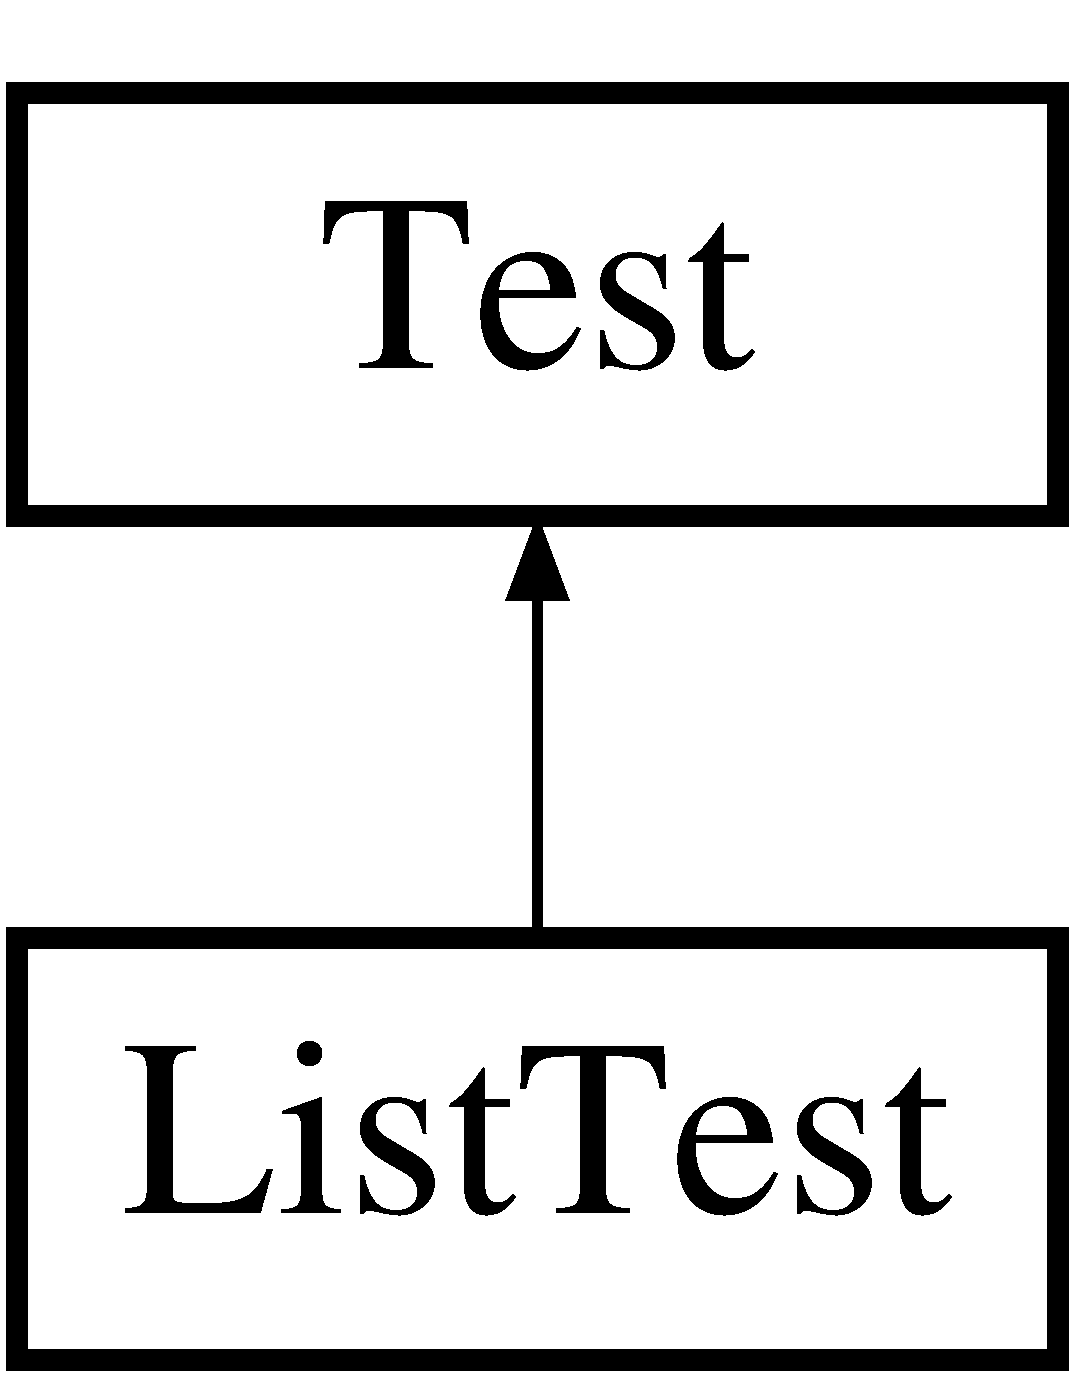
\includegraphics[height=2.000000cm]{classListTest}
\end{center}
\end{figure}
\subsection*{Protected Member Functions}
\begin{DoxyCompactItemize}
\item 
\hypertarget{classListTest_affc2f4cf21beae819fb58f55bb8a27a6}{void {\bfseries Insert\-Obj} ()}\label{classListTest_affc2f4cf21beae819fb58f55bb8a27a6}

\item 
\hypertarget{classListTest_a3f003521f77f0d69ce15c250c9b3110c}{void {\bfseries Delete\-Obj} ()}\label{classListTest_a3f003521f77f0d69ce15c250c9b3110c}

\item 
\hypertarget{classListTest_a6ce63aead1163d5e2921ade6a1416912}{virtual void {\bfseries Set\-Up} ()}\label{classListTest_a6ce63aead1163d5e2921ade6a1416912}

\end{DoxyCompactItemize}
\subsection*{Protected Attributes}
\begin{DoxyCompactItemize}
\item 
\hypertarget{classListTest_ae7f2c29aec56333f92c277820f1e1bee}{\hyperlink{structco__obj__t}{co\-\_\-obj\-\_\-t} $\ast$ {\bfseries List16}}\label{classListTest_ae7f2c29aec56333f92c277820f1e1bee}

\item 
\hypertarget{classListTest_a3710a8726b3583f7dc600cb1377331a8}{\hyperlink{structco__obj__t}{co\-\_\-obj\-\_\-t} $\ast$ {\bfseries List32}}\label{classListTest_a3710a8726b3583f7dc600cb1377331a8}

\end{DoxyCompactItemize}


The documentation for this class was generated from the following file\-:\begin{DoxyCompactItemize}
\item 
tests/list.\-cpp\end{DoxyCompactItemize}

\hypertarget{unionmax__align}{\section{max\+\_\+align Union Reference}
\label{unionmax__align}\index{max\+\_\+align@{max\+\_\+align}}
}
\subsection*{Public Attributes}
\begin{DoxyCompactItemize}
\item 
\hypertarget{unionmax__align_ae0f6c483820acb32266a5a03449874a1}{char {\bfseries c}}\label{unionmax__align_ae0f6c483820acb32266a5a03449874a1}

\item 
\hypertarget{unionmax__align_a786335ebeeca204d9abb1570f1fd9258}{short {\bfseries s}}\label{unionmax__align_a786335ebeeca204d9abb1570f1fd9258}

\item 
\hypertarget{unionmax__align_aec3ccee73d705da2b2fb4987a0cfb88c}{long {\bfseries l}}\label{unionmax__align_aec3ccee73d705da2b2fb4987a0cfb88c}

\item 
\hypertarget{unionmax__align_ae435683bc3acb9d7a5cb8a154e274ed0}{int {\bfseries i}}\label{unionmax__align_ae435683bc3acb9d7a5cb8a154e274ed0}

\item 
\hypertarget{unionmax__align_aef79c8eefe43f54bb746cb66094f9e69}{float {\bfseries f}}\label{unionmax__align_aef79c8eefe43f54bb746cb66094f9e69}

\item 
\hypertarget{unionmax__align_a348f5ea41f081f6fd243ffa6dd1bd820}{double {\bfseries d}}\label{unionmax__align_a348f5ea41f081f6fd243ffa6dd1bd820}

\item 
\hypertarget{unionmax__align_af33cdc78318cd53fd47d8f5331446d30}{void $\ast$ {\bfseries v}}\label{unionmax__align_af33cdc78318cd53fd47d8f5331446d30}

\item 
\hypertarget{unionmax__align_a7ed5d9e65c78c7b5acb2e064cf98e03a}{void($\ast$ {\bfseries q} )(void)}\label{unionmax__align_a7ed5d9e65c78c7b5acb2e064cf98e03a}

\end{DoxyCompactItemize}


The documentation for this union was generated from the following file\+:\begin{DoxyCompactItemize}
\item 
src/extern/align.\+h\end{DoxyCompactItemize}

\hypertarget{structMD5__CTX}{\section{M\-D5\-\_\-\-C\-T\-X Struct Reference}
\label{structMD5__CTX}\index{M\-D5\-\_\-\-C\-T\-X@{M\-D5\-\_\-\-C\-T\-X}}
}
\subsection*{Public Attributes}
\begin{DoxyCompactItemize}
\item 
\hypertarget{structMD5__CTX_a90437ec62a8dda787f1667061d9755fe}{M\-D5\-\_\-u32plus {\bfseries lo}}\label{structMD5__CTX_a90437ec62a8dda787f1667061d9755fe}

\item 
\hypertarget{structMD5__CTX_a3234f683810977ac629c2a8a05a1cc87}{M\-D5\-\_\-u32plus {\bfseries hi}}\label{structMD5__CTX_a3234f683810977ac629c2a8a05a1cc87}

\item 
\hypertarget{structMD5__CTX_abfbd731eb0b9d13a75ee4e49715e30b5}{M\-D5\-\_\-u32plus {\bfseries a}}\label{structMD5__CTX_abfbd731eb0b9d13a75ee4e49715e30b5}

\item 
\hypertarget{structMD5__CTX_a63ef5819a909e0b4065796dfdac25962}{M\-D5\-\_\-u32plus {\bfseries b}}\label{structMD5__CTX_a63ef5819a909e0b4065796dfdac25962}

\item 
\hypertarget{structMD5__CTX_a6226440d9b52200d32153df206fe3761}{M\-D5\-\_\-u32plus {\bfseries c}}\label{structMD5__CTX_a6226440d9b52200d32153df206fe3761}

\item 
\hypertarget{structMD5__CTX_a3b2316dbfcad4bdb1306dc441761f396}{M\-D5\-\_\-u32plus {\bfseries d}}\label{structMD5__CTX_a3b2316dbfcad4bdb1306dc441761f396}

\item 
\hypertarget{structMD5__CTX_a2da73ecf544745f58211e998719f367f}{unsigned char {\bfseries buffer} \mbox{[}64\mbox{]}}\label{structMD5__CTX_a2da73ecf544745f58211e998719f367f}

\item 
\hypertarget{structMD5__CTX_a2db62677a153981a205d225b051f0609}{M\-D5\-\_\-u32plus {\bfseries block} \mbox{[}16\mbox{]}}\label{structMD5__CTX_a2db62677a153981a205d225b051f0609}

\end{DoxyCompactItemize}


The documentation for this struct was generated from the following file\-:\begin{DoxyCompactItemize}
\item 
src/extern/md5.\-h\end{DoxyCompactItemize}

\hypertarget{unionnodeid__t}{\section{nodeid\+\_\+t Struct Reference}
\label{unionnodeid__t}\index{nodeid\+\_\+t@{nodeid\+\_\+t}}
}
\subsection*{Public Attributes}
\begin{DoxyCompactItemize}
\item 
\hypertarget{unionnodeid__t_a1e946677ad39dfeb9944ffce81432ba5}{uint32\+\_\+t {\bfseries id}}\label{unionnodeid__t_a1e946677ad39dfeb9944ffce81432ba5}

\item 
\hypertarget{unionnodeid__t_aaffc442232e5775496b5e322a9653a3b}{uint8\+\_\+t {\bfseries bytes} \mbox{[}4\mbox{]}}\label{unionnodeid__t_aaffc442232e5775496b5e322a9653a3b}

\end{DoxyCompactItemize}


\subsection{Detailed Description}
node id and last four bytes of M\+A\+C address 

The documentation for this struct was generated from the following file\+:\begin{DoxyCompactItemize}
\item 
src/\hyperlink{id_8h}{id.\+h}\end{DoxyCompactItemize}

\hypertarget{structsvl__crypto__ctx}{\section{svl\+\_\+crypto\+\_\+ctx Struct Reference}
\label{structsvl__crypto__ctx}\index{svl\+\_\+crypto\+\_\+ctx@{svl\+\_\+crypto\+\_\+ctx}}
}
\subsection*{Public Attributes}
\begin{DoxyCompactItemize}
\item 
\hypertarget{structsvl__crypto__ctx_ad8980dd54ef8e577c38f1840a1a1460c}{char $\ast$ {\bfseries keyring\+\_\+path}}\label{structsvl__crypto__ctx_ad8980dd54ef8e577c38f1840a1a1460c}

\item 
\hypertarget{structsvl__crypto__ctx_a5a6d4a9d6a466047528b6c4fb9d408e1}{size\+\_\+t {\bfseries keyring\+\_\+len}}\label{structsvl__crypto__ctx_a5a6d4a9d6a466047528b6c4fb9d408e1}

\item 
\hypertarget{structsvl__crypto__ctx_a7ab514ea2330d07c03e9dd18924b5d3b}{keyring\+\_\+file $\ast$ {\bfseries keyring\+\_\+file}}\label{structsvl__crypto__ctx_a7ab514ea2330d07c03e9dd18924b5d3b}

\item 
\hypertarget{structsvl__crypto__ctx_a56a6ffa4afdbce4b218637cb1e554660}{unsigned char {\bfseries sid} \mbox{[}S\+I\+D\+\_\+\+S\+I\+Z\+E\mbox{]}}\label{structsvl__crypto__ctx_a56a6ffa4afdbce4b218637cb1e554660}

\item 
\hypertarget{structsvl__crypto__ctx_aa073486cf89574d65ef3c0660b3ec9c0}{unsigned char {\bfseries sas\+\_\+public} \mbox{[}crypto\+\_\+sign\+\_\+\+P\+U\+B\+L\+I\+C\+K\+E\+Y\+B\+Y\+T\+E\+S\mbox{]}}\label{structsvl__crypto__ctx_aa073486cf89574d65ef3c0660b3ec9c0}

\item 
\hypertarget{structsvl__crypto__ctx_a3f476ccc11a0c28552877358e6f64d30}{unsigned char {\bfseries sas\+\_\+private} \mbox{[}crypto\+\_\+sign\+\_\+\+S\+E\+C\+R\+E\+T\+K\+E\+Y\+B\+Y\+T\+E\+S\mbox{]}}\label{structsvl__crypto__ctx_a3f476ccc11a0c28552877358e6f64d30}

\item 
\hypertarget{structsvl__crypto__ctx_aa5a5a1490bff146660c77951fc0e2e98}{unsigned char {\bfseries signature} \mbox{[}S\+I\+G\+N\+A\+T\+U\+R\+E\+\_\+\+B\+Y\+T\+E\+S\mbox{]}}\label{structsvl__crypto__ctx_aa5a5a1490bff146660c77951fc0e2e98}

\item 
\hypertarget{structsvl__crypto__ctx_aa3e2e9b87b39af964921175ede10c7e4}{unsigned char $\ast$ {\bfseries msg}}\label{structsvl__crypto__ctx_aa3e2e9b87b39af964921175ede10c7e4}

\item 
\hypertarget{structsvl__crypto__ctx_ab2897ce3e55a5dbd3c13db58cfa4e374}{size\+\_\+t {\bfseries msg\+\_\+len}}\label{structsvl__crypto__ctx_ab2897ce3e55a5dbd3c13db58cfa4e374}

\end{DoxyCompactItemize}


The documentation for this struct was generated from the following file\+:\begin{DoxyCompactItemize}
\item 
plugins/serval-\/dna/\hyperlink{crypto_8h}{crypto.\+h}\end{DoxyCompactItemize}

\hypertarget{classTreeTest}{\section{Tree\-Test Class Reference}
\label{classTreeTest}\index{Tree\-Test@{Tree\-Test}}
}
Inheritance diagram for Tree\-Test\-:\begin{figure}[H]
\begin{center}
\leavevmode
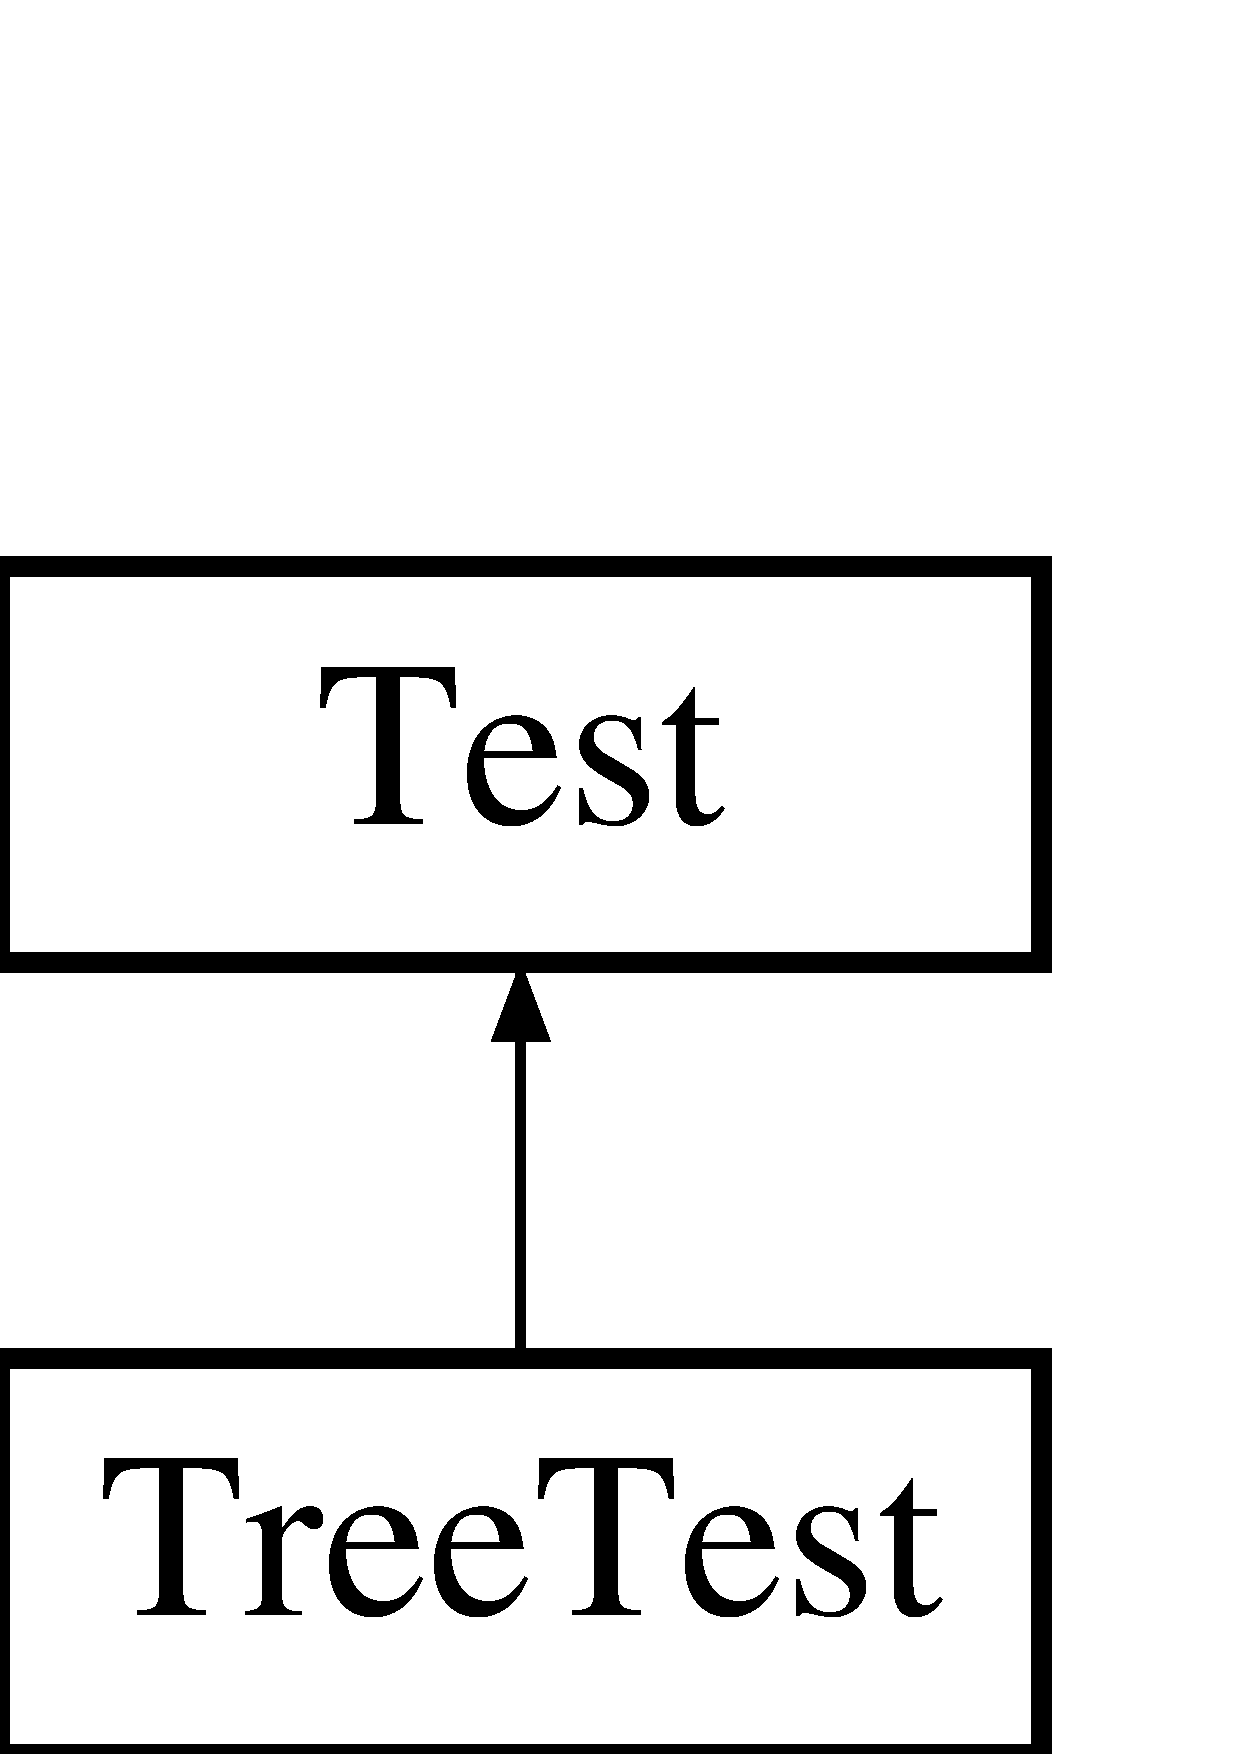
\includegraphics[height=2.000000cm]{classTreeTest}
\end{center}
\end{figure}
\subsection*{Protected Member Functions}
\begin{DoxyCompactItemize}
\item 
\hypertarget{classTreeTest_adaa57828d45a89aadacd259a0e69790a}{void {\bfseries Insert\-Obj} ()}\label{classTreeTest_adaa57828d45a89aadacd259a0e69790a}

\item 
\hypertarget{classTreeTest_a9ab561b627cc999d4c89f94ea53d291b}{void {\bfseries Delete\-Obj} ()}\label{classTreeTest_a9ab561b627cc999d4c89f94ea53d291b}

\item 
\hypertarget{classTreeTest_ae5d5b1281cfa1438ba792ae65f0f6341}{void {\bfseries Update\-Obj} ()}\label{classTreeTest_ae5d5b1281cfa1438ba792ae65f0f6341}

\item 
\hypertarget{classTreeTest_a50caa23d3a9be5549c5b26fe78412602}{virtual void {\bfseries Set\-Up} ()}\label{classTreeTest_a50caa23d3a9be5549c5b26fe78412602}

\end{DoxyCompactItemize}
\subsection*{Protected Attributes}
\begin{DoxyCompactItemize}
\item 
\hypertarget{classTreeTest_a262dbb122877911eb0a8a2c79abc891e}{\hyperlink{structco__obj__t}{co\-\_\-obj\-\_\-t} $\ast$ {\bfseries Tree16}}\label{classTreeTest_a262dbb122877911eb0a8a2c79abc891e}

\item 
\hypertarget{classTreeTest_a03999420e4ce83dd4440f255e592d8c0}{\hyperlink{structco__obj__t}{co\-\_\-obj\-\_\-t} $\ast$ {\bfseries Tree32}}\label{classTreeTest_a03999420e4ce83dd4440f255e592d8c0}

\item 
\hypertarget{classTreeTest_aa65307950ea381fcccf0c89c02d6e5e3}{\hyperlink{structco__obj__t}{co\-\_\-obj\-\_\-t} $\ast$ {\bfseries Test\-String1}}\label{classTreeTest_aa65307950ea381fcccf0c89c02d6e5e3}

\item 
\hypertarget{classTreeTest_a0eb58bddd27d6f74d1ec72bba967e3fc}{\hyperlink{structco__obj__t}{co\-\_\-obj\-\_\-t} $\ast$ {\bfseries Test\-String2}}\label{classTreeTest_a0eb58bddd27d6f74d1ec72bba967e3fc}

\item 
\hypertarget{classTreeTest_a2cadc4638b7aa4bebe3b233b5dad4bfc}{\hyperlink{structco__obj__t}{co\-\_\-obj\-\_\-t} $\ast$ {\bfseries Replace\-String1}}\label{classTreeTest_a2cadc4638b7aa4bebe3b233b5dad4bfc}

\item 
\hypertarget{classTreeTest_a30311c961c18b22dc91ecb9da8939c93}{\hyperlink{structco__obj__t}{co\-\_\-obj\-\_\-t} $\ast$ {\bfseries Test\-String3}}\label{classTreeTest_a30311c961c18b22dc91ecb9da8939c93}

\item 
\hypertarget{classTreeTest_a3ea8dde968a96f26b4d79082498e7812}{\hyperlink{structco__obj__t}{co\-\_\-obj\-\_\-t} $\ast$ {\bfseries ptr}}\label{classTreeTest_a3ea8dde968a96f26b4d79082498e7812}

\item 
\hypertarget{classTreeTest_ae7d983b14a020f8f7a4d661626f67863}{int {\bfseries ret}}\label{classTreeTest_ae7d983b14a020f8f7a4d661626f67863}

\end{DoxyCompactItemize}


The documentation for this class was generated from the following file\-:\begin{DoxyCompactItemize}
\item 
tests/tree.\-cpp\end{DoxyCompactItemize}

\hypertarget{structunix__socket__t}{\section{unix\+\_\+socket\+\_\+t Struct Reference}
\label{structunix__socket__t}\index{unix\+\_\+socket\+\_\+t@{unix\+\_\+socket\+\_\+t}}
}
\subsection*{Public Attributes}
\begin{DoxyCompactItemize}
\item 
\hypertarget{structunix__socket__t_a2d7a292e061c3731747973ae1f97f292}{\hyperlink{structco__socket__t}{co\+\_\+socket\+\_\+t} {\bfseries proto}}\label{structunix__socket__t_a2d7a292e061c3731747973ae1f97f292}

\item 
\hypertarget{structunix__socket__t_a237d9703b3ad03932aea8635e635b043}{char $\ast$ {\bfseries path}}\label{structunix__socket__t_a237d9703b3ad03932aea8635e635b043}

\end{DoxyCompactItemize}


\subsection{Detailed Description}
unix sockets. Contains protocol and file path to socket library 

The documentation for this struct was generated from the following file\+:\begin{DoxyCompactItemize}
\item 
src/\hyperlink{socket_8h}{socket.\+h}\end{DoxyCompactItemize}

\hypertarget{structwpa__ctrl}{\section{wpa\-\_\-ctrl Struct Reference}
\label{structwpa__ctrl}\index{wpa\-\_\-ctrl@{wpa\-\_\-ctrl}}
}
\subsection*{Public Attributes}
\begin{DoxyCompactItemize}
\item 
\hypertarget{structwpa__ctrl_ac5d2fbfbd7247dcdbd6b271419465ee8}{int {\bfseries s}}\label{structwpa__ctrl_ac5d2fbfbd7247dcdbd6b271419465ee8}

\item 
\hypertarget{structwpa__ctrl_ab91fe974613c7fab068f3751cfcb094f}{struct sockaddr\-\_\-un {\bfseries local}}\label{structwpa__ctrl_ab91fe974613c7fab068f3751cfcb094f}

\item 
\hypertarget{structwpa__ctrl_a8817e5e94060f2ee19889f7fdafa8273}{struct sockaddr\-\_\-un {\bfseries dest}}\label{structwpa__ctrl_a8817e5e94060f2ee19889f7fdafa8273}

\end{DoxyCompactItemize}


\subsection{Detailed Description}
strlcpy -\/ Copy a string with size bound and N\-U\-L-\/termination \-: Destination \-: Source \-: Size of the target buffer Returns\-: Total length of the target string (length of src) (not including N\-U\-L-\/termination)

This function matches in behavior with the strlcpy(3) function in Open\-B\-S\-D. struct \hyperlink{structwpa__ctrl}{wpa\-\_\-ctrl} -\/ Internal structure for control interface library

This structure is used by the wpa\-\_\-supplicant/hostapd control interface library to store internal data. Programs using the library should not touch this data directly. They can only use the pointer to the data structure as an identifier for the control interface connection and use this as one of the arguments for most of the control interface library functions. 

The documentation for this struct was generated from the following file\-:\begin{DoxyCompactItemize}
\item 
src/extern/wpa\-\_\-ctrl.\-c\end{DoxyCompactItemize}

\chapter{File Documentation}
\hypertarget{olsrd_8c}{\section{plugins/olsrd/olsrd.c File Reference}
\label{olsrd_8c}\index{plugins/olsrd/olsrd.\-c@{plugins/olsrd/olsrd.\-c}}
}


O\-L\-S\-Rd configuration and process management.  


{\ttfamily \#include $<$stdlib.\-h$>$}\\*
{\ttfamily \#include \char`\"{}extern/list.\-h\char`\"{}}\\*
{\ttfamily \#include \char`\"{}debug.\-h\char`\"{}}\\*
{\ttfamily \#include \char`\"{}util.\-h\char`\"{}}\\*
{\ttfamily \#include \char`\"{}olsrd.\-h\char`\"{}}\\*
\subsection*{Functions}
\begin{DoxyCompactItemize}
\item 
int \hyperlink{olsrd_8c_a81d06fa13f5f770648b1d397a45425a3}{co\-\_\-olsrd\-\_\-print\-\_\-conf} (const char $\ast$filename)
\begin{DoxyCompactList}\small\item\em prints O\-L\-S\-R configuration info from file (currently unimplemented) \end{DoxyCompactList}\item 
int \hyperlink{olsrd_8c_a39e013d74b514b6eed083b0241214cc0}{co\-\_\-olsrd\-\_\-add\-\_\-iface} (const char $\ast$\hyperlink{profile_8h_a842efb72cde7678fc8a8162084b327ea}{name}, int mode, const char $\ast$Ipv4\-Broadcast)
\begin{DoxyCompactList}\small\item\em adds an interface to O\-L\-S\-Rd \end{DoxyCompactList}\item 
int \hyperlink{olsrd_8c_a61065305edbe37e889d398373b27c1f5}{co\-\_\-olsrd\-\_\-remove\-\_\-iface} (char $\ast$\hyperlink{profile_8h_a842efb72cde7678fc8a8162084b327ea}{name}, int mode, char $\ast$Ipv4\-Broadcast)
\begin{DoxyCompactList}\small\item\em removes an interface from O\-L\-S\-Rd \end{DoxyCompactList}\item 
int \hyperlink{olsrd_8c_a82dd6adc08598d10d042028ad12f1b3a}{co\-\_\-olsrd\-\_\-add\-\_\-hna} (const int family, const char $\ast$address, const char $\ast$netmask)
\begin{DoxyCompactList}\small\item\em adds a host network address to O\-L\-S\-Rd \end{DoxyCompactList}\item 
int \hyperlink{olsrd_8c_accc2c9b50b83de414d11262d2ccf6fab}{co\-\_\-olsrd\-\_\-remove\-\_\-hna} (int family, char $\ast$address, char $\ast$netmask)
\begin{DoxyCompactList}\small\item\em remves a host network address from O\-L\-S\-Rd \end{DoxyCompactList}\item 
int \hyperlink{olsrd_8c_a59de4356b3a842ee61130136360ebd95}{co\-\_\-olsrd\-\_\-init} (\hyperlink{structco__obj__t}{co\-\_\-obj\-\_\-t} $\ast$self)
\begin{DoxyCompactList}\small\item\em initiates the O\-L\-S\-R daemon when a new process gets created (currently unimplemented) \end{DoxyCompactList}\end{DoxyCompactItemize}
\subsection*{Variables}
\begin{DoxyCompactItemize}
\item 
\hyperlink{structco__process__t}{co\-\_\-process\-\_\-t} {\bfseries olsrd\-\_\-process\-\_\-proto}
\end{DoxyCompactItemize}


\subsection{Detailed Description}
O\-L\-S\-Rd configuration and process management. \begin{DoxyAuthor}{Author}
Josh King (jheretic), \href{mailto:jking@chambana.net}{\tt jking@chambana.\-net} 
\end{DoxyAuthor}


\subsection{Function Documentation}
\hypertarget{olsrd_8c_a82dd6adc08598d10d042028ad12f1b3a}{\index{olsrd.\-c@{olsrd.\-c}!co\-\_\-olsrd\-\_\-add\-\_\-hna@{co\-\_\-olsrd\-\_\-add\-\_\-hna}}
\index{co\-\_\-olsrd\-\_\-add\-\_\-hna@{co\-\_\-olsrd\-\_\-add\-\_\-hna}!olsrd.c@{olsrd.\-c}}
\subsubsection[{co\-\_\-olsrd\-\_\-add\-\_\-hna}]{\setlength{\rightskip}{0pt plus 5cm}int co\-\_\-olsrd\-\_\-add\-\_\-hna (
\begin{DoxyParamCaption}
\item[{const int}]{family, }
\item[{const char $\ast$}]{address, }
\item[{const char $\ast$}]{netmask}
\end{DoxyParamCaption}
)}}\label{olsrd_8c_a82dd6adc08598d10d042028ad12f1b3a}


adds a host network address to O\-L\-S\-Rd 


\begin{DoxyParams}{Parameters}
{\em family} & the address family \\
\hline
{\em address} & the network address for the interface \\
\hline
{\em netmask} & the netmask for the interface \\
\hline
\end{DoxyParams}

\begin{DoxyCode}
198                                                                                  \{
199   \hyperlink{structco__olsrd__conf__hna__t}{co\_olsrd\_conf\_hna\_t} *new\_hna = NULL;
200   new\_hna = (\hyperlink{structco__olsrd__conf__hna__t}{co\_olsrd\_conf\_hna\_t}*)calloc(1, \textcolor{keyword}{sizeof}(
      \hyperlink{structco__olsrd__conf__hna__t}{co\_olsrd\_conf\_hna\_t}));
201 
202   new\_hna->family = family;
203 
204   new\_hna->address = (\textcolor{keywordtype}{char}*)calloc(strlen(address)+1, \textcolor{keyword}{sizeof}(char));
205   strcpy(new\_hna->address, address);
206   
207   new\_hna->netmask = (\textcolor{keywordtype}{char}*)calloc(strlen(netmask)+1, \textcolor{keyword}{sizeof}(char));
208   strcpy(new\_hna->netmask, netmask);
209 
210   list\_append(hna, lnode\_create(new\_hna));
211   \textcolor{keywordflow}{return} 1;
212 \}
\end{DoxyCode}
\hypertarget{olsrd_8c_a39e013d74b514b6eed083b0241214cc0}{\index{olsrd.\-c@{olsrd.\-c}!co\-\_\-olsrd\-\_\-add\-\_\-iface@{co\-\_\-olsrd\-\_\-add\-\_\-iface}}
\index{co\-\_\-olsrd\-\_\-add\-\_\-iface@{co\-\_\-olsrd\-\_\-add\-\_\-iface}!olsrd.c@{olsrd.\-c}}
\subsubsection[{co\-\_\-olsrd\-\_\-add\-\_\-iface}]{\setlength{\rightskip}{0pt plus 5cm}int co\-\_\-olsrd\-\_\-add\-\_\-iface (
\begin{DoxyParamCaption}
\item[{const char $\ast$}]{name, }
\item[{int}]{mode, }
\item[{const char $\ast$}]{Ipv4\-Broadcast}
\end{DoxyParamCaption}
)}}\label{olsrd_8c_a39e013d74b514b6eed083b0241214cc0}


adds an interface to O\-L\-S\-Rd 


\begin{DoxyParams}{Parameters}
{\em name} & name of the interface to be added \\
\hline
{\em mode} & network mode for interface \\
\hline
{\em Ipv4\-Broadcast} & I\-Pv4 broadcast address (node address, using netmask as last octet) \\
\hline
\end{DoxyParams}

\begin{DoxyCode}
149                                                                               \{
150   \hyperlink{structco__olsrd__conf__iface__t}{co\_olsrd\_conf\_iface\_t} *new\_iface = NULL;
151   new\_iface = (\hyperlink{structco__olsrd__conf__iface__t}{co\_olsrd\_conf\_iface\_t}*)calloc(1, \textcolor{keyword}{sizeof}(
      \hyperlink{structco__olsrd__conf__iface__t}{co\_olsrd\_conf\_iface\_t}));
152 
153   new\_iface->mode = mode;
154 
155   new\_iface->ifname = (\textcolor{keywordtype}{char}*)calloc(strlen(\hyperlink{cmd_8h_a842efb72cde7678fc8a8162084b327ea}{name})+1, \textcolor{keyword}{sizeof}(char));
156   strcpy(new\_iface->ifname, \hyperlink{cmd_8h_a842efb72cde7678fc8a8162084b327ea}{name});
157 
158   new\_iface->Ipv4Broadcast=(\textcolor{keywordtype}{char}*)calloc(strlen(Ipv4Broadcast)+1,\textcolor{keyword}{sizeof}(char));
159   strcpy(new\_iface->Ipv4Broadcast, Ipv4Broadcast);
160 
161   list\_append(ifaces, lnode\_create(new\_iface));
162   \textcolor{keywordflow}{return} 1;
163 \}
\end{DoxyCode}
\hypertarget{olsrd_8c_a59de4356b3a842ee61130136360ebd95}{\index{olsrd.\-c@{olsrd.\-c}!co\-\_\-olsrd\-\_\-init@{co\-\_\-olsrd\-\_\-init}}
\index{co\-\_\-olsrd\-\_\-init@{co\-\_\-olsrd\-\_\-init}!olsrd.c@{olsrd.\-c}}
\subsubsection[{co\-\_\-olsrd\-\_\-init}]{\setlength{\rightskip}{0pt plus 5cm}int co\-\_\-olsrd\-\_\-init (
\begin{DoxyParamCaption}
\item[{{\bf co\-\_\-obj\-\_\-t} $\ast$}]{self}
\end{DoxyParamCaption}
)}}\label{olsrd_8c_a59de4356b3a842ee61130136360ebd95}


initiates the O\-L\-S\-R daemon when a new process gets created (currently unimplemented) 


\begin{DoxyParams}{Parameters}
{\em self} & process to be called \\
\hline
\end{DoxyParams}

\begin{DoxyCode}
248                                   \{
249   \textcolor{comment}{//co\_olsrd\_process\_t *this = self;}
250   \textcolor{comment}{//This function gets called when the process object is created, and should call any initialization stuff
       that happens before it starts}
251   \textcolor{keywordflow}{return} 1;
252 \}
\end{DoxyCode}
\hypertarget{olsrd_8c_a81d06fa13f5f770648b1d397a45425a3}{\index{olsrd.\-c@{olsrd.\-c}!co\-\_\-olsrd\-\_\-print\-\_\-conf@{co\-\_\-olsrd\-\_\-print\-\_\-conf}}
\index{co\-\_\-olsrd\-\_\-print\-\_\-conf@{co\-\_\-olsrd\-\_\-print\-\_\-conf}!olsrd.c@{olsrd.\-c}}
\subsubsection[{co\-\_\-olsrd\-\_\-print\-\_\-conf}]{\setlength{\rightskip}{0pt plus 5cm}int co\-\_\-olsrd\-\_\-print\-\_\-conf (
\begin{DoxyParamCaption}
\item[{const char $\ast$}]{filename}
\end{DoxyParamCaption}
)}}\label{olsrd_8c_a81d06fa13f5f770648b1d397a45425a3}


prints O\-L\-S\-R configuration info from file (currently unimplemented) 


\begin{DoxyParams}{Parameters}
{\em filename} & the configuration file \\
\hline
\end{DoxyParams}


References name.


\begin{DoxyCode}
93                                               \{
94   \textcolor{keywordtype}{int} i = 0;
95   FILE *conf\_file;
96 
97   \textcolor{keywordflow}{if} (!(conf\_file = fopen(filename, \textcolor{stringliteral}{"w+"}))) \{
98     \textcolor{comment}{/* file could not be opened!}
99 \textcolor{comment}{     */}
100     \textcolor{keywordflow}{return} 0;
101   \}
102 
103   \textcolor{keywordflow}{for} (i = 0; i<global\_items\_count; i++) \{
104     fprintf(conf\_file, \textcolor{stringliteral}{"%s\(\backslash\)t%s\(\backslash\)n"}, global\_items[i].key, 
105                                    global\_items[i].value);
106   \}
107 
108   \textcolor{keywordflow}{for} (i = 0; i<plugins\_count; i++) \{
109     \textcolor{keywordtype}{int} j = 0;
110     fprintf(conf\_file, \textcolor{stringliteral}{"LoadPlugin\(\backslash\)t\(\backslash\)"%s\(\backslash\)"\(\backslash\)n"}, plugins[i].\hyperlink{cmd_8h_a842efb72cde7678fc8a8162084b327ea}{name});
111     fprintf(conf\_file, \textcolor{stringliteral}{"\{\(\backslash\)n"});
112     \textcolor{keywordflow}{for} (j = 0; j<plugins[i].num\_attr; j++) \{
113       fprintf(conf\_file, \textcolor{stringliteral}{"\(\backslash\)t%s\(\backslash\)t%s\(\backslash\)n"},plugins[i].attr[i]->key, 
114                                       plugins[i].attr[i]->value);
115     \}
116     fprintf(conf\_file, \textcolor{stringliteral}{"\}\(\backslash\)n"});
117   \}
118 
119   list\_process(ifaces, (\textcolor{keywordtype}{void}*)conf\_file, \_co\_olsrd\_print\_iface\_i);
120   list\_process(hna, (\textcolor{keywordtype}{void}*)conf\_file, \_co\_olsrd\_print\_hna\_i);
121 
122   fclose(conf\_file);
123 
124   \textcolor{keywordflow}{return} 1;
125 \}
\end{DoxyCode}
\hypertarget{olsrd_8c_accc2c9b50b83de414d11262d2ccf6fab}{\index{olsrd.\-c@{olsrd.\-c}!co\-\_\-olsrd\-\_\-remove\-\_\-hna@{co\-\_\-olsrd\-\_\-remove\-\_\-hna}}
\index{co\-\_\-olsrd\-\_\-remove\-\_\-hna@{co\-\_\-olsrd\-\_\-remove\-\_\-hna}!olsrd.c@{olsrd.\-c}}
\subsubsection[{co\-\_\-olsrd\-\_\-remove\-\_\-hna}]{\setlength{\rightskip}{0pt plus 5cm}int co\-\_\-olsrd\-\_\-remove\-\_\-hna (
\begin{DoxyParamCaption}
\item[{int}]{family, }
\item[{char $\ast$}]{address, }
\item[{char $\ast$}]{netmask}
\end{DoxyParamCaption}
)}}\label{olsrd_8c_accc2c9b50b83de414d11262d2ccf6fab}


remves a host network address from O\-L\-S\-Rd 


\begin{DoxyParams}{Parameters}
{\em family} & the address family \\
\hline
{\em address} & the network address for the interface \\
\hline
{\em netmask} & the netmask for the interface \\
\hline
\end{DoxyParams}

\begin{DoxyCode}
214                                                                   \{
215   \hyperlink{structco__olsrd__conf__hna__t}{co\_olsrd\_conf\_hna\_t} *hna\_to\_remove;
216   \hyperlink{structco__olsrd__conf__hna__t}{co\_olsrd\_conf\_hna\_t} hna\_to\_find;
217   lnode\_t *hna\_node\_to\_remove;
218 
219   \textcolor{comment}{/*}
220 \textcolor{comment}{   * FYI: This causes a compiler warning for}
221 \textcolor{comment}{   * discarding the constant. Using a strcpy()}
222 \textcolor{comment}{   * would fix this, but that wastes time.}
223 \textcolor{comment}{   */}
224   hna\_to\_find.family = family;
225   hna\_to\_find.address = address;
226   hna\_to\_find.netmask = netmask;
227 
228   \textcolor{keywordflow}{if} ((hna\_node\_to\_remove = list\_find(hna, 
229                                      &hna\_to\_find, 
230                                      \_co\_olsrd\_compare\_hna\_i))) \{
231     \textcolor{comment}{/* }
232 \textcolor{comment}{     * delete from the list.}
233 \textcolor{comment}{     */}
234     list\_delete(hna, hna\_node\_to\_remove);
235 
236     \textcolor{comment}{/*}
237 \textcolor{comment}{     * free the object's memory.}
238 \textcolor{comment}{     */}
239     hna\_to\_remove = lnode\_get(hna\_node\_to\_remove);
240     free(hna\_to\_remove->address);
241     free(hna\_to\_remove->netmask);
242     free(hna\_to\_remove);
243   \}
244   \textcolor{keywordflow}{return} 1;
245 \}
\end{DoxyCode}
\hypertarget{olsrd_8c_a61065305edbe37e889d398373b27c1f5}{\index{olsrd.\-c@{olsrd.\-c}!co\-\_\-olsrd\-\_\-remove\-\_\-iface@{co\-\_\-olsrd\-\_\-remove\-\_\-iface}}
\index{co\-\_\-olsrd\-\_\-remove\-\_\-iface@{co\-\_\-olsrd\-\_\-remove\-\_\-iface}!olsrd.c@{olsrd.\-c}}
\subsubsection[{co\-\_\-olsrd\-\_\-remove\-\_\-iface}]{\setlength{\rightskip}{0pt plus 5cm}int co\-\_\-olsrd\-\_\-remove\-\_\-iface (
\begin{DoxyParamCaption}
\item[{char $\ast$}]{name, }
\item[{int}]{mode, }
\item[{char $\ast$}]{Ipv4\-Broadcast}
\end{DoxyParamCaption}
)}}\label{olsrd_8c_a61065305edbe37e889d398373b27c1f5}


removes an interface from O\-L\-S\-Rd 


\begin{DoxyParams}{Parameters}
{\em name} & name of the interface to be removed \\
\hline
{\em mode} & network mode for interface \\
\hline
{\em Ipv4\-Broadcast} & I\-Pv4 broadcast address (node address, using netmask as last octet) \\
\hline
\end{DoxyParams}


References name.


\begin{DoxyCode}
165                                                                      \{
166   \hyperlink{structco__olsrd__conf__iface__t}{co\_olsrd\_conf\_iface\_t} *iface\_to\_remove;
167   \hyperlink{structco__olsrd__conf__iface__t}{co\_olsrd\_conf\_iface\_t} iface\_to\_find;
168   lnode\_t *iface\_node\_to\_remove;
169 
170   \textcolor{comment}{/*}
171 \textcolor{comment}{   * FYI: This causes a compiler warning for}
172 \textcolor{comment}{   * discarding the constant. Using a strcpy()}
173 \textcolor{comment}{   * would fix this, but that wastes time.}
174 \textcolor{comment}{   */}
175   iface\_to\_find.mode = mode;
176   iface\_to\_find.ifname = \hyperlink{cmd_8h_a842efb72cde7678fc8a8162084b327ea}{name};
177   iface\_to\_find.Ipv4Broadcast = Ipv4Broadcast;
178 
179   \textcolor{keywordflow}{if} ((iface\_node\_to\_remove = list\_find(ifaces, 
180                                        &iface\_to\_find, 
181                                        \_co\_olsrd\_compare\_iface\_i))) \{
182     \textcolor{comment}{/* }
183 \textcolor{comment}{     * delete from the list.}
184 \textcolor{comment}{     */}
185     list\_delete(ifaces, iface\_node\_to\_remove);
186 
187     \textcolor{comment}{/*}
188 \textcolor{comment}{     * free the object's memory.}
189 \textcolor{comment}{     */}
190     iface\_to\_remove = lnode\_get(iface\_node\_to\_remove);
191     free(iface\_to\_remove->ifname);
192     free(iface\_to\_remove->Ipv4Broadcast);
193     free(iface\_to\_remove);
194   \}
195   \textcolor{keywordflow}{return} 1;
196 \}
\end{DoxyCode}


\subsection{Variable Documentation}
\hypertarget{olsrd_8c_a526baf67912f9fea761874a336c3f0d9}{\index{olsrd.\-c@{olsrd.\-c}!olsrd\-\_\-process\-\_\-proto@{olsrd\-\_\-process\-\_\-proto}}
\index{olsrd\-\_\-process\-\_\-proto@{olsrd\-\_\-process\-\_\-proto}!olsrd.c@{olsrd.\-c}}
\subsubsection[{olsrd\-\_\-process\-\_\-proto}]{\setlength{\rightskip}{0pt plus 5cm}{\bf co\-\_\-process\-\_\-t} olsrd\-\_\-process\-\_\-proto}}\label{olsrd_8c_a526baf67912f9fea761874a336c3f0d9}
{\bfseries Initial value\-:}
\begin{DoxyCode}
= \{
  .init = \hyperlink{olsrd_8c_a59de4356b3a842ee61130136360ebd95}{co\_olsrd\_init}
\}
\end{DoxyCode}

\hypertarget{olsrd_8h}{\section{plugins/olsrd/olsrd.h File Reference}
\label{olsrd_8h}\index{plugins/olsrd/olsrd.\-h@{plugins/olsrd/olsrd.\-h}}
}


O\-L\-S\-Rd configuration and process management.  


{\ttfamily \#include $<$stdlib.\-h$>$}\\*
{\ttfamily \#include \char`\"{}process.\-h\char`\"{}}\\*
{\ttfamily \#include \char`\"{}util.\-h\char`\"{}}\\*
{\ttfamily \#include \char`\"{}obj.\-h\char`\"{}}\\*
\subsection*{Classes}
\begin{DoxyCompactItemize}
\item 
struct \hyperlink{structco__olsrd__process__t}{co\-\_\-olsrd\-\_\-process\-\_\-t}
\begin{DoxyCompactList}\small\item\em contains the O\-L\-S\-Rd process protocol \end{DoxyCompactList}\item 
struct \hyperlink{structco__olsrd__conf__item__t}{co\-\_\-olsrd\-\_\-conf\-\_\-item\-\_\-t}
\begin{DoxyCompactList}\small\item\em contains the key and value for configuring O\-L\-S\-Rd for Commotion \end{DoxyCompactList}\item 
struct \hyperlink{structco__olsrd__conf__plugin__t}{co\-\_\-olsrd\-\_\-conf\-\_\-plugin\-\_\-t}
\begin{DoxyCompactList}\small\item\em contains the number of configuration items for O\-L\-S\-Rd \end{DoxyCompactList}\item 
struct \hyperlink{structco__olsrd__conf__iface__t}{co\-\_\-olsrd\-\_\-conf\-\_\-iface\-\_\-t}
\begin{DoxyCompactList}\small\item\em contains interace configuration settings for O\-L\-S\-R, including interface name, mode and I\-Pv4 broadcast message \end{DoxyCompactList}\item 
struct \hyperlink{structco__olsrd__conf__hna__t}{co\-\_\-olsrd\-\_\-conf\-\_\-hna\-\_\-t}
\begin{DoxyCompactList}\small\item\em contains host network address settings, including family, address and netmask \end{DoxyCompactList}\end{DoxyCompactItemize}
\subsection*{Macros}
\begin{DoxyCompactItemize}
\item 
\hypertarget{olsrd_8h_ac25740359eb01e6a2e18ee5b37207081}{\#define {\bfseries O\-L\-S\-R\-\_\-\-H\-N\-A4}~(1 $<$$<$ 0)}\label{olsrd_8h_ac25740359eb01e6a2e18ee5b37207081}

\item 
\hypertarget{olsrd_8h_a923e5ca80f3cd7f82fd29375c66bfa22}{\#define {\bfseries O\-L\-S\-R\-\_\-\-H\-N\-A6}~(1 $<$$<$ 1)}\label{olsrd_8h_a923e5ca80f3cd7f82fd29375c66bfa22}

\item 
\hypertarget{olsrd_8h_a8888f08e61284c00f23b7e7b52d33ad3}{\#define {\bfseries O\-L\-S\-R\-\_\-\-I\-F\-A\-C\-E\-\_\-\-M\-E\-S\-H}~(1 $<$$<$ 0)}\label{olsrd_8h_a8888f08e61284c00f23b7e7b52d33ad3}

\item 
\hypertarget{olsrd_8h_a8dc041750516a6063469e168a2615d35}{\#define {\bfseries O\-L\-S\-R\-\_\-\-I\-F\-A\-C\-E\-\_\-\-E\-T\-H\-E\-R}~(1 $<$$<$ 1)}\label{olsrd_8h_a8dc041750516a6063469e168a2615d35}

\end{DoxyCompactItemize}
\subsection*{Functions}
\begin{DoxyCompactItemize}
\item 
int \hyperlink{olsrd_8h_a39e013d74b514b6eed083b0241214cc0}{co\-\_\-olsrd\-\_\-add\-\_\-iface} (const char $\ast$\hyperlink{profile_8h_a842efb72cde7678fc8a8162084b327ea}{name}, int mode, const char $\ast$Ipv4\-Broadcast)
\begin{DoxyCompactList}\small\item\em adds an interface to O\-L\-S\-Rd \end{DoxyCompactList}\item 
int \hyperlink{olsrd_8h_a61065305edbe37e889d398373b27c1f5}{co\-\_\-olsrd\-\_\-remove\-\_\-iface} (char $\ast$\hyperlink{profile_8h_a842efb72cde7678fc8a8162084b327ea}{name}, int mode, char $\ast$Ipv4\-Broadcast)
\begin{DoxyCompactList}\small\item\em removes an interface from O\-L\-S\-Rd \end{DoxyCompactList}\item 
int \hyperlink{olsrd_8h_a82dd6adc08598d10d042028ad12f1b3a}{co\-\_\-olsrd\-\_\-add\-\_\-hna} (const int family, const char $\ast$address, const char $\ast$netmask)
\begin{DoxyCompactList}\small\item\em adds a host network address to O\-L\-S\-Rd \end{DoxyCompactList}\item 
int \hyperlink{olsrd_8h_accc2c9b50b83de414d11262d2ccf6fab}{co\-\_\-olsrd\-\_\-remove\-\_\-hna} (int family, char $\ast$address, char $\ast$netmask)
\begin{DoxyCompactList}\small\item\em remves a host network address from O\-L\-S\-Rd \end{DoxyCompactList}\item 
int \hyperlink{olsrd_8h_a81d06fa13f5f770648b1d397a45425a3}{co\-\_\-olsrd\-\_\-print\-\_\-conf} (const char $\ast$filename)
\begin{DoxyCompactList}\small\item\em prints O\-L\-S\-R configuration info from file (currently unimplemented) \end{DoxyCompactList}\item 
int \hyperlink{olsrd_8h_a59de4356b3a842ee61130136360ebd95}{co\-\_\-olsrd\-\_\-init} (\hyperlink{structco__obj__t}{co\-\_\-obj\-\_\-t} $\ast$self)
\begin{DoxyCompactList}\small\item\em initiates the O\-L\-S\-R daemon when a new process gets created (currently unimplemented) \end{DoxyCompactList}\end{DoxyCompactItemize}


\subsection{Detailed Description}
O\-L\-S\-Rd configuration and process management. \begin{DoxyAuthor}{Author}
Josh King (jheretic), \href{mailto:jking@chambana.net}{\tt jking@chambana.\-net} 
\end{DoxyAuthor}


\subsection{Function Documentation}
\hypertarget{olsrd_8h_a82dd6adc08598d10d042028ad12f1b3a}{\index{olsrd.\-h@{olsrd.\-h}!co\-\_\-olsrd\-\_\-add\-\_\-hna@{co\-\_\-olsrd\-\_\-add\-\_\-hna}}
\index{co\-\_\-olsrd\-\_\-add\-\_\-hna@{co\-\_\-olsrd\-\_\-add\-\_\-hna}!olsrd.h@{olsrd.\-h}}
\subsubsection[{co\-\_\-olsrd\-\_\-add\-\_\-hna}]{\setlength{\rightskip}{0pt plus 5cm}int co\-\_\-olsrd\-\_\-add\-\_\-hna (
\begin{DoxyParamCaption}
\item[{const int}]{family, }
\item[{const char $\ast$}]{address, }
\item[{const char $\ast$}]{netmask}
\end{DoxyParamCaption}
)}}\label{olsrd_8h_a82dd6adc08598d10d042028ad12f1b3a}


adds a host network address to O\-L\-S\-Rd 


\begin{DoxyParams}{Parameters}
{\em family} & the address family \\
\hline
{\em address} & the network address for the interface \\
\hline
{\em netmask} & the netmask for the interface \\
\hline
\end{DoxyParams}

\begin{DoxyCode}
198                                                                                  \{
199   \hyperlink{structco__olsrd__conf__hna__t}{co\_olsrd\_conf\_hna\_t} *new\_hna = NULL;
200   new\_hna = (\hyperlink{structco__olsrd__conf__hna__t}{co\_olsrd\_conf\_hna\_t}*)calloc(1, \textcolor{keyword}{sizeof}(
      \hyperlink{structco__olsrd__conf__hna__t}{co\_olsrd\_conf\_hna\_t}));
201 
202   new\_hna->family = family;
203 
204   new\_hna->address = (\textcolor{keywordtype}{char}*)calloc(strlen(address)+1, \textcolor{keyword}{sizeof}(char));
205   strcpy(new\_hna->address, address);
206   
207   new\_hna->netmask = (\textcolor{keywordtype}{char}*)calloc(strlen(netmask)+1, \textcolor{keyword}{sizeof}(char));
208   strcpy(new\_hna->netmask, netmask);
209 
210   list\_append(hna, lnode\_create(new\_hna));
211   \textcolor{keywordflow}{return} 1;
212 \}
\end{DoxyCode}
\hypertarget{olsrd_8h_a39e013d74b514b6eed083b0241214cc0}{\index{olsrd.\-h@{olsrd.\-h}!co\-\_\-olsrd\-\_\-add\-\_\-iface@{co\-\_\-olsrd\-\_\-add\-\_\-iface}}
\index{co\-\_\-olsrd\-\_\-add\-\_\-iface@{co\-\_\-olsrd\-\_\-add\-\_\-iface}!olsrd.h@{olsrd.\-h}}
\subsubsection[{co\-\_\-olsrd\-\_\-add\-\_\-iface}]{\setlength{\rightskip}{0pt plus 5cm}int co\-\_\-olsrd\-\_\-add\-\_\-iface (
\begin{DoxyParamCaption}
\item[{const char $\ast$}]{name, }
\item[{int}]{mode, }
\item[{const char $\ast$}]{Ipv4\-Broadcast}
\end{DoxyParamCaption}
)}}\label{olsrd_8h_a39e013d74b514b6eed083b0241214cc0}


adds an interface to O\-L\-S\-Rd 


\begin{DoxyParams}{Parameters}
{\em name} & name of the interface to be added \\
\hline
{\em mode} & network mode for interface \\
\hline
{\em Ipv4\-Broadcast} & I\-Pv4 broadcast address (node address, using netmask as last octet) \\
\hline
\end{DoxyParams}

\begin{DoxyCode}
149                                                                               \{
150   \hyperlink{structco__olsrd__conf__iface__t}{co\_olsrd\_conf\_iface\_t} *new\_iface = NULL;
151   new\_iface = (\hyperlink{structco__olsrd__conf__iface__t}{co\_olsrd\_conf\_iface\_t}*)calloc(1, \textcolor{keyword}{sizeof}(
      \hyperlink{structco__olsrd__conf__iface__t}{co\_olsrd\_conf\_iface\_t}));
152 
153   new\_iface->mode = mode;
154 
155   new\_iface->ifname = (\textcolor{keywordtype}{char}*)calloc(strlen(\hyperlink{cmd_8h_a842efb72cde7678fc8a8162084b327ea}{name})+1, \textcolor{keyword}{sizeof}(char));
156   strcpy(new\_iface->ifname, \hyperlink{cmd_8h_a842efb72cde7678fc8a8162084b327ea}{name});
157 
158   new\_iface->Ipv4Broadcast=(\textcolor{keywordtype}{char}*)calloc(strlen(Ipv4Broadcast)+1,\textcolor{keyword}{sizeof}(char));
159   strcpy(new\_iface->Ipv4Broadcast, Ipv4Broadcast);
160 
161   list\_append(ifaces, lnode\_create(new\_iface));
162   \textcolor{keywordflow}{return} 1;
163 \}
\end{DoxyCode}
\hypertarget{olsrd_8h_a59de4356b3a842ee61130136360ebd95}{\index{olsrd.\-h@{olsrd.\-h}!co\-\_\-olsrd\-\_\-init@{co\-\_\-olsrd\-\_\-init}}
\index{co\-\_\-olsrd\-\_\-init@{co\-\_\-olsrd\-\_\-init}!olsrd.h@{olsrd.\-h}}
\subsubsection[{co\-\_\-olsrd\-\_\-init}]{\setlength{\rightskip}{0pt plus 5cm}int co\-\_\-olsrd\-\_\-init (
\begin{DoxyParamCaption}
\item[{{\bf co\-\_\-obj\-\_\-t} $\ast$}]{self}
\end{DoxyParamCaption}
)}}\label{olsrd_8h_a59de4356b3a842ee61130136360ebd95}


initiates the O\-L\-S\-R daemon when a new process gets created (currently unimplemented) 


\begin{DoxyParams}{Parameters}
{\em self} & process to be called \\
\hline
\end{DoxyParams}

\begin{DoxyCode}
248                                   \{
249   \textcolor{comment}{//co\_olsrd\_process\_t *this = self;}
250   \textcolor{comment}{//This function gets called when the process object is created, and should call any initialization stuff
       that happens before it starts}
251   \textcolor{keywordflow}{return} 1;
252 \}
\end{DoxyCode}
\hypertarget{olsrd_8h_a81d06fa13f5f770648b1d397a45425a3}{\index{olsrd.\-h@{olsrd.\-h}!co\-\_\-olsrd\-\_\-print\-\_\-conf@{co\-\_\-olsrd\-\_\-print\-\_\-conf}}
\index{co\-\_\-olsrd\-\_\-print\-\_\-conf@{co\-\_\-olsrd\-\_\-print\-\_\-conf}!olsrd.h@{olsrd.\-h}}
\subsubsection[{co\-\_\-olsrd\-\_\-print\-\_\-conf}]{\setlength{\rightskip}{0pt plus 5cm}int co\-\_\-olsrd\-\_\-print\-\_\-conf (
\begin{DoxyParamCaption}
\item[{const char $\ast$}]{filename}
\end{DoxyParamCaption}
)}}\label{olsrd_8h_a81d06fa13f5f770648b1d397a45425a3}


prints O\-L\-S\-R configuration info from file (currently unimplemented) 


\begin{DoxyParams}{Parameters}
{\em filename} & the configuration file \\
\hline
\end{DoxyParams}


References name.


\begin{DoxyCode}
93                                               \{
94   \textcolor{keywordtype}{int} i = 0;
95   FILE *conf\_file;
96 
97   \textcolor{keywordflow}{if} (!(conf\_file = fopen(filename, \textcolor{stringliteral}{"w+"}))) \{
98     \textcolor{comment}{/* file could not be opened!}
99 \textcolor{comment}{     */}
100     \textcolor{keywordflow}{return} 0;
101   \}
102 
103   \textcolor{keywordflow}{for} (i = 0; i<global\_items\_count; i++) \{
104     fprintf(conf\_file, \textcolor{stringliteral}{"%s\(\backslash\)t%s\(\backslash\)n"}, global\_items[i].key, 
105                                    global\_items[i].value);
106   \}
107 
108   \textcolor{keywordflow}{for} (i = 0; i<plugins\_count; i++) \{
109     \textcolor{keywordtype}{int} j = 0;
110     fprintf(conf\_file, \textcolor{stringliteral}{"LoadPlugin\(\backslash\)t\(\backslash\)"%s\(\backslash\)"\(\backslash\)n"}, plugins[i].\hyperlink{cmd_8h_a842efb72cde7678fc8a8162084b327ea}{name});
111     fprintf(conf\_file, \textcolor{stringliteral}{"\{\(\backslash\)n"});
112     \textcolor{keywordflow}{for} (j = 0; j<plugins[i].num\_attr; j++) \{
113       fprintf(conf\_file, \textcolor{stringliteral}{"\(\backslash\)t%s\(\backslash\)t%s\(\backslash\)n"},plugins[i].attr[i]->key, 
114                                       plugins[i].attr[i]->value);
115     \}
116     fprintf(conf\_file, \textcolor{stringliteral}{"\}\(\backslash\)n"});
117   \}
118 
119   list\_process(ifaces, (\textcolor{keywordtype}{void}*)conf\_file, \_co\_olsrd\_print\_iface\_i);
120   list\_process(hna, (\textcolor{keywordtype}{void}*)conf\_file, \_co\_olsrd\_print\_hna\_i);
121 
122   fclose(conf\_file);
123 
124   \textcolor{keywordflow}{return} 1;
125 \}
\end{DoxyCode}
\hypertarget{olsrd_8h_accc2c9b50b83de414d11262d2ccf6fab}{\index{olsrd.\-h@{olsrd.\-h}!co\-\_\-olsrd\-\_\-remove\-\_\-hna@{co\-\_\-olsrd\-\_\-remove\-\_\-hna}}
\index{co\-\_\-olsrd\-\_\-remove\-\_\-hna@{co\-\_\-olsrd\-\_\-remove\-\_\-hna}!olsrd.h@{olsrd.\-h}}
\subsubsection[{co\-\_\-olsrd\-\_\-remove\-\_\-hna}]{\setlength{\rightskip}{0pt plus 5cm}int co\-\_\-olsrd\-\_\-remove\-\_\-hna (
\begin{DoxyParamCaption}
\item[{int}]{family, }
\item[{char $\ast$}]{address, }
\item[{char $\ast$}]{netmask}
\end{DoxyParamCaption}
)}}\label{olsrd_8h_accc2c9b50b83de414d11262d2ccf6fab}


remves a host network address from O\-L\-S\-Rd 


\begin{DoxyParams}{Parameters}
{\em family} & the address family \\
\hline
{\em address} & the network address for the interface \\
\hline
{\em netmask} & the netmask for the interface \\
\hline
\end{DoxyParams}

\begin{DoxyCode}
214                                                                   \{
215   \hyperlink{structco__olsrd__conf__hna__t}{co\_olsrd\_conf\_hna\_t} *hna\_to\_remove;
216   \hyperlink{structco__olsrd__conf__hna__t}{co\_olsrd\_conf\_hna\_t} hna\_to\_find;
217   lnode\_t *hna\_node\_to\_remove;
218 
219   \textcolor{comment}{/*}
220 \textcolor{comment}{   * FYI: This causes a compiler warning for}
221 \textcolor{comment}{   * discarding the constant. Using a strcpy()}
222 \textcolor{comment}{   * would fix this, but that wastes time.}
223 \textcolor{comment}{   */}
224   hna\_to\_find.family = family;
225   hna\_to\_find.address = address;
226   hna\_to\_find.netmask = netmask;
227 
228   \textcolor{keywordflow}{if} ((hna\_node\_to\_remove = list\_find(hna, 
229                                      &hna\_to\_find, 
230                                      \_co\_olsrd\_compare\_hna\_i))) \{
231     \textcolor{comment}{/* }
232 \textcolor{comment}{     * delete from the list.}
233 \textcolor{comment}{     */}
234     list\_delete(hna, hna\_node\_to\_remove);
235 
236     \textcolor{comment}{/*}
237 \textcolor{comment}{     * free the object's memory.}
238 \textcolor{comment}{     */}
239     hna\_to\_remove = lnode\_get(hna\_node\_to\_remove);
240     free(hna\_to\_remove->address);
241     free(hna\_to\_remove->netmask);
242     free(hna\_to\_remove);
243   \}
244   \textcolor{keywordflow}{return} 1;
245 \}
\end{DoxyCode}
\hypertarget{olsrd_8h_a61065305edbe37e889d398373b27c1f5}{\index{olsrd.\-h@{olsrd.\-h}!co\-\_\-olsrd\-\_\-remove\-\_\-iface@{co\-\_\-olsrd\-\_\-remove\-\_\-iface}}
\index{co\-\_\-olsrd\-\_\-remove\-\_\-iface@{co\-\_\-olsrd\-\_\-remove\-\_\-iface}!olsrd.h@{olsrd.\-h}}
\subsubsection[{co\-\_\-olsrd\-\_\-remove\-\_\-iface}]{\setlength{\rightskip}{0pt plus 5cm}int co\-\_\-olsrd\-\_\-remove\-\_\-iface (
\begin{DoxyParamCaption}
\item[{char $\ast$}]{name, }
\item[{int}]{mode, }
\item[{char $\ast$}]{Ipv4\-Broadcast}
\end{DoxyParamCaption}
)}}\label{olsrd_8h_a61065305edbe37e889d398373b27c1f5}


removes an interface from O\-L\-S\-Rd 


\begin{DoxyParams}{Parameters}
{\em name} & name of the interface to be removed \\
\hline
{\em mode} & network mode for interface \\
\hline
{\em Ipv4\-Broadcast} & I\-Pv4 broadcast address (node address, using netmask as last octet) \\
\hline
\end{DoxyParams}


References name.


\begin{DoxyCode}
165                                                                      \{
166   \hyperlink{structco__olsrd__conf__iface__t}{co\_olsrd\_conf\_iface\_t} *iface\_to\_remove;
167   \hyperlink{structco__olsrd__conf__iface__t}{co\_olsrd\_conf\_iface\_t} iface\_to\_find;
168   lnode\_t *iface\_node\_to\_remove;
169 
170   \textcolor{comment}{/*}
171 \textcolor{comment}{   * FYI: This causes a compiler warning for}
172 \textcolor{comment}{   * discarding the constant. Using a strcpy()}
173 \textcolor{comment}{   * would fix this, but that wastes time.}
174 \textcolor{comment}{   */}
175   iface\_to\_find.mode = mode;
176   iface\_to\_find.ifname = \hyperlink{cmd_8h_a842efb72cde7678fc8a8162084b327ea}{name};
177   iface\_to\_find.Ipv4Broadcast = Ipv4Broadcast;
178 
179   \textcolor{keywordflow}{if} ((iface\_node\_to\_remove = list\_find(ifaces, 
180                                        &iface\_to\_find, 
181                                        \_co\_olsrd\_compare\_iface\_i))) \{
182     \textcolor{comment}{/* }
183 \textcolor{comment}{     * delete from the list.}
184 \textcolor{comment}{     */}
185     list\_delete(ifaces, iface\_node\_to\_remove);
186 
187     \textcolor{comment}{/*}
188 \textcolor{comment}{     * free the object's memory.}
189 \textcolor{comment}{     */}
190     iface\_to\_remove = lnode\_get(iface\_node\_to\_remove);
191     free(iface\_to\_remove->ifname);
192     free(iface\_to\_remove->Ipv4Broadcast);
193     free(iface\_to\_remove);
194   \}
195   \textcolor{keywordflow}{return} 1;
196 \}
\end{DoxyCode}

\hypertarget{crypto_8c}{\section{plugins/serval-\/dna/crypto.c File Reference}
\label{crypto_8c}\index{plugins/serval-\/dna/crypto.\+c@{plugins/serval-\/dna/crypto.\+c}}
}


serval-\/dna plugin functionality for signing/verifying using Serval keys  


{\ttfamily \#include $<$stdio.\+h$>$}\\*
{\ttfamily \#include $<$string.\+h$>$}\\*
{\ttfamily \#include $<$assert.\+h$>$}\\*
{\ttfamily \#include $<$serval.\+h$>$}\\*
{\ttfamily \#include $<$serval/overlay\+\_\+address.\+h$>$}\\*
{\ttfamily \#include $<$serval/mdp\+\_\+client.\+h$>$}\\*
{\ttfamily \#include $<$serval/crypto.\+h$>$}\\*
{\ttfamily \#include $<$serval/str.\+h$>$}\\*
{\ttfamily \#include \char`\"{}obj.\+h\char`\"{}}\\*
{\ttfamily \#include \char`\"{}list.\+h\char`\"{}}\\*
{\ttfamily \#include \char`\"{}cmd.\+h\char`\"{}}\\*
{\ttfamily \#include \char`\"{}debug.\+h\char`\"{}}\\*
{\ttfamily \#include \char`\"{}crypto.\+h\char`\"{}}\\*
{\ttfamily \#include \char`\"{}tree.\+h\char`\"{}}\\*
{\ttfamily \#include \char`\"{}serval-\/dna.\+h\char`\"{}}\\*
\subsection*{Functions}
\begin{DoxyCompactItemize}
\item 
\hypertarget{crypto_8c_a08f6db86179aeb589db6edd6f8bdbecf}{\hyperlink{structsvl__crypto__ctx}{svl\+\_\+crypto\+\_\+ctx} $\ast$ {\bfseries svl\+\_\+crypto\+\_\+ctx\+\_\+new} (void)}\label{crypto_8c_a08f6db86179aeb589db6edd6f8bdbecf}

\item 
\hypertarget{crypto_8c_a3678ab3a3a249d33c6b6667757635a80}{void {\bfseries svl\+\_\+crypto\+\_\+ctx\+\_\+free} (\hyperlink{structsvl__crypto__ctx}{svl\+\_\+crypto\+\_\+ctx} $\ast$ctx)}\label{crypto_8c_a3678ab3a3a249d33c6b6667757635a80}

\item 
\hypertarget{crypto_8c_acd0be0562590d0272942461fb637873f}{int {\bfseries serval\+\_\+open\+\_\+keyring} (\hyperlink{structsvl__crypto__ctx}{svl\+\_\+crypto\+\_\+ctx} $\ast$ctx)}\label{crypto_8c_acd0be0562590d0272942461fb637873f}

\item 
\hypertarget{crypto_8c_a7f8037c57442bd18e4e86f02a8c496b3}{int {\bfseries serval\+\_\+init\+\_\+keyring} (\hyperlink{structsvl__crypto__ctx}{svl\+\_\+crypto\+\_\+ctx} $\ast$ctx)}\label{crypto_8c_a7f8037c57442bd18e4e86f02a8c496b3}

\item 
\hypertarget{crypto_8c_aee1dd59c313dab3bef78ad1b79aa3efb}{int {\bfseries cmd\+\_\+serval\+\_\+sign} (\hyperlink{structsvl__crypto__ctx}{svl\+\_\+crypto\+\_\+ctx} $\ast$ctx)}\label{crypto_8c_aee1dd59c313dab3bef78ad1b79aa3efb}

\item 
\hypertarget{crypto_8c_a72ef51d1d435317955869fef39b6ae54}{int {\bfseries cmd\+\_\+serval\+\_\+verify} (\hyperlink{structsvl__crypto__ctx}{svl\+\_\+crypto\+\_\+ctx} $\ast$ctx)}\label{crypto_8c_a72ef51d1d435317955869fef39b6ae54}

\item 
\hypertarget{crypto_8c_a433c7ad11da8052d3d7bbbba0a82587b}{int {\bfseries serval\+\_\+verify\+\_\+client} (\hyperlink{structsvl__crypto__ctx}{svl\+\_\+crypto\+\_\+ctx} $\ast$ctx)}\label{crypto_8c_a433c7ad11da8052d3d7bbbba0a82587b}

\item 
int \hyperlink{crypto_8c_a699ccad43ec5415b695b70b74af369cf}{serval\+\_\+crypto\+\_\+register} (void)
\item 
int \hyperlink{crypto_8c_a2b5d79b249c94ce4dd6f025280dda2fb}{olsrd\+\_\+mdp\+\_\+register} (void)
\item 
int \hyperlink{crypto_8c_a6c8facf941938973d0d6a5f14a32ca9a}{olsrd\+\_\+mdp\+\_\+sign\+\_\+register} (void)
\item 
\hypertarget{crypto_8c_a933aa5cb596d327a7aaf1a0d21124280}{int {\bfseries serval\+\_\+crypto\+\_\+handler} (\hyperlink{structco__obj__t}{co\+\_\+obj\+\_\+t} $\ast$self, \hyperlink{structco__obj__t}{co\+\_\+obj\+\_\+t} $\ast$$\ast$output, \hyperlink{structco__obj__t}{co\+\_\+obj\+\_\+t} $\ast$params)}\label{crypto_8c_a933aa5cb596d327a7aaf1a0d21124280}

\item 
\hypertarget{crypto_8c_aa43b9f1204773f5d3652313677483baf}{int {\bfseries olsrd\+\_\+mdp\+\_\+init} (\hyperlink{structco__obj__t}{co\+\_\+obj\+\_\+t} $\ast$self, \hyperlink{structco__obj__t}{co\+\_\+obj\+\_\+t} $\ast$$\ast$output, \hyperlink{structco__obj__t}{co\+\_\+obj\+\_\+t} $\ast$params)}\label{crypto_8c_aa43b9f1204773f5d3652313677483baf}

\item 
int \hyperlink{crypto_8c_ab48f47676409eabe9da89f5df565fe38}{olsrd\+\_\+mdp\+\_\+sign} (\hyperlink{structco__obj__t}{co\+\_\+obj\+\_\+t} $\ast$self, \hyperlink{structco__obj__t}{co\+\_\+obj\+\_\+t} $\ast$$\ast$output, \hyperlink{structco__obj__t}{co\+\_\+obj\+\_\+t} $\ast$params)
\end{DoxyCompactItemize}
\subsection*{Variables}
\begin{DoxyCompactItemize}
\item 
\hypertarget{crypto_8c_a7a52b0448c6882066b1f48ba930b679a}{keyring\+\_\+file $\ast$ {\bfseries keyring}}\label{crypto_8c_a7a52b0448c6882066b1f48ba930b679a}

\item 
\hypertarget{crypto_8c_aaf45f20567428150d54515b38c292e5a}{struct subscriber $\ast$ {\bfseries my\+\_\+subscriber}}\label{crypto_8c_aaf45f20567428150d54515b38c292e5a}

\item 
\hypertarget{crypto_8c_ae6dcf225692e114eb5dade5319d1c2b1}{char $\ast$ {\bfseries serval\+\_\+path} = N\+U\+L\+L}\label{crypto_8c_ae6dcf225692e114eb5dade5319d1c2b1}

\item 
\hypertarget{crypto_8c_a35312d60364fde2d5ba79a8eb0ec7425}{\hyperlink{structco__obj__t}{co\+\_\+obj\+\_\+t} $\ast$ {\bfseries err\+\_\+msg} = N\+U\+L\+L}\label{crypto_8c_a35312d60364fde2d5ba79a8eb0ec7425}

\end{DoxyCompactItemize}


\subsection{Detailed Description}
serval-\/dna plugin functionality for signing/verifying using Serval keys 

\begin{DoxyAuthor}{Author}
Dan Staples (dismantl), \href{mailto:danstaples@opentechinstitute.org}{\tt danstaples@opentechinstitute.\+org} 
\end{DoxyAuthor}


\subsection{Function Documentation}
\hypertarget{crypto_8c_a2b5d79b249c94ce4dd6f025280dda2fb}{\index{crypto.\+c@{crypto.\+c}!olsrd\+\_\+mdp\+\_\+register@{olsrd\+\_\+mdp\+\_\+register}}
\index{olsrd\+\_\+mdp\+\_\+register@{olsrd\+\_\+mdp\+\_\+register}!crypto.\+c@{crypto.\+c}}
\subsubsection[{olsrd\+\_\+mdp\+\_\+register}]{\setlength{\rightskip}{0pt plus 5cm}int olsrd\+\_\+mdp\+\_\+register (
\begin{DoxyParamCaption}
\item[{void}]{}
\end{DoxyParamCaption}
)}}\label{crypto_8c_a2b5d79b249c94ce4dd6f025280dda2fb}
name\+: mdp-\/init param\mbox{[}0\mbox{]} $<$required$>$\+: $<$keyring\+\_\+path$>$ (co\+\_\+str16\+\_\+t) param\mbox{[}1\mbox{]} $<$required$>$\+: $<$\+S\+I\+D$>$ (co\+\_\+str8\+\_\+t)

References name.


\begin{DoxyCode}
418 \{\textcolor{comment}{}
419 \textcolor{comment}{  /**}
420 \textcolor{comment}{   * name: mdp-init}
421 \textcolor{comment}{   * param[0] <required>: <keyring\_path> (co\_str16\_t)}
422 \textcolor{comment}{   * param[1] <required>: <SID> (co\_str8\_t)}
423 \textcolor{comment}{   */}
424   \textcolor{keyword}{const} \textcolor{keywordtype}{char} \hyperlink{cmd_8h_a842efb72cde7678fc8a8162084b327ea}{name}[] = \textcolor{stringliteral}{"mdp-init"};
425   
426   CHECK(co\_cmd\_register(name, \textcolor{keyword}{sizeof}(name), \textcolor{stringliteral}{""}, 1, \textcolor{stringliteral}{""}, 1, olsrd\_mdp\_init), \textcolor{stringliteral}{"Failed to register command"});
427   
428   \textcolor{keywordflow}{return} 1;
429 error:
430   \textcolor{keywordflow}{return} 0;
431 \}
\end{DoxyCode}
\hypertarget{crypto_8c_ab48f47676409eabe9da89f5df565fe38}{\index{crypto.\+c@{crypto.\+c}!olsrd\+\_\+mdp\+\_\+sign@{olsrd\+\_\+mdp\+\_\+sign}}
\index{olsrd\+\_\+mdp\+\_\+sign@{olsrd\+\_\+mdp\+\_\+sign}!crypto.\+c@{crypto.\+c}}
\subsubsection[{olsrd\+\_\+mdp\+\_\+sign}]{\setlength{\rightskip}{0pt plus 5cm}int olsrd\+\_\+mdp\+\_\+sign (
\begin{DoxyParamCaption}
\item[{{\bf co\+\_\+obj\+\_\+t} $\ast$}]{self, }
\item[{{\bf co\+\_\+obj\+\_\+t} $\ast$$\ast$}]{output, }
\item[{{\bf co\+\_\+obj\+\_\+t} $\ast$}]{params}
\end{DoxyParamCaption}
)}}\label{crypto_8c_ab48f47676409eabe9da89f5df565fe38}
skipping some error checking for performance reasons 

References co\+\_\+list\+\_\+element().



Referenced by olsrd\+\_\+mdp\+\_\+sign\+\_\+register().


\begin{DoxyCode}
573 \{
574   \textcolor{keywordtype}{int} ret = 0;
575   \hyperlink{structsvl__crypto__ctx}{svl\_crypto\_ctx} *ctx = svl\_crypto\_ctx\_new();
576   \textcolor{comment}{}
577 \textcolor{comment}{  /** skipping some error checking for performance reasons */}
578   
579 \textcolor{comment}{//   CHECK(IS\_LIST(params) && co\_list\_length(params) == 2, "Invalid params");}
580   
581   ctx->msg\_len = co\_obj\_data((\textcolor{keywordtype}{char}**)&ctx->msg, \hyperlink{list_8c_a647ff4c713547b65d3fa7a1a7cc7dff7}{co\_list\_element}(params, 1));
582   
583   memcpy(ctx->sas\_private,\_LIST\_ELEMENT(params, 0),crypto\_sign\_SECRETKEYBYTES);
584   
585   CHECK(serval\_create\_signature(ctx), \textcolor{stringliteral}{"Failed to sign OLSRd packet"});
586   
587   CMD\_OUTPUT(\textcolor{stringliteral}{"sig"}, co\_bin8\_create((\textcolor{keywordtype}{char}*)ctx->signature, SIGNATURE\_BYTES, 0));
588   
589   ret = 1;
590 error:
591   svl\_crypto\_ctx\_free(ctx);
592   \textcolor{keywordflow}{return} ret;
593 \}
\end{DoxyCode}
\hypertarget{crypto_8c_a6c8facf941938973d0d6a5f14a32ca9a}{\index{crypto.\+c@{crypto.\+c}!olsrd\+\_\+mdp\+\_\+sign\+\_\+register@{olsrd\+\_\+mdp\+\_\+sign\+\_\+register}}
\index{olsrd\+\_\+mdp\+\_\+sign\+\_\+register@{olsrd\+\_\+mdp\+\_\+sign\+\_\+register}!crypto.\+c@{crypto.\+c}}
\subsubsection[{olsrd\+\_\+mdp\+\_\+sign\+\_\+register}]{\setlength{\rightskip}{0pt plus 5cm}int olsrd\+\_\+mdp\+\_\+sign\+\_\+register (
\begin{DoxyParamCaption}
\item[{void}]{}
\end{DoxyParamCaption}
)}}\label{crypto_8c_a6c8facf941938973d0d6a5f14a32ca9a}
name\+: mdp-\/sign param\mbox{[}0\mbox{]} $<$required$>$\+: key (co\+\_\+bin8\+\_\+t) param\mbox{[}1\mbox{]} $<$required$>$\+: data (co\+\_\+bin?\+\_\+t)

References name, and olsrd\+\_\+mdp\+\_\+sign().


\begin{DoxyCode}
435 \{\textcolor{comment}{}
436 \textcolor{comment}{  /**}
437 \textcolor{comment}{   * name: mdp-sign}
438 \textcolor{comment}{   * param[0] <required>: key (co\_bin8\_t)}
439 \textcolor{comment}{   * param[1] <required>: data (co\_bin?\_t)}
440 \textcolor{comment}{   */}
441   
442   \textcolor{keyword}{const} \textcolor{keywordtype}{char} \hyperlink{cmd_8h_a842efb72cde7678fc8a8162084b327ea}{name}[] = \textcolor{stringliteral}{"mdp-sign"};
443   
444   CHECK(co\_cmd\_register(name, \textcolor{keyword}{sizeof}(name), \textcolor{stringliteral}{""}, 1, \textcolor{stringliteral}{""}, 1, \hyperlink{crypto_8c_ab48f47676409eabe9da89f5df565fe38}{olsrd\_mdp\_sign}), \textcolor{stringliteral}{"Failed to
       register command"});
445   
446   \textcolor{keywordflow}{return} 1;
447 error:
448   \textcolor{keywordflow}{return} 0;
449 \}
\end{DoxyCode}
\hypertarget{crypto_8c_a699ccad43ec5415b695b70b74af369cf}{\index{crypto.\+c@{crypto.\+c}!serval\+\_\+crypto\+\_\+register@{serval\+\_\+crypto\+\_\+register}}
\index{serval\+\_\+crypto\+\_\+register@{serval\+\_\+crypto\+\_\+register}!crypto.\+c@{crypto.\+c}}
\subsubsection[{serval\+\_\+crypto\+\_\+register}]{\setlength{\rightskip}{0pt plus 5cm}int serval\+\_\+crypto\+\_\+register (
\begin{DoxyParamCaption}
\item[{void}]{}
\end{DoxyParamCaption}
)}}\label{crypto_8c_a699ccad43ec5415b695b70b74af369cf}
name\+: serval-\/crypto param\mbox{[}0\mbox{]} -\/ param\mbox{[}3\mbox{]}\+: (co\+\_\+str?\+\_\+t)

References desc, name, and usage.


\begin{DoxyCode}
388 \{\textcolor{comment}{}
389 \textcolor{comment}{  /** name: serval-crypto}
390 \textcolor{comment}{   * param[0] - param[3]: (co\_str?\_t)}
391 \textcolor{comment}{   */}
392   
393   \textcolor{keyword}{const} \textcolor{keywordtype}{char} \hyperlink{cmd_8h_a842efb72cde7678fc8a8162084b327ea}{name}[] = \textcolor{stringliteral}{"serval-crypto"},
394   \hyperlink{cmd_8h_ace2987d249e38e296e66b62c88c629f9}{usage}[] = \textcolor{stringliteral}{"serval-crypto sign [<SID>] <MESSAGE> [--keyring=<KEYRING\_PATH>]\(\backslash\)n"}
395             \textcolor{stringliteral}{"serval-crypto verify <SAS> <SIGNATURE> <MESSAGE>"},
396   \hyperlink{cmd_8h_ad8dfe6da143614c91598ec35c35bcc4f}{desc}[] =  \textcolor{stringliteral}{"Serval-crypto utilizes Serval's crypto API to:\(\backslash\)n"}
397       \textcolor{stringliteral}{"      * Sign any arbitrary text using a Serval key. If no Serval key ID (SID) is given,\(\backslash\)n"}
398       \textcolor{stringliteral}{"             a new key will be created on the default Serval keyring.\(\backslash\)n"}
399       \textcolor{stringliteral}{"      * Verify any arbitrary text, a signature, and a Serval signing key (SAS), and will\(\backslash\)n"}
400       \textcolor{stringliteral}{"             determine if the signature is valid."};
401   
402   \textcolor{keywordtype}{int} reg\_ret = co\_cmd\_register(name,
403         \textcolor{keyword}{sizeof}(name),
404         \hyperlink{cmd_8h_ace2987d249e38e296e66b62c88c629f9}{usage},
405         \textcolor{keyword}{sizeof}(\hyperlink{cmd_8h_ace2987d249e38e296e66b62c88c629f9}{usage}),
406         \hyperlink{cmd_8h_ad8dfe6da143614c91598ec35c35bcc4f}{desc},
407         \textcolor{keyword}{sizeof}(\hyperlink{cmd_8h_ad8dfe6da143614c91598ec35c35bcc4f}{desc}),
408         serval\_crypto\_handler);
409   CHECK(reg\_ret, \textcolor{stringliteral}{"Failed to register commands"});
410   
411   \textcolor{keywordflow}{return} 1;
412 error:
413   \textcolor{keywordflow}{return} 0;
414 \}
\end{DoxyCode}

\hypertarget{crypto_8h}{\section{plugins/serval-\/dna/crypto.h File Reference}
\label{crypto_8h}\index{plugins/serval-\/dna/crypto.\+h@{plugins/serval-\/dna/crypto.\+h}}
}


serval-\/dna plugin functionality for signing/verifying using Serval keys  


{\ttfamily \#include $<$serval.\+h$>$}\\*
{\ttfamily \#include \char`\"{}obj.\+h\char`\"{}}\\*
\subsection*{Classes}
\begin{DoxyCompactItemize}
\item 
struct \hyperlink{structsvl__crypto__ctx}{svl\+\_\+crypto\+\_\+ctx}
\end{DoxyCompactItemize}
\subsection*{Macros}
\begin{DoxyCompactItemize}
\item 
\hypertarget{crypto_8h_a76136f898f9638b2cb096d8e4e710edb}{\#define {\bfseries K\+E\+Y\+R\+I\+N\+G\+\_\+\+P\+I\+N}~N\+U\+L\+L}\label{crypto_8h_a76136f898f9638b2cb096d8e4e710edb}

\item 
\hypertarget{crypto_8h_a6821bafc3c88dfb2e433a095df9940c6}{\#define {\bfseries B\+U\+F\+\_\+\+S\+I\+Z\+E}~1024}\label{crypto_8h_a6821bafc3c88dfb2e433a095df9940c6}

\item 
\hypertarget{crypto_8h_ae8b53bee2c85ac35a995a167191fe893}{\#define {\bfseries crypto\+\_\+sign\+\_\+\+P\+U\+B\+L\+I\+C\+K\+E\+Y\+B\+Y\+T\+E\+S}~crypto\+\_\+sign\+\_\+edwards25519sha512batch\+\_\+\+P\+U\+B\+L\+I\+C\+K\+E\+Y\+B\+Y\+T\+E\+S}\label{crypto_8h_ae8b53bee2c85ac35a995a167191fe893}

\item 
\hypertarget{crypto_8h_ad4c0868698228f40e7234e9bac2772b9}{\#define {\bfseries crypto\+\_\+sign\+\_\+\+S\+E\+C\+R\+E\+T\+K\+E\+Y\+B\+Y\+T\+E\+S}~crypto\+\_\+sign\+\_\+edwards25519sha512batch\+\_\+\+S\+E\+C\+R\+E\+T\+K\+E\+Y\+B\+Y\+T\+E\+S}\label{crypto_8h_ad4c0868698228f40e7234e9bac2772b9}

\item 
\hypertarget{crypto_8h_aacc10e1cdb7c84ed08f64a1391c6da15}{\#define {\bfseries S\+I\+G\+N\+A\+T\+U\+R\+E\+\_\+\+B\+Y\+T\+E\+S}~crypto\+\_\+sign\+\_\+edwards25519sha512batch\+\_\+\+B\+Y\+T\+E\+S}\label{crypto_8h_aacc10e1cdb7c84ed08f64a1391c6da15}

\end{DoxyCompactItemize}
\subsection*{Typedefs}
\begin{DoxyCompactItemize}
\item 
\hypertarget{crypto_8h_a5cc8150befa9abc3f3adc1dcc9c8601b}{typedef struct \hyperlink{structsvl__crypto__ctx}{svl\+\_\+crypto\+\_\+ctx} {\bfseries svl\+\_\+crypto\+\_\+ctx}}\label{crypto_8h_a5cc8150befa9abc3f3adc1dcc9c8601b}

\end{DoxyCompactItemize}
\subsection*{Functions}
\begin{DoxyCompactItemize}
\item 
\hypertarget{crypto_8h_a08f6db86179aeb589db6edd6f8bdbecf}{\hyperlink{structsvl__crypto__ctx}{svl\+\_\+crypto\+\_\+ctx} $\ast$ {\bfseries svl\+\_\+crypto\+\_\+ctx\+\_\+new} (void)}\label{crypto_8h_a08f6db86179aeb589db6edd6f8bdbecf}

\item 
\hypertarget{crypto_8h_a3678ab3a3a249d33c6b6667757635a80}{void {\bfseries svl\+\_\+crypto\+\_\+ctx\+\_\+free} (\hyperlink{structsvl__crypto__ctx}{svl\+\_\+crypto\+\_\+ctx} $\ast$ctx)}\label{crypto_8h_a3678ab3a3a249d33c6b6667757635a80}

\item 
int \hyperlink{crypto_8h_a699ccad43ec5415b695b70b74af369cf}{serval\+\_\+crypto\+\_\+register} (void)
\item 
int \hyperlink{crypto_8h_a2b5d79b249c94ce4dd6f025280dda2fb}{olsrd\+\_\+mdp\+\_\+register} (void)
\item 
int \hyperlink{crypto_8h_a6c8facf941938973d0d6a5f14a32ca9a}{olsrd\+\_\+mdp\+\_\+sign\+\_\+register} (void)
\item 
\hypertarget{crypto_8h_a933aa5cb596d327a7aaf1a0d21124280}{int {\bfseries serval\+\_\+crypto\+\_\+handler} (\hyperlink{structco__obj__t}{co\+\_\+obj\+\_\+t} $\ast$self, \hyperlink{structco__obj__t}{co\+\_\+obj\+\_\+t} $\ast$$\ast$output, \hyperlink{structco__obj__t}{co\+\_\+obj\+\_\+t} $\ast$params)}\label{crypto_8h_a933aa5cb596d327a7aaf1a0d21124280}

\item 
\hypertarget{crypto_8h_aa43b9f1204773f5d3652313677483baf}{int {\bfseries olsrd\+\_\+mdp\+\_\+init} (\hyperlink{structco__obj__t}{co\+\_\+obj\+\_\+t} $\ast$self, \hyperlink{structco__obj__t}{co\+\_\+obj\+\_\+t} $\ast$$\ast$output, \hyperlink{structco__obj__t}{co\+\_\+obj\+\_\+t} $\ast$params)}\label{crypto_8h_aa43b9f1204773f5d3652313677483baf}

\item 
int \hyperlink{crypto_8h_ab48f47676409eabe9da89f5df565fe38}{olsrd\+\_\+mdp\+\_\+sign} (\hyperlink{structco__obj__t}{co\+\_\+obj\+\_\+t} $\ast$self, \hyperlink{structco__obj__t}{co\+\_\+obj\+\_\+t} $\ast$$\ast$output, \hyperlink{structco__obj__t}{co\+\_\+obj\+\_\+t} $\ast$params)
\item 
\hypertarget{crypto_8h_acd0be0562590d0272942461fb637873f}{int {\bfseries serval\+\_\+open\+\_\+keyring} (\hyperlink{structsvl__crypto__ctx}{svl\+\_\+crypto\+\_\+ctx} $\ast$ctx)}\label{crypto_8h_acd0be0562590d0272942461fb637873f}

\item 
\hypertarget{crypto_8h_a7f8037c57442bd18e4e86f02a8c496b3}{int {\bfseries serval\+\_\+init\+\_\+keyring} (\hyperlink{structsvl__crypto__ctx}{svl\+\_\+crypto\+\_\+ctx} $\ast$ctx)}\label{crypto_8h_a7f8037c57442bd18e4e86f02a8c496b3}

\item 
\hypertarget{crypto_8h_aee1dd59c313dab3bef78ad1b79aa3efb}{int {\bfseries cmd\+\_\+serval\+\_\+sign} (\hyperlink{structsvl__crypto__ctx}{svl\+\_\+crypto\+\_\+ctx} $\ast$ctx)}\label{crypto_8h_aee1dd59c313dab3bef78ad1b79aa3efb}

\item 
\hypertarget{crypto_8h_a72ef51d1d435317955869fef39b6ae54}{int {\bfseries cmd\+\_\+serval\+\_\+verify} (\hyperlink{structsvl__crypto__ctx}{svl\+\_\+crypto\+\_\+ctx} $\ast$ctx)}\label{crypto_8h_a72ef51d1d435317955869fef39b6ae54}

\item 
\hypertarget{crypto_8h_a433c7ad11da8052d3d7bbbba0a82587b}{int {\bfseries serval\+\_\+verify\+\_\+client} (\hyperlink{structsvl__crypto__ctx}{svl\+\_\+crypto\+\_\+ctx} $\ast$ctx)}\label{crypto_8h_a433c7ad11da8052d3d7bbbba0a82587b}

\end{DoxyCompactItemize}


\subsection{Detailed Description}
serval-\/dna plugin functionality for signing/verifying using Serval keys 

\begin{DoxyAuthor}{Author}
Dan Staples (dismantl), \href{mailto:danstaples@opentechinstitute.org}{\tt danstaples@opentechinstitute.\+org} 
\end{DoxyAuthor}


\subsection{Function Documentation}
\hypertarget{crypto_8h_a2b5d79b249c94ce4dd6f025280dda2fb}{\index{crypto.\+h@{crypto.\+h}!olsrd\+\_\+mdp\+\_\+register@{olsrd\+\_\+mdp\+\_\+register}}
\index{olsrd\+\_\+mdp\+\_\+register@{olsrd\+\_\+mdp\+\_\+register}!crypto.\+h@{crypto.\+h}}
\subsubsection[{olsrd\+\_\+mdp\+\_\+register}]{\setlength{\rightskip}{0pt plus 5cm}int olsrd\+\_\+mdp\+\_\+register (
\begin{DoxyParamCaption}
\item[{void}]{}
\end{DoxyParamCaption}
)}}\label{crypto_8h_a2b5d79b249c94ce4dd6f025280dda2fb}
name\+: mdp-\/init param\mbox{[}0\mbox{]} $<$required$>$\+: $<$keyring\+\_\+path$>$ (co\+\_\+str16\+\_\+t) param\mbox{[}1\mbox{]} $<$required$>$\+: $<$\+S\+I\+D$>$ (co\+\_\+str8\+\_\+t)

References name.


\begin{DoxyCode}
418 \{\textcolor{comment}{}
419 \textcolor{comment}{  /**}
420 \textcolor{comment}{   * name: mdp-init}
421 \textcolor{comment}{   * param[0] <required>: <keyring\_path> (co\_str16\_t)}
422 \textcolor{comment}{   * param[1] <required>: <SID> (co\_str8\_t)}
423 \textcolor{comment}{   */}
424   \textcolor{keyword}{const} \textcolor{keywordtype}{char} \hyperlink{cmd_8h_a842efb72cde7678fc8a8162084b327ea}{name}[] = \textcolor{stringliteral}{"mdp-init"};
425   
426   CHECK(co\_cmd\_register(name, \textcolor{keyword}{sizeof}(name), \textcolor{stringliteral}{""}, 1, \textcolor{stringliteral}{""}, 1, olsrd\_mdp\_init), \textcolor{stringliteral}{"Failed to register command"});
427   
428   \textcolor{keywordflow}{return} 1;
429 error:
430   \textcolor{keywordflow}{return} 0;
431 \}
\end{DoxyCode}
\hypertarget{crypto_8h_ab48f47676409eabe9da89f5df565fe38}{\index{crypto.\+h@{crypto.\+h}!olsrd\+\_\+mdp\+\_\+sign@{olsrd\+\_\+mdp\+\_\+sign}}
\index{olsrd\+\_\+mdp\+\_\+sign@{olsrd\+\_\+mdp\+\_\+sign}!crypto.\+h@{crypto.\+h}}
\subsubsection[{olsrd\+\_\+mdp\+\_\+sign}]{\setlength{\rightskip}{0pt plus 5cm}int olsrd\+\_\+mdp\+\_\+sign (
\begin{DoxyParamCaption}
\item[{{\bf co\+\_\+obj\+\_\+t} $\ast$}]{self, }
\item[{{\bf co\+\_\+obj\+\_\+t} $\ast$$\ast$}]{output, }
\item[{{\bf co\+\_\+obj\+\_\+t} $\ast$}]{params}
\end{DoxyParamCaption}
)}}\label{crypto_8h_ab48f47676409eabe9da89f5df565fe38}
skipping some error checking for performance reasons 

References co\+\_\+list\+\_\+element().



Referenced by olsrd\+\_\+mdp\+\_\+sign\+\_\+register().


\begin{DoxyCode}
573 \{
574   \textcolor{keywordtype}{int} ret = 0;
575   \hyperlink{structsvl__crypto__ctx}{svl\_crypto\_ctx} *ctx = svl\_crypto\_ctx\_new();
576   \textcolor{comment}{}
577 \textcolor{comment}{  /** skipping some error checking for performance reasons */}
578   
579 \textcolor{comment}{//   CHECK(IS\_LIST(params) && co\_list\_length(params) == 2, "Invalid params");}
580   
581   ctx->msg\_len = co\_obj\_data((\textcolor{keywordtype}{char}**)&ctx->msg, \hyperlink{list_8c_a647ff4c713547b65d3fa7a1a7cc7dff7}{co\_list\_element}(params, 1));
582   
583   memcpy(ctx->sas\_private,\_LIST\_ELEMENT(params, 0),crypto\_sign\_SECRETKEYBYTES);
584   
585   CHECK(serval\_create\_signature(ctx), \textcolor{stringliteral}{"Failed to sign OLSRd packet"});
586   
587   CMD\_OUTPUT(\textcolor{stringliteral}{"sig"}, co\_bin8\_create((\textcolor{keywordtype}{char}*)ctx->signature, SIGNATURE\_BYTES, 0));
588   
589   ret = 1;
590 error:
591   svl\_crypto\_ctx\_free(ctx);
592   \textcolor{keywordflow}{return} ret;
593 \}
\end{DoxyCode}
\hypertarget{crypto_8h_a6c8facf941938973d0d6a5f14a32ca9a}{\index{crypto.\+h@{crypto.\+h}!olsrd\+\_\+mdp\+\_\+sign\+\_\+register@{olsrd\+\_\+mdp\+\_\+sign\+\_\+register}}
\index{olsrd\+\_\+mdp\+\_\+sign\+\_\+register@{olsrd\+\_\+mdp\+\_\+sign\+\_\+register}!crypto.\+h@{crypto.\+h}}
\subsubsection[{olsrd\+\_\+mdp\+\_\+sign\+\_\+register}]{\setlength{\rightskip}{0pt plus 5cm}int olsrd\+\_\+mdp\+\_\+sign\+\_\+register (
\begin{DoxyParamCaption}
\item[{void}]{}
\end{DoxyParamCaption}
)}}\label{crypto_8h_a6c8facf941938973d0d6a5f14a32ca9a}
name\+: mdp-\/sign param\mbox{[}0\mbox{]} $<$required$>$\+: key (co\+\_\+bin8\+\_\+t) param\mbox{[}1\mbox{]} $<$required$>$\+: data (co\+\_\+bin?\+\_\+t)

References name, and olsrd\+\_\+mdp\+\_\+sign().


\begin{DoxyCode}
435 \{\textcolor{comment}{}
436 \textcolor{comment}{  /**}
437 \textcolor{comment}{   * name: mdp-sign}
438 \textcolor{comment}{   * param[0] <required>: key (co\_bin8\_t)}
439 \textcolor{comment}{   * param[1] <required>: data (co\_bin?\_t)}
440 \textcolor{comment}{   */}
441   
442   \textcolor{keyword}{const} \textcolor{keywordtype}{char} \hyperlink{cmd_8h_a842efb72cde7678fc8a8162084b327ea}{name}[] = \textcolor{stringliteral}{"mdp-sign"};
443   
444   CHECK(co\_cmd\_register(name, \textcolor{keyword}{sizeof}(name), \textcolor{stringliteral}{""}, 1, \textcolor{stringliteral}{""}, 1, \hyperlink{crypto_8c_ab48f47676409eabe9da89f5df565fe38}{olsrd\_mdp\_sign}), \textcolor{stringliteral}{"Failed to
       register command"});
445   
446   \textcolor{keywordflow}{return} 1;
447 error:
448   \textcolor{keywordflow}{return} 0;
449 \}
\end{DoxyCode}
\hypertarget{crypto_8h_a699ccad43ec5415b695b70b74af369cf}{\index{crypto.\+h@{crypto.\+h}!serval\+\_\+crypto\+\_\+register@{serval\+\_\+crypto\+\_\+register}}
\index{serval\+\_\+crypto\+\_\+register@{serval\+\_\+crypto\+\_\+register}!crypto.\+h@{crypto.\+h}}
\subsubsection[{serval\+\_\+crypto\+\_\+register}]{\setlength{\rightskip}{0pt plus 5cm}int serval\+\_\+crypto\+\_\+register (
\begin{DoxyParamCaption}
\item[{void}]{}
\end{DoxyParamCaption}
)}}\label{crypto_8h_a699ccad43ec5415b695b70b74af369cf}
name\+: serval-\/crypto param\mbox{[}0\mbox{]} -\/ param\mbox{[}3\mbox{]}\+: (co\+\_\+str?\+\_\+t)

References desc, name, and usage.


\begin{DoxyCode}
388 \{\textcolor{comment}{}
389 \textcolor{comment}{  /** name: serval-crypto}
390 \textcolor{comment}{   * param[0] - param[3]: (co\_str?\_t)}
391 \textcolor{comment}{   */}
392   
393   \textcolor{keyword}{const} \textcolor{keywordtype}{char} \hyperlink{cmd_8h_a842efb72cde7678fc8a8162084b327ea}{name}[] = \textcolor{stringliteral}{"serval-crypto"},
394   \hyperlink{cmd_8h_ace2987d249e38e296e66b62c88c629f9}{usage}[] = \textcolor{stringliteral}{"serval-crypto sign [<SID>] <MESSAGE> [--keyring=<KEYRING\_PATH>]\(\backslash\)n"}
395             \textcolor{stringliteral}{"serval-crypto verify <SAS> <SIGNATURE> <MESSAGE>"},
396   \hyperlink{cmd_8h_ad8dfe6da143614c91598ec35c35bcc4f}{desc}[] =  \textcolor{stringliteral}{"Serval-crypto utilizes Serval's crypto API to:\(\backslash\)n"}
397       \textcolor{stringliteral}{"      * Sign any arbitrary text using a Serval key. If no Serval key ID (SID) is given,\(\backslash\)n"}
398       \textcolor{stringliteral}{"             a new key will be created on the default Serval keyring.\(\backslash\)n"}
399       \textcolor{stringliteral}{"      * Verify any arbitrary text, a signature, and a Serval signing key (SAS), and will\(\backslash\)n"}
400       \textcolor{stringliteral}{"             determine if the signature is valid."};
401   
402   \textcolor{keywordtype}{int} reg\_ret = co\_cmd\_register(name,
403         \textcolor{keyword}{sizeof}(name),
404         \hyperlink{cmd_8h_ace2987d249e38e296e66b62c88c629f9}{usage},
405         \textcolor{keyword}{sizeof}(\hyperlink{cmd_8h_ace2987d249e38e296e66b62c88c629f9}{usage}),
406         \hyperlink{cmd_8h_ad8dfe6da143614c91598ec35c35bcc4f}{desc},
407         \textcolor{keyword}{sizeof}(\hyperlink{cmd_8h_ad8dfe6da143614c91598ec35c35bcc4f}{desc}),
408         serval\_crypto\_handler);
409   CHECK(reg\_ret, \textcolor{stringliteral}{"Failed to register commands"});
410   
411   \textcolor{keywordflow}{return} 1;
412 error:
413   \textcolor{keywordflow}{return} 0;
414 \}
\end{DoxyCode}

\hypertarget{mdp__client_8c}{\section{plugins/serval-\/dna/mdp\+\_\+client.c File Reference}
\label{mdp__client_8c}\index{plugins/serval-\/dna/mdp\+\_\+client.\+c@{plugins/serval-\/dna/mdp\+\_\+client.\+c}}
}


minimal Serval M\+D\+P client functionality, used in the commotion\+\_\+serval-\/sas library  


{\ttfamily \#include $<$sys/stat.\+h$>$}\\*
{\ttfamily \#include $<$sys/time.\+h$>$}\\*
{\ttfamily \#include $<$serval.\+h$>$}\\*
{\ttfamily \#include $<$serval/conf.\+h$>$}\\*
{\ttfamily \#include $<$serval/str.\+h$>$}\\*
{\ttfamily \#include $<$serval/strbuf.\+h$>$}\\*
{\ttfamily \#include $<$serval/overlay\+\_\+buffer.\+h$>$}\\*
{\ttfamily \#include $<$serval/overlay\+\_\+address.\+h$>$}\\*
{\ttfamily \#include $<$serval/overlay\+\_\+packet.\+h$>$}\\*
{\ttfamily \#include \char`\"{}mdp\+\_\+client.\+h\char`\"{}}\\*
{\ttfamily \#include \char`\"{}net.\+h\char`\"{}}\\*
{\ttfamily \#include \char`\"{}debug.\+h\char`\"{}}\\*
\subsection*{Macros}
\begin{DoxyCompactItemize}
\item 
\hypertarget{mdp__client_8c_afd20e659b791a4cd108fcb8b7b35612d}{\#define {\bfseries W\+H\+Y}(J)~(E\+R\+R\+O\+R(\char`\"{}\%s\char`\"{},J), -\/1)}\label{mdp__client_8c_afd20e659b791a4cd108fcb8b7b35612d}

\item 
\hypertarget{mdp__client_8c_a6f6462b694dcb64c47b4b568f46224f7}{\#define {\bfseries W\+H\+Y\+\_\+perror}(J)~(E\+R\+R\+O\+R(\char`\"{}\%s\char`\"{},J), -\/1)}\label{mdp__client_8c_a6f6462b694dcb64c47b4b568f46224f7}

\item 
\hypertarget{mdp__client_8c_aaf4dfb4fc4566bb6dcb59382d1830378}{\#define {\bfseries W\+H\+Y\+F}(F,...)~(E\+R\+R\+O\+R(F, \#\#\+\_\+\+\_\+\+V\+A\+\_\+\+A\+R\+G\+S\+\_\+\+\_\+), -\/1)}\label{mdp__client_8c_aaf4dfb4fc4566bb6dcb59382d1830378}

\item 
\hypertarget{mdp__client_8c_aa9d216abc741f7d38ab0f0e9ffeace6e}{\#define {\bfseries D\+E\+B\+U\+G\+F}(F,...)~D\+E\+B\+U\+G(F, \#\#\+\_\+\+\_\+\+V\+A\+\_\+\+A\+R\+G\+S\+\_\+\+\_\+)}\label{mdp__client_8c_aa9d216abc741f7d38ab0f0e9ffeace6e}

\item 
\hypertarget{mdp__client_8c_a7f1a762529b2d82ace3ce865fb73374e}{\#define {\bfseries W\+A\+R\+N\+F}(F,...)~(W\+A\+R\+N(F, \#\#\+\_\+\+\_\+\+V\+A\+\_\+\+A\+R\+G\+S\+\_\+\+\_\+), -\/1)}\label{mdp__client_8c_a7f1a762529b2d82ace3ce865fb73374e}

\item 
\hypertarget{mdp__client_8c_a0187123023af4520661cd114d9741f55}{\#define {\bfseries F\+A\+T\+A\+L\+F}(F,...)~do \{ E\+R\+R\+O\+R(F, \#\#\+\_\+\+\_\+\+V\+A\+\_\+\+A\+R\+G\+S\+\_\+\+\_\+); abort(); exit(-\/1); \} while (1)}\label{mdp__client_8c_a0187123023af4520661cd114d9741f55}

\item 
\hypertarget{mdp__client_8c_abc58afd758995421a43807015b29ad51}{\#define {\bfseries W\+A\+R\+N\+\_\+perror}(X)~W\+A\+R\+N\+F(\char`\"{}\%s\char`\"{}, (X))}\label{mdp__client_8c_abc58afd758995421a43807015b29ad51}

\item 
\hypertarget{mdp__client_8c_a1b07c9050fc35fc0bd3b85842c9548e1}{\#define {\bfseries I\+N\+F\+O\+F}(F,...)~I\+N\+F\+O(F, \#\#\+\_\+\+\_\+\+V\+A\+\_\+\+A\+R\+G\+S\+\_\+\+\_\+)}\label{mdp__client_8c_a1b07c9050fc35fc0bd3b85842c9548e1}

\item 
\hypertarget{mdp__client_8c_a0aab5db1a930c75dac2b7808592db6b8}{\#define {\bfseries F\+O\+R\+M\+\_\+\+S\+E\+R\+V\+A\+L\+\_\+\+I\+N\+S\+T\+A\+N\+C\+E\+\_\+\+P\+A\+T\+H}(A, B)~(\{ strcpy(A,\char`\"{}/var/serval-\/node/\char`\"{}); strcat(A,B); A; \})}\label{mdp__client_8c_a0aab5db1a930c75dac2b7808592db6b8}

\end{DoxyCompactItemize}
\subsection*{Functions}
\begin{DoxyCompactItemize}
\item 
\hypertarget{mdp__client_8c_a43ecdaf1aa31b9e57d9e7b5c41d318a6}{time\+\_\+ms\+\_\+t {\bfseries \+\_\+\+\_\+gettime\+\_\+ms} ()}\label{mdp__client_8c_a43ecdaf1aa31b9e57d9e7b5c41d318a6}

\item 
\hypertarget{mdp__client_8c_ab0cbeca122c185ff03c9b28bcfc4bf3b}{int {\bfseries \+\_\+\+\_\+overlay\+\_\+mdp\+\_\+send} (overlay\+\_\+mdp\+\_\+frame $\ast$mdp, int flags, int timeout\+\_\+ms)}\label{mdp__client_8c_ab0cbeca122c185ff03c9b28bcfc4bf3b}

\item 
\hypertarget{mdp__client_8c_a2fa248684825b018344df54c5ac0db1d}{int {\bfseries \+\_\+\+\_\+overlay\+\_\+mdp\+\_\+client\+\_\+init} ()}\label{mdp__client_8c_a2fa248684825b018344df54c5ac0db1d}

\item 
\hypertarget{mdp__client_8c_aeb54a0d0c0c0bca757e899d023b02d65}{int {\bfseries \+\_\+\+\_\+overlay\+\_\+mdp\+\_\+client\+\_\+done} ()}\label{mdp__client_8c_aeb54a0d0c0c0bca757e899d023b02d65}

\item 
\hypertarget{mdp__client_8c_a1d9abe7144eeddd702df67978aee8f8b}{int {\bfseries \+\_\+\+\_\+overlay\+\_\+mdp\+\_\+client\+\_\+poll} (time\+\_\+ms\+\_\+t timeout\+\_\+ms)}\label{mdp__client_8c_a1d9abe7144eeddd702df67978aee8f8b}

\item 
\hypertarget{mdp__client_8c_a52c7894841d595769a2a5a968c822b74}{int {\bfseries \+\_\+\+\_\+overlay\+\_\+mdp\+\_\+recv} (overlay\+\_\+mdp\+\_\+frame $\ast$mdp, int port, int $\ast$ttl)}\label{mdp__client_8c_a52c7894841d595769a2a5a968c822b74}

\item 
\hypertarget{mdp__client_8c_a3b39fcaad66f1c02e695fea8f0628cf2}{int {\bfseries \+\_\+\+\_\+overlay\+\_\+mdp\+\_\+bind} (const sid\+\_\+t $\ast$localaddr, int port)}\label{mdp__client_8c_a3b39fcaad66f1c02e695fea8f0628cf2}

\item 
\hypertarget{mdp__client_8c_a4ae7240f9e4dbf04bfe47421675b8b28}{int {\bfseries \+\_\+\+\_\+overlay\+\_\+mdp\+\_\+getmyaddr} (unsigned index, sid\+\_\+t $\ast$sid)}\label{mdp__client_8c_a4ae7240f9e4dbf04bfe47421675b8b28}

\item 
\hypertarget{mdp__client_8c_a22efabb9b8b28269970a386a55160714}{int {\bfseries \+\_\+\+\_\+overlay\+\_\+mdp\+\_\+relevant\+\_\+bytes} (overlay\+\_\+mdp\+\_\+frame $\ast$mdp)}\label{mdp__client_8c_a22efabb9b8b28269970a386a55160714}

\end{DoxyCompactItemize}
\subsection*{Variables}
\begin{DoxyCompactItemize}
\item 
\hypertarget{mdp__client_8c_a8f6336713ac479960526562d50ede6f7}{int {\bfseries \+\_\+\+\_\+mdp\+\_\+client\+\_\+socket} =-\/1}\label{mdp__client_8c_a8f6336713ac479960526562d50ede6f7}

\item 
\hypertarget{mdp__client_8c_a450c4f33aed95910a83b50eefc04c433}{char {\bfseries \+\_\+\+\_\+overlay\+\_\+mdp\+\_\+client\+\_\+socket\+\_\+path} \mbox{[}1024\mbox{]}}\label{mdp__client_8c_a450c4f33aed95910a83b50eefc04c433}

\item 
\hypertarget{mdp__client_8c_a02684c571d5592d7bf5160afc44fee9d}{int {\bfseries \+\_\+\+\_\+overlay\+\_\+mdp\+\_\+client\+\_\+socket\+\_\+path\+\_\+len} =-\/1}\label{mdp__client_8c_a02684c571d5592d7bf5160afc44fee9d}

\end{DoxyCompactItemize}


\subsection{Detailed Description}
minimal Serval M\+D\+P client functionality, used in the commotion\+\_\+serval-\/sas library 

\begin{DoxyAuthor}{Author}
Dan Staples (dismantl), \href{mailto:danstaples@opentechinstitute.org}{\tt danstaples@opentechinstitute.\+org} 
\end{DoxyAuthor}

\hypertarget{mdp__client_8h}{\section{plugins/serval-\/dna/mdp\+\_\+client.h File Reference}
\label{mdp__client_8h}\index{plugins/serval-\/dna/mdp\+\_\+client.\+h@{plugins/serval-\/dna/mdp\+\_\+client.\+h}}
}


minimal Serval M\+D\+P client functionality, used in the commotion\+\_\+serval-\/sas library  


{\ttfamily \#include $<$serval.\+h$>$}\\*
\subsection*{Classes}
\begin{DoxyCompactItemize}
\item 
struct \hyperlink{struct____overlay__mdp__scan}{\+\_\+\+\_\+overlay\+\_\+mdp\+\_\+scan}
\end{DoxyCompactItemize}
\subsection*{Functions}
\begin{DoxyCompactItemize}
\item 
\hypertarget{mdp__client_8h_a43ecdaf1aa31b9e57d9e7b5c41d318a6}{time\+\_\+ms\+\_\+t {\bfseries \+\_\+\+\_\+gettime\+\_\+ms} ()}\label{mdp__client_8h_a43ecdaf1aa31b9e57d9e7b5c41d318a6}

\item 
\hypertarget{mdp__client_8h_a2fa248684825b018344df54c5ac0db1d}{int {\bfseries \+\_\+\+\_\+overlay\+\_\+mdp\+\_\+client\+\_\+init} ()}\label{mdp__client_8h_a2fa248684825b018344df54c5ac0db1d}

\item 
\hypertarget{mdp__client_8h_aeb54a0d0c0c0bca757e899d023b02d65}{int {\bfseries \+\_\+\+\_\+overlay\+\_\+mdp\+\_\+client\+\_\+done} ()}\label{mdp__client_8h_aeb54a0d0c0c0bca757e899d023b02d65}

\item 
\hypertarget{mdp__client_8h_a1d9abe7144eeddd702df67978aee8f8b}{int {\bfseries \+\_\+\+\_\+overlay\+\_\+mdp\+\_\+client\+\_\+poll} (time\+\_\+ms\+\_\+t timeout\+\_\+ms)}\label{mdp__client_8h_a1d9abe7144eeddd702df67978aee8f8b}

\item 
\hypertarget{mdp__client_8h_a52c7894841d595769a2a5a968c822b74}{int {\bfseries \+\_\+\+\_\+overlay\+\_\+mdp\+\_\+recv} (overlay\+\_\+mdp\+\_\+frame $\ast$mdp, int port, int $\ast$ttl)}\label{mdp__client_8h_a52c7894841d595769a2a5a968c822b74}

\item 
\hypertarget{mdp__client_8h_ab0cbeca122c185ff03c9b28bcfc4bf3b}{int {\bfseries \+\_\+\+\_\+overlay\+\_\+mdp\+\_\+send} (overlay\+\_\+mdp\+\_\+frame $\ast$mdp, int flags, int timeout\+\_\+ms)}\label{mdp__client_8h_ab0cbeca122c185ff03c9b28bcfc4bf3b}

\item 
\hypertarget{mdp__client_8h_a22efabb9b8b28269970a386a55160714}{int {\bfseries \+\_\+\+\_\+overlay\+\_\+mdp\+\_\+relevant\+\_\+bytes} (overlay\+\_\+mdp\+\_\+frame $\ast$mdp)}\label{mdp__client_8h_a22efabb9b8b28269970a386a55160714}

\item 
\hypertarget{mdp__client_8h_a4ae7240f9e4dbf04bfe47421675b8b28}{int {\bfseries \+\_\+\+\_\+overlay\+\_\+mdp\+\_\+getmyaddr} (unsigned index, sid\+\_\+t $\ast$sid)}\label{mdp__client_8h_a4ae7240f9e4dbf04bfe47421675b8b28}

\item 
\hypertarget{mdp__client_8h_a3b39fcaad66f1c02e695fea8f0628cf2}{int {\bfseries \+\_\+\+\_\+overlay\+\_\+mdp\+\_\+bind} (const sid\+\_\+t $\ast$localaddr, int port)}\label{mdp__client_8h_a3b39fcaad66f1c02e695fea8f0628cf2}

\end{DoxyCompactItemize}
\subsection*{Variables}
\begin{DoxyCompactItemize}
\item 
\hypertarget{mdp__client_8h_a8f6336713ac479960526562d50ede6f7}{int {\bfseries \+\_\+\+\_\+mdp\+\_\+client\+\_\+socket}}\label{mdp__client_8h_a8f6336713ac479960526562d50ede6f7}

\end{DoxyCompactItemize}


\subsection{Detailed Description}
minimal Serval M\+D\+P client functionality, used in the commotion\+\_\+serval-\/sas library 

\begin{DoxyAuthor}{Author}
Dan Staples (dismantl), \href{mailto:danstaples@opentechinstitute.org}{\tt danstaples@opentechinstitute.\+org} 
\end{DoxyAuthor}

\hypertarget{net_8c}{\section{plugins/serval-\/dna/net.c File Reference}
\label{net_8c}\index{plugins/serval-\/dna/net.\-c@{plugins/serval-\/dna/net.\-c}}
}


minimal Serval M\-D\-P client functionality, used in the commotion\-\_\-serval-\/sas library  


{\ttfamily \#include $<$unistd.\-h$>$}\\*
{\ttfamily \#include $<$errno.\-h$>$}\\*
{\ttfamily \#include $<$fcntl.\-h$>$}\\*
{\ttfamily \#include $<$sys/socket.\-h$>$}\\*
{\ttfamily \#include $<$netinet/in.\-h$>$}\\*
{\ttfamily \#include $<$time.\-h$>$}\\*
{\ttfamily \#include $<$serval.\-h$>$}\\*
{\ttfamily \#include $<$serval/str.\-h$>$}\\*
{\ttfamily \#include \char`\"{}net.\-h\char`\"{}}\\*
{\ttfamily \#include \char`\"{}debug.\-h\char`\"{}}\\*
\subsection*{Functions}
\begin{DoxyCompactItemize}
\item 
\hypertarget{net_8c_a77216120a43e56f9b9190b5db2d2c739}{int {\bfseries \-\_\-\-\_\-set\-\_\-nonblock} (int fd)}\label{net_8c_a77216120a43e56f9b9190b5db2d2c739}

\item 
\hypertarget{net_8c_a0796a925897bcc16ea7f2db3a7d36971}{int {\bfseries \-\_\-\-\_\-set\-\_\-block} (int fd)}\label{net_8c_a0796a925897bcc16ea7f2db3a7d36971}

\item 
\hypertarget{net_8c_a204a519b89f58cb70b2005ae45d75871}{ssize\-\_\-t {\bfseries \-\_\-\-\_\-recvwithttl} (int sock, unsigned char $\ast$buffer, size\-\_\-t bufferlen, int $\ast$ttl, struct sockaddr $\ast$recvaddr, socklen\-\_\-t $\ast$recvaddrlen)}\label{net_8c_a204a519b89f58cb70b2005ae45d75871}

\end{DoxyCompactItemize}


\subsection{Detailed Description}
minimal Serval M\-D\-P client functionality, used in the commotion\-\_\-serval-\/sas library \begin{DoxyAuthor}{Author}
Dan Staples (dismantl), \href{mailto:danstaples@opentechinstitute.org}{\tt danstaples@opentechinstitute.\-org} 
\end{DoxyAuthor}

\hypertarget{net_8h}{\section{plugins/serval-\/dna/net.h File Reference}
\label{net_8h}\index{plugins/serval-\/dna/net.\+h@{plugins/serval-\/dna/net.\+h}}
}


minimal Serval M\+D\+P client functionality, used in the commotion\+\_\+serval-\/sas library  


\subsection*{Functions}
\begin{DoxyCompactItemize}
\item 
\hypertarget{net_8h_a0796a925897bcc16ea7f2db3a7d36971}{int {\bfseries \+\_\+\+\_\+set\+\_\+block} (int fd)}\label{net_8h_a0796a925897bcc16ea7f2db3a7d36971}

\item 
\hypertarget{net_8h_a77216120a43e56f9b9190b5db2d2c739}{int {\bfseries \+\_\+\+\_\+set\+\_\+nonblock} (int fd)}\label{net_8h_a77216120a43e56f9b9190b5db2d2c739}

\item 
\hypertarget{net_8h_a204a519b89f58cb70b2005ae45d75871}{ssize\+\_\+t {\bfseries \+\_\+\+\_\+recvwithttl} (int sock, unsigned char $\ast$buffer, size\+\_\+t bufferlen, int $\ast$ttl, struct sockaddr $\ast$recvaddr, socklen\+\_\+t $\ast$recvaddrlen)}\label{net_8h_a204a519b89f58cb70b2005ae45d75871}

\end{DoxyCompactItemize}


\subsection{Detailed Description}
minimal Serval M\+D\+P client functionality, used in the commotion\+\_\+serval-\/sas library 

\begin{DoxyAuthor}{Author}
Dan Staples (dismantl), \href{mailto:danstaples@opentechinstitute.org}{\tt danstaples@opentechinstitute.\+org} 
\end{DoxyAuthor}

\hypertarget{sas__request_8c}{\section{plugins/serval-\/dna/sas\+\_\+request.c File Reference}
\label{sas__request_8c}\index{plugins/serval-\/dna/sas\+\_\+request.\+c@{plugins/serval-\/dna/sas\+\_\+request.\+c}}
}


library for fetching a Serval S\+A\+S key over the M\+D\+P overlay network  


{\ttfamily \#include $<$stdlib.\+h$>$}\\*
{\ttfamily \#include $<$stdio.\+h$>$}\\*
{\ttfamily \#include $<$getopt.\+h$>$}\\*
{\ttfamily \#include $<$unistd.\+h$>$}\\*
{\ttfamily \#include $<$signal.\+h$>$}\\*
{\ttfamily \#include $<$fcntl.\+h$>$}\\*
{\ttfamily \#include $<$string.\+h$>$}\\*
{\ttfamily \#include $<$sys/socket.\+h$>$}\\*
{\ttfamily \#include $<$sys/types.\+h$>$}\\*
{\ttfamily \#include $<$sys/stat.\+h$>$}\\*
{\ttfamily \#include $<$sys/time.\+h$>$}\\*
{\ttfamily \#include $<$serval.\+h$>$}\\*
{\ttfamily \#include $<$serval/conf.\+h$>$}\\*
{\ttfamily \#include $<$serval/rhizome.\+h$>$}\\*
{\ttfamily \#include $<$serval/crypto.\+h$>$}\\*
{\ttfamily \#include $<$serval/str.\+h$>$}\\*
{\ttfamily \#include $<$serval/overlay\+\_\+address.\+h$>$}\\*
{\ttfamily \#include \char`\"{}sas\+\_\+request.\+h\char`\"{}}\\*
{\ttfamily \#include \char`\"{}debug.\+h\char`\"{}}\\*
{\ttfamily \#include \char`\"{}mdp\+\_\+client.\+h\char`\"{}}\\*
\subsection*{Functions}
\begin{DoxyCompactItemize}
\item 
\hypertarget{sas__request_8c_a4ba2777d1dcbdf227c1128239bcbf396}{int {\bfseries keyring\+\_\+send\+\_\+sas\+\_\+request\+\_\+client} (const char $\ast$sid\+\_\+str, const size\+\_\+t sid\+\_\+len, char $\ast$sas\+\_\+buf, const size\+\_\+t sas\+\_\+buf\+\_\+len)}\label{sas__request_8c_a4ba2777d1dcbdf227c1128239bcbf396}

\end{DoxyCompactItemize}


\subsection{Detailed Description}
library for fetching a Serval S\+A\+S key over the M\+D\+P overlay network 

\begin{DoxyAuthor}{Author}
Dan Staples (dismantl), \href{mailto:danstaples@opentechinstitute.org}{\tt danstaples@opentechinstitute.\+org} 
\end{DoxyAuthor}

\hypertarget{sas__request_8h}{\section{plugins/serval-\/dna/sas\+\_\+request.h File Reference}
\label{sas__request_8h}\index{plugins/serval-\/dna/sas\+\_\+request.\+h@{plugins/serval-\/dna/sas\+\_\+request.\+h}}
}


library for fetching a Serval S\+A\+S key over the M\+D\+P overlay network  


{\ttfamily \#include $<$serval.\+h$>$}\\*
\subsection*{Macros}
\begin{DoxyCompactItemize}
\item 
\hypertarget{sas__request_8h_ad1163f0bf6339f1dd003192df69052df}{\#define {\bfseries S\+I\+D\+\_\+\+S\+I\+Z\+E}~32}\label{sas__request_8h_ad1163f0bf6339f1dd003192df69052df}

\item 
\hypertarget{sas__request_8h_a9dd44ca5f7093b49c451110fcc9dadb3}{\#define {\bfseries S\+A\+S\+\_\+\+S\+I\+Z\+E}~32}\label{sas__request_8h_a9dd44ca5f7093b49c451110fcc9dadb3}

\end{DoxyCompactItemize}
\subsection*{Functions}
\begin{DoxyCompactItemize}
\item 
\hypertarget{sas__request_8h_a4ba2777d1dcbdf227c1128239bcbf396}{int {\bfseries keyring\+\_\+send\+\_\+sas\+\_\+request\+\_\+client} (const char $\ast$sid\+\_\+str, const size\+\_\+t sid\+\_\+len, char $\ast$sas\+\_\+buf, const size\+\_\+t sas\+\_\+buf\+\_\+len)}\label{sas__request_8h_a4ba2777d1dcbdf227c1128239bcbf396}

\end{DoxyCompactItemize}


\subsection{Detailed Description}
library for fetching a Serval S\+A\+S key over the M\+D\+P overlay network 

\begin{DoxyAuthor}{Author}
Dan Staples (dismantl), \href{mailto:danstaples@opentechinstitute.org}{\tt danstaples@opentechinstitute.\+org} 
\end{DoxyAuthor}

\hypertarget{serval-client_8c}{\section{plugins/serval-\/dna/serval-\/client.c File Reference}
\label{serval-client_8c}\index{plugins/serval-\/dna/serval-\/client.\-c@{plugins/serval-\/dna/serval-\/client.\-c}}
}


client for running serval-\/dna's built-\/in commands and signing and verification using Serval keys  


{\ttfamily \#include $<$stdlib.\-h$>$}\\*
{\ttfamily \#include $<$stdio.\-h$>$}\\*
{\ttfamily \#include $<$unistd.\-h$>$}\\*
{\ttfamily \#include $<$signal.\-h$>$}\\*
{\ttfamily \#include $<$fcntl.\-h$>$}\\*
{\ttfamily \#include $<$sys/socket.\-h$>$}\\*
{\ttfamily \#include $<$sys/types.\-h$>$}\\*
{\ttfamily \#include $<$sys/stat.\-h$>$}\\*
{\ttfamily \#include $<$serval.\-h$>$}\\*
{\ttfamily \#include $<$serval/conf.\-h$>$}\\*
{\ttfamily \#include $<$serval/mdp\-\_\-client.\-h$>$}\\*
{\ttfamily \#include $<$serval/rhizome.\-h$>$}\\*
{\ttfamily \#include $<$serval/crypto.\-h$>$}\\*
{\ttfamily \#include \char`\"{}debug.\-h\char`\"{}}\\*
{\ttfamily \#include \char`\"{}util.\-h\char`\"{}}\\*
{\ttfamily \#include \char`\"{}socket.\-h\char`\"{}}\\*
{\ttfamily \#include \char`\"{}obj.\-h\char`\"{}}\\*
{\ttfamily \#include \char`\"{}crypto.\-h\char`\"{}}\\*
{\ttfamily \#include \char`\"{}serval-\/dna.\-h\char`\"{}}\\*
\subsection*{Macros}
\begin{DoxyCompactItemize}
\item 
\hypertarget{serval-client_8c_ab0fc78ef17e183991c792dd29b73586b}{\#define {\bfseries \-\_\-\-D\-E\-C\-L\-A\-R\-E\-\_\-\-S\-E\-R\-V\-A\-L}(F)~extern int F(const struct cli\-\_\-parsed $\ast$parsed, void $\ast$context);}\label{serval-client_8c_ab0fc78ef17e183991c792dd29b73586b}

\item 
\hypertarget{serval-client_8c_a6673788ba40e8532353e55a1adb39166}{\#define {\bfseries K\-E\-Y\-R\-I\-N\-G\-\_\-\-P\-I\-N\-\_\-\-O\-P\-T\-I\-O\-N\-S}~,\char`\"{}\mbox{[}-\/-\/keyring-\/pin=$<$pin$>$\mbox{]}\char`\"{},\char`\"{}\mbox{[}-\/-\/entry-\/pin=$<$pin$>$\mbox{]}...\char`\"{}}\label{serval-client_8c_a6673788ba40e8532353e55a1adb39166}

\end{DoxyCompactItemize}
\subsection*{Enumerations}
\begin{DoxyCompactItemize}
\item 
enum {\bfseries serval\-\_\-client\-\_\-cmd} \{ {\bfseries S\-E\-R\-V\-A\-L\-\_\-\-S\-I\-G\-N} = 0, 
{\bfseries S\-E\-R\-V\-A\-L\-\_\-\-V\-E\-R\-I\-F\-Y} = 1, 
{\bfseries S\-E\-R\-V\-A\-L\-\_\-\-C\-R\-Y\-P\-T\-O} = 2
 \}
\end{DoxyCompactItemize}
\subsection*{Functions}
\begin{DoxyCompactItemize}
\item 
\hypertarget{serval-client_8c_a9040e30dd1c35c49c74ed65afd7e1258}{{\bfseries \-\_\-\-D\-E\-C\-L\-A\-R\-E\-\_\-\-S\-E\-R\-V\-A\-L} (commandline\-\_\-usage)}\label{serval-client_8c_a9040e30dd1c35c49c74ed65afd7e1258}

\item 
\hypertarget{serval-client_8c_a34be79686df2478845168fe7ed97899d}{{\bfseries \-\_\-\-D\-E\-C\-L\-A\-R\-E\-\_\-\-S\-E\-R\-V\-A\-L} (app\-\_\-echo)}\label{serval-client_8c_a34be79686df2478845168fe7ed97899d}

\item 
\hypertarget{serval-client_8c_a2f6378cb8fc2e482bf773279d2d504c7}{{\bfseries \-\_\-\-D\-E\-C\-L\-A\-R\-E\-\_\-\-S\-E\-R\-V\-A\-L} (app\-\_\-log)}\label{serval-client_8c_a2f6378cb8fc2e482bf773279d2d504c7}

\item 
\hypertarget{serval-client_8c_ac6981d742dfc0c0db6d721a4a637af07}{{\bfseries \-\_\-\-D\-E\-C\-L\-A\-R\-E\-\_\-\-S\-E\-R\-V\-A\-L} (app\-\_\-dna\-\_\-lookup)}\label{serval-client_8c_ac6981d742dfc0c0db6d721a4a637af07}

\item 
\hypertarget{serval-client_8c_a3e70fab69572efef33d4b4d3fc40ced7}{{\bfseries \-\_\-\-D\-E\-C\-L\-A\-R\-E\-\_\-\-S\-E\-R\-V\-A\-L} (app\-\_\-mdp\-\_\-ping)}\label{serval-client_8c_a3e70fab69572efef33d4b4d3fc40ced7}

\item 
\hypertarget{serval-client_8c_a12a9edfc9e42fe68ec5cb1dd23fe0471}{{\bfseries \-\_\-\-D\-E\-C\-L\-A\-R\-E\-\_\-\-S\-E\-R\-V\-A\-L} (app\-\_\-trace)}\label{serval-client_8c_a12a9edfc9e42fe68ec5cb1dd23fe0471}

\item 
\hypertarget{serval-client_8c_a3ebbc11c0cab167980c308abf6795508}{{\bfseries \-\_\-\-D\-E\-C\-L\-A\-R\-E\-\_\-\-S\-E\-R\-V\-A\-L} (app\-\_\-config\-\_\-schema)}\label{serval-client_8c_a3ebbc11c0cab167980c308abf6795508}

\item 
\hypertarget{serval-client_8c_a0518b444ccb2917eec756f4865e8061b}{{\bfseries \-\_\-\-D\-E\-C\-L\-A\-R\-E\-\_\-\-S\-E\-R\-V\-A\-L} (app\-\_\-config\-\_\-dump)}\label{serval-client_8c_a0518b444ccb2917eec756f4865e8061b}

\item 
\hypertarget{serval-client_8c_a940723c3f05e4bbdf8b44dd7092003bf}{{\bfseries \-\_\-\-D\-E\-C\-L\-A\-R\-E\-\_\-\-S\-E\-R\-V\-A\-L} (app\-\_\-config\-\_\-set)}\label{serval-client_8c_a940723c3f05e4bbdf8b44dd7092003bf}

\item 
\hypertarget{serval-client_8c_a1ce2db7eadecaeab827718f2fb2a66d4}{{\bfseries \-\_\-\-D\-E\-C\-L\-A\-R\-E\-\_\-\-S\-E\-R\-V\-A\-L} (app\-\_\-config\-\_\-get)}\label{serval-client_8c_a1ce2db7eadecaeab827718f2fb2a66d4}

\item 
\hypertarget{serval-client_8c_a4672c8eaed129d5f1b6005df47868ec0}{{\bfseries \-\_\-\-D\-E\-C\-L\-A\-R\-E\-\_\-\-S\-E\-R\-V\-A\-L} (app\-\_\-rhizome\-\_\-hash\-\_\-file)}\label{serval-client_8c_a4672c8eaed129d5f1b6005df47868ec0}

\item 
\hypertarget{serval-client_8c_ab9223643b41518d4087e8af485d5f922}{{\bfseries \-\_\-\-D\-E\-C\-L\-A\-R\-E\-\_\-\-S\-E\-R\-V\-A\-L} (app\-\_\-rhizome\-\_\-add\-\_\-file)}\label{serval-client_8c_ab9223643b41518d4087e8af485d5f922}

\item 
\hypertarget{serval-client_8c_a344436fe882a394053f7b6fc8e0cddd6}{{\bfseries \-\_\-\-D\-E\-C\-L\-A\-R\-E\-\_\-\-S\-E\-R\-V\-A\-L} (app\-\_\-slip\-\_\-test)}\label{serval-client_8c_a344436fe882a394053f7b6fc8e0cddd6}

\item 
\hypertarget{serval-client_8c_a417c19cf6452ab422d43d360828b43a5}{{\bfseries \-\_\-\-D\-E\-C\-L\-A\-R\-E\-\_\-\-S\-E\-R\-V\-A\-L} (app\-\_\-rhizome\-\_\-import\-\_\-bundle)}\label{serval-client_8c_a417c19cf6452ab422d43d360828b43a5}

\item 
\hypertarget{serval-client_8c_a59f5e765871538469a96868620d23b4c}{{\bfseries \-\_\-\-D\-E\-C\-L\-A\-R\-E\-\_\-\-S\-E\-R\-V\-A\-L} (app\-\_\-rhizome\-\_\-append\-\_\-manifest)}\label{serval-client_8c_a59f5e765871538469a96868620d23b4c}

\item 
\hypertarget{serval-client_8c_a85a606635134a478583d734266a91c47}{{\bfseries \-\_\-\-D\-E\-C\-L\-A\-R\-E\-\_\-\-S\-E\-R\-V\-A\-L} (app\-\_\-rhizome\-\_\-delete)}\label{serval-client_8c_a85a606635134a478583d734266a91c47}

\item 
\hypertarget{serval-client_8c_a037e8f3471691367ee34c55a1beb3c05}{{\bfseries \-\_\-\-D\-E\-C\-L\-A\-R\-E\-\_\-\-S\-E\-R\-V\-A\-L} (app\-\_\-rhizome\-\_\-clean)}\label{serval-client_8c_a037e8f3471691367ee34c55a1beb3c05}

\item 
\hypertarget{serval-client_8c_aecd3364bf7d9d5955e4ee3abf38d1dad}{{\bfseries \-\_\-\-D\-E\-C\-L\-A\-R\-E\-\_\-\-S\-E\-R\-V\-A\-L} (app\-\_\-rhizome\-\_\-extract)}\label{serval-client_8c_aecd3364bf7d9d5955e4ee3abf38d1dad}

\item 
\hypertarget{serval-client_8c_ae93fea8244ef72d3638c172646cfd535}{{\bfseries \-\_\-\-D\-E\-C\-L\-A\-R\-E\-\_\-\-S\-E\-R\-V\-A\-L} (app\-\_\-rhizome\-\_\-export\-\_\-file)}\label{serval-client_8c_ae93fea8244ef72d3638c172646cfd535}

\item 
\hypertarget{serval-client_8c_ad223a69e159212af44a2a2f5ed5ef784}{{\bfseries \-\_\-\-D\-E\-C\-L\-A\-R\-E\-\_\-\-S\-E\-R\-V\-A\-L} (app\-\_\-rhizome\-\_\-list)}\label{serval-client_8c_ad223a69e159212af44a2a2f5ed5ef784}

\item 
\hypertarget{serval-client_8c_ae6446b814403b74a80e829d8692c59e7}{{\bfseries \-\_\-\-D\-E\-C\-L\-A\-R\-E\-\_\-\-S\-E\-R\-V\-A\-L} (app\-\_\-keyring\-\_\-create)}\label{serval-client_8c_ae6446b814403b74a80e829d8692c59e7}

\item 
\hypertarget{serval-client_8c_a519ceefd067ede53988a2bd1419d9a1b}{{\bfseries \-\_\-\-D\-E\-C\-L\-A\-R\-E\-\_\-\-S\-E\-R\-V\-A\-L} (app\-\_\-keyring\-\_\-dump)}\label{serval-client_8c_a519ceefd067ede53988a2bd1419d9a1b}

\item 
\hypertarget{serval-client_8c_a8394b1a564778fbc05fc185ae0bc31ce}{{\bfseries \-\_\-\-D\-E\-C\-L\-A\-R\-E\-\_\-\-S\-E\-R\-V\-A\-L} (app\-\_\-keyring\-\_\-list)}\label{serval-client_8c_a8394b1a564778fbc05fc185ae0bc31ce}

\item 
\hypertarget{serval-client_8c_a0fab286f8c4a70663d8fd78136cbb650}{{\bfseries \-\_\-\-D\-E\-C\-L\-A\-R\-E\-\_\-\-S\-E\-R\-V\-A\-L} (app\-\_\-keyring\-\_\-add)}\label{serval-client_8c_a0fab286f8c4a70663d8fd78136cbb650}

\item 
\hypertarget{serval-client_8c_aedd8f48d8b0c34b4842e636a18dd2f00}{{\bfseries \-\_\-\-D\-E\-C\-L\-A\-R\-E\-\_\-\-S\-E\-R\-V\-A\-L} (app\-\_\-keyring\-\_\-set\-\_\-did)}\label{serval-client_8c_aedd8f48d8b0c34b4842e636a18dd2f00}

\item 
\hypertarget{serval-client_8c_a84eb7919a46ffa0e56c4d5760b5d7e91}{{\bfseries \-\_\-\-D\-E\-C\-L\-A\-R\-E\-\_\-\-S\-E\-R\-V\-A\-L} (app\-\_\-id\-\_\-self)}\label{serval-client_8c_a84eb7919a46ffa0e56c4d5760b5d7e91}

\item 
\hypertarget{serval-client_8c_a8fb9656ad1b78e0bf980b06ff0d3692f}{{\bfseries \-\_\-\-D\-E\-C\-L\-A\-R\-E\-\_\-\-S\-E\-R\-V\-A\-L} (app\-\_\-route\-\_\-print)}\label{serval-client_8c_a8fb9656ad1b78e0bf980b06ff0d3692f}

\item 
\hypertarget{serval-client_8c_a12c015a85b7b77786dafdf20c5c6bf11}{{\bfseries \-\_\-\-D\-E\-C\-L\-A\-R\-E\-\_\-\-S\-E\-R\-V\-A\-L} (app\-\_\-network\-\_\-scan)}\label{serval-client_8c_a12c015a85b7b77786dafdf20c5c6bf11}

\item 
\hypertarget{serval-client_8c_abc47d452c0882407b185351c83e68825}{{\bfseries \-\_\-\-D\-E\-C\-L\-A\-R\-E\-\_\-\-S\-E\-R\-V\-A\-L} (app\-\_\-count\-\_\-peers)}\label{serval-client_8c_abc47d452c0882407b185351c83e68825}

\item 
\hypertarget{serval-client_8c_ac93e781fff164a77805e37d23c67fa64}{{\bfseries \-\_\-\-D\-E\-C\-L\-A\-R\-E\-\_\-\-S\-E\-R\-V\-A\-L} (app\-\_\-reverse\-\_\-lookup)}\label{serval-client_8c_ac93e781fff164a77805e37d23c67fa64}

\item 
\hypertarget{serval-client_8c_a2b600eb8bf56c6d740d6d5ab99042cb6}{{\bfseries \-\_\-\-D\-E\-C\-L\-A\-R\-E\-\_\-\-S\-E\-R\-V\-A\-L} (app\-\_\-monitor\-\_\-cli)}\label{serval-client_8c_a2b600eb8bf56c6d740d6d5ab99042cb6}

\item 
\hypertarget{serval-client_8c_a492ea3e4a6f48f0cc03dc27c8bde749d}{{\bfseries \-\_\-\-D\-E\-C\-L\-A\-R\-E\-\_\-\-S\-E\-R\-V\-A\-L} (app\-\_\-crypt\-\_\-test)}\label{serval-client_8c_a492ea3e4a6f48f0cc03dc27c8bde749d}

\item 
\hypertarget{serval-client_8c_ac7f92bf249a070e2799acf2c094f8fef}{{\bfseries \-\_\-\-D\-E\-C\-L\-A\-R\-E\-\_\-\-S\-E\-R\-V\-A\-L} (app\-\_\-nonce\-\_\-test)}\label{serval-client_8c_ac7f92bf249a070e2799acf2c094f8fef}

\item 
\hypertarget{serval-client_8c_a0ddf1224851353fc92bfbff6f499fa97}{int {\bfseries main} (int argc, char $\ast$argv\mbox{[}$\,$\mbox{]})}\label{serval-client_8c_a0ddf1224851353fc92bfbff6f499fa97}

\end{DoxyCompactItemize}


\subsection{Detailed Description}
client for running serval-\/dna's built-\/in commands and signing and verification using Serval keys \begin{DoxyAuthor}{Author}
Dan Staples (dismantl), \href{mailto:danstaples@opentechinstitute.org}{\tt danstaples@opentechinstitute.\-org} 
\end{DoxyAuthor}

\hypertarget{serval-dna_8c}{\section{plugins/serval-\/dna/serval-\/dna.c File Reference}
\label{serval-dna_8c}\index{plugins/serval-\/dna/serval-\/dna.\+c@{plugins/serval-\/dna/serval-\/dna.\+c}}
}


re-\/implementation of the serval-\/dna daemon as a commotiond plugin  


{\ttfamily \#include $<$stdlib.\+h$>$}\\*
{\ttfamily \#include $<$stdio.\+h$>$}\\*
{\ttfamily \#include $<$stdbool.\+h$>$}\\*
{\ttfamily \#include $<$poll.\+h$>$}\\*
{\ttfamily \#include $<$serval.\+h$>$}\\*
{\ttfamily \#include $<$serval/conf.\+h$>$}\\*
{\ttfamily \#include \char`\"{}debug.\+h\char`\"{}}\\*
{\ttfamily \#include \char`\"{}plugin.\+h\char`\"{}}\\*
{\ttfamily \#include \char`\"{}socket.\+h\char`\"{}}\\*
{\ttfamily \#include \char`\"{}loop.\+h\char`\"{}}\\*
{\ttfamily \#include \char`\"{}util.\+h\char`\"{}}\\*
{\ttfamily \#include \char`\"{}list.\+h\char`\"{}}\\*
{\ttfamily \#include \char`\"{}tree.\+h\char`\"{}}\\*
{\ttfamily \#include \char`\"{}profile.\+h\char`\"{}}\\*
{\ttfamily \#include \char`\"{}cmd.\+h\char`\"{}}\\*
{\ttfamily \#include \char`\"{}serval-\/dna.\+h\char`\"{}}\\*
{\ttfamily \#include \char`\"{}crypto.\+h\char`\"{}}\\*
\subsection*{Classes}
\begin{DoxyCompactItemize}
\item 
struct \hyperlink{structco__alarm__t}{co\+\_\+alarm\+\_\+t}
\end{DoxyCompactItemize}
\subsection*{Macros}
\begin{DoxyCompactItemize}
\item 
\hypertarget{serval-dna_8c_a14e0b93876e52cc552f15e115574a5f7}{\#define {\bfseries \+\_\+alarm}~42}\label{serval-dna_8c_a14e0b93876e52cc552f15e115574a5f7}

\item 
\hypertarget{serval-dna_8c_a424c673123b463e7d8bdd369464d4ca3}{\#define {\bfseries I\+S\+\_\+\+A\+L\+A\+R\+M}(J)~(I\+S\+\_\+\+E\+X\+T(J) \&\& ((\hyperlink{structco__alarm__t}{co\+\_\+alarm\+\_\+t} $\ast$)J)-\/$>$\+\_\+exttype == \+\_\+alarm)}\label{serval-dna_8c_a424c673123b463e7d8bdd369464d4ca3}

\item 
\#define {\bfseries S\+C\+H\+E\+D\+U\+L\+E}(X, Y, D)
\end{DoxyCompactItemize}
\subsection*{Functions}
\begin{DoxyCompactItemize}
\item 
int \hyperlink{serval-dna_8c_a1555be4d16034b506577764fbd2cfb5d}{serval\+\_\+socket\+\_\+cb} (\hyperlink{structco__obj__t}{co\+\_\+obj\+\_\+t} $\ast$self, \hyperlink{structco__obj__t}{co\+\_\+obj\+\_\+t} $\ast$context)
\item 
\hypertarget{serval-dna_8c_a00d4df9eabb0ac594cc118143943392f}{int {\bfseries serval\+\_\+timer\+\_\+cb} (\hyperlink{structco__obj__t}{co\+\_\+obj\+\_\+t} $\ast$self, \hyperlink{structco__obj__t}{co\+\_\+obj\+\_\+t} $\ast$$\ast$output, \hyperlink{structco__obj__t}{co\+\_\+obj\+\_\+t} $\ast$context)}\label{serval-dna_8c_a00d4df9eabb0ac594cc118143943392f}

\item 
int \hyperlink{serval-dna_8c_ac6820e398043d975ed62c7ef795b4bb9}{\+\_\+schedule} (struct \+\_\+\+\_\+sourceloc \+\_\+\+\_\+whence, struct sched\+\_\+ent $\ast$alarm)
\item 
int \hyperlink{serval-dna_8c_a0ac6aba06cbf32257e8d8780e7e714d7}{\+\_\+unschedule} (struct \+\_\+\+\_\+sourceloc \+\_\+\+\_\+whence, struct sched\+\_\+ent $\ast$alarm)
\item 
int \hyperlink{serval-dna_8c_abdd84be4acf337a90ceac0a33493a41b}{\+\_\+watch} (struct \+\_\+\+\_\+sourceloc \+\_\+\+\_\+whence, struct sched\+\_\+ent $\ast$alarm)
\item 
\hypertarget{serval-dna_8c_a48af839503a9b8e7cdea4139c0df172e}{int {\bfseries \+\_\+unwatch} (struct \+\_\+\+\_\+sourceloc \+\_\+\+\_\+whence, struct sched\+\_\+ent $\ast$alarm)}\label{serval-dna_8c_a48af839503a9b8e7cdea4139c0df172e}

\item 
\hypertarget{serval-dna_8c_ab65e09211a66e5e4a54fcb0e963af7fe}{int {\bfseries co\+\_\+plugin\+\_\+name} (\hyperlink{structco__obj__t}{co\+\_\+obj\+\_\+t} $\ast$self, \hyperlink{structco__obj__t}{co\+\_\+obj\+\_\+t} $\ast$$\ast$output, \hyperlink{structco__obj__t}{co\+\_\+obj\+\_\+t} $\ast$params)}\label{serval-dna_8c_ab65e09211a66e5e4a54fcb0e963af7fe}

\item 
\hypertarget{serval-dna_8c_adc9141d5a1e77b476cdbbda5368d280b}{{\bfseries S\+C\+H\+E\+M\+A} (serval)}\label{serval-dna_8c_adc9141d5a1e77b476cdbbda5368d280b}

\item 
\hypertarget{serval-dna_8c_a2fdb05eee64a7e5ebcf76b5859c92839}{{\bfseries S\+C\+H\+E\+M\+A} (mdp)}\label{serval-dna_8c_a2fdb05eee64a7e5ebcf76b5859c92839}

\item 
\hypertarget{serval-dna_8c_a3bbb939458a3edc82ae0bfe5602967df}{int {\bfseries co\+\_\+plugin\+\_\+register} (\hyperlink{structco__obj__t}{co\+\_\+obj\+\_\+t} $\ast$self, \hyperlink{structco__obj__t}{co\+\_\+obj\+\_\+t} $\ast$$\ast$output, \hyperlink{structco__obj__t}{co\+\_\+obj\+\_\+t} $\ast$params)}\label{serval-dna_8c_a3bbb939458a3edc82ae0bfe5602967df}

\item 
\hypertarget{serval-dna_8c_a0eccb03577be7f0f0e22a4d427f8773f}{int {\bfseries co\+\_\+plugin\+\_\+init} (\hyperlink{structco__obj__t}{co\+\_\+obj\+\_\+t} $\ast$self, \hyperlink{structco__obj__t}{co\+\_\+obj\+\_\+t} $\ast$$\ast$output, \hyperlink{structco__obj__t}{co\+\_\+obj\+\_\+t} $\ast$params)}\label{serval-dna_8c_a0eccb03577be7f0f0e22a4d427f8773f}

\item 
\hypertarget{serval-dna_8c_adef3d509f8db4a677d75c4bca5142d8a}{int {\bfseries co\+\_\+plugin\+\_\+shutdown} (\hyperlink{structco__obj__t}{co\+\_\+obj\+\_\+t} $\ast$self, \hyperlink{structco__obj__t}{co\+\_\+obj\+\_\+t} $\ast$$\ast$output, \hyperlink{structco__obj__t}{co\+\_\+obj\+\_\+t} $\ast$params)}\label{serval-dna_8c_adef3d509f8db4a677d75c4bca5142d8a}

\item 
\hypertarget{serval-dna_8c_a31d498ab46d883bda2967eca577b8890}{int {\bfseries serval\+\_\+daemon\+\_\+handler} (\hyperlink{structco__obj__t}{co\+\_\+obj\+\_\+t} $\ast$self, \hyperlink{structco__obj__t}{co\+\_\+obj\+\_\+t} $\ast$$\ast$output, \hyperlink{structco__obj__t}{co\+\_\+obj\+\_\+t} $\ast$params)}\label{serval-dna_8c_a31d498ab46d883bda2967eca577b8890}

\end{DoxyCompactItemize}
\subsection*{Variables}
\begin{DoxyCompactItemize}
\item 
\hypertarget{serval-dna_8c_a7a52b0448c6882066b1f48ba930b679a}{keyring\+\_\+file $\ast$ {\bfseries keyring}}\label{serval-dna_8c_a7a52b0448c6882066b1f48ba930b679a}

\item 
\hypertarget{serval-dna_8c_ae6dcf225692e114eb5dade5319d1c2b1}{char $\ast$ {\bfseries serval\+\_\+path}}\label{serval-dna_8c_ae6dcf225692e114eb5dade5319d1c2b1}

\item 
\hypertarget{serval-dna_8c_aa3bc9a031270798ec23f3e4d5d8bd194}{\hyperlink{structco__socket__t}{co\+\_\+socket\+\_\+t} {\bfseries co\+\_\+socket\+\_\+proto} = \{\}}\label{serval-dna_8c_aa3bc9a031270798ec23f3e4d5d8bd194}

\item 
\hypertarget{serval-dna_8c_aee0ec69f237cb29e0fc7ff6de57f4c71}{\hyperlink{structsvl__crypto__ctx}{svl\+\_\+crypto\+\_\+ctx} $\ast$ {\bfseries global\+\_\+ctx} = N\+U\+L\+L}\label{serval-dna_8c_aee0ec69f237cb29e0fc7ff6de57f4c71}

\item 
\hypertarget{serval-dna_8c_a0df258448a082ec4ee8793665db88117}{bool {\bfseries serval\+\_\+registered} = false}\label{serval-dna_8c_a0df258448a082ec4ee8793665db88117}

\item 
\hypertarget{serval-dna_8c_a67540b930502e6cd48eb1f9bf6fd9392}{bool {\bfseries daemon\+\_\+started} = false}\label{serval-dna_8c_a67540b930502e6cd48eb1f9bf6fd9392}

\item 
\hypertarget{serval-dna_8c_a35312d60364fde2d5ba79a8eb0ec7425}{\hyperlink{structco__obj__t}{co\+\_\+obj\+\_\+t} $\ast$ {\bfseries err\+\_\+msg}}\label{serval-dna_8c_a35312d60364fde2d5ba79a8eb0ec7425}

\end{DoxyCompactItemize}


\subsection{Detailed Description}
re-\/implementation of the serval-\/dna daemon as a commotiond plugin 

\begin{DoxyAuthor}{Author}
Dan Staples (dismantl), \href{mailto:danstaples@opentechinstitute.org}{\tt danstaples@opentechinstitute.\+org} 
\end{DoxyAuthor}


\subsection{Macro Definition Documentation}
\hypertarget{serval-dna_8c_aacacf16451a2f743536bca42c4ebfd3a}{\index{serval-\/dna.\+c@{serval-\/dna.\+c}!S\+C\+H\+E\+D\+U\+L\+E@{S\+C\+H\+E\+D\+U\+L\+E}}
\index{S\+C\+H\+E\+D\+U\+L\+E@{S\+C\+H\+E\+D\+U\+L\+E}!serval-\/dna.\+c@{serval-\/dna.\+c}}
\subsubsection[{S\+C\+H\+E\+D\+U\+L\+E}]{\setlength{\rightskip}{0pt plus 5cm}\#define S\+C\+H\+E\+D\+U\+L\+E(
\begin{DoxyParamCaption}
\item[{}]{X, }
\item[{}]{Y, }
\item[{}]{D}
\end{DoxyParamCaption}
)}}\label{serval-dna_8c_aacacf16451a2f743536bca42c4ebfd3a}
{\bfseries Value\+:}
\begin{DoxyCode}
\{ \(\backslash\)
static \textcolor{keyword}{struct }profile\_total \_stats\_##X=\{.name=\textcolor{stringliteral}{""} #X \textcolor{stringliteral}{""},\}; \(\backslash\)
static \textcolor{keyword}{struct }sched\_ent \_sched\_##X=\{\(\backslash\)
.stats = &\_stats\_##X, \(\backslash\)
.function=X,\(\backslash\)
\}; \(\backslash\)
\_sched\_##X.alarm=(gettime\_ms()+Y);\(\backslash\)
\_sched\_##X.deadline=(gettime\_ms()+Y+D);\(\backslash\)
schedule(&\_sched\_##X); \}
\end{DoxyCode}


\subsection{Function Documentation}
\hypertarget{serval-dna_8c_ac6820e398043d975ed62c7ef795b4bb9}{\index{serval-\/dna.\+c@{serval-\/dna.\+c}!\+\_\+schedule@{\+\_\+schedule}}
\index{\+\_\+schedule@{\+\_\+schedule}!serval-\/dna.\+c@{serval-\/dna.\+c}}
\subsubsection[{\+\_\+schedule}]{\setlength{\rightskip}{0pt plus 5cm}int \+\_\+schedule (
\begin{DoxyParamCaption}
\item[{struct \+\_\+\+\_\+sourceloc}]{\+\_\+\+\_\+whence, }
\item[{struct sched\+\_\+ent $\ast$}]{alarm}
\end{DoxyParamCaption}
)}}\label{serval-dna_8c_ac6820e398043d975ed62c7ef795b4bb9}
Overridden Serval function to schedule timed events this messes up Serval's overlay interface setup 

References co\+\_\+list\+\_\+append(), co\+\_\+list\+\_\+parse(), co\+\_\+loop\+\_\+add\+\_\+timer(), and co\+\_\+timer\+\_\+create().


\begin{DoxyCode}
160                                                                     \{
161 \textcolor{comment}{//   DEBUG("###### SCHEDULE ######");}
162   \hyperlink{structco__obj__t}{co\_obj\_t} *timer = NULL, *node = NULL;
163   
164   CHECK(alarm->function,\textcolor{stringliteral}{"No callback function associated with timer"});
165   CHECK(!(node = \hyperlink{list_8c_a53067bb4fab9f78bdc6e69381bbccd16}{co\_list\_parse}(timer\_alarms, \_alarm\_ptr\_match\_i, alarm)),\textcolor{stringliteral}{"Trying to schedule
       duplicate alarm %p"},alarm);
166   
167   time\_ms\_t now = gettime\_ms();
168   
169   \textcolor{keywordflow}{if} (alarm->deadline < alarm->alarm)
170     alarm->deadline = alarm->alarm;
171   
172   CHECK(now - alarm->alarm <= 1000,\textcolor{stringliteral}{"Alarm tried to schedule a deadline %lldms ago, from %s() %s:%d"},
173    (now - alarm->deadline),
174    \_\_whence.function,\_\_whence.file,\_\_whence.line);
175   \textcolor{comment}{}
176 \textcolor{comment}{  /** this messes up Serval's overlay interface setup */}
177   \textcolor{comment}{// if the alarm has already expired, execute callback function}
178 \textcolor{comment}{//   if (alarm->deadline <= now) \{}
179 \textcolor{comment}{//     DEBUG("ALREADY EXPIRED, DEADLINE %lld %lld",alarm->alarm, gettime\_ms());}
180 \textcolor{comment}{//     alarm->function(alarm);}
181 \textcolor{comment}{//     return 0;}
182 \textcolor{comment}{//   \}}
183   
184 \textcolor{comment}{//   DEBUG("NEW TIMER: ALARM %lld - %lld = %lld %p",alarm->alarm,now,alarm->alarm - now,alarm);}
185   CHECK(alarm->alarm - now < 86400000,\textcolor{stringliteral}{"Timer deadline is more than 24 hrs from now, ignoring"});
186 
187   time\_ms\_t deadline\_time;
188   \textcolor{keyword}{struct }timeval deadline;
189 \textcolor{comment}{//   if (alarm->alarm - now > 1)}
190     deadline\_time = alarm->alarm;
191 \textcolor{comment}{//   else}
192 \textcolor{comment}{//     deadline\_time = alarm->deadline;}
193 
194   deadline.tv\_sec = deadline\_time / 1000;
195   deadline.tv\_usec = (deadline\_time % 1000) * 1000;
196   \textcolor{keywordflow}{if} (deadline.tv\_usec > 1000000) \{
197     deadline.tv\_sec++;
198     deadline.tv\_usec %= 1000000;
199   \}
200 
201   CHECK\_MEM((timer = \hyperlink{loop_8c_ad2df16784f2796d2415250cd0a2abd19}{co\_timer\_create}(deadline, serval\_timer\_cb, alarm)));
202   CHECK(\hyperlink{loop_8c_a1aa3e1a56c2c4d841f4a5a481a5cbd57}{co\_loop\_add\_timer}(timer,NULL),\textcolor{stringliteral}{"Failed to add timer %ld.%06ld %p"},deadline.tv\_sec,
      deadline.tv\_usec,alarm);
203   CHECK(\hyperlink{list_8c_ada7536773e05cf3dcb33ab73ac2ef84e}{co\_list\_append}(timer\_alarms,co\_alarm\_create(alarm)),\textcolor{stringliteral}{"Failed to add to timer\_alarms"});
204   
205   \textcolor{keywordflow}{return} 0;
206   
207 error:
208   \textcolor{keywordflow}{if} (timer) free(timer);
209   \textcolor{keywordflow}{return} -1;
210 \}
\end{DoxyCode}
\hypertarget{serval-dna_8c_a0ac6aba06cbf32257e8d8780e7e714d7}{\index{serval-\/dna.\+c@{serval-\/dna.\+c}!\+\_\+unschedule@{\+\_\+unschedule}}
\index{\+\_\+unschedule@{\+\_\+unschedule}!serval-\/dna.\+c@{serval-\/dna.\+c}}
\subsubsection[{\+\_\+unschedule}]{\setlength{\rightskip}{0pt plus 5cm}int \+\_\+unschedule (
\begin{DoxyParamCaption}
\item[{struct \+\_\+\+\_\+sourceloc}]{\+\_\+\+\_\+whence, }
\item[{struct sched\+\_\+ent $\ast$}]{alarm}
\end{DoxyParamCaption}
)}}\label{serval-dna_8c_a0ac6aba06cbf32257e8d8780e7e714d7}
Overridden Serval function to unschedule timed events 

References co\+\_\+list\+\_\+delete(), co\+\_\+list\+\_\+parse(), co\+\_\+loop\+\_\+get\+\_\+timer(), and co\+\_\+loop\+\_\+remove\+\_\+timer().


\begin{DoxyCode}
213                                                                       \{
214 \textcolor{comment}{//   DEBUG("###### UNSCHEDULE ######");}
215   \hyperlink{structco__obj__t}{co\_obj\_t} *alarm\_node = NULL, *timer = NULL;
216   
217 \textcolor{comment}{//   CHECK((alarm\_node = co\_list\_parse(timer\_alarms, \_alarm\_ptr\_match\_i, alarm)),"Attempting to unschedule
       timer that is not scheduled");}
218   \textcolor{keywordflow}{if} (!(alarm\_node = \hyperlink{list_8c_a53067bb4fab9f78bdc6e69381bbccd16}{co\_list\_parse}(timer\_alarms, \_alarm\_ptr\_match\_i, alarm))) \textcolor{keywordflow}{goto} error;
219   \hyperlink{list_8c_a80fbd77f231ae88663c5d0bb25bdfd6c}{co\_list\_delete}(timer\_alarms,alarm\_node);
220   co\_obj\_free(alarm\_node);
221   
222   \textcolor{comment}{// Get the timer associated with the alarm}
223   CHECK((timer = \hyperlink{loop_8c_aac6c95a37b381c1584dbd0e8776c69a3}{co\_loop\_get\_timer}(alarm,NULL)),\textcolor{stringliteral}{"Could not find timer to remove"});
224   CHECK(\hyperlink{loop_8c_a15cca15cee610bb8222250aef0073b8e}{co\_loop\_remove\_timer}(timer,NULL),\textcolor{stringliteral}{"Failed to remove timer from event loop"});
225   co\_obj\_free(timer);
226   
227   \textcolor{keywordflow}{return} 0;
228   
229 error:
230   \textcolor{keywordflow}{return} -1;
231 \}
\end{DoxyCode}
\hypertarget{serval-dna_8c_abdd84be4acf337a90ceac0a33493a41b}{\index{serval-\/dna.\+c@{serval-\/dna.\+c}!\+\_\+watch@{\+\_\+watch}}
\index{\+\_\+watch@{\+\_\+watch}!serval-\/dna.\+c@{serval-\/dna.\+c}}
\subsubsection[{\+\_\+watch}]{\setlength{\rightskip}{0pt plus 5cm}int \+\_\+watch (
\begin{DoxyParamCaption}
\item[{struct \+\_\+\+\_\+sourceloc}]{\+\_\+\+\_\+whence, }
\item[{struct sched\+\_\+ent $\ast$}]{alarm}
\end{DoxyParamCaption}
)}}\label{serval-dna_8c_abdd84be4acf337a90ceac0a33493a41b}
Overridden Serval function to register sockets with event loop need to set\+: sock-\/$>$fd sock-\/$>$rfd sock-\/$>$listen sock-\/$>$uri sock-\/$>$poll\+\_\+cb sock-\/$>$fd\+\_\+registered sock-\/$>$rfd\+\_\+registered

References co\+\_\+fd\+\_\+create(), co\+\_\+list\+\_\+append(), co\+\_\+list\+\_\+parse(), co\+\_\+loop\+\_\+add\+\_\+socket(), and serval\+\_\+socket\+\_\+cb().


\begin{DoxyCode}
234                                                                  \{
235 \textcolor{comment}{//   DEBUG("OVERRIDDEN WATCH FUNCTION!");}
236   \hyperlink{structco__socket__t}{co\_socket\_t} *sock = NULL;
237   \textcolor{comment}{}
238 \textcolor{comment}{  /** need to set:}
239 \textcolor{comment}{   *  sock->fd}
240 \textcolor{comment}{   *  sock->rfd}
241 \textcolor{comment}{   *  sock->listen}
242 \textcolor{comment}{   *  sock->uri}
243 \textcolor{comment}{   *  sock->poll\_cb}
244 \textcolor{comment}{   *  sock->fd\_registered}
245 \textcolor{comment}{   *  sock->rfd\_registered}
246 \textcolor{comment}{   */}
247   
248   \textcolor{keywordflow}{if} ((alarm->\_poll\_index == 1) || \hyperlink{list_8c_a53067bb4fab9f78bdc6e69381bbccd16}{co\_list\_parse}(sock\_alarms, \_alarm\_ptr\_match\_i, alarm)) \{
249     WARN(\textcolor{stringliteral}{"Socket %d already registered: %d"},alarm->poll.fd,alarm->\_poll\_index);
250   \} \textcolor{keywordflow}{else} \{
251     sock = (\hyperlink{structco__socket__t}{co\_socket\_t}*)NEW(co\_socket, co\_socket);
252     
253     sock->fd = (\hyperlink{structco__fd__t}{co\_fd\_t}*)\hyperlink{socket_8c_ab2e5544e69816fead5d69bedddf46aaf}{co\_fd\_create}((\hyperlink{structco__obj__t}{co\_obj\_t}*)sock,alarm->poll.fd);
254     sock->rfd\_lst = co\_list16\_create();
255     sock->listen = \textcolor{keyword}{true};
256     \textcolor{comment}{// NOTE: Aren't able to get the Serval socket uris, so instead use string representation of fd}
257     sock->uri = h\_calloc(1,6);
258     hattach(sock->uri,sock);
259     sprintf(sock->uri,\textcolor{stringliteral}{"%d"},sock->fd->fd);
260     sock->fd\_registered = \textcolor{keyword}{false};
261     sock->local = NULL;
262     sock->remote = NULL;
263   
264     sock->poll\_cb = \hyperlink{serval-dna_8c_a1555be4d16034b506577764fbd2cfb5d}{serval\_socket\_cb};
265   
266     \textcolor{comment}{// register sock}
267     CHECK(\hyperlink{loop_8c_aecd6703f3b0738ef8dd9c31967dc48bf}{co\_loop\_add\_socket}((\hyperlink{structco__obj__t}{co\_obj\_t}*)sock, (
      \hyperlink{structco__obj__t}{co\_obj\_t}*)sock->fd) == 1,\textcolor{stringliteral}{"Failed to add socket %d"},sock->fd->fd);
268     DEBUG(\textcolor{stringliteral}{"Successfully added socket %d"},sock->fd->fd);
269   
270     sock->fd\_registered = \textcolor{keyword}{true};
271     \textcolor{comment}{// NOTE: it would be better to get the actual poll index from the event loop instead of this:}
272     alarm->\_poll\_index = 1;
273     alarm->poll.revents = 0;
274     
275     CHECK(\hyperlink{list_8c_ada7536773e05cf3dcb33ab73ac2ef84e}{co\_list\_append}(sock\_alarms, co\_alarm\_create(alarm)),\textcolor{stringliteral}{"Failed to add to sock\_alarms"})
      ;
276     DEBUG(\textcolor{stringliteral}{"Successfully added to sock\_alarms %p"},alarm);
277   \}
278   
279   \textcolor{keywordflow}{return} 0;
280 error:
281   \textcolor{keywordflow}{if} (sock) free((\hyperlink{structco__obj__t}{co\_obj\_t}*)sock);
282   \textcolor{keywordflow}{return} -1;
283 \}
\end{DoxyCode}
\hypertarget{serval-dna_8c_a1555be4d16034b506577764fbd2cfb5d}{\index{serval-\/dna.\+c@{serval-\/dna.\+c}!serval\+\_\+socket\+\_\+cb@{serval\+\_\+socket\+\_\+cb}}
\index{serval\+\_\+socket\+\_\+cb@{serval\+\_\+socket\+\_\+cb}!serval-\/dna.\+c@{serval-\/dna.\+c}}
\subsubsection[{serval\+\_\+socket\+\_\+cb}]{\setlength{\rightskip}{0pt plus 5cm}int serval\+\_\+socket\+\_\+cb (
\begin{DoxyParamCaption}
\item[{{\bf co\+\_\+obj\+\_\+t} $\ast$}]{self, }
\item[{{\bf co\+\_\+obj\+\_\+t} $\ast$}]{context}
\end{DoxyParamCaption}
)}}\label{serval-dna_8c_a1555be4d16034b506577764fbd2cfb5d}
Callback function for when Serval socket has data to read 

References co\+\_\+list\+\_\+parse().



Referenced by \+\_\+watch().


\begin{DoxyCode}
117                                                         \{
118 \textcolor{comment}{//   DEBUG("SERVAL\_SOCKET\_CB");}
119   \hyperlink{structco__socket__t}{co\_socket\_t} *sock = (\hyperlink{structco__socket__t}{co\_socket\_t}*)\textcolor{keyword}{self};
120   \hyperlink{structco__obj__t}{co\_obj\_t} *node = NULL;
121   \textcolor{keyword}{struct }sched\_ent *alarm = NULL;
122   
123   \textcolor{comment}{// find alarm associated w/ sock, call alarm->function(alarm)}
124   \textcolor{keywordflow}{if} ((node = \hyperlink{list_8c_a53067bb4fab9f78bdc6e69381bbccd16}{co\_list\_parse}(sock\_alarms, \_alarm\_fd\_match\_i, &sock->fd->fd))) \{
125     alarm = ((\hyperlink{structco__alarm__t}{co\_alarm\_t}*)node)->alarm;
126     alarm->poll.revents = sock->events;
127     
128     alarm->function(alarm); \textcolor{comment}{// Serval callback function associated with alarm/socket}
129     alarm->poll.revents = 0;
130     
131     \textcolor{keywordflow}{return} 1;
132   \}
133   
134   \textcolor{keywordflow}{return} 0;
135 \}
\end{DoxyCode}

\hypertarget{serval-dna_8h}{\section{plugins/serval-\/dna/serval-\/dna.h File Reference}
\label{serval-dna_8h}\index{plugins/serval-\/dna/serval-\/dna.\+h@{plugins/serval-\/dna/serval-\/dna.\+h}}
}


re-\/implementation of the serval-\/dna daemon as a commotiond plugin  


\subsection*{Macros}
\begin{DoxyCompactItemize}
\item 
\hypertarget{serval-dna_8h_ade6bc30b860b7e0c016c9d1d4de78876}{\#define {\bfseries D\+E\+F\+A\+U\+L\+T\+\_\+\+S\+I\+D}~\char`\"{}0000000000000000000000000000000000000000000000000000000000000000\char`\"{}}\label{serval-dna_8h_ade6bc30b860b7e0c016c9d1d4de78876}

\item 
\hypertarget{serval-dna_8h_aa6eb102f7cb9b4ecc447f497f59aefcc}{\#define {\bfseries D\+E\+F\+A\+U\+L\+T\+\_\+\+M\+D\+P\+\_\+\+P\+A\+T\+H}~\char`\"{}/etc/commotion/keys.\+d/mdp.\+keyring/serval.\+keyring\char`\"{}}\label{serval-dna_8h_aa6eb102f7cb9b4ecc447f497f59aefcc}

\item 
\hypertarget{serval-dna_8h_ad6d73c9630ed82f7fe50ef5a025caa52}{\#define {\bfseries D\+E\+F\+A\+U\+L\+T\+\_\+\+S\+E\+R\+V\+A\+L\+\_\+\+P\+A\+T\+H}~\char`\"{}/var/serval-\/node\char`\"{}}\label{serval-dna_8h_ad6d73c9630ed82f7fe50ef5a025caa52}

\item 
\hypertarget{serval-dna_8h_ae688d728e1acdfe5988c7db45d6f0166}{\#define {\bfseries P\+A\+T\+H\+\_\+\+M\+A\+X}~4096}\label{serval-dna_8h_ae688d728e1acdfe5988c7db45d6f0166}

\item 
\#define \hyperlink{serval-dna_8h_a10ab198359509a611627a85d8321ac86}{C\+H\+E\+C\+K\+\_\+\+E\+R\+R}(A, M,...)
\item 
\#define \hyperlink{serval-dna_8h_a10ab198359509a611627a85d8321ac86}{C\+H\+E\+C\+K\+\_\+\+E\+R\+R}(A, M,...)
\item 
\hypertarget{serval-dna_8h_ad618463c254680a37e278c1e76aeb15d}{\#define {\bfseries C\+L\+E\+A\+R\+\_\+\+E\+R\+R}()~err\+\_\+msg = N\+U\+L\+L;}\label{serval-dna_8h_ad618463c254680a37e278c1e76aeb15d}

\item 
\hypertarget{serval-dna_8h_aeed42e449c7436fab8354659982dc443}{\#define {\bfseries I\+N\+S\+\_\+\+E\+R\+R\+O\+R}()~if (err\+\_\+msg) \{ C\+M\+D\+\_\+\+O\+U\+T\+P\+U\+T(\char`\"{}errors\char`\"{},err\+\_\+msg); \}}\label{serval-dna_8h_aeed42e449c7436fab8354659982dc443}

\end{DoxyCompactItemize}
\subsection*{Functions}
\begin{DoxyCompactItemize}
\item 
\hypertarget{serval-dna_8h_a3bbb939458a3edc82ae0bfe5602967df}{int {\bfseries co\+\_\+plugin\+\_\+register} (\hyperlink{structco__obj__t}{co\+\_\+obj\+\_\+t} $\ast$self, \hyperlink{structco__obj__t}{co\+\_\+obj\+\_\+t} $\ast$$\ast$output, \hyperlink{structco__obj__t}{co\+\_\+obj\+\_\+t} $\ast$params)}\label{serval-dna_8h_a3bbb939458a3edc82ae0bfe5602967df}

\item 
\hypertarget{serval-dna_8h_a0eccb03577be7f0f0e22a4d427f8773f}{int {\bfseries co\+\_\+plugin\+\_\+init} (\hyperlink{structco__obj__t}{co\+\_\+obj\+\_\+t} $\ast$self, \hyperlink{structco__obj__t}{co\+\_\+obj\+\_\+t} $\ast$$\ast$output, \hyperlink{structco__obj__t}{co\+\_\+obj\+\_\+t} $\ast$params)}\label{serval-dna_8h_a0eccb03577be7f0f0e22a4d427f8773f}

\item 
\hypertarget{serval-dna_8h_ab65e09211a66e5e4a54fcb0e963af7fe}{int {\bfseries co\+\_\+plugin\+\_\+name} (\hyperlink{structco__obj__t}{co\+\_\+obj\+\_\+t} $\ast$self, \hyperlink{structco__obj__t}{co\+\_\+obj\+\_\+t} $\ast$$\ast$output, \hyperlink{structco__obj__t}{co\+\_\+obj\+\_\+t} $\ast$params)}\label{serval-dna_8h_ab65e09211a66e5e4a54fcb0e963af7fe}

\item 
\hypertarget{serval-dna_8h_adef3d509f8db4a677d75c4bca5142d8a}{int {\bfseries co\+\_\+plugin\+\_\+shutdown} (\hyperlink{structco__obj__t}{co\+\_\+obj\+\_\+t} $\ast$self, \hyperlink{structco__obj__t}{co\+\_\+obj\+\_\+t} $\ast$$\ast$output, \hyperlink{structco__obj__t}{co\+\_\+obj\+\_\+t} $\ast$params)}\label{serval-dna_8h_adef3d509f8db4a677d75c4bca5142d8a}

\item 
int \hyperlink{serval-dna_8h_a1555be4d16034b506577764fbd2cfb5d}{serval\+\_\+socket\+\_\+cb} (\hyperlink{structco__obj__t}{co\+\_\+obj\+\_\+t} $\ast$self, \hyperlink{structco__obj__t}{co\+\_\+obj\+\_\+t} $\ast$context)
\item 
\hypertarget{serval-dna_8h_a00d4df9eabb0ac594cc118143943392f}{int {\bfseries serval\+\_\+timer\+\_\+cb} (\hyperlink{structco__obj__t}{co\+\_\+obj\+\_\+t} $\ast$self, \hyperlink{structco__obj__t}{co\+\_\+obj\+\_\+t} $\ast$$\ast$output, \hyperlink{structco__obj__t}{co\+\_\+obj\+\_\+t} $\ast$context)}\label{serval-dna_8h_a00d4df9eabb0ac594cc118143943392f}

\item 
\hypertarget{serval-dna_8h_a0e0920eff3548cf56da6e9f8c5c4e5ab}{int {\bfseries serval\+\_\+schema} (\hyperlink{structco__obj__t}{co\+\_\+obj\+\_\+t} $\ast$self, \hyperlink{structco__obj__t}{co\+\_\+obj\+\_\+t} $\ast$$\ast$output, \hyperlink{structco__obj__t}{co\+\_\+obj\+\_\+t} $\ast$params)}\label{serval-dna_8h_a0e0920eff3548cf56da6e9f8c5c4e5ab}

\item 
\hypertarget{serval-dna_8h_a31d498ab46d883bda2967eca577b8890}{int {\bfseries serval\+\_\+daemon\+\_\+handler} (\hyperlink{structco__obj__t}{co\+\_\+obj\+\_\+t} $\ast$self, \hyperlink{structco__obj__t}{co\+\_\+obj\+\_\+t} $\ast$$\ast$output, \hyperlink{structco__obj__t}{co\+\_\+obj\+\_\+t} $\ast$params)}\label{serval-dna_8h_a31d498ab46d883bda2967eca577b8890}

\end{DoxyCompactItemize}


\subsection{Detailed Description}
re-\/implementation of the serval-\/dna daemon as a commotiond plugin 

\begin{DoxyAuthor}{Author}
Dan Staples (dismantl), \href{mailto:danstaples@opentechinstitute.org}{\tt danstaples@opentechinstitute.\+org} 
\end{DoxyAuthor}


\subsection{Macro Definition Documentation}
\hypertarget{serval-dna_8h_a10ab198359509a611627a85d8321ac86}{\index{serval-\/dna.\+h@{serval-\/dna.\+h}!C\+H\+E\+C\+K\+\_\+\+E\+R\+R@{C\+H\+E\+C\+K\+\_\+\+E\+R\+R}}
\index{C\+H\+E\+C\+K\+\_\+\+E\+R\+R@{C\+H\+E\+C\+K\+\_\+\+E\+R\+R}!serval-\/dna.\+h@{serval-\/dna.\+h}}
\subsubsection[{C\+H\+E\+C\+K\+\_\+\+E\+R\+R}]{\setlength{\rightskip}{0pt plus 5cm}\#define C\+H\+E\+C\+K\+\_\+\+E\+R\+R(
\begin{DoxyParamCaption}
\item[{}]{A, }
\item[{}]{M, }
\item[{}]{...}
\end{DoxyParamCaption}
)}}\label{serval-dna_8h_a10ab198359509a611627a85d8321ac86}
{\bfseries Value\+:}
\begin{DoxyCode}
\textcolor{keywordflow}{if}(!(A)) \{ \(\backslash\)
    ERROR(M, ##\_\_VA\_ARGS\_\_); \(\backslash\)
    if (err\_msg == NULL) \(\backslash\)
      err\_msg = co\_list16\_create(); \(\backslash\)
    char *msg = NULL; \(\backslash\)
    int len = snprintf(NULL, 0, M, ##\_\_VA\_ARGS\_\_); \(\backslash\)
    msg = calloc(len + 1,\textcolor{keyword}{sizeof}(\textcolor{keywordtype}{char})); \(\backslash\)
    sprintf(msg, M, ##\_\_VA\_ARGS\_\_); \(\backslash\)
    if (len < UINT8\_MAX) \{ \hyperlink{list_8c_ada7536773e05cf3dcb33ab73ac2ef84e}{\(\backslash\)}
\hyperlink{list_8c_ada7536773e05cf3dcb33ab73ac2ef84e}{      co\_list\_append}(err\_msg, co\_str8\_create(msg,len+1,0)); \(\backslash\)
    \} \textcolor{keywordflow}{else} \textcolor{keywordflow}{if} (len < UINT16\_MAX) \{ \hyperlink{list_8c_ada7536773e05cf3dcb33ab73ac2ef84e}{\(\backslash\)}
\hyperlink{list_8c_ada7536773e05cf3dcb33ab73ac2ef84e}{      co\_list\_append}(err\_msg, co\_str16\_create(msg,len+1,0)); \(\backslash\)
    \} \textcolor{keywordflow}{else} \textcolor{keywordflow}{if} (len < UINT32\_MAX) \{ \hyperlink{list_8c_ada7536773e05cf3dcb33ab73ac2ef84e}{\(\backslash\)}
\hyperlink{list_8c_ada7536773e05cf3dcb33ab73ac2ef84e}{      co\_list\_append}(err\_msg, co\_str32\_create(msg,len+1,0)); \(\backslash\)
    \} \(\backslash\)
    free(msg); \(\backslash\)
    goto error; \(\backslash\)
  \}
\end{DoxyCode}
until we have nested tree support \hypertarget{serval-dna_8h_a10ab198359509a611627a85d8321ac86}{\index{serval-\/dna.\+h@{serval-\/dna.\+h}!C\+H\+E\+C\+K\+\_\+\+E\+R\+R@{C\+H\+E\+C\+K\+\_\+\+E\+R\+R}}
\index{C\+H\+E\+C\+K\+\_\+\+E\+R\+R@{C\+H\+E\+C\+K\+\_\+\+E\+R\+R}!serval-\/dna.\+h@{serval-\/dna.\+h}}
\subsubsection[{C\+H\+E\+C\+K\+\_\+\+E\+R\+R}]{\setlength{\rightskip}{0pt plus 5cm}\#define C\+H\+E\+C\+K\+\_\+\+E\+R\+R(
\begin{DoxyParamCaption}
\item[{}]{A, }
\item[{}]{M, }
\item[{}]{...}
\end{DoxyParamCaption}
)}}\label{serval-dna_8h_a10ab198359509a611627a85d8321ac86}
{\bfseries Value\+:}
\begin{DoxyCode}
\textcolor{keywordflow}{if}(!(A)) \{ \(\backslash\)
    ERROR(M, ##\_\_VA\_ARGS\_\_); \(\backslash\)
    if (err\_msg) \(\backslash\)
      co\_obj\_free(err\_msg); \(\backslash\)
    char *msg = NULL; \(\backslash\)
    int len = snprintf(NULL, 0, M, ##\_\_VA\_ARGS\_\_); \(\backslash\)
    msg = calloc(len + 1,\textcolor{keyword}{sizeof}(\textcolor{keywordtype}{char})); \(\backslash\)
    sprintf(msg, M, ##\_\_VA\_ARGS\_\_); \(\backslash\)
    if (len < UINT8\_MAX) \{ \(\backslash\)
      err\_msg = co\_str8\_create(msg,len+1,0); \(\backslash\)
    \} \textcolor{keywordflow}{else} \textcolor{keywordflow}{if} (len < UINT16\_MAX) \{ \(\backslash\)
      err\_msg = co\_str16\_create(msg,len+1,0); \(\backslash\)
    \} \textcolor{keywordflow}{else} \textcolor{keywordflow}{if} (len < UINT32\_MAX) \{ \(\backslash\)
      err\_msg = co\_str32\_create(msg,len+1,0); \(\backslash\)
    \} \(\backslash\)
    free(msg); \(\backslash\)
    goto error; \(\backslash\)
  \}
\end{DoxyCode}
until we have nested tree support 

\subsection{Function Documentation}
\hypertarget{serval-dna_8h_a1555be4d16034b506577764fbd2cfb5d}{\index{serval-\/dna.\+h@{serval-\/dna.\+h}!serval\+\_\+socket\+\_\+cb@{serval\+\_\+socket\+\_\+cb}}
\index{serval\+\_\+socket\+\_\+cb@{serval\+\_\+socket\+\_\+cb}!serval-\/dna.\+h@{serval-\/dna.\+h}}
\subsubsection[{serval\+\_\+socket\+\_\+cb}]{\setlength{\rightskip}{0pt plus 5cm}int serval\+\_\+socket\+\_\+cb (
\begin{DoxyParamCaption}
\item[{{\bf co\+\_\+obj\+\_\+t} $\ast$}]{self, }
\item[{{\bf co\+\_\+obj\+\_\+t} $\ast$}]{context}
\end{DoxyParamCaption}
)}}\label{serval-dna_8h_a1555be4d16034b506577764fbd2cfb5d}
Callback function for when Serval socket has data to read 

References co\+\_\+list\+\_\+parse().



Referenced by \+\_\+watch().


\begin{DoxyCode}
117                                                         \{
118 \textcolor{comment}{//   DEBUG("SERVAL\_SOCKET\_CB");}
119   \hyperlink{structco__socket__t}{co\_socket\_t} *sock = (\hyperlink{structco__socket__t}{co\_socket\_t}*)\textcolor{keyword}{self};
120   \hyperlink{structco__obj__t}{co\_obj\_t} *node = NULL;
121   \textcolor{keyword}{struct }sched\_ent *alarm = NULL;
122   
123   \textcolor{comment}{// find alarm associated w/ sock, call alarm->function(alarm)}
124   \textcolor{keywordflow}{if} ((node = \hyperlink{list_8c_a53067bb4fab9f78bdc6e69381bbccd16}{co\_list\_parse}(sock\_alarms, \_alarm\_fd\_match\_i, &sock->fd->fd))) \{
125     alarm = ((\hyperlink{structco__alarm__t}{co\_alarm\_t}*)node)->alarm;
126     alarm->poll.revents = sock->events;
127     
128     alarm->function(alarm); \textcolor{comment}{// Serval callback function associated with alarm/socket}
129     alarm->poll.revents = 0;
130     
131     \textcolor{keywordflow}{return} 1;
132   \}
133   
134   \textcolor{keywordflow}{return} 0;
135 \}
\end{DoxyCode}

\hypertarget{client_8c}{\section{src/client.c File Reference}
\label{client_8c}\index{src/client.\-c@{src/client.\-c}}
}


commotion -\/ a client to the embedded C daemon  


{\ttfamily \#include $<$stdlib.\-h$>$}\\*
{\ttfamily \#include $<$stdio.\-h$>$}\\*
{\ttfamily \#include $<$getopt.\-h$>$}\\*
{\ttfamily \#include $<$string.\-h$>$}\\*
{\ttfamily \#include \char`\"{}config.\-h\char`\"{}}\\*
{\ttfamily \#include \char`\"{}debug.\-h\char`\"{}}\\*
{\ttfamily \#include \char`\"{}util.\-h\char`\"{}}\\*
{\ttfamily \#include \char`\"{}commotion.\-h\char`\"{}}\\*
\subsection*{Macros}
\begin{DoxyCompactItemize}
\item 
\hypertarget{client_8c_a0da88037bb751030fff6df09983bdea5}{\#define {\bfseries I\-N\-P\-U\-T\-\_\-\-M\-A\-X}~255}\label{client_8c_a0da88037bb751030fff6df09983bdea5}

\end{DoxyCompactItemize}
\subsection*{Functions}
\begin{DoxyCompactItemize}
\item 
\hypertarget{client_8c_a0ddf1224851353fc92bfbff6f499fa97}{int {\bfseries main} (int argc, char $\ast$argv\mbox{[}$\,$\mbox{]})}\label{client_8c_a0ddf1224851353fc92bfbff6f499fa97}

\end{DoxyCompactItemize}


\subsection{Detailed Description}
commotion -\/ a client to the embedded C daemon \begin{DoxyAuthor}{Author}
Josh King (jheretic), \href{mailto:jking@chambana.net}{\tt jking@chambana.\-net} 
\end{DoxyAuthor}

\hypertarget{cmd_8h}{\section{src/cmd.h File Reference}
\label{cmd_8h}\index{src/cmd.\+h@{src/cmd.\+h}}
}


a mechanism for registering and controlling display of commands  


{\ttfamily \#include $<$stdlib.\+h$>$}\\*
{\ttfamily \#include $<$stddef.\+h$>$}\\*
{\ttfamily \#include $<$stdint.\+h$>$}\\*
{\ttfamily \#include \char`\"{}obj.\+h\char`\"{}}\\*
\subsection*{Classes}
\begin{DoxyCompactItemize}
\item 
struct \hyperlink{structco__cmd__t}{co\+\_\+cmd\+\_\+t}
\begin{DoxyCompactList}\small\item\em a struct containing all the relevant information for a specific command \end{DoxyCompactList}\end{DoxyCompactItemize}
\subsection*{Macros}
\begin{DoxyCompactItemize}
\item 
\hypertarget{cmd_8h_a489bc5be0b3d235e565c2d6d087b6f46}{\#define {\bfseries C\+M\+D}(N)~static int cmd\+\_\+\#\#N(\hyperlink{structco__obj__t}{co\+\_\+obj\+\_\+t} $\ast$self, \hyperlink{structco__obj__t}{co\+\_\+obj\+\_\+t} $\ast$$\ast$output, \hyperlink{structco__obj__t}{co\+\_\+obj\+\_\+t} $\ast$params)}\label{cmd_8h_a489bc5be0b3d235e565c2d6d087b6f46}

\item 
\hypertarget{cmd_8h_a7e3b95848920e23ef5cbb477f061129f}{\#define {\bfseries C\+M\+D\+\_\+\+R\+E\+G\+I\+S\+T\+E\+R}(N, U, D)~co\+\_\+cmd\+\_\+register(\#N, sizeof(\#N), U, sizeof(U), D, sizeof(D), cmd\+\_\+\#\#N )}\label{cmd_8h_a7e3b95848920e23ef5cbb477f061129f}

\item 
\hypertarget{cmd_8h_a4612506956aa26ad21479070ffe18232}{\#define {\bfseries C\+M\+D\+\_\+\+O\+U\+T\+P\+U\+T}(K, V)~if($\ast$output == N\+U\+L\+L) $\ast$output = co\+\_\+tree16\+\_\+create(); \hyperlink{tree_8h_a1693a84a751373827f76a7383322e105}{co\+\_\+tree\+\_\+insert}($\ast$output, K, sizeof(K), V)}\label{cmd_8h_a4612506956aa26ad21479070ffe18232}

\item 
\hypertarget{cmd_8h_a5c6b775b5ab1f1d7ce4a2ce2cf58494e}{\#define {\bfseries H\+O\+O\+K}(N)~static int hook\+\_\+\#\#N\#\#(\hyperlink{structco__obj__t}{co\+\_\+obj\+\_\+t} $\ast$self, \hyperlink{structco__obj__t}{co\+\_\+obj\+\_\+t} $\ast$$\ast$output, \hyperlink{structco__obj__t}{co\+\_\+obj\+\_\+t} $\ast$params)}\label{cmd_8h_a5c6b775b5ab1f1d7ce4a2ce2cf58494e}

\item 
\hypertarget{cmd_8h_a9227caf6bbc6840b804ca59e141d2e23}{\#define {\bfseries H\+O\+O\+K\+\_\+\+R\+E\+G\+I\+S\+T\+E\+R}(N, C)~\hyperlink{cmd_8h_ab5c9cbfe29ece8f375bc8c13d959ddb7}{co\+\_\+cmd\+\_\+hook\+\_\+str}(N, sizeof(N), hook\+\_\+\#\#N)}\label{cmd_8h_a9227caf6bbc6840b804ca59e141d2e23}

\end{DoxyCompactItemize}
\subsection*{Typedefs}
\begin{DoxyCompactItemize}
\item 
\hypertarget{cmd_8h_a10872f0e0d6872d721c1d9579c248433}{typedef struct \hyperlink{structco__cmd__t}{co\+\_\+cmd\+\_\+t} {\bfseries co\+\_\+cmd\+\_\+t}}\label{cmd_8h_a10872f0e0d6872d721c1d9579c248433}

\end{DoxyCompactItemize}
\subsection*{Functions}
\begin{DoxyCompactItemize}
\item 
\hypertarget{cmd_8h_a73b87177832e35906ba391c5b931a875}{void {\bfseries co\+\_\+cmds\+\_\+shutdown} (void)}\label{cmd_8h_a73b87177832e35906ba391c5b931a875}

\item 
\hypertarget{cmd_8h_a347738d75e2ff90a62170c13933c854b}{int {\bfseries co\+\_\+cmds\+\_\+init} (const size\+\_\+t index\+\_\+size)}\label{cmd_8h_a347738d75e2ff90a62170c13933c854b}

\item 
\hypertarget{cmd_8h_acab05921459990c0ad97b04843078a1e}{struct \hyperlink{structco__cmd__t}{co\+\_\+cmd\+\_\+t} {\bfseries \+\_\+\+\_\+attribute\+\_\+\+\_\+} ((packed))}\label{cmd_8h_acab05921459990c0ad97b04843078a1e}

\item 
\hypertarget{cmd_8h_ad842ec1fdbdc69d81a073593e7b342ab}{int {\bfseries co\+\_\+cmd\+\_\+register} (const char $\ast$\hyperlink{profile_8h_a842efb72cde7678fc8a8162084b327ea}{name}, const size\+\_\+t nlen, const char $\ast$\hyperlink{cmd_8h_ace2987d249e38e296e66b62c88c629f9}{usage}, const size\+\_\+t ulen, const char $\ast$\hyperlink{cmd_8h_ad8dfe6da143614c91598ec35c35bcc4f}{desc}, const size\+\_\+t dlen, co\+\_\+cb\+\_\+t handler)}\label{cmd_8h_ad842ec1fdbdc69d81a073593e7b342ab}

\item 
int \hyperlink{cmd_8h_a3e3db670f8a4187b7e198804c2e8dd6a}{co\+\_\+cmd\+\_\+exec} (\hyperlink{structco__obj__t}{co\+\_\+obj\+\_\+t} $\ast$key, \hyperlink{structco__obj__t}{co\+\_\+obj\+\_\+t} $\ast$$\ast$output, \hyperlink{structco__obj__t}{co\+\_\+obj\+\_\+t} $\ast$param)
\begin{DoxyCompactList}\small\item\em executes a command by running the function linked to in the command struct \end{DoxyCompactList}\item 
\hyperlink{structco__obj__t}{co\+\_\+obj\+\_\+t} $\ast$ \hyperlink{cmd_8h_a49133510a4fcf530f76114c7f14e0243}{co\+\_\+cmd\+\_\+usage} (\hyperlink{structco__obj__t}{co\+\_\+obj\+\_\+t} $\ast$key)
\begin{DoxyCompactList}\small\item\em returns command usage format \end{DoxyCompactList}\item 
\hyperlink{structco__obj__t}{co\+\_\+obj\+\_\+t} $\ast$ \hyperlink{cmd_8h_a20f5016011836ec0433eb32e9fe1af59}{co\+\_\+cmd\+\_\+desc} (\hyperlink{structco__obj__t}{co\+\_\+obj\+\_\+t} $\ast$key)
\begin{DoxyCompactList}\small\item\em returns command description (what the command does) \end{DoxyCompactList}\item 
int \hyperlink{cmd_8h_a47fc07bfc4364172dccd22da5bdc6d77}{co\+\_\+cmd\+\_\+hook} (const \hyperlink{structco__obj__t}{co\+\_\+obj\+\_\+t} $\ast$key, \hyperlink{structco__obj__t}{co\+\_\+obj\+\_\+t} $\ast$cb)
\begin{DoxyCompactList}\small\item\em hooks callback function into a command \end{DoxyCompactList}\item 
int \hyperlink{cmd_8h_ab5c9cbfe29ece8f375bc8c13d959ddb7}{co\+\_\+cmd\+\_\+hook\+\_\+str} (const char $\ast$key, const size\+\_\+t klen, \hyperlink{structco__obj__t}{co\+\_\+obj\+\_\+t} $\ast$cb)
\begin{DoxyCompactList}\small\item\em hooks callback function into a command \end{DoxyCompactList}\item 
int \hyperlink{cmd_8h_ae08ba46875554da0d82312ef3e10083f}{co\+\_\+cmd\+\_\+process} (co\+\_\+iter\+\_\+t iter, void $\ast$context)
\begin{DoxyCompactList}\small\item\em process all registered commands with given iterator \end{DoxyCompactList}\end{DoxyCompactItemize}
\subsection*{Variables}
\begin{DoxyCompactItemize}
\item 
\hypertarget{cmd_8h_aa20afbf3f0a782bb4dea4da22df275a3}{\hyperlink{structco__obj__t}{co\+\_\+obj\+\_\+t} {\bfseries \+\_\+header}}\label{cmd_8h_aa20afbf3f0a782bb4dea4da22df275a3}

\item 
\hypertarget{cmd_8h_a05de11e79f277be86c869a1fc6a204bd}{uint8\+\_\+t {\bfseries \+\_\+exttype}}\label{cmd_8h_a05de11e79f277be86c869a1fc6a204bd}

\item 
\hypertarget{cmd_8h_a5ff8177a0b8e2c9f9c18bd0cb34e65f8}{uint8\+\_\+t {\bfseries \+\_\+len}}\label{cmd_8h_a5ff8177a0b8e2c9f9c18bd0cb34e65f8}

\item 
co\+\_\+cb\+\_\+t \hyperlink{cmd_8h_a17bc8f9abe09260e3bc9e737c92790b4}{exec}
\item 
\hyperlink{structco__obj__t}{co\+\_\+obj\+\_\+t} $\ast$ \hyperlink{cmd_8h_a842efb72cde7678fc8a8162084b327ea}{name}
\item 
\hyperlink{structco__obj__t}{co\+\_\+obj\+\_\+t} $\ast$ \hyperlink{cmd_8h_ace2987d249e38e296e66b62c88c629f9}{usage}
\item 
\hyperlink{structco__obj__t}{co\+\_\+obj\+\_\+t} $\ast$ \hyperlink{cmd_8h_ad8dfe6da143614c91598ec35c35bcc4f}{desc}
\item 
\hypertarget{cmd_8h_af8afcbc64e6e71b95846d87417c0e520}{\hyperlink{structco__obj__t}{co\+\_\+obj\+\_\+t} $\ast$ {\bfseries hooks}}\label{cmd_8h_af8afcbc64e6e71b95846d87417c0e520}

\end{DoxyCompactItemize}


\subsection{Detailed Description}
a mechanism for registering and controlling display of commands 

\begin{DoxyAuthor}{Author}
Josh King (jheretic), \href{mailto:jking@chambana.net}{\tt jking@chambana.\+net} 
\end{DoxyAuthor}


\subsection{Function Documentation}
\hypertarget{cmd_8h_a20f5016011836ec0433eb32e9fe1af59}{\index{cmd.\+h@{cmd.\+h}!co\+\_\+cmd\+\_\+desc@{co\+\_\+cmd\+\_\+desc}}
\index{co\+\_\+cmd\+\_\+desc@{co\+\_\+cmd\+\_\+desc}!cmd.\+h@{cmd.\+h}}
\subsubsection[{co\+\_\+cmd\+\_\+desc}]{\setlength{\rightskip}{0pt plus 5cm}{\bf co\+\_\+obj\+\_\+t}$\ast$ co\+\_\+cmd\+\_\+desc (
\begin{DoxyParamCaption}
\item[{{\bf co\+\_\+obj\+\_\+t} $\ast$}]{key}
\end{DoxyParamCaption}
)}}\label{cmd_8h_a20f5016011836ec0433eb32e9fe1af59}


returns command description (what the command does) 


\begin{DoxyParams}{Parameters}
{\em key} & the name of the command \\
\hline
\end{DoxyParams}


References co\+\_\+tree\+\_\+find(), and co\+\_\+cmd\+\_\+t\+::desc.


\begin{DoxyCode}
136 \{
137   \textcolor{keywordtype}{char} *kstr = NULL;
138   \textcolor{keywordtype}{size\_t} klen = co\_obj\_data(&kstr, key);
139   \hyperlink{structco__cmd__t}{co\_cmd\_t} *cmd = (\hyperlink{structco__cmd__t}{co\_cmd\_t} *)\hyperlink{tree_8c_a59bc6048d3c52d982f8d265d5ff6a674}{co\_tree\_find}(\_cmds, kstr, klen - 1);
140   
141   CHECK((cmd != NULL), \textcolor{stringliteral}{"No such command!"});
142   \textcolor{keywordflow}{return} cmd->\hyperlink{structco__cmd__t_a97bb000840489763d726b1e81181a5f5}{desc};
143 error:
144   \textcolor{keywordflow}{return} NULL;
145 \}
\end{DoxyCode}
\hypertarget{cmd_8h_a3e3db670f8a4187b7e198804c2e8dd6a}{\index{cmd.\+h@{cmd.\+h}!co\+\_\+cmd\+\_\+exec@{co\+\_\+cmd\+\_\+exec}}
\index{co\+\_\+cmd\+\_\+exec@{co\+\_\+cmd\+\_\+exec}!cmd.\+h@{cmd.\+h}}
\subsubsection[{co\+\_\+cmd\+\_\+exec}]{\setlength{\rightskip}{0pt plus 5cm}int co\+\_\+cmd\+\_\+exec (
\begin{DoxyParamCaption}
\item[{{\bf co\+\_\+obj\+\_\+t} $\ast$}]{key, }
\item[{{\bf co\+\_\+obj\+\_\+t} $\ast$$\ast$}]{output, }
\item[{{\bf co\+\_\+obj\+\_\+t} $\ast$}]{param}
\end{DoxyParamCaption}
)}}\label{cmd_8h_a3e3db670f8a4187b7e198804c2e8dd6a}


executes a command by running the function linked to in the command struct 


\begin{DoxyParams}{Parameters}
{\em key} & the name of the command \\
\hline
{\em output} & return object of command \\
\hline
\end{DoxyParams}


References co\+\_\+tree\+\_\+find(), and co\+\_\+cmd\+\_\+t\+::exec.



Referenced by dispatcher\+\_\+cb().


\begin{DoxyCode}
110 \{
111   \textcolor{keywordtype}{char} *kstr = NULL;
112   \textcolor{keywordtype}{size\_t} klen = co\_obj\_data(&kstr, key);
113   \hyperlink{structco__cmd__t}{co\_cmd\_t} *cmd = (\hyperlink{structco__cmd__t}{co\_cmd\_t} *)\hyperlink{tree_8c_a59bc6048d3c52d982f8d265d5ff6a674}{co\_tree\_find}(\_cmds, kstr, klen - 1);
114   
115   CHECK((cmd != NULL), \textcolor{stringliteral}{"No such command!"});
116   \textcolor{keywordflow}{return} cmd->\hyperlink{structco__cmd__t_add04e691f5afa12a19ecc870860d9e82}{exec}((\hyperlink{structco__obj__t}{co\_obj\_t} *)cmd, output, param);
117 error:
118   \textcolor{keywordflow}{return} 0;
119 \}
\end{DoxyCode}
\hypertarget{cmd_8h_a47fc07bfc4364172dccd22da5bdc6d77}{\index{cmd.\+h@{cmd.\+h}!co\+\_\+cmd\+\_\+hook@{co\+\_\+cmd\+\_\+hook}}
\index{co\+\_\+cmd\+\_\+hook@{co\+\_\+cmd\+\_\+hook}!cmd.\+h@{cmd.\+h}}
\subsubsection[{co\+\_\+cmd\+\_\+hook}]{\setlength{\rightskip}{0pt plus 5cm}int co\+\_\+cmd\+\_\+hook (
\begin{DoxyParamCaption}
\item[{const {\bf co\+\_\+obj\+\_\+t} $\ast$}]{key, }
\item[{{\bf co\+\_\+obj\+\_\+t} $\ast$}]{cb}
\end{DoxyParamCaption}
)}}\label{cmd_8h_a47fc07bfc4364172dccd22da5bdc6d77}


hooks callback function into a command 


\begin{DoxyParams}{Parameters}
{\em key} & the name of the command \\
\hline
{\em cb} & reference to callback function \\
\hline
\end{DoxyParams}


References co\+\_\+list\+\_\+append(), and co\+\_\+tree\+\_\+find().


\begin{DoxyCode}
165 \{
166   \textcolor{keywordtype}{char} *kstr = NULL;
167   \textcolor{keywordtype}{size\_t} klen = co\_obj\_data(&kstr, key);
168   \hyperlink{structco__cmd__t}{co\_cmd\_t} *cmd = (\hyperlink{structco__cmd__t}{co\_cmd\_t} *)\hyperlink{tree_8c_a59bc6048d3c52d982f8d265d5ff6a674}{co\_tree\_find}(\_cmds, kstr, klen);
169 
170   CHECK((cmd != NULL), \textcolor{stringliteral}{"No such command!"});
171   \textcolor{keywordflow}{if}(cmd->hooks == NULL)
172   \{
173     cmd->hooks = co\_tree16\_create();
174   \}
175   CHECK(\hyperlink{list_8c_ada7536773e05cf3dcb33ab73ac2ef84e}{co\_list\_append}(cmd->hooks, cb), \textcolor{stringliteral}{"Failed to add hook to command."});
176   \textcolor{keywordflow}{return} 1;
177 error:
178   \textcolor{keywordflow}{return} 0;
179 \}
\end{DoxyCode}
\hypertarget{cmd_8h_ab5c9cbfe29ece8f375bc8c13d959ddb7}{\index{cmd.\+h@{cmd.\+h}!co\+\_\+cmd\+\_\+hook\+\_\+str@{co\+\_\+cmd\+\_\+hook\+\_\+str}}
\index{co\+\_\+cmd\+\_\+hook\+\_\+str@{co\+\_\+cmd\+\_\+hook\+\_\+str}!cmd.\+h@{cmd.\+h}}
\subsubsection[{co\+\_\+cmd\+\_\+hook\+\_\+str}]{\setlength{\rightskip}{0pt plus 5cm}int co\+\_\+cmd\+\_\+hook\+\_\+str (
\begin{DoxyParamCaption}
\item[{const char $\ast$}]{key, }
\item[{const size\+\_\+t}]{klen, }
\item[{{\bf co\+\_\+obj\+\_\+t} $\ast$}]{cb}
\end{DoxyParamCaption}
)}}\label{cmd_8h_ab5c9cbfe29ece8f375bc8c13d959ddb7}


hooks callback function into a command 


\begin{DoxyParams}{Parameters}
{\em key} & the name of the command \\
\hline
{\em klen} & length of key string \\
\hline
{\em cb} & reference to callback function \\
\hline
\end{DoxyParams}


References co\+\_\+list\+\_\+append(), and co\+\_\+tree\+\_\+find().


\begin{DoxyCode}
149 \{
150   \hyperlink{structco__cmd__t}{co\_cmd\_t} *cmd = (\hyperlink{structco__cmd__t}{co\_cmd\_t} *)\hyperlink{tree_8c_a59bc6048d3c52d982f8d265d5ff6a674}{co\_tree\_find}(\_cmds, key, klen);
151 
152   CHECK((cmd != NULL), \textcolor{stringliteral}{"No such command!"});
153   \textcolor{keywordflow}{if}(cmd->hooks == NULL)
154   \{
155     cmd->hooks = co\_tree16\_create();
156   \}
157   CHECK(\hyperlink{list_8c_ada7536773e05cf3dcb33ab73ac2ef84e}{co\_list\_append}(cmd->hooks, cb), \textcolor{stringliteral}{"Failed to add hook to command."});
158   \textcolor{keywordflow}{return} 1;
159 error:
160   \textcolor{keywordflow}{return} 0;
161 \}
\end{DoxyCode}
\hypertarget{cmd_8h_ae08ba46875554da0d82312ef3e10083f}{\index{cmd.\+h@{cmd.\+h}!co\+\_\+cmd\+\_\+process@{co\+\_\+cmd\+\_\+process}}
\index{co\+\_\+cmd\+\_\+process@{co\+\_\+cmd\+\_\+process}!cmd.\+h@{cmd.\+h}}
\subsubsection[{co\+\_\+cmd\+\_\+process}]{\setlength{\rightskip}{0pt plus 5cm}int co\+\_\+cmd\+\_\+process (
\begin{DoxyParamCaption}
\item[{co\+\_\+iter\+\_\+t}]{iter, }
\item[{void $\ast$}]{context}
\end{DoxyParamCaption}
)}}\label{cmd_8h_ae08ba46875554da0d82312ef3e10083f}


process all registered commands with given iterator 


\begin{DoxyParams}{Parameters}
{\em iter} & iterator function reference \\
\hline
{\em context} & other parameters passed to iterator \\
\hline
\end{DoxyParams}


References co\+\_\+tree\+\_\+process().


\begin{DoxyCode}
183 \{
184   CHECK(\hyperlink{tree_8c_a85f5ae243dc4c77813da2a99d189b69c}{co\_tree\_process}(\_cmds, iter, context), \textcolor{stringliteral}{"Failed to process commands."});
185   \textcolor{keywordflow}{return} 1;
186 error:
187   \textcolor{keywordflow}{return} 0;
188 \}
\end{DoxyCode}
\hypertarget{cmd_8h_a49133510a4fcf530f76114c7f14e0243}{\index{cmd.\+h@{cmd.\+h}!co\+\_\+cmd\+\_\+usage@{co\+\_\+cmd\+\_\+usage}}
\index{co\+\_\+cmd\+\_\+usage@{co\+\_\+cmd\+\_\+usage}!cmd.\+h@{cmd.\+h}}
\subsubsection[{co\+\_\+cmd\+\_\+usage}]{\setlength{\rightskip}{0pt plus 5cm}{\bf co\+\_\+obj\+\_\+t}$\ast$ co\+\_\+cmd\+\_\+usage (
\begin{DoxyParamCaption}
\item[{{\bf co\+\_\+obj\+\_\+t} $\ast$}]{key}
\end{DoxyParamCaption}
)}}\label{cmd_8h_a49133510a4fcf530f76114c7f14e0243}


returns command usage format 


\begin{DoxyParams}{Parameters}
{\em key} & command name \\
\hline
\end{DoxyParams}


References co\+\_\+tree\+\_\+find(), and co\+\_\+cmd\+\_\+t\+::usage.


\begin{DoxyCode}
123 \{
124   \textcolor{keywordtype}{char} *kstr = NULL;
125   \textcolor{keywordtype}{size\_t} klen = co\_obj\_data(&kstr, key);
126   \hyperlink{structco__cmd__t}{co\_cmd\_t} *cmd = (\hyperlink{structco__cmd__t}{co\_cmd\_t} *)\hyperlink{tree_8c_a59bc6048d3c52d982f8d265d5ff6a674}{co\_tree\_find}(\_cmds, kstr, klen - 1);
127   
128   CHECK((cmd != NULL), \textcolor{stringliteral}{"No such command!"});
129   \textcolor{keywordflow}{return} cmd->\hyperlink{structco__cmd__t_af73f4d544979225b4f5ef4fe22f855ef}{usage};
130 error:
131   \textcolor{keywordflow}{return} NULL;
132 \}
\end{DoxyCode}


\subsection{Variable Documentation}
\hypertarget{cmd_8h_ad8dfe6da143614c91598ec35c35bcc4f}{\index{cmd.\+h@{cmd.\+h}!desc@{desc}}
\index{desc@{desc}!cmd.\+h@{cmd.\+h}}
\subsubsection[{desc}]{\setlength{\rightskip}{0pt plus 5cm}{\bf co\+\_\+obj\+\_\+t}$\ast$ desc}}\label{cmd_8h_ad8dfe6da143614c91598ec35c35bcc4f}
description 

Referenced by serval\+\_\+crypto\+\_\+register().

\hypertarget{cmd_8h_a17bc8f9abe09260e3bc9e737c92790b4}{\index{cmd.\+h@{cmd.\+h}!exec@{exec}}
\index{exec@{exec}!cmd.\+h@{cmd.\+h}}
\subsubsection[{exec}]{\setlength{\rightskip}{0pt plus 5cm}co\+\_\+cb\+\_\+t exec}}\label{cmd_8h_a17bc8f9abe09260e3bc9e737c92790b4}
pointer to the command's function 

Referenced by co\+\_\+process\+\_\+start().

\hypertarget{cmd_8h_a842efb72cde7678fc8a8162084b327ea}{\index{cmd.\+h@{cmd.\+h}!name@{name}}
\index{name@{name}!cmd.\+h@{cmd.\+h}}
\subsubsection[{name}]{\setlength{\rightskip}{0pt plus 5cm}{\bf co\+\_\+obj\+\_\+t}$\ast$ name}}\label{cmd_8h_a842efb72cde7678fc8a8162084b327ea}
command name 

Referenced by co\+\_\+olsrd\+\_\+print\+\_\+conf(), co\+\_\+olsrd\+\_\+remove\+\_\+iface(), olsrd\+\_\+mdp\+\_\+register(), olsrd\+\_\+mdp\+\_\+sign\+\_\+register(), and serval\+\_\+crypto\+\_\+register().

\hypertarget{cmd_8h_ace2987d249e38e296e66b62c88c629f9}{\index{cmd.\+h@{cmd.\+h}!usage@{usage}}
\index{usage@{usage}!cmd.\+h@{cmd.\+h}}
\subsubsection[{usage}]{\setlength{\rightskip}{0pt plus 5cm}{\bf co\+\_\+obj\+\_\+t}$\ast$ usage}}\label{cmd_8h_ace2987d249e38e296e66b62c88c629f9}
usage syntax 

Referenced by serval\+\_\+crypto\+\_\+register().


\hypertarget{commotion_8c}{\section{src/commotion.c File Reference}
\label{commotion_8c}\index{src/commotion.\-c@{src/commotion.\-c}}
}


Client A\-P\-I for the Commotion Daemon.  


{\ttfamily \#include $<$stdlib.\-h$>$}\\*
{\ttfamily \#include $<$stdbool.\-h$>$}\\*
{\ttfamily \#include $<$sys/socket.\-h$>$}\\*
{\ttfamily \#include \char`\"{}debug.\-h\char`\"{}}\\*
{\ttfamily \#include \char`\"{}obj.\-h\char`\"{}}\\*
{\ttfamily \#include \char`\"{}list.\-h\char`\"{}}\\*
{\ttfamily \#include \char`\"{}tree.\-h\char`\"{}}\\*
{\ttfamily \#include \char`\"{}socket.\-h\char`\"{}}\\*
{\ttfamily \#include \char`\"{}util.\-h\char`\"{}}\\*
{\ttfamily \#include \char`\"{}msg.\-h\char`\"{}}\\*
{\ttfamily \#include \char`\"{}commotion.\-h\char`\"{}}\\*
\subsection*{Macros}
\begin{DoxyCompactItemize}
\item 
\hypertarget{commotion_8c_aed167a6fd20a96a7d72a87558e1798f2}{\#define {\bfseries R\-E\-Q\-U\-E\-S\-T\-\_\-\-M\-A\-X}~4096}\label{commotion_8c_aed167a6fd20a96a7d72a87558e1798f2}

\item 
\hypertarget{commotion_8c_ac14c6b4a2d0888268744a6496ee33183}{\#define {\bfseries R\-E\-S\-P\-O\-N\-S\-E\-\_\-\-M\-A\-X}~4096}\label{commotion_8c_ac14c6b4a2d0888268744a6496ee33183}

\end{DoxyCompactItemize}
\subsection*{Functions}
\begin{DoxyCompactItemize}
\item 
\hypertarget{commotion_8c_aa83fa68a5118a165d994c41fd53fa1d2}{int \hyperlink{commotion_8c_aa83fa68a5118a165d994c41fd53fa1d2}{co\-\_\-init} (void)}\label{commotion_8c_aa83fa68a5118a165d994c41fd53fa1d2}

\begin{DoxyCompactList}\small\item\em initializes A\-P\-I \end{DoxyCompactList}\item 
\hypertarget{commotion_8c_a92029498b2ee53c65375ca7cf5d4f30d}{int \hyperlink{commotion_8c_a92029498b2ee53c65375ca7cf5d4f30d}{co\-\_\-shutdown} (void)}\label{commotion_8c_a92029498b2ee53c65375ca7cf5d4f30d}

\begin{DoxyCompactList}\small\item\em shuts down the A\-P\-I \end{DoxyCompactList}\item 
\hyperlink{structco__obj__t}{co\-\_\-obj\-\_\-t} $\ast$ \hyperlink{commotion_8c_a5fa092ab799cbf4a0503e38ed04597c4}{co\-\_\-connect} (const char $\ast$uri, const size\-\_\-t ulen)
\begin{DoxyCompactList}\small\item\em creates a connection to Commotion daemon at the given U\-R\-I \end{DoxyCompactList}\item 
int \hyperlink{commotion_8c_af05f01adae54c1b885aa6aaaffe815ef}{co\-\_\-disconnect} (\hyperlink{structco__obj__t}{co\-\_\-obj\-\_\-t} $\ast$connection)
\begin{DoxyCompactList}\small\item\em closes connection to Commotion daemon \end{DoxyCompactList}\item 
\hypertarget{commotion_8c_af1580ab08a5be852e4dd96f3b18b7109}{\hyperlink{structco__obj__t}{co\-\_\-obj\-\_\-t} $\ast$ \hyperlink{commotion_8c_af1580ab08a5be852e4dd96f3b18b7109}{co\-\_\-request\-\_\-create} (void)}\label{commotion_8c_af1580ab08a5be852e4dd96f3b18b7109}

\begin{DoxyCompactList}\small\item\em create an A\-P\-I request \end{DoxyCompactList}\item 
int \hyperlink{commotion_8c_aa6b6aa3956b61b62e0895c121779547e}{co\-\_\-request\-\_\-append} (\hyperlink{structco__obj__t}{co\-\_\-obj\-\_\-t} $\ast$request, \hyperlink{structco__obj__t}{co\-\_\-obj\-\_\-t} $\ast$object)
\begin{DoxyCompactList}\small\item\em appends object to request \end{DoxyCompactList}\item 
int \hyperlink{commotion_8c_a4e6ea9f07e5d837c3b485ca6565edc6b}{co\-\_\-request\-\_\-append\-\_\-str} (\hyperlink{structco__obj__t}{co\-\_\-obj\-\_\-t} $\ast$request, const char $\ast$s, const size\-\_\-t slen)
\begin{DoxyCompactList}\small\item\em appends string to request \end{DoxyCompactList}\item 
int \hyperlink{commotion_8c_a8497ceec923c6f60f31855f5642e9f9c}{co\-\_\-request\-\_\-append\-\_\-bin} (\hyperlink{structco__obj__t}{co\-\_\-obj\-\_\-t} $\ast$request, const char $\ast$s, const size\-\_\-t slen)
\begin{DoxyCompactList}\small\item\em appends byte array to request \end{DoxyCompactList}\item 
int \hyperlink{commotion_8c_a9336fff84d438e9efab34ae219b27464}{co\-\_\-request\-\_\-append\-\_\-int} (\hyperlink{structco__obj__t}{co\-\_\-obj\-\_\-t} $\ast$request, const int i)
\begin{DoxyCompactList}\small\item\em appends int to request \end{DoxyCompactList}\item 
int \hyperlink{commotion_8c_a515db7e59163391e761c8eda4bddd36d}{co\-\_\-request\-\_\-append\-\_\-uint} (\hyperlink{structco__obj__t}{co\-\_\-obj\-\_\-t} $\ast$request, const unsigned int i)
\begin{DoxyCompactList}\small\item\em appends unsigned int to request \end{DoxyCompactList}\item 
int \hyperlink{commotion_8c_a50cbe6d67aeea96f361273ba0611667d}{co\-\_\-call} (\hyperlink{structco__obj__t}{co\-\_\-obj\-\_\-t} $\ast$connection, \hyperlink{structco__obj__t}{co\-\_\-obj\-\_\-t} $\ast$$\ast$response, const char $\ast$method, const size\-\_\-t mlen, \hyperlink{structco__obj__t}{co\-\_\-obj\-\_\-t} $\ast$request)
\begin{DoxyCompactList}\small\item\em sense procedure call to daemon \end{DoxyCompactList}\item 
\hyperlink{structco__obj__t}{co\-\_\-obj\-\_\-t} $\ast$ \hyperlink{commotion_8c_a2786604bc03966bb33cf04f7e657a782}{co\-\_\-response\-\_\-get} (\hyperlink{structco__obj__t}{co\-\_\-obj\-\_\-t} $\ast$response, const char $\ast$key, const size\-\_\-t klen)
\begin{DoxyCompactList}\small\item\em retrieve object from response \end{DoxyCompactList}\item 
size\-\_\-t \hyperlink{commotion_8c_a00254dbe1b85167014324c5af5f3efcb}{co\-\_\-response\-\_\-get\-\_\-str} (\hyperlink{structco__obj__t}{co\-\_\-obj\-\_\-t} $\ast$response, char $\ast$$\ast$output, const char $\ast$key, const size\-\_\-t klen)
\begin{DoxyCompactList}\small\item\em retrieve string from response \end{DoxyCompactList}\item 
size\-\_\-t \hyperlink{commotion_8c_a158bba09ff47e43a4fa1990190d876f0}{co\-\_\-response\-\_\-get\-\_\-bin} (\hyperlink{structco__obj__t}{co\-\_\-obj\-\_\-t} $\ast$response, char $\ast$$\ast$output, const char $\ast$key, const size\-\_\-t klen)
\begin{DoxyCompactList}\small\item\em retrieve byte array from response \end{DoxyCompactList}\item 
int \hyperlink{commotion_8c_a505d9dc2329f1544098985fa452fcac5}{co\-\_\-response\-\_\-get\-\_\-uint} (\hyperlink{structco__obj__t}{co\-\_\-obj\-\_\-t} $\ast$response, unsigned long $\ast$output, const char $\ast$key, const size\-\_\-t klen)
\begin{DoxyCompactList}\small\item\em retrieve unsigned int from response \end{DoxyCompactList}\item 
int \hyperlink{commotion_8c_ad2eae733dd03f3c1106459fb68b5cbf5}{co\-\_\-response\-\_\-get\-\_\-int} (\hyperlink{structco__obj__t}{co\-\_\-obj\-\_\-t} $\ast$response, signed long $\ast$output, const char $\ast$key, const size\-\_\-t klen)
\begin{DoxyCompactList}\small\item\em retrieve signed int from response \end{DoxyCompactList}\item 
int \hyperlink{commotion_8c_a6f18b855765405def83b9848780306af}{co\-\_\-response\-\_\-get\-\_\-bool} (\hyperlink{structco__obj__t}{co\-\_\-obj\-\_\-t} $\ast$response, bool $\ast$output, const char $\ast$key, const size\-\_\-t klen)
\begin{DoxyCompactList}\small\item\em retrieve bool from response \end{DoxyCompactList}\item 
int \hyperlink{commotion_8c_a40b16d46e144baebcdf884dfd7f10bb7}{co\-\_\-response\-\_\-print} (\hyperlink{structco__obj__t}{co\-\_\-obj\-\_\-t} $\ast$response)
\begin{DoxyCompactList}\small\item\em print response object \end{DoxyCompactList}\item 
void \hyperlink{commotion_8c_ac0940ea9658ad2b32199e6a5a0420b45}{co\-\_\-free} (\hyperlink{structco__obj__t}{co\-\_\-obj\-\_\-t} $\ast$object)
\begin{DoxyCompactList}\small\item\em free A\-P\-I objects \end{DoxyCompactList}\end{DoxyCompactItemize}
\subsection*{Variables}
\begin{DoxyCompactItemize}
\item 
\hypertarget{commotion_8c_aa65a52def72a691a94bbe3b7e993c1b8}{\hyperlink{structco__socket__t}{co\-\_\-socket\-\_\-t} {\bfseries unix\-\_\-socket\-\_\-proto}}\label{commotion_8c_aa65a52def72a691a94bbe3b7e993c1b8}

\end{DoxyCompactItemize}


\subsection{Detailed Description}
Client A\-P\-I for the Commotion Daemon. \begin{DoxyAuthor}{Author}
Josh King (jheretic), \href{mailto:jking@chambana.net}{\tt jking@chambana.\-net} 
\end{DoxyAuthor}


\subsection{Function Documentation}
\hypertarget{commotion_8c_a50cbe6d67aeea96f361273ba0611667d}{\index{commotion.\-c@{commotion.\-c}!co\-\_\-call@{co\-\_\-call}}
\index{co\-\_\-call@{co\-\_\-call}!commotion.c@{commotion.\-c}}
\subsubsection[{co\-\_\-call}]{\setlength{\rightskip}{0pt plus 5cm}int co\-\_\-call (
\begin{DoxyParamCaption}
\item[{{\bf co\-\_\-obj\-\_\-t} $\ast$}]{connection, }
\item[{{\bf co\-\_\-obj\-\_\-t} $\ast$$\ast$}]{response, }
\item[{const char $\ast$}]{method, }
\item[{const size\-\_\-t}]{mlen, }
\item[{{\bf co\-\_\-obj\-\_\-t} $\ast$}]{request}
\end{DoxyParamCaption}
)}}\label{commotion_8c_a50cbe6d67aeea96f361273ba0611667d}


sense procedure call to daemon 


\begin{DoxyParams}{Parameters}
{\em connection} & context object for connection \\
\hline
{\em response} & pointer to response buffer \\
\hline
{\em method} & method name \\
\hline
{\em mlen} & length of method name \\
\hline
{\em request} & request object to send \\
\hline
\end{DoxyParams}


References co\-\_\-list\-\_\-element(), co\-\_\-list\-\_\-import(), and co\-\_\-request\-\_\-alloc().


\begin{DoxyCode}
187 \{
188   CHECK(method != NULL && mlen > 0 && mlen < UINT8\_MAX, \textcolor{stringliteral}{"Invalid method name."});
189   CHECK(connection != NULL && IS\_SOCK(connection), \textcolor{stringliteral}{"Invalid connection."});
190   \hyperlink{structco__obj__t}{co\_obj\_t} *params = NULL, *rlist = NULL, *rtree = NULL;
191   \textcolor{keywordtype}{int} retval = 0;
192   \textcolor{keywordtype}{size\_t} reqlen = 0;
193   ssize\_t resplen = 0;
194   \textcolor{keywordtype}{char} req[REQUEST\_MAX];
195   \textcolor{keywordtype}{char} resp[RESPONSE\_MAX];
196   \textcolor{keywordflow}{if}(request != NULL)
197   \{
198     CHECK(IS\_LIST(request), \textcolor{stringliteral}{"Not a valid request."});
199     params = request;
200   \}
201   \textcolor{keywordflow}{else}
202   \{
203     params = co\_list16\_create();
204   \}
205   \hyperlink{structco__obj__t}{co\_obj\_t} *m = co\_str8\_create(method, mlen, 0);
206   reqlen = \hyperlink{msg_8c_a279be7876b05ac65425805e4b665b558}{co\_request\_alloc}(req, \textcolor{keyword}{sizeof}(req), m, params);
207   CHECK(((\hyperlink{structco__socket__t}{co\_socket\_t}*)connection)->send((\hyperlink{structco__obj__t}{co\_obj\_t}*)((
      \hyperlink{structco__socket__t}{co\_socket\_t}*)connection)->fd, req, reqlen) != -1, \textcolor{stringliteral}{"Send error!"});
208   \textcolor{keywordflow}{if}((resplen = ((\hyperlink{structco__socket__t}{co\_socket\_t}*)connection)->receive(connection, (
      \hyperlink{structco__obj__t}{co\_obj\_t}*)((\hyperlink{structco__socket__t}{co\_socket\_t}*)connection)->fd, resp, \textcolor{keyword}{sizeof}(resp))) > 0) 
209   \{
210     CHECK(\hyperlink{list_8c_a07c935572c069373bddadf2907a09b2b}{co\_list\_import}(&rlist, resp, resplen) > 0, \textcolor{stringliteral}{"Failed to parse response."});
211     rtree = \hyperlink{list_8c_a647ff4c713547b65d3fa7a1a7cc7dff7}{co\_list\_element}(rlist, 3);
212     \textcolor{keywordflow}{if}(!IS\_NIL(rtree))
213     \{
214       retval = 1;
215     \}
216     \textcolor{keywordflow}{else}
217     \{
218       rtree = \hyperlink{list_8c_a647ff4c713547b65d3fa7a1a7cc7dff7}{co\_list\_element}(rlist, 2);
219       retval = 0;
220     \}
221     \textcolor{keywordflow}{if}(rtree != NULL && IS\_TREE(rtree)) 
222     \{
223       *response = rtree;
224       hattach(*response, \_pool);
225     \}
226     \textcolor{keywordflow}{else} SENTINEL(\textcolor{stringliteral}{"Invalid response."});
227   \}
228   \textcolor{keywordflow}{else} SENTINEL(\textcolor{stringliteral}{"Failed to receive data."});
229 
230   co\_obj\_free(m);
231   \textcolor{keywordflow}{if}(params != request) co\_obj\_free(params);
232   \textcolor{keywordflow}{return} retval;
233   
234 error:
235   co\_obj\_free(m);
236   \textcolor{keywordflow}{if}(params != request) co\_obj\_free(params);
237   \textcolor{keywordflow}{return} retval;
238 \}
\end{DoxyCode}
\hypertarget{commotion_8c_a5fa092ab799cbf4a0503e38ed04597c4}{\index{commotion.\-c@{commotion.\-c}!co\-\_\-connect@{co\-\_\-connect}}
\index{co\-\_\-connect@{co\-\_\-connect}!commotion.c@{commotion.\-c}}
\subsubsection[{co\-\_\-connect}]{\setlength{\rightskip}{0pt plus 5cm}{\bf co\-\_\-obj\-\_\-t}$\ast$ co\-\_\-connect (
\begin{DoxyParamCaption}
\item[{const char $\ast$}]{uri, }
\item[{const size\-\_\-t}]{ulen}
\end{DoxyParamCaption}
)}}\label{commotion_8c_a5fa092ab799cbf4a0503e38ed04597c4}


creates a connection to Commotion daemon at the given U\-R\-I 


\begin{DoxyParams}{Parameters}
{\em uri} & U\-R\-I string \\
\hline
{\em ulen} & length of U\-R\-I string \\
\hline
\end{DoxyParams}


References co\-\_\-list\-\_\-append().


\begin{DoxyCode}
85 \{
86   CHECK\_MEM(\_sockets);
87   CHECK(uri != NULL && ulen > 0, \textcolor{stringliteral}{"Invalid URI."});
88   \hyperlink{structco__obj__t}{co\_obj\_t} *socket = NEW(co\_socket, unix\_socket);
89   hattach(socket, \_pool);
90   CHECK((((\hyperlink{structco__socket__t}{co\_socket\_t}*)socket)->connect(socket, uri)), \textcolor{stringliteral}{"Failed to connect to commotiond at %s\(\backslash\)n
      "}, uri);
91   \hyperlink{list_8c_ada7536773e05cf3dcb33ab73ac2ef84e}{co\_list\_append}(\_sockets, socket);
92   \textcolor{keywordflow}{return} socket;
93 error:
94   co\_obj\_free(socket);
95   \textcolor{keywordflow}{return} NULL;
96 \}
\end{DoxyCode}
\hypertarget{commotion_8c_af05f01adae54c1b885aa6aaaffe815ef}{\index{commotion.\-c@{commotion.\-c}!co\-\_\-disconnect@{co\-\_\-disconnect}}
\index{co\-\_\-disconnect@{co\-\_\-disconnect}!commotion.c@{commotion.\-c}}
\subsubsection[{co\-\_\-disconnect}]{\setlength{\rightskip}{0pt plus 5cm}int co\-\_\-disconnect (
\begin{DoxyParamCaption}
\item[{{\bf co\-\_\-obj\-\_\-t} $\ast$}]{connection}
\end{DoxyParamCaption}
)}}\label{commotion_8c_af05f01adae54c1b885aa6aaaffe815ef}


closes connection to Commotion daemon 


\begin{DoxyParams}{Parameters}
{\em connection} & context object for active connection \\
\hline
\end{DoxyParams}


References co\-\_\-list\-\_\-delete().


\begin{DoxyCode}
100 \{
101   CHECK\_MEM(connection);
102   CHECK\_MEM(\_sockets);
103   CHECK(IS\_SOCK(connection), \textcolor{stringliteral}{"Specified object is not a Commotion socket."});
104   
105   \hyperlink{list_8c_a80fbd77f231ae88663c5d0bb25bdfd6c}{co\_list\_delete}(\_sockets, connection);
106   ((\hyperlink{structco__socket__t}{co\_socket\_t}*)connection)->destroy(connection);
107   \textcolor{keywordflow}{return} 1;
108 error:
109   \textcolor{keywordflow}{return} 0;
110 \}
\end{DoxyCode}
\hypertarget{commotion_8c_ac0940ea9658ad2b32199e6a5a0420b45}{\index{commotion.\-c@{commotion.\-c}!co\-\_\-free@{co\-\_\-free}}
\index{co\-\_\-free@{co\-\_\-free}!commotion.c@{commotion.\-c}}
\subsubsection[{co\-\_\-free}]{\setlength{\rightskip}{0pt plus 5cm}void co\-\_\-free (
\begin{DoxyParamCaption}
\item[{{\bf co\-\_\-obj\-\_\-t} $\ast$}]{object}
\end{DoxyParamCaption}
)}}\label{commotion_8c_ac0940ea9658ad2b32199e6a5a0420b45}


free A\-P\-I objects 


\begin{DoxyParams}{Parameters}
{\em object} & object to free \\
\hline
\end{DoxyParams}

\begin{DoxyCode}
363 \{
364   hattach(\textcolor{keywordtype}{object}, NULL);
365   co\_obj\_free(\textcolor{keywordtype}{object});
366   \textcolor{keywordflow}{return};
367 \}
\end{DoxyCode}
\hypertarget{commotion_8c_aa6b6aa3956b61b62e0895c121779547e}{\index{commotion.\-c@{commotion.\-c}!co\-\_\-request\-\_\-append@{co\-\_\-request\-\_\-append}}
\index{co\-\_\-request\-\_\-append@{co\-\_\-request\-\_\-append}!commotion.c@{commotion.\-c}}
\subsubsection[{co\-\_\-request\-\_\-append}]{\setlength{\rightskip}{0pt plus 5cm}int co\-\_\-request\-\_\-append (
\begin{DoxyParamCaption}
\item[{{\bf co\-\_\-obj\-\_\-t} $\ast$}]{request, }
\item[{{\bf co\-\_\-obj\-\_\-t} $\ast$}]{object}
\end{DoxyParamCaption}
)}}\label{commotion_8c_aa6b6aa3956b61b62e0895c121779547e}


appends object to request 


\begin{DoxyParams}{Parameters}
{\em request} & request object to append to \\
\hline
{\em object} & object to append \\
\hline
\end{DoxyParams}


References co\-\_\-list\-\_\-append().


\begin{DoxyCode}
120 \{
121   CHECK\_MEM(request);
122   CHECK\_MEM(\textcolor{keywordtype}{object});
123   CHECK(IS\_LIST(request), \textcolor{stringliteral}{"Not a valid request."});
124   \textcolor{keywordflow}{return} \hyperlink{list_8c_ada7536773e05cf3dcb33ab73ac2ef84e}{co\_list\_append}(request, \textcolor{keywordtype}{object});
125 error:
126   \textcolor{keywordflow}{return} 0;
127 \}
\end{DoxyCode}
\hypertarget{commotion_8c_a8497ceec923c6f60f31855f5642e9f9c}{\index{commotion.\-c@{commotion.\-c}!co\-\_\-request\-\_\-append\-\_\-bin@{co\-\_\-request\-\_\-append\-\_\-bin}}
\index{co\-\_\-request\-\_\-append\-\_\-bin@{co\-\_\-request\-\_\-append\-\_\-bin}!commotion.c@{commotion.\-c}}
\subsubsection[{co\-\_\-request\-\_\-append\-\_\-bin}]{\setlength{\rightskip}{0pt plus 5cm}int co\-\_\-request\-\_\-append\-\_\-bin (
\begin{DoxyParamCaption}
\item[{{\bf co\-\_\-obj\-\_\-t} $\ast$}]{request, }
\item[{const char $\ast$}]{s, }
\item[{const size\-\_\-t}]{slen}
\end{DoxyParamCaption}
)}}\label{commotion_8c_a8497ceec923c6f60f31855f5642e9f9c}


appends byte array to request 


\begin{DoxyParams}{Parameters}
{\em request} & request object to append to \\
\hline
{\em s} & array to append \\
\hline
{\em slen} & length of array to append \\
\hline
\end{DoxyParams}


References co\-\_\-list\-\_\-append().


\begin{DoxyCode}
145 \{
146   CHECK\_MEM(request);
147   CHECK\_MEM(s);
148   CHECK(IS\_LIST(request), \textcolor{stringliteral}{"Not a valid request."});
149   CHECK(slen < UINT32\_MAX, \textcolor{stringliteral}{"Binary is too large."});
150   \textcolor{keywordflow}{if}(slen > UINT16\_MAX) \textcolor{keywordflow}{return} \hyperlink{list_8c_ada7536773e05cf3dcb33ab73ac2ef84e}{co\_list\_append}(request, co\_bin32\_create(s, slen, 0));
151   \textcolor{keywordflow}{if}(slen > UINT8\_MAX) \textcolor{keywordflow}{return} \hyperlink{list_8c_ada7536773e05cf3dcb33ab73ac2ef84e}{co\_list\_append}(request, co\_bin16\_create(s, slen, 0));
152   \textcolor{keywordflow}{return} \hyperlink{list_8c_ada7536773e05cf3dcb33ab73ac2ef84e}{co\_list\_append}(request, co\_bin8\_create(s, slen, 0));
153   error:
154   \textcolor{keywordflow}{return} 0;
155 \}
\end{DoxyCode}
\hypertarget{commotion_8c_a9336fff84d438e9efab34ae219b27464}{\index{commotion.\-c@{commotion.\-c}!co\-\_\-request\-\_\-append\-\_\-int@{co\-\_\-request\-\_\-append\-\_\-int}}
\index{co\-\_\-request\-\_\-append\-\_\-int@{co\-\_\-request\-\_\-append\-\_\-int}!commotion.c@{commotion.\-c}}
\subsubsection[{co\-\_\-request\-\_\-append\-\_\-int}]{\setlength{\rightskip}{0pt plus 5cm}int co\-\_\-request\-\_\-append\-\_\-int (
\begin{DoxyParamCaption}
\item[{{\bf co\-\_\-obj\-\_\-t} $\ast$}]{request, }
\item[{const int}]{i}
\end{DoxyParamCaption}
)}}\label{commotion_8c_a9336fff84d438e9efab34ae219b27464}


appends int to request 


\begin{DoxyParams}{Parameters}
{\em request} & request object to append to \\
\hline
{\em i} & integer to append \\
\hline
\end{DoxyParams}


References co\-\_\-list\-\_\-append().


\begin{DoxyCode}
159 \{
160   CHECK\_MEM(request);
161   CHECK(IS\_LIST(request), \textcolor{stringliteral}{"Not a valid request."});
162   CHECK(i < INT64\_MAX && i > INT64\_MIN, \textcolor{stringliteral}{"Integer out of bounds."});
163   \textcolor{keywordflow}{if}(i > INT32\_MAX || i < INT32\_MIN) \textcolor{keywordflow}{return} \hyperlink{list_8c_ada7536773e05cf3dcb33ab73ac2ef84e}{co\_list\_append}(request, co\_int64\_create(i, 0));
164   \textcolor{keywordflow}{if}(i > INT16\_MAX || i < INT16\_MIN) \textcolor{keywordflow}{return} \hyperlink{list_8c_ada7536773e05cf3dcb33ab73ac2ef84e}{co\_list\_append}(request, co\_int32\_create(i, 0));
165   \textcolor{keywordflow}{if}(i > INT8\_MAX || i < INT8\_MIN) \textcolor{keywordflow}{return} \hyperlink{list_8c_ada7536773e05cf3dcb33ab73ac2ef84e}{co\_list\_append}(request, co\_int16\_create(i, 0));
166   \textcolor{keywordflow}{return} \hyperlink{list_8c_ada7536773e05cf3dcb33ab73ac2ef84e}{co\_list\_append}(request, co\_int8\_create(i, 0));
167 error:
168   \textcolor{keywordflow}{return} 0;
169 \}
\end{DoxyCode}
\hypertarget{commotion_8c_a4e6ea9f07e5d837c3b485ca6565edc6b}{\index{commotion.\-c@{commotion.\-c}!co\-\_\-request\-\_\-append\-\_\-str@{co\-\_\-request\-\_\-append\-\_\-str}}
\index{co\-\_\-request\-\_\-append\-\_\-str@{co\-\_\-request\-\_\-append\-\_\-str}!commotion.c@{commotion.\-c}}
\subsubsection[{co\-\_\-request\-\_\-append\-\_\-str}]{\setlength{\rightskip}{0pt plus 5cm}int co\-\_\-request\-\_\-append\-\_\-str (
\begin{DoxyParamCaption}
\item[{{\bf co\-\_\-obj\-\_\-t} $\ast$}]{request, }
\item[{const char $\ast$}]{s, }
\item[{const size\-\_\-t}]{slen}
\end{DoxyParamCaption}
)}}\label{commotion_8c_a4e6ea9f07e5d837c3b485ca6565edc6b}


appends string to request 


\begin{DoxyParams}{Parameters}
{\em request} & request object to append to \\
\hline
{\em s} & string to append \\
\hline
{\em slen} & length of string to append \\
\hline
\end{DoxyParams}


References co\-\_\-list\-\_\-append().


\begin{DoxyCode}
131 \{
132   CHECK\_MEM(request);
133   CHECK\_MEM(s);
134   CHECK(IS\_LIST(request), \textcolor{stringliteral}{"Not a valid request."});
135   CHECK(slen < UINT32\_MAX, \textcolor{stringliteral}{"String is too large."});
136   \textcolor{keywordflow}{if}(slen > UINT16\_MAX) \textcolor{keywordflow}{return} \hyperlink{list_8c_ada7536773e05cf3dcb33ab73ac2ef84e}{co\_list\_append}(request, co\_str32\_create(s, slen, 0));
137   \textcolor{keywordflow}{if}(slen > UINT8\_MAX) \textcolor{keywordflow}{return} \hyperlink{list_8c_ada7536773e05cf3dcb33ab73ac2ef84e}{co\_list\_append}(request, co\_str16\_create(s, slen, 0));
138   \textcolor{keywordflow}{return} \hyperlink{list_8c_ada7536773e05cf3dcb33ab73ac2ef84e}{co\_list\_append}(request, co\_str8\_create(s, slen, 0));
139 error:
140   \textcolor{keywordflow}{return} 0;
141 \}
\end{DoxyCode}
\hypertarget{commotion_8c_a515db7e59163391e761c8eda4bddd36d}{\index{commotion.\-c@{commotion.\-c}!co\-\_\-request\-\_\-append\-\_\-uint@{co\-\_\-request\-\_\-append\-\_\-uint}}
\index{co\-\_\-request\-\_\-append\-\_\-uint@{co\-\_\-request\-\_\-append\-\_\-uint}!commotion.c@{commotion.\-c}}
\subsubsection[{co\-\_\-request\-\_\-append\-\_\-uint}]{\setlength{\rightskip}{0pt plus 5cm}int co\-\_\-request\-\_\-append\-\_\-uint (
\begin{DoxyParamCaption}
\item[{{\bf co\-\_\-obj\-\_\-t} $\ast$}]{request, }
\item[{const unsigned int}]{i}
\end{DoxyParamCaption}
)}}\label{commotion_8c_a515db7e59163391e761c8eda4bddd36d}


appends unsigned int to request 


\begin{DoxyParams}{Parameters}
{\em request} & request object to append to \\
\hline
{\em i} & integer to append \\
\hline
\end{DoxyParams}


References co\-\_\-list\-\_\-append().


\begin{DoxyCode}
173 \{
174   CHECK\_MEM(request);
175   CHECK(IS\_LIST(request), \textcolor{stringliteral}{"Not a valid request."});
176   CHECK(i < UINT64\_MAX, \textcolor{stringliteral}{"Integer out of bounds."});
177   \textcolor{keywordflow}{if}(i > UINT32\_MAX) \textcolor{keywordflow}{return} \hyperlink{list_8c_ada7536773e05cf3dcb33ab73ac2ef84e}{co\_list\_append}(request, co\_uint64\_create(i, 0));
178   \textcolor{keywordflow}{if}(i > UINT16\_MAX) \textcolor{keywordflow}{return} \hyperlink{list_8c_ada7536773e05cf3dcb33ab73ac2ef84e}{co\_list\_append}(request, co\_uint32\_create(i, 0));
179   \textcolor{keywordflow}{if}(i > UINT8\_MAX) \textcolor{keywordflow}{return} \hyperlink{list_8c_ada7536773e05cf3dcb33ab73ac2ef84e}{co\_list\_append}(request, co\_uint16\_create(i, 0));
180   \textcolor{keywordflow}{return} \hyperlink{list_8c_ada7536773e05cf3dcb33ab73ac2ef84e}{co\_list\_append}(request, co\_uint8\_create(i, 0));
181 error:
182   \textcolor{keywordflow}{return} 0;
183 \}
\end{DoxyCode}
\hypertarget{commotion_8c_a2786604bc03966bb33cf04f7e657a782}{\index{commotion.\-c@{commotion.\-c}!co\-\_\-response\-\_\-get@{co\-\_\-response\-\_\-get}}
\index{co\-\_\-response\-\_\-get@{co\-\_\-response\-\_\-get}!commotion.c@{commotion.\-c}}
\subsubsection[{co\-\_\-response\-\_\-get}]{\setlength{\rightskip}{0pt plus 5cm}{\bf co\-\_\-obj\-\_\-t}$\ast$ co\-\_\-response\-\_\-get (
\begin{DoxyParamCaption}
\item[{{\bf co\-\_\-obj\-\_\-t} $\ast$}]{response, }
\item[{const char $\ast$}]{key, }
\item[{const size\-\_\-t}]{klen}
\end{DoxyParamCaption}
)}}\label{commotion_8c_a2786604bc03966bb33cf04f7e657a782}


retrieve object from response 


\begin{DoxyParams}{Parameters}
{\em response} & pointer to response object \\
\hline
{\em key} & identifier for response element to retrieve \\
\hline
{\em klen} & length of key name \\
\hline
\end{DoxyParams}


References co\-\_\-tree\-\_\-find().



Referenced by co\-\_\-response\-\_\-get\-\_\-bin(), co\-\_\-response\-\_\-get\-\_\-bool(), co\-\_\-response\-\_\-get\-\_\-int(), co\-\_\-response\-\_\-get\-\_\-str(), and co\-\_\-response\-\_\-get\-\_\-uint().


\begin{DoxyCode}
242 \{
243   CHECK(response != NULL && IS\_TREE(response), \textcolor{stringliteral}{"Invalid response object."});
244   CHECK(key != NULL && klen > 0, \textcolor{stringliteral}{"Invalid key."});
245   \textcolor{keywordflow}{return} \hyperlink{tree_8c_a59bc6048d3c52d982f8d265d5ff6a674}{co\_tree\_find}(response, key, klen);
246 error:
247   \textcolor{keywordflow}{return} NULL;
248 \}
\end{DoxyCode}
\hypertarget{commotion_8c_a158bba09ff47e43a4fa1990190d876f0}{\index{commotion.\-c@{commotion.\-c}!co\-\_\-response\-\_\-get\-\_\-bin@{co\-\_\-response\-\_\-get\-\_\-bin}}
\index{co\-\_\-response\-\_\-get\-\_\-bin@{co\-\_\-response\-\_\-get\-\_\-bin}!commotion.c@{commotion.\-c}}
\subsubsection[{co\-\_\-response\-\_\-get\-\_\-bin}]{\setlength{\rightskip}{0pt plus 5cm}size\-\_\-t co\-\_\-response\-\_\-get\-\_\-bin (
\begin{DoxyParamCaption}
\item[{{\bf co\-\_\-obj\-\_\-t} $\ast$}]{response, }
\item[{char $\ast$$\ast$}]{output, }
\item[{const char $\ast$}]{key, }
\item[{const size\-\_\-t}]{klen}
\end{DoxyParamCaption}
)}}\label{commotion_8c_a158bba09ff47e43a4fa1990190d876f0}


retrieve byte array from response 


\begin{DoxyParams}{Parameters}
{\em response} & pointer to response object \\
\hline
{\em output} & pointer to output buffer \\
\hline
{\em key} & identifier for response element to retrieve \\
\hline
{\em klen} & length of key name \\
\hline
\end{DoxyParams}


References co\-\_\-response\-\_\-get().


\begin{DoxyCode}
263 \{
264   \hyperlink{structco__obj__t}{co\_obj\_t} *obj = \hyperlink{commotion_8c_a2786604bc03966bb33cf04f7e657a782}{co\_response\_get}(response, key, klen);
265   CHECK(obj != NULL, \textcolor{stringliteral}{"Response value %s does not exist."}, key);
266   CHECK(IS\_BIN(obj), \textcolor{stringliteral}{"Value %s is not a binary."}, key);
267   \textcolor{keywordflow}{return} co\_obj\_data(output, obj);
268   error:
269   \textcolor{keywordflow}{return} -1;
270 \}
\end{DoxyCode}
\hypertarget{commotion_8c_a6f18b855765405def83b9848780306af}{\index{commotion.\-c@{commotion.\-c}!co\-\_\-response\-\_\-get\-\_\-bool@{co\-\_\-response\-\_\-get\-\_\-bool}}
\index{co\-\_\-response\-\_\-get\-\_\-bool@{co\-\_\-response\-\_\-get\-\_\-bool}!commotion.c@{commotion.\-c}}
\subsubsection[{co\-\_\-response\-\_\-get\-\_\-bool}]{\setlength{\rightskip}{0pt plus 5cm}int co\-\_\-response\-\_\-get\-\_\-bool (
\begin{DoxyParamCaption}
\item[{{\bf co\-\_\-obj\-\_\-t} $\ast$}]{response, }
\item[{bool $\ast$}]{output, }
\item[{const char $\ast$}]{key, }
\item[{const size\-\_\-t}]{klen}
\end{DoxyParamCaption}
)}}\label{commotion_8c_a6f18b855765405def83b9848780306af}


retrieve bool from response 


\begin{DoxyParams}{Parameters}
{\em response} & pointer to response object \\
\hline
{\em output} & pointer to output buffer \\
\hline
{\em key} & identifier for response element to retrieve \\
\hline
{\em klen} & length of key name \\
\hline
\end{DoxyParams}


References co\-\_\-response\-\_\-get().


\begin{DoxyCode}
331                                                                                            \{
332   \hyperlink{structco__obj__t}{co\_obj\_t} *obj = \hyperlink{commotion_8c_a2786604bc03966bb33cf04f7e657a782}{co\_response\_get}(response, key, klen);
333   CHECK(obj != NULL, \textcolor{stringliteral}{"Response value %s does not exist."}, key);
334   \textcolor{keywordflow}{switch}(CO\_TYPE(obj))
335   \{
336     \textcolor{keywordflow}{case} \_false:
337       *output = \textcolor{keyword}{false};
338       \textcolor{keywordflow}{break};
339     \textcolor{keywordflow}{case} \_true:
340       *output = \textcolor{keyword}{true};
341       \textcolor{keywordflow}{break};
342     \textcolor{keywordflow}{default}:
343       SENTINEL(\textcolor{stringliteral}{"Not a boolean."});
344       \textcolor{keywordflow}{break};
345   \}
346   \textcolor{keywordflow}{return} 1;
347   
348   error:
349   \textcolor{keywordflow}{return} 0;
350 \}
\end{DoxyCode}
\hypertarget{commotion_8c_ad2eae733dd03f3c1106459fb68b5cbf5}{\index{commotion.\-c@{commotion.\-c}!co\-\_\-response\-\_\-get\-\_\-int@{co\-\_\-response\-\_\-get\-\_\-int}}
\index{co\-\_\-response\-\_\-get\-\_\-int@{co\-\_\-response\-\_\-get\-\_\-int}!commotion.c@{commotion.\-c}}
\subsubsection[{co\-\_\-response\-\_\-get\-\_\-int}]{\setlength{\rightskip}{0pt plus 5cm}int co\-\_\-response\-\_\-get\-\_\-int (
\begin{DoxyParamCaption}
\item[{{\bf co\-\_\-obj\-\_\-t} $\ast$}]{response, }
\item[{signed long $\ast$}]{output, }
\item[{const char $\ast$}]{key, }
\item[{const size\-\_\-t}]{klen}
\end{DoxyParamCaption}
)}}\label{commotion_8c_ad2eae733dd03f3c1106459fb68b5cbf5}


retrieve signed int from response 


\begin{DoxyParams}{Parameters}
{\em response} & pointer to response object \\
\hline
{\em output} & pointer to output buffer \\
\hline
{\em key} & identifier for response element to retrieve \\
\hline
{\em klen} & length of key name \\
\hline
\end{DoxyParams}


References co\-\_\-response\-\_\-get().


\begin{DoxyCode}
303 \{
304   \hyperlink{structco__obj__t}{co\_obj\_t} *obj = \hyperlink{commotion_8c_a2786604bc03966bb33cf04f7e657a782}{co\_response\_get}(response, key, klen);
305   CHECK(obj != NULL, \textcolor{stringliteral}{"Response value %s does not exist."}, key);
306   \textcolor{keywordflow}{switch}(CO\_TYPE(obj))
307   \{
308     \textcolor{keywordflow}{case} \_int8:
309       *output = (\textcolor{keywordtype}{unsigned} long)(((co\_int8\_t *)obj)->data);
310       \textcolor{keywordflow}{break};
311     \textcolor{keywordflow}{case} \_int16:
312       *output = (\textcolor{keywordtype}{unsigned} long)(((co\_int16\_t *)obj)->data);
313       \textcolor{keywordflow}{break};
314     \textcolor{keywordflow}{case} \_int32:
315       *output = (\textcolor{keywordtype}{unsigned} long)(((co\_int32\_t *)obj)->data);
316       \textcolor{keywordflow}{break};
317     \textcolor{keywordflow}{case} \_int64:
318       *output = (\textcolor{keywordtype}{unsigned} long)(((co\_int64\_t *)obj)->data);
319       \textcolor{keywordflow}{break};
320     \textcolor{keywordflow}{default}:
321       SENTINEL(\textcolor{stringliteral}{"Not an unsigned integer."});
322       \textcolor{keywordflow}{break};
323   \}
324   \textcolor{keywordflow}{return} 1;
325 
326 error:
327   \textcolor{keywordflow}{return} 0;
328 \}
\end{DoxyCode}
\hypertarget{commotion_8c_a00254dbe1b85167014324c5af5f3efcb}{\index{commotion.\-c@{commotion.\-c}!co\-\_\-response\-\_\-get\-\_\-str@{co\-\_\-response\-\_\-get\-\_\-str}}
\index{co\-\_\-response\-\_\-get\-\_\-str@{co\-\_\-response\-\_\-get\-\_\-str}!commotion.c@{commotion.\-c}}
\subsubsection[{co\-\_\-response\-\_\-get\-\_\-str}]{\setlength{\rightskip}{0pt plus 5cm}size\-\_\-t co\-\_\-response\-\_\-get\-\_\-str (
\begin{DoxyParamCaption}
\item[{{\bf co\-\_\-obj\-\_\-t} $\ast$}]{response, }
\item[{char $\ast$$\ast$}]{output, }
\item[{const char $\ast$}]{key, }
\item[{const size\-\_\-t}]{klen}
\end{DoxyParamCaption}
)}}\label{commotion_8c_a00254dbe1b85167014324c5af5f3efcb}


retrieve string from response 


\begin{DoxyParams}{Parameters}
{\em response} & pointer to response object \\
\hline
{\em output} & pointer to output buffer \\
\hline
{\em key} & identifier for response element to retrieve \\
\hline
{\em klen} & length of key name \\
\hline
\end{DoxyParams}


References co\-\_\-response\-\_\-get().


\begin{DoxyCode}
252 \{
253   \hyperlink{structco__obj__t}{co\_obj\_t} *obj = \hyperlink{commotion_8c_a2786604bc03966bb33cf04f7e657a782}{co\_response\_get}(response, key, klen);
254   CHECK(obj != NULL, \textcolor{stringliteral}{"Response value %s does not exist."}, key);
255   CHECK(IS\_STR(obj), \textcolor{stringliteral}{"Value %s is not a string."}, key);
256   \textcolor{keywordflow}{return} co\_obj\_data(output, obj);
257 error:
258   \textcolor{keywordflow}{return} -1;
259 \}
\end{DoxyCode}
\hypertarget{commotion_8c_a505d9dc2329f1544098985fa452fcac5}{\index{commotion.\-c@{commotion.\-c}!co\-\_\-response\-\_\-get\-\_\-uint@{co\-\_\-response\-\_\-get\-\_\-uint}}
\index{co\-\_\-response\-\_\-get\-\_\-uint@{co\-\_\-response\-\_\-get\-\_\-uint}!commotion.c@{commotion.\-c}}
\subsubsection[{co\-\_\-response\-\_\-get\-\_\-uint}]{\setlength{\rightskip}{0pt plus 5cm}int co\-\_\-response\-\_\-get\-\_\-uint (
\begin{DoxyParamCaption}
\item[{{\bf co\-\_\-obj\-\_\-t} $\ast$}]{response, }
\item[{unsigned long $\ast$}]{output, }
\item[{const char $\ast$}]{key, }
\item[{const size\-\_\-t}]{klen}
\end{DoxyParamCaption}
)}}\label{commotion_8c_a505d9dc2329f1544098985fa452fcac5}


retrieve unsigned int from response 


\begin{DoxyParams}{Parameters}
{\em response} & pointer to response object \\
\hline
{\em output} & pointer to output buffer \\
\hline
{\em key} & identifier for response element to retrieve \\
\hline
{\em klen} & length of key name \\
\hline
\end{DoxyParams}


References co\-\_\-response\-\_\-get().


\begin{DoxyCode}
274 \{
275   \hyperlink{structco__obj__t}{co\_obj\_t} *obj = \hyperlink{commotion_8c_a2786604bc03966bb33cf04f7e657a782}{co\_response\_get}(response, key, klen);
276   CHECK(obj != NULL, \textcolor{stringliteral}{"Response value %s does not exist."}, key);
277   \textcolor{keywordflow}{switch}(CO\_TYPE(obj))
278   \{
279     \textcolor{keywordflow}{case} \_uint8:
280       *output = (\textcolor{keywordtype}{unsigned} long)(((co\_uint8\_t *)obj)->data);
281       \textcolor{keywordflow}{break};
282     \textcolor{keywordflow}{case} \_uint16:
283       *output = (\textcolor{keywordtype}{unsigned} long)(((co\_uint16\_t *)obj)->data);
284       \textcolor{keywordflow}{break};
285     \textcolor{keywordflow}{case} \_uint32:
286       *output = (\textcolor{keywordtype}{unsigned} long)(((co\_uint32\_t *)obj)->data);
287       \textcolor{keywordflow}{break};
288     \textcolor{keywordflow}{case} \_uint64:
289       *output = (\textcolor{keywordtype}{unsigned} long)(((co\_uint64\_t *)obj)->data);
290       \textcolor{keywordflow}{break};
291     \textcolor{keywordflow}{default}:
292       SENTINEL(\textcolor{stringliteral}{"Not an unsigned integer."});
293       \textcolor{keywordflow}{break};
294   \}
295   \textcolor{keywordflow}{return} 1;
296 
297 error:
298   \textcolor{keywordflow}{return} 0;
299 \}
\end{DoxyCode}
\hypertarget{commotion_8c_a40b16d46e144baebcdf884dfd7f10bb7}{\index{commotion.\-c@{commotion.\-c}!co\-\_\-response\-\_\-print@{co\-\_\-response\-\_\-print}}
\index{co\-\_\-response\-\_\-print@{co\-\_\-response\-\_\-print}!commotion.c@{commotion.\-c}}
\subsubsection[{co\-\_\-response\-\_\-print}]{\setlength{\rightskip}{0pt plus 5cm}int co\-\_\-response\-\_\-print (
\begin{DoxyParamCaption}
\item[{{\bf co\-\_\-obj\-\_\-t} $\ast$}]{response}
\end{DoxyParamCaption}
)}}\label{commotion_8c_a40b16d46e144baebcdf884dfd7f10bb7}


print response object 


\begin{DoxyParams}{Parameters}
{\em response} & pointer to response object \\
\hline
\end{DoxyParams}


References co\-\_\-tree\-\_\-print().


\begin{DoxyCode}
354 \{
355   CHECK(response != NULL && IS\_TREE(response), \textcolor{stringliteral}{"Invalid response object."});
356   \textcolor{keywordflow}{return} \hyperlink{tree_8c_a9c1930bf91267d4163412121eb46cec1}{co\_tree\_print}(response);
357 error:
358   \textcolor{keywordflow}{return} 0;
359 \}
\end{DoxyCode}

\hypertarget{commotion_8h}{\section{src/commotion.h File Reference}
\label{commotion_8h}\index{src/commotion.\-h@{src/commotion.\-h}}
}


Client A\-P\-I for the Commotion Daemon.  


{\ttfamily \#include $<$stdbool.\-h$>$}\\*
\subsection*{Typedefs}
\begin{DoxyCompactItemize}
\item 
\hypertarget{commotion_8h_a3b1039479d7abc4be18367bfbf455027}{typedef void {\bfseries co\-\_\-obj\-\_\-t}}\label{commotion_8h_a3b1039479d7abc4be18367bfbf455027}

\end{DoxyCompactItemize}
\subsection*{Functions}
\begin{DoxyCompactItemize}
\item 
\hypertarget{commotion_8h_aa83fa68a5118a165d994c41fd53fa1d2}{int \hyperlink{commotion_8h_aa83fa68a5118a165d994c41fd53fa1d2}{co\-\_\-init} (void)}\label{commotion_8h_aa83fa68a5118a165d994c41fd53fa1d2}

\begin{DoxyCompactList}\small\item\em initializes A\-P\-I \end{DoxyCompactList}\item 
\hypertarget{commotion_8h_a92029498b2ee53c65375ca7cf5d4f30d}{int \hyperlink{commotion_8h_a92029498b2ee53c65375ca7cf5d4f30d}{co\-\_\-shutdown} (void)}\label{commotion_8h_a92029498b2ee53c65375ca7cf5d4f30d}

\begin{DoxyCompactList}\small\item\em shuts down the A\-P\-I \end{DoxyCompactList}\item 
\hyperlink{structco__obj__t}{co\-\_\-obj\-\_\-t} $\ast$ \hyperlink{commotion_8h_a5fa092ab799cbf4a0503e38ed04597c4}{co\-\_\-connect} (const char $\ast$uri, const size\-\_\-t ulen)
\begin{DoxyCompactList}\small\item\em creates a connection to Commotion daemon at the given U\-R\-I \end{DoxyCompactList}\item 
int \hyperlink{commotion_8h_af05f01adae54c1b885aa6aaaffe815ef}{co\-\_\-disconnect} (\hyperlink{structco__obj__t}{co\-\_\-obj\-\_\-t} $\ast$connection)
\begin{DoxyCompactList}\small\item\em closes connection to Commotion daemon \end{DoxyCompactList}\item 
\hypertarget{commotion_8h_af1580ab08a5be852e4dd96f3b18b7109}{\hyperlink{structco__obj__t}{co\-\_\-obj\-\_\-t} $\ast$ \hyperlink{commotion_8h_af1580ab08a5be852e4dd96f3b18b7109}{co\-\_\-request\-\_\-create} (void)}\label{commotion_8h_af1580ab08a5be852e4dd96f3b18b7109}

\begin{DoxyCompactList}\small\item\em create an A\-P\-I request \end{DoxyCompactList}\item 
int \hyperlink{commotion_8h_aa6b6aa3956b61b62e0895c121779547e}{co\-\_\-request\-\_\-append} (\hyperlink{structco__obj__t}{co\-\_\-obj\-\_\-t} $\ast$request, \hyperlink{structco__obj__t}{co\-\_\-obj\-\_\-t} $\ast$object)
\begin{DoxyCompactList}\small\item\em appends object to request \end{DoxyCompactList}\item 
int \hyperlink{commotion_8h_a4e6ea9f07e5d837c3b485ca6565edc6b}{co\-\_\-request\-\_\-append\-\_\-str} (\hyperlink{structco__obj__t}{co\-\_\-obj\-\_\-t} $\ast$request, const char $\ast$s, const size\-\_\-t slen)
\begin{DoxyCompactList}\small\item\em appends string to request \end{DoxyCompactList}\item 
int \hyperlink{commotion_8h_a8497ceec923c6f60f31855f5642e9f9c}{co\-\_\-request\-\_\-append\-\_\-bin} (\hyperlink{structco__obj__t}{co\-\_\-obj\-\_\-t} $\ast$request, const char $\ast$s, const size\-\_\-t slen)
\begin{DoxyCompactList}\small\item\em appends byte array to request \end{DoxyCompactList}\item 
int \hyperlink{commotion_8h_a9336fff84d438e9efab34ae219b27464}{co\-\_\-request\-\_\-append\-\_\-int} (\hyperlink{structco__obj__t}{co\-\_\-obj\-\_\-t} $\ast$request, const int i)
\begin{DoxyCompactList}\small\item\em appends int to request \end{DoxyCompactList}\item 
int \hyperlink{commotion_8h_a515db7e59163391e761c8eda4bddd36d}{co\-\_\-request\-\_\-append\-\_\-uint} (\hyperlink{structco__obj__t}{co\-\_\-obj\-\_\-t} $\ast$request, const unsigned int i)
\begin{DoxyCompactList}\small\item\em appends unsigned int to request \end{DoxyCompactList}\item 
int \hyperlink{commotion_8h_a50cbe6d67aeea96f361273ba0611667d}{co\-\_\-call} (\hyperlink{structco__obj__t}{co\-\_\-obj\-\_\-t} $\ast$connection, \hyperlink{structco__obj__t}{co\-\_\-obj\-\_\-t} $\ast$$\ast$response, const char $\ast$method, const size\-\_\-t mlen, \hyperlink{structco__obj__t}{co\-\_\-obj\-\_\-t} $\ast$request)
\begin{DoxyCompactList}\small\item\em sense procedure call to daemon \end{DoxyCompactList}\item 
\hyperlink{structco__obj__t}{co\-\_\-obj\-\_\-t} $\ast$ \hyperlink{commotion_8h_a2786604bc03966bb33cf04f7e657a782}{co\-\_\-response\-\_\-get} (\hyperlink{structco__obj__t}{co\-\_\-obj\-\_\-t} $\ast$response, const char $\ast$key, const size\-\_\-t klen)
\begin{DoxyCompactList}\small\item\em retrieve object from response \end{DoxyCompactList}\item 
size\-\_\-t \hyperlink{commotion_8h_a00254dbe1b85167014324c5af5f3efcb}{co\-\_\-response\-\_\-get\-\_\-str} (\hyperlink{structco__obj__t}{co\-\_\-obj\-\_\-t} $\ast$response, char $\ast$$\ast$output, const char $\ast$key, const size\-\_\-t klen)
\begin{DoxyCompactList}\small\item\em retrieve string from response \end{DoxyCompactList}\item 
size\-\_\-t \hyperlink{commotion_8h_a158bba09ff47e43a4fa1990190d876f0}{co\-\_\-response\-\_\-get\-\_\-bin} (\hyperlink{structco__obj__t}{co\-\_\-obj\-\_\-t} $\ast$response, char $\ast$$\ast$output, const char $\ast$key, const size\-\_\-t klen)
\begin{DoxyCompactList}\small\item\em retrieve byte array from response \end{DoxyCompactList}\item 
int \hyperlink{commotion_8h_a505d9dc2329f1544098985fa452fcac5}{co\-\_\-response\-\_\-get\-\_\-uint} (\hyperlink{structco__obj__t}{co\-\_\-obj\-\_\-t} $\ast$response, unsigned long $\ast$output, const char $\ast$key, const size\-\_\-t klen)
\begin{DoxyCompactList}\small\item\em retrieve unsigned int from response \end{DoxyCompactList}\item 
int \hyperlink{commotion_8h_ad2eae733dd03f3c1106459fb68b5cbf5}{co\-\_\-response\-\_\-get\-\_\-int} (\hyperlink{structco__obj__t}{co\-\_\-obj\-\_\-t} $\ast$response, signed long $\ast$output, const char $\ast$key, const size\-\_\-t klen)
\begin{DoxyCompactList}\small\item\em retrieve signed int from response \end{DoxyCompactList}\item 
int \hyperlink{commotion_8h_a6f18b855765405def83b9848780306af}{co\-\_\-response\-\_\-get\-\_\-bool} (\hyperlink{structco__obj__t}{co\-\_\-obj\-\_\-t} $\ast$response, bool $\ast$output, const char $\ast$key, const size\-\_\-t klen)
\begin{DoxyCompactList}\small\item\em retrieve bool from response \end{DoxyCompactList}\item 
int \hyperlink{commotion_8h_a40b16d46e144baebcdf884dfd7f10bb7}{co\-\_\-response\-\_\-print} (\hyperlink{structco__obj__t}{co\-\_\-obj\-\_\-t} $\ast$response)
\begin{DoxyCompactList}\small\item\em print response object \end{DoxyCompactList}\item 
void \hyperlink{commotion_8h_ac0940ea9658ad2b32199e6a5a0420b45}{co\-\_\-free} (\hyperlink{structco__obj__t}{co\-\_\-obj\-\_\-t} $\ast$object)
\begin{DoxyCompactList}\small\item\em free A\-P\-I objects \end{DoxyCompactList}\end{DoxyCompactItemize}


\subsection{Detailed Description}
Client A\-P\-I for the Commotion Daemon. \begin{DoxyAuthor}{Author}
Josh King (jheretic), \href{mailto:jking@chambana.net}{\tt jking@chambana.\-net} 
\end{DoxyAuthor}


\subsection{Function Documentation}
\hypertarget{commotion_8h_a50cbe6d67aeea96f361273ba0611667d}{\index{commotion.\-h@{commotion.\-h}!co\-\_\-call@{co\-\_\-call}}
\index{co\-\_\-call@{co\-\_\-call}!commotion.h@{commotion.\-h}}
\subsubsection[{co\-\_\-call}]{\setlength{\rightskip}{0pt plus 5cm}int co\-\_\-call (
\begin{DoxyParamCaption}
\item[{{\bf co\-\_\-obj\-\_\-t} $\ast$}]{connection, }
\item[{{\bf co\-\_\-obj\-\_\-t} $\ast$$\ast$}]{response, }
\item[{const char $\ast$}]{method, }
\item[{const size\-\_\-t}]{mlen, }
\item[{{\bf co\-\_\-obj\-\_\-t} $\ast$}]{request}
\end{DoxyParamCaption}
)}}\label{commotion_8h_a50cbe6d67aeea96f361273ba0611667d}


sense procedure call to daemon 


\begin{DoxyParams}{Parameters}
{\em connection} & context object for connection \\
\hline
{\em response} & pointer to response buffer \\
\hline
{\em method} & method name \\
\hline
{\em mlen} & length of method name \\
\hline
{\em request} & request object to send \\
\hline
\end{DoxyParams}


References co\-\_\-list\-\_\-element(), co\-\_\-list\-\_\-import(), and co\-\_\-request\-\_\-alloc().


\begin{DoxyCode}
187 \{
188   CHECK(method != NULL && mlen > 0 && mlen < UINT8\_MAX, \textcolor{stringliteral}{"Invalid method name."});
189   CHECK(connection != NULL && IS\_SOCK(connection), \textcolor{stringliteral}{"Invalid connection."});
190   \hyperlink{structco__obj__t}{co\_obj\_t} *params = NULL, *rlist = NULL, *rtree = NULL;
191   \textcolor{keywordtype}{int} retval = 0;
192   \textcolor{keywordtype}{size\_t} reqlen = 0;
193   ssize\_t resplen = 0;
194   \textcolor{keywordtype}{char} req[REQUEST\_MAX];
195   \textcolor{keywordtype}{char} resp[RESPONSE\_MAX];
196   \textcolor{keywordflow}{if}(request != NULL)
197   \{
198     CHECK(IS\_LIST(request), \textcolor{stringliteral}{"Not a valid request."});
199     params = request;
200   \}
201   \textcolor{keywordflow}{else}
202   \{
203     params = co\_list16\_create();
204   \}
205   \hyperlink{structco__obj__t}{co\_obj\_t} *m = co\_str8\_create(method, mlen, 0);
206   reqlen = \hyperlink{msg_8c_a279be7876b05ac65425805e4b665b558}{co\_request\_alloc}(req, \textcolor{keyword}{sizeof}(req), m, params);
207   CHECK(((\hyperlink{structco__socket__t}{co\_socket\_t}*)connection)->send((\hyperlink{structco__obj__t}{co\_obj\_t}*)((
      \hyperlink{structco__socket__t}{co\_socket\_t}*)connection)->fd, req, reqlen) != -1, \textcolor{stringliteral}{"Send error!"});
208   \textcolor{keywordflow}{if}((resplen = ((\hyperlink{structco__socket__t}{co\_socket\_t}*)connection)->receive(connection, (
      \hyperlink{structco__obj__t}{co\_obj\_t}*)((\hyperlink{structco__socket__t}{co\_socket\_t}*)connection)->fd, resp, \textcolor{keyword}{sizeof}(resp))) > 0) 
209   \{
210     CHECK(\hyperlink{list_8c_a07c935572c069373bddadf2907a09b2b}{co\_list\_import}(&rlist, resp, resplen) > 0, \textcolor{stringliteral}{"Failed to parse response."});
211     rtree = \hyperlink{list_8c_a647ff4c713547b65d3fa7a1a7cc7dff7}{co\_list\_element}(rlist, 3);
212     \textcolor{keywordflow}{if}(!IS\_NIL(rtree))
213     \{
214       retval = 1;
215     \}
216     \textcolor{keywordflow}{else}
217     \{
218       rtree = \hyperlink{list_8c_a647ff4c713547b65d3fa7a1a7cc7dff7}{co\_list\_element}(rlist, 2);
219       retval = 0;
220     \}
221     \textcolor{keywordflow}{if}(rtree != NULL && IS\_TREE(rtree)) 
222     \{
223       *response = rtree;
224       hattach(*response, \_pool);
225     \}
226     \textcolor{keywordflow}{else} SENTINEL(\textcolor{stringliteral}{"Invalid response."});
227   \}
228   \textcolor{keywordflow}{else} SENTINEL(\textcolor{stringliteral}{"Failed to receive data."});
229 
230   co\_obj\_free(m);
231   \textcolor{keywordflow}{if}(params != request) co\_obj\_free(params);
232   \textcolor{keywordflow}{return} retval;
233   
234 error:
235   co\_obj\_free(m);
236   \textcolor{keywordflow}{if}(params != request) co\_obj\_free(params);
237   \textcolor{keywordflow}{return} retval;
238 \}
\end{DoxyCode}
\hypertarget{commotion_8h_a5fa092ab799cbf4a0503e38ed04597c4}{\index{commotion.\-h@{commotion.\-h}!co\-\_\-connect@{co\-\_\-connect}}
\index{co\-\_\-connect@{co\-\_\-connect}!commotion.h@{commotion.\-h}}
\subsubsection[{co\-\_\-connect}]{\setlength{\rightskip}{0pt plus 5cm}{\bf co\-\_\-obj\-\_\-t}$\ast$ co\-\_\-connect (
\begin{DoxyParamCaption}
\item[{const char $\ast$}]{uri, }
\item[{const size\-\_\-t}]{ulen}
\end{DoxyParamCaption}
)}}\label{commotion_8h_a5fa092ab799cbf4a0503e38ed04597c4}


creates a connection to Commotion daemon at the given U\-R\-I 


\begin{DoxyParams}{Parameters}
{\em uri} & U\-R\-I string \\
\hline
{\em ulen} & length of U\-R\-I string \\
\hline
\end{DoxyParams}


References co\-\_\-list\-\_\-append().


\begin{DoxyCode}
85 \{
86   CHECK\_MEM(\_sockets);
87   CHECK(uri != NULL && ulen > 0, \textcolor{stringliteral}{"Invalid URI."});
88   \hyperlink{structco__obj__t}{co\_obj\_t} *socket = NEW(co\_socket, unix\_socket);
89   hattach(socket, \_pool);
90   CHECK((((\hyperlink{structco__socket__t}{co\_socket\_t}*)socket)->connect(socket, uri)), \textcolor{stringliteral}{"Failed to connect to commotiond at %s\(\backslash\)n
      "}, uri);
91   \hyperlink{list_8c_ada7536773e05cf3dcb33ab73ac2ef84e}{co\_list\_append}(\_sockets, socket);
92   \textcolor{keywordflow}{return} socket;
93 error:
94   co\_obj\_free(socket);
95   \textcolor{keywordflow}{return} NULL;
96 \}
\end{DoxyCode}
\hypertarget{commotion_8h_af05f01adae54c1b885aa6aaaffe815ef}{\index{commotion.\-h@{commotion.\-h}!co\-\_\-disconnect@{co\-\_\-disconnect}}
\index{co\-\_\-disconnect@{co\-\_\-disconnect}!commotion.h@{commotion.\-h}}
\subsubsection[{co\-\_\-disconnect}]{\setlength{\rightskip}{0pt plus 5cm}int co\-\_\-disconnect (
\begin{DoxyParamCaption}
\item[{{\bf co\-\_\-obj\-\_\-t} $\ast$}]{connection}
\end{DoxyParamCaption}
)}}\label{commotion_8h_af05f01adae54c1b885aa6aaaffe815ef}


closes connection to Commotion daemon 


\begin{DoxyParams}{Parameters}
{\em connection} & context object for active connection \\
\hline
\end{DoxyParams}


References co\-\_\-list\-\_\-delete().


\begin{DoxyCode}
100 \{
101   CHECK\_MEM(connection);
102   CHECK\_MEM(\_sockets);
103   CHECK(IS\_SOCK(connection), \textcolor{stringliteral}{"Specified object is not a Commotion socket."});
104   
105   \hyperlink{list_8c_a80fbd77f231ae88663c5d0bb25bdfd6c}{co\_list\_delete}(\_sockets, connection);
106   ((\hyperlink{structco__socket__t}{co\_socket\_t}*)connection)->destroy(connection);
107   \textcolor{keywordflow}{return} 1;
108 error:
109   \textcolor{keywordflow}{return} 0;
110 \}
\end{DoxyCode}
\hypertarget{commotion_8h_ac0940ea9658ad2b32199e6a5a0420b45}{\index{commotion.\-h@{commotion.\-h}!co\-\_\-free@{co\-\_\-free}}
\index{co\-\_\-free@{co\-\_\-free}!commotion.h@{commotion.\-h}}
\subsubsection[{co\-\_\-free}]{\setlength{\rightskip}{0pt plus 5cm}void co\-\_\-free (
\begin{DoxyParamCaption}
\item[{{\bf co\-\_\-obj\-\_\-t} $\ast$}]{object}
\end{DoxyParamCaption}
)}}\label{commotion_8h_ac0940ea9658ad2b32199e6a5a0420b45}


free A\-P\-I objects 


\begin{DoxyParams}{Parameters}
{\em object} & object to free \\
\hline
\end{DoxyParams}

\begin{DoxyCode}
363 \{
364   hattach(\textcolor{keywordtype}{object}, NULL);
365   co\_obj\_free(\textcolor{keywordtype}{object});
366   \textcolor{keywordflow}{return};
367 \}
\end{DoxyCode}
\hypertarget{commotion_8h_aa6b6aa3956b61b62e0895c121779547e}{\index{commotion.\-h@{commotion.\-h}!co\-\_\-request\-\_\-append@{co\-\_\-request\-\_\-append}}
\index{co\-\_\-request\-\_\-append@{co\-\_\-request\-\_\-append}!commotion.h@{commotion.\-h}}
\subsubsection[{co\-\_\-request\-\_\-append}]{\setlength{\rightskip}{0pt plus 5cm}int co\-\_\-request\-\_\-append (
\begin{DoxyParamCaption}
\item[{{\bf co\-\_\-obj\-\_\-t} $\ast$}]{request, }
\item[{{\bf co\-\_\-obj\-\_\-t} $\ast$}]{object}
\end{DoxyParamCaption}
)}}\label{commotion_8h_aa6b6aa3956b61b62e0895c121779547e}


appends object to request 


\begin{DoxyParams}{Parameters}
{\em request} & request object to append to \\
\hline
{\em object} & object to append \\
\hline
\end{DoxyParams}


References co\-\_\-list\-\_\-append().


\begin{DoxyCode}
120 \{
121   CHECK\_MEM(request);
122   CHECK\_MEM(\textcolor{keywordtype}{object});
123   CHECK(IS\_LIST(request), \textcolor{stringliteral}{"Not a valid request."});
124   \textcolor{keywordflow}{return} \hyperlink{list_8c_ada7536773e05cf3dcb33ab73ac2ef84e}{co\_list\_append}(request, \textcolor{keywordtype}{object});
125 error:
126   \textcolor{keywordflow}{return} 0;
127 \}
\end{DoxyCode}
\hypertarget{commotion_8h_a8497ceec923c6f60f31855f5642e9f9c}{\index{commotion.\-h@{commotion.\-h}!co\-\_\-request\-\_\-append\-\_\-bin@{co\-\_\-request\-\_\-append\-\_\-bin}}
\index{co\-\_\-request\-\_\-append\-\_\-bin@{co\-\_\-request\-\_\-append\-\_\-bin}!commotion.h@{commotion.\-h}}
\subsubsection[{co\-\_\-request\-\_\-append\-\_\-bin}]{\setlength{\rightskip}{0pt plus 5cm}int co\-\_\-request\-\_\-append\-\_\-bin (
\begin{DoxyParamCaption}
\item[{{\bf co\-\_\-obj\-\_\-t} $\ast$}]{request, }
\item[{const char $\ast$}]{s, }
\item[{const size\-\_\-t}]{slen}
\end{DoxyParamCaption}
)}}\label{commotion_8h_a8497ceec923c6f60f31855f5642e9f9c}


appends byte array to request 


\begin{DoxyParams}{Parameters}
{\em request} & request object to append to \\
\hline
{\em s} & array to append \\
\hline
{\em slen} & length of array to append \\
\hline
\end{DoxyParams}


References co\-\_\-list\-\_\-append().


\begin{DoxyCode}
145 \{
146   CHECK\_MEM(request);
147   CHECK\_MEM(s);
148   CHECK(IS\_LIST(request), \textcolor{stringliteral}{"Not a valid request."});
149   CHECK(slen < UINT32\_MAX, \textcolor{stringliteral}{"Binary is too large."});
150   \textcolor{keywordflow}{if}(slen > UINT16\_MAX) \textcolor{keywordflow}{return} \hyperlink{list_8c_ada7536773e05cf3dcb33ab73ac2ef84e}{co\_list\_append}(request, co\_bin32\_create(s, slen, 0));
151   \textcolor{keywordflow}{if}(slen > UINT8\_MAX) \textcolor{keywordflow}{return} \hyperlink{list_8c_ada7536773e05cf3dcb33ab73ac2ef84e}{co\_list\_append}(request, co\_bin16\_create(s, slen, 0));
152   \textcolor{keywordflow}{return} \hyperlink{list_8c_ada7536773e05cf3dcb33ab73ac2ef84e}{co\_list\_append}(request, co\_bin8\_create(s, slen, 0));
153   error:
154   \textcolor{keywordflow}{return} 0;
155 \}
\end{DoxyCode}
\hypertarget{commotion_8h_a9336fff84d438e9efab34ae219b27464}{\index{commotion.\-h@{commotion.\-h}!co\-\_\-request\-\_\-append\-\_\-int@{co\-\_\-request\-\_\-append\-\_\-int}}
\index{co\-\_\-request\-\_\-append\-\_\-int@{co\-\_\-request\-\_\-append\-\_\-int}!commotion.h@{commotion.\-h}}
\subsubsection[{co\-\_\-request\-\_\-append\-\_\-int}]{\setlength{\rightskip}{0pt plus 5cm}int co\-\_\-request\-\_\-append\-\_\-int (
\begin{DoxyParamCaption}
\item[{{\bf co\-\_\-obj\-\_\-t} $\ast$}]{request, }
\item[{const int}]{i}
\end{DoxyParamCaption}
)}}\label{commotion_8h_a9336fff84d438e9efab34ae219b27464}


appends int to request 


\begin{DoxyParams}{Parameters}
{\em request} & request object to append to \\
\hline
{\em i} & integer to append \\
\hline
\end{DoxyParams}


References co\-\_\-list\-\_\-append().


\begin{DoxyCode}
159 \{
160   CHECK\_MEM(request);
161   CHECK(IS\_LIST(request), \textcolor{stringliteral}{"Not a valid request."});
162   CHECK(i < INT64\_MAX && i > INT64\_MIN, \textcolor{stringliteral}{"Integer out of bounds."});
163   \textcolor{keywordflow}{if}(i > INT32\_MAX || i < INT32\_MIN) \textcolor{keywordflow}{return} \hyperlink{list_8c_ada7536773e05cf3dcb33ab73ac2ef84e}{co\_list\_append}(request, co\_int64\_create(i, 0));
164   \textcolor{keywordflow}{if}(i > INT16\_MAX || i < INT16\_MIN) \textcolor{keywordflow}{return} \hyperlink{list_8c_ada7536773e05cf3dcb33ab73ac2ef84e}{co\_list\_append}(request, co\_int32\_create(i, 0));
165   \textcolor{keywordflow}{if}(i > INT8\_MAX || i < INT8\_MIN) \textcolor{keywordflow}{return} \hyperlink{list_8c_ada7536773e05cf3dcb33ab73ac2ef84e}{co\_list\_append}(request, co\_int16\_create(i, 0));
166   \textcolor{keywordflow}{return} \hyperlink{list_8c_ada7536773e05cf3dcb33ab73ac2ef84e}{co\_list\_append}(request, co\_int8\_create(i, 0));
167 error:
168   \textcolor{keywordflow}{return} 0;
169 \}
\end{DoxyCode}
\hypertarget{commotion_8h_a4e6ea9f07e5d837c3b485ca6565edc6b}{\index{commotion.\-h@{commotion.\-h}!co\-\_\-request\-\_\-append\-\_\-str@{co\-\_\-request\-\_\-append\-\_\-str}}
\index{co\-\_\-request\-\_\-append\-\_\-str@{co\-\_\-request\-\_\-append\-\_\-str}!commotion.h@{commotion.\-h}}
\subsubsection[{co\-\_\-request\-\_\-append\-\_\-str}]{\setlength{\rightskip}{0pt plus 5cm}int co\-\_\-request\-\_\-append\-\_\-str (
\begin{DoxyParamCaption}
\item[{{\bf co\-\_\-obj\-\_\-t} $\ast$}]{request, }
\item[{const char $\ast$}]{s, }
\item[{const size\-\_\-t}]{slen}
\end{DoxyParamCaption}
)}}\label{commotion_8h_a4e6ea9f07e5d837c3b485ca6565edc6b}


appends string to request 


\begin{DoxyParams}{Parameters}
{\em request} & request object to append to \\
\hline
{\em s} & string to append \\
\hline
{\em slen} & length of string to append \\
\hline
\end{DoxyParams}


References co\-\_\-list\-\_\-append().


\begin{DoxyCode}
131 \{
132   CHECK\_MEM(request);
133   CHECK\_MEM(s);
134   CHECK(IS\_LIST(request), \textcolor{stringliteral}{"Not a valid request."});
135   CHECK(slen < UINT32\_MAX, \textcolor{stringliteral}{"String is too large."});
136   \textcolor{keywordflow}{if}(slen > UINT16\_MAX) \textcolor{keywordflow}{return} \hyperlink{list_8c_ada7536773e05cf3dcb33ab73ac2ef84e}{co\_list\_append}(request, co\_str32\_create(s, slen, 0));
137   \textcolor{keywordflow}{if}(slen > UINT8\_MAX) \textcolor{keywordflow}{return} \hyperlink{list_8c_ada7536773e05cf3dcb33ab73ac2ef84e}{co\_list\_append}(request, co\_str16\_create(s, slen, 0));
138   \textcolor{keywordflow}{return} \hyperlink{list_8c_ada7536773e05cf3dcb33ab73ac2ef84e}{co\_list\_append}(request, co\_str8\_create(s, slen, 0));
139 error:
140   \textcolor{keywordflow}{return} 0;
141 \}
\end{DoxyCode}
\hypertarget{commotion_8h_a515db7e59163391e761c8eda4bddd36d}{\index{commotion.\-h@{commotion.\-h}!co\-\_\-request\-\_\-append\-\_\-uint@{co\-\_\-request\-\_\-append\-\_\-uint}}
\index{co\-\_\-request\-\_\-append\-\_\-uint@{co\-\_\-request\-\_\-append\-\_\-uint}!commotion.h@{commotion.\-h}}
\subsubsection[{co\-\_\-request\-\_\-append\-\_\-uint}]{\setlength{\rightskip}{0pt plus 5cm}int co\-\_\-request\-\_\-append\-\_\-uint (
\begin{DoxyParamCaption}
\item[{{\bf co\-\_\-obj\-\_\-t} $\ast$}]{request, }
\item[{const unsigned int}]{i}
\end{DoxyParamCaption}
)}}\label{commotion_8h_a515db7e59163391e761c8eda4bddd36d}


appends unsigned int to request 


\begin{DoxyParams}{Parameters}
{\em request} & request object to append to \\
\hline
{\em i} & integer to append \\
\hline
\end{DoxyParams}


References co\-\_\-list\-\_\-append().


\begin{DoxyCode}
173 \{
174   CHECK\_MEM(request);
175   CHECK(IS\_LIST(request), \textcolor{stringliteral}{"Not a valid request."});
176   CHECK(i < UINT64\_MAX, \textcolor{stringliteral}{"Integer out of bounds."});
177   \textcolor{keywordflow}{if}(i > UINT32\_MAX) \textcolor{keywordflow}{return} \hyperlink{list_8c_ada7536773e05cf3dcb33ab73ac2ef84e}{co\_list\_append}(request, co\_uint64\_create(i, 0));
178   \textcolor{keywordflow}{if}(i > UINT16\_MAX) \textcolor{keywordflow}{return} \hyperlink{list_8c_ada7536773e05cf3dcb33ab73ac2ef84e}{co\_list\_append}(request, co\_uint32\_create(i, 0));
179   \textcolor{keywordflow}{if}(i > UINT8\_MAX) \textcolor{keywordflow}{return} \hyperlink{list_8c_ada7536773e05cf3dcb33ab73ac2ef84e}{co\_list\_append}(request, co\_uint16\_create(i, 0));
180   \textcolor{keywordflow}{return} \hyperlink{list_8c_ada7536773e05cf3dcb33ab73ac2ef84e}{co\_list\_append}(request, co\_uint8\_create(i, 0));
181 error:
182   \textcolor{keywordflow}{return} 0;
183 \}
\end{DoxyCode}
\hypertarget{commotion_8h_a2786604bc03966bb33cf04f7e657a782}{\index{commotion.\-h@{commotion.\-h}!co\-\_\-response\-\_\-get@{co\-\_\-response\-\_\-get}}
\index{co\-\_\-response\-\_\-get@{co\-\_\-response\-\_\-get}!commotion.h@{commotion.\-h}}
\subsubsection[{co\-\_\-response\-\_\-get}]{\setlength{\rightskip}{0pt plus 5cm}{\bf co\-\_\-obj\-\_\-t}$\ast$ co\-\_\-response\-\_\-get (
\begin{DoxyParamCaption}
\item[{{\bf co\-\_\-obj\-\_\-t} $\ast$}]{response, }
\item[{const char $\ast$}]{key, }
\item[{const size\-\_\-t}]{klen}
\end{DoxyParamCaption}
)}}\label{commotion_8h_a2786604bc03966bb33cf04f7e657a782}


retrieve object from response 


\begin{DoxyParams}{Parameters}
{\em response} & pointer to response object \\
\hline
{\em key} & identifier for response element to retrieve \\
\hline
{\em klen} & length of key name \\
\hline
\end{DoxyParams}


References co\-\_\-tree\-\_\-find().



Referenced by co\-\_\-response\-\_\-get\-\_\-bin(), co\-\_\-response\-\_\-get\-\_\-bool(), co\-\_\-response\-\_\-get\-\_\-int(), co\-\_\-response\-\_\-get\-\_\-str(), and co\-\_\-response\-\_\-get\-\_\-uint().


\begin{DoxyCode}
242 \{
243   CHECK(response != NULL && IS\_TREE(response), \textcolor{stringliteral}{"Invalid response object."});
244   CHECK(key != NULL && klen > 0, \textcolor{stringliteral}{"Invalid key."});
245   \textcolor{keywordflow}{return} \hyperlink{tree_8c_a59bc6048d3c52d982f8d265d5ff6a674}{co\_tree\_find}(response, key, klen);
246 error:
247   \textcolor{keywordflow}{return} NULL;
248 \}
\end{DoxyCode}
\hypertarget{commotion_8h_a158bba09ff47e43a4fa1990190d876f0}{\index{commotion.\-h@{commotion.\-h}!co\-\_\-response\-\_\-get\-\_\-bin@{co\-\_\-response\-\_\-get\-\_\-bin}}
\index{co\-\_\-response\-\_\-get\-\_\-bin@{co\-\_\-response\-\_\-get\-\_\-bin}!commotion.h@{commotion.\-h}}
\subsubsection[{co\-\_\-response\-\_\-get\-\_\-bin}]{\setlength{\rightskip}{0pt plus 5cm}size\-\_\-t co\-\_\-response\-\_\-get\-\_\-bin (
\begin{DoxyParamCaption}
\item[{{\bf co\-\_\-obj\-\_\-t} $\ast$}]{response, }
\item[{char $\ast$$\ast$}]{output, }
\item[{const char $\ast$}]{key, }
\item[{const size\-\_\-t}]{klen}
\end{DoxyParamCaption}
)}}\label{commotion_8h_a158bba09ff47e43a4fa1990190d876f0}


retrieve byte array from response 


\begin{DoxyParams}{Parameters}
{\em response} & pointer to response object \\
\hline
{\em output} & pointer to output buffer \\
\hline
{\em key} & identifier for response element to retrieve \\
\hline
{\em klen} & length of key name \\
\hline
\end{DoxyParams}


References co\-\_\-response\-\_\-get().


\begin{DoxyCode}
263 \{
264   \hyperlink{structco__obj__t}{co\_obj\_t} *obj = \hyperlink{commotion_8c_a2786604bc03966bb33cf04f7e657a782}{co\_response\_get}(response, key, klen);
265   CHECK(obj != NULL, \textcolor{stringliteral}{"Response value %s does not exist."}, key);
266   CHECK(IS\_BIN(obj), \textcolor{stringliteral}{"Value %s is not a binary."}, key);
267   \textcolor{keywordflow}{return} co\_obj\_data(output, obj);
268   error:
269   \textcolor{keywordflow}{return} -1;
270 \}
\end{DoxyCode}
\hypertarget{commotion_8h_a6f18b855765405def83b9848780306af}{\index{commotion.\-h@{commotion.\-h}!co\-\_\-response\-\_\-get\-\_\-bool@{co\-\_\-response\-\_\-get\-\_\-bool}}
\index{co\-\_\-response\-\_\-get\-\_\-bool@{co\-\_\-response\-\_\-get\-\_\-bool}!commotion.h@{commotion.\-h}}
\subsubsection[{co\-\_\-response\-\_\-get\-\_\-bool}]{\setlength{\rightskip}{0pt plus 5cm}int co\-\_\-response\-\_\-get\-\_\-bool (
\begin{DoxyParamCaption}
\item[{{\bf co\-\_\-obj\-\_\-t} $\ast$}]{response, }
\item[{bool $\ast$}]{output, }
\item[{const char $\ast$}]{key, }
\item[{const size\-\_\-t}]{klen}
\end{DoxyParamCaption}
)}}\label{commotion_8h_a6f18b855765405def83b9848780306af}


retrieve bool from response 


\begin{DoxyParams}{Parameters}
{\em response} & pointer to response object \\
\hline
{\em output} & pointer to output buffer \\
\hline
{\em key} & identifier for response element to retrieve \\
\hline
{\em klen} & length of key name \\
\hline
\end{DoxyParams}


References co\-\_\-response\-\_\-get().


\begin{DoxyCode}
331                                                                                            \{
332   \hyperlink{structco__obj__t}{co\_obj\_t} *obj = \hyperlink{commotion_8c_a2786604bc03966bb33cf04f7e657a782}{co\_response\_get}(response, key, klen);
333   CHECK(obj != NULL, \textcolor{stringliteral}{"Response value %s does not exist."}, key);
334   \textcolor{keywordflow}{switch}(CO\_TYPE(obj))
335   \{
336     \textcolor{keywordflow}{case} \_false:
337       *output = \textcolor{keyword}{false};
338       \textcolor{keywordflow}{break};
339     \textcolor{keywordflow}{case} \_true:
340       *output = \textcolor{keyword}{true};
341       \textcolor{keywordflow}{break};
342     \textcolor{keywordflow}{default}:
343       SENTINEL(\textcolor{stringliteral}{"Not a boolean."});
344       \textcolor{keywordflow}{break};
345   \}
346   \textcolor{keywordflow}{return} 1;
347   
348   error:
349   \textcolor{keywordflow}{return} 0;
350 \}
\end{DoxyCode}
\hypertarget{commotion_8h_ad2eae733dd03f3c1106459fb68b5cbf5}{\index{commotion.\-h@{commotion.\-h}!co\-\_\-response\-\_\-get\-\_\-int@{co\-\_\-response\-\_\-get\-\_\-int}}
\index{co\-\_\-response\-\_\-get\-\_\-int@{co\-\_\-response\-\_\-get\-\_\-int}!commotion.h@{commotion.\-h}}
\subsubsection[{co\-\_\-response\-\_\-get\-\_\-int}]{\setlength{\rightskip}{0pt plus 5cm}int co\-\_\-response\-\_\-get\-\_\-int (
\begin{DoxyParamCaption}
\item[{{\bf co\-\_\-obj\-\_\-t} $\ast$}]{response, }
\item[{signed long $\ast$}]{output, }
\item[{const char $\ast$}]{key, }
\item[{const size\-\_\-t}]{klen}
\end{DoxyParamCaption}
)}}\label{commotion_8h_ad2eae733dd03f3c1106459fb68b5cbf5}


retrieve signed int from response 


\begin{DoxyParams}{Parameters}
{\em response} & pointer to response object \\
\hline
{\em output} & pointer to output buffer \\
\hline
{\em key} & identifier for response element to retrieve \\
\hline
{\em klen} & length of key name \\
\hline
\end{DoxyParams}


References co\-\_\-response\-\_\-get().


\begin{DoxyCode}
303 \{
304   \hyperlink{structco__obj__t}{co\_obj\_t} *obj = \hyperlink{commotion_8c_a2786604bc03966bb33cf04f7e657a782}{co\_response\_get}(response, key, klen);
305   CHECK(obj != NULL, \textcolor{stringliteral}{"Response value %s does not exist."}, key);
306   \textcolor{keywordflow}{switch}(CO\_TYPE(obj))
307   \{
308     \textcolor{keywordflow}{case} \_int8:
309       *output = (\textcolor{keywordtype}{unsigned} long)(((co\_int8\_t *)obj)->data);
310       \textcolor{keywordflow}{break};
311     \textcolor{keywordflow}{case} \_int16:
312       *output = (\textcolor{keywordtype}{unsigned} long)(((co\_int16\_t *)obj)->data);
313       \textcolor{keywordflow}{break};
314     \textcolor{keywordflow}{case} \_int32:
315       *output = (\textcolor{keywordtype}{unsigned} long)(((co\_int32\_t *)obj)->data);
316       \textcolor{keywordflow}{break};
317     \textcolor{keywordflow}{case} \_int64:
318       *output = (\textcolor{keywordtype}{unsigned} long)(((co\_int64\_t *)obj)->data);
319       \textcolor{keywordflow}{break};
320     \textcolor{keywordflow}{default}:
321       SENTINEL(\textcolor{stringliteral}{"Not an unsigned integer."});
322       \textcolor{keywordflow}{break};
323   \}
324   \textcolor{keywordflow}{return} 1;
325 
326 error:
327   \textcolor{keywordflow}{return} 0;
328 \}
\end{DoxyCode}
\hypertarget{commotion_8h_a00254dbe1b85167014324c5af5f3efcb}{\index{commotion.\-h@{commotion.\-h}!co\-\_\-response\-\_\-get\-\_\-str@{co\-\_\-response\-\_\-get\-\_\-str}}
\index{co\-\_\-response\-\_\-get\-\_\-str@{co\-\_\-response\-\_\-get\-\_\-str}!commotion.h@{commotion.\-h}}
\subsubsection[{co\-\_\-response\-\_\-get\-\_\-str}]{\setlength{\rightskip}{0pt plus 5cm}size\-\_\-t co\-\_\-response\-\_\-get\-\_\-str (
\begin{DoxyParamCaption}
\item[{{\bf co\-\_\-obj\-\_\-t} $\ast$}]{response, }
\item[{char $\ast$$\ast$}]{output, }
\item[{const char $\ast$}]{key, }
\item[{const size\-\_\-t}]{klen}
\end{DoxyParamCaption}
)}}\label{commotion_8h_a00254dbe1b85167014324c5af5f3efcb}


retrieve string from response 


\begin{DoxyParams}{Parameters}
{\em response} & pointer to response object \\
\hline
{\em output} & pointer to output buffer \\
\hline
{\em key} & identifier for response element to retrieve \\
\hline
{\em klen} & length of key name \\
\hline
\end{DoxyParams}


References co\-\_\-response\-\_\-get().


\begin{DoxyCode}
252 \{
253   \hyperlink{structco__obj__t}{co\_obj\_t} *obj = \hyperlink{commotion_8c_a2786604bc03966bb33cf04f7e657a782}{co\_response\_get}(response, key, klen);
254   CHECK(obj != NULL, \textcolor{stringliteral}{"Response value %s does not exist."}, key);
255   CHECK(IS\_STR(obj), \textcolor{stringliteral}{"Value %s is not a string."}, key);
256   \textcolor{keywordflow}{return} co\_obj\_data(output, obj);
257 error:
258   \textcolor{keywordflow}{return} -1;
259 \}
\end{DoxyCode}
\hypertarget{commotion_8h_a505d9dc2329f1544098985fa452fcac5}{\index{commotion.\-h@{commotion.\-h}!co\-\_\-response\-\_\-get\-\_\-uint@{co\-\_\-response\-\_\-get\-\_\-uint}}
\index{co\-\_\-response\-\_\-get\-\_\-uint@{co\-\_\-response\-\_\-get\-\_\-uint}!commotion.h@{commotion.\-h}}
\subsubsection[{co\-\_\-response\-\_\-get\-\_\-uint}]{\setlength{\rightskip}{0pt plus 5cm}int co\-\_\-response\-\_\-get\-\_\-uint (
\begin{DoxyParamCaption}
\item[{{\bf co\-\_\-obj\-\_\-t} $\ast$}]{response, }
\item[{unsigned long $\ast$}]{output, }
\item[{const char $\ast$}]{key, }
\item[{const size\-\_\-t}]{klen}
\end{DoxyParamCaption}
)}}\label{commotion_8h_a505d9dc2329f1544098985fa452fcac5}


retrieve unsigned int from response 


\begin{DoxyParams}{Parameters}
{\em response} & pointer to response object \\
\hline
{\em output} & pointer to output buffer \\
\hline
{\em key} & identifier for response element to retrieve \\
\hline
{\em klen} & length of key name \\
\hline
\end{DoxyParams}


References co\-\_\-response\-\_\-get().


\begin{DoxyCode}
274 \{
275   \hyperlink{structco__obj__t}{co\_obj\_t} *obj = \hyperlink{commotion_8c_a2786604bc03966bb33cf04f7e657a782}{co\_response\_get}(response, key, klen);
276   CHECK(obj != NULL, \textcolor{stringliteral}{"Response value %s does not exist."}, key);
277   \textcolor{keywordflow}{switch}(CO\_TYPE(obj))
278   \{
279     \textcolor{keywordflow}{case} \_uint8:
280       *output = (\textcolor{keywordtype}{unsigned} long)(((co\_uint8\_t *)obj)->data);
281       \textcolor{keywordflow}{break};
282     \textcolor{keywordflow}{case} \_uint16:
283       *output = (\textcolor{keywordtype}{unsigned} long)(((co\_uint16\_t *)obj)->data);
284       \textcolor{keywordflow}{break};
285     \textcolor{keywordflow}{case} \_uint32:
286       *output = (\textcolor{keywordtype}{unsigned} long)(((co\_uint32\_t *)obj)->data);
287       \textcolor{keywordflow}{break};
288     \textcolor{keywordflow}{case} \_uint64:
289       *output = (\textcolor{keywordtype}{unsigned} long)(((co\_uint64\_t *)obj)->data);
290       \textcolor{keywordflow}{break};
291     \textcolor{keywordflow}{default}:
292       SENTINEL(\textcolor{stringliteral}{"Not an unsigned integer."});
293       \textcolor{keywordflow}{break};
294   \}
295   \textcolor{keywordflow}{return} 1;
296 
297 error:
298   \textcolor{keywordflow}{return} 0;
299 \}
\end{DoxyCode}
\hypertarget{commotion_8h_a40b16d46e144baebcdf884dfd7f10bb7}{\index{commotion.\-h@{commotion.\-h}!co\-\_\-response\-\_\-print@{co\-\_\-response\-\_\-print}}
\index{co\-\_\-response\-\_\-print@{co\-\_\-response\-\_\-print}!commotion.h@{commotion.\-h}}
\subsubsection[{co\-\_\-response\-\_\-print}]{\setlength{\rightskip}{0pt plus 5cm}int co\-\_\-response\-\_\-print (
\begin{DoxyParamCaption}
\item[{{\bf co\-\_\-obj\-\_\-t} $\ast$}]{response}
\end{DoxyParamCaption}
)}}\label{commotion_8h_a40b16d46e144baebcdf884dfd7f10bb7}


print response object 


\begin{DoxyParams}{Parameters}
{\em response} & pointer to response object \\
\hline
\end{DoxyParams}


References co\-\_\-tree\-\_\-print().


\begin{DoxyCode}
354 \{
355   CHECK(response != NULL && IS\_TREE(response), \textcolor{stringliteral}{"Invalid response object."});
356   \textcolor{keywordflow}{return} \hyperlink{tree_8c_a9c1930bf91267d4163412121eb46cec1}{co\_tree\_print}(response);
357 error:
358   \textcolor{keywordflow}{return} 0;
359 \}
\end{DoxyCode}

\hypertarget{daemon_8c}{\section{src/daemon.c File Reference}
\label{daemon_8c}\index{src/daemon.\-c@{src/daemon.\-c}}
}


commotiond -\/ an embedded C daemon for managing mesh networks.  


{\ttfamily \#include $<$stdlib.\-h$>$}\\*
{\ttfamily \#include $<$stdio.\-h$>$}\\*
{\ttfamily \#include $<$getopt.\-h$>$}\\*
{\ttfamily \#include $<$unistd.\-h$>$}\\*
{\ttfamily \#include $<$signal.\-h$>$}\\*
{\ttfamily \#include $<$fcntl.\-h$>$}\\*
{\ttfamily \#include $<$sys/socket.\-h$>$}\\*
{\ttfamily \#include $<$sys/types.\-h$>$}\\*
{\ttfamily \#include $<$sys/stat.\-h$>$}\\*
{\ttfamily \#include $<$arpa/inet.\-h$>$}\\*
{\ttfamily \#include $<$limits.\-h$>$}\\*
{\ttfamily \#include \char`\"{}config.\-h\char`\"{}}\\*
{\ttfamily \#include \char`\"{}debug.\-h\char`\"{}}\\*
{\ttfamily \#include \char`\"{}cmd.\-h\char`\"{}}\\*
{\ttfamily \#include \char`\"{}util.\-h\char`\"{}}\\*
{\ttfamily \#include \char`\"{}loop.\-h\char`\"{}}\\*
{\ttfamily \#include \char`\"{}plugin.\-h\char`\"{}}\\*
{\ttfamily \#include \char`\"{}process.\-h\char`\"{}}\\*
{\ttfamily \#include \char`\"{}profile.\-h\char`\"{}}\\*
{\ttfamily \#include \char`\"{}socket.\-h\char`\"{}}\\*
{\ttfamily \#include \char`\"{}msg.\-h\char`\"{}}\\*
{\ttfamily \#include \char`\"{}iface.\-h\char`\"{}}\\*
{\ttfamily \#include \char`\"{}id.\-h\char`\"{}}\\*
{\ttfamily \#include \char`\"{}obj.\-h\char`\"{}}\\*
{\ttfamily \#include \char`\"{}list.\-h\char`\"{}}\\*
{\ttfamily \#include \char`\"{}tree.\-h\char`\"{}}\\*
\subsection*{Macros}
\begin{DoxyCompactItemize}
\item 
\hypertarget{daemon_8c_aed167a6fd20a96a7d72a87558e1798f2}{\#define {\bfseries R\-E\-Q\-U\-E\-S\-T\-\_\-\-M\-A\-X}~1024}\label{daemon_8c_aed167a6fd20a96a7d72a87558e1798f2}

\item 
\hypertarget{daemon_8c_ac14c6b4a2d0888268744a6496ee33183}{\#define {\bfseries R\-E\-S\-P\-O\-N\-S\-E\-\_\-\-M\-A\-X}~1024}\label{daemon_8c_ac14c6b4a2d0888268744a6496ee33183}

\end{DoxyCompactItemize}
\subsection*{Functions}
\begin{DoxyCompactItemize}
\item 
\hypertarget{daemon_8c_a940b48b3bfcda0769ea52c6c1e797e4b}{{\bfseries S\-C\-H\-E\-M\-A} (default)}\label{daemon_8c_a940b48b3bfcda0769ea52c6c1e797e4b}

\item 
\hypertarget{daemon_8c_a5cf1b7f8fddaa1bc3e9a88eec93a7649}{{\bfseries S\-C\-H\-E\-M\-A} (global)}\label{daemon_8c_a5cf1b7f8fddaa1bc3e9a88eec93a7649}

\item 
\hypertarget{daemon_8c_a96a24001c137324549512cf28d8f4084}{{\bfseries C\-M\-D} (help)}\label{daemon_8c_a96a24001c137324549512cf28d8f4084}

\item 
\hypertarget{daemon_8c_abccaf4abcdcdb5b2fb84969205c50618}{{\bfseries C\-M\-D} (profiles)}\label{daemon_8c_abccaf4abcdcdb5b2fb84969205c50618}

\item 
\hypertarget{daemon_8c_afbc27086e79e6b66573bdfb678d3992c}{{\bfseries C\-M\-D} (up)}\label{daemon_8c_afbc27086e79e6b66573bdfb678d3992c}

\item 
\hypertarget{daemon_8c_a917c82ba53e7543b36ef0d2a21b369ca}{{\bfseries C\-M\-D} (down)}\label{daemon_8c_a917c82ba53e7543b36ef0d2a21b369ca}

\item 
\hypertarget{daemon_8c_a8157d50ea6c088206d0d9c729891de70}{{\bfseries C\-M\-D} (status)}\label{daemon_8c_a8157d50ea6c088206d0d9c729891de70}

\item 
\hypertarget{daemon_8c_a43a58c28fd804f8beb8b6ff2fd85e2a4}{{\bfseries C\-M\-D} (state)}\label{daemon_8c_a43a58c28fd804f8beb8b6ff2fd85e2a4}

\item 
\hypertarget{daemon_8c_af03b020e3e677f7b2e1ef15d3eb38bb5}{{\bfseries C\-M\-D} (nodeid)}\label{daemon_8c_af03b020e3e677f7b2e1ef15d3eb38bb5}

\item 
\hypertarget{daemon_8c_a07f8f805ac4fdfbb9d3c21832da28cde}{{\bfseries C\-M\-D} (genip)}\label{daemon_8c_a07f8f805ac4fdfbb9d3c21832da28cde}

\item 
\hypertarget{daemon_8c_ae240b8e752c1d73259a3bec7f7f5ac98}{{\bfseries C\-M\-D} (genbssid)}\label{daemon_8c_ae240b8e752c1d73259a3bec7f7f5ac98}

\item 
\hypertarget{daemon_8c_ab9318c76808478b3acd98eee8e986b55}{{\bfseries C\-M\-D} (set)}\label{daemon_8c_ab9318c76808478b3acd98eee8e986b55}

\item 
\hypertarget{daemon_8c_afed19a0e2fba907b0ec248713840e196}{{\bfseries C\-M\-D} (get)}\label{daemon_8c_afed19a0e2fba907b0ec248713840e196}

\item 
\hypertarget{daemon_8c_aa4e5d414e43a00f66cc96d71544ecc45}{{\bfseries C\-M\-D} (save)}\label{daemon_8c_aa4e5d414e43a00f66cc96d71544ecc45}

\item 
\hypertarget{daemon_8c_a0418f34318e13b2e7df46db6716eb117}{{\bfseries C\-M\-D} (new)}\label{daemon_8c_a0418f34318e13b2e7df46db6716eb117}

\item 
\hypertarget{daemon_8c_a1dd760510e5542d470830dded0f65c1d}{{\bfseries C\-M\-D} (delete)}\label{daemon_8c_a1dd760510e5542d470830dded0f65c1d}

\item 
int \hyperlink{daemon_8c_af68a09cb7d1ba46ac46187c590dc6468}{dispatcher\-\_\-cb} (\hyperlink{structco__obj__t}{co\-\_\-obj\-\_\-t} $\ast$self, \hyperlink{structco__obj__t}{co\-\_\-obj\-\_\-t} $\ast$fd)
\begin{DoxyCompactList}\small\item\em sends/receives socket messages \end{DoxyCompactList}\item 
\hypertarget{daemon_8c_a0ddf1224851353fc92bfbff6f499fa97}{int \hyperlink{daemon_8c_a0ddf1224851353fc92bfbff6f499fa97}{main} (int argc, char $\ast$argv\mbox{[}$\,$\mbox{]})}\label{daemon_8c_a0ddf1224851353fc92bfbff6f499fa97}

\begin{DoxyCompactList}\small\item\em Creates sockets for event loop, daemon and dispatcher. Starts/stops event loop. \end{DoxyCompactList}\end{DoxyCompactItemize}
\subsection*{Variables}
\begin{DoxyCompactItemize}
\item 
\hypertarget{daemon_8c_aa65a52def72a691a94bbe3b7e993c1b8}{\hyperlink{structco__socket__t}{co\-\_\-socket\-\_\-t} {\bfseries unix\-\_\-socket\-\_\-proto}}\label{daemon_8c_aa65a52def72a691a94bbe3b7e993c1b8}

\end{DoxyCompactItemize}


\subsection{Detailed Description}
commotiond -\/ an embedded C daemon for managing mesh networks. \begin{DoxyAuthor}{Author}
Josh King (jheretic), \href{mailto:jking@chambana.net}{\tt jking@chambana.\-net} 
\end{DoxyAuthor}


\subsection{Function Documentation}
\hypertarget{daemon_8c_af68a09cb7d1ba46ac46187c590dc6468}{\index{daemon.\-c@{daemon.\-c}!dispatcher\-\_\-cb@{dispatcher\-\_\-cb}}
\index{dispatcher\-\_\-cb@{dispatcher\-\_\-cb}!daemon.c@{daemon.\-c}}
\subsubsection[{dispatcher\-\_\-cb}]{\setlength{\rightskip}{0pt plus 5cm}int dispatcher\-\_\-cb (
\begin{DoxyParamCaption}
\item[{{\bf co\-\_\-obj\-\_\-t} $\ast$}]{self, }
\item[{{\bf co\-\_\-obj\-\_\-t} $\ast$}]{fd}
\end{DoxyParamCaption}
)}}\label{daemon_8c_af68a09cb7d1ba46ac46187c590dc6468}


sends/receives socket messages 


\begin{DoxyParams}{Parameters}
{\em self} & pointer to dispatcher socket struct \\
\hline
{\em fd} & file descriptor object of connected socket \\
\hline
\end{DoxyParams}


References co\-\_\-cmd\-\_\-exec(), co\-\_\-list\-\_\-element(), co\-\_\-list\-\_\-import(), co\-\_\-response\-\_\-alloc(), and co\-\_\-tree\-\_\-insert().



Referenced by main().


\begin{DoxyCode}
707                                                 \{
708   CHECK(IS\_SOCK(\textcolor{keyword}{self}),\textcolor{stringliteral}{"Not a socket."});
709   \hyperlink{structco__socket__t}{co\_socket\_t} *sock = (\hyperlink{structco__socket__t}{co\_socket\_t}*)\textcolor{keyword}{self};
710   \textcolor{keywordtype}{char} reqbuf[REQUEST\_MAX];
711   memset(reqbuf, \textcolor{charliteral}{'\(\backslash\)0'}, \textcolor{keyword}{sizeof}(reqbuf));
712   ssize\_t reqlen = 0;
713   \textcolor{keywordtype}{char} respbuf[RESPONSE\_MAX];
714   memset(respbuf, \textcolor{charliteral}{'\(\backslash\)0'}, \textcolor{keyword}{sizeof}(respbuf));
715   \textcolor{keywordtype}{size\_t} resplen = 0;
716   \hyperlink{structco__obj__t}{co\_obj\_t} *request = NULL;
717   uint8\_t *type = NULL;
718   uint32\_t *\textcolor{keywordtype}{id} = NULL;
719   \hyperlink{structco__obj__t}{co\_obj\_t} *nil = co\_nil\_create(0);
720 
721   \textcolor{comment}{/* Incoming message on socket */}
722   reqlen = sock->receive((\hyperlink{structco__obj__t}{co\_obj\_t}*)sock, fd, reqbuf, \textcolor{keyword}{sizeof}(reqbuf));
723   DEBUG(\textcolor{stringliteral}{"Received %d bytes."}, (\textcolor{keywordtype}{int})reqlen);
724   \textcolor{keywordflow}{if}(reqlen == 0) \{
725     INFO(\textcolor{stringliteral}{"Received connection."});
726     \textcolor{keywordflow}{return} 1;
727   \}
728   \textcolor{keywordflow}{if} (reqlen < 0) \{
729     INFO(\textcolor{stringliteral}{"Connection recvd() -1"});
730     sock->hangup((\hyperlink{structco__obj__t}{co\_obj\_t}*)sock, fd);
731     \textcolor{keywordflow}{return} 1;
732   \}
733   \textcolor{comment}{/* If it's a commotion message type, parse the header, target and payload */}
734   CHECK(\hyperlink{list_8c_a07c935572c069373bddadf2907a09b2b}{co\_list\_import}(&request, reqbuf, reqlen) > 0, \textcolor{stringliteral}{"Failed to import request."});
735   co\_obj\_data((\textcolor{keywordtype}{char} **)&type, \hyperlink{list_8c_a647ff4c713547b65d3fa7a1a7cc7dff7}{co\_list\_element}(request, 0)); 
736   CHECK(*type == 0, \textcolor{stringliteral}{"Not a valid request."});
737   CHECK(co\_obj\_data((\textcolor{keywordtype}{char} **)&\textcolor{keywordtype}{id}, \hyperlink{list_8c_a647ff4c713547b65d3fa7a1a7cc7dff7}{co\_list\_element}(request, 1)) == \textcolor{keyword}{sizeof}(uint32\_t), \textcolor{stringliteral}{"Not a
       valid request ID."});
738   \hyperlink{structco__obj__t}{co\_obj\_t} *ret = NULL;
739   \textcolor{keywordflow}{if}(\hyperlink{cmd_8h_a3e3db670f8a4187b7e198804c2e8dd6a}{co\_cmd\_exec}(\hyperlink{list_8c_a647ff4c713547b65d3fa7a1a7cc7dff7}{co\_list\_element}(request, 2), &ret, 
      \hyperlink{list_8c_a647ff4c713547b65d3fa7a1a7cc7dff7}{co\_list\_element}(request, 3)))
740   \{
741     resplen = \hyperlink{msg_8c_aee952060c704142198bfa0de4c5d8c93}{co\_response\_alloc}(respbuf, \textcolor{keyword}{sizeof}(respbuf), *\textcolor{keywordtype}{id}, nil, ret);
742     sock->send(fd, respbuf, resplen);
743   \}
744   \textcolor{keywordflow}{else}
745   \{
746     \textcolor{keywordflow}{if}(ret == NULL)
747     \{
748       ret = co\_tree16\_create();
749       \hyperlink{tree_8c_a1693a84a751373827f76a7383322e105}{co\_tree\_insert}(ret, \textcolor{stringliteral}{"error"}, \textcolor{keyword}{sizeof}(\textcolor{stringliteral}{"error"}), co\_str8\_create(\textcolor{stringliteral}{"Incorrect command."}, \textcolor{keyword}{
      sizeof}(\textcolor{stringliteral}{"Incorrect command."}), 0));
750     \}
751     resplen = \hyperlink{msg_8c_aee952060c704142198bfa0de4c5d8c93}{co\_response\_alloc}(respbuf, \textcolor{keyword}{sizeof}(respbuf), *\textcolor{keywordtype}{id}, ret, nil);
752     sock->send(fd, respbuf, resplen);
753   \}
754 
755   co\_obj\_free(nil);
756   co\_obj\_free(request);
757   co\_obj\_free(ret);
758   \textcolor{keywordflow}{return} 1;
759 error:
760   co\_obj\_free(nil);
761   co\_obj\_free(request);
762   co\_obj\_free(ret);
763   \textcolor{keywordflow}{return} 1;
764 \}
\end{DoxyCode}

\hypertarget{debug_8h}{\section{src/debug.h File Reference}
\label{debug_8h}\index{src/debug.\-h@{src/debug.\-h}}
}


debug macros for the Commotion daemon  


{\ttfamily \#include $<$stdio.\-h$>$}\\*
{\ttfamily \#include $<$errno.\-h$>$}\\*
{\ttfamily \#include $<$string.\-h$>$}\\*
\subsection*{Macros}
\begin{DoxyCompactItemize}
\item 
\hypertarget{debug_8h_ac0f1d7e4a949238151eee192ea5deca1}{\#define {\bfseries L\-O\-G}(M, N,...)~fprintf(stderr, \char`\"{}\mbox{[}\char`\"{}M\char`\"{}\mbox{]} \char`\"{} N, \#\#\-\_\-\-\_\-\-V\-A\-\_\-\-A\-R\-G\-S\-\_\-\-\_\-)}\label{debug_8h_ac0f1d7e4a949238151eee192ea5deca1}

\item 
\hypertarget{debug_8h_aeb4f36db01bd128c7afeac5889dac311}{\#define {\bfseries L\-O\-G\-\_\-\-I\-N\-F\-O}~\char`\"{}L\-O\-G\-\_\-\-I\-N\-F\-O\char`\"{}}\label{debug_8h_aeb4f36db01bd128c7afeac5889dac311}

\item 
\hypertarget{debug_8h_adf4476a6a4ea6c74231c826e899d7189}{\#define {\bfseries L\-O\-G\-\_\-\-W\-A\-R\-N\-I\-N\-G}~\char`\"{}L\-O\-G\-\_\-\-W\-A\-R\-N\-I\-N\-G\char`\"{}}\label{debug_8h_adf4476a6a4ea6c74231c826e899d7189}

\item 
\hypertarget{debug_8h_a96fad55b3f5adf08c39e4c877cf185e3}{\#define {\bfseries L\-O\-G\-\_\-\-E\-R\-R}~\char`\"{}L\-O\-G\-\_\-\-E\-R\-R\char`\"{}}\label{debug_8h_a96fad55b3f5adf08c39e4c877cf185e3}

\item 
\hypertarget{debug_8h_a6ff63e8955665c4a58b1598f2b07c51a}{\#define {\bfseries L\-O\-G\-\_\-\-D\-E\-B\-U\-G}~\char`\"{}L\-O\-G\-\_\-\-D\-E\-B\-U\-G\char`\"{}}\label{debug_8h_a6ff63e8955665c4a58b1598f2b07c51a}

\item 
\hypertarget{debug_8h_ad24bd8df03260aafdf17e20d0a0f57ef}{\#define {\bfseries D\-E\-B\-U\-G}(M,...)~L\-O\-G(L\-O\-G\-\_\-\-D\-E\-B\-U\-G, \char`\"{}(\%s\-:\%d) \char`\"{} M \char`\"{}\textbackslash{}n\char`\"{}, \-\_\-\-\_\-\-F\-I\-L\-E\-\_\-\-\_\-, \-\_\-\-\_\-\-L\-I\-N\-E\-\_\-\-\_\-, \#\#\-\_\-\-\_\-\-V\-A\-\_\-\-A\-R\-G\-S\-\_\-\-\_\-)}\label{debug_8h_ad24bd8df03260aafdf17e20d0a0f57ef}

\item 
\hypertarget{debug_8h_a024eddc378c24929bd398266437cce7c}{\#define {\bfseries C\-L\-E\-A\-N\-\_\-\-E\-R\-R\-N\-O}()~(errno == 0 ? \char`\"{}None\char`\"{} \-: strerror(errno))}\label{debug_8h_a024eddc378c24929bd398266437cce7c}

\item 
\hypertarget{debug_8h_aed43bdf4be710b3d76502f5e8546b76b}{\#define {\bfseries E\-R\-R\-O\-R}(M,...)~L\-O\-G(L\-O\-G\-\_\-\-E\-R\-R, \char`\"{}(\%s\-:\%d\-: errno\-: \%s) \char`\"{} M \char`\"{}\textbackslash{}n\char`\"{}, \-\_\-\-\_\-\-F\-I\-L\-E\-\_\-\-\_\-, \-\_\-\-\_\-\-L\-I\-N\-E\-\_\-\-\_\-, C\-L\-E\-A\-N\-\_\-\-E\-R\-R\-N\-O(), \#\#\-\_\-\-\_\-\-V\-A\-\_\-\-A\-R\-G\-S\-\_\-\-\_\-)}\label{debug_8h_aed43bdf4be710b3d76502f5e8546b76b}

\item 
\hypertarget{debug_8h_a281d20025a93040ea7e98a5bd845f292}{\#define {\bfseries W\-A\-R\-N}(M,...)~L\-O\-G(L\-O\-G\-\_\-\-W\-A\-R\-N\-I\-N\-G, \char`\"{}(\%s\-:\%d\-: errno\-: \%s) \char`\"{} M \char`\"{}\textbackslash{}n\char`\"{}, \-\_\-\-\_\-\-F\-I\-L\-E\-\_\-\-\_\-, \-\_\-\-\_\-\-L\-I\-N\-E\-\_\-\-\_\-, C\-L\-E\-A\-N\-\_\-\-E\-R\-R\-N\-O(), \#\#\-\_\-\-\_\-\-V\-A\-\_\-\-A\-R\-G\-S\-\_\-\-\_\-)}\label{debug_8h_a281d20025a93040ea7e98a5bd845f292}

\item 
\hypertarget{debug_8h_ab8c6be744e6f3625c137dca5bbfe02ff}{\#define {\bfseries I\-N\-F\-O}(M,...)~L\-O\-G(L\-O\-G\-\_\-\-I\-N\-F\-O, \char`\"{}(\%s\-:\%d) \char`\"{} M \char`\"{}\textbackslash{}n\char`\"{}, \-\_\-\-\_\-\-F\-I\-L\-E\-\_\-\-\_\-, \-\_\-\-\_\-\-L\-I\-N\-E\-\_\-\-\_\-, \#\#\-\_\-\-\_\-\-V\-A\-\_\-\-A\-R\-G\-S\-\_\-\-\_\-)}\label{debug_8h_ab8c6be744e6f3625c137dca5bbfe02ff}

\item 
\hypertarget{debug_8h_af1945933fccd4e7811211ad6bcb05443}{\#define {\bfseries C\-H\-E\-C\-K}(A, M,...)~if(!(A)) \{ E\-R\-R\-O\-R(M, \#\#\-\_\-\-\_\-\-V\-A\-\_\-\-A\-R\-G\-S\-\_\-\-\_\-); errno=0; goto error; \}}\label{debug_8h_af1945933fccd4e7811211ad6bcb05443}

\item 
\hypertarget{debug_8h_a486c17c299cd0ecb8b33b8c31e5429af}{\#define {\bfseries S\-E\-N\-T\-I\-N\-E\-L}(M,...)~\{ E\-R\-R\-O\-R(M, \#\#\-\_\-\-\_\-\-V\-A\-\_\-\-A\-R\-G\-S\-\_\-\-\_\-); errno=0; goto error; \}}\label{debug_8h_a486c17c299cd0ecb8b33b8c31e5429af}

\item 
\hypertarget{debug_8h_a159560100f5b3869f9989e2dc5965fe0}{\#define {\bfseries C\-H\-E\-C\-K\-\_\-\-M\-E\-M}(A)~C\-H\-E\-C\-K((A), \char`\"{}Out of memory.\char`\"{})}\label{debug_8h_a159560100f5b3869f9989e2dc5965fe0}

\item 
\hypertarget{debug_8h_ab758db01dceeaba73c545a2109c72e7a}{\#define {\bfseries C\-H\-E\-C\-K\-\_\-\-D\-E\-B\-U\-G}(A, M,...)~if(!(A)) \{ D\-E\-B\-U\-G(M, \#\#\-\_\-\-\_\-\-V\-A\-\_\-\-A\-R\-G\-S\-\_\-\-\_\-); errno=0; goto error; \}}\label{debug_8h_ab758db01dceeaba73c545a2109c72e7a}

\end{DoxyCompactItemize}


\subsection{Detailed Description}
debug macros for the Commotion daemon \begin{DoxyAuthor}{Author}
Josh King (jheretic), \href{mailto:jking@chambana.net}{\tt jking@chambana.\-net} 
\end{DoxyAuthor}

\hypertarget{id_8c}{\section{src/id.c File Reference}
\label{id_8c}\index{src/id.\+c@{src/id.\+c}}
}


simple interface for managing node id  


{\ttfamily \#include $<$stdint.\+h$>$}\\*
{\ttfamily \#include $<$arpa/inet.\+h$>$}\\*
{\ttfamily \#include \char`\"{}debug.\+h\char`\"{}}\\*
{\ttfamily \#include \char`\"{}id.\+h\char`\"{}}\\*
\subsection*{Functions}
\begin{DoxyCompactItemize}
\item 
void \hyperlink{id_8c_a88886544b698627acf57d2d67152afec}{co\+\_\+id\+\_\+set\+\_\+from\+\_\+mac} (const unsigned char $\ast$mac, int mac\+\_\+size)
\begin{DoxyCompactList}\small\item\em sets node id using last four bytes of device's M\+A\+C address \end{DoxyCompactList}\item 
void \hyperlink{id_8c_a06435832b719f1b6d5301513e7f8bcb3}{co\+\_\+id\+\_\+set\+\_\+from\+\_\+int} (const uint32\+\_\+t n)
\begin{DoxyCompactList}\small\item\em Converts node id from host byte order to network byte order. \end{DoxyCompactList}\item 
\hypertarget{id_8c_a472fb6dd14006516f675f220b0b3ece9}{\hyperlink{unionnodeid__t}{nodeid\+\_\+t} \hyperlink{id_8c_a472fb6dd14006516f675f220b0b3ece9}{co\+\_\+id\+\_\+get} (void)}\label{id_8c_a472fb6dd14006516f675f220b0b3ece9}

\begin{DoxyCompactList}\small\item\em Returns nodeid. \end{DoxyCompactList}\end{DoxyCompactItemize}


\subsection{Detailed Description}
simple interface for managing node id 

\begin{DoxyAuthor}{Author}
Josh King (jheretic), \href{mailto:jking@chambana.net}{\tt jking@chambana.\+net} 
\end{DoxyAuthor}


\subsection{Function Documentation}
\hypertarget{id_8c_a06435832b719f1b6d5301513e7f8bcb3}{\index{id.\+c@{id.\+c}!co\+\_\+id\+\_\+set\+\_\+from\+\_\+int@{co\+\_\+id\+\_\+set\+\_\+from\+\_\+int}}
\index{co\+\_\+id\+\_\+set\+\_\+from\+\_\+int@{co\+\_\+id\+\_\+set\+\_\+from\+\_\+int}!id.\+c@{id.\+c}}
\subsubsection[{co\+\_\+id\+\_\+set\+\_\+from\+\_\+int}]{\setlength{\rightskip}{0pt plus 5cm}void co\+\_\+id\+\_\+set\+\_\+from\+\_\+int (
\begin{DoxyParamCaption}
\item[{const uint32\+\_\+t}]{n}
\end{DoxyParamCaption}
)}}\label{id_8c_a06435832b719f1b6d5301513e7f8bcb3}


Converts node id from host byte order to network byte order. 


\begin{DoxyParams}{Parameters}
{\em n} & the node id (4 bytes) \\
\hline
\end{DoxyParams}


Referenced by main().


\begin{DoxyCode}
53                                           \{
54   nodeid.id = htonl(n);
55   \textcolor{keywordflow}{return};
56 \}
\end{DoxyCode}
\hypertarget{id_8c_a88886544b698627acf57d2d67152afec}{\index{id.\+c@{id.\+c}!co\+\_\+id\+\_\+set\+\_\+from\+\_\+mac@{co\+\_\+id\+\_\+set\+\_\+from\+\_\+mac}}
\index{co\+\_\+id\+\_\+set\+\_\+from\+\_\+mac@{co\+\_\+id\+\_\+set\+\_\+from\+\_\+mac}!id.\+c@{id.\+c}}
\subsubsection[{co\+\_\+id\+\_\+set\+\_\+from\+\_\+mac}]{\setlength{\rightskip}{0pt plus 5cm}void co\+\_\+id\+\_\+set\+\_\+from\+\_\+mac (
\begin{DoxyParamCaption}
\item[{const unsigned char $\ast$}]{mac, }
\item[{int}]{mac\+\_\+size}
\end{DoxyParamCaption}
)}}\label{id_8c_a88886544b698627acf57d2d67152afec}


sets node id using last four bytes of device's M\+A\+C address 


\begin{DoxyParams}{Parameters}
{\em mac} & the M\+A\+C address of the device \\
\hline
{\em mac\+\_\+size} & the size of the M\+A\+C address \\
\hline
\end{DoxyParams}

\begin{DoxyCode}
40                                                                 \{
41   nodeid.id = 0;
42   CHECK(mac\_size == 6, \textcolor{stringliteral}{"MAC size is not six."});
43   DEBUG(\textcolor{stringliteral}{"Received MAC Address : %02x:%02x:%02x:%02x:%02x:%02x\(\backslash\)n"},
44                 mac[0], mac[1], mac[2], mac[3], mac[4], mac[5]);
45   \textcolor{comment}{/* Load last four bytes of MAC address into nodeid struct*/}
46   \textcolor{keywordflow}{for}(\textcolor{keywordtype}{int} i = 0; i < 4; i++) \{
47     nodeid.bytes[i] = mac[i + 2];
48   \}
49 error:
50   \textcolor{keywordflow}{return};
51 \}
\end{DoxyCode}

\hypertarget{id_8h}{\section{src/id.h File Reference}
\label{id_8h}\index{src/id.\+h@{src/id.\+h}}
}


simple interface for managing node id  


{\ttfamily \#include $<$stdint.\+h$>$}\\*
\subsection*{Classes}
\begin{DoxyCompactItemize}
\item 
struct \hyperlink{unionnodeid__t}{nodeid\+\_\+t}
\end{DoxyCompactItemize}
\subsection*{Functions}
\begin{DoxyCompactItemize}
\item 
void \hyperlink{id_8h_a88886544b698627acf57d2d67152afec}{co\+\_\+id\+\_\+set\+\_\+from\+\_\+mac} (const unsigned char $\ast$mac, int mac\+\_\+size)
\begin{DoxyCompactList}\small\item\em sets node id using last four bytes of device's M\+A\+C address \end{DoxyCompactList}\item 
void \hyperlink{id_8h_a06435832b719f1b6d5301513e7f8bcb3}{co\+\_\+id\+\_\+set\+\_\+from\+\_\+int} (const uint32\+\_\+t n)
\begin{DoxyCompactList}\small\item\em Converts node id from host byte order to network byte order. \end{DoxyCompactList}\item 
\hypertarget{id_8h_a472fb6dd14006516f675f220b0b3ece9}{\hyperlink{unionnodeid__t}{nodeid\+\_\+t} \hyperlink{id_8h_a472fb6dd14006516f675f220b0b3ece9}{co\+\_\+id\+\_\+get} (void)}\label{id_8h_a472fb6dd14006516f675f220b0b3ece9}

\begin{DoxyCompactList}\small\item\em Returns nodeid. \end{DoxyCompactList}\end{DoxyCompactItemize}


\subsection{Detailed Description}
simple interface for managing node id 

\begin{DoxyAuthor}{Author}
Josh King (jheretic), \href{mailto:jking@chambana.net}{\tt jking@chambana.\+net} 
\end{DoxyAuthor}


\subsection{Function Documentation}
\hypertarget{id_8h_a06435832b719f1b6d5301513e7f8bcb3}{\index{id.\+h@{id.\+h}!co\+\_\+id\+\_\+set\+\_\+from\+\_\+int@{co\+\_\+id\+\_\+set\+\_\+from\+\_\+int}}
\index{co\+\_\+id\+\_\+set\+\_\+from\+\_\+int@{co\+\_\+id\+\_\+set\+\_\+from\+\_\+int}!id.\+h@{id.\+h}}
\subsubsection[{co\+\_\+id\+\_\+set\+\_\+from\+\_\+int}]{\setlength{\rightskip}{0pt plus 5cm}void co\+\_\+id\+\_\+set\+\_\+from\+\_\+int (
\begin{DoxyParamCaption}
\item[{const uint32\+\_\+t}]{n}
\end{DoxyParamCaption}
)}}\label{id_8h_a06435832b719f1b6d5301513e7f8bcb3}


Converts node id from host byte order to network byte order. 


\begin{DoxyParams}{Parameters}
{\em n} & the node id (4 bytes) \\
\hline
\end{DoxyParams}


Referenced by main().


\begin{DoxyCode}
53                                           \{
54   nodeid.id = htonl(n);
55   \textcolor{keywordflow}{return};
56 \}
\end{DoxyCode}
\hypertarget{id_8h_a88886544b698627acf57d2d67152afec}{\index{id.\+h@{id.\+h}!co\+\_\+id\+\_\+set\+\_\+from\+\_\+mac@{co\+\_\+id\+\_\+set\+\_\+from\+\_\+mac}}
\index{co\+\_\+id\+\_\+set\+\_\+from\+\_\+mac@{co\+\_\+id\+\_\+set\+\_\+from\+\_\+mac}!id.\+h@{id.\+h}}
\subsubsection[{co\+\_\+id\+\_\+set\+\_\+from\+\_\+mac}]{\setlength{\rightskip}{0pt plus 5cm}void co\+\_\+id\+\_\+set\+\_\+from\+\_\+mac (
\begin{DoxyParamCaption}
\item[{const unsigned char $\ast$}]{mac, }
\item[{int}]{mac\+\_\+size}
\end{DoxyParamCaption}
)}}\label{id_8h_a88886544b698627acf57d2d67152afec}


sets node id using last four bytes of device's M\+A\+C address 


\begin{DoxyParams}{Parameters}
{\em mac} & the M\+A\+C address of the device \\
\hline
{\em mac\+\_\+size} & the size of the M\+A\+C address \\
\hline
\end{DoxyParams}

\begin{DoxyCode}
40                                                                 \{
41   nodeid.id = 0;
42   CHECK(mac\_size == 6, \textcolor{stringliteral}{"MAC size is not six."});
43   DEBUG(\textcolor{stringliteral}{"Received MAC Address : %02x:%02x:%02x:%02x:%02x:%02x\(\backslash\)n"},
44                 mac[0], mac[1], mac[2], mac[3], mac[4], mac[5]);
45   \textcolor{comment}{/* Load last four bytes of MAC address into nodeid struct*/}
46   \textcolor{keywordflow}{for}(\textcolor{keywordtype}{int} i = 0; i < 4; i++) \{
47     nodeid.bytes[i] = mac[i + 2];
48   \}
49 error:
50   \textcolor{keywordflow}{return};
51 \}
\end{DoxyCode}

\hypertarget{iface_8c}{\section{src/iface.c File Reference}
\label{iface_8c}\index{src/iface.\+c@{src/iface.\+c}}
}


interface handling for the Commotion daemon  


{\ttfamily \#include $<$stdlib.\+h$>$}\\*
{\ttfamily \#include $<$stdio.\+h$>$}\\*
{\ttfamily \#include $<$stdbool.\+h$>$}\\*
{\ttfamily \#include $<$net/if.\+h$>$}\\*
{\ttfamily \#include $<$arpa/inet.\+h$>$}\\*
{\ttfamily \#include $<$sys/types.\+h$>$}\\*
{\ttfamily \#include $<$sys/socket.\+h$>$}\\*
{\ttfamily \#include $<$sys/ioctl.\+h$>$}\\*
{\ttfamily \#include $<$netinet/in.\+h$>$}\\*
{\ttfamily \#include $<$linux/sockios.\+h$>$}\\*
{\ttfamily \#include \char`\"{}extern/wpa\+\_\+ctrl.\+h\char`\"{}}\\*
{\ttfamily \#include \char`\"{}obj.\+h\char`\"{}}\\*
{\ttfamily \#include \char`\"{}debug.\+h\char`\"{}}\\*
{\ttfamily \#include \char`\"{}iface.\+h\char`\"{}}\\*
{\ttfamily \#include \char`\"{}util.\+h\char`\"{}}\\*
{\ttfamily \#include \char`\"{}id.\+h\char`\"{}}\\*
{\ttfamily \#include \char`\"{}list.\+h\char`\"{}}\\*
\subsection*{Functions}
\begin{DoxyCompactItemize}
\item 
\hypertarget{iface_8c_a89870242927c4432b0555a04e2bcb2ac}{int \hyperlink{iface_8c_a89870242927c4432b0555a04e2bcb2ac}{co\+\_\+ifaces\+\_\+create} (void)}\label{iface_8c_a89870242927c4432b0555a04e2bcb2ac}

\begin{DoxyCompactList}\small\item\em checks for available interfaces \end{DoxyCompactList}\item 
\hypertarget{iface_8c_a6787998939575fd3675c4b1f4f80dd6a}{void \hyperlink{iface_8c_a6787998939575fd3675c4b1f4f80dd6a}{co\+\_\+ifaces\+\_\+shutdown} (void)}\label{iface_8c_a6787998939575fd3675c4b1f4f80dd6a}

\begin{DoxyCompactList}\small\item\em removes all interfaces \end{DoxyCompactList}\item 
int \hyperlink{iface_8c_aae5d2fc2eea6dc00f12b76aac897a36e}{co\+\_\+iface\+\_\+remove} (char $\ast$iface\+\_\+name)
\begin{DoxyCompactList}\small\item\em removes an interface from the list of available interfaces \end{DoxyCompactList}\item 
\hyperlink{structco__obj__t}{co\+\_\+obj\+\_\+t} $\ast$ \hyperlink{iface_8c_a2213dff7e124db476c4e10d75c657cc1}{co\+\_\+iface\+\_\+add} (const char $\ast$iface\+\_\+name, const int family)
\begin{DoxyCompactList}\small\item\em adds a new interface to the list of available interfaces, and checks whether it is I\+Pv4 and I\+Pv6 capable, and whether it is wireless \end{DoxyCompactList}\item 
int \hyperlink{iface_8c_a8241fb69a598a8e0b943effd2126b2e2}{co\+\_\+iface\+\_\+get\+\_\+mac} (\hyperlink{structco__obj__t}{co\+\_\+obj\+\_\+t} $\ast$iface, unsigned char $\ast$output, int output\+\_\+size)
\item 
int \hyperlink{iface_8c_a018a98b3b0ad1d00c37594e46bbfbd88}{co\+\_\+iface\+\_\+set\+\_\+ip} (\hyperlink{structco__obj__t}{co\+\_\+obj\+\_\+t} $\ast$iface\+\_\+obj, const char $\ast$ip\+\_\+addr, const char $\ast$netmask)
\begin{DoxyCompactList}\small\item\em sets ip address and netmask for commotion interface \end{DoxyCompactList}\item 
int \hyperlink{iface_8c_a0fd3ccfcbc3f7972f2f6d7930188731a}{co\+\_\+iface\+\_\+unset\+\_\+ip} (\hyperlink{structco__obj__t}{co\+\_\+obj\+\_\+t} $\ast$iface\+\_\+obj)
\begin{DoxyCompactList}\small\item\em Resets ip address of chosen interface. \end{DoxyCompactList}\item 
int \hyperlink{iface_8c_a832e768b78333f1038b23c6ef209dac6}{co\+\_\+iface\+\_\+wpa\+\_\+disconnect} (\hyperlink{structco__obj__t}{co\+\_\+obj\+\_\+t} $\ast$iface\+\_\+obj)
\begin{DoxyCompactList}\small\item\em turns off wpa supplicant \end{DoxyCompactList}\item 
int \hyperlink{iface_8c_a6ee135131c69f0d98b36b9bff15113b9}{co\+\_\+iface\+\_\+wpa\+\_\+connect} (\hyperlink{structco__obj__t}{co\+\_\+obj\+\_\+t} $\ast$iface\+\_\+obj)
\begin{DoxyCompactList}\small\item\em connects the commotion interface to wpa supplicant \end{DoxyCompactList}\item 
int \hyperlink{iface_8c_a8a005a930e4365180b4573a6e577b212}{co\+\_\+iface\+\_\+set\+\_\+ssid} (\hyperlink{structco__obj__t}{co\+\_\+obj\+\_\+t} $\ast$iface, const char $\ast$ssid)
\begin{DoxyCompactList}\small\item\em sets S\+S\+I\+D from profile or uses default \end{DoxyCompactList}\item 
int \hyperlink{iface_8c_a71c188a4260da98c1fd8a2c25d140da2}{co\+\_\+iface\+\_\+set\+\_\+bssid} (\hyperlink{structco__obj__t}{co\+\_\+obj\+\_\+t} $\ast$iface, const char $\ast$bssid)
\begin{DoxyCompactList}\small\item\em sets B\+S\+S\+I\+D from profile or uses default \end{DoxyCompactList}\item 
int \hyperlink{iface_8c_a47cc5a8dedfb52d86c7103fc1a7f7029}{co\+\_\+iface\+\_\+set\+\_\+frequency} (\hyperlink{structco__obj__t}{co\+\_\+obj\+\_\+t} $\ast$iface, const int frequency)
\begin{DoxyCompactList}\small\item\em sets wireless frequency (eg. channel) from profile or uses default \end{DoxyCompactList}\item 
int \hyperlink{iface_8c_a021a8905f4ee8094850f95b63d4a99e6}{co\+\_\+iface\+\_\+set\+\_\+encryption} (\hyperlink{structco__obj__t}{co\+\_\+obj\+\_\+t} $\ast$iface, const char $\ast$proto)
\begin{DoxyCompactList}\small\item\em specifies the wpa encryption protocol \end{DoxyCompactList}\item 
int \hyperlink{iface_8c_a5d0763e56934247d81522824934732d8}{co\+\_\+iface\+\_\+set\+\_\+key} (\hyperlink{structco__obj__t}{co\+\_\+obj\+\_\+t} $\ast$iface, const char $\ast$key)
\begin{DoxyCompactList}\small\item\em specifies the wpa encryption key \end{DoxyCompactList}\item 
int \hyperlink{iface_8c_ab2096ee04da0088f41992242a47b6772}{co\+\_\+iface\+\_\+set\+\_\+mode} (\hyperlink{structco__obj__t}{co\+\_\+obj\+\_\+t} $\ast$iface, const char $\ast$mode)
\begin{DoxyCompactList}\small\item\em specifies the Wi-\/\+Fi mode \end{DoxyCompactList}\item 
int \hyperlink{iface_8c_a75902e89c9a7f31244d1e8519c6f952b}{co\+\_\+iface\+\_\+set\+\_\+apscan} (\hyperlink{structco__obj__t}{co\+\_\+obj\+\_\+t} $\ast$iface, const int value)
\begin{DoxyCompactList}\small\item\em sets A\+P\+\_\+\+S\+C\+A\+N value \end{DoxyCompactList}\item 
int \hyperlink{iface_8c_a8e3e52eba71a050ec4eda52ef42870b1}{co\+\_\+iface\+\_\+wireless\+\_\+enable} (\hyperlink{structco__obj__t}{co\+\_\+obj\+\_\+t} $\ast$iface)
\begin{DoxyCompactList}\small\item\em enables specified wireless network \end{DoxyCompactList}\item 
int \hyperlink{iface_8c_a207e731afd6f53ebf362b89779b66433}{co\+\_\+iface\+\_\+wireless\+\_\+disable} (\hyperlink{structco__obj__t}{co\+\_\+obj\+\_\+t} $\ast$iface)
\begin{DoxyCompactList}\small\item\em disables specified wireless network \end{DoxyCompactList}\item 
int \hyperlink{iface_8c_abc2642672e72fc861cb5e58cce24d649}{co\+\_\+set\+\_\+dns} (const char $\ast$dnsserver, const char $\ast$searchdomain, const char $\ast$resolvpath)
\begin{DoxyCompactList}\small\item\em sets D\+N\+S name server and sets search domain \end{DoxyCompactList}\item 
int \hyperlink{iface_8c_ab5104a19e90809ada606e21bd0390514}{co\+\_\+generate\+\_\+ip} (const char $\ast$base, const char $\ast$genmask, const \hyperlink{unionnodeid__t}{nodeid\+\_\+t} id, char $\ast$output, int type)
\begin{DoxyCompactList}\small\item\em generates an ip table for a commotion interface \end{DoxyCompactList}\item 
char $\ast$ \hyperlink{iface_8c_a3c0dfc825100ef5749a30a86be53eb2b}{co\+\_\+iface\+\_\+profile} (char $\ast$iface\+\_\+name)
\begin{DoxyCompactList}\small\item\em sets node configuration profile \end{DoxyCompactList}\item 
\hyperlink{structco__obj__t}{co\+\_\+obj\+\_\+t} $\ast$ \hyperlink{iface_8c_ab28f02302725157ef93c3b42a87f9ee9}{co\+\_\+iface\+\_\+get} (char $\ast$iface\+\_\+name)
\begin{DoxyCompactList}\small\item\em retrieves node configuration profile \end{DoxyCompactList}\end{DoxyCompactItemize}


\subsection{Detailed Description}
interface handling for the Commotion daemon 

\begin{DoxyAuthor}{Author}
Josh King (jheretic), \href{mailto:jking@chambana.net}{\tt jking@chambana.\+net} 
\end{DoxyAuthor}


\subsection{Function Documentation}
\hypertarget{iface_8c_ab5104a19e90809ada606e21bd0390514}{\index{iface.\+c@{iface.\+c}!co\+\_\+generate\+\_\+ip@{co\+\_\+generate\+\_\+ip}}
\index{co\+\_\+generate\+\_\+ip@{co\+\_\+generate\+\_\+ip}!iface.\+c@{iface.\+c}}
\subsubsection[{co\+\_\+generate\+\_\+ip}]{\setlength{\rightskip}{0pt plus 5cm}int co\+\_\+generate\+\_\+ip (
\begin{DoxyParamCaption}
\item[{const char $\ast$}]{base, }
\item[{const char $\ast$}]{genmask, }
\item[{const {\bf nodeid\+\_\+t}}]{id, }
\item[{char $\ast$}]{output, }
\item[{int}]{type}
\end{DoxyParamCaption}
)}}\label{iface_8c_ab5104a19e90809ada606e21bd0390514}


generates an ip table for a commotion interface 


\begin{DoxyParams}{Parameters}
{\em base} & base address \\
\hline
{\em genmask} & genmask \\
\hline
{\em id} & the node id \\
\hline
{\em type} & whether the device is a gateway (1) or not (0) \\
\hline
\end{DoxyParams}

\begin{DoxyCode}
437                                                                                                      \{
438   \hyperlink{unionnodeid__t}{nodeid\_t} addr;
439   addr.id = 0;
440   \textcolor{keyword}{struct }in\_addr baseaddr;
441   \textcolor{keyword}{struct }in\_addr generatedaddr;
442   \textcolor{keyword}{struct }in\_addr genmaskaddr;
443   CHECK(inet\_aton(base, &baseaddr) != 0, \textcolor{stringliteral}{"Invalid base ip address %s"}, base); 
444   CHECK(inet\_aton(genmask, &genmaskaddr) != 0, \textcolor{stringliteral}{"Invalid genmask address %s"}, genmask); 
445 
446   \textcolor{comment}{/*}
447 \textcolor{comment}{   * Turn the IP address into a }
448 \textcolor{comment}{   * network address.}
449 \textcolor{comment}{   */}
450   generatedaddr.s\_addr = (baseaddr.s\_addr & genmaskaddr.s\_addr);
451 
452   \textcolor{comment}{/*}
453 \textcolor{comment}{   * get the matching octet from }
454 \textcolor{comment}{   * the mac and and then move it}
455 \textcolor{comment}{   * left to the proper spot.}
456 \textcolor{comment}{   */}
457   \textcolor{keywordflow}{for} (\textcolor{keywordtype}{int} i = 0; i < 4; i++)
458     addr.bytes[i] = (\textcolor{keywordtype}{id}.bytes[i]&0xff)%0xfe;
459 
460   \textcolor{comment}{/* }
461 \textcolor{comment}{   * if address is of a gateway}
462 \textcolor{comment}{   * type, then set the last byte }
463 \textcolor{comment}{   * to '1'}
464 \textcolor{comment}{   * */}
465   \textcolor{keywordflow}{if}(type) \{
466     \textcolor{comment}{/* }
467 \textcolor{comment}{     * shift us over by one }
468 \textcolor{comment}{     * to ensure that we are}
469 \textcolor{comment}{     * getting maximum entropy }
470 \textcolor{comment}{     * from the mac address.}
471 \textcolor{comment}{     */}
472     addr.bytes[1] = addr.bytes[2];
473     addr.bytes[2] = addr.bytes[3];
474     addr.bytes[3] = 1;
475   \}
476 
477   \textcolor{comment}{/*}
478 \textcolor{comment}{   * mask out the parts of address}
479 \textcolor{comment}{   * that overlap with the genmask }
480 \textcolor{comment}{   */}
481   addr.id &= ~(genmaskaddr.s\_addr);
482   \textcolor{comment}{/*}
483 \textcolor{comment}{   * add back the user-supplied }
484 \textcolor{comment}{   * base ip address.}
485 \textcolor{comment}{   */}
486   generatedaddr.s\_addr = (generatedaddr.s\_addr|addr.id);
487 
488   strcpy(output, inet\_ntoa(generatedaddr));
489   \textcolor{keywordflow}{return} 1;
490 error:
491   \textcolor{keywordflow}{return} 0;
492 \}
\end{DoxyCode}
\hypertarget{iface_8c_a2213dff7e124db476c4e10d75c657cc1}{\index{iface.\+c@{iface.\+c}!co\+\_\+iface\+\_\+add@{co\+\_\+iface\+\_\+add}}
\index{co\+\_\+iface\+\_\+add@{co\+\_\+iface\+\_\+add}!iface.\+c@{iface.\+c}}
\subsubsection[{co\+\_\+iface\+\_\+add}]{\setlength{\rightskip}{0pt plus 5cm}{\bf co\+\_\+obj\+\_\+t}$\ast$ co\+\_\+iface\+\_\+add (
\begin{DoxyParamCaption}
\item[{const char $\ast$}]{iface\+\_\+name, }
\item[{const int}]{family}
\end{DoxyParamCaption}
)}}\label{iface_8c_a2213dff7e124db476c4e10d75c657cc1}


adds a new interface to the list of available interfaces, and checks whether it is I\+Pv4 and I\+Pv6 capable, and whether it is wireless 


\begin{DoxyParams}{Parameters}
{\em iface\+\_\+name} & name of the interface \\
\hline
{\em family} & address family of the interface. Must be A\+F\+\_\+\+I\+N\+E\+T (I\+Pv4) or A\+F\+\_\+\+I\+N\+E\+T6 (I\+Pv6), which uses host and port number for addressing \\
\hline
\end{DoxyParams}


References co\+\_\+list\+\_\+append(), and strlcpy().


\begin{DoxyCode}
180                                                                  \{
181   \hyperlink{structco__iface__t}{co\_iface\_t} *iface = h\_calloc(1,\textcolor{keyword}{sizeof}(\hyperlink{structco__iface__t}{co\_iface\_t}));
182   iface->\_len = (\textcolor{keyword}{sizeof}(\hyperlink{structco__iface__t}{co\_iface\_t}));
183   iface->\_exttype = \_iface;
184   iface->\_header.\_type = \_ext8;
185   iface->\_header.\_flags = 0;
186   iface->\_header.\_ref = 0;
187   
188   iface->fd = socket(PF\_INET, SOCK\_DGRAM, IPPROTO\_IP);
189   \hyperlink{util_8c_ad8618012c7dd73f31b3ae67d737f5d81}{strlcpy}(iface->ifr.ifr\_name, iface\_name, IFNAMSIZ);
190   
191  \textcolor{comment}{/* Check whether interface is IPv4 or IPv6 */}
192   \textcolor{keywordflow}{if}((family & AF\_INET) == AF\_INET) \{
193     iface->ifr.ifr\_addr.sa\_family = AF\_INET; 
194   \} \textcolor{keywordflow}{else} \textcolor{keywordflow}{if}((family & AF\_INET6) == AF\_INET6) \{
195     iface->ifr.ifr\_addr.sa\_family = AF\_INET6; 
196   \} \textcolor{keywordflow}{else} \{
197     ERROR(\textcolor{stringliteral}{"Invalid address family!"});
198     co\_obj\_free((\hyperlink{structco__obj__t}{co\_obj\_t}*)iface);
199     \textcolor{keywordflow}{return} NULL;
200   \}
201 
202   \textcolor{comment}{/* Check whether interface is wireless or not */}
203   \textcolor{keywordflow}{if}(\_co\_iface\_is\_wireless((\hyperlink{structco__obj__t}{co\_obj\_t}*)iface)) iface->wireless = \textcolor{keyword}{true};
204   iface->wpa\_id = -1;
205     
206   \hyperlink{list_8c_ada7536773e05cf3dcb33ab73ac2ef84e}{co\_list\_append}(ifaces, (\hyperlink{structco__obj__t}{co\_obj\_t}*)iface);
207   \textcolor{keywordflow}{return} (\hyperlink{structco__obj__t}{co\_obj\_t}*)iface; 
208 \}
\end{DoxyCode}
\hypertarget{iface_8c_ab28f02302725157ef93c3b42a87f9ee9}{\index{iface.\+c@{iface.\+c}!co\+\_\+iface\+\_\+get@{co\+\_\+iface\+\_\+get}}
\index{co\+\_\+iface\+\_\+get@{co\+\_\+iface\+\_\+get}!iface.\+c@{iface.\+c}}
\subsubsection[{co\+\_\+iface\+\_\+get}]{\setlength{\rightskip}{0pt plus 5cm}{\bf co\+\_\+obj\+\_\+t}$\ast$ co\+\_\+iface\+\_\+get (
\begin{DoxyParamCaption}
\item[{char $\ast$}]{iface\+\_\+name}
\end{DoxyParamCaption}
)}}\label{iface_8c_ab28f02302725157ef93c3b42a87f9ee9}


retrieves node configuration profile 


\begin{DoxyParams}{Parameters}
{\em iface\+\_\+name} & name of interface \\
\hline
\end{DoxyParams}


References co\+\_\+list\+\_\+parse().


\begin{DoxyCode}
502                                          \{
503   \hyperlink{structco__obj__t}{co\_obj\_t} *iface = NULL;
504   CHECK((iface = \hyperlink{list_8c_a53067bb4fab9f78bdc6e69381bbccd16}{co\_list\_parse}(ifaces, \_co\_iface\_match\_i, iface\_name)) != NULL, \textcolor{stringliteral}{"Failed to get
       interface %s!"}, iface\_name);
505   \textcolor{keywordflow}{return} iface;
506 error:
507   \textcolor{keywordflow}{return} NULL;
508 \}
\end{DoxyCode}
\hypertarget{iface_8c_a8241fb69a598a8e0b943effd2126b2e2}{\index{iface.\+c@{iface.\+c}!co\+\_\+iface\+\_\+get\+\_\+mac@{co\+\_\+iface\+\_\+get\+\_\+mac}}
\index{co\+\_\+iface\+\_\+get\+\_\+mac@{co\+\_\+iface\+\_\+get\+\_\+mac}!iface.\+c@{iface.\+c}}
\subsubsection[{co\+\_\+iface\+\_\+get\+\_\+mac}]{\setlength{\rightskip}{0pt plus 5cm}int co\+\_\+iface\+\_\+get\+\_\+mac (
\begin{DoxyParamCaption}
\item[{{\bf co\+\_\+obj\+\_\+t} $\ast$}]{iface, }
\item[{unsigned char $\ast$}]{output, }
\item[{int}]{output\+\_\+size}
\end{DoxyParamCaption}
)}}\label{iface_8c_a8241fb69a598a8e0b943effd2126b2e2}

\begin{DoxyParams}{Parameters}
{\em iface} & interface object \\
\hline
{\em output} & output of hardware M\+A\+C address lookup \\
\hline
{\em output\+\_\+size} & size of M\+A\+C address. Must be six bytes \\
\hline
\end{DoxyParams}

\begin{DoxyCode}
210                                                                               \{
211   CHECK(IS\_IFACE(iface),\textcolor{stringliteral}{"Not an iface."});
212   \hyperlink{structco__iface__t}{co\_iface\_t} *maciface = NULL;
213   CHECK(output\_size == 6, \textcolor{stringliteral}{"output\_size does not equal six"});
214 
215   maciface = malloc(\textcolor{keyword}{sizeof}(\hyperlink{structco__iface__t}{co\_iface\_t}));
216   memset(maciface, \textcolor{charliteral}{'\(\backslash\)0'}, \textcolor{keyword}{sizeof}(\hyperlink{structco__iface__t}{co\_iface\_t}));
217   memmove(maciface, iface, \textcolor{keyword}{sizeof}(\hyperlink{structco__iface__t}{co\_iface\_t}));
218   \textcolor{keywordflow}{if} (0 == ioctl(((\hyperlink{structco__iface__t}{co\_iface\_t}*)iface)->fd, SIOCGIFHWADDR, &maciface->ifr)) \{
219     DEBUG(\textcolor{stringliteral}{"Received MAC Address : %02x:%02x:%02x:%02x:%02x:%02x\(\backslash\)n"},
220                 maciface->ifr.ifr\_hwaddr.sa\_data[0],maciface->ifr.ifr\_hwaddr.sa\_data[1],maciface->ifr.
      ifr\_hwaddr.sa\_data[2]
221                 ,maciface->ifr.ifr\_hwaddr.sa\_data[3],maciface->ifr.ifr\_hwaddr.sa\_data[4],maciface->ifr.
      ifr\_hwaddr.sa\_data[5]);
222     memmove(output, maciface->ifr.ifr\_addr.sa\_data, output\_size);
223     free(maciface);
224     \textcolor{keywordflow}{return} 1;
225   \}
226   free(maciface);
227 error:
228   \textcolor{keywordflow}{return} 0;
229 \}
\end{DoxyCode}
\hypertarget{iface_8c_a3c0dfc825100ef5749a30a86be53eb2b}{\index{iface.\+c@{iface.\+c}!co\+\_\+iface\+\_\+profile@{co\+\_\+iface\+\_\+profile}}
\index{co\+\_\+iface\+\_\+profile@{co\+\_\+iface\+\_\+profile}!iface.\+c@{iface.\+c}}
\subsubsection[{co\+\_\+iface\+\_\+profile}]{\setlength{\rightskip}{0pt plus 5cm}char$\ast$ co\+\_\+iface\+\_\+profile (
\begin{DoxyParamCaption}
\item[{char $\ast$}]{iface\+\_\+name}
\end{DoxyParamCaption}
)}}\label{iface_8c_a3c0dfc825100ef5749a30a86be53eb2b}


sets node configuration profile 


\begin{DoxyParams}{Parameters}
{\em iface\+\_\+name} & name of interface \\
\hline
\end{DoxyParams}


References co\+\_\+list\+\_\+parse().


\begin{DoxyCode}
494                                          \{
495   \hyperlink{structco__obj__t}{co\_obj\_t} *iface = NULL;
496   CHECK((iface = \hyperlink{list_8c_a53067bb4fab9f78bdc6e69381bbccd16}{co\_list\_parse}(ifaces, \_co\_iface\_match\_i, iface\_name)) != NULL, \textcolor{stringliteral}{"Failed to get
       interface %s profile!"}, iface\_name);
497   \textcolor{keywordflow}{return} ((\hyperlink{structco__iface__t}{co\_iface\_t}*)iface)->profile;
498 error:
499   \textcolor{keywordflow}{return} NULL;
500 \}
\end{DoxyCode}
\hypertarget{iface_8c_aae5d2fc2eea6dc00f12b76aac897a36e}{\index{iface.\+c@{iface.\+c}!co\+\_\+iface\+\_\+remove@{co\+\_\+iface\+\_\+remove}}
\index{co\+\_\+iface\+\_\+remove@{co\+\_\+iface\+\_\+remove}!iface.\+c@{iface.\+c}}
\subsubsection[{co\+\_\+iface\+\_\+remove}]{\setlength{\rightskip}{0pt plus 5cm}int co\+\_\+iface\+\_\+remove (
\begin{DoxyParamCaption}
\item[{char $\ast$}]{iface\+\_\+name}
\end{DoxyParamCaption}
)}}\label{iface_8c_aae5d2fc2eea6dc00f12b76aac897a36e}


removes an interface from the list of available interfaces 


\begin{DoxyParams}{Parameters}
{\em iface\+\_\+name} & name of interface to be removed \\
\hline
\end{DoxyParams}


References co\+\_\+iface\+\_\+unset\+\_\+ip(), co\+\_\+iface\+\_\+wireless\+\_\+disable(), co\+\_\+iface\+\_\+wpa\+\_\+disconnect(), co\+\_\+list\+\_\+delete(), and co\+\_\+list\+\_\+parse().


\begin{DoxyCode}
166                                       \{
167   \hyperlink{structco__obj__t}{co\_obj\_t} *iface = NULL;
168   CHECK((iface = \hyperlink{list_8c_a53067bb4fab9f78bdc6e69381bbccd16}{co\_list\_parse}(ifaces, \_co\_iface\_match\_i, iface\_name)) != NULL, \textcolor{stringliteral}{"Failed to
       delete interface %s!"}, iface\_name);
169   iface = \hyperlink{list_8c_a80fbd77f231ae88663c5d0bb25bdfd6c}{co\_list\_delete}(ifaces, iface);
170   \hyperlink{iface_8c_a0fd3ccfcbc3f7972f2f6d7930188731a}{co\_iface\_unset\_ip}(iface);
171   \hyperlink{iface_8c_a207e731afd6f53ebf362b89779b66433}{co\_iface\_wireless\_disable}(iface);
172   \hyperlink{iface_8c_a832e768b78333f1038b23c6ef209dac6}{co\_iface\_wpa\_disconnect}(iface);
173   co\_obj\_free(iface);
174   \textcolor{keywordflow}{return} 1;
175 
176 error:
177   \textcolor{keywordflow}{return} 0;
178 \}
\end{DoxyCode}
\hypertarget{iface_8c_a75902e89c9a7f31244d1e8519c6f952b}{\index{iface.\+c@{iface.\+c}!co\+\_\+iface\+\_\+set\+\_\+apscan@{co\+\_\+iface\+\_\+set\+\_\+apscan}}
\index{co\+\_\+iface\+\_\+set\+\_\+apscan@{co\+\_\+iface\+\_\+set\+\_\+apscan}!iface.\+c@{iface.\+c}}
\subsubsection[{co\+\_\+iface\+\_\+set\+\_\+apscan}]{\setlength{\rightskip}{0pt plus 5cm}int co\+\_\+iface\+\_\+set\+\_\+apscan (
\begin{DoxyParamCaption}
\item[{{\bf co\+\_\+obj\+\_\+t} $\ast$}]{iface, }
\item[{const int}]{value}
\end{DoxyParamCaption}
)}}\label{iface_8c_a75902e89c9a7f31244d1e8519c6f952b}


sets A\+P\+\_\+\+S\+C\+A\+N value 


\begin{DoxyParams}{Parameters}
{\em iface} & interface object \\
\hline
{\em value} & desired value for A\+P\+\_\+\+S\+C\+A\+N \\
\hline
\end{DoxyParams}

\begin{DoxyCode}
373                                                           \{
374   CHECK(IS\_IFACE(iface),\textcolor{stringliteral}{"Not an iface."});
375   \textcolor{keywordtype}{char} cmd[256];
376   \textcolor{keywordtype}{char} buf[WPA\_REPLY\_SIZE];
377   \textcolor{keywordtype}{size\_t} len;
378 
379   snprintf(cmd, \textcolor{keyword}{sizeof}(cmd), \textcolor{stringliteral}{"AP\_SCAN %d"}, value);
380   cmd[\textcolor{keyword}{sizeof}(cmd) - 1] = \textcolor{charliteral}{'\(\backslash\)0'};
381 
382   \textcolor{keywordflow}{return} \_co\_iface\_wpa\_command(iface, cmd, buf, &len);
383 error:
384   \textcolor{keywordflow}{return} 0;
385 \}
\end{DoxyCode}
\hypertarget{iface_8c_a71c188a4260da98c1fd8a2c25d140da2}{\index{iface.\+c@{iface.\+c}!co\+\_\+iface\+\_\+set\+\_\+bssid@{co\+\_\+iface\+\_\+set\+\_\+bssid}}
\index{co\+\_\+iface\+\_\+set\+\_\+bssid@{co\+\_\+iface\+\_\+set\+\_\+bssid}!iface.\+c@{iface.\+c}}
\subsubsection[{co\+\_\+iface\+\_\+set\+\_\+bssid}]{\setlength{\rightskip}{0pt plus 5cm}int co\+\_\+iface\+\_\+set\+\_\+bssid (
\begin{DoxyParamCaption}
\item[{{\bf co\+\_\+obj\+\_\+t} $\ast$}]{iface, }
\item[{const char $\ast$}]{bssid}
\end{DoxyParamCaption}
)}}\label{iface_8c_a71c188a4260da98c1fd8a2c25d140da2}


sets B\+S\+S\+I\+D from profile or uses default 


\begin{DoxyParams}{Parameters}
{\em iface} & interface object \\
\hline
{\em bssid} & desired B\+S\+S\+I\+D \\
\hline
\end{DoxyParams}

\begin{DoxyCode}
316                                                            \{
317   CHECK(IS\_IFACE(iface),\textcolor{stringliteral}{"Not an iface."});
318   \textcolor{keywordtype}{char} cmd[256], *pos, *end;
319   \textcolor{keywordtype}{int} ret;
320   \textcolor{keywordtype}{char} buf[WPA\_REPLY\_SIZE];
321   \textcolor{keywordtype}{size\_t} len;
322 
323   end = cmd + \textcolor{keyword}{sizeof}(cmd);
324   pos = cmd;
325   ret = snprintf(pos, end - pos, \textcolor{stringliteral}{"BSSID"});
326   \textcolor{keywordflow}{if} (ret < 0 || ret >= end - pos) \{
327     ERROR(\textcolor{stringliteral}{"Too long BSSID command."});
328     \textcolor{keywordflow}{return} 0;
329   \}
330   pos += ret;
331   ret = snprintf(pos, end - pos, \textcolor{stringliteral}{" %d %s"}, ((\hyperlink{structco__iface__t}{co\_iface\_t}*)iface)->wpa\_id, bssid);
332   \textcolor{keywordflow}{if} (ret < 0 || ret >= end - pos) \{
333     ERROR(\textcolor{stringliteral}{"Too long BSSID command."});
334     \textcolor{keywordflow}{return} 0;
335   \}
336   pos += ret;
337 
338   \textcolor{keywordflow}{return} \_co\_iface\_wpa\_command(iface, cmd, buf, &len);
339 error:
340   \textcolor{keywordflow}{return} 0;
341 \}
\end{DoxyCode}
\hypertarget{iface_8c_a021a8905f4ee8094850f95b63d4a99e6}{\index{iface.\+c@{iface.\+c}!co\+\_\+iface\+\_\+set\+\_\+encryption@{co\+\_\+iface\+\_\+set\+\_\+encryption}}
\index{co\+\_\+iface\+\_\+set\+\_\+encryption@{co\+\_\+iface\+\_\+set\+\_\+encryption}!iface.\+c@{iface.\+c}}
\subsubsection[{co\+\_\+iface\+\_\+set\+\_\+encryption}]{\setlength{\rightskip}{0pt plus 5cm}int co\+\_\+iface\+\_\+set\+\_\+encryption (
\begin{DoxyParamCaption}
\item[{{\bf co\+\_\+obj\+\_\+t} $\ast$}]{iface, }
\item[{const char $\ast$}]{proto}
\end{DoxyParamCaption}
)}}\label{iface_8c_a021a8905f4ee8094850f95b63d4a99e6}


specifies the wpa encryption protocol 


\begin{DoxyParams}{Parameters}
{\em iface} & interface object \\
\hline
{\em proto} & desired protocol \\
\hline
\end{DoxyParams}

\begin{DoxyCode}
352                                                                 \{
353   CHECK(IS\_IFACE(iface),\textcolor{stringliteral}{"Not an iface."});
354   \textcolor{keywordflow}{return} \_co\_iface\_wpa\_set(iface, \textcolor{stringliteral}{"proto"}, proto); 
355 error:
356   \textcolor{keywordflow}{return} 0;
357 \}
\end{DoxyCode}
\hypertarget{iface_8c_a47cc5a8dedfb52d86c7103fc1a7f7029}{\index{iface.\+c@{iface.\+c}!co\+\_\+iface\+\_\+set\+\_\+frequency@{co\+\_\+iface\+\_\+set\+\_\+frequency}}
\index{co\+\_\+iface\+\_\+set\+\_\+frequency@{co\+\_\+iface\+\_\+set\+\_\+frequency}!iface.\+c@{iface.\+c}}
\subsubsection[{co\+\_\+iface\+\_\+set\+\_\+frequency}]{\setlength{\rightskip}{0pt plus 5cm}int co\+\_\+iface\+\_\+set\+\_\+frequency (
\begin{DoxyParamCaption}
\item[{{\bf co\+\_\+obj\+\_\+t} $\ast$}]{iface, }
\item[{const int}]{frequency}
\end{DoxyParamCaption}
)}}\label{iface_8c_a47cc5a8dedfb52d86c7103fc1a7f7029}


sets wireless frequency (eg. channel) from profile or uses default 


\begin{DoxyParams}{Parameters}
{\em iface} & interface object \\
\hline
{\em frequency} & desired frequency \\
\hline
\end{DoxyParams}

\begin{DoxyCode}
343                                                                  \{
344   CHECK(IS\_IFACE(iface),\textcolor{stringliteral}{"Not an iface."});
345   \textcolor{keywordtype}{char} freq[FREQ\_LEN]; 
346   snprintf(freq, FREQ\_LEN, \textcolor{stringliteral}{"%d"}, frequency);
347   \textcolor{keywordflow}{return} \_co\_iface\_wpa\_set(iface, \textcolor{stringliteral}{"frequency"}, freq); 
348 error:
349   \textcolor{keywordflow}{return} 0;
350 \}
\end{DoxyCode}
\hypertarget{iface_8c_a018a98b3b0ad1d00c37594e46bbfbd88}{\index{iface.\+c@{iface.\+c}!co\+\_\+iface\+\_\+set\+\_\+ip@{co\+\_\+iface\+\_\+set\+\_\+ip}}
\index{co\+\_\+iface\+\_\+set\+\_\+ip@{co\+\_\+iface\+\_\+set\+\_\+ip}!iface.\+c@{iface.\+c}}
\subsubsection[{co\+\_\+iface\+\_\+set\+\_\+ip}]{\setlength{\rightskip}{0pt plus 5cm}int co\+\_\+iface\+\_\+set\+\_\+ip (
\begin{DoxyParamCaption}
\item[{{\bf co\+\_\+obj\+\_\+t} $\ast$}]{iface, }
\item[{const char $\ast$}]{ip\+\_\+addr, }
\item[{const char $\ast$}]{netmask}
\end{DoxyParamCaption}
)}}\label{iface_8c_a018a98b3b0ad1d00c37594e46bbfbd88}


sets ip address and netmask for commotion interface 


\begin{DoxyParams}{Parameters}
{\em iface} & interface object \\
\hline
{\em ip\+\_\+addr} & ip address for the socket \\
\hline
{\em netmask} & netmask for the socket \\
\hline
\end{DoxyParams}

\begin{DoxyCode}
232                                                                                    \{
233   CHECK\_MEM(iface\_obj); 
234   \hyperlink{structco__iface__t}{co\_iface\_t} *iface = (\hyperlink{structco__iface__t}{co\_iface\_t}*)iface\_obj;
235   \textcolor{keyword}{struct }sockaddr\_in *addr = (\textcolor{keyword}{struct }sockaddr\_in *)&iface->ifr.ifr\_addr;
236 
237   DEBUG(\textcolor{stringliteral}{"Setting address %s and netmask %s."}, ip\_addr, netmask);
238  
239   \textcolor{comment}{// Convert IP from numbers and dots to binary notation}
240   inet\_pton(AF\_INET, ip\_addr, &addr->sin\_addr);
241   CHECK((ioctl(iface->fd, SIOCSIFADDR, &iface->ifr) == 0), \textcolor{stringliteral}{"Failed to set IP address for interface: %s"}, 
      iface->ifr.ifr\_name);
242 
243   inet\_pton(AF\_INET, netmask, &addr->sin\_addr);
244   CHECK((ioctl(iface->fd, SIOCSIFNETMASK, &iface->ifr) == 0), \textcolor{stringliteral}{"Failed to set IP address for interface: %s"},
       iface->ifr.ifr\_name);
245 
246   \textcolor{comment}{//Get and set interface flags.}
247   CHECK((ioctl(iface->fd, SIOCGIFFLAGS, &iface->ifr) == 0), \textcolor{stringliteral}{"Interface shutdown: %s"}, iface->ifr.ifr\_name);
248   iface->ifr.ifr\_flags |= IFF\_UP;
249   iface->ifr.ifr\_flags |= IFF\_RUNNING;
250   CHECK((ioctl(iface->fd, SIOCSIFFLAGS, &iface->ifr) == 0), \textcolor{stringliteral}{"Interface up failed: %s"}, iface->ifr.ifr\_name)
      ;
251  
252   DEBUG(\textcolor{stringliteral}{"Addressing for interface %s is done!"}, iface->ifr.ifr\_name);
253   \textcolor{keywordflow}{return} 1;
254 
255 error:
256   \textcolor{keywordflow}{return} 0;
257 \}
\end{DoxyCode}
\hypertarget{iface_8c_a5d0763e56934247d81522824934732d8}{\index{iface.\+c@{iface.\+c}!co\+\_\+iface\+\_\+set\+\_\+key@{co\+\_\+iface\+\_\+set\+\_\+key}}
\index{co\+\_\+iface\+\_\+set\+\_\+key@{co\+\_\+iface\+\_\+set\+\_\+key}!iface.\+c@{iface.\+c}}
\subsubsection[{co\+\_\+iface\+\_\+set\+\_\+key}]{\setlength{\rightskip}{0pt plus 5cm}int co\+\_\+iface\+\_\+set\+\_\+key (
\begin{DoxyParamCaption}
\item[{{\bf co\+\_\+obj\+\_\+t} $\ast$}]{iface, }
\item[{const char $\ast$}]{key}
\end{DoxyParamCaption}
)}}\label{iface_8c_a5d0763e56934247d81522824934732d8}


specifies the wpa encryption key 


\begin{DoxyParams}{Parameters}
{\em iface} & interface object \\
\hline
{\em key} & desired key \\
\hline
\end{DoxyParams}

\begin{DoxyCode}
359                                                        \{
360   CHECK(IS\_IFACE(iface),\textcolor{stringliteral}{"Not an iface."});
361   \textcolor{keywordflow}{return} \_co\_iface\_wpa\_set(iface, \textcolor{stringliteral}{"psk"}, key); 
362 error:
363   \textcolor{keywordflow}{return} 0;
364 \}
\end{DoxyCode}
\hypertarget{iface_8c_ab2096ee04da0088f41992242a47b6772}{\index{iface.\+c@{iface.\+c}!co\+\_\+iface\+\_\+set\+\_\+mode@{co\+\_\+iface\+\_\+set\+\_\+mode}}
\index{co\+\_\+iface\+\_\+set\+\_\+mode@{co\+\_\+iface\+\_\+set\+\_\+mode}!iface.\+c@{iface.\+c}}
\subsubsection[{co\+\_\+iface\+\_\+set\+\_\+mode}]{\setlength{\rightskip}{0pt plus 5cm}int co\+\_\+iface\+\_\+set\+\_\+mode (
\begin{DoxyParamCaption}
\item[{{\bf co\+\_\+obj\+\_\+t} $\ast$}]{iface, }
\item[{const char $\ast$}]{mode}
\end{DoxyParamCaption}
)}}\label{iface_8c_ab2096ee04da0088f41992242a47b6772}


specifies the Wi-\/\+Fi mode 


\begin{DoxyParams}{Parameters}
{\em iface} & interface object \\
\hline
{\em mode} & desired mode \\
\hline
\end{DoxyParams}

\begin{DoxyCode}
366                                                          \{
367   CHECK(IS\_IFACE(iface),\textcolor{stringliteral}{"Not an iface."});
368   \textcolor{keywordflow}{return} \_co\_iface\_wpa\_set(iface, \textcolor{stringliteral}{"mode"}, mode); 
369 error:
370   \textcolor{keywordflow}{return} 0;
371 \}
\end{DoxyCode}
\hypertarget{iface_8c_a8a005a930e4365180b4573a6e577b212}{\index{iface.\+c@{iface.\+c}!co\+\_\+iface\+\_\+set\+\_\+ssid@{co\+\_\+iface\+\_\+set\+\_\+ssid}}
\index{co\+\_\+iface\+\_\+set\+\_\+ssid@{co\+\_\+iface\+\_\+set\+\_\+ssid}!iface.\+c@{iface.\+c}}
\subsubsection[{co\+\_\+iface\+\_\+set\+\_\+ssid}]{\setlength{\rightskip}{0pt plus 5cm}int co\+\_\+iface\+\_\+set\+\_\+ssid (
\begin{DoxyParamCaption}
\item[{{\bf co\+\_\+obj\+\_\+t} $\ast$}]{iface, }
\item[{const char $\ast$}]{ssid}
\end{DoxyParamCaption}
)}}\label{iface_8c_a8a005a930e4365180b4573a6e577b212}


sets S\+S\+I\+D from profile or uses default 


\begin{DoxyParams}{Parameters}
{\em iface} & interface object \\
\hline
{\em ssid} & desired S\+S\+I\+D \\
\hline
\end{DoxyParams}

\begin{DoxyCode}
309                                                          \{
310   CHECK(IS\_IFACE(iface),\textcolor{stringliteral}{"Not an iface."});
311   \textcolor{keywordflow}{return} \_co\_iface\_wpa\_set(iface, \textcolor{stringliteral}{"ssid"}, ssid); 
312 error:
313   \textcolor{keywordflow}{return} 0;
314 \}
\end{DoxyCode}
\hypertarget{iface_8c_a0fd3ccfcbc3f7972f2f6d7930188731a}{\index{iface.\+c@{iface.\+c}!co\+\_\+iface\+\_\+unset\+\_\+ip@{co\+\_\+iface\+\_\+unset\+\_\+ip}}
\index{co\+\_\+iface\+\_\+unset\+\_\+ip@{co\+\_\+iface\+\_\+unset\+\_\+ip}!iface.\+c@{iface.\+c}}
\subsubsection[{co\+\_\+iface\+\_\+unset\+\_\+ip}]{\setlength{\rightskip}{0pt plus 5cm}int co\+\_\+iface\+\_\+unset\+\_\+ip (
\begin{DoxyParamCaption}
\item[{{\bf co\+\_\+obj\+\_\+t} $\ast$}]{iface}
\end{DoxyParamCaption}
)}}\label{iface_8c_a0fd3ccfcbc3f7972f2f6d7930188731a}


Resets ip address of chosen interface. 


\begin{DoxyParams}{Parameters}
{\em iface} & interface object \\
\hline
\end{DoxyParams}


Referenced by co\+\_\+iface\+\_\+remove().


\begin{DoxyCode}
259                                            \{
260   CHECK\_MEM(iface\_obj); 
261   CHECK(IS\_IFACE(iface\_obj),\textcolor{stringliteral}{"Not an iface."});
262   \hyperlink{structco__iface__t}{co\_iface\_t} *iface = (\hyperlink{structco__iface__t}{co\_iface\_t}*)iface\_obj;
263   \textcolor{comment}{//Get and set interface flags.}
264   CHECK((ioctl(iface->fd, SIOCGIFFLAGS, &iface->ifr) == 0), \textcolor{stringliteral}{"Interface shutdown: %s"}, iface->ifr.ifr\_name);
265   iface->ifr.ifr\_flags &= ~IFF\_UP;
266   iface->ifr.ifr\_flags &= ~IFF\_RUNNING;
267   CHECK((ioctl(iface->fd, SIOCSIFFLAGS, &iface->ifr) == 0), \textcolor{stringliteral}{"Interface up failed: %s"}, iface->ifr.ifr\_name)
      ;
268   \textcolor{keywordflow}{return} 1;
269 error:
270   \textcolor{keywordflow}{return} 0;
271 \}
\end{DoxyCode}
\hypertarget{iface_8c_a207e731afd6f53ebf362b89779b66433}{\index{iface.\+c@{iface.\+c}!co\+\_\+iface\+\_\+wireless\+\_\+disable@{co\+\_\+iface\+\_\+wireless\+\_\+disable}}
\index{co\+\_\+iface\+\_\+wireless\+\_\+disable@{co\+\_\+iface\+\_\+wireless\+\_\+disable}!iface.\+c@{iface.\+c}}
\subsubsection[{co\+\_\+iface\+\_\+wireless\+\_\+disable}]{\setlength{\rightskip}{0pt plus 5cm}int co\+\_\+iface\+\_\+wireless\+\_\+disable (
\begin{DoxyParamCaption}
\item[{{\bf co\+\_\+obj\+\_\+t} $\ast$}]{iface}
\end{DoxyParamCaption}
)}}\label{iface_8c_a207e731afd6f53ebf362b89779b66433}


disables specified wireless network 


\begin{DoxyParams}{Parameters}
{\em iface} & interface object \\
\hline
\end{DoxyParams}


Referenced by co\+\_\+iface\+\_\+remove().


\begin{DoxyCode}
401                                                \{
402   CHECK(IS\_IFACE(iface),\textcolor{stringliteral}{"Not an iface."});
403   CHECK(\_co\_iface\_wpa\_disable\_network(iface), \textcolor{stringliteral}{"Failed to disable network %s"}, ((
      \hyperlink{structco__iface__t}{co\_iface\_t}*)iface)->ifr.ifr\_name);
404   CHECK(\_co\_iface\_wpa\_remove\_network(iface), \textcolor{stringliteral}{"Failed to remove network %s"}, ((
      \hyperlink{structco__iface__t}{co\_iface\_t}*)iface)->ifr.ifr\_name);
405   \textcolor{keywordflow}{return} 1;
406 error:
407   \textcolor{keywordflow}{return} 0;
408 \}
\end{DoxyCode}
\hypertarget{iface_8c_a8e3e52eba71a050ec4eda52ef42870b1}{\index{iface.\+c@{iface.\+c}!co\+\_\+iface\+\_\+wireless\+\_\+enable@{co\+\_\+iface\+\_\+wireless\+\_\+enable}}
\index{co\+\_\+iface\+\_\+wireless\+\_\+enable@{co\+\_\+iface\+\_\+wireless\+\_\+enable}!iface.\+c@{iface.\+c}}
\subsubsection[{co\+\_\+iface\+\_\+wireless\+\_\+enable}]{\setlength{\rightskip}{0pt plus 5cm}int co\+\_\+iface\+\_\+wireless\+\_\+enable (
\begin{DoxyParamCaption}
\item[{{\bf co\+\_\+obj\+\_\+t} $\ast$}]{iface}
\end{DoxyParamCaption}
)}}\label{iface_8c_a8e3e52eba71a050ec4eda52ef42870b1}


enables specified wireless network 


\begin{DoxyParams}{Parameters}
{\em iface} & interface object \\
\hline
\end{DoxyParams}

\begin{DoxyCode}
387                                               \{
388   CHECK(IS\_IFACE(iface),\textcolor{stringliteral}{"Not an iface."});
389   \textcolor{keywordtype}{char} cmd[256];
390   \textcolor{keywordtype}{char} buf[WPA\_REPLY\_SIZE];
391   \textcolor{keywordtype}{size\_t} len;
392 
393   snprintf(cmd, \textcolor{keyword}{sizeof}(cmd), \textcolor{stringliteral}{"ENABLE\_NETWORK %d"}, ((\hyperlink{structco__iface__t}{co\_iface\_t}*)iface)->wpa\_id);
394   cmd[\textcolor{keyword}{sizeof}(cmd) - 1] = \textcolor{charliteral}{'\(\backslash\)0'};
395 
396   \textcolor{keywordflow}{return} \_co\_iface\_wpa\_command(iface, cmd, buf, &len);
397 error:
398   \textcolor{keywordflow}{return} 0;
399 \}
\end{DoxyCode}
\hypertarget{iface_8c_a6ee135131c69f0d98b36b9bff15113b9}{\index{iface.\+c@{iface.\+c}!co\+\_\+iface\+\_\+wpa\+\_\+connect@{co\+\_\+iface\+\_\+wpa\+\_\+connect}}
\index{co\+\_\+iface\+\_\+wpa\+\_\+connect@{co\+\_\+iface\+\_\+wpa\+\_\+connect}!iface.\+c@{iface.\+c}}
\subsubsection[{co\+\_\+iface\+\_\+wpa\+\_\+connect}]{\setlength{\rightskip}{0pt plus 5cm}int co\+\_\+iface\+\_\+wpa\+\_\+connect (
\begin{DoxyParamCaption}
\item[{{\bf co\+\_\+obj\+\_\+t} $\ast$}]{iface}
\end{DoxyParamCaption}
)}}\label{iface_8c_a6ee135131c69f0d98b36b9bff15113b9}


connects the commotion interface to wpa supplicant 


\begin{DoxyParams}{Parameters}
{\em iface} & interface object \\
\hline
\end{DoxyParams}

\begin{DoxyCode}
285                                               \{
286   CHECK(IS\_IFACE(iface\_obj),\textcolor{stringliteral}{"Not an iface."});
287   \hyperlink{structco__iface__t}{co\_iface\_t} *iface = (\hyperlink{structco__iface__t}{co\_iface\_t}*)iface\_obj;
288   \textcolor{keywordtype}{char} *filename = NULL;
289   \textcolor{keywordtype}{size\_t} length;
290 
291   CHECK(iface->wireless, \textcolor{stringliteral}{"Not a wireless interface: %s"}, iface->ifr.ifr\_name);
292 
293   length = strlen(wpa\_control\_dir) + strlen(iface->ifr.ifr\_name) + 2;
294   filename = calloc(1, length);
295   CHECK\_MEM(filename);
296   snprintf(filename, length, \textcolor{stringliteral}{"%s/%s"}, wpa\_control\_dir, iface->ifr.ifr\_name);
297   DEBUG(\textcolor{stringliteral}{"WPA control file: %s"}, filename);
298 
299   CHECK((iface->ctrl = wpa\_ctrl\_open(filename)), \textcolor{stringliteral}{"Failed to connect to wpa\_supplicant."});
300   free(filename);
301   \textcolor{keywordflow}{return} 1;
302 
303 error:
304   free(filename);
305   \textcolor{keywordflow}{return} 0;
306 \}
\end{DoxyCode}
\hypertarget{iface_8c_a832e768b78333f1038b23c6ef209dac6}{\index{iface.\+c@{iface.\+c}!co\+\_\+iface\+\_\+wpa\+\_\+disconnect@{co\+\_\+iface\+\_\+wpa\+\_\+disconnect}}
\index{co\+\_\+iface\+\_\+wpa\+\_\+disconnect@{co\+\_\+iface\+\_\+wpa\+\_\+disconnect}!iface.\+c@{iface.\+c}}
\subsubsection[{co\+\_\+iface\+\_\+wpa\+\_\+disconnect}]{\setlength{\rightskip}{0pt plus 5cm}int co\+\_\+iface\+\_\+wpa\+\_\+disconnect (
\begin{DoxyParamCaption}
\item[{{\bf co\+\_\+obj\+\_\+t} $\ast$}]{iface}
\end{DoxyParamCaption}
)}}\label{iface_8c_a832e768b78333f1038b23c6ef209dac6}


turns off wpa supplicant 


\begin{DoxyParams}{Parameters}
{\em iface} & interface object \\
\hline
\end{DoxyParams}


Referenced by co\+\_\+iface\+\_\+remove().


\begin{DoxyCode}
273                                                  \{
274   CHECK(IS\_IFACE(iface\_obj),\textcolor{stringliteral}{"Not an iface."});
275   \hyperlink{structco__iface__t}{co\_iface\_t} *iface = (\hyperlink{structco__iface__t}{co\_iface\_t}*)iface\_obj;
276   \textcolor{keywordflow}{if}(iface->ctrl) \{
277     wpa\_ctrl\_detach(iface->ctrl);
278     wpa\_ctrl\_close(iface->ctrl);
279     \textcolor{keywordflow}{return} 1;
280   \}
281 error:
282   \textcolor{keywordflow}{return} 0;
283 \}
\end{DoxyCode}
\hypertarget{iface_8c_abc2642672e72fc861cb5e58cce24d649}{\index{iface.\+c@{iface.\+c}!co\+\_\+set\+\_\+dns@{co\+\_\+set\+\_\+dns}}
\index{co\+\_\+set\+\_\+dns@{co\+\_\+set\+\_\+dns}!iface.\+c@{iface.\+c}}
\subsubsection[{co\+\_\+set\+\_\+dns}]{\setlength{\rightskip}{0pt plus 5cm}int co\+\_\+set\+\_\+dns (
\begin{DoxyParamCaption}
\item[{const char $\ast$}]{dnsserver, }
\item[{const char $\ast$}]{searchdomain, }
\item[{const char $\ast$}]{resolvpath}
\end{DoxyParamCaption}
)}}\label{iface_8c_abc2642672e72fc861cb5e58cce24d649}


sets D\+N\+S name server and sets search domain 


\begin{DoxyParams}{Parameters}
{\em dnsserver} & I\+P addresss of D\+N\+S server \\
\hline
{\em searchdomain} & desired search domain \\
\hline
{\em resolvpath} & filepath to resolv.\+conf \\
\hline
\end{DoxyParams}

\begin{DoxyCode}
426                                                                                         \{
427   FILE *fp = fopen(resolvpath, \textcolor{stringliteral}{"w+"});
428   \textcolor{keywordflow}{if}(fp != NULL) \{
429     \textcolor{keywordflow}{if}(searchdomain != NULL) fprintf(fp, \textcolor{stringliteral}{"search %s\(\backslash\)n"}, searchdomain); 
430     fprintf(fp, \textcolor{stringliteral}{"nameserver %s\(\backslash\)n"}, dnsserver);
431     fclose(fp);
432     \textcolor{keywordflow}{return} 1;
433   \} \textcolor{keywordflow}{else} ERROR(\textcolor{stringliteral}{"Could not open file: %s"}, resolvpath);
434   \textcolor{keywordflow}{return} 0;
435 \}
\end{DoxyCode}

\hypertarget{iface_8h}{\section{src/iface.h File Reference}
\label{iface_8h}\index{src/iface.\-h@{src/iface.\-h}}
}


interface handling for the Commotion daemon  


{\ttfamily \#include $<$stdbool.\-h$>$}\\*
{\ttfamily \#include $<$net/if.\-h$>$}\\*
{\ttfamily \#include \char`\"{}id.\-h\char`\"{}}\\*
{\ttfamily \#include \char`\"{}obj.\-h\char`\"{}}\\*
\subsection*{Classes}
\begin{DoxyCompactItemize}
\item 
struct \hyperlink{structco__iface__t}{co\-\_\-iface\-\_\-t}
\begin{DoxyCompactList}\small\item\em contains the file descriptor, interface status (up or down), profile name, interface frequency struct, wpa control struct, wpa id, and a bool to indicare whether the interface is wireless or not \end{DoxyCompactList}\end{DoxyCompactItemize}
\subsection*{Macros}
\begin{DoxyCompactItemize}
\item 
\hypertarget{iface_8h_a20f49ffd0c86d07eb37f72170c6a8c3f}{\#define {\bfseries F\-R\-E\-Q\-\_\-\-L\-E\-N}~5}\label{iface_8h_a20f49ffd0c86d07eb37f72170c6a8c3f}

\item 
\hypertarget{iface_8h_a5865b020a7bedb274806461b7df88ffc}{\#define {\bfseries M\-A\-C\-\_\-\-L\-E\-N}~6}\label{iface_8h_a5865b020a7bedb274806461b7df88ffc}

\item 
\hypertarget{iface_8h_a813e03bc34e9113846c45a160dc8d2c6}{\#define {\bfseries W\-P\-A\-\_\-\-R\-E\-P\-L\-Y\-\_\-\-S\-I\-Z\-E}~2048}\label{iface_8h_a813e03bc34e9113846c45a160dc8d2c6}

\item 
\hypertarget{iface_8h_a6ff6d65b62a55c5fab346cecaf6cc71d}{\#define {\bfseries I\-F\-A\-C\-E\-S\-\_\-\-M\-A\-X}~32}\label{iface_8h_a6ff6d65b62a55c5fab346cecaf6cc71d}

\item 
\hypertarget{iface_8h_a2db7c31012f9938c120b0757aa520b00}{\#define {\bfseries S\-I\-O\-C\-G\-I\-W\-N\-A\-M\-E}~0x8\-B01}\label{iface_8h_a2db7c31012f9938c120b0757aa520b00}

\end{DoxyCompactItemize}
\subsection*{Typedefs}
\begin{DoxyCompactItemize}
\item 
\hypertarget{iface_8h_abf1e25570170bedea11ffd106bdb7e2e}{typedef struct \hyperlink{structco__iface__t}{co\-\_\-iface\-\_\-t} {\bfseries co\-\_\-iface\-\_\-t}}\label{iface_8h_abf1e25570170bedea11ffd106bdb7e2e}

\end{DoxyCompactItemize}
\subsection*{Enumerations}
\begin{DoxyCompactItemize}
\item 
enum \hyperlink{iface_8h_aec8fa53327e331be53b83414835661da}{co\-\_\-iface\-\_\-status\-\_\-t} \{ {\bfseries D\-O\-W\-N} = 0, 
{\bfseries U\-P} = 1
 \}
\end{DoxyCompactItemize}
\subsection*{Functions}
\begin{DoxyCompactItemize}
\item 
\hypertarget{iface_8h_a1580a0261a1d9fd19ac4dff31e67cdf2}{struct \hyperlink{structco__iface__t}{co\-\_\-iface\-\_\-t} {\bfseries \-\_\-\-\_\-attribute\-\_\-\-\_\-} ((packed))}\label{iface_8h_a1580a0261a1d9fd19ac4dff31e67cdf2}

\item 
\hypertarget{iface_8h_a89870242927c4432b0555a04e2bcb2ac}{int \hyperlink{iface_8h_a89870242927c4432b0555a04e2bcb2ac}{co\-\_\-ifaces\-\_\-create} (void)}\label{iface_8h_a89870242927c4432b0555a04e2bcb2ac}

\begin{DoxyCompactList}\small\item\em checks for available interfaces \end{DoxyCompactList}\item 
int \hyperlink{iface_8h_aae5d2fc2eea6dc00f12b76aac897a36e}{co\-\_\-iface\-\_\-remove} (char $\ast$iface\-\_\-name)
\begin{DoxyCompactList}\small\item\em removes an interface from the list of available interfaces \end{DoxyCompactList}\item 
\hyperlink{structco__obj__t}{co\-\_\-obj\-\_\-t} $\ast$ \hyperlink{iface_8h_a2213dff7e124db476c4e10d75c657cc1}{co\-\_\-iface\-\_\-add} (const char $\ast$iface\-\_\-name, const int family)
\begin{DoxyCompactList}\small\item\em adds a new interface to the list of available interfaces, and checks whether it is I\-Pv4 and I\-Pv6 capable, and whether it is wireless \end{DoxyCompactList}\item 
int \hyperlink{iface_8h_a845cc71d726276234d703f1518e2b704}{co\-\_\-iface\-\_\-wpa\-\_\-connect} (\hyperlink{structco__obj__t}{co\-\_\-obj\-\_\-t} $\ast$iface)
\begin{DoxyCompactList}\small\item\em connects the commotion interface to wpa supplicant \end{DoxyCompactList}\item 
int \hyperlink{iface_8h_aa53421d2a36a6699c11638d705b594f5}{co\-\_\-iface\-\_\-wpa\-\_\-disconnect} (\hyperlink{structco__obj__t}{co\-\_\-obj\-\_\-t} $\ast$iface)
\begin{DoxyCompactList}\small\item\em turns off wpa supplicant \end{DoxyCompactList}\item 
int \hyperlink{iface_8h_a8241fb69a598a8e0b943effd2126b2e2}{co\-\_\-iface\-\_\-get\-\_\-mac} (\hyperlink{structco__obj__t}{co\-\_\-obj\-\_\-t} $\ast$iface, unsigned char $\ast$output, int output\-\_\-size)
\item 
int \hyperlink{iface_8h_a3e13770f508735242ab92234b82fcd58}{co\-\_\-iface\-\_\-set\-\_\-ip} (\hyperlink{structco__obj__t}{co\-\_\-obj\-\_\-t} $\ast$iface, const char $\ast$ip\-\_\-addr, const char $\ast$netmask)
\begin{DoxyCompactList}\small\item\em sets ip address and netmask for commotion interface \end{DoxyCompactList}\item 
int \hyperlink{iface_8h_a1ea0e9fcca84b43286ea2877daba6ba5}{co\-\_\-iface\-\_\-unset\-\_\-ip} (\hyperlink{structco__obj__t}{co\-\_\-obj\-\_\-t} $\ast$iface)
\begin{DoxyCompactList}\small\item\em Resets ip address of chosen interface. \end{DoxyCompactList}\item 
int \hyperlink{iface_8h_a8a005a930e4365180b4573a6e577b212}{co\-\_\-iface\-\_\-set\-\_\-ssid} (\hyperlink{structco__obj__t}{co\-\_\-obj\-\_\-t} $\ast$iface, const char $\ast$ssid)
\begin{DoxyCompactList}\small\item\em sets S\-S\-I\-D from profile or uses default \end{DoxyCompactList}\item 
int \hyperlink{iface_8h_a71c188a4260da98c1fd8a2c25d140da2}{co\-\_\-iface\-\_\-set\-\_\-bssid} (\hyperlink{structco__obj__t}{co\-\_\-obj\-\_\-t} $\ast$iface, const char $\ast$bssid)
\begin{DoxyCompactList}\small\item\em sets B\-S\-S\-I\-D from profile or uses default \end{DoxyCompactList}\item 
int \hyperlink{iface_8h_a47cc5a8dedfb52d86c7103fc1a7f7029}{co\-\_\-iface\-\_\-set\-\_\-frequency} (\hyperlink{structco__obj__t}{co\-\_\-obj\-\_\-t} $\ast$iface, const int frequency)
\begin{DoxyCompactList}\small\item\em sets wireless frequency (eg. channel) from profile or uses default \end{DoxyCompactList}\item 
int \hyperlink{iface_8h_a021a8905f4ee8094850f95b63d4a99e6}{co\-\_\-iface\-\_\-set\-\_\-encryption} (\hyperlink{structco__obj__t}{co\-\_\-obj\-\_\-t} $\ast$iface, const char $\ast$proto)
\begin{DoxyCompactList}\small\item\em specifies the wpa encryption protocol \end{DoxyCompactList}\item 
int \hyperlink{iface_8h_a5d0763e56934247d81522824934732d8}{co\-\_\-iface\-\_\-set\-\_\-key} (\hyperlink{structco__obj__t}{co\-\_\-obj\-\_\-t} $\ast$iface, const char $\ast$key)
\begin{DoxyCompactList}\small\item\em specifies the wpa encryption key \end{DoxyCompactList}\item 
int \hyperlink{iface_8h_ab2096ee04da0088f41992242a47b6772}{co\-\_\-iface\-\_\-set\-\_\-mode} (\hyperlink{structco__obj__t}{co\-\_\-obj\-\_\-t} $\ast$iface, const char $\ast$mode)
\begin{DoxyCompactList}\small\item\em specifies the Wi-\/\-Fi mode \end{DoxyCompactList}\item 
int \hyperlink{iface_8h_a75902e89c9a7f31244d1e8519c6f952b}{co\-\_\-iface\-\_\-set\-\_\-apscan} (\hyperlink{structco__obj__t}{co\-\_\-obj\-\_\-t} $\ast$iface, const int value)
\begin{DoxyCompactList}\small\item\em sets A\-P\-\_\-\-S\-C\-A\-N value \end{DoxyCompactList}\item 
int \hyperlink{iface_8h_a8e3e52eba71a050ec4eda52ef42870b1}{co\-\_\-iface\-\_\-wireless\-\_\-enable} (\hyperlink{structco__obj__t}{co\-\_\-obj\-\_\-t} $\ast$iface)
\begin{DoxyCompactList}\small\item\em enables specified wireless network \end{DoxyCompactList}\item 
int \hyperlink{iface_8h_a207e731afd6f53ebf362b89779b66433}{co\-\_\-iface\-\_\-wireless\-\_\-disable} (\hyperlink{structco__obj__t}{co\-\_\-obj\-\_\-t} $\ast$iface)
\begin{DoxyCompactList}\small\item\em disables specified wireless network \end{DoxyCompactList}\item 
int \hyperlink{iface_8h_abc2642672e72fc861cb5e58cce24d649}{co\-\_\-set\-\_\-dns} (const char $\ast$dnsserver, const char $\ast$searchdomain, const char $\ast$resolvpath)
\begin{DoxyCompactList}\small\item\em sets D\-N\-S name server and sets search domain \end{DoxyCompactList}\item 
int \hyperlink{iface_8h_ab5104a19e90809ada606e21bd0390514}{co\-\_\-generate\-\_\-ip} (const char $\ast$base, const char $\ast$genmask, const \hyperlink{unionnodeid__t}{nodeid\-\_\-t} id, char $\ast$output, int type)
\begin{DoxyCompactList}\small\item\em generates an ip table for a commotion interface \end{DoxyCompactList}\item 
char $\ast$ \hyperlink{iface_8h_a3c0dfc825100ef5749a30a86be53eb2b}{co\-\_\-iface\-\_\-profile} (char $\ast$iface\-\_\-name)
\begin{DoxyCompactList}\small\item\em sets node configuration profile \end{DoxyCompactList}\item 
\hyperlink{structco__obj__t}{co\-\_\-obj\-\_\-t} $\ast$ \hyperlink{iface_8h_ab28f02302725157ef93c3b42a87f9ee9}{co\-\_\-iface\-\_\-get} (char $\ast$iface\-\_\-name)
\begin{DoxyCompactList}\small\item\em retrieves node configuration profile \end{DoxyCompactList}\end{DoxyCompactItemize}
\subsection*{Variables}
\begin{DoxyCompactItemize}
\item 
\hypertarget{iface_8h_aa20afbf3f0a782bb4dea4da22df275a3}{\hyperlink{structco__obj__t}{co\-\_\-obj\-\_\-t} {\bfseries \-\_\-header}}\label{iface_8h_aa20afbf3f0a782bb4dea4da22df275a3}

\item 
\hypertarget{iface_8h_a05de11e79f277be86c869a1fc6a204bd}{uint8\-\_\-t {\bfseries \-\_\-exttype}}\label{iface_8h_a05de11e79f277be86c869a1fc6a204bd}

\item 
\hypertarget{iface_8h_a5ff8177a0b8e2c9f9c18bd0cb34e65f8}{uint8\-\_\-t {\bfseries \-\_\-len}}\label{iface_8h_a5ff8177a0b8e2c9f9c18bd0cb34e65f8}

\item 
\hypertarget{iface_8h_a6f8059414f0228f0256115e024eeed4b}{int {\bfseries fd}}\label{iface_8h_a6f8059414f0228f0256115e024eeed4b}

\item 
\hypertarget{iface_8h_a7e8d22c08d45fa640fda192b71f290cd}{\hyperlink{iface_8h_aec8fa53327e331be53b83414835661da}{co\-\_\-iface\-\_\-status\-\_\-t} {\bfseries status}}\label{iface_8h_a7e8d22c08d45fa640fda192b71f290cd}

\item 
\hypertarget{iface_8h_a29706bdf3f3671e366c4f58f164c30f9}{char $\ast$ {\bfseries profile}}\label{iface_8h_a29706bdf3f3671e366c4f58f164c30f9}

\item 
\hypertarget{iface_8h_ad51b4ffb80743dbef0392dfaf3814bf4}{struct ifreq {\bfseries ifr}}\label{iface_8h_ad51b4ffb80743dbef0392dfaf3814bf4}

\item 
\hypertarget{iface_8h_a1383bf19a53a5dc055c06fdc63b716b1}{struct \hyperlink{structwpa__ctrl}{wpa\-\_\-ctrl} $\ast$ {\bfseries ctrl}}\label{iface_8h_a1383bf19a53a5dc055c06fdc63b716b1}

\item 
\hypertarget{iface_8h_aecf3b23cff4018b09d7750e47c105501}{int {\bfseries wpa\-\_\-id}}\label{iface_8h_aecf3b23cff4018b09d7750e47c105501}

\item 
\hypertarget{iface_8h_aa89f03292634988be1fbe5553845f84a}{bool {\bfseries wireless}}\label{iface_8h_aa89f03292634988be1fbe5553845f84a}

\end{DoxyCompactItemize}


\subsection{Detailed Description}
interface handling for the Commotion daemon \begin{DoxyAuthor}{Author}
Josh King (jheretic), \href{mailto:jking@chambana.net}{\tt jking@chambana.\-net} 
\end{DoxyAuthor}


\subsection{Enumeration Type Documentation}
\hypertarget{iface_8h_aec8fa53327e331be53b83414835661da}{\index{iface.\-h@{iface.\-h}!co\-\_\-iface\-\_\-status\-\_\-t@{co\-\_\-iface\-\_\-status\-\_\-t}}
\index{co\-\_\-iface\-\_\-status\-\_\-t@{co\-\_\-iface\-\_\-status\-\_\-t}!iface.h@{iface.\-h}}
\subsubsection[{co\-\_\-iface\-\_\-status\-\_\-t}]{\setlength{\rightskip}{0pt plus 5cm}enum {\bf co\-\_\-iface\-\_\-status\-\_\-t}}}\label{iface_8h_aec8fa53327e331be53b83414835661da}
indicates whether the interface is U\-P(1) or D\-O\-W\-N(0) 
\begin{DoxyCode}
49              \{
50   DOWN = 0,
51   UP = 1
52 \} \hyperlink{iface_8h_aec8fa53327e331be53b83414835661da}{co\_iface\_status\_t};
\end{DoxyCode}


\subsection{Function Documentation}
\hypertarget{iface_8h_ab5104a19e90809ada606e21bd0390514}{\index{iface.\-h@{iface.\-h}!co\-\_\-generate\-\_\-ip@{co\-\_\-generate\-\_\-ip}}
\index{co\-\_\-generate\-\_\-ip@{co\-\_\-generate\-\_\-ip}!iface.h@{iface.\-h}}
\subsubsection[{co\-\_\-generate\-\_\-ip}]{\setlength{\rightskip}{0pt plus 5cm}int co\-\_\-generate\-\_\-ip (
\begin{DoxyParamCaption}
\item[{const char $\ast$}]{base, }
\item[{const char $\ast$}]{genmask, }
\item[{const {\bf nodeid\-\_\-t}}]{id, }
\item[{char $\ast$}]{output, }
\item[{int}]{type}
\end{DoxyParamCaption}
)}}\label{iface_8h_ab5104a19e90809ada606e21bd0390514}


generates an ip table for a commotion interface 


\begin{DoxyParams}{Parameters}
{\em base} & base address \\
\hline
{\em genmask} & genmask \\
\hline
{\em id} & the node id \\
\hline
{\em type} & whether the device is a gateway (1) or not (0) \\
\hline
\end{DoxyParams}

\begin{DoxyCode}
433                                                                                                      \{
434   \hyperlink{unionnodeid__t}{nodeid\_t} addr;
435   addr.id = 0;
436   \textcolor{keyword}{struct }in\_addr baseaddr;
437   \textcolor{keyword}{struct }in\_addr generatedaddr;
438   \textcolor{keyword}{struct }in\_addr genmaskaddr;
439   CHECK(inet\_aton(base, &baseaddr) != 0, \textcolor{stringliteral}{"Invalid base ip address %s"}, base); 
440   CHECK(inet\_aton(genmask, &genmaskaddr) != 0, \textcolor{stringliteral}{"Invalid genmask address %s"}, genmask); 
441 
442   \textcolor{comment}{/*}
443 \textcolor{comment}{   * Turn the IP address into a }
444 \textcolor{comment}{   * network address.}
445 \textcolor{comment}{   */}
446   generatedaddr.s\_addr = (baseaddr.s\_addr & genmaskaddr.s\_addr);
447 
448   \textcolor{comment}{/*}
449 \textcolor{comment}{   * get the matching octet from }
450 \textcolor{comment}{   * the mac and and then move it}
451 \textcolor{comment}{   * left to the proper spot.}
452 \textcolor{comment}{   */}
453   \textcolor{keywordflow}{for} (\textcolor{keywordtype}{int} i = 0; i < 4; i++)
454     addr.bytes[i] = (\textcolor{keywordtype}{id}.bytes[i]&0xff)%0xfe;
455 
456   \textcolor{comment}{/* }
457 \textcolor{comment}{   * if address is of a gateway}
458 \textcolor{comment}{   * type, then set the last byte }
459 \textcolor{comment}{   * to '1'}
460 \textcolor{comment}{   * */}
461   \textcolor{keywordflow}{if}(type) \{
462     \textcolor{comment}{/* }
463 \textcolor{comment}{     * shift us over by one }
464 \textcolor{comment}{     * to ensure that we are}
465 \textcolor{comment}{     * getting maximum entropy }
466 \textcolor{comment}{     * from the mac address.}
467 \textcolor{comment}{     */}
468     addr.bytes[1] = addr.bytes[2];
469     addr.bytes[2] = addr.bytes[3];
470     addr.bytes[3] = 1;
471   \}
472 
473   \textcolor{comment}{/*}
474 \textcolor{comment}{   * mask out the parts of address}
475 \textcolor{comment}{   * that overlap with the genmask }
476 \textcolor{comment}{   */}
477   addr.id &= ~(genmaskaddr.s\_addr);
478   \textcolor{comment}{/*}
479 \textcolor{comment}{   * add back the user-supplied }
480 \textcolor{comment}{   * base ip address.}
481 \textcolor{comment}{   */}
482   generatedaddr.s\_addr = (generatedaddr.s\_addr|addr.id);
483 
484   strcpy(output, inet\_ntoa(generatedaddr));
485   \textcolor{keywordflow}{return} 1;
486 error:
487   \textcolor{keywordflow}{return} 0;
488 \}
\end{DoxyCode}
\hypertarget{iface_8h_a2213dff7e124db476c4e10d75c657cc1}{\index{iface.\-h@{iface.\-h}!co\-\_\-iface\-\_\-add@{co\-\_\-iface\-\_\-add}}
\index{co\-\_\-iface\-\_\-add@{co\-\_\-iface\-\_\-add}!iface.h@{iface.\-h}}
\subsubsection[{co\-\_\-iface\-\_\-add}]{\setlength{\rightskip}{0pt plus 5cm}{\bf co\-\_\-obj\-\_\-t}$\ast$ co\-\_\-iface\-\_\-add (
\begin{DoxyParamCaption}
\item[{const char $\ast$}]{iface\-\_\-name, }
\item[{const int}]{family}
\end{DoxyParamCaption}
)}}\label{iface_8h_a2213dff7e124db476c4e10d75c657cc1}


adds a new interface to the list of available interfaces, and checks whether it is I\-Pv4 and I\-Pv6 capable, and whether it is wireless 


\begin{DoxyParams}{Parameters}
{\em iface\-\_\-name} & name of the interface \\
\hline
{\em family} & address family of the interface. Must be A\-F\-\_\-\-I\-N\-E\-T (I\-Pv4) or A\-F\-\_\-\-I\-N\-E\-T6 (I\-Pv6), which uses host and port number for addressing \\
\hline
\end{DoxyParams}


References co\-\_\-list\-\_\-append(), and strlcpy().


\begin{DoxyCode}
176                                                                  \{
177   \hyperlink{structco__iface__t}{co\_iface\_t} *iface = h\_calloc(1,\textcolor{keyword}{sizeof}(\hyperlink{structco__iface__t}{co\_iface\_t}));
178   iface->\_len = (\textcolor{keyword}{sizeof}(\hyperlink{structco__iface__t}{co\_iface\_t}));
179   iface->\_exttype = \_iface;
180   iface->\_header.\_type = \_ext8;
181   iface->\_header.\_flags = 0;
182   iface->\_header.\_ref = 0;
183   
184   iface->fd = socket(PF\_INET, SOCK\_DGRAM, IPPROTO\_IP);
185   \hyperlink{util_8c_ad8618012c7dd73f31b3ae67d737f5d81}{strlcpy}(iface->ifr.ifr\_name, iface\_name, IFNAMSIZ);
186   
187  \textcolor{comment}{/* Check whether interface is IPv4 or IPv6 */}
188   \textcolor{keywordflow}{if}((family & AF\_INET) == AF\_INET) \{
189     iface->ifr.ifr\_addr.sa\_family = AF\_INET; 
190   \} \textcolor{keywordflow}{else} \textcolor{keywordflow}{if}((family & AF\_INET6) == AF\_INET6) \{
191     iface->ifr.ifr\_addr.sa\_family = AF\_INET6; 
192   \} \textcolor{keywordflow}{else} \{
193     ERROR(\textcolor{stringliteral}{"Invalid address family!"});
194     co\_obj\_free((\hyperlink{structco__obj__t}{co\_obj\_t}*)iface);
195     \textcolor{keywordflow}{return} NULL;
196   \}
197 
198   \textcolor{comment}{/* Check whether interface is wireless or not */}
199   \textcolor{keywordflow}{if}(\_co\_iface\_is\_wireless((\hyperlink{structco__obj__t}{co\_obj\_t}*)iface)) iface->wireless = \textcolor{keyword}{true};
200   iface->wpa\_id = -1;
201     
202   \hyperlink{list_8c_ada7536773e05cf3dcb33ab73ac2ef84e}{co\_list\_append}(ifaces, (\hyperlink{structco__obj__t}{co\_obj\_t}*)iface);
203   \textcolor{keywordflow}{return} (\hyperlink{structco__obj__t}{co\_obj\_t}*)iface; 
204 \}
\end{DoxyCode}
\hypertarget{iface_8h_ab28f02302725157ef93c3b42a87f9ee9}{\index{iface.\-h@{iface.\-h}!co\-\_\-iface\-\_\-get@{co\-\_\-iface\-\_\-get}}
\index{co\-\_\-iface\-\_\-get@{co\-\_\-iface\-\_\-get}!iface.h@{iface.\-h}}
\subsubsection[{co\-\_\-iface\-\_\-get}]{\setlength{\rightskip}{0pt plus 5cm}{\bf co\-\_\-obj\-\_\-t}$\ast$ co\-\_\-iface\-\_\-get (
\begin{DoxyParamCaption}
\item[{char $\ast$}]{iface\-\_\-name}
\end{DoxyParamCaption}
)}}\label{iface_8h_ab28f02302725157ef93c3b42a87f9ee9}


retrieves node configuration profile 


\begin{DoxyParams}{Parameters}
{\em iface\-\_\-name} & name of interface \\
\hline
\end{DoxyParams}


References co\-\_\-list\-\_\-parse().


\begin{DoxyCode}
498                                          \{
499   \hyperlink{structco__obj__t}{co\_obj\_t} *iface = NULL;
500   CHECK((iface = \hyperlink{list_8c_a53067bb4fab9f78bdc6e69381bbccd16}{co\_list\_parse}(ifaces, \_co\_iface\_match\_i, iface\_name)) != NULL, \textcolor{stringliteral}{"Failed to get
       interface %s!"}, iface\_name);
501   \textcolor{keywordflow}{return} iface;
502 error:
503   \textcolor{keywordflow}{return} NULL;
504 \}
\end{DoxyCode}
\hypertarget{iface_8h_a8241fb69a598a8e0b943effd2126b2e2}{\index{iface.\-h@{iface.\-h}!co\-\_\-iface\-\_\-get\-\_\-mac@{co\-\_\-iface\-\_\-get\-\_\-mac}}
\index{co\-\_\-iface\-\_\-get\-\_\-mac@{co\-\_\-iface\-\_\-get\-\_\-mac}!iface.h@{iface.\-h}}
\subsubsection[{co\-\_\-iface\-\_\-get\-\_\-mac}]{\setlength{\rightskip}{0pt plus 5cm}int co\-\_\-iface\-\_\-get\-\_\-mac (
\begin{DoxyParamCaption}
\item[{{\bf co\-\_\-obj\-\_\-t} $\ast$}]{iface, }
\item[{unsigned char $\ast$}]{output, }
\item[{int}]{output\-\_\-size}
\end{DoxyParamCaption}
)}}\label{iface_8h_a8241fb69a598a8e0b943effd2126b2e2}

\begin{DoxyParams}{Parameters}
{\em iface} & interface object \\
\hline
{\em output} & output of hardware M\-A\-C address lookup \\
\hline
{\em output\-\_\-size} & size of M\-A\-C address. Must be six bytes \\
\hline
\end{DoxyParams}

\begin{DoxyCode}
206                                                                               \{
207   CHECK(IS\_IFACE(iface),\textcolor{stringliteral}{"Not an iface."});
208   \hyperlink{structco__iface__t}{co\_iface\_t} *maciface = NULL;
209   CHECK(output\_size == 6, \textcolor{stringliteral}{"output\_size does not equal six"});
210 
211   maciface = malloc(\textcolor{keyword}{sizeof}(\hyperlink{structco__iface__t}{co\_iface\_t}));
212   memset(maciface, \textcolor{charliteral}{'\(\backslash\)0'}, \textcolor{keyword}{sizeof}(\hyperlink{structco__iface__t}{co\_iface\_t}));
213   memmove(maciface, iface, \textcolor{keyword}{sizeof}(\hyperlink{structco__iface__t}{co\_iface\_t}));
214   \textcolor{keywordflow}{if} (0 == ioctl(((\hyperlink{structco__iface__t}{co\_iface\_t}*)iface)->fd, SIOCGIFHWADDR, &maciface->ifr)) \{
215     DEBUG(\textcolor{stringliteral}{"Received MAC Address : %02x:%02x:%02x:%02x:%02x:%02x\(\backslash\)n"},
216                 maciface->ifr.ifr\_hwaddr.sa\_data[0],maciface->ifr.ifr\_hwaddr.sa\_data[1],maciface->ifr.
      ifr\_hwaddr.sa\_data[2]
217                 ,maciface->ifr.ifr\_hwaddr.sa\_data[3],maciface->ifr.ifr\_hwaddr.sa\_data[4],maciface->ifr.
      ifr\_hwaddr.sa\_data[5]);
218     memmove(output, maciface->ifr.ifr\_addr.sa\_data, output\_size);
219     free(maciface);
220     \textcolor{keywordflow}{return} 1;
221   \}
222   free(maciface);
223 error:
224   \textcolor{keywordflow}{return} 0;
225 \}
\end{DoxyCode}
\hypertarget{iface_8h_a3c0dfc825100ef5749a30a86be53eb2b}{\index{iface.\-h@{iface.\-h}!co\-\_\-iface\-\_\-profile@{co\-\_\-iface\-\_\-profile}}
\index{co\-\_\-iface\-\_\-profile@{co\-\_\-iface\-\_\-profile}!iface.h@{iface.\-h}}
\subsubsection[{co\-\_\-iface\-\_\-profile}]{\setlength{\rightskip}{0pt plus 5cm}char$\ast$ co\-\_\-iface\-\_\-profile (
\begin{DoxyParamCaption}
\item[{char $\ast$}]{iface\-\_\-name}
\end{DoxyParamCaption}
)}}\label{iface_8h_a3c0dfc825100ef5749a30a86be53eb2b}


sets node configuration profile 


\begin{DoxyParams}{Parameters}
{\em iface\-\_\-name} & name of interface \\
\hline
\end{DoxyParams}


References co\-\_\-list\-\_\-parse().


\begin{DoxyCode}
490                                          \{
491   \hyperlink{structco__obj__t}{co\_obj\_t} *iface = NULL;
492   CHECK((iface = \hyperlink{list_8c_a53067bb4fab9f78bdc6e69381bbccd16}{co\_list\_parse}(ifaces, \_co\_iface\_match\_i, iface\_name)) != NULL, \textcolor{stringliteral}{"Failed to get
       interface %s profile!"}, iface\_name);
493   \textcolor{keywordflow}{return} ((\hyperlink{structco__iface__t}{co\_iface\_t}*)iface)->profile;
494 error:
495   \textcolor{keywordflow}{return} NULL;
496 \}
\end{DoxyCode}
\hypertarget{iface_8h_aae5d2fc2eea6dc00f12b76aac897a36e}{\index{iface.\-h@{iface.\-h}!co\-\_\-iface\-\_\-remove@{co\-\_\-iface\-\_\-remove}}
\index{co\-\_\-iface\-\_\-remove@{co\-\_\-iface\-\_\-remove}!iface.h@{iface.\-h}}
\subsubsection[{co\-\_\-iface\-\_\-remove}]{\setlength{\rightskip}{0pt plus 5cm}int co\-\_\-iface\-\_\-remove (
\begin{DoxyParamCaption}
\item[{char $\ast$}]{iface\-\_\-name}
\end{DoxyParamCaption}
)}}\label{iface_8h_aae5d2fc2eea6dc00f12b76aac897a36e}


removes an interface from the list of available interfaces 


\begin{DoxyParams}{Parameters}
{\em iface\-\_\-name} & name of interface to be removed \\
\hline
\end{DoxyParams}


References co\-\_\-iface\-\_\-unset\-\_\-ip(), co\-\_\-iface\-\_\-wireless\-\_\-disable(), co\-\_\-iface\-\_\-wpa\-\_\-disconnect(), co\-\_\-list\-\_\-delete(), and co\-\_\-list\-\_\-parse().


\begin{DoxyCode}
162                                       \{
163   \hyperlink{structco__obj__t}{co\_obj\_t} *iface = NULL;
164   CHECK((iface = \hyperlink{list_8c_a53067bb4fab9f78bdc6e69381bbccd16}{co\_list\_parse}(ifaces, \_co\_iface\_match\_i, iface\_name)) != NULL, \textcolor{stringliteral}{"Failed to
       delete interface %s!"}, iface\_name);
165   iface = \hyperlink{list_8c_a80fbd77f231ae88663c5d0bb25bdfd6c}{co\_list\_delete}(ifaces, iface);
166   \hyperlink{iface_8c_a0fd3ccfcbc3f7972f2f6d7930188731a}{co\_iface\_unset\_ip}(iface);
167   \hyperlink{iface_8c_a207e731afd6f53ebf362b89779b66433}{co\_iface\_wireless\_disable}(iface);
168   \hyperlink{iface_8c_a832e768b78333f1038b23c6ef209dac6}{co\_iface\_wpa\_disconnect}(iface);
169   co\_obj\_free(iface);
170   \textcolor{keywordflow}{return} 1;
171 
172 error:
173   \textcolor{keywordflow}{return} 0;
174 \}
\end{DoxyCode}
\hypertarget{iface_8h_a75902e89c9a7f31244d1e8519c6f952b}{\index{iface.\-h@{iface.\-h}!co\-\_\-iface\-\_\-set\-\_\-apscan@{co\-\_\-iface\-\_\-set\-\_\-apscan}}
\index{co\-\_\-iface\-\_\-set\-\_\-apscan@{co\-\_\-iface\-\_\-set\-\_\-apscan}!iface.h@{iface.\-h}}
\subsubsection[{co\-\_\-iface\-\_\-set\-\_\-apscan}]{\setlength{\rightskip}{0pt plus 5cm}int co\-\_\-iface\-\_\-set\-\_\-apscan (
\begin{DoxyParamCaption}
\item[{{\bf co\-\_\-obj\-\_\-t} $\ast$}]{iface, }
\item[{const int}]{value}
\end{DoxyParamCaption}
)}}\label{iface_8h_a75902e89c9a7f31244d1e8519c6f952b}


sets A\-P\-\_\-\-S\-C\-A\-N value 


\begin{DoxyParams}{Parameters}
{\em iface} & interface object \\
\hline
{\em value} & desired value for A\-P\-\_\-\-S\-C\-A\-N \\
\hline
\end{DoxyParams}

\begin{DoxyCode}
369                                                           \{
370   CHECK(IS\_IFACE(iface),\textcolor{stringliteral}{"Not an iface."});
371   \textcolor{keywordtype}{char} cmd[256];
372   \textcolor{keywordtype}{char} buf[WPA\_REPLY\_SIZE];
373   \textcolor{keywordtype}{size\_t} len;
374 
375   snprintf(cmd, \textcolor{keyword}{sizeof}(cmd), \textcolor{stringliteral}{"AP\_SCAN %d"}, value);
376   cmd[\textcolor{keyword}{sizeof}(cmd) - 1] = \textcolor{charliteral}{'\(\backslash\)0'};
377 
378   \textcolor{keywordflow}{return} \_co\_iface\_wpa\_command(iface, cmd, buf, &len);
379 error:
380   \textcolor{keywordflow}{return} 0;
381 \}
\end{DoxyCode}
\hypertarget{iface_8h_a71c188a4260da98c1fd8a2c25d140da2}{\index{iface.\-h@{iface.\-h}!co\-\_\-iface\-\_\-set\-\_\-bssid@{co\-\_\-iface\-\_\-set\-\_\-bssid}}
\index{co\-\_\-iface\-\_\-set\-\_\-bssid@{co\-\_\-iface\-\_\-set\-\_\-bssid}!iface.h@{iface.\-h}}
\subsubsection[{co\-\_\-iface\-\_\-set\-\_\-bssid}]{\setlength{\rightskip}{0pt plus 5cm}int co\-\_\-iface\-\_\-set\-\_\-bssid (
\begin{DoxyParamCaption}
\item[{{\bf co\-\_\-obj\-\_\-t} $\ast$}]{iface, }
\item[{const char $\ast$}]{bssid}
\end{DoxyParamCaption}
)}}\label{iface_8h_a71c188a4260da98c1fd8a2c25d140da2}


sets B\-S\-S\-I\-D from profile or uses default 


\begin{DoxyParams}{Parameters}
{\em iface} & interface object \\
\hline
{\em bssid} & desired B\-S\-S\-I\-D \\
\hline
\end{DoxyParams}

\begin{DoxyCode}
312                                                            \{
313   CHECK(IS\_IFACE(iface),\textcolor{stringliteral}{"Not an iface."});
314   \textcolor{keywordtype}{char} cmd[256], *pos, *end;
315   \textcolor{keywordtype}{int} ret;
316   \textcolor{keywordtype}{char} buf[WPA\_REPLY\_SIZE];
317   \textcolor{keywordtype}{size\_t} len;
318 
319   end = cmd + \textcolor{keyword}{sizeof}(cmd);
320   pos = cmd;
321   ret = snprintf(pos, end - pos, \textcolor{stringliteral}{"BSSID"});
322   \textcolor{keywordflow}{if} (ret < 0 || ret >= end - pos) \{
323     ERROR(\textcolor{stringliteral}{"Too long BSSID command."});
324     \textcolor{keywordflow}{return} 0;
325   \}
326   pos += ret;
327   ret = snprintf(pos, end - pos, \textcolor{stringliteral}{" %d %s"}, ((\hyperlink{structco__iface__t}{co\_iface\_t}*)iface)->wpa\_id, bssid);
328   \textcolor{keywordflow}{if} (ret < 0 || ret >= end - pos) \{
329     ERROR(\textcolor{stringliteral}{"Too long BSSID command."});
330     \textcolor{keywordflow}{return} 0;
331   \}
332   pos += ret;
333 
334   \textcolor{keywordflow}{return} \_co\_iface\_wpa\_command(iface, cmd, buf, &len);
335 error:
336   \textcolor{keywordflow}{return} 0;
337 \}
\end{DoxyCode}
\hypertarget{iface_8h_a021a8905f4ee8094850f95b63d4a99e6}{\index{iface.\-h@{iface.\-h}!co\-\_\-iface\-\_\-set\-\_\-encryption@{co\-\_\-iface\-\_\-set\-\_\-encryption}}
\index{co\-\_\-iface\-\_\-set\-\_\-encryption@{co\-\_\-iface\-\_\-set\-\_\-encryption}!iface.h@{iface.\-h}}
\subsubsection[{co\-\_\-iface\-\_\-set\-\_\-encryption}]{\setlength{\rightskip}{0pt plus 5cm}int co\-\_\-iface\-\_\-set\-\_\-encryption (
\begin{DoxyParamCaption}
\item[{{\bf co\-\_\-obj\-\_\-t} $\ast$}]{iface, }
\item[{const char $\ast$}]{proto}
\end{DoxyParamCaption}
)}}\label{iface_8h_a021a8905f4ee8094850f95b63d4a99e6}


specifies the wpa encryption protocol 


\begin{DoxyParams}{Parameters}
{\em iface} & interface object \\
\hline
{\em proto} & desired protocol \\
\hline
\end{DoxyParams}

\begin{DoxyCode}
348                                                                 \{
349   CHECK(IS\_IFACE(iface),\textcolor{stringliteral}{"Not an iface."});
350   \textcolor{keywordflow}{return} \_co\_iface\_wpa\_set(iface, \textcolor{stringliteral}{"proto"}, proto); 
351 error:
352   \textcolor{keywordflow}{return} 0;
353 \}
\end{DoxyCode}
\hypertarget{iface_8h_a47cc5a8dedfb52d86c7103fc1a7f7029}{\index{iface.\-h@{iface.\-h}!co\-\_\-iface\-\_\-set\-\_\-frequency@{co\-\_\-iface\-\_\-set\-\_\-frequency}}
\index{co\-\_\-iface\-\_\-set\-\_\-frequency@{co\-\_\-iface\-\_\-set\-\_\-frequency}!iface.h@{iface.\-h}}
\subsubsection[{co\-\_\-iface\-\_\-set\-\_\-frequency}]{\setlength{\rightskip}{0pt plus 5cm}int co\-\_\-iface\-\_\-set\-\_\-frequency (
\begin{DoxyParamCaption}
\item[{{\bf co\-\_\-obj\-\_\-t} $\ast$}]{iface, }
\item[{const int}]{frequency}
\end{DoxyParamCaption}
)}}\label{iface_8h_a47cc5a8dedfb52d86c7103fc1a7f7029}


sets wireless frequency (eg. channel) from profile or uses default 


\begin{DoxyParams}{Parameters}
{\em iface} & interface object \\
\hline
{\em frequency} & desired frequency \\
\hline
\end{DoxyParams}

\begin{DoxyCode}
339                                                                  \{
340   CHECK(IS\_IFACE(iface),\textcolor{stringliteral}{"Not an iface."});
341   \textcolor{keywordtype}{char} freq[FREQ\_LEN]; 
342   snprintf(freq, FREQ\_LEN, \textcolor{stringliteral}{"%d"}, frequency);
343   \textcolor{keywordflow}{return} \_co\_iface\_wpa\_set(iface, \textcolor{stringliteral}{"frequency"}, freq); 
344 error:
345   \textcolor{keywordflow}{return} 0;
346 \}
\end{DoxyCode}
\hypertarget{iface_8h_a3e13770f508735242ab92234b82fcd58}{\index{iface.\-h@{iface.\-h}!co\-\_\-iface\-\_\-set\-\_\-ip@{co\-\_\-iface\-\_\-set\-\_\-ip}}
\index{co\-\_\-iface\-\_\-set\-\_\-ip@{co\-\_\-iface\-\_\-set\-\_\-ip}!iface.h@{iface.\-h}}
\subsubsection[{co\-\_\-iface\-\_\-set\-\_\-ip}]{\setlength{\rightskip}{0pt plus 5cm}int co\-\_\-iface\-\_\-set\-\_\-ip (
\begin{DoxyParamCaption}
\item[{{\bf co\-\_\-obj\-\_\-t} $\ast$}]{iface, }
\item[{const char $\ast$}]{ip\-\_\-addr, }
\item[{const char $\ast$}]{netmask}
\end{DoxyParamCaption}
)}}\label{iface_8h_a3e13770f508735242ab92234b82fcd58}


sets ip address and netmask for commotion interface 


\begin{DoxyParams}{Parameters}
{\em iface} & interface object \\
\hline
{\em ip\-\_\-addr} & ip address for the socket \\
\hline
{\em netmask} & netmask for the socket \\
\hline
\end{DoxyParams}

\begin{DoxyCode}
228                                                                                    \{
229   CHECK\_MEM(iface\_obj); 
230   \hyperlink{structco__iface__t}{co\_iface\_t} *iface = (\hyperlink{structco__iface__t}{co\_iface\_t}*)iface\_obj;
231   \textcolor{keyword}{struct }sockaddr\_in *addr = (\textcolor{keyword}{struct }sockaddr\_in *)&iface->ifr.ifr\_addr;
232 
233   DEBUG(\textcolor{stringliteral}{"Setting address %s and netmask %s."}, ip\_addr, netmask);
234  
235   \textcolor{comment}{// Convert IP from numbers and dots to binary notation}
236   inet\_pton(AF\_INET, ip\_addr, &addr->sin\_addr);
237   CHECK((ioctl(iface->fd, SIOCSIFADDR, &iface->ifr) == 0), \textcolor{stringliteral}{"Failed to set IP address for interface: %s"}, 
      iface->ifr.ifr\_name);
238 
239   inet\_pton(AF\_INET, netmask, &addr->sin\_addr);
240   CHECK((ioctl(iface->fd, SIOCSIFNETMASK, &iface->ifr) == 0), \textcolor{stringliteral}{"Failed to set IP address for interface: %s"},
       iface->ifr.ifr\_name);
241 
242   \textcolor{comment}{//Get and set interface flags.}
243   CHECK((ioctl(iface->fd, SIOCGIFFLAGS, &iface->ifr) == 0), \textcolor{stringliteral}{"Interface shutdown: %s"}, iface->ifr.ifr\_name);
244   iface->ifr.ifr\_flags |= IFF\_UP;
245   iface->ifr.ifr\_flags |= IFF\_RUNNING;
246   CHECK((ioctl(iface->fd, SIOCSIFFLAGS, &iface->ifr) == 0), \textcolor{stringliteral}{"Interface up failed: %s"}, iface->ifr.ifr\_name)
      ;
247  
248   DEBUG(\textcolor{stringliteral}{"Addressing for interface %s is done!"}, iface->ifr.ifr\_name);
249   \textcolor{keywordflow}{return} 1;
250 
251 error:
252   \textcolor{keywordflow}{return} 0;
253 \}
\end{DoxyCode}
\hypertarget{iface_8h_a5d0763e56934247d81522824934732d8}{\index{iface.\-h@{iface.\-h}!co\-\_\-iface\-\_\-set\-\_\-key@{co\-\_\-iface\-\_\-set\-\_\-key}}
\index{co\-\_\-iface\-\_\-set\-\_\-key@{co\-\_\-iface\-\_\-set\-\_\-key}!iface.h@{iface.\-h}}
\subsubsection[{co\-\_\-iface\-\_\-set\-\_\-key}]{\setlength{\rightskip}{0pt plus 5cm}int co\-\_\-iface\-\_\-set\-\_\-key (
\begin{DoxyParamCaption}
\item[{{\bf co\-\_\-obj\-\_\-t} $\ast$}]{iface, }
\item[{const char $\ast$}]{key}
\end{DoxyParamCaption}
)}}\label{iface_8h_a5d0763e56934247d81522824934732d8}


specifies the wpa encryption key 


\begin{DoxyParams}{Parameters}
{\em iface} & interface object \\
\hline
{\em key} & desired key \\
\hline
\end{DoxyParams}

\begin{DoxyCode}
355                                                        \{
356   CHECK(IS\_IFACE(iface),\textcolor{stringliteral}{"Not an iface."});
357   \textcolor{keywordflow}{return} \_co\_iface\_wpa\_set(iface, \textcolor{stringliteral}{"psk"}, key); 
358 error:
359   \textcolor{keywordflow}{return} 0;
360 \}
\end{DoxyCode}
\hypertarget{iface_8h_ab2096ee04da0088f41992242a47b6772}{\index{iface.\-h@{iface.\-h}!co\-\_\-iface\-\_\-set\-\_\-mode@{co\-\_\-iface\-\_\-set\-\_\-mode}}
\index{co\-\_\-iface\-\_\-set\-\_\-mode@{co\-\_\-iface\-\_\-set\-\_\-mode}!iface.h@{iface.\-h}}
\subsubsection[{co\-\_\-iface\-\_\-set\-\_\-mode}]{\setlength{\rightskip}{0pt plus 5cm}int co\-\_\-iface\-\_\-set\-\_\-mode (
\begin{DoxyParamCaption}
\item[{{\bf co\-\_\-obj\-\_\-t} $\ast$}]{iface, }
\item[{const char $\ast$}]{mode}
\end{DoxyParamCaption}
)}}\label{iface_8h_ab2096ee04da0088f41992242a47b6772}


specifies the Wi-\/\-Fi mode 


\begin{DoxyParams}{Parameters}
{\em iface} & interface object \\
\hline
{\em mode} & desired mode \\
\hline
\end{DoxyParams}

\begin{DoxyCode}
362                                                          \{
363   CHECK(IS\_IFACE(iface),\textcolor{stringliteral}{"Not an iface."});
364   \textcolor{keywordflow}{return} \_co\_iface\_wpa\_set(iface, \textcolor{stringliteral}{"mode"}, mode); 
365 error:
366   \textcolor{keywordflow}{return} 0;
367 \}
\end{DoxyCode}
\hypertarget{iface_8h_a8a005a930e4365180b4573a6e577b212}{\index{iface.\-h@{iface.\-h}!co\-\_\-iface\-\_\-set\-\_\-ssid@{co\-\_\-iface\-\_\-set\-\_\-ssid}}
\index{co\-\_\-iface\-\_\-set\-\_\-ssid@{co\-\_\-iface\-\_\-set\-\_\-ssid}!iface.h@{iface.\-h}}
\subsubsection[{co\-\_\-iface\-\_\-set\-\_\-ssid}]{\setlength{\rightskip}{0pt plus 5cm}int co\-\_\-iface\-\_\-set\-\_\-ssid (
\begin{DoxyParamCaption}
\item[{{\bf co\-\_\-obj\-\_\-t} $\ast$}]{iface, }
\item[{const char $\ast$}]{ssid}
\end{DoxyParamCaption}
)}}\label{iface_8h_a8a005a930e4365180b4573a6e577b212}


sets S\-S\-I\-D from profile or uses default 


\begin{DoxyParams}{Parameters}
{\em iface} & interface object \\
\hline
{\em ssid} & desired S\-S\-I\-D \\
\hline
\end{DoxyParams}

\begin{DoxyCode}
305                                                          \{
306   CHECK(IS\_IFACE(iface),\textcolor{stringliteral}{"Not an iface."});
307   \textcolor{keywordflow}{return} \_co\_iface\_wpa\_set(iface, \textcolor{stringliteral}{"ssid"}, ssid); 
308 error:
309   \textcolor{keywordflow}{return} 0;
310 \}
\end{DoxyCode}
\hypertarget{iface_8h_a1ea0e9fcca84b43286ea2877daba6ba5}{\index{iface.\-h@{iface.\-h}!co\-\_\-iface\-\_\-unset\-\_\-ip@{co\-\_\-iface\-\_\-unset\-\_\-ip}}
\index{co\-\_\-iface\-\_\-unset\-\_\-ip@{co\-\_\-iface\-\_\-unset\-\_\-ip}!iface.h@{iface.\-h}}
\subsubsection[{co\-\_\-iface\-\_\-unset\-\_\-ip}]{\setlength{\rightskip}{0pt plus 5cm}int co\-\_\-iface\-\_\-unset\-\_\-ip (
\begin{DoxyParamCaption}
\item[{{\bf co\-\_\-obj\-\_\-t} $\ast$}]{iface}
\end{DoxyParamCaption}
)}}\label{iface_8h_a1ea0e9fcca84b43286ea2877daba6ba5}


Resets ip address of chosen interface. 


\begin{DoxyParams}{Parameters}
{\em iface} & interface object \\
\hline
\end{DoxyParams}


Referenced by co\-\_\-iface\-\_\-remove().


\begin{DoxyCode}
255                                            \{
256   CHECK\_MEM(iface\_obj); 
257   CHECK(IS\_IFACE(iface\_obj),\textcolor{stringliteral}{"Not an iface."});
258   \hyperlink{structco__iface__t}{co\_iface\_t} *iface = (\hyperlink{structco__iface__t}{co\_iface\_t}*)iface\_obj;
259   \textcolor{comment}{//Get and set interface flags.}
260   CHECK((ioctl(iface->fd, SIOCGIFFLAGS, &iface->ifr) == 0), \textcolor{stringliteral}{"Interface shutdown: %s"}, iface->ifr.ifr\_name);
261   iface->ifr.ifr\_flags &= ~IFF\_UP;
262   iface->ifr.ifr\_flags &= ~IFF\_RUNNING;
263   CHECK((ioctl(iface->fd, SIOCSIFFLAGS, &iface->ifr) == 0), \textcolor{stringliteral}{"Interface up failed: %s"}, iface->ifr.ifr\_name)
      ;
264   \textcolor{keywordflow}{return} 1;
265 error:
266   \textcolor{keywordflow}{return} 0;
267 \}
\end{DoxyCode}
\hypertarget{iface_8h_a207e731afd6f53ebf362b89779b66433}{\index{iface.\-h@{iface.\-h}!co\-\_\-iface\-\_\-wireless\-\_\-disable@{co\-\_\-iface\-\_\-wireless\-\_\-disable}}
\index{co\-\_\-iface\-\_\-wireless\-\_\-disable@{co\-\_\-iface\-\_\-wireless\-\_\-disable}!iface.h@{iface.\-h}}
\subsubsection[{co\-\_\-iface\-\_\-wireless\-\_\-disable}]{\setlength{\rightskip}{0pt plus 5cm}int co\-\_\-iface\-\_\-wireless\-\_\-disable (
\begin{DoxyParamCaption}
\item[{{\bf co\-\_\-obj\-\_\-t} $\ast$}]{iface}
\end{DoxyParamCaption}
)}}\label{iface_8h_a207e731afd6f53ebf362b89779b66433}


disables specified wireless network 


\begin{DoxyParams}{Parameters}
{\em iface} & interface object \\
\hline
\end{DoxyParams}


Referenced by co\-\_\-iface\-\_\-remove().


\begin{DoxyCode}
397                                                \{
398   CHECK(IS\_IFACE(iface),\textcolor{stringliteral}{"Not an iface."});
399   CHECK(\_co\_iface\_wpa\_disable\_network(iface), \textcolor{stringliteral}{"Failed to disable network %s"}, ((
      \hyperlink{structco__iface__t}{co\_iface\_t}*)iface)->ifr.ifr\_name);
400   CHECK(\_co\_iface\_wpa\_remove\_network(iface), \textcolor{stringliteral}{"Failed to remove network %s"}, ((
      \hyperlink{structco__iface__t}{co\_iface\_t}*)iface)->ifr.ifr\_name);
401   \textcolor{keywordflow}{return} 1;
402 error:
403   \textcolor{keywordflow}{return} 0;
404 \}
\end{DoxyCode}
\hypertarget{iface_8h_a8e3e52eba71a050ec4eda52ef42870b1}{\index{iface.\-h@{iface.\-h}!co\-\_\-iface\-\_\-wireless\-\_\-enable@{co\-\_\-iface\-\_\-wireless\-\_\-enable}}
\index{co\-\_\-iface\-\_\-wireless\-\_\-enable@{co\-\_\-iface\-\_\-wireless\-\_\-enable}!iface.h@{iface.\-h}}
\subsubsection[{co\-\_\-iface\-\_\-wireless\-\_\-enable}]{\setlength{\rightskip}{0pt plus 5cm}int co\-\_\-iface\-\_\-wireless\-\_\-enable (
\begin{DoxyParamCaption}
\item[{{\bf co\-\_\-obj\-\_\-t} $\ast$}]{iface}
\end{DoxyParamCaption}
)}}\label{iface_8h_a8e3e52eba71a050ec4eda52ef42870b1}


enables specified wireless network 


\begin{DoxyParams}{Parameters}
{\em iface} & interface object \\
\hline
\end{DoxyParams}

\begin{DoxyCode}
383                                               \{
384   CHECK(IS\_IFACE(iface),\textcolor{stringliteral}{"Not an iface."});
385   \textcolor{keywordtype}{char} cmd[256];
386   \textcolor{keywordtype}{char} buf[WPA\_REPLY\_SIZE];
387   \textcolor{keywordtype}{size\_t} len;
388 
389   snprintf(cmd, \textcolor{keyword}{sizeof}(cmd), \textcolor{stringliteral}{"ENABLE\_NETWORK %d"}, ((\hyperlink{structco__iface__t}{co\_iface\_t}*)iface)->wpa\_id);
390   cmd[\textcolor{keyword}{sizeof}(cmd) - 1] = \textcolor{charliteral}{'\(\backslash\)0'};
391 
392   \textcolor{keywordflow}{return} \_co\_iface\_wpa\_command(iface, cmd, buf, &len);
393 error:
394   \textcolor{keywordflow}{return} 0;
395 \}
\end{DoxyCode}
\hypertarget{iface_8h_a845cc71d726276234d703f1518e2b704}{\index{iface.\-h@{iface.\-h}!co\-\_\-iface\-\_\-wpa\-\_\-connect@{co\-\_\-iface\-\_\-wpa\-\_\-connect}}
\index{co\-\_\-iface\-\_\-wpa\-\_\-connect@{co\-\_\-iface\-\_\-wpa\-\_\-connect}!iface.h@{iface.\-h}}
\subsubsection[{co\-\_\-iface\-\_\-wpa\-\_\-connect}]{\setlength{\rightskip}{0pt plus 5cm}int co\-\_\-iface\-\_\-wpa\-\_\-connect (
\begin{DoxyParamCaption}
\item[{{\bf co\-\_\-obj\-\_\-t} $\ast$}]{iface}
\end{DoxyParamCaption}
)}}\label{iface_8h_a845cc71d726276234d703f1518e2b704}


connects the commotion interface to wpa supplicant 


\begin{DoxyParams}{Parameters}
{\em iface} & interface object \\
\hline
\end{DoxyParams}

\begin{DoxyCode}
281                                               \{
282   CHECK(IS\_IFACE(iface\_obj),\textcolor{stringliteral}{"Not an iface."});
283   \hyperlink{structco__iface__t}{co\_iface\_t} *iface = (\hyperlink{structco__iface__t}{co\_iface\_t}*)iface\_obj;
284   \textcolor{keywordtype}{char} *filename = NULL;
285   \textcolor{keywordtype}{size\_t} length;
286 
287   CHECK(iface->wireless, \textcolor{stringliteral}{"Not a wireless interface: %s"}, iface->ifr.ifr\_name);
288 
289   length = strlen(wpa\_control\_dir) + strlen(iface->ifr.ifr\_name) + 2;
290   filename = calloc(1, length);
291   CHECK\_MEM(filename);
292   snprintf(filename, length, \textcolor{stringliteral}{"%s/%s"}, wpa\_control\_dir, iface->ifr.ifr\_name);
293   DEBUG(\textcolor{stringliteral}{"WPA control file: %s"}, filename);
294 
295   CHECK((iface->ctrl = wpa\_ctrl\_open(filename)), \textcolor{stringliteral}{"Failed to connect to wpa\_supplicant."});
296   free(filename);
297   \textcolor{keywordflow}{return} 1;
298 
299 error:
300   free(filename);
301   \textcolor{keywordflow}{return} 0;
302 \}
\end{DoxyCode}
\hypertarget{iface_8h_aa53421d2a36a6699c11638d705b594f5}{\index{iface.\-h@{iface.\-h}!co\-\_\-iface\-\_\-wpa\-\_\-disconnect@{co\-\_\-iface\-\_\-wpa\-\_\-disconnect}}
\index{co\-\_\-iface\-\_\-wpa\-\_\-disconnect@{co\-\_\-iface\-\_\-wpa\-\_\-disconnect}!iface.h@{iface.\-h}}
\subsubsection[{co\-\_\-iface\-\_\-wpa\-\_\-disconnect}]{\setlength{\rightskip}{0pt plus 5cm}int co\-\_\-iface\-\_\-wpa\-\_\-disconnect (
\begin{DoxyParamCaption}
\item[{{\bf co\-\_\-obj\-\_\-t} $\ast$}]{iface}
\end{DoxyParamCaption}
)}}\label{iface_8h_aa53421d2a36a6699c11638d705b594f5}


turns off wpa supplicant 


\begin{DoxyParams}{Parameters}
{\em iface} & interface object \\
\hline
\end{DoxyParams}


Referenced by co\-\_\-iface\-\_\-remove().


\begin{DoxyCode}
269                                                  \{
270   CHECK(IS\_IFACE(iface\_obj),\textcolor{stringliteral}{"Not an iface."});
271   \hyperlink{structco__iface__t}{co\_iface\_t} *iface = (\hyperlink{structco__iface__t}{co\_iface\_t}*)iface\_obj;
272   \textcolor{keywordflow}{if}(iface->ctrl) \{
273     wpa\_ctrl\_detach(iface->ctrl);
274     wpa\_ctrl\_close(iface->ctrl);
275     \textcolor{keywordflow}{return} 1;
276   \}
277 error:
278   \textcolor{keywordflow}{return} 0;
279 \}
\end{DoxyCode}
\hypertarget{iface_8h_abc2642672e72fc861cb5e58cce24d649}{\index{iface.\-h@{iface.\-h}!co\-\_\-set\-\_\-dns@{co\-\_\-set\-\_\-dns}}
\index{co\-\_\-set\-\_\-dns@{co\-\_\-set\-\_\-dns}!iface.h@{iface.\-h}}
\subsubsection[{co\-\_\-set\-\_\-dns}]{\setlength{\rightskip}{0pt plus 5cm}int co\-\_\-set\-\_\-dns (
\begin{DoxyParamCaption}
\item[{const char $\ast$}]{dnsserver, }
\item[{const char $\ast$}]{searchdomain, }
\item[{const char $\ast$}]{resolvpath}
\end{DoxyParamCaption}
)}}\label{iface_8h_abc2642672e72fc861cb5e58cce24d649}


sets D\-N\-S name server and sets search domain 


\begin{DoxyParams}{Parameters}
{\em dnsserver} & I\-P addresss of D\-N\-S server \\
\hline
{\em searchdomain} & desired search domain \\
\hline
{\em resolvpath} & filepath to resolv.\-conf \\
\hline
\end{DoxyParams}

\begin{DoxyCode}
422                                                                                         \{
423   FILE *fp = fopen(resolvpath, \textcolor{stringliteral}{"w+"});
424   \textcolor{keywordflow}{if}(fp != NULL) \{
425     \textcolor{keywordflow}{if}(searchdomain != NULL) fprintf(fp, \textcolor{stringliteral}{"search %s\(\backslash\)n"}, searchdomain); 
426     fprintf(fp, \textcolor{stringliteral}{"nameserver %s\(\backslash\)n"}, dnsserver);
427     fclose(fp);
428     \textcolor{keywordflow}{return} 1;
429   \} \textcolor{keywordflow}{else} ERROR(\textcolor{stringliteral}{"Could not open file: %s"}, resolvpath);
430   \textcolor{keywordflow}{return} 0;
431 \}
\end{DoxyCode}

\hypertarget{list_8c}{\section{src/list.c File Reference}
\label{list_8c}\index{src/list.\-c@{src/list.\-c}}
}


Commotion double linked-\/list implementation.  


{\ttfamily \#include $<$stdlib.\-h$>$}\\*
{\ttfamily \#include $<$stddef.\-h$>$}\\*
{\ttfamily \#include $<$stdbool.\-h$>$}\\*
{\ttfamily \#include $<$stdint.\-h$>$}\\*
{\ttfamily \#include \char`\"{}debug.\-h\char`\"{}}\\*
{\ttfamily \#include \char`\"{}obj.\-h\char`\"{}}\\*
{\ttfamily \#include \char`\"{}list.\-h\char`\"{}}\\*
{\ttfamily \#include \char`\"{}tree.\-h\char`\"{}}\\*
{\ttfamily \#include \char`\"{}extern/halloc.\-h\char`\"{}}\\*
\subsection*{Classes}
\begin{DoxyCompactItemize}
\item 
struct \hyperlink{struct__listnode__t}{\-\_\-listnode\-\_\-t}
\end{DoxyCompactItemize}
\subsection*{Macros}
\begin{DoxyCompactItemize}
\item 
\hypertarget{list_8c_a4d9732f0365166766579e5f20b8e2d7b}{\#define {\bfseries \-\_\-\-L\-I\-S\-T\-\_\-\-N\-E\-X\-T}(J)~(((\hyperlink{struct__listnode__t}{\-\_\-listnode\-\_\-t} $\ast$)J)-\/$>$next)}\label{list_8c_a4d9732f0365166766579e5f20b8e2d7b}

\item 
\hypertarget{list_8c_ab5bc8ad8cb4f92e6e3c29d7505863e98}{\#define {\bfseries \-\_\-\-L\-I\-S\-T\-\_\-\-P\-R\-E\-V}(J)~(((\hyperlink{struct__listnode__t}{\-\_\-listnode\-\_\-t} $\ast$)J)-\/$>$prev)}\label{list_8c_ab5bc8ad8cb4f92e6e3c29d7505863e98}

\item 
\#define {\bfseries \-\_\-\-D\-E\-F\-I\-N\-E\-\_\-\-L\-I\-S\-T}(L)
\end{DoxyCompactItemize}
\subsection*{Typedefs}
\begin{DoxyCompactItemize}
\item 
\hypertarget{list_8c_a87fb140af71764c1b99627cddf81bba9}{typedef \hyperlink{struct__listnode__t}{\-\_\-listnode\-\_\-t} $\ast$($\ast$ {\bfseries \-\_\-listiter\-\_\-t} )(\hyperlink{structco__obj__t}{co\-\_\-obj\-\_\-t} $\ast$data, \hyperlink{struct__listnode__t}{\-\_\-listnode\-\_\-t} $\ast$current, void $\ast$context)}\label{list_8c_a87fb140af71764c1b99627cddf81bba9}

\end{DoxyCompactItemize}
\subsection*{Functions}
\begin{DoxyCompactItemize}
\item 
\hypertarget{list_8c_aa2999e9bcad3dc599ad8f2b26695e85f}{struct \hyperlink{struct__listnode__t}{\-\_\-listnode\-\_\-t} {\bfseries \-\_\-\-\_\-attribute\-\_\-\-\_\-} ((packed))}\label{list_8c_aa2999e9bcad3dc599ad8f2b26695e85f}

\item 
\hypertarget{list_8c_ac109de53155c565243a9a4b944c8968e}{{\bfseries \-\_\-\-D\-E\-F\-I\-N\-E\-\_\-\-L\-I\-S\-T} (16)}\label{list_8c_ac109de53155c565243a9a4b944c8968e}

\item 
\hypertarget{list_8c_a0e277d3ade8ac75a1390ee1084d08123}{{\bfseries \-\_\-\-D\-E\-F\-I\-N\-E\-\_\-\-L\-I\-S\-T} (32)}\label{list_8c_a0e277d3ade8ac75a1390ee1084d08123}

\item 
\hyperlink{structco__obj__t}{co\-\_\-obj\-\_\-t} $\ast$ \hyperlink{list_8c_ac63f8c68538b792ec96a4ed032e94a95}{co\-\_\-list\-\_\-get\-\_\-first} (const \hyperlink{structco__obj__t}{co\-\_\-obj\-\_\-t} $\ast$list)
\begin{DoxyCompactList}\small\item\em return first element of given list \end{DoxyCompactList}\item 
\hyperlink{structco__obj__t}{co\-\_\-obj\-\_\-t} $\ast$ \hyperlink{list_8c_a26d32ffb6dda6b4c348d0255613dd307}{co\-\_\-list\-\_\-get\-\_\-last} (const \hyperlink{structco__obj__t}{co\-\_\-obj\-\_\-t} $\ast$list)
\begin{DoxyCompactList}\small\item\em return last element of given list \end{DoxyCompactList}\item 
size\-\_\-t \hyperlink{list_8c_a18068652e0bf4be28f6c9e0f89c5954c}{co\-\_\-list\-\_\-length} (\hyperlink{structco__obj__t}{co\-\_\-obj\-\_\-t} $\ast$list)
\begin{DoxyCompactList}\small\item\em return length (number of objects) of given list \end{DoxyCompactList}\item 
\hyperlink{structco__obj__t}{co\-\_\-obj\-\_\-t} $\ast$ \hyperlink{list_8c_a53067bb4fab9f78bdc6e69381bbccd16}{co\-\_\-list\-\_\-parse} (\hyperlink{structco__obj__t}{co\-\_\-obj\-\_\-t} $\ast$list, co\-\_\-iter\-\_\-t iter, void $\ast$context)
\begin{DoxyCompactList}\small\item\em process list with given iterator function \end{DoxyCompactList}\item 
int \hyperlink{list_8c_a102c8920e3ec13c06747dc752efd91e7}{co\-\_\-list\-\_\-contains} (\hyperlink{structco__obj__t}{co\-\_\-obj\-\_\-t} $\ast$list, \hyperlink{structco__obj__t}{co\-\_\-obj\-\_\-t} $\ast$item)
\begin{DoxyCompactList}\small\item\em determine if list contains specified item \end{DoxyCompactList}\item 
int \hyperlink{list_8c_a02a669e051437a627198ba279a71d329}{co\-\_\-list\-\_\-insert\-\_\-before} (\hyperlink{structco__obj__t}{co\-\_\-obj\-\_\-t} $\ast$list, \hyperlink{structco__obj__t}{co\-\_\-obj\-\_\-t} $\ast$new\-\_\-obj, \hyperlink{structco__obj__t}{co\-\_\-obj\-\_\-t} $\ast$this\-\_\-obj)
\begin{DoxyCompactList}\small\item\em insert new item in list before specified item \end{DoxyCompactList}\item 
int \hyperlink{list_8c_a48a986300141a3f9d9ed777f5196b84c}{co\-\_\-list\-\_\-insert\-\_\-before\-\_\-unsafe} (\hyperlink{structco__obj__t}{co\-\_\-obj\-\_\-t} $\ast$list, \hyperlink{structco__obj__t}{co\-\_\-obj\-\_\-t} $\ast$new\-\_\-obj, \hyperlink{structco__obj__t}{co\-\_\-obj\-\_\-t} $\ast$this\-\_\-obj)
\begin{DoxyCompactList}\small\item\em insert new item in list before specified item without the list managing the item's memory \end{DoxyCompactList}\item 
int \hyperlink{list_8c_af2087c00f5ac0c31bbd1d0344b1ea2a2}{co\-\_\-list\-\_\-insert\-\_\-after} (\hyperlink{structco__obj__t}{co\-\_\-obj\-\_\-t} $\ast$list, \hyperlink{structco__obj__t}{co\-\_\-obj\-\_\-t} $\ast$new\-\_\-obj, \hyperlink{structco__obj__t}{co\-\_\-obj\-\_\-t} $\ast$this\-\_\-obj)
\begin{DoxyCompactList}\small\item\em insert new item in list after specified item \end{DoxyCompactList}\item 
int \hyperlink{list_8c_a4c58e2c9dd3c23591a40ba64eb50bed0}{co\-\_\-list\-\_\-insert\-\_\-after\-\_\-unsafe} (\hyperlink{structco__obj__t}{co\-\_\-obj\-\_\-t} $\ast$list, \hyperlink{structco__obj__t}{co\-\_\-obj\-\_\-t} $\ast$new\-\_\-obj, \hyperlink{structco__obj__t}{co\-\_\-obj\-\_\-t} $\ast$this\-\_\-obj)
\begin{DoxyCompactList}\small\item\em insert new item in list after specified item without the list managing the item's memory \end{DoxyCompactList}\item 
int \hyperlink{list_8c_a805b412bf41959577e7757e000a7a896}{co\-\_\-list\-\_\-prepend} (\hyperlink{structco__obj__t}{co\-\_\-obj\-\_\-t} $\ast$list, \hyperlink{structco__obj__t}{co\-\_\-obj\-\_\-t} $\ast$new\-\_\-obj)
\begin{DoxyCompactList}\small\item\em insert new item at beginning of list \end{DoxyCompactList}\item 
int \hyperlink{list_8c_ad8acc97475c8e4db057704aa985f3ead}{co\-\_\-list\-\_\-prepend\-\_\-unsafe} (\hyperlink{structco__obj__t}{co\-\_\-obj\-\_\-t} $\ast$list, \hyperlink{structco__obj__t}{co\-\_\-obj\-\_\-t} $\ast$new\-\_\-obj)
\begin{DoxyCompactList}\small\item\em insert new item at beginning of list without the list managing the item's memory \end{DoxyCompactList}\item 
int \hyperlink{list_8c_ada7536773e05cf3dcb33ab73ac2ef84e}{co\-\_\-list\-\_\-append} (\hyperlink{structco__obj__t}{co\-\_\-obj\-\_\-t} $\ast$list, \hyperlink{structco__obj__t}{co\-\_\-obj\-\_\-t} $\ast$new\-\_\-obj)
\begin{DoxyCompactList}\small\item\em insert new item at end of list \end{DoxyCompactList}\item 
int \hyperlink{list_8c_afed429ec449f7bd8938b19f1485e0292}{co\-\_\-list\-\_\-append\-\_\-unsafe} (\hyperlink{structco__obj__t}{co\-\_\-obj\-\_\-t} $\ast$list, \hyperlink{structco__obj__t}{co\-\_\-obj\-\_\-t} $\ast$new\-\_\-obj)
\begin{DoxyCompactList}\small\item\em insert new item at end of list without the list managing the item's memory \end{DoxyCompactList}\item 
\hyperlink{structco__obj__t}{co\-\_\-obj\-\_\-t} $\ast$ \hyperlink{list_8c_a80fbd77f231ae88663c5d0bb25bdfd6c}{co\-\_\-list\-\_\-delete} (\hyperlink{structco__obj__t}{co\-\_\-obj\-\_\-t} $\ast$list, \hyperlink{structco__obj__t}{co\-\_\-obj\-\_\-t} $\ast$item)
\begin{DoxyCompactList}\small\item\em delete specified item from list \end{DoxyCompactList}\item 
\hyperlink{structco__obj__t}{co\-\_\-obj\-\_\-t} $\ast$ \hyperlink{list_8c_a647ff4c713547b65d3fa7a1a7cc7dff7}{co\-\_\-list\-\_\-element} (\hyperlink{structco__obj__t}{co\-\_\-obj\-\_\-t} $\ast$list, const unsigned int index)
\begin{DoxyCompactList}\small\item\em return item at specified position in list \end{DoxyCompactList}\item 
size\-\_\-t \hyperlink{list_8c_aa314c1c4f43a8314f499ddc28315bfa0}{co\-\_\-list\-\_\-raw} (char $\ast$output, const size\-\_\-t olen, const \hyperlink{structco__obj__t}{co\-\_\-obj\-\_\-t} $\ast$list)
\begin{DoxyCompactList}\small\item\em dump raw representation of list \end{DoxyCompactList}\item 
size\-\_\-t \hyperlink{list_8c_a07c935572c069373bddadf2907a09b2b}{co\-\_\-list\-\_\-import} (\hyperlink{structco__obj__t}{co\-\_\-obj\-\_\-t} $\ast$$\ast$list, const char $\ast$input, const size\-\_\-t ilen)
\begin{DoxyCompactList}\small\item\em import list from raw representation \end{DoxyCompactList}\item 
void \hyperlink{list_8c_a2907df72fdabc2deff63de002fd89841}{co\-\_\-list\-\_\-print\-\_\-indent} (\hyperlink{structco__obj__t}{co\-\_\-obj\-\_\-t} $\ast$list, int indent)
\begin{DoxyCompactList}\small\item\em print list with indent \end{DoxyCompactList}\item 
int \hyperlink{list_8c_a8023b3512663139ca9d0ef0716ee9a3b}{co\-\_\-list\-\_\-print} (\hyperlink{structco__obj__t}{co\-\_\-obj\-\_\-t} $\ast$list)
\begin{DoxyCompactList}\small\item\em print list \end{DoxyCompactList}\end{DoxyCompactItemize}
\subsection*{Variables}
\begin{DoxyCompactItemize}
\item 
\hypertarget{list_8c_ab3cc90e85596de2859bd3aead05e9b31}{\hyperlink{struct__listnode__t}{\-\_\-listnode\-\_\-t} $\ast$ {\bfseries prev}}\label{list_8c_ab3cc90e85596de2859bd3aead05e9b31}

\item 
\hypertarget{list_8c_ae0f843e3e78b7ee2a5794fb2c6de5428}{\hyperlink{struct__listnode__t}{\-\_\-listnode\-\_\-t} $\ast$ {\bfseries next}}\label{list_8c_ae0f843e3e78b7ee2a5794fb2c6de5428}

\item 
\hypertarget{list_8c_a2ae5e49b50c06e2ab027d75d2b7f1c29}{\hyperlink{structco__obj__t}{co\-\_\-obj\-\_\-t} $\ast$ {\bfseries value}}\label{list_8c_a2ae5e49b50c06e2ab027d75d2b7f1c29}

\end{DoxyCompactItemize}


\subsection{Detailed Description}
Commotion double linked-\/list implementation. \begin{DoxyAuthor}{Author}
Josh King (jheretic), \href{mailto:jking@chambana.net}{\tt jking@chambana.\-net} 
\end{DoxyAuthor}


\subsection{Macro Definition Documentation}
\hypertarget{list_8c_a03c687137269e65c24e05bd81989aa00}{\index{list.\-c@{list.\-c}!\-\_\-\-D\-E\-F\-I\-N\-E\-\_\-\-L\-I\-S\-T@{\-\_\-\-D\-E\-F\-I\-N\-E\-\_\-\-L\-I\-S\-T}}
\index{\-\_\-\-D\-E\-F\-I\-N\-E\-\_\-\-L\-I\-S\-T@{\-\_\-\-D\-E\-F\-I\-N\-E\-\_\-\-L\-I\-S\-T}!list.c@{list.\-c}}
\subsubsection[{\-\_\-\-D\-E\-F\-I\-N\-E\-\_\-\-L\-I\-S\-T}]{\setlength{\rightskip}{0pt plus 5cm}\#define \-\_\-\-D\-E\-F\-I\-N\-E\-\_\-\-L\-I\-S\-T(
\begin{DoxyParamCaption}
\item[{}]{L}
\end{DoxyParamCaption}
)}}\label{list_8c_a03c687137269e65c24e05bd81989aa00}
{\bfseries Value\-:}
\begin{DoxyCode}
\textcolor{keywordtype}{int} co\_list##L##\_alloc(\hyperlink{structco__obj__t}{co\_obj\_t} *output) \(\backslash\)
    \{ \(\backslash\)
      output->\_type = \_list##L; \(\backslash\)
      output->\_next = NULL; \(\backslash\)
      output->\_prev = NULL; \(\backslash\)
      output->\_flags = 0; \(\backslash\)
      output->\_ref = 0; \(\backslash\)
      ((co\_list##L##\_t *)output)->\_len = 0; \(\backslash\)
      return 1; \(\backslash\)
    \} \(\backslash\)
  co\_obj\_t *co\_list##L##\_create(\textcolor{keywordtype}{void}) \(\backslash\)
    \{ \(\backslash\)
      co\_obj\_t *output = h\_calloc(1, \textcolor{keyword}{sizeof}(co\_list##L##\_t)); \(\backslash\)
      CHECK\_MEM(output); \(\backslash\)
      CHECK(co\_list##L##\_alloc(output), \(\backslash\)
          \textcolor{stringliteral}{"Failed to allocate object."}); \(\backslash\)
      return output; \(\backslash\)
    error: \(\backslash\)
      return NULL; \(\backslash\)
    \}
\end{DoxyCode}


\subsection{Function Documentation}
\hypertarget{list_8c_ada7536773e05cf3dcb33ab73ac2ef84e}{\index{list.\-c@{list.\-c}!co\-\_\-list\-\_\-append@{co\-\_\-list\-\_\-append}}
\index{co\-\_\-list\-\_\-append@{co\-\_\-list\-\_\-append}!list.c@{list.\-c}}
\subsubsection[{co\-\_\-list\-\_\-append}]{\setlength{\rightskip}{0pt plus 5cm}int co\-\_\-list\-\_\-append (
\begin{DoxyParamCaption}
\item[{{\bf co\-\_\-obj\-\_\-t} $\ast$}]{list, }
\item[{{\bf co\-\_\-obj\-\_\-t} $\ast$}]{new\-\_\-obj}
\end{DoxyParamCaption}
)}}\label{list_8c_ada7536773e05cf3dcb33ab73ac2ef84e}


insert new item at end of list 


\begin{DoxyParams}{Parameters}
{\em list} & list object to process \\
\hline
{\em new\-\_\-obj} & item to insert \\
\hline
\end{DoxyParams}


References co\-\_\-list\-\_\-insert\-\_\-after(), and co\-\_\-list\-\_\-length().



Referenced by \-\_\-schedule(), \-\_\-watch(), co\-\_\-cmd\-\_\-hook(), co\-\_\-cmd\-\_\-hook\-\_\-str(), co\-\_\-connect(), co\-\_\-iface\-\_\-add(), co\-\_\-list\-\_\-import(), co\-\_\-loop\-\_\-add\-\_\-process(), co\-\_\-loop\-\_\-add\-\_\-socket(), co\-\_\-loop\-\_\-add\-\_\-timer(), co\-\_\-profile\-\_\-add(), co\-\_\-request\-\_\-append(), co\-\_\-request\-\_\-append\-\_\-bin(), co\-\_\-request\-\_\-append\-\_\-int(), co\-\_\-request\-\_\-append\-\_\-str(), co\-\_\-request\-\_\-append\-\_\-uint(), co\-\_\-schema\-\_\-register(), co\-\_\-schema\-\_\-register\-\_\-global(), and co\-\_\-socket\-\_\-receive().


\begin{DoxyCode}
426 \{
427   \textcolor{keywordflow}{if}(\hyperlink{list_8c_a18068652e0bf4be28f6c9e0f89c5954c}{co\_list\_length}(list) == 0)
428   \{
429     \textcolor{comment}{/* First item in list. */}
430     \hyperlink{struct__listnode__t}{\_listnode\_t} *new\_node = \_listnode\_create(new\_obj, \textcolor{keyword}{true});
431     \_co\_list\_set\_first(list, new\_node);
432     \_co\_list\_set\_last(list, new\_node);
433     hattach(new\_node, list);
434     \_co\_list\_increment(list);
435     \textcolor{keywordflow}{return} 1;
436   \}
437   \textcolor{keywordflow}{return} \hyperlink{list_8c_af2087c00f5ac0c31bbd1d0344b1ea2a2}{co\_list\_insert\_after}(list, new\_obj, (\_co\_list\_get\_last\_node(list))->value);
438 \}
\end{DoxyCode}
\hypertarget{list_8c_afed429ec449f7bd8938b19f1485e0292}{\index{list.\-c@{list.\-c}!co\-\_\-list\-\_\-append\-\_\-unsafe@{co\-\_\-list\-\_\-append\-\_\-unsafe}}
\index{co\-\_\-list\-\_\-append\-\_\-unsafe@{co\-\_\-list\-\_\-append\-\_\-unsafe}!list.c@{list.\-c}}
\subsubsection[{co\-\_\-list\-\_\-append\-\_\-unsafe}]{\setlength{\rightskip}{0pt plus 5cm}int co\-\_\-list\-\_\-append\-\_\-unsafe (
\begin{DoxyParamCaption}
\item[{{\bf co\-\_\-obj\-\_\-t} $\ast$}]{list, }
\item[{{\bf co\-\_\-obj\-\_\-t} $\ast$}]{new\-\_\-obj}
\end{DoxyParamCaption}
)}}\label{list_8c_afed429ec449f7bd8938b19f1485e0292}


insert new item at end of list without the list managing the item's memory 


\begin{DoxyParams}{Parameters}
{\em list} & list object to process \\
\hline
{\em new\-\_\-obj} & item to insert \\
\hline
\end{DoxyParams}


References co\-\_\-list\-\_\-insert\-\_\-after(), and co\-\_\-list\-\_\-length().


\begin{DoxyCode}
442 \{
443   \textcolor{keywordflow}{if}(\hyperlink{list_8c_a18068652e0bf4be28f6c9e0f89c5954c}{co\_list\_length}(list) == 0)
444   \{
445     \textcolor{comment}{/* First item in list. */}
446     \hyperlink{struct__listnode__t}{\_listnode\_t} *new\_node = \_listnode\_create(new\_obj, \textcolor{keyword}{false});
447     \_co\_list\_set\_first(list, new\_node);
448     \_co\_list\_set\_last(list, new\_node);
449     hattach(new\_node, list);
450     \_co\_list\_increment(list);
451     \textcolor{keywordflow}{return} 1;
452   \}
453   \textcolor{keywordflow}{return} \hyperlink{list_8c_af2087c00f5ac0c31bbd1d0344b1ea2a2}{co\_list\_insert\_after}(list, new\_obj, (\_co\_list\_get\_last\_node(list))->value);
454 \}
\end{DoxyCode}
\hypertarget{list_8c_a102c8920e3ec13c06747dc752efd91e7}{\index{list.\-c@{list.\-c}!co\-\_\-list\-\_\-contains@{co\-\_\-list\-\_\-contains}}
\index{co\-\_\-list\-\_\-contains@{co\-\_\-list\-\_\-contains}!list.c@{list.\-c}}
\subsubsection[{co\-\_\-list\-\_\-contains}]{\setlength{\rightskip}{0pt plus 5cm}int co\-\_\-list\-\_\-contains (
\begin{DoxyParamCaption}
\item[{{\bf co\-\_\-obj\-\_\-t} $\ast$}]{list, }
\item[{{\bf co\-\_\-obj\-\_\-t} $\ast$}]{item}
\end{DoxyParamCaption}
)}}\label{list_8c_a102c8920e3ec13c06747dc752efd91e7}


determine if list contains specified item 


\begin{DoxyParams}{Parameters}
{\em list} & list object to process \\
\hline
{\em item} & item to search for \\
\hline
\end{DoxyParams}


Referenced by co\-\_\-list\-\_\-insert\-\_\-after(), co\-\_\-list\-\_\-insert\-\_\-after\-\_\-unsafe(), co\-\_\-list\-\_\-insert\-\_\-before(), co\-\_\-list\-\_\-insert\-\_\-before\-\_\-unsafe(), co\-\_\-loop\-\_\-add\-\_\-socket(), and co\-\_\-socket\-\_\-hangup().


\begin{DoxyCode}
259 \{
260   \hyperlink{struct__listnode__t}{\_listnode\_t} * result = \_co\_list\_parse\_node(list, \_co\_list\_contains\_i, (\textcolor{keywordtype}{void} *)item);
261   \textcolor{keywordflow}{if}(result != NULL) \textcolor{keywordflow}{return} 1;
262   \textcolor{keywordflow}{return} 0;
263 \}
\end{DoxyCode}
\hypertarget{list_8c_a80fbd77f231ae88663c5d0bb25bdfd6c}{\index{list.\-c@{list.\-c}!co\-\_\-list\-\_\-delete@{co\-\_\-list\-\_\-delete}}
\index{co\-\_\-list\-\_\-delete@{co\-\_\-list\-\_\-delete}!list.c@{list.\-c}}
\subsubsection[{co\-\_\-list\-\_\-delete}]{\setlength{\rightskip}{0pt plus 5cm}{\bf co\-\_\-obj\-\_\-t}$\ast$ co\-\_\-list\-\_\-delete (
\begin{DoxyParamCaption}
\item[{{\bf co\-\_\-obj\-\_\-t} $\ast$}]{list, }
\item[{{\bf co\-\_\-obj\-\_\-t} $\ast$}]{item}
\end{DoxyParamCaption}
)}}\label{list_8c_a80fbd77f231ae88663c5d0bb25bdfd6c}


delete specified item from list 


\begin{DoxyParams}{Parameters}
{\em list} & list object to process \\
\hline
{\em item} & item to delete \\
\hline
\end{DoxyParams}


Referenced by \-\_\-unschedule(), co\-\_\-disconnect(), co\-\_\-iface\-\_\-remove(), co\-\_\-loop\-\_\-remove\-\_\-process(), co\-\_\-loop\-\_\-remove\-\_\-socket(), co\-\_\-loop\-\_\-remove\-\_\-timer(), co\-\_\-profile\-\_\-remove(), and co\-\_\-socket\-\_\-hangup().


\begin{DoxyCode}
458 \{
459   \hyperlink{structco__obj__t}{co\_obj\_t} *ret = NULL;
460   \hyperlink{struct__listnode__t}{\_listnode\_t} *current = \_co\_list\_find\_node(list, item);
461   \textcolor{keywordflow}{if}(current != NULL) 
462   \{
463     \textcolor{keywordflow}{if}(\_LIST\_PREV(current) != NULL) 
464       \_LIST\_NEXT(\_LIST\_PREV(current)) = \_LIST\_NEXT(current);
465     \textcolor{keywordflow}{else}
466       \_co\_list\_set\_first(list, \_LIST\_NEXT(current));
467 
468     \textcolor{keywordflow}{if}(\_LIST\_NEXT(current) != NULL) 
469       \_LIST\_PREV(\_LIST\_NEXT(current)) = \_LIST\_PREV(current);
470     \textcolor{keywordflow}{else}
471       \_co\_list\_set\_last(list, \_LIST\_PREV(current));
472 
473     ret = current->value;
474     hattach(current->value, NULL);
475     h\_free(current);
476     \_co\_list\_decrement(list);
477     \textcolor{keywordflow}{return} ret;
478   \}
479   \textcolor{keywordflow}{return} NULL;
480 \}
\end{DoxyCode}
\hypertarget{list_8c_a647ff4c713547b65d3fa7a1a7cc7dff7}{\index{list.\-c@{list.\-c}!co\-\_\-list\-\_\-element@{co\-\_\-list\-\_\-element}}
\index{co\-\_\-list\-\_\-element@{co\-\_\-list\-\_\-element}!list.c@{list.\-c}}
\subsubsection[{co\-\_\-list\-\_\-element}]{\setlength{\rightskip}{0pt plus 5cm}{\bf co\-\_\-obj\-\_\-t}$\ast$ co\-\_\-list\-\_\-element (
\begin{DoxyParamCaption}
\item[{{\bf co\-\_\-obj\-\_\-t} $\ast$}]{list, }
\item[{const unsigned int}]{index}
\end{DoxyParamCaption}
)}}\label{list_8c_a647ff4c713547b65d3fa7a1a7cc7dff7}


return item at specified position in list 


\begin{DoxyParams}{Parameters}
{\em list} & list object to process \\
\hline
{\em index} & number of item to return \\
\hline
\end{DoxyParams}


Referenced by co\-\_\-call(), dispatcher\-\_\-cb(), and olsrd\-\_\-mdp\-\_\-sign().


\begin{DoxyCode}
484 \{
485   CHECK(IS\_LIST(list), \textcolor{stringliteral}{"Not a list object."});
486   \hyperlink{struct__listnode__t}{\_listnode\_t} *next = \_co\_list\_get\_first\_node(list);
487   \textcolor{keywordtype}{unsigned} \textcolor{keywordtype}{int} i = 0;
488   \textcolor{keywordflow}{if}(next != NULL)
489   \{
490     \textcolor{keywordflow}{for}(i = 0; i < index; i++)
491     \{
492       next = \_LIST\_NEXT(next);
493       \textcolor{keywordflow}{if}(next == NULL) \textcolor{keywordflow}{break};
494     \}
495   \}
496   CHECK(i == index, \textcolor{stringliteral}{"List index not found."});
497   \textcolor{keywordflow}{return} next->value;
498 error:
499   \textcolor{keywordflow}{return} NULL;
500 \}
\end{DoxyCode}
\hypertarget{list_8c_ac63f8c68538b792ec96a4ed032e94a95}{\index{list.\-c@{list.\-c}!co\-\_\-list\-\_\-get\-\_\-first@{co\-\_\-list\-\_\-get\-\_\-first}}
\index{co\-\_\-list\-\_\-get\-\_\-first@{co\-\_\-list\-\_\-get\-\_\-first}!list.c@{list.\-c}}
\subsubsection[{co\-\_\-list\-\_\-get\-\_\-first}]{\setlength{\rightskip}{0pt plus 5cm}{\bf co\-\_\-obj\-\_\-t}$\ast$ co\-\_\-list\-\_\-get\-\_\-first (
\begin{DoxyParamCaption}
\item[{const {\bf co\-\_\-obj\-\_\-t} $\ast$}]{list}
\end{DoxyParamCaption}
)}}\label{list_8c_ac63f8c68538b792ec96a4ed032e94a95}


return first element of given list 


\begin{DoxyParams}{Parameters}
{\em list} & list object \\
\hline
\end{DoxyParams}

\begin{DoxyCode}
118 \{
119   \textcolor{keywordflow}{return} (\_co\_list\_get\_first\_node(list))->value;
120 \}
\end{DoxyCode}
\hypertarget{list_8c_a26d32ffb6dda6b4c348d0255613dd307}{\index{list.\-c@{list.\-c}!co\-\_\-list\-\_\-get\-\_\-last@{co\-\_\-list\-\_\-get\-\_\-last}}
\index{co\-\_\-list\-\_\-get\-\_\-last@{co\-\_\-list\-\_\-get\-\_\-last}!list.c@{list.\-c}}
\subsubsection[{co\-\_\-list\-\_\-get\-\_\-last}]{\setlength{\rightskip}{0pt plus 5cm}{\bf co\-\_\-obj\-\_\-t}$\ast$ co\-\_\-list\-\_\-get\-\_\-last (
\begin{DoxyParamCaption}
\item[{const {\bf co\-\_\-obj\-\_\-t} $\ast$}]{list}
\end{DoxyParamCaption}
)}}\label{list_8c_a26d32ffb6dda6b4c348d0255613dd307}


return last element of given list 


\begin{DoxyParams}{Parameters}
{\em list} & list object \\
\hline
\end{DoxyParams}

\begin{DoxyCode}
163 \{
164   \textcolor{keywordflow}{return} (\_co\_list\_get\_last\_node(list))->value;
165 \}
\end{DoxyCode}
\hypertarget{list_8c_a07c935572c069373bddadf2907a09b2b}{\index{list.\-c@{list.\-c}!co\-\_\-list\-\_\-import@{co\-\_\-list\-\_\-import}}
\index{co\-\_\-list\-\_\-import@{co\-\_\-list\-\_\-import}!list.c@{list.\-c}}
\subsubsection[{co\-\_\-list\-\_\-import}]{\setlength{\rightskip}{0pt plus 5cm}size\-\_\-t co\-\_\-list\-\_\-import (
\begin{DoxyParamCaption}
\item[{{\bf co\-\_\-obj\-\_\-t} $\ast$$\ast$}]{list, }
\item[{const char $\ast$}]{input, }
\item[{const size\-\_\-t}]{ilen}
\end{DoxyParamCaption}
)}}\label{list_8c_a07c935572c069373bddadf2907a09b2b}


import list from raw representation 


\begin{DoxyParams}{Parameters}
{\em list} & target pointer to new list object \\
\hline
{\em input} & input buffer \\
\hline
{\em ilen} & length of input buffer \\
\hline
\end{DoxyParams}


References co\-\_\-list\-\_\-append(), co\-\_\-list\-\_\-import(), and co\-\_\-tree\-\_\-import().



Referenced by co\-\_\-call(), co\-\_\-list\-\_\-import(), co\-\_\-tree\-\_\-import(), and dispatcher\-\_\-cb().


\begin{DoxyCode}
563 \{
564   \textcolor{keywordtype}{size\_t} length = 0, olen = 0, read = 0;
565   \hyperlink{structco__obj__t}{co\_obj\_t} *obj = NULL;
566   \textcolor{keyword}{const} \textcolor{keywordtype}{char} *cursor = input;
567   \textcolor{keywordflow}{switch}((uint8\_t)input[0])
568   \{
569     \textcolor{keywordflow}{case} \_list16:
570       length = *((uint16\_t *)(input + 1));
571       *list = co\_list16\_create();
572       cursor += \textcolor{keyword}{sizeof}(uint16\_t) + 1;
573       read = \textcolor{keyword}{sizeof}(uint16\_t) + 1;
574       \textcolor{keywordflow}{break};
575     \textcolor{keywordflow}{case} \_list32:
576       length = *((uint32\_t *)(input + 1));
577       *list = co\_list32\_create();
578       cursor += \textcolor{keyword}{sizeof}(uint32\_t) + 1;
579       read = \textcolor{keyword}{sizeof}(uint32\_t) + 1;
580       \textcolor{keywordflow}{break};
581     \textcolor{keywordflow}{default}:
582       SENTINEL(\textcolor{stringliteral}{"Not a list."});
583       \textcolor{keywordflow}{break};
584   \}
585   \textcolor{keywordflow}{for}(\textcolor{keywordtype}{int} i = 0; (i < length && read <= ilen); i++)
586   \{
587     \textcolor{keywordflow}{if}(((uint8\_t)cursor[0] == \_list16) || ((uint8\_t)cursor[0] == \_list32))
588     \{
589       olen = \hyperlink{list_8c_a07c935572c069373bddadf2907a09b2b}{co\_list\_import}(&obj, cursor, ilen - read);
590     \}
591     \textcolor{keywordflow}{else} \textcolor{keywordflow}{if}(((uint8\_t)cursor[0] == \_tree16) || ((uint8\_t)cursor[0] == \_tree32))
592     \{
593       olen = \hyperlink{tree_8c_adce5da6ec6de712ac6f996847fa71b49}{co\_tree\_import}(&obj, cursor, ilen - read);
594     \}
595     \textcolor{keywordflow}{else} olen = co\_obj\_import(&obj, cursor, ilen - read, 0);
596     CHECK(olen > 0, \textcolor{stringliteral}{"Failed to import object."});
597     cursor +=olen;
598     read += olen;
599     CHECK(\hyperlink{list_8c_ada7536773e05cf3dcb33ab73ac2ef84e}{co\_list\_append}(*list, obj), \textcolor{stringliteral}{"Failed to add object to list."});
600   \}
601   \textcolor{keywordflow}{return} read;
602 error:
603   \textcolor{keywordflow}{return} -1;
604 \}
\end{DoxyCode}
\hypertarget{list_8c_af2087c00f5ac0c31bbd1d0344b1ea2a2}{\index{list.\-c@{list.\-c}!co\-\_\-list\-\_\-insert\-\_\-after@{co\-\_\-list\-\_\-insert\-\_\-after}}
\index{co\-\_\-list\-\_\-insert\-\_\-after@{co\-\_\-list\-\_\-insert\-\_\-after}!list.c@{list.\-c}}
\subsubsection[{co\-\_\-list\-\_\-insert\-\_\-after}]{\setlength{\rightskip}{0pt plus 5cm}int co\-\_\-list\-\_\-insert\-\_\-after (
\begin{DoxyParamCaption}
\item[{{\bf co\-\_\-obj\-\_\-t} $\ast$}]{list, }
\item[{{\bf co\-\_\-obj\-\_\-t} $\ast$}]{new\-\_\-obj, }
\item[{{\bf co\-\_\-obj\-\_\-t} $\ast$}]{this\-\_\-obj}
\end{DoxyParamCaption}
)}}\label{list_8c_af2087c00f5ac0c31bbd1d0344b1ea2a2}


insert new item in list after specified item 


\begin{DoxyParams}{Parameters}
{\em list} & list object to process \\
\hline
{\em new\-\_\-obj} & item to insert \\
\hline
{\em this\-\_\-obj} & item to insert after \\
\hline
\end{DoxyParams}


References co\-\_\-list\-\_\-contains().



Referenced by co\-\_\-list\-\_\-append(), and co\-\_\-list\-\_\-append\-\_\-unsafe().


\begin{DoxyCode}
334 \{
335   CHECK(IS\_LIST(list), \textcolor{stringliteral}{"Not a list object."});
336   \hyperlink{struct__listnode__t}{\_listnode\_t} *this\_node = \_co\_list\_find\_node(list, this\_obj);
337   CHECK(this\_node != NULL, \textcolor{stringliteral}{"Unable to find existing node in \(\backslash\)}
338 \textcolor{stringliteral}{specified list."});
339   CHECK(!\hyperlink{list_8c_a102c8920e3ec13c06747dc752efd91e7}{co\_list\_contains}(list, new\_obj), \textcolor{stringliteral}{"New node already in specified \(\backslash\)}
340 \textcolor{stringliteral}{list."});
341   \hyperlink{struct__listnode__t}{\_listnode\_t} *adjacent = \_LIST\_NEXT(this\_node);
342   \hyperlink{struct__listnode__t}{\_listnode\_t} *new\_node = \_listnode\_create(new\_obj, \textcolor{keyword}{true});
343   hattach(new\_node, list);
344   \textcolor{keywordflow}{if}(adjacent == NULL)
345   \{
346     \textcolor{comment}{/* Last in list. */}
347     \_co\_list\_set\_last(list, new\_node);
348   \}
349   \textcolor{keywordflow}{else}
350   \{
351     \_LIST\_PREV(adjacent) = new\_node;
352     \_LIST\_NEXT(new\_node) = adjacent;
353   \}
354   \_LIST\_PREV(new\_node) = this\_node;
355   \_LIST\_NEXT(this\_node) = new\_node;
356   \_co\_list\_increment(list);
357   \textcolor{keywordflow}{return} 1;
358 error:
359   \textcolor{keywordflow}{return} 0;
360 \}
\end{DoxyCode}
\hypertarget{list_8c_a4c58e2c9dd3c23591a40ba64eb50bed0}{\index{list.\-c@{list.\-c}!co\-\_\-list\-\_\-insert\-\_\-after\-\_\-unsafe@{co\-\_\-list\-\_\-insert\-\_\-after\-\_\-unsafe}}
\index{co\-\_\-list\-\_\-insert\-\_\-after\-\_\-unsafe@{co\-\_\-list\-\_\-insert\-\_\-after\-\_\-unsafe}!list.c@{list.\-c}}
\subsubsection[{co\-\_\-list\-\_\-insert\-\_\-after\-\_\-unsafe}]{\setlength{\rightskip}{0pt plus 5cm}int co\-\_\-list\-\_\-insert\-\_\-after\-\_\-unsafe (
\begin{DoxyParamCaption}
\item[{{\bf co\-\_\-obj\-\_\-t} $\ast$}]{list, }
\item[{{\bf co\-\_\-obj\-\_\-t} $\ast$}]{new\-\_\-obj, }
\item[{{\bf co\-\_\-obj\-\_\-t} $\ast$}]{this\-\_\-obj}
\end{DoxyParamCaption}
)}}\label{list_8c_a4c58e2c9dd3c23591a40ba64eb50bed0}


insert new item in list after specified item without the list managing the item's memory 


\begin{DoxyParams}{Parameters}
{\em list} & list object to process \\
\hline
{\em new\-\_\-obj} & item to insert \\
\hline
{\em this\-\_\-obj} & item to insert after \\
\hline
\end{DoxyParams}


References co\-\_\-list\-\_\-contains().


\begin{DoxyCode}
364 \{
365   CHECK(IS\_LIST(list), \textcolor{stringliteral}{"Not a list object."});
366   \hyperlink{struct__listnode__t}{\_listnode\_t} *this\_node = \_co\_list\_find\_node(list, this\_obj);
367   CHECK(this\_node != NULL, \textcolor{stringliteral}{"Unable to find existing node in \(\backslash\)}
368 \textcolor{stringliteral}{specified list."});
369   CHECK(!\hyperlink{list_8c_a102c8920e3ec13c06747dc752efd91e7}{co\_list\_contains}(list, new\_obj), \textcolor{stringliteral}{"New node already in specified \(\backslash\)}
370 \textcolor{stringliteral}{list."});
371   \hyperlink{struct__listnode__t}{\_listnode\_t} *adjacent = \_LIST\_NEXT(this\_node);
372   \hyperlink{struct__listnode__t}{\_listnode\_t} *new\_node = \_listnode\_create(new\_obj, \textcolor{keyword}{false});
373   hattach(new\_node, list);
374   \textcolor{keywordflow}{if}(adjacent == NULL)
375   \{
376     \textcolor{comment}{/* Last in list. */}
377     \_co\_list\_set\_last(list, new\_node);
378   \}
379   \textcolor{keywordflow}{else}
380   \{
381     \_LIST\_PREV(adjacent) = new\_node;
382     \_LIST\_NEXT(new\_node) = adjacent;
383   \}
384   \_LIST\_PREV(new\_node) = this\_node;
385   \_LIST\_NEXT(this\_node) = new\_node;
386   \_co\_list\_increment(list);
387   \textcolor{keywordflow}{return} 1;
388 error:
389   \textcolor{keywordflow}{return} 0;
390 \}
\end{DoxyCode}
\hypertarget{list_8c_a02a669e051437a627198ba279a71d329}{\index{list.\-c@{list.\-c}!co\-\_\-list\-\_\-insert\-\_\-before@{co\-\_\-list\-\_\-insert\-\_\-before}}
\index{co\-\_\-list\-\_\-insert\-\_\-before@{co\-\_\-list\-\_\-insert\-\_\-before}!list.c@{list.\-c}}
\subsubsection[{co\-\_\-list\-\_\-insert\-\_\-before}]{\setlength{\rightskip}{0pt plus 5cm}int co\-\_\-list\-\_\-insert\-\_\-before (
\begin{DoxyParamCaption}
\item[{{\bf co\-\_\-obj\-\_\-t} $\ast$}]{list, }
\item[{{\bf co\-\_\-obj\-\_\-t} $\ast$}]{new\-\_\-obj, }
\item[{{\bf co\-\_\-obj\-\_\-t} $\ast$}]{this\-\_\-obj}
\end{DoxyParamCaption}
)}}\label{list_8c_a02a669e051437a627198ba279a71d329}


insert new item in list before specified item 


\begin{DoxyParams}{Parameters}
{\em list} & list object to process \\
\hline
{\em new\-\_\-obj} & item to insert \\
\hline
{\em this\-\_\-obj} & item to insert before \\
\hline
\end{DoxyParams}


References co\-\_\-list\-\_\-contains().



Referenced by co\-\_\-list\-\_\-prepend(), co\-\_\-list\-\_\-prepend\-\_\-unsafe(), and co\-\_\-loop\-\_\-add\-\_\-timer().


\begin{DoxyCode}
274 \{
275   CHECK(IS\_LIST(list), \textcolor{stringliteral}{"Not a list object."});
276   \hyperlink{struct__listnode__t}{\_listnode\_t} *this\_node = \_co\_list\_find\_node(list, this\_obj);
277   CHECK(this\_node != NULL, \textcolor{stringliteral}{"Unable to find existing node in \(\backslash\)}
278 \textcolor{stringliteral}{specified list."});
279   CHECK(!\hyperlink{list_8c_a102c8920e3ec13c06747dc752efd91e7}{co\_list\_contains}(list, new\_obj), \textcolor{stringliteral}{"New node already in specified \(\backslash\)}
280 \textcolor{stringliteral}{list."});
281   \hyperlink{struct__listnode__t}{\_listnode\_t} *adjacent = \_LIST\_PREV(this\_node);
282   \hyperlink{struct__listnode__t}{\_listnode\_t} *new\_node = \_listnode\_create(new\_obj, \textcolor{keyword}{true});
283   hattach(new\_node, list);
284   \textcolor{keywordflow}{if}(adjacent == NULL)
285   \{
286     \textcolor{comment}{/* First in list. */}
287     \_co\_list\_set\_first(list, new\_node);
288   \}
289   \textcolor{keywordflow}{else}
290   \{
291     \_LIST\_NEXT(adjacent) = new\_node;
292     \_LIST\_PREV(new\_node) = adjacent;
293   \}
294   \_LIST\_NEXT(new\_node) = this\_node;
295   \_LIST\_PREV(this\_node) = new\_node;
296   \_co\_list\_increment(list);
297   \textcolor{keywordflow}{return} 1;
298 error:
299   \textcolor{keywordflow}{return} 0;
300 \}
\end{DoxyCode}
\hypertarget{list_8c_a48a986300141a3f9d9ed777f5196b84c}{\index{list.\-c@{list.\-c}!co\-\_\-list\-\_\-insert\-\_\-before\-\_\-unsafe@{co\-\_\-list\-\_\-insert\-\_\-before\-\_\-unsafe}}
\index{co\-\_\-list\-\_\-insert\-\_\-before\-\_\-unsafe@{co\-\_\-list\-\_\-insert\-\_\-before\-\_\-unsafe}!list.c@{list.\-c}}
\subsubsection[{co\-\_\-list\-\_\-insert\-\_\-before\-\_\-unsafe}]{\setlength{\rightskip}{0pt plus 5cm}int co\-\_\-list\-\_\-insert\-\_\-before\-\_\-unsafe (
\begin{DoxyParamCaption}
\item[{{\bf co\-\_\-obj\-\_\-t} $\ast$}]{list, }
\item[{{\bf co\-\_\-obj\-\_\-t} $\ast$}]{new\-\_\-obj, }
\item[{{\bf co\-\_\-obj\-\_\-t} $\ast$}]{this\-\_\-obj}
\end{DoxyParamCaption}
)}}\label{list_8c_a48a986300141a3f9d9ed777f5196b84c}


insert new item in list before specified item without the list managing the item's memory 


\begin{DoxyParams}{Parameters}
{\em list} & list object to process \\
\hline
{\em new\-\_\-obj} & item to insert \\
\hline
{\em this\-\_\-obj} & item to insert before \\
\hline
\end{DoxyParams}


References co\-\_\-list\-\_\-contains().


\begin{DoxyCode}
304 \{
305   CHECK(IS\_LIST(list), \textcolor{stringliteral}{"Not a list object."});
306   \hyperlink{struct__listnode__t}{\_listnode\_t} *this\_node = \_co\_list\_find\_node(list, this\_obj);
307   CHECK(this\_node != NULL, \textcolor{stringliteral}{"Unable to find existing node in \(\backslash\)}
308 \textcolor{stringliteral}{specified list."});
309   CHECK(!\hyperlink{list_8c_a102c8920e3ec13c06747dc752efd91e7}{co\_list\_contains}(list, new\_obj), \textcolor{stringliteral}{"New node already in specified \(\backslash\)}
310 \textcolor{stringliteral}{list."});
311   \hyperlink{struct__listnode__t}{\_listnode\_t} *adjacent = \_LIST\_PREV(this\_node);
312   \hyperlink{struct__listnode__t}{\_listnode\_t} *new\_node = \_listnode\_create(new\_obj, \textcolor{keyword}{false});
313   hattach(new\_node, list);
314   \textcolor{keywordflow}{if}(adjacent == NULL)
315   \{
316     \textcolor{comment}{/* First in list. */}
317     \_co\_list\_set\_first(list, new\_node);
318   \}
319   \textcolor{keywordflow}{else}
320   \{
321     \_LIST\_NEXT(adjacent) = new\_node;
322     \_LIST\_PREV(new\_node) = adjacent;
323   \}
324   \_LIST\_NEXT(new\_node) = this\_node;
325   \_LIST\_PREV(this\_node) = new\_node;
326   \_co\_list\_increment(list);
327   \textcolor{keywordflow}{return} 1;
328 error:
329   \textcolor{keywordflow}{return} 0;
330 \}
\end{DoxyCode}
\hypertarget{list_8c_a18068652e0bf4be28f6c9e0f89c5954c}{\index{list.\-c@{list.\-c}!co\-\_\-list\-\_\-length@{co\-\_\-list\-\_\-length}}
\index{co\-\_\-list\-\_\-length@{co\-\_\-list\-\_\-length}!list.c@{list.\-c}}
\subsubsection[{co\-\_\-list\-\_\-length}]{\setlength{\rightskip}{0pt plus 5cm}size\-\_\-t co\-\_\-list\-\_\-length (
\begin{DoxyParamCaption}
\item[{{\bf co\-\_\-obj\-\_\-t} $\ast$}]{list}
\end{DoxyParamCaption}
)}}\label{list_8c_a18068652e0bf4be28f6c9e0f89c5954c}


return length (number of objects) of given list 


\begin{DoxyParams}{Parameters}
{\em list} & list object \\
\hline
\end{DoxyParams}


Referenced by co\-\_\-list\-\_\-append(), co\-\_\-list\-\_\-append\-\_\-unsafe(), co\-\_\-list\-\_\-prepend(), co\-\_\-list\-\_\-prepend\-\_\-unsafe(), and co\-\_\-plugins\-\_\-shutdown().


\begin{DoxyCode}
215 \{ 
216   \textcolor{keywordflow}{return} \_co\_list\_change\_length(list, 0);
217 \}
\end{DoxyCode}
\hypertarget{list_8c_a53067bb4fab9f78bdc6e69381bbccd16}{\index{list.\-c@{list.\-c}!co\-\_\-list\-\_\-parse@{co\-\_\-list\-\_\-parse}}
\index{co\-\_\-list\-\_\-parse@{co\-\_\-list\-\_\-parse}!list.c@{list.\-c}}
\subsubsection[{co\-\_\-list\-\_\-parse}]{\setlength{\rightskip}{0pt plus 5cm}{\bf co\-\_\-obj\-\_\-t}$\ast$ co\-\_\-list\-\_\-parse (
\begin{DoxyParamCaption}
\item[{{\bf co\-\_\-obj\-\_\-t} $\ast$}]{list, }
\item[{co\-\_\-iter\-\_\-t}]{iter, }
\item[{void $\ast$}]{context}
\end{DoxyParamCaption}
)}}\label{list_8c_a53067bb4fab9f78bdc6e69381bbccd16}


process list with given iterator function 


\begin{DoxyParams}{Parameters}
{\em list} & list object to process \\
\hline
{\em iter} & iterator function \\
\hline
{\em context} & additional arguments to iterator \\
\hline
\end{DoxyParams}


Referenced by \-\_\-schedule(), \-\_\-unschedule(), \-\_\-watch(), co\-\_\-iface\-\_\-get(), co\-\_\-iface\-\_\-profile(), co\-\_\-iface\-\_\-remove(), co\-\_\-list\-\_\-print\-\_\-indent(), co\-\_\-loop\-\_\-add\-\_\-socket(), co\-\_\-loop\-\_\-add\-\_\-timer(), co\-\_\-loop\-\_\-destroy(), co\-\_\-loop\-\_\-get\-\_\-socket(), co\-\_\-loop\-\_\-get\-\_\-timer(), co\-\_\-loop\-\_\-remove\-\_\-process(), co\-\_\-loop\-\_\-remove\-\_\-socket(), co\-\_\-loop\-\_\-remove\-\_\-timer(), co\-\_\-plugins\-\_\-shutdown(), co\-\_\-plugins\-\_\-start(), co\-\_\-profile\-\_\-find(), co\-\_\-profiles\-\_\-process(), co\-\_\-shutdown(), co\-\_\-socket\-\_\-destroy(), and serval\-\_\-socket\-\_\-cb().


\begin{DoxyCode}
234 \{
235   \hyperlink{structco__obj__t}{co\_obj\_t} *result = NULL;
236   CHECK\_MEM(list);
237   CHECK(IS\_LIST(list), \textcolor{stringliteral}{"Not a list object."});
238   \textcolor{comment}{//co\_obj\_t *next = \_LIST\_NEXT(list);}
239   \hyperlink{struct__listnode__t}{\_listnode\_t} *next = \_co\_list\_get\_first\_node(list);
240   \textcolor{keywordflow}{while}(next != NULL && result == NULL)
241   \{
242     result = iter(list, next->value, context);
243     next = \_LIST\_NEXT(next);
244   \}
245   \textcolor{keywordflow}{return} result;
246 error:
247   \textcolor{keywordflow}{return} result;
248 \}
\end{DoxyCode}
\hypertarget{list_8c_a805b412bf41959577e7757e000a7a896}{\index{list.\-c@{list.\-c}!co\-\_\-list\-\_\-prepend@{co\-\_\-list\-\_\-prepend}}
\index{co\-\_\-list\-\_\-prepend@{co\-\_\-list\-\_\-prepend}!list.c@{list.\-c}}
\subsubsection[{co\-\_\-list\-\_\-prepend}]{\setlength{\rightskip}{0pt plus 5cm}int co\-\_\-list\-\_\-prepend (
\begin{DoxyParamCaption}
\item[{{\bf co\-\_\-obj\-\_\-t} $\ast$}]{list, }
\item[{{\bf co\-\_\-obj\-\_\-t} $\ast$}]{new\-\_\-obj}
\end{DoxyParamCaption}
)}}\label{list_8c_a805b412bf41959577e7757e000a7a896}


insert new item at beginning of list 


\begin{DoxyParams}{Parameters}
{\em list} & list object to process \\
\hline
{\em new\-\_\-obj} & item to insert \\
\hline
\end{DoxyParams}


References co\-\_\-list\-\_\-insert\-\_\-before(), and co\-\_\-list\-\_\-length().


\begin{DoxyCode}
394 \{
395   \textcolor{keywordflow}{if}(\hyperlink{list_8c_a18068652e0bf4be28f6c9e0f89c5954c}{co\_list\_length}(list) == 0)
396   \{
397     \textcolor{comment}{/* First item in list. */}
398     \hyperlink{struct__listnode__t}{\_listnode\_t} *new\_node = \_listnode\_create(new\_obj, \textcolor{keyword}{true});
399     \_co\_list\_set\_first(list, new\_node);
400     \_co\_list\_set\_last(list, new\_node);
401     hattach(new\_node, list);
402     \_co\_list\_increment(list);
403     \textcolor{keywordflow}{return} 1;
404   \}
405   \textcolor{keywordflow}{return} \hyperlink{list_8c_a02a669e051437a627198ba279a71d329}{co\_list\_insert\_before}(list, new\_obj, (\_co\_list\_get\_first\_node(list))->value);
406 \}
\end{DoxyCode}
\hypertarget{list_8c_ad8acc97475c8e4db057704aa985f3ead}{\index{list.\-c@{list.\-c}!co\-\_\-list\-\_\-prepend\-\_\-unsafe@{co\-\_\-list\-\_\-prepend\-\_\-unsafe}}
\index{co\-\_\-list\-\_\-prepend\-\_\-unsafe@{co\-\_\-list\-\_\-prepend\-\_\-unsafe}!list.c@{list.\-c}}
\subsubsection[{co\-\_\-list\-\_\-prepend\-\_\-unsafe}]{\setlength{\rightskip}{0pt plus 5cm}int co\-\_\-list\-\_\-prepend\-\_\-unsafe (
\begin{DoxyParamCaption}
\item[{{\bf co\-\_\-obj\-\_\-t} $\ast$}]{list, }
\item[{{\bf co\-\_\-obj\-\_\-t} $\ast$}]{new\-\_\-obj}
\end{DoxyParamCaption}
)}}\label{list_8c_ad8acc97475c8e4db057704aa985f3ead}


insert new item at beginning of list without the list managing the item's memory 


\begin{DoxyParams}{Parameters}
{\em list} & list object to process \\
\hline
{\em new\-\_\-obj} & item to insert \\
\hline
\end{DoxyParams}


References co\-\_\-list\-\_\-insert\-\_\-before(), and co\-\_\-list\-\_\-length().


\begin{DoxyCode}
410 \{
411   \textcolor{keywordflow}{if}(\hyperlink{list_8c_a18068652e0bf4be28f6c9e0f89c5954c}{co\_list\_length}(list) == 0)
412   \{
413     \textcolor{comment}{/* First item in list. */}
414     \hyperlink{struct__listnode__t}{\_listnode\_t} *new\_node = \_listnode\_create(new\_obj, \textcolor{keyword}{false});
415     \_co\_list\_set\_first(list, new\_node);
416     \_co\_list\_set\_last(list, new\_node);
417     hattach(new\_node, list);
418     \_co\_list\_increment(list);
419     \textcolor{keywordflow}{return} 1;
420   \}
421   \textcolor{keywordflow}{return} \hyperlink{list_8c_a02a669e051437a627198ba279a71d329}{co\_list\_insert\_before}(list, new\_obj, (\_co\_list\_get\_first\_node(list))->value);
422 \}
\end{DoxyCode}
\hypertarget{list_8c_a8023b3512663139ca9d0ef0716ee9a3b}{\index{list.\-c@{list.\-c}!co\-\_\-list\-\_\-print@{co\-\_\-list\-\_\-print}}
\index{co\-\_\-list\-\_\-print@{co\-\_\-list\-\_\-print}!list.c@{list.\-c}}
\subsubsection[{co\-\_\-list\-\_\-print}]{\setlength{\rightskip}{0pt plus 5cm}int co\-\_\-list\-\_\-print (
\begin{DoxyParamCaption}
\item[{{\bf co\-\_\-obj\-\_\-t} $\ast$}]{list}
\end{DoxyParamCaption}
)}}\label{list_8c_a8023b3512663139ca9d0ef0716ee9a3b}


print list 


\begin{DoxyParams}{Parameters}
{\em list} & list object to print \\
\hline
\end{DoxyParams}


References co\-\_\-list\-\_\-print\-\_\-indent().


\begin{DoxyCode}
681 \{
682   CHECK\_MEM(list);
683 
684   \hyperlink{list_8c_a2907df72fdabc2deff63de002fd89841}{co\_list\_print\_indent}(list,0);
685   
686   \textcolor{keywordflow}{return} 1;
687 error:
688   \textcolor{keywordflow}{return} 0;
689 \}
\end{DoxyCode}
\hypertarget{list_8c_a2907df72fdabc2deff63de002fd89841}{\index{list.\-c@{list.\-c}!co\-\_\-list\-\_\-print\-\_\-indent@{co\-\_\-list\-\_\-print\-\_\-indent}}
\index{co\-\_\-list\-\_\-print\-\_\-indent@{co\-\_\-list\-\_\-print\-\_\-indent}!list.c@{list.\-c}}
\subsubsection[{co\-\_\-list\-\_\-print\-\_\-indent}]{\setlength{\rightskip}{0pt plus 5cm}void co\-\_\-list\-\_\-print\-\_\-indent (
\begin{DoxyParamCaption}
\item[{{\bf co\-\_\-obj\-\_\-t} $\ast$}]{list, }
\item[{int}]{indent}
\end{DoxyParamCaption}
)}}\label{list_8c_a2907df72fdabc2deff63de002fd89841}


print list with indent 


\begin{DoxyParams}{Parameters}
{\em list} & list object to print \\
\hline
{\em indent} & level of indent \\
\hline
\end{DoxyParams}


References co\-\_\-list\-\_\-parse().



Referenced by co\-\_\-list\-\_\-print().


\begin{DoxyCode}
668 \{
669   \textcolor{keywordflow}{for} (\textcolor{keywordtype}{int} i = 0; i < indent; i++) printf(\textcolor{stringliteral}{"  "});
670   printf(\textcolor{stringliteral}{"[\(\backslash\)n"});
671   indent++;
672   \hyperlink{list_8c_a53067bb4fab9f78bdc6e69381bbccd16}{co\_list\_parse}(list, \_co\_list\_print\_i, &indent);
673   indent--;
674   \textcolor{keywordflow}{for} (\textcolor{keywordtype}{int} i = 0; i < indent; i++) printf(\textcolor{stringliteral}{"  "});
675   printf(\textcolor{stringliteral}{"]"});
676   \textcolor{keywordflow}{if} (!indent) printf(\textcolor{stringliteral}{"\(\backslash\)n"});
677 \}
\end{DoxyCode}
\hypertarget{list_8c_aa314c1c4f43a8314f499ddc28315bfa0}{\index{list.\-c@{list.\-c}!co\-\_\-list\-\_\-raw@{co\-\_\-list\-\_\-raw}}
\index{co\-\_\-list\-\_\-raw@{co\-\_\-list\-\_\-raw}!list.c@{list.\-c}}
\subsubsection[{co\-\_\-list\-\_\-raw}]{\setlength{\rightskip}{0pt plus 5cm}size\-\_\-t co\-\_\-list\-\_\-raw (
\begin{DoxyParamCaption}
\item[{char $\ast$}]{output, }
\item[{const size\-\_\-t}]{olen, }
\item[{const {\bf co\-\_\-obj\-\_\-t} $\ast$}]{list}
\end{DoxyParamCaption}
)}}\label{list_8c_aa314c1c4f43a8314f499ddc28315bfa0}


dump raw representation of list 


\begin{DoxyParams}{Parameters}
{\em output} & output buffer \\
\hline
{\em olen} & length of output buffer \\
\hline
{\em list} & list object to process \\
\hline
\end{DoxyParams}


References co\-\_\-list\-\_\-raw(), and co\-\_\-tree\-\_\-raw().



Referenced by co\-\_\-list\-\_\-raw(), co\-\_\-request\-\_\-alloc(), and co\-\_\-response\-\_\-alloc().


\begin{DoxyCode}
504 \{
505   \textcolor{keywordtype}{size\_t} written = 0, read = 0;
506   \textcolor{keywordtype}{char} *in = NULL;
507   \textcolor{keywordtype}{char} *out = output;
508   \textcolor{keywordflow}{switch}(CO\_TYPE(list))
509   \{
510     \textcolor{keywordflow}{case} \_list16:
511       memmove(out, &(list->\_type), \textcolor{keyword}{sizeof}(uint8\_t));
512       out += \textcolor{keyword}{sizeof}(uint8\_t);
513       memmove(out, &(((co\_list16\_t *)list)->\_len), \textcolor{keyword}{sizeof}(uint16\_t));
514       out += \textcolor{keyword}{sizeof}(uint16\_t);
515       written = \textcolor{keyword}{sizeof}(uint8\_t) + \textcolor{keyword}{sizeof}(uint16\_t);
516       \textcolor{keywordflow}{break};
517     \textcolor{keywordflow}{case} \_list32:
518       memmove(out, &(list->\_type), \textcolor{keyword}{sizeof}(uint8\_t));
519       out += \textcolor{keyword}{sizeof}(uint8\_t);
520       memmove(out, &(((co\_list32\_t *)list)->\_len), \textcolor{keyword}{sizeof}(uint32\_t));
521       out += \textcolor{keyword}{sizeof}(uint32\_t);
522       written = \textcolor{keyword}{sizeof}(uint8\_t) + \textcolor{keyword}{sizeof}(uint32\_t);
523       \textcolor{keywordflow}{break};
524     \textcolor{keywordflow}{default}:
525       SENTINEL(\textcolor{stringliteral}{"Not a list object."});
526       \textcolor{keywordflow}{break};
527   \}
528   \hyperlink{struct__listnode__t}{\_listnode\_t} *next = \_co\_list\_get\_first\_node(list);
529   \textcolor{keywordflow}{while}(next != NULL && next->value != NULL && written <= olen)
530   \{
531     \textcolor{keywordflow}{if}((CO\_TYPE(next->value) == \_list16) || (CO\_TYPE(next->value) == \_list32))
532     \{
533         read = \hyperlink{list_8c_aa314c1c4f43a8314f499ddc28315bfa0}{co\_list\_raw}(out, olen - written, next->value);
534         CHECK(read >= 0, \textcolor{stringliteral}{"Failed to dump object."});
535         CHECK(read + written < olen, \textcolor{stringliteral}{"Data too large for buffer."});
536     \}
537     \textcolor{keywordflow}{else} \textcolor{keywordflow}{if} ((CO\_TYPE(next->value) == \_tree16) || (CO\_TYPE(next->value) == \_tree32))
538     \{
539         read = \hyperlink{tree_8c_a8fb27da4a74cbfe0ba1d3537e3bd83bd}{co\_tree\_raw}(out, olen - written, next->value);
540         CHECK(read >= 0, \textcolor{stringliteral}{"Failed to dump object."});
541         CHECK(read + written < olen, \textcolor{stringliteral}{"Data too large for buffer."});
542     \}
543     \textcolor{keywordflow}{else}
544     \{
545         read = co\_obj\_raw(&in, next->value);
546         CHECK(read >= 0, \textcolor{stringliteral}{"Failed to dump object."});
547         CHECK(read + written < olen, \textcolor{stringliteral}{"Data too large for buffer."});
548         memmove(out, in, read);
549     \}
550     DEBUG(\textcolor{stringliteral}{"List in: %s, read: %d"}, in, (\textcolor{keywordtype}{int})read);
551     written += read;
552     out += read;
553     next = \_LIST\_NEXT(next);
554   \}
555   \textcolor{keywordflow}{return} written;
556 error:
557   \textcolor{keywordflow}{return} -1;
558   
559 \}
\end{DoxyCode}

\hypertarget{list_8h}{\section{src/list.h File Reference}
\label{list_8h}\index{src/list.\-h@{src/list.\-h}}
}


Commotion double linked-\/list implementation.  


{\ttfamily \#include $<$stdlib.\-h$>$}\\*
{\ttfamily \#include $<$stddef.\-h$>$}\\*
{\ttfamily \#include $<$stdint.\-h$>$}\\*
{\ttfamily \#include \char`\"{}debug.\-h\char`\"{}}\\*
{\ttfamily \#include \char`\"{}extern/halloc.\-h\char`\"{}}\\*
\subsection*{Macros}
\begin{DoxyCompactItemize}
\item 
\#define {\bfseries \-\_\-\-D\-E\-C\-L\-A\-R\-E\-\_\-\-L\-I\-S\-T}(L)
\end{DoxyCompactItemize}
\subsection*{Typedefs}
\begin{DoxyCompactItemize}
\item 
\hypertarget{list_8h_aaa6976fe5d65d0c4a2407c22f5ee167b}{typedef struct \hyperlink{struct__listnode__t}{\-\_\-listnode\-\_\-t} {\bfseries \-\_\-listnode\-\_\-t}}\label{list_8h_aaa6976fe5d65d0c4a2407c22f5ee167b}

\end{DoxyCompactItemize}
\subsection*{Functions}
\begin{DoxyCompactItemize}
\item 
\hypertarget{list_8h_a611b6228d93f5e81950d646f2fde397f}{{\bfseries \-\_\-\-D\-E\-C\-L\-A\-R\-E\-\_\-\-L\-I\-S\-T} (16)}\label{list_8h_a611b6228d93f5e81950d646f2fde397f}

\item 
\hypertarget{list_8h_a2b9e9337a37f0b7877e443de999a59c0}{{\bfseries \-\_\-\-D\-E\-C\-L\-A\-R\-E\-\_\-\-L\-I\-S\-T} (32)}\label{list_8h_a2b9e9337a37f0b7877e443de999a59c0}

\item 
size\-\_\-t \hyperlink{list_8h_a18068652e0bf4be28f6c9e0f89c5954c}{co\-\_\-list\-\_\-length} (\hyperlink{structco__obj__t}{co\-\_\-obj\-\_\-t} $\ast$list)
\begin{DoxyCompactList}\small\item\em return length (number of objects) of given list \end{DoxyCompactList}\item 
\hyperlink{structco__obj__t}{co\-\_\-obj\-\_\-t} $\ast$ \hyperlink{list_8h_ac63f8c68538b792ec96a4ed032e94a95}{co\-\_\-list\-\_\-get\-\_\-first} (const \hyperlink{structco__obj__t}{co\-\_\-obj\-\_\-t} $\ast$list)
\begin{DoxyCompactList}\small\item\em return first element of given list \end{DoxyCompactList}\item 
\hyperlink{structco__obj__t}{co\-\_\-obj\-\_\-t} $\ast$ \hyperlink{list_8h_a26d32ffb6dda6b4c348d0255613dd307}{co\-\_\-list\-\_\-get\-\_\-last} (const \hyperlink{structco__obj__t}{co\-\_\-obj\-\_\-t} $\ast$list)
\begin{DoxyCompactList}\small\item\em return last element of given list \end{DoxyCompactList}\item 
\hyperlink{structco__obj__t}{co\-\_\-obj\-\_\-t} $\ast$ \hyperlink{list_8h_a53067bb4fab9f78bdc6e69381bbccd16}{co\-\_\-list\-\_\-parse} (\hyperlink{structco__obj__t}{co\-\_\-obj\-\_\-t} $\ast$list, co\-\_\-iter\-\_\-t iter, void $\ast$context)
\begin{DoxyCompactList}\small\item\em process list with given iterator function \end{DoxyCompactList}\item 
int \hyperlink{list_8h_a102c8920e3ec13c06747dc752efd91e7}{co\-\_\-list\-\_\-contains} (\hyperlink{structco__obj__t}{co\-\_\-obj\-\_\-t} $\ast$list, \hyperlink{structco__obj__t}{co\-\_\-obj\-\_\-t} $\ast$item)
\begin{DoxyCompactList}\small\item\em determine if list contains specified item \end{DoxyCompactList}\item 
int \hyperlink{list_8h_a02a669e051437a627198ba279a71d329}{co\-\_\-list\-\_\-insert\-\_\-before} (\hyperlink{structco__obj__t}{co\-\_\-obj\-\_\-t} $\ast$list, \hyperlink{structco__obj__t}{co\-\_\-obj\-\_\-t} $\ast$new\-\_\-obj, \hyperlink{structco__obj__t}{co\-\_\-obj\-\_\-t} $\ast$this\-\_\-obj)
\begin{DoxyCompactList}\small\item\em insert new item in list before specified item \end{DoxyCompactList}\item 
int \hyperlink{list_8h_a48a986300141a3f9d9ed777f5196b84c}{co\-\_\-list\-\_\-insert\-\_\-before\-\_\-unsafe} (\hyperlink{structco__obj__t}{co\-\_\-obj\-\_\-t} $\ast$list, \hyperlink{structco__obj__t}{co\-\_\-obj\-\_\-t} $\ast$new\-\_\-obj, \hyperlink{structco__obj__t}{co\-\_\-obj\-\_\-t} $\ast$this\-\_\-obj)
\begin{DoxyCompactList}\small\item\em insert new item in list before specified item without the list managing the item's memory \end{DoxyCompactList}\item 
int \hyperlink{list_8h_af2087c00f5ac0c31bbd1d0344b1ea2a2}{co\-\_\-list\-\_\-insert\-\_\-after} (\hyperlink{structco__obj__t}{co\-\_\-obj\-\_\-t} $\ast$list, \hyperlink{structco__obj__t}{co\-\_\-obj\-\_\-t} $\ast$new\-\_\-obj, \hyperlink{structco__obj__t}{co\-\_\-obj\-\_\-t} $\ast$this\-\_\-obj)
\begin{DoxyCompactList}\small\item\em insert new item in list after specified item \end{DoxyCompactList}\item 
int \hyperlink{list_8h_a4c58e2c9dd3c23591a40ba64eb50bed0}{co\-\_\-list\-\_\-insert\-\_\-after\-\_\-unsafe} (\hyperlink{structco__obj__t}{co\-\_\-obj\-\_\-t} $\ast$list, \hyperlink{structco__obj__t}{co\-\_\-obj\-\_\-t} $\ast$new\-\_\-obj, \hyperlink{structco__obj__t}{co\-\_\-obj\-\_\-t} $\ast$this\-\_\-obj)
\begin{DoxyCompactList}\small\item\em insert new item in list after specified item without the list managing the item's memory \end{DoxyCompactList}\item 
int \hyperlink{list_8h_a805b412bf41959577e7757e000a7a896}{co\-\_\-list\-\_\-prepend} (\hyperlink{structco__obj__t}{co\-\_\-obj\-\_\-t} $\ast$list, \hyperlink{structco__obj__t}{co\-\_\-obj\-\_\-t} $\ast$new\-\_\-obj)
\begin{DoxyCompactList}\small\item\em insert new item at beginning of list \end{DoxyCompactList}\item 
int \hyperlink{list_8h_ad8acc97475c8e4db057704aa985f3ead}{co\-\_\-list\-\_\-prepend\-\_\-unsafe} (\hyperlink{structco__obj__t}{co\-\_\-obj\-\_\-t} $\ast$list, \hyperlink{structco__obj__t}{co\-\_\-obj\-\_\-t} $\ast$new\-\_\-obj)
\begin{DoxyCompactList}\small\item\em insert new item at beginning of list without the list managing the item's memory \end{DoxyCompactList}\item 
int \hyperlink{list_8h_ada7536773e05cf3dcb33ab73ac2ef84e}{co\-\_\-list\-\_\-append} (\hyperlink{structco__obj__t}{co\-\_\-obj\-\_\-t} $\ast$list, \hyperlink{structco__obj__t}{co\-\_\-obj\-\_\-t} $\ast$new\-\_\-obj)
\begin{DoxyCompactList}\small\item\em insert new item at end of list \end{DoxyCompactList}\item 
int \hyperlink{list_8h_afed429ec449f7bd8938b19f1485e0292}{co\-\_\-list\-\_\-append\-\_\-unsafe} (\hyperlink{structco__obj__t}{co\-\_\-obj\-\_\-t} $\ast$list, \hyperlink{structco__obj__t}{co\-\_\-obj\-\_\-t} $\ast$new\-\_\-obj)
\begin{DoxyCompactList}\small\item\em insert new item at end of list without the list managing the item's memory \end{DoxyCompactList}\item 
\hyperlink{structco__obj__t}{co\-\_\-obj\-\_\-t} $\ast$ \hyperlink{list_8h_a80fbd77f231ae88663c5d0bb25bdfd6c}{co\-\_\-list\-\_\-delete} (\hyperlink{structco__obj__t}{co\-\_\-obj\-\_\-t} $\ast$list, \hyperlink{structco__obj__t}{co\-\_\-obj\-\_\-t} $\ast$item)
\begin{DoxyCompactList}\small\item\em delete specified item from list \end{DoxyCompactList}\item 
\hyperlink{structco__obj__t}{co\-\_\-obj\-\_\-t} $\ast$ \hyperlink{list_8h_a647ff4c713547b65d3fa7a1a7cc7dff7}{co\-\_\-list\-\_\-element} (\hyperlink{structco__obj__t}{co\-\_\-obj\-\_\-t} $\ast$list, const unsigned int index)
\begin{DoxyCompactList}\small\item\em return item at specified position in list \end{DoxyCompactList}\item 
size\-\_\-t \hyperlink{list_8h_aa314c1c4f43a8314f499ddc28315bfa0}{co\-\_\-list\-\_\-raw} (char $\ast$output, const size\-\_\-t olen, const \hyperlink{structco__obj__t}{co\-\_\-obj\-\_\-t} $\ast$list)
\begin{DoxyCompactList}\small\item\em dump raw representation of list \end{DoxyCompactList}\item 
size\-\_\-t \hyperlink{list_8h_a07c935572c069373bddadf2907a09b2b}{co\-\_\-list\-\_\-import} (\hyperlink{structco__obj__t}{co\-\_\-obj\-\_\-t} $\ast$$\ast$list, const char $\ast$input, const size\-\_\-t ilen)
\begin{DoxyCompactList}\small\item\em import list from raw representation \end{DoxyCompactList}\item 
void \hyperlink{list_8h_a2907df72fdabc2deff63de002fd89841}{co\-\_\-list\-\_\-print\-\_\-indent} (\hyperlink{structco__obj__t}{co\-\_\-obj\-\_\-t} $\ast$list, int indent)
\begin{DoxyCompactList}\small\item\em print list with indent \end{DoxyCompactList}\item 
int \hyperlink{list_8h_a8023b3512663139ca9d0ef0716ee9a3b}{co\-\_\-list\-\_\-print} (\hyperlink{structco__obj__t}{co\-\_\-obj\-\_\-t} $\ast$list)
\begin{DoxyCompactList}\small\item\em print list \end{DoxyCompactList}\end{DoxyCompactItemize}


\subsection{Detailed Description}
Commotion double linked-\/list implementation. \begin{DoxyAuthor}{Author}
Josh King (jheretic), \href{mailto:jking@chambana.net}{\tt jking@chambana.\-net} 
\end{DoxyAuthor}


\subsection{Macro Definition Documentation}
\hypertarget{list_8h_a18d5013e919b0a282ae4091cb78ad095}{\index{list.\-h@{list.\-h}!\-\_\-\-D\-E\-C\-L\-A\-R\-E\-\_\-\-L\-I\-S\-T@{\-\_\-\-D\-E\-C\-L\-A\-R\-E\-\_\-\-L\-I\-S\-T}}
\index{\-\_\-\-D\-E\-C\-L\-A\-R\-E\-\_\-\-L\-I\-S\-T@{\-\_\-\-D\-E\-C\-L\-A\-R\-E\-\_\-\-L\-I\-S\-T}!list.h@{list.\-h}}
\subsubsection[{\-\_\-\-D\-E\-C\-L\-A\-R\-E\-\_\-\-L\-I\-S\-T}]{\setlength{\rightskip}{0pt plus 5cm}\#define \-\_\-\-D\-E\-C\-L\-A\-R\-E\-\_\-\-L\-I\-S\-T(
\begin{DoxyParamCaption}
\item[{}]{L}
\end{DoxyParamCaption}
)}}\label{list_8h_a18d5013e919b0a282ae4091cb78ad095}
{\bfseries Value\-:}
\begin{DoxyCode}
\textcolor{keyword}{typedef} \textcolor{keyword}{struct }\_\_attribute\_\_((packed)) \(\backslash\)
  \{ \hyperlink{structco__obj__t}{co\_obj\_t} \_header; uint##L##\_t \_len; \hyperlink{struct__listnode__t}{\_listnode\_t} *\_first; 
      \hyperlink{struct__listnode__t}{\_listnode\_t} *\_last; \} co\_list##L##\_t; \(\backslash\)
  int co\_list##L##\_alloc(\hyperlink{structco__obj__t}{co\_obj\_t} *output); \hyperlink{structco__obj__t}{co\_obj\_t} *\(\backslash\)
  co\_list##L##\_create(\textcolor{keywordtype}{void});
\end{DoxyCode}


\subsection{Function Documentation}
\hypertarget{list_8h_ada7536773e05cf3dcb33ab73ac2ef84e}{\index{list.\-h@{list.\-h}!co\-\_\-list\-\_\-append@{co\-\_\-list\-\_\-append}}
\index{co\-\_\-list\-\_\-append@{co\-\_\-list\-\_\-append}!list.h@{list.\-h}}
\subsubsection[{co\-\_\-list\-\_\-append}]{\setlength{\rightskip}{0pt plus 5cm}int co\-\_\-list\-\_\-append (
\begin{DoxyParamCaption}
\item[{{\bf co\-\_\-obj\-\_\-t} $\ast$}]{list, }
\item[{{\bf co\-\_\-obj\-\_\-t} $\ast$}]{new\-\_\-obj}
\end{DoxyParamCaption}
)}}\label{list_8h_ada7536773e05cf3dcb33ab73ac2ef84e}


insert new item at end of list 


\begin{DoxyParams}{Parameters}
{\em list} & list object to process \\
\hline
{\em new\-\_\-obj} & item to insert \\
\hline
\end{DoxyParams}


References co\-\_\-list\-\_\-insert\-\_\-after(), and co\-\_\-list\-\_\-length().



Referenced by \-\_\-schedule(), \-\_\-watch(), co\-\_\-cmd\-\_\-hook(), co\-\_\-cmd\-\_\-hook\-\_\-str(), co\-\_\-connect(), co\-\_\-iface\-\_\-add(), co\-\_\-list\-\_\-import(), co\-\_\-loop\-\_\-add\-\_\-process(), co\-\_\-loop\-\_\-add\-\_\-socket(), co\-\_\-loop\-\_\-add\-\_\-timer(), co\-\_\-profile\-\_\-add(), co\-\_\-request\-\_\-append(), co\-\_\-request\-\_\-append\-\_\-bin(), co\-\_\-request\-\_\-append\-\_\-int(), co\-\_\-request\-\_\-append\-\_\-str(), co\-\_\-request\-\_\-append\-\_\-uint(), co\-\_\-schema\-\_\-register(), co\-\_\-schema\-\_\-register\-\_\-global(), and co\-\_\-socket\-\_\-receive().


\begin{DoxyCode}
426 \{
427   \textcolor{keywordflow}{if}(\hyperlink{list_8c_a18068652e0bf4be28f6c9e0f89c5954c}{co\_list\_length}(list) == 0)
428   \{
429     \textcolor{comment}{/* First item in list. */}
430     \hyperlink{struct__listnode__t}{\_listnode\_t} *new\_node = \_listnode\_create(new\_obj, \textcolor{keyword}{true});
431     \_co\_list\_set\_first(list, new\_node);
432     \_co\_list\_set\_last(list, new\_node);
433     hattach(new\_node, list);
434     \_co\_list\_increment(list);
435     \textcolor{keywordflow}{return} 1;
436   \}
437   \textcolor{keywordflow}{return} \hyperlink{list_8c_af2087c00f5ac0c31bbd1d0344b1ea2a2}{co\_list\_insert\_after}(list, new\_obj, (\_co\_list\_get\_last\_node(list))->value);
438 \}
\end{DoxyCode}
\hypertarget{list_8h_afed429ec449f7bd8938b19f1485e0292}{\index{list.\-h@{list.\-h}!co\-\_\-list\-\_\-append\-\_\-unsafe@{co\-\_\-list\-\_\-append\-\_\-unsafe}}
\index{co\-\_\-list\-\_\-append\-\_\-unsafe@{co\-\_\-list\-\_\-append\-\_\-unsafe}!list.h@{list.\-h}}
\subsubsection[{co\-\_\-list\-\_\-append\-\_\-unsafe}]{\setlength{\rightskip}{0pt plus 5cm}int co\-\_\-list\-\_\-append\-\_\-unsafe (
\begin{DoxyParamCaption}
\item[{{\bf co\-\_\-obj\-\_\-t} $\ast$}]{list, }
\item[{{\bf co\-\_\-obj\-\_\-t} $\ast$}]{new\-\_\-obj}
\end{DoxyParamCaption}
)}}\label{list_8h_afed429ec449f7bd8938b19f1485e0292}


insert new item at end of list without the list managing the item's memory 


\begin{DoxyParams}{Parameters}
{\em list} & list object to process \\
\hline
{\em new\-\_\-obj} & item to insert \\
\hline
\end{DoxyParams}


References co\-\_\-list\-\_\-insert\-\_\-after(), and co\-\_\-list\-\_\-length().


\begin{DoxyCode}
442 \{
443   \textcolor{keywordflow}{if}(\hyperlink{list_8c_a18068652e0bf4be28f6c9e0f89c5954c}{co\_list\_length}(list) == 0)
444   \{
445     \textcolor{comment}{/* First item in list. */}
446     \hyperlink{struct__listnode__t}{\_listnode\_t} *new\_node = \_listnode\_create(new\_obj, \textcolor{keyword}{false});
447     \_co\_list\_set\_first(list, new\_node);
448     \_co\_list\_set\_last(list, new\_node);
449     hattach(new\_node, list);
450     \_co\_list\_increment(list);
451     \textcolor{keywordflow}{return} 1;
452   \}
453   \textcolor{keywordflow}{return} \hyperlink{list_8c_af2087c00f5ac0c31bbd1d0344b1ea2a2}{co\_list\_insert\_after}(list, new\_obj, (\_co\_list\_get\_last\_node(list))->value);
454 \}
\end{DoxyCode}
\hypertarget{list_8h_a102c8920e3ec13c06747dc752efd91e7}{\index{list.\-h@{list.\-h}!co\-\_\-list\-\_\-contains@{co\-\_\-list\-\_\-contains}}
\index{co\-\_\-list\-\_\-contains@{co\-\_\-list\-\_\-contains}!list.h@{list.\-h}}
\subsubsection[{co\-\_\-list\-\_\-contains}]{\setlength{\rightskip}{0pt plus 5cm}int co\-\_\-list\-\_\-contains (
\begin{DoxyParamCaption}
\item[{{\bf co\-\_\-obj\-\_\-t} $\ast$}]{list, }
\item[{{\bf co\-\_\-obj\-\_\-t} $\ast$}]{item}
\end{DoxyParamCaption}
)}}\label{list_8h_a102c8920e3ec13c06747dc752efd91e7}


determine if list contains specified item 


\begin{DoxyParams}{Parameters}
{\em list} & list object to process \\
\hline
{\em item} & item to search for \\
\hline
\end{DoxyParams}


Referenced by co\-\_\-list\-\_\-insert\-\_\-after(), co\-\_\-list\-\_\-insert\-\_\-after\-\_\-unsafe(), co\-\_\-list\-\_\-insert\-\_\-before(), co\-\_\-list\-\_\-insert\-\_\-before\-\_\-unsafe(), co\-\_\-loop\-\_\-add\-\_\-socket(), and co\-\_\-socket\-\_\-hangup().


\begin{DoxyCode}
259 \{
260   \hyperlink{struct__listnode__t}{\_listnode\_t} * result = \_co\_list\_parse\_node(list, \_co\_list\_contains\_i, (\textcolor{keywordtype}{void} *)item);
261   \textcolor{keywordflow}{if}(result != NULL) \textcolor{keywordflow}{return} 1;
262   \textcolor{keywordflow}{return} 0;
263 \}
\end{DoxyCode}
\hypertarget{list_8h_a80fbd77f231ae88663c5d0bb25bdfd6c}{\index{list.\-h@{list.\-h}!co\-\_\-list\-\_\-delete@{co\-\_\-list\-\_\-delete}}
\index{co\-\_\-list\-\_\-delete@{co\-\_\-list\-\_\-delete}!list.h@{list.\-h}}
\subsubsection[{co\-\_\-list\-\_\-delete}]{\setlength{\rightskip}{0pt plus 5cm}{\bf co\-\_\-obj\-\_\-t}$\ast$ co\-\_\-list\-\_\-delete (
\begin{DoxyParamCaption}
\item[{{\bf co\-\_\-obj\-\_\-t} $\ast$}]{list, }
\item[{{\bf co\-\_\-obj\-\_\-t} $\ast$}]{item}
\end{DoxyParamCaption}
)}}\label{list_8h_a80fbd77f231ae88663c5d0bb25bdfd6c}


delete specified item from list 


\begin{DoxyParams}{Parameters}
{\em list} & list object to process \\
\hline
{\em item} & item to delete \\
\hline
\end{DoxyParams}


Referenced by \-\_\-unschedule(), co\-\_\-disconnect(), co\-\_\-iface\-\_\-remove(), co\-\_\-loop\-\_\-remove\-\_\-process(), co\-\_\-loop\-\_\-remove\-\_\-socket(), co\-\_\-loop\-\_\-remove\-\_\-timer(), co\-\_\-profile\-\_\-remove(), and co\-\_\-socket\-\_\-hangup().


\begin{DoxyCode}
458 \{
459   \hyperlink{structco__obj__t}{co\_obj\_t} *ret = NULL;
460   \hyperlink{struct__listnode__t}{\_listnode\_t} *current = \_co\_list\_find\_node(list, item);
461   \textcolor{keywordflow}{if}(current != NULL) 
462   \{
463     \textcolor{keywordflow}{if}(\_LIST\_PREV(current) != NULL) 
464       \_LIST\_NEXT(\_LIST\_PREV(current)) = \_LIST\_NEXT(current);
465     \textcolor{keywordflow}{else}
466       \_co\_list\_set\_first(list, \_LIST\_NEXT(current));
467 
468     \textcolor{keywordflow}{if}(\_LIST\_NEXT(current) != NULL) 
469       \_LIST\_PREV(\_LIST\_NEXT(current)) = \_LIST\_PREV(current);
470     \textcolor{keywordflow}{else}
471       \_co\_list\_set\_last(list, \_LIST\_PREV(current));
472 
473     ret = current->value;
474     hattach(current->value, NULL);
475     h\_free(current);
476     \_co\_list\_decrement(list);
477     \textcolor{keywordflow}{return} ret;
478   \}
479   \textcolor{keywordflow}{return} NULL;
480 \}
\end{DoxyCode}
\hypertarget{list_8h_a647ff4c713547b65d3fa7a1a7cc7dff7}{\index{list.\-h@{list.\-h}!co\-\_\-list\-\_\-element@{co\-\_\-list\-\_\-element}}
\index{co\-\_\-list\-\_\-element@{co\-\_\-list\-\_\-element}!list.h@{list.\-h}}
\subsubsection[{co\-\_\-list\-\_\-element}]{\setlength{\rightskip}{0pt plus 5cm}{\bf co\-\_\-obj\-\_\-t}$\ast$ co\-\_\-list\-\_\-element (
\begin{DoxyParamCaption}
\item[{{\bf co\-\_\-obj\-\_\-t} $\ast$}]{list, }
\item[{const unsigned int}]{index}
\end{DoxyParamCaption}
)}}\label{list_8h_a647ff4c713547b65d3fa7a1a7cc7dff7}


return item at specified position in list 


\begin{DoxyParams}{Parameters}
{\em list} & list object to process \\
\hline
{\em index} & number of item to return \\
\hline
\end{DoxyParams}


Referenced by co\-\_\-call(), dispatcher\-\_\-cb(), and olsrd\-\_\-mdp\-\_\-sign().


\begin{DoxyCode}
484 \{
485   CHECK(IS\_LIST(list), \textcolor{stringliteral}{"Not a list object."});
486   \hyperlink{struct__listnode__t}{\_listnode\_t} *next = \_co\_list\_get\_first\_node(list);
487   \textcolor{keywordtype}{unsigned} \textcolor{keywordtype}{int} i = 0;
488   \textcolor{keywordflow}{if}(next != NULL)
489   \{
490     \textcolor{keywordflow}{for}(i = 0; i < index; i++)
491     \{
492       next = \_LIST\_NEXT(next);
493       \textcolor{keywordflow}{if}(next == NULL) \textcolor{keywordflow}{break};
494     \}
495   \}
496   CHECK(i == index, \textcolor{stringliteral}{"List index not found."});
497   \textcolor{keywordflow}{return} next->value;
498 error:
499   \textcolor{keywordflow}{return} NULL;
500 \}
\end{DoxyCode}
\hypertarget{list_8h_ac63f8c68538b792ec96a4ed032e94a95}{\index{list.\-h@{list.\-h}!co\-\_\-list\-\_\-get\-\_\-first@{co\-\_\-list\-\_\-get\-\_\-first}}
\index{co\-\_\-list\-\_\-get\-\_\-first@{co\-\_\-list\-\_\-get\-\_\-first}!list.h@{list.\-h}}
\subsubsection[{co\-\_\-list\-\_\-get\-\_\-first}]{\setlength{\rightskip}{0pt plus 5cm}{\bf co\-\_\-obj\-\_\-t}$\ast$ co\-\_\-list\-\_\-get\-\_\-first (
\begin{DoxyParamCaption}
\item[{const {\bf co\-\_\-obj\-\_\-t} $\ast$}]{list}
\end{DoxyParamCaption}
)}}\label{list_8h_ac63f8c68538b792ec96a4ed032e94a95}


return first element of given list 


\begin{DoxyParams}{Parameters}
{\em list} & list object \\
\hline
\end{DoxyParams}

\begin{DoxyCode}
118 \{
119   \textcolor{keywordflow}{return} (\_co\_list\_get\_first\_node(list))->value;
120 \}
\end{DoxyCode}
\hypertarget{list_8h_a26d32ffb6dda6b4c348d0255613dd307}{\index{list.\-h@{list.\-h}!co\-\_\-list\-\_\-get\-\_\-last@{co\-\_\-list\-\_\-get\-\_\-last}}
\index{co\-\_\-list\-\_\-get\-\_\-last@{co\-\_\-list\-\_\-get\-\_\-last}!list.h@{list.\-h}}
\subsubsection[{co\-\_\-list\-\_\-get\-\_\-last}]{\setlength{\rightskip}{0pt plus 5cm}{\bf co\-\_\-obj\-\_\-t}$\ast$ co\-\_\-list\-\_\-get\-\_\-last (
\begin{DoxyParamCaption}
\item[{const {\bf co\-\_\-obj\-\_\-t} $\ast$}]{list}
\end{DoxyParamCaption}
)}}\label{list_8h_a26d32ffb6dda6b4c348d0255613dd307}


return last element of given list 


\begin{DoxyParams}{Parameters}
{\em list} & list object \\
\hline
\end{DoxyParams}

\begin{DoxyCode}
163 \{
164   \textcolor{keywordflow}{return} (\_co\_list\_get\_last\_node(list))->value;
165 \}
\end{DoxyCode}
\hypertarget{list_8h_a07c935572c069373bddadf2907a09b2b}{\index{list.\-h@{list.\-h}!co\-\_\-list\-\_\-import@{co\-\_\-list\-\_\-import}}
\index{co\-\_\-list\-\_\-import@{co\-\_\-list\-\_\-import}!list.h@{list.\-h}}
\subsubsection[{co\-\_\-list\-\_\-import}]{\setlength{\rightskip}{0pt plus 5cm}size\-\_\-t co\-\_\-list\-\_\-import (
\begin{DoxyParamCaption}
\item[{{\bf co\-\_\-obj\-\_\-t} $\ast$$\ast$}]{list, }
\item[{const char $\ast$}]{input, }
\item[{const size\-\_\-t}]{ilen}
\end{DoxyParamCaption}
)}}\label{list_8h_a07c935572c069373bddadf2907a09b2b}


import list from raw representation 


\begin{DoxyParams}{Parameters}
{\em list} & target pointer to new list object \\
\hline
{\em input} & input buffer \\
\hline
{\em ilen} & length of input buffer \\
\hline
\end{DoxyParams}


References co\-\_\-list\-\_\-append(), co\-\_\-list\-\_\-import(), and co\-\_\-tree\-\_\-import().



Referenced by co\-\_\-call(), co\-\_\-list\-\_\-import(), co\-\_\-tree\-\_\-import(), and dispatcher\-\_\-cb().


\begin{DoxyCode}
563 \{
564   \textcolor{keywordtype}{size\_t} length = 0, olen = 0, read = 0;
565   \hyperlink{structco__obj__t}{co\_obj\_t} *obj = NULL;
566   \textcolor{keyword}{const} \textcolor{keywordtype}{char} *cursor = input;
567   \textcolor{keywordflow}{switch}((uint8\_t)input[0])
568   \{
569     \textcolor{keywordflow}{case} \_list16:
570       length = *((uint16\_t *)(input + 1));
571       *list = co\_list16\_create();
572       cursor += \textcolor{keyword}{sizeof}(uint16\_t) + 1;
573       read = \textcolor{keyword}{sizeof}(uint16\_t) + 1;
574       \textcolor{keywordflow}{break};
575     \textcolor{keywordflow}{case} \_list32:
576       length = *((uint32\_t *)(input + 1));
577       *list = co\_list32\_create();
578       cursor += \textcolor{keyword}{sizeof}(uint32\_t) + 1;
579       read = \textcolor{keyword}{sizeof}(uint32\_t) + 1;
580       \textcolor{keywordflow}{break};
581     \textcolor{keywordflow}{default}:
582       SENTINEL(\textcolor{stringliteral}{"Not a list."});
583       \textcolor{keywordflow}{break};
584   \}
585   \textcolor{keywordflow}{for}(\textcolor{keywordtype}{int} i = 0; (i < length && read <= ilen); i++)
586   \{
587     \textcolor{keywordflow}{if}(((uint8\_t)cursor[0] == \_list16) || ((uint8\_t)cursor[0] == \_list32))
588     \{
589       olen = \hyperlink{list_8c_a07c935572c069373bddadf2907a09b2b}{co\_list\_import}(&obj, cursor, ilen - read);
590     \}
591     \textcolor{keywordflow}{else} \textcolor{keywordflow}{if}(((uint8\_t)cursor[0] == \_tree16) || ((uint8\_t)cursor[0] == \_tree32))
592     \{
593       olen = \hyperlink{tree_8c_adce5da6ec6de712ac6f996847fa71b49}{co\_tree\_import}(&obj, cursor, ilen - read);
594     \}
595     \textcolor{keywordflow}{else} olen = co\_obj\_import(&obj, cursor, ilen - read, 0);
596     CHECK(olen > 0, \textcolor{stringliteral}{"Failed to import object."});
597     cursor +=olen;
598     read += olen;
599     CHECK(\hyperlink{list_8c_ada7536773e05cf3dcb33ab73ac2ef84e}{co\_list\_append}(*list, obj), \textcolor{stringliteral}{"Failed to add object to list."});
600   \}
601   \textcolor{keywordflow}{return} read;
602 error:
603   \textcolor{keywordflow}{return} -1;
604 \}
\end{DoxyCode}
\hypertarget{list_8h_af2087c00f5ac0c31bbd1d0344b1ea2a2}{\index{list.\-h@{list.\-h}!co\-\_\-list\-\_\-insert\-\_\-after@{co\-\_\-list\-\_\-insert\-\_\-after}}
\index{co\-\_\-list\-\_\-insert\-\_\-after@{co\-\_\-list\-\_\-insert\-\_\-after}!list.h@{list.\-h}}
\subsubsection[{co\-\_\-list\-\_\-insert\-\_\-after}]{\setlength{\rightskip}{0pt plus 5cm}int co\-\_\-list\-\_\-insert\-\_\-after (
\begin{DoxyParamCaption}
\item[{{\bf co\-\_\-obj\-\_\-t} $\ast$}]{list, }
\item[{{\bf co\-\_\-obj\-\_\-t} $\ast$}]{new\-\_\-obj, }
\item[{{\bf co\-\_\-obj\-\_\-t} $\ast$}]{this\-\_\-obj}
\end{DoxyParamCaption}
)}}\label{list_8h_af2087c00f5ac0c31bbd1d0344b1ea2a2}


insert new item in list after specified item 


\begin{DoxyParams}{Parameters}
{\em list} & list object to process \\
\hline
{\em new\-\_\-obj} & item to insert \\
\hline
{\em this\-\_\-obj} & item to insert after \\
\hline
\end{DoxyParams}


References co\-\_\-list\-\_\-contains().



Referenced by co\-\_\-list\-\_\-append(), and co\-\_\-list\-\_\-append\-\_\-unsafe().


\begin{DoxyCode}
334 \{
335   CHECK(IS\_LIST(list), \textcolor{stringliteral}{"Not a list object."});
336   \hyperlink{struct__listnode__t}{\_listnode\_t} *this\_node = \_co\_list\_find\_node(list, this\_obj);
337   CHECK(this\_node != NULL, \textcolor{stringliteral}{"Unable to find existing node in \(\backslash\)}
338 \textcolor{stringliteral}{specified list."});
339   CHECK(!\hyperlink{list_8c_a102c8920e3ec13c06747dc752efd91e7}{co\_list\_contains}(list, new\_obj), \textcolor{stringliteral}{"New node already in specified \(\backslash\)}
340 \textcolor{stringliteral}{list."});
341   \hyperlink{struct__listnode__t}{\_listnode\_t} *adjacent = \_LIST\_NEXT(this\_node);
342   \hyperlink{struct__listnode__t}{\_listnode\_t} *new\_node = \_listnode\_create(new\_obj, \textcolor{keyword}{true});
343   hattach(new\_node, list);
344   \textcolor{keywordflow}{if}(adjacent == NULL)
345   \{
346     \textcolor{comment}{/* Last in list. */}
347     \_co\_list\_set\_last(list, new\_node);
348   \}
349   \textcolor{keywordflow}{else}
350   \{
351     \_LIST\_PREV(adjacent) = new\_node;
352     \_LIST\_NEXT(new\_node) = adjacent;
353   \}
354   \_LIST\_PREV(new\_node) = this\_node;
355   \_LIST\_NEXT(this\_node) = new\_node;
356   \_co\_list\_increment(list);
357   \textcolor{keywordflow}{return} 1;
358 error:
359   \textcolor{keywordflow}{return} 0;
360 \}
\end{DoxyCode}
\hypertarget{list_8h_a4c58e2c9dd3c23591a40ba64eb50bed0}{\index{list.\-h@{list.\-h}!co\-\_\-list\-\_\-insert\-\_\-after\-\_\-unsafe@{co\-\_\-list\-\_\-insert\-\_\-after\-\_\-unsafe}}
\index{co\-\_\-list\-\_\-insert\-\_\-after\-\_\-unsafe@{co\-\_\-list\-\_\-insert\-\_\-after\-\_\-unsafe}!list.h@{list.\-h}}
\subsubsection[{co\-\_\-list\-\_\-insert\-\_\-after\-\_\-unsafe}]{\setlength{\rightskip}{0pt plus 5cm}int co\-\_\-list\-\_\-insert\-\_\-after\-\_\-unsafe (
\begin{DoxyParamCaption}
\item[{{\bf co\-\_\-obj\-\_\-t} $\ast$}]{list, }
\item[{{\bf co\-\_\-obj\-\_\-t} $\ast$}]{new\-\_\-obj, }
\item[{{\bf co\-\_\-obj\-\_\-t} $\ast$}]{this\-\_\-obj}
\end{DoxyParamCaption}
)}}\label{list_8h_a4c58e2c9dd3c23591a40ba64eb50bed0}


insert new item in list after specified item without the list managing the item's memory 


\begin{DoxyParams}{Parameters}
{\em list} & list object to process \\
\hline
{\em new\-\_\-obj} & item to insert \\
\hline
{\em this\-\_\-obj} & item to insert after \\
\hline
\end{DoxyParams}


References co\-\_\-list\-\_\-contains().


\begin{DoxyCode}
364 \{
365   CHECK(IS\_LIST(list), \textcolor{stringliteral}{"Not a list object."});
366   \hyperlink{struct__listnode__t}{\_listnode\_t} *this\_node = \_co\_list\_find\_node(list, this\_obj);
367   CHECK(this\_node != NULL, \textcolor{stringliteral}{"Unable to find existing node in \(\backslash\)}
368 \textcolor{stringliteral}{specified list."});
369   CHECK(!\hyperlink{list_8c_a102c8920e3ec13c06747dc752efd91e7}{co\_list\_contains}(list, new\_obj), \textcolor{stringliteral}{"New node already in specified \(\backslash\)}
370 \textcolor{stringliteral}{list."});
371   \hyperlink{struct__listnode__t}{\_listnode\_t} *adjacent = \_LIST\_NEXT(this\_node);
372   \hyperlink{struct__listnode__t}{\_listnode\_t} *new\_node = \_listnode\_create(new\_obj, \textcolor{keyword}{false});
373   hattach(new\_node, list);
374   \textcolor{keywordflow}{if}(adjacent == NULL)
375   \{
376     \textcolor{comment}{/* Last in list. */}
377     \_co\_list\_set\_last(list, new\_node);
378   \}
379   \textcolor{keywordflow}{else}
380   \{
381     \_LIST\_PREV(adjacent) = new\_node;
382     \_LIST\_NEXT(new\_node) = adjacent;
383   \}
384   \_LIST\_PREV(new\_node) = this\_node;
385   \_LIST\_NEXT(this\_node) = new\_node;
386   \_co\_list\_increment(list);
387   \textcolor{keywordflow}{return} 1;
388 error:
389   \textcolor{keywordflow}{return} 0;
390 \}
\end{DoxyCode}
\hypertarget{list_8h_a02a669e051437a627198ba279a71d329}{\index{list.\-h@{list.\-h}!co\-\_\-list\-\_\-insert\-\_\-before@{co\-\_\-list\-\_\-insert\-\_\-before}}
\index{co\-\_\-list\-\_\-insert\-\_\-before@{co\-\_\-list\-\_\-insert\-\_\-before}!list.h@{list.\-h}}
\subsubsection[{co\-\_\-list\-\_\-insert\-\_\-before}]{\setlength{\rightskip}{0pt plus 5cm}int co\-\_\-list\-\_\-insert\-\_\-before (
\begin{DoxyParamCaption}
\item[{{\bf co\-\_\-obj\-\_\-t} $\ast$}]{list, }
\item[{{\bf co\-\_\-obj\-\_\-t} $\ast$}]{new\-\_\-obj, }
\item[{{\bf co\-\_\-obj\-\_\-t} $\ast$}]{this\-\_\-obj}
\end{DoxyParamCaption}
)}}\label{list_8h_a02a669e051437a627198ba279a71d329}


insert new item in list before specified item 


\begin{DoxyParams}{Parameters}
{\em list} & list object to process \\
\hline
{\em new\-\_\-obj} & item to insert \\
\hline
{\em this\-\_\-obj} & item to insert before \\
\hline
\end{DoxyParams}


References co\-\_\-list\-\_\-contains().



Referenced by co\-\_\-list\-\_\-prepend(), co\-\_\-list\-\_\-prepend\-\_\-unsafe(), and co\-\_\-loop\-\_\-add\-\_\-timer().


\begin{DoxyCode}
274 \{
275   CHECK(IS\_LIST(list), \textcolor{stringliteral}{"Not a list object."});
276   \hyperlink{struct__listnode__t}{\_listnode\_t} *this\_node = \_co\_list\_find\_node(list, this\_obj);
277   CHECK(this\_node != NULL, \textcolor{stringliteral}{"Unable to find existing node in \(\backslash\)}
278 \textcolor{stringliteral}{specified list."});
279   CHECK(!\hyperlink{list_8c_a102c8920e3ec13c06747dc752efd91e7}{co\_list\_contains}(list, new\_obj), \textcolor{stringliteral}{"New node already in specified \(\backslash\)}
280 \textcolor{stringliteral}{list."});
281   \hyperlink{struct__listnode__t}{\_listnode\_t} *adjacent = \_LIST\_PREV(this\_node);
282   \hyperlink{struct__listnode__t}{\_listnode\_t} *new\_node = \_listnode\_create(new\_obj, \textcolor{keyword}{true});
283   hattach(new\_node, list);
284   \textcolor{keywordflow}{if}(adjacent == NULL)
285   \{
286     \textcolor{comment}{/* First in list. */}
287     \_co\_list\_set\_first(list, new\_node);
288   \}
289   \textcolor{keywordflow}{else}
290   \{
291     \_LIST\_NEXT(adjacent) = new\_node;
292     \_LIST\_PREV(new\_node) = adjacent;
293   \}
294   \_LIST\_NEXT(new\_node) = this\_node;
295   \_LIST\_PREV(this\_node) = new\_node;
296   \_co\_list\_increment(list);
297   \textcolor{keywordflow}{return} 1;
298 error:
299   \textcolor{keywordflow}{return} 0;
300 \}
\end{DoxyCode}
\hypertarget{list_8h_a48a986300141a3f9d9ed777f5196b84c}{\index{list.\-h@{list.\-h}!co\-\_\-list\-\_\-insert\-\_\-before\-\_\-unsafe@{co\-\_\-list\-\_\-insert\-\_\-before\-\_\-unsafe}}
\index{co\-\_\-list\-\_\-insert\-\_\-before\-\_\-unsafe@{co\-\_\-list\-\_\-insert\-\_\-before\-\_\-unsafe}!list.h@{list.\-h}}
\subsubsection[{co\-\_\-list\-\_\-insert\-\_\-before\-\_\-unsafe}]{\setlength{\rightskip}{0pt plus 5cm}int co\-\_\-list\-\_\-insert\-\_\-before\-\_\-unsafe (
\begin{DoxyParamCaption}
\item[{{\bf co\-\_\-obj\-\_\-t} $\ast$}]{list, }
\item[{{\bf co\-\_\-obj\-\_\-t} $\ast$}]{new\-\_\-obj, }
\item[{{\bf co\-\_\-obj\-\_\-t} $\ast$}]{this\-\_\-obj}
\end{DoxyParamCaption}
)}}\label{list_8h_a48a986300141a3f9d9ed777f5196b84c}


insert new item in list before specified item without the list managing the item's memory 


\begin{DoxyParams}{Parameters}
{\em list} & list object to process \\
\hline
{\em new\-\_\-obj} & item to insert \\
\hline
{\em this\-\_\-obj} & item to insert before \\
\hline
\end{DoxyParams}


References co\-\_\-list\-\_\-contains().


\begin{DoxyCode}
304 \{
305   CHECK(IS\_LIST(list), \textcolor{stringliteral}{"Not a list object."});
306   \hyperlink{struct__listnode__t}{\_listnode\_t} *this\_node = \_co\_list\_find\_node(list, this\_obj);
307   CHECK(this\_node != NULL, \textcolor{stringliteral}{"Unable to find existing node in \(\backslash\)}
308 \textcolor{stringliteral}{specified list."});
309   CHECK(!\hyperlink{list_8c_a102c8920e3ec13c06747dc752efd91e7}{co\_list\_contains}(list, new\_obj), \textcolor{stringliteral}{"New node already in specified \(\backslash\)}
310 \textcolor{stringliteral}{list."});
311   \hyperlink{struct__listnode__t}{\_listnode\_t} *adjacent = \_LIST\_PREV(this\_node);
312   \hyperlink{struct__listnode__t}{\_listnode\_t} *new\_node = \_listnode\_create(new\_obj, \textcolor{keyword}{false});
313   hattach(new\_node, list);
314   \textcolor{keywordflow}{if}(adjacent == NULL)
315   \{
316     \textcolor{comment}{/* First in list. */}
317     \_co\_list\_set\_first(list, new\_node);
318   \}
319   \textcolor{keywordflow}{else}
320   \{
321     \_LIST\_NEXT(adjacent) = new\_node;
322     \_LIST\_PREV(new\_node) = adjacent;
323   \}
324   \_LIST\_NEXT(new\_node) = this\_node;
325   \_LIST\_PREV(this\_node) = new\_node;
326   \_co\_list\_increment(list);
327   \textcolor{keywordflow}{return} 1;
328 error:
329   \textcolor{keywordflow}{return} 0;
330 \}
\end{DoxyCode}
\hypertarget{list_8h_a18068652e0bf4be28f6c9e0f89c5954c}{\index{list.\-h@{list.\-h}!co\-\_\-list\-\_\-length@{co\-\_\-list\-\_\-length}}
\index{co\-\_\-list\-\_\-length@{co\-\_\-list\-\_\-length}!list.h@{list.\-h}}
\subsubsection[{co\-\_\-list\-\_\-length}]{\setlength{\rightskip}{0pt plus 5cm}size\-\_\-t co\-\_\-list\-\_\-length (
\begin{DoxyParamCaption}
\item[{{\bf co\-\_\-obj\-\_\-t} $\ast$}]{list}
\end{DoxyParamCaption}
)}}\label{list_8h_a18068652e0bf4be28f6c9e0f89c5954c}


return length (number of objects) of given list 


\begin{DoxyParams}{Parameters}
{\em list} & list object \\
\hline
\end{DoxyParams}


Referenced by co\-\_\-list\-\_\-append(), co\-\_\-list\-\_\-append\-\_\-unsafe(), co\-\_\-list\-\_\-prepend(), co\-\_\-list\-\_\-prepend\-\_\-unsafe(), and co\-\_\-plugins\-\_\-shutdown().


\begin{DoxyCode}
215 \{ 
216   \textcolor{keywordflow}{return} \_co\_list\_change\_length(list, 0);
217 \}
\end{DoxyCode}
\hypertarget{list_8h_a53067bb4fab9f78bdc6e69381bbccd16}{\index{list.\-h@{list.\-h}!co\-\_\-list\-\_\-parse@{co\-\_\-list\-\_\-parse}}
\index{co\-\_\-list\-\_\-parse@{co\-\_\-list\-\_\-parse}!list.h@{list.\-h}}
\subsubsection[{co\-\_\-list\-\_\-parse}]{\setlength{\rightskip}{0pt plus 5cm}{\bf co\-\_\-obj\-\_\-t}$\ast$ co\-\_\-list\-\_\-parse (
\begin{DoxyParamCaption}
\item[{{\bf co\-\_\-obj\-\_\-t} $\ast$}]{list, }
\item[{co\-\_\-iter\-\_\-t}]{iter, }
\item[{void $\ast$}]{context}
\end{DoxyParamCaption}
)}}\label{list_8h_a53067bb4fab9f78bdc6e69381bbccd16}


process list with given iterator function 


\begin{DoxyParams}{Parameters}
{\em list} & list object to process \\
\hline
{\em iter} & iterator function \\
\hline
{\em context} & additional arguments to iterator \\
\hline
\end{DoxyParams}


Referenced by \-\_\-schedule(), \-\_\-unschedule(), \-\_\-watch(), co\-\_\-iface\-\_\-get(), co\-\_\-iface\-\_\-profile(), co\-\_\-iface\-\_\-remove(), co\-\_\-list\-\_\-print\-\_\-indent(), co\-\_\-loop\-\_\-add\-\_\-socket(), co\-\_\-loop\-\_\-add\-\_\-timer(), co\-\_\-loop\-\_\-destroy(), co\-\_\-loop\-\_\-get\-\_\-socket(), co\-\_\-loop\-\_\-get\-\_\-timer(), co\-\_\-loop\-\_\-remove\-\_\-process(), co\-\_\-loop\-\_\-remove\-\_\-socket(), co\-\_\-loop\-\_\-remove\-\_\-timer(), co\-\_\-plugins\-\_\-shutdown(), co\-\_\-plugins\-\_\-start(), co\-\_\-profile\-\_\-find(), co\-\_\-profiles\-\_\-process(), co\-\_\-shutdown(), co\-\_\-socket\-\_\-destroy(), and serval\-\_\-socket\-\_\-cb().


\begin{DoxyCode}
234 \{
235   \hyperlink{structco__obj__t}{co\_obj\_t} *result = NULL;
236   CHECK\_MEM(list);
237   CHECK(IS\_LIST(list), \textcolor{stringliteral}{"Not a list object."});
238   \textcolor{comment}{//co\_obj\_t *next = \_LIST\_NEXT(list);}
239   \hyperlink{struct__listnode__t}{\_listnode\_t} *next = \_co\_list\_get\_first\_node(list);
240   \textcolor{keywordflow}{while}(next != NULL && result == NULL)
241   \{
242     result = iter(list, next->value, context);
243     next = \_LIST\_NEXT(next);
244   \}
245   \textcolor{keywordflow}{return} result;
246 error:
247   \textcolor{keywordflow}{return} result;
248 \}
\end{DoxyCode}
\hypertarget{list_8h_a805b412bf41959577e7757e000a7a896}{\index{list.\-h@{list.\-h}!co\-\_\-list\-\_\-prepend@{co\-\_\-list\-\_\-prepend}}
\index{co\-\_\-list\-\_\-prepend@{co\-\_\-list\-\_\-prepend}!list.h@{list.\-h}}
\subsubsection[{co\-\_\-list\-\_\-prepend}]{\setlength{\rightskip}{0pt plus 5cm}int co\-\_\-list\-\_\-prepend (
\begin{DoxyParamCaption}
\item[{{\bf co\-\_\-obj\-\_\-t} $\ast$}]{list, }
\item[{{\bf co\-\_\-obj\-\_\-t} $\ast$}]{new\-\_\-obj}
\end{DoxyParamCaption}
)}}\label{list_8h_a805b412bf41959577e7757e000a7a896}


insert new item at beginning of list 


\begin{DoxyParams}{Parameters}
{\em list} & list object to process \\
\hline
{\em new\-\_\-obj} & item to insert \\
\hline
\end{DoxyParams}


References co\-\_\-list\-\_\-insert\-\_\-before(), and co\-\_\-list\-\_\-length().


\begin{DoxyCode}
394 \{
395   \textcolor{keywordflow}{if}(\hyperlink{list_8c_a18068652e0bf4be28f6c9e0f89c5954c}{co\_list\_length}(list) == 0)
396   \{
397     \textcolor{comment}{/* First item in list. */}
398     \hyperlink{struct__listnode__t}{\_listnode\_t} *new\_node = \_listnode\_create(new\_obj, \textcolor{keyword}{true});
399     \_co\_list\_set\_first(list, new\_node);
400     \_co\_list\_set\_last(list, new\_node);
401     hattach(new\_node, list);
402     \_co\_list\_increment(list);
403     \textcolor{keywordflow}{return} 1;
404   \}
405   \textcolor{keywordflow}{return} \hyperlink{list_8c_a02a669e051437a627198ba279a71d329}{co\_list\_insert\_before}(list, new\_obj, (\_co\_list\_get\_first\_node(list))->value);
406 \}
\end{DoxyCode}
\hypertarget{list_8h_ad8acc97475c8e4db057704aa985f3ead}{\index{list.\-h@{list.\-h}!co\-\_\-list\-\_\-prepend\-\_\-unsafe@{co\-\_\-list\-\_\-prepend\-\_\-unsafe}}
\index{co\-\_\-list\-\_\-prepend\-\_\-unsafe@{co\-\_\-list\-\_\-prepend\-\_\-unsafe}!list.h@{list.\-h}}
\subsubsection[{co\-\_\-list\-\_\-prepend\-\_\-unsafe}]{\setlength{\rightskip}{0pt plus 5cm}int co\-\_\-list\-\_\-prepend\-\_\-unsafe (
\begin{DoxyParamCaption}
\item[{{\bf co\-\_\-obj\-\_\-t} $\ast$}]{list, }
\item[{{\bf co\-\_\-obj\-\_\-t} $\ast$}]{new\-\_\-obj}
\end{DoxyParamCaption}
)}}\label{list_8h_ad8acc97475c8e4db057704aa985f3ead}


insert new item at beginning of list without the list managing the item's memory 


\begin{DoxyParams}{Parameters}
{\em list} & list object to process \\
\hline
{\em new\-\_\-obj} & item to insert \\
\hline
\end{DoxyParams}


References co\-\_\-list\-\_\-insert\-\_\-before(), and co\-\_\-list\-\_\-length().


\begin{DoxyCode}
410 \{
411   \textcolor{keywordflow}{if}(\hyperlink{list_8c_a18068652e0bf4be28f6c9e0f89c5954c}{co\_list\_length}(list) == 0)
412   \{
413     \textcolor{comment}{/* First item in list. */}
414     \hyperlink{struct__listnode__t}{\_listnode\_t} *new\_node = \_listnode\_create(new\_obj, \textcolor{keyword}{false});
415     \_co\_list\_set\_first(list, new\_node);
416     \_co\_list\_set\_last(list, new\_node);
417     hattach(new\_node, list);
418     \_co\_list\_increment(list);
419     \textcolor{keywordflow}{return} 1;
420   \}
421   \textcolor{keywordflow}{return} \hyperlink{list_8c_a02a669e051437a627198ba279a71d329}{co\_list\_insert\_before}(list, new\_obj, (\_co\_list\_get\_first\_node(list))->value);
422 \}
\end{DoxyCode}
\hypertarget{list_8h_a8023b3512663139ca9d0ef0716ee9a3b}{\index{list.\-h@{list.\-h}!co\-\_\-list\-\_\-print@{co\-\_\-list\-\_\-print}}
\index{co\-\_\-list\-\_\-print@{co\-\_\-list\-\_\-print}!list.h@{list.\-h}}
\subsubsection[{co\-\_\-list\-\_\-print}]{\setlength{\rightskip}{0pt plus 5cm}int co\-\_\-list\-\_\-print (
\begin{DoxyParamCaption}
\item[{{\bf co\-\_\-obj\-\_\-t} $\ast$}]{list}
\end{DoxyParamCaption}
)}}\label{list_8h_a8023b3512663139ca9d0ef0716ee9a3b}


print list 


\begin{DoxyParams}{Parameters}
{\em list} & list object to print \\
\hline
\end{DoxyParams}


References co\-\_\-list\-\_\-print\-\_\-indent().


\begin{DoxyCode}
681 \{
682   CHECK\_MEM(list);
683 
684   \hyperlink{list_8c_a2907df72fdabc2deff63de002fd89841}{co\_list\_print\_indent}(list,0);
685   
686   \textcolor{keywordflow}{return} 1;
687 error:
688   \textcolor{keywordflow}{return} 0;
689 \}
\end{DoxyCode}
\hypertarget{list_8h_a2907df72fdabc2deff63de002fd89841}{\index{list.\-h@{list.\-h}!co\-\_\-list\-\_\-print\-\_\-indent@{co\-\_\-list\-\_\-print\-\_\-indent}}
\index{co\-\_\-list\-\_\-print\-\_\-indent@{co\-\_\-list\-\_\-print\-\_\-indent}!list.h@{list.\-h}}
\subsubsection[{co\-\_\-list\-\_\-print\-\_\-indent}]{\setlength{\rightskip}{0pt plus 5cm}void co\-\_\-list\-\_\-print\-\_\-indent (
\begin{DoxyParamCaption}
\item[{{\bf co\-\_\-obj\-\_\-t} $\ast$}]{list, }
\item[{int}]{indent}
\end{DoxyParamCaption}
)}}\label{list_8h_a2907df72fdabc2deff63de002fd89841}


print list with indent 


\begin{DoxyParams}{Parameters}
{\em list} & list object to print \\
\hline
{\em indent} & level of indent \\
\hline
\end{DoxyParams}


References co\-\_\-list\-\_\-parse().



Referenced by co\-\_\-list\-\_\-print().


\begin{DoxyCode}
668 \{
669   \textcolor{keywordflow}{for} (\textcolor{keywordtype}{int} i = 0; i < indent; i++) printf(\textcolor{stringliteral}{"  "});
670   printf(\textcolor{stringliteral}{"[\(\backslash\)n"});
671   indent++;
672   \hyperlink{list_8c_a53067bb4fab9f78bdc6e69381bbccd16}{co\_list\_parse}(list, \_co\_list\_print\_i, &indent);
673   indent--;
674   \textcolor{keywordflow}{for} (\textcolor{keywordtype}{int} i = 0; i < indent; i++) printf(\textcolor{stringliteral}{"  "});
675   printf(\textcolor{stringliteral}{"]"});
676   \textcolor{keywordflow}{if} (!indent) printf(\textcolor{stringliteral}{"\(\backslash\)n"});
677 \}
\end{DoxyCode}
\hypertarget{list_8h_aa314c1c4f43a8314f499ddc28315bfa0}{\index{list.\-h@{list.\-h}!co\-\_\-list\-\_\-raw@{co\-\_\-list\-\_\-raw}}
\index{co\-\_\-list\-\_\-raw@{co\-\_\-list\-\_\-raw}!list.h@{list.\-h}}
\subsubsection[{co\-\_\-list\-\_\-raw}]{\setlength{\rightskip}{0pt plus 5cm}size\-\_\-t co\-\_\-list\-\_\-raw (
\begin{DoxyParamCaption}
\item[{char $\ast$}]{output, }
\item[{const size\-\_\-t}]{olen, }
\item[{const {\bf co\-\_\-obj\-\_\-t} $\ast$}]{list}
\end{DoxyParamCaption}
)}}\label{list_8h_aa314c1c4f43a8314f499ddc28315bfa0}


dump raw representation of list 


\begin{DoxyParams}{Parameters}
{\em output} & output buffer \\
\hline
{\em olen} & length of output buffer \\
\hline
{\em list} & list object to process \\
\hline
\end{DoxyParams}


References co\-\_\-list\-\_\-raw(), and co\-\_\-tree\-\_\-raw().



Referenced by co\-\_\-list\-\_\-raw(), co\-\_\-request\-\_\-alloc(), and co\-\_\-response\-\_\-alloc().


\begin{DoxyCode}
504 \{
505   \textcolor{keywordtype}{size\_t} written = 0, read = 0;
506   \textcolor{keywordtype}{char} *in = NULL;
507   \textcolor{keywordtype}{char} *out = output;
508   \textcolor{keywordflow}{switch}(CO\_TYPE(list))
509   \{
510     \textcolor{keywordflow}{case} \_list16:
511       memmove(out, &(list->\_type), \textcolor{keyword}{sizeof}(uint8\_t));
512       out += \textcolor{keyword}{sizeof}(uint8\_t);
513       memmove(out, &(((co\_list16\_t *)list)->\_len), \textcolor{keyword}{sizeof}(uint16\_t));
514       out += \textcolor{keyword}{sizeof}(uint16\_t);
515       written = \textcolor{keyword}{sizeof}(uint8\_t) + \textcolor{keyword}{sizeof}(uint16\_t);
516       \textcolor{keywordflow}{break};
517     \textcolor{keywordflow}{case} \_list32:
518       memmove(out, &(list->\_type), \textcolor{keyword}{sizeof}(uint8\_t));
519       out += \textcolor{keyword}{sizeof}(uint8\_t);
520       memmove(out, &(((co\_list32\_t *)list)->\_len), \textcolor{keyword}{sizeof}(uint32\_t));
521       out += \textcolor{keyword}{sizeof}(uint32\_t);
522       written = \textcolor{keyword}{sizeof}(uint8\_t) + \textcolor{keyword}{sizeof}(uint32\_t);
523       \textcolor{keywordflow}{break};
524     \textcolor{keywordflow}{default}:
525       SENTINEL(\textcolor{stringliteral}{"Not a list object."});
526       \textcolor{keywordflow}{break};
527   \}
528   \hyperlink{struct__listnode__t}{\_listnode\_t} *next = \_co\_list\_get\_first\_node(list);
529   \textcolor{keywordflow}{while}(next != NULL && next->value != NULL && written <= olen)
530   \{
531     \textcolor{keywordflow}{if}((CO\_TYPE(next->value) == \_list16) || (CO\_TYPE(next->value) == \_list32))
532     \{
533         read = \hyperlink{list_8c_aa314c1c4f43a8314f499ddc28315bfa0}{co\_list\_raw}(out, olen - written, next->value);
534         CHECK(read >= 0, \textcolor{stringliteral}{"Failed to dump object."});
535         CHECK(read + written < olen, \textcolor{stringliteral}{"Data too large for buffer."});
536     \}
537     \textcolor{keywordflow}{else} \textcolor{keywordflow}{if} ((CO\_TYPE(next->value) == \_tree16) || (CO\_TYPE(next->value) == \_tree32))
538     \{
539         read = \hyperlink{tree_8c_a8fb27da4a74cbfe0ba1d3537e3bd83bd}{co\_tree\_raw}(out, olen - written, next->value);
540         CHECK(read >= 0, \textcolor{stringliteral}{"Failed to dump object."});
541         CHECK(read + written < olen, \textcolor{stringliteral}{"Data too large for buffer."});
542     \}
543     \textcolor{keywordflow}{else}
544     \{
545         read = co\_obj\_raw(&in, next->value);
546         CHECK(read >= 0, \textcolor{stringliteral}{"Failed to dump object."});
547         CHECK(read + written < olen, \textcolor{stringliteral}{"Data too large for buffer."});
548         memmove(out, in, read);
549     \}
550     DEBUG(\textcolor{stringliteral}{"List in: %s, read: %d"}, in, (\textcolor{keywordtype}{int})read);
551     written += read;
552     out += read;
553     next = \_LIST\_NEXT(next);
554   \}
555   \textcolor{keywordflow}{return} written;
556 error:
557   \textcolor{keywordflow}{return} -1;
558   
559 \}
\end{DoxyCode}

\hypertarget{loop_8c}{\section{src/loop.c File Reference}
\label{loop_8c}\index{src/loop.\-c@{src/loop.\-c}}
}


a simple object-\/oriented event loop  


{\ttfamily \#include $<$stdlib.\-h$>$}\\*
{\ttfamily \#include $<$stddef.\-h$>$}\\*
{\ttfamily \#include $<$stdbool.\-h$>$}\\*
{\ttfamily \#include $<$unistd.\-h$>$}\\*
{\ttfamily \#include $<$sys/socket.\-h$>$}\\*
{\ttfamily \#include $<$sys/wait.\-h$>$}\\*
{\ttfamily \#include $<$sys/epoll.\-h$>$}\\*
{\ttfamily \#include $<$signal.\-h$>$}\\*
{\ttfamily \#include $<$string.\-h$>$}\\*
{\ttfamily \#include $<$time.\-h$>$}\\*
{\ttfamily \#include \char`\"{}debug.\-h\char`\"{}}\\*
{\ttfamily \#include \char`\"{}process.\-h\char`\"{}}\\*
{\ttfamily \#include \char`\"{}socket.\-h\char`\"{}}\\*
{\ttfamily \#include \char`\"{}loop.\-h\char`\"{}}\\*
{\ttfamily \#include \char`\"{}list.\-h\char`\"{}}\\*
\subsection*{Functions}
\begin{DoxyCompactItemize}
\item 
\hypertarget{loop_8c_a6a94b092a316fa69d0a983f42a193216}{int \hyperlink{loop_8c_a6a94b092a316fa69d0a983f42a193216}{co\-\_\-loop\-\_\-create} (void)}\label{loop_8c_a6a94b092a316fa69d0a983f42a193216}

\begin{DoxyCompactList}\small\item\em sets up the event loop \end{DoxyCompactList}\item 
\hypertarget{loop_8c_a7922af05b99afadbc01dc5035ad87c5e}{int \hyperlink{loop_8c_a7922af05b99afadbc01dc5035ad87c5e}{co\-\_\-loop\-\_\-destroy} (void)}\label{loop_8c_a7922af05b99afadbc01dc5035ad87c5e}

\begin{DoxyCompactList}\small\item\em closes the event loop \end{DoxyCompactList}\item 
\hypertarget{loop_8c_a6837c86efdac9761665528835642c8b2}{void \hyperlink{loop_8c_a6837c86efdac9761665528835642c8b2}{co\-\_\-loop\-\_\-start} (void)}\label{loop_8c_a6837c86efdac9761665528835642c8b2}

\begin{DoxyCompactList}\small\item\em starts the event loop, listening for messages on sockets via \-\_\-co\-\_\-loop\-\_\-poll\-\_\-sockets \end{DoxyCompactList}\item 
\hypertarget{loop_8c_a468ea7b7e5aad7338be49a434ed53bc0}{void \hyperlink{loop_8c_a468ea7b7e5aad7338be49a434ed53bc0}{co\-\_\-loop\-\_\-stop} (void)}\label{loop_8c_a468ea7b7e5aad7338be49a434ed53bc0}

\begin{DoxyCompactList}\small\item\em stops the event loop \end{DoxyCompactList}\item 
int \hyperlink{loop_8c_aca2f623f8b78b933878c7432011c3f9a}{co\-\_\-loop\-\_\-add\-\_\-process} (\hyperlink{structco__obj__t}{co\-\_\-obj\-\_\-t} $\ast$proc)
\begin{DoxyCompactList}\small\item\em adds a process to the event loop (for it to listen for) \end{DoxyCompactList}\item 
int \hyperlink{loop_8c_aeeb0953602d805cd06c9652dabb851b9}{co\-\_\-loop\-\_\-remove\-\_\-process} (pid\-\_\-t pid)
\begin{DoxyCompactList}\small\item\em removes a process from the event loop \end{DoxyCompactList}\item 
int \hyperlink{loop_8c_aecd6703f3b0738ef8dd9c31967dc48bf}{co\-\_\-loop\-\_\-add\-\_\-socket} (\hyperlink{structco__obj__t}{co\-\_\-obj\-\_\-t} $\ast$new\-\_\-sock, \hyperlink{structco__obj__t}{co\-\_\-obj\-\_\-t} $\ast$context)
\begin{DoxyCompactList}\small\item\em adds a new socket to the event loop (for it to listen on) \end{DoxyCompactList}\item 
int \hyperlink{loop_8c_a73e03ee56a79f6b03a33d4edfa14f646}{co\-\_\-loop\-\_\-remove\-\_\-socket} (\hyperlink{structco__obj__t}{co\-\_\-obj\-\_\-t} $\ast$old\-\_\-sock, \hyperlink{structco__obj__t}{co\-\_\-obj\-\_\-t} $\ast$context)
\begin{DoxyCompactList}\small\item\em removes a socket from the event loop \end{DoxyCompactList}\item 
\hyperlink{structco__obj__t}{co\-\_\-obj\-\_\-t} $\ast$ \hyperlink{loop_8c_a8f85ea6b81607ddf7a74232137a28381}{co\-\_\-loop\-\_\-get\-\_\-socket} (char $\ast$uri, \hyperlink{structco__obj__t}{co\-\_\-obj\-\_\-t} $\ast$context)
\begin{DoxyCompactList}\small\item\em gets a socket that is registered with the event loop \end{DoxyCompactList}\item 
int \hyperlink{loop_8c_a1aa3e1a56c2c4d841f4a5a481a5cbd57}{co\-\_\-loop\-\_\-add\-\_\-timer} (\hyperlink{structco__obj__t}{co\-\_\-obj\-\_\-t} $\ast$new\-\_\-timer, \hyperlink{structco__obj__t}{co\-\_\-obj\-\_\-t} $\ast$context)
\begin{DoxyCompactList}\small\item\em schedules a new timer with the event loop \end{DoxyCompactList}\item 
int \hyperlink{loop_8c_a15cca15cee610bb8222250aef0073b8e}{co\-\_\-loop\-\_\-remove\-\_\-timer} (\hyperlink{structco__obj__t}{co\-\_\-obj\-\_\-t} $\ast$old\-\_\-timer, \hyperlink{structco__obj__t}{co\-\_\-obj\-\_\-t} $\ast$context)
\begin{DoxyCompactList}\small\item\em removes a timer from the event loop \end{DoxyCompactList}\item 
\hyperlink{structco__obj__t}{co\-\_\-obj\-\_\-t} $\ast$ \hyperlink{loop_8c_aac6c95a37b381c1584dbd0e8776c69a3}{co\-\_\-loop\-\_\-get\-\_\-timer} (void $\ast$ptr, \hyperlink{structco__obj__t}{co\-\_\-obj\-\_\-t} $\ast$context)
\begin{DoxyCompactList}\small\item\em gets a socket that is registered with the event loop \end{DoxyCompactList}\item 
int \hyperlink{loop_8c_ab3d63ec75008c31a2394f0d9978e8749}{co\-\_\-loop\-\_\-set\-\_\-timer} (\hyperlink{structco__obj__t}{co\-\_\-obj\-\_\-t} $\ast$old\-\_\-timer, long msecs, \hyperlink{structco__obj__t}{co\-\_\-obj\-\_\-t} $\ast$context)
\begin{DoxyCompactList}\small\item\em sets timer to expire in msecs from now \end{DoxyCompactList}\item 
\hyperlink{structco__obj__t}{co\-\_\-obj\-\_\-t} $\ast$ \hyperlink{loop_8c_ad2df16784f2796d2415250cd0a2abd19}{co\-\_\-timer\-\_\-create} (struct timeval deadline, co\-\_\-cb\-\_\-t timer\-\_\-cb, void $\ast$ptr)
\begin{DoxyCompactList}\small\item\em malloc and initialize a timer \end{DoxyCompactList}\end{DoxyCompactItemize}


\subsection{Detailed Description}
a simple object-\/oriented event loop \begin{DoxyAuthor}{Author}
Josh King (jheretic), \href{mailto:jking@chambana.net}{\tt jking@chambana.\-net} 
\end{DoxyAuthor}


\subsection{Function Documentation}
\hypertarget{loop_8c_aca2f623f8b78b933878c7432011c3f9a}{\index{loop.\-c@{loop.\-c}!co\-\_\-loop\-\_\-add\-\_\-process@{co\-\_\-loop\-\_\-add\-\_\-process}}
\index{co\-\_\-loop\-\_\-add\-\_\-process@{co\-\_\-loop\-\_\-add\-\_\-process}!loop.c@{loop.\-c}}
\subsubsection[{co\-\_\-loop\-\_\-add\-\_\-process}]{\setlength{\rightskip}{0pt plus 5cm}int co\-\_\-loop\-\_\-add\-\_\-process (
\begin{DoxyParamCaption}
\item[{{\bf co\-\_\-obj\-\_\-t} $\ast$}]{proc}
\end{DoxyParamCaption}
)}}\label{loop_8c_aca2f623f8b78b933878c7432011c3f9a}


adds a process to the event loop (for it to listen for) 


\begin{DoxyParams}{Parameters}
{\em proc} & the process to be added \\
\hline
\end{DoxyParams}


References co\-\_\-list\-\_\-append().


\begin{DoxyCode}
310                                         \{
311   CHECK(IS\_PROCESS(proc),\textcolor{stringliteral}{"Not a process."});
312   CHECK(\hyperlink{list_8c_ada7536773e05cf3dcb33ab73ac2ef84e}{co\_list\_append}(processes,proc),\textcolor{stringliteral}{"Failed to add process %d"},((
      \hyperlink{structco__process__t}{co\_process\_t}*)proc)->pid);
313   ((\hyperlink{structco__process__t}{co\_process\_t}*)proc)->registered = \textcolor{keyword}{true}; 
314   \textcolor{keywordflow}{return} 1;
315 error:
316   \textcolor{keywordflow}{return} 0;
317 \}
\end{DoxyCode}
\hypertarget{loop_8c_aecd6703f3b0738ef8dd9c31967dc48bf}{\index{loop.\-c@{loop.\-c}!co\-\_\-loop\-\_\-add\-\_\-socket@{co\-\_\-loop\-\_\-add\-\_\-socket}}
\index{co\-\_\-loop\-\_\-add\-\_\-socket@{co\-\_\-loop\-\_\-add\-\_\-socket}!loop.c@{loop.\-c}}
\subsubsection[{co\-\_\-loop\-\_\-add\-\_\-socket}]{\setlength{\rightskip}{0pt plus 5cm}int co\-\_\-loop\-\_\-add\-\_\-socket (
\begin{DoxyParamCaption}
\item[{{\bf co\-\_\-obj\-\_\-t} $\ast$}]{new\-\_\-sock, }
\item[{{\bf co\-\_\-obj\-\_\-t} $\ast$}]{context}
\end{DoxyParamCaption}
)}}\label{loop_8c_aecd6703f3b0738ef8dd9c31967dc48bf}


adds a new socket to the event loop (for it to listen on) 


\begin{DoxyParams}{Parameters}
{\em new\-\_\-sock} & the new socket to be added \\
\hline
{\em context} & a \hyperlink{structco__obj__t}{co\-\_\-obj\-\_\-t} context pointer (currently unused) \\
\hline
\end{DoxyParams}


References co\-\_\-list\-\_\-append(), co\-\_\-list\-\_\-contains(), co\-\_\-list\-\_\-parse(), and co\-\_\-loop\-\_\-remove\-\_\-socket().



Referenced by \-\_\-watch(), and main().


\begin{DoxyCode}
330                                                               \{
331   DEBUG(\textcolor{stringliteral}{"Adding socket to event loop."});
332   CHECK(IS\_SOCK(new\_sock),\textcolor{stringliteral}{"Not a socket."});
333   \hyperlink{structco__socket__t}{co\_socket\_t} *sock = (\hyperlink{structco__socket__t}{co\_socket\_t}*)new\_sock;
334   \hyperlink{structco__fd__t}{co\_fd\_t} *fd = (\hyperlink{structco__fd__t}{co\_fd\_t}*)context;
335   CHECK(fd->socket == sock,\textcolor{stringliteral}{"FD does not match socket"});
336   \hyperlink{structco__obj__t}{co\_obj\_t} *node = NULL;
337   \textcolor{keyword}{struct }epoll\_event event;
338 
339   memset(&event, 0, \textcolor{keyword}{sizeof}(\textcolor{keyword}{struct} epoll\_event));
340   \textcolor{keyword}{event}.events = EPOLLIN;
341 
342   \textcolor{keywordflow}{if}((node = \hyperlink{list_8c_a53067bb4fab9f78bdc6e69381bbccd16}{co\_list\_parse}(sockets, \_co\_loop\_match\_socket\_i, sock->uri))) \{
343     CHECK((node == (\hyperlink{structco__obj__t}{co\_obj\_t}*)sock), \textcolor{stringliteral}{"Different socket with URI %s already registered."}, sock->uri)
      ;
344     \textcolor{keywordflow}{if} ((sock->listen) && (sock->fd->fd > 0) && sock->fd\_registered) \{
345       CHECK(\hyperlink{list_8c_a102c8920e3ec13c06747dc752efd91e7}{co\_list\_contains}(sock->rfd\_lst,(\hyperlink{structco__obj__t}{co\_obj\_t}*)fd),\textcolor{stringliteral}{"Socket does not contain
       FD"});
346       DEBUG(\textcolor{stringliteral}{"Adding RFD %d to epoll."}, fd->fd);
347       \textcolor{keyword}{event}.data.ptr = (\hyperlink{structco__obj__t}{co\_obj\_t}*)fd;
348       CHECK((epoll\_ctl(poll\_fd, EPOLL\_CTL\_ADD, fd->fd, &event)) != -1, \textcolor{stringliteral}{"Failed to add receive FD epoll
       event."});
349     \} \textcolor{keywordflow}{else} \{
350       SENTINEL(\textcolor{stringliteral}{"Socket %s already registered."}, sock->uri);
351     \}
352   \} \textcolor{keywordflow}{else} \textcolor{keywordflow}{if}((sock->listen) && (sock->fd->fd > 0) && !sock->fd\_registered) \{
353       CHECK(fd = sock->fd,\textcolor{stringliteral}{"Invalid listening socket"});
354       DEBUG(\textcolor{stringliteral}{"Adding FD %d to epoll."}, sock->fd->fd);
355       \textcolor{keyword}{event}.data.ptr = (\hyperlink{structco__obj__t}{co\_obj\_t}*)fd;
356       CHECK((epoll\_ctl(poll\_fd, EPOLL\_CTL\_ADD, sock->fd->fd, &event)) != -1, \textcolor{stringliteral}{"Failed to add listen FD epoll
       event."});
357       sock->fd\_registered = \textcolor{keyword}{true}; 
358       \hyperlink{list_8c_ada7536773e05cf3dcb33ab73ac2ef84e}{co\_list\_append}(sockets, (\hyperlink{structco__obj__t}{co\_obj\_t}*)sock);
359       \textcolor{keywordflow}{return} 1;
360   \} \textcolor{keywordflow}{else} \{
361       \hyperlink{loop_8c_a73e03ee56a79f6b03a33d4edfa14f646}{co\_loop\_remove\_socket}((\hyperlink{structco__obj__t}{co\_obj\_t}*)sock, NULL);
362       SENTINEL(\textcolor{stringliteral}{"Unknown error registering socket %s."}, sock->uri);
363   \}
364 
365 error:
366   \textcolor{keywordflow}{return} 0;
367 \}
\end{DoxyCode}
\hypertarget{loop_8c_a1aa3e1a56c2c4d841f4a5a481a5cbd57}{\index{loop.\-c@{loop.\-c}!co\-\_\-loop\-\_\-add\-\_\-timer@{co\-\_\-loop\-\_\-add\-\_\-timer}}
\index{co\-\_\-loop\-\_\-add\-\_\-timer@{co\-\_\-loop\-\_\-add\-\_\-timer}!loop.c@{loop.\-c}}
\subsubsection[{co\-\_\-loop\-\_\-add\-\_\-timer}]{\setlength{\rightskip}{0pt plus 5cm}int co\-\_\-loop\-\_\-add\-\_\-timer (
\begin{DoxyParamCaption}
\item[{{\bf co\-\_\-obj\-\_\-t} $\ast$}]{new\-\_\-timer, }
\item[{{\bf co\-\_\-obj\-\_\-t} $\ast$}]{context}
\end{DoxyParamCaption}
)}}\label{loop_8c_a1aa3e1a56c2c4d841f4a5a481a5cbd57}


schedules a new timer with the event loop 


\begin{DoxyParams}{Parameters}
{\em timer} & the timer to schedule \\
\hline
{\em context} & a \hyperlink{structco__obj__t}{co\-\_\-obj\-\_\-t} context pointer (currently unused) \\
\hline
\end{DoxyParams}


References co\-\_\-list\-\_\-append(), co\-\_\-list\-\_\-insert\-\_\-before(), and co\-\_\-list\-\_\-parse().



Referenced by \-\_\-schedule(), and co\-\_\-loop\-\_\-set\-\_\-timer().


\begin{DoxyCode}
397                                                               \{
398   \hyperlink{structco__timer__t}{co\_timer\_t} *timer = (\hyperlink{structco__timer__t}{co\_timer\_t}*)new\_timer;
399   \hyperlink{structco__obj__t}{co\_obj\_t} *node = NULL;
400   \textcolor{keyword}{struct }timeval now;
401   
402   \textcolor{keywordflow}{if} (timer->pending)
403     \textcolor{keywordflow}{return} 0;
404   
405   \_co\_loop\_gettime(&now);
406   CHECK(timer->timer\_cb,\textcolor{stringliteral}{"No callback function associated with timer"});
407   CHECK(\_co\_loop\_tv\_diff(&timer->deadline,&now) > -1000,\textcolor{stringliteral}{"Invalid timer deadline: %ld.%06ld  %ld.%06ld"},
408   timer->deadline.tv\_sec,timer->deadline.tv\_usec,
409   now.tv\_sec,now.tv\_usec);
410     
411   CHECK(\hyperlink{list_8c_a53067bb4fab9f78bdc6e69381bbccd16}{co\_list\_parse}(timers,\_co\_loop\_match\_timer\_i,timer->ptr) == NULL,\textcolor{stringliteral}{"Timer already
       scheduled"});
412   
413   \textcolor{comment}{// insert into list in chronological order}
414   \textcolor{keywordflow}{if}((node = \hyperlink{list_8c_a53067bb4fab9f78bdc6e69381bbccd16}{co\_list\_parse}(timers, \_co\_loop\_compare\_timer\_i, &timer->deadline))) \{
415     CHECK(\hyperlink{list_8c_a02a669e051437a627198ba279a71d329}{co\_list\_insert\_before}(timers,(\hyperlink{structco__obj__t}{co\_obj\_t}*)timer,node),\textcolor{stringliteral}{"Failed to
       insert timer."});
416   \} \textcolor{keywordflow}{else} \{
417     CHECK(\hyperlink{list_8c_ada7536773e05cf3dcb33ab73ac2ef84e}{co\_list\_append}(timers,(\hyperlink{structco__obj__t}{co\_obj\_t}*)timer),\textcolor{stringliteral}{"Failed to insert timer."});
418   \}
419   
420 \textcolor{comment}{//   DEBUG("Successfully added timer %ld.%06ld
       %p",timer->deadline.tv\_sec,timer->deadline.tv\_usec,timer->ptr);}
421   
422   timer->pending = \textcolor{keyword}{true};
423   \textcolor{keywordflow}{return} 1;
424   
425 error:
426   \textcolor{keywordflow}{return} 0;
427 \}
\end{DoxyCode}
\hypertarget{loop_8c_a8f85ea6b81607ddf7a74232137a28381}{\index{loop.\-c@{loop.\-c}!co\-\_\-loop\-\_\-get\-\_\-socket@{co\-\_\-loop\-\_\-get\-\_\-socket}}
\index{co\-\_\-loop\-\_\-get\-\_\-socket@{co\-\_\-loop\-\_\-get\-\_\-socket}!loop.c@{loop.\-c}}
\subsubsection[{co\-\_\-loop\-\_\-get\-\_\-socket}]{\setlength{\rightskip}{0pt plus 5cm}{\bf co\-\_\-obj\-\_\-t}$\ast$ co\-\_\-loop\-\_\-get\-\_\-socket (
\begin{DoxyParamCaption}
\item[{char $\ast$}]{uri, }
\item[{{\bf co\-\_\-obj\-\_\-t} $\ast$}]{context}
\end{DoxyParamCaption}
)}}\label{loop_8c_a8f85ea6b81607ddf7a74232137a28381}


gets a socket that is registered with the event loop 


\begin{DoxyParams}{Parameters}
{\em uri} & a U\-R\-I to match against the available sockets \\
\hline
{\em context} & a \hyperlink{structco__obj__t}{co\-\_\-obj\-\_\-t} context pointer (currently unused) \\
\hline
\end{DoxyParams}


References co\-\_\-list\-\_\-parse().


\begin{DoxyCode}
389                                                            \{
390   \hyperlink{structco__obj__t}{co\_obj\_t} *sock = NULL;
391   CHECK((sock = \hyperlink{list_8c_a53067bb4fab9f78bdc6e69381bbccd16}{co\_list\_parse}(sockets, \_co\_loop\_match\_socket\_i, uri)), \textcolor{stringliteral}{"Failed to find socket
       %s"}, uri);
392   \textcolor{keywordflow}{return} sock;
393 error:
394   \textcolor{keywordflow}{return} NULL;
395 \}
\end{DoxyCode}
\hypertarget{loop_8c_aac6c95a37b381c1584dbd0e8776c69a3}{\index{loop.\-c@{loop.\-c}!co\-\_\-loop\-\_\-get\-\_\-timer@{co\-\_\-loop\-\_\-get\-\_\-timer}}
\index{co\-\_\-loop\-\_\-get\-\_\-timer@{co\-\_\-loop\-\_\-get\-\_\-timer}!loop.c@{loop.\-c}}
\subsubsection[{co\-\_\-loop\-\_\-get\-\_\-timer}]{\setlength{\rightskip}{0pt plus 5cm}{\bf co\-\_\-obj\-\_\-t}$\ast$ co\-\_\-loop\-\_\-get\-\_\-timer (
\begin{DoxyParamCaption}
\item[{void $\ast$}]{ptr, }
\item[{{\bf co\-\_\-obj\-\_\-t} $\ast$}]{context}
\end{DoxyParamCaption}
)}}\label{loop_8c_aac6c95a37b381c1584dbd0e8776c69a3}


gets a socket that is registered with the event loop 


\begin{DoxyParams}{Parameters}
{\em ptr} & void pointer to match against the available timers \\
\hline
{\em context} & a \hyperlink{structco__obj__t}{co\-\_\-obj\-\_\-t} context pointer (currently unused) \\
\hline
\end{DoxyParams}


References co\-\_\-list\-\_\-parse().



Referenced by \-\_\-unschedule().


\begin{DoxyCode}
448                                                           \{
449   \hyperlink{structco__obj__t}{co\_obj\_t} *timer = NULL;
450   CHECK((timer = \hyperlink{list_8c_a53067bb4fab9f78bdc6e69381bbccd16}{co\_list\_parse}(timers, \_co\_loop\_match\_timer\_i, ptr)), \textcolor{stringliteral}{"Failed to find timer:
       %p"},ptr);
451   \textcolor{keywordflow}{return} timer;
452 error:
453   \textcolor{keywordflow}{return} NULL;
454 \}
\end{DoxyCode}
\hypertarget{loop_8c_aeeb0953602d805cd06c9652dabb851b9}{\index{loop.\-c@{loop.\-c}!co\-\_\-loop\-\_\-remove\-\_\-process@{co\-\_\-loop\-\_\-remove\-\_\-process}}
\index{co\-\_\-loop\-\_\-remove\-\_\-process@{co\-\_\-loop\-\_\-remove\-\_\-process}!loop.c@{loop.\-c}}
\subsubsection[{co\-\_\-loop\-\_\-remove\-\_\-process}]{\setlength{\rightskip}{0pt plus 5cm}int co\-\_\-loop\-\_\-remove\-\_\-process (
\begin{DoxyParamCaption}
\item[{pid\-\_\-t}]{pid}
\end{DoxyParamCaption}
)}}\label{loop_8c_aeeb0953602d805cd06c9652dabb851b9}


removes a process from the event loop 


\begin{DoxyParams}{Parameters}
{\em pid} & the id of the process to be removed \\
\hline
\end{DoxyParams}


References co\-\_\-list\-\_\-delete(), and co\-\_\-list\-\_\-parse().


\begin{DoxyCode}
319                                       \{
320   \hyperlink{structco__obj__t}{co\_obj\_t} *proc = NULL;
321   CHECK((proc = \hyperlink{list_8c_a53067bb4fab9f78bdc6e69381bbccd16}{co\_list\_parse}(processes, \_co\_loop\_match\_process\_i, &pid)), \textcolor{stringliteral}{"Failed to delete
       process %d!"}, pid);
322   proc = \hyperlink{list_8c_a80fbd77f231ae88663c5d0bb25bdfd6c}{co\_list\_delete}(processes, proc);
323   ((\hyperlink{structco__process__t}{co\_process\_t}*)proc)->registered = \textcolor{keyword}{false}; 
324   \textcolor{keywordflow}{return} 1;
325 
326 error:
327   \textcolor{keywordflow}{return} 0;
328 \}
\end{DoxyCode}
\hypertarget{loop_8c_a73e03ee56a79f6b03a33d4edfa14f646}{\index{loop.\-c@{loop.\-c}!co\-\_\-loop\-\_\-remove\-\_\-socket@{co\-\_\-loop\-\_\-remove\-\_\-socket}}
\index{co\-\_\-loop\-\_\-remove\-\_\-socket@{co\-\_\-loop\-\_\-remove\-\_\-socket}!loop.c@{loop.\-c}}
\subsubsection[{co\-\_\-loop\-\_\-remove\-\_\-socket}]{\setlength{\rightskip}{0pt plus 5cm}int co\-\_\-loop\-\_\-remove\-\_\-socket (
\begin{DoxyParamCaption}
\item[{{\bf co\-\_\-obj\-\_\-t} $\ast$}]{old\-\_\-sock, }
\item[{{\bf co\-\_\-obj\-\_\-t} $\ast$}]{context}
\end{DoxyParamCaption}
)}}\label{loop_8c_a73e03ee56a79f6b03a33d4edfa14f646}


removes a socket from the event loop 


\begin{DoxyParams}{Parameters}
{\em old\-\_\-sock} & the socket to be removed \\
\hline
{\em context} & a \hyperlink{structco__obj__t}{co\-\_\-obj\-\_\-t} context pointer (currently unused) \\
\hline
\end{DoxyParams}


References co\-\_\-list\-\_\-delete(), and co\-\_\-list\-\_\-parse().



Referenced by co\-\_\-loop\-\_\-add\-\_\-socket().


\begin{DoxyCode}
375                                                                  \{
376   \hyperlink{structco__socket__t}{co\_socket\_t} *sock = (\hyperlink{structco__socket__t}{co\_socket\_t}*)old\_sock;
377   \hyperlink{structco__obj__t}{co\_obj\_t} *node = NULL;
378   CHECK((node = \hyperlink{list_8c_a53067bb4fab9f78bdc6e69381bbccd16}{co\_list\_parse}(sockets, \_co\_loop\_match\_socket\_i, sock->uri)), \textcolor{stringliteral}{"Failed to delete
       socket %s!"}, sock->uri);
379   \hyperlink{list_8c_a80fbd77f231ae88663c5d0bb25bdfd6c}{co\_list\_delete}(sockets, node);
380   sock->fd\_registered = \textcolor{keyword}{false}; 
381   epoll\_ctl(poll\_fd, EPOLL\_CTL\_DEL, sock->fd->fd, NULL);
382   CHECK(\hyperlink{list_8c_a53067bb4fab9f78bdc6e69381bbccd16}{co\_list\_parse}(sock->rfd\_lst,\_co\_loop\_remove\_fd\_i,NULL) == NULL,\textcolor{stringliteral}{"Failed to delete
       rfd\_lst"});
383   \textcolor{keywordflow}{return} 1;
384 
385 error:
386   \textcolor{keywordflow}{return} 0;
387 \}
\end{DoxyCode}
\hypertarget{loop_8c_a15cca15cee610bb8222250aef0073b8e}{\index{loop.\-c@{loop.\-c}!co\-\_\-loop\-\_\-remove\-\_\-timer@{co\-\_\-loop\-\_\-remove\-\_\-timer}}
\index{co\-\_\-loop\-\_\-remove\-\_\-timer@{co\-\_\-loop\-\_\-remove\-\_\-timer}!loop.c@{loop.\-c}}
\subsubsection[{co\-\_\-loop\-\_\-remove\-\_\-timer}]{\setlength{\rightskip}{0pt plus 5cm}int co\-\_\-loop\-\_\-remove\-\_\-timer (
\begin{DoxyParamCaption}
\item[{{\bf co\-\_\-obj\-\_\-t} $\ast$}]{old\-\_\-timer, }
\item[{{\bf co\-\_\-obj\-\_\-t} $\ast$}]{context}
\end{DoxyParamCaption}
)}}\label{loop_8c_a15cca15cee610bb8222250aef0073b8e}


removes a timer from the event loop 


\begin{DoxyParams}{Parameters}
{\em old\-\_\-timer} & the timer to remove from list \\
\hline
{\em context} & a \hyperlink{structco__obj__t}{co\-\_\-obj\-\_\-t} context pointer (currently unused) \\
\hline
\end{DoxyParams}


References co\-\_\-list\-\_\-delete(), and co\-\_\-list\-\_\-parse().



Referenced by \-\_\-unschedule(), and co\-\_\-loop\-\_\-set\-\_\-timer().


\begin{DoxyCode}
429                                                                  \{
430   \hyperlink{structco__timer__t}{co\_timer\_t} *timer = (\hyperlink{structco__timer__t}{co\_timer\_t}*)old\_timer;
431   \hyperlink{structco__obj__t}{co\_obj\_t} *node = NULL;
432   
433   \textcolor{keywordflow}{if} (!timer->pending)
434     \textcolor{keywordflow}{return} 0;
435   
436   \textcolor{comment}{// remove from list}
437   CHECK((node = \hyperlink{list_8c_a53067bb4fab9f78bdc6e69381bbccd16}{co\_list\_parse}(timers, \_co\_loop\_match\_timer\_i, timer->ptr)),
438   \textcolor{stringliteral}{"Failed to delete timer %ld.%06ld %p"},timer->deadline.tv\_sec,timer->deadline.tv\_usec,timer->ptr);
439   \hyperlink{list_8c_a80fbd77f231ae88663c5d0bb25bdfd6c}{co\_list\_delete}(timers,node);
440   
441   timer->pending = \textcolor{keyword}{false};
442   \textcolor{keywordflow}{return} 1;
443 
444 error:
445   \textcolor{keywordflow}{return} 0;
446 \}
\end{DoxyCode}
\hypertarget{loop_8c_ab3d63ec75008c31a2394f0d9978e8749}{\index{loop.\-c@{loop.\-c}!co\-\_\-loop\-\_\-set\-\_\-timer@{co\-\_\-loop\-\_\-set\-\_\-timer}}
\index{co\-\_\-loop\-\_\-set\-\_\-timer@{co\-\_\-loop\-\_\-set\-\_\-timer}!loop.c@{loop.\-c}}
\subsubsection[{co\-\_\-loop\-\_\-set\-\_\-timer}]{\setlength{\rightskip}{0pt plus 5cm}int co\-\_\-loop\-\_\-set\-\_\-timer (
\begin{DoxyParamCaption}
\item[{{\bf co\-\_\-obj\-\_\-t} $\ast$}]{timer, }
\item[{long}]{msecs, }
\item[{{\bf co\-\_\-obj\-\_\-t} $\ast$}]{context}
\end{DoxyParamCaption}
)}}\label{loop_8c_ab3d63ec75008c31a2394f0d9978e8749}


sets timer to expire in msecs from now 


\begin{DoxyParams}{Parameters}
{\em timer} & the timer to set \\
\hline
{\em msecs} & number of milliseconds \\
\hline
{\em context} & a \hyperlink{structco__obj__t}{co\-\_\-obj\-\_\-t} context pointer (currently unused) \\
\hline
\end{DoxyParams}


References co\-\_\-loop\-\_\-add\-\_\-timer(), and co\-\_\-loop\-\_\-remove\-\_\-timer().


\begin{DoxyCode}
456                                                                           \{
457   \hyperlink{structco__timer__t}{co\_timer\_t} *timer = (\hyperlink{structco__timer__t}{co\_timer\_t}*)old\_timer;
458   \textcolor{keyword}{struct }timeval *deadline = &timer->deadline;
459   
460   \textcolor{keywordflow}{if} (timer->pending)
461     \hyperlink{loop_8c_a15cca15cee610bb8222250aef0073b8e}{co\_loop\_remove\_timer}((\hyperlink{structco__obj__t}{co\_obj\_t}*)timer,context);
462   
463   \_co\_loop\_gettime(&timer->deadline);
464   
465   deadline->tv\_sec += msecs / 1000;
466   deadline->tv\_usec += (msecs % 1000) * 1000;
467   
468   \textcolor{keywordflow}{if} (deadline->tv\_usec > 1000000) \{
469     deadline->tv\_sec++;
470     deadline->tv\_usec %= 1000000;
471   \}
472   
473   \textcolor{keywordflow}{return} \hyperlink{loop_8c_a1aa3e1a56c2c4d841f4a5a481a5cbd57}{co\_loop\_add\_timer}((\hyperlink{structco__obj__t}{co\_obj\_t}*)timer,context);
474 \}
\end{DoxyCode}
\hypertarget{loop_8c_ad2df16784f2796d2415250cd0a2abd19}{\index{loop.\-c@{loop.\-c}!co\-\_\-timer\-\_\-create@{co\-\_\-timer\-\_\-create}}
\index{co\-\_\-timer\-\_\-create@{co\-\_\-timer\-\_\-create}!loop.c@{loop.\-c}}
\subsubsection[{co\-\_\-timer\-\_\-create}]{\setlength{\rightskip}{0pt plus 5cm}{\bf co\-\_\-obj\-\_\-t}$\ast$ co\-\_\-timer\-\_\-create (
\begin{DoxyParamCaption}
\item[{struct timeval}]{deadline, }
\item[{co\-\_\-cb\-\_\-t}]{timer\-\_\-cb, }
\item[{void $\ast$}]{ptr}
\end{DoxyParamCaption}
)}}\label{loop_8c_ad2df16784f2796d2415250cd0a2abd19}


malloc and initialize a timer 


\begin{DoxyParams}{Parameters}
{\em size} & timer struct size \\
\hline
{\em proto} & timer protocol \\
\hline
\end{DoxyParams}


Referenced by \-\_\-schedule().


\begin{DoxyCode}
476                                                                                 \{
477   \hyperlink{structco__timer__t}{co\_timer\_t} *new\_timer = h\_calloc(1,\textcolor{keyword}{sizeof}(\hyperlink{structco__timer__t}{co\_timer\_t}));
478   
479   new\_timer->\_header.\_type = \_ext8;
480   new\_timer->\_header.\_ref = 0;
481   new\_timer->\_header.\_flags = 0;
482   new\_timer->\_exttype = \_co\_timer;
483   new\_timer->\_len = \textcolor{keyword}{sizeof}(\hyperlink{structco__timer__t}{co\_timer\_t});
484   new\_timer->pending = \textcolor{keyword}{false};
485   \textcolor{keywordflow}{if} (deadline.tv\_sec > 0 || deadline.tv\_usec > 0) \{
486     new\_timer->deadline.tv\_sec = deadline.tv\_sec;
487     new\_timer->deadline.tv\_usec = deadline.tv\_usec;
488   \} \textcolor{keywordflow}{else}
489     new\_timer->deadline = (\textcolor{keyword}{struct }timeval)\{0\};
490   new\_timer->timer\_cb = timer\_cb ? timer\_cb : NULL;
491   new\_timer->ptr = ptr ? ptr : (\textcolor{keywordtype}{void}*)new\_timer;
492   
493   \textcolor{keywordflow}{return} (\hyperlink{structco__obj__t}{co\_obj\_t}*)new\_timer;
494 \}
\end{DoxyCode}

\hypertarget{loop_8h}{\section{src/loop.h File Reference}
\label{loop_8h}\index{src/loop.\-h@{src/loop.\-h}}
}


a simple object-\/oriented event loop  


{\ttfamily \#include $<$stdlib.\-h$>$}\\*
{\ttfamily \#include \char`\"{}process.\-h\char`\"{}}\\*
{\ttfamily \#include \char`\"{}socket.\-h\char`\"{}}\\*
\subsection*{Classes}
\begin{DoxyCompactItemize}
\item 
struct \hyperlink{structco__timer__t}{co\-\_\-timer\-\_\-t}
\end{DoxyCompactItemize}
\subsection*{Macros}
\begin{DoxyCompactItemize}
\item 
\hypertarget{loop_8h_a5d47e0dcaba53c65ffc70e71870f3892}{\#define {\bfseries L\-O\-O\-P\-\_\-\-M\-A\-X\-P\-R\-O\-C}~20}\label{loop_8h_a5d47e0dcaba53c65ffc70e71870f3892}

\item 
\hypertarget{loop_8h_ac48f19ab97d410c7f568b51e451710c1}{\#define {\bfseries L\-O\-O\-P\-\_\-\-M\-A\-X\-S\-O\-C\-K}~20}\label{loop_8h_ac48f19ab97d410c7f568b51e451710c1}

\item 
\hypertarget{loop_8h_a66f74d29c1ce8d908aa57d52bd536986}{\#define {\bfseries L\-O\-O\-P\-\_\-\-M\-A\-X\-E\-V\-E\-N\-T}~64}\label{loop_8h_a66f74d29c1ce8d908aa57d52bd536986}

\item 
\hypertarget{loop_8h_acc972b3d184917824699e45719b5e83f}{\#define {\bfseries L\-O\-O\-P\-\_\-\-T\-I\-M\-E\-O\-U\-T}~5}\label{loop_8h_acc972b3d184917824699e45719b5e83f}

\item 
\hypertarget{loop_8h_a72a2d47f6674292221c71094e6f8314c}{\#define {\bfseries L\-O\-O\-P\-\_\-\-M\-A\-X\-T\-I\-M\-E\-R}~20}\label{loop_8h_a72a2d47f6674292221c71094e6f8314c}

\end{DoxyCompactItemize}
\subsection*{Typedefs}
\begin{DoxyCompactItemize}
\item 
\hypertarget{loop_8h_a1fb4bcefa2e4a60496f3ac4b6cb68ffc}{typedef struct \hyperlink{structco__timer__t}{co\-\_\-timer\-\_\-t} {\bfseries co\-\_\-timer\-\_\-t}}\label{loop_8h_a1fb4bcefa2e4a60496f3ac4b6cb68ffc}

\end{DoxyCompactItemize}
\subsection*{Functions}
\begin{DoxyCompactItemize}
\item 
\hypertarget{loop_8h_a85bfdf2883afdf4b60e4013b693fdb0c}{struct \hyperlink{structco__timer__t}{co\-\_\-timer\-\_\-t} {\bfseries \-\_\-\-\_\-attribute\-\_\-\-\_\-} ((packed))}\label{loop_8h_a85bfdf2883afdf4b60e4013b693fdb0c}

\item 
\hypertarget{loop_8h_a6a94b092a316fa69d0a983f42a193216}{int \hyperlink{loop_8h_a6a94b092a316fa69d0a983f42a193216}{co\-\_\-loop\-\_\-create} (void)}\label{loop_8h_a6a94b092a316fa69d0a983f42a193216}

\begin{DoxyCompactList}\small\item\em sets up the event loop \end{DoxyCompactList}\item 
\hypertarget{loop_8h_a7922af05b99afadbc01dc5035ad87c5e}{int \hyperlink{loop_8h_a7922af05b99afadbc01dc5035ad87c5e}{co\-\_\-loop\-\_\-destroy} (void)}\label{loop_8h_a7922af05b99afadbc01dc5035ad87c5e}

\begin{DoxyCompactList}\small\item\em closes the event loop \end{DoxyCompactList}\item 
\hypertarget{loop_8h_a6837c86efdac9761665528835642c8b2}{void \hyperlink{loop_8h_a6837c86efdac9761665528835642c8b2}{co\-\_\-loop\-\_\-start} (void)}\label{loop_8h_a6837c86efdac9761665528835642c8b2}

\begin{DoxyCompactList}\small\item\em starts the event loop, listening for messages on sockets via \-\_\-co\-\_\-loop\-\_\-poll\-\_\-sockets \end{DoxyCompactList}\item 
\hypertarget{loop_8h_a468ea7b7e5aad7338be49a434ed53bc0}{void \hyperlink{loop_8h_a468ea7b7e5aad7338be49a434ed53bc0}{co\-\_\-loop\-\_\-stop} (void)}\label{loop_8h_a468ea7b7e5aad7338be49a434ed53bc0}

\begin{DoxyCompactList}\small\item\em stops the event loop \end{DoxyCompactList}\item 
int \hyperlink{loop_8h_aca2f623f8b78b933878c7432011c3f9a}{co\-\_\-loop\-\_\-add\-\_\-process} (\hyperlink{structco__obj__t}{co\-\_\-obj\-\_\-t} $\ast$proc)
\begin{DoxyCompactList}\small\item\em adds a process to the event loop (for it to listen for) \end{DoxyCompactList}\item 
int \hyperlink{loop_8h_aeeb0953602d805cd06c9652dabb851b9}{co\-\_\-loop\-\_\-remove\-\_\-process} (pid\-\_\-t pid)
\begin{DoxyCompactList}\small\item\em removes a process from the event loop \end{DoxyCompactList}\item 
int \hyperlink{loop_8h_aecd6703f3b0738ef8dd9c31967dc48bf}{co\-\_\-loop\-\_\-add\-\_\-socket} (\hyperlink{structco__obj__t}{co\-\_\-obj\-\_\-t} $\ast$new\-\_\-sock, \hyperlink{structco__obj__t}{co\-\_\-obj\-\_\-t} $\ast$context)
\begin{DoxyCompactList}\small\item\em adds a new socket to the event loop (for it to listen on) \end{DoxyCompactList}\item 
int \hyperlink{loop_8h_a73e03ee56a79f6b03a33d4edfa14f646}{co\-\_\-loop\-\_\-remove\-\_\-socket} (\hyperlink{structco__obj__t}{co\-\_\-obj\-\_\-t} $\ast$old\-\_\-sock, \hyperlink{structco__obj__t}{co\-\_\-obj\-\_\-t} $\ast$context)
\begin{DoxyCompactList}\small\item\em removes a socket from the event loop \end{DoxyCompactList}\item 
\hyperlink{structco__obj__t}{co\-\_\-obj\-\_\-t} $\ast$ \hyperlink{loop_8h_a8f85ea6b81607ddf7a74232137a28381}{co\-\_\-loop\-\_\-get\-\_\-socket} (char $\ast$uri, \hyperlink{structco__obj__t}{co\-\_\-obj\-\_\-t} $\ast$context)
\begin{DoxyCompactList}\small\item\em gets a socket that is registered with the event loop \end{DoxyCompactList}\item 
int \hyperlink{loop_8h_a1aa3e1a56c2c4d841f4a5a481a5cbd57}{co\-\_\-loop\-\_\-add\-\_\-timer} (\hyperlink{structco__obj__t}{co\-\_\-obj\-\_\-t} $\ast$new\-\_\-timer, \hyperlink{structco__obj__t}{co\-\_\-obj\-\_\-t} $\ast$context)
\begin{DoxyCompactList}\small\item\em schedules a new timer with the event loop \end{DoxyCompactList}\item 
int \hyperlink{loop_8h_a15cca15cee610bb8222250aef0073b8e}{co\-\_\-loop\-\_\-remove\-\_\-timer} (\hyperlink{structco__obj__t}{co\-\_\-obj\-\_\-t} $\ast$old\-\_\-timer, \hyperlink{structco__obj__t}{co\-\_\-obj\-\_\-t} $\ast$context)
\begin{DoxyCompactList}\small\item\em removes a timer from the event loop \end{DoxyCompactList}\item 
int \hyperlink{loop_8h_a47313da5ab494c447679836e95b01a26}{co\-\_\-loop\-\_\-set\-\_\-timer} (\hyperlink{structco__obj__t}{co\-\_\-obj\-\_\-t} $\ast$timer, long msecs, \hyperlink{structco__obj__t}{co\-\_\-obj\-\_\-t} $\ast$context)
\begin{DoxyCompactList}\small\item\em sets timer to expire in msecs from now \end{DoxyCompactList}\item 
\hyperlink{structco__obj__t}{co\-\_\-obj\-\_\-t} $\ast$ \hyperlink{loop_8h_aac6c95a37b381c1584dbd0e8776c69a3}{co\-\_\-loop\-\_\-get\-\_\-timer} (void $\ast$ptr, \hyperlink{structco__obj__t}{co\-\_\-obj\-\_\-t} $\ast$context)
\begin{DoxyCompactList}\small\item\em gets a socket that is registered with the event loop \end{DoxyCompactList}\item 
\hyperlink{structco__obj__t}{co\-\_\-obj\-\_\-t} $\ast$ \hyperlink{loop_8h_ad2df16784f2796d2415250cd0a2abd19}{co\-\_\-timer\-\_\-create} (struct timeval deadline, co\-\_\-cb\-\_\-t timer\-\_\-cb, void $\ast$ptr)
\begin{DoxyCompactList}\small\item\em malloc and initialize a timer \end{DoxyCompactList}\end{DoxyCompactItemize}
\subsection*{Variables}
\begin{DoxyCompactItemize}
\item 
\hypertarget{loop_8h_aa20afbf3f0a782bb4dea4da22df275a3}{\hyperlink{structco__obj__t}{co\-\_\-obj\-\_\-t} {\bfseries \-\_\-header}}\label{loop_8h_aa20afbf3f0a782bb4dea4da22df275a3}

\item 
\hypertarget{loop_8h_a05de11e79f277be86c869a1fc6a204bd}{uint8\-\_\-t {\bfseries \-\_\-exttype}}\label{loop_8h_a05de11e79f277be86c869a1fc6a204bd}

\item 
\hypertarget{loop_8h_a5ff8177a0b8e2c9f9c18bd0cb34e65f8}{uint8\-\_\-t {\bfseries \-\_\-len}}\label{loop_8h_a5ff8177a0b8e2c9f9c18bd0cb34e65f8}

\item 
\hypertarget{loop_8h_a39f16d585c4531d2bf2562631a775d73}{bool {\bfseries pending}}\label{loop_8h_a39f16d585c4531d2bf2562631a775d73}

\item 
\hypertarget{loop_8h_a4efb8d234a74f0eb2567f4623d9189ce}{struct timeval {\bfseries deadline}}\label{loop_8h_a4efb8d234a74f0eb2567f4623d9189ce}

\item 
\hypertarget{loop_8h_a7a4c1ec37e131a87d872afe50927aa97}{co\-\_\-cb\-\_\-t {\bfseries timer\-\_\-cb}}\label{loop_8h_a7a4c1ec37e131a87d872afe50927aa97}

\item 
\hypertarget{loop_8h_add9af9569af79ec26dd741fb226b38ba}{void $\ast$ {\bfseries ptr}}\label{loop_8h_add9af9569af79ec26dd741fb226b38ba}

\end{DoxyCompactItemize}


\subsection{Detailed Description}
a simple object-\/oriented event loop \begin{DoxyAuthor}{Author}
Josh King (jheretic), \href{mailto:jking@chambana.net}{\tt jking@chambana.\-net} 
\end{DoxyAuthor}


\subsection{Function Documentation}
\hypertarget{loop_8h_aca2f623f8b78b933878c7432011c3f9a}{\index{loop.\-h@{loop.\-h}!co\-\_\-loop\-\_\-add\-\_\-process@{co\-\_\-loop\-\_\-add\-\_\-process}}
\index{co\-\_\-loop\-\_\-add\-\_\-process@{co\-\_\-loop\-\_\-add\-\_\-process}!loop.h@{loop.\-h}}
\subsubsection[{co\-\_\-loop\-\_\-add\-\_\-process}]{\setlength{\rightskip}{0pt plus 5cm}int co\-\_\-loop\-\_\-add\-\_\-process (
\begin{DoxyParamCaption}
\item[{{\bf co\-\_\-obj\-\_\-t} $\ast$}]{proc}
\end{DoxyParamCaption}
)}}\label{loop_8h_aca2f623f8b78b933878c7432011c3f9a}


adds a process to the event loop (for it to listen for) 


\begin{DoxyParams}{Parameters}
{\em proc} & the process to be added \\
\hline
\end{DoxyParams}


References co\-\_\-list\-\_\-append().


\begin{DoxyCode}
310                                         \{
311   CHECK(IS\_PROCESS(proc),\textcolor{stringliteral}{"Not a process."});
312   CHECK(\hyperlink{list_8c_ada7536773e05cf3dcb33ab73ac2ef84e}{co\_list\_append}(processes,proc),\textcolor{stringliteral}{"Failed to add process %d"},((
      \hyperlink{structco__process__t}{co\_process\_t}*)proc)->pid);
313   ((\hyperlink{structco__process__t}{co\_process\_t}*)proc)->registered = \textcolor{keyword}{true}; 
314   \textcolor{keywordflow}{return} 1;
315 error:
316   \textcolor{keywordflow}{return} 0;
317 \}
\end{DoxyCode}
\hypertarget{loop_8h_aecd6703f3b0738ef8dd9c31967dc48bf}{\index{loop.\-h@{loop.\-h}!co\-\_\-loop\-\_\-add\-\_\-socket@{co\-\_\-loop\-\_\-add\-\_\-socket}}
\index{co\-\_\-loop\-\_\-add\-\_\-socket@{co\-\_\-loop\-\_\-add\-\_\-socket}!loop.h@{loop.\-h}}
\subsubsection[{co\-\_\-loop\-\_\-add\-\_\-socket}]{\setlength{\rightskip}{0pt plus 5cm}int co\-\_\-loop\-\_\-add\-\_\-socket (
\begin{DoxyParamCaption}
\item[{{\bf co\-\_\-obj\-\_\-t} $\ast$}]{new\-\_\-sock, }
\item[{{\bf co\-\_\-obj\-\_\-t} $\ast$}]{context}
\end{DoxyParamCaption}
)}}\label{loop_8h_aecd6703f3b0738ef8dd9c31967dc48bf}


adds a new socket to the event loop (for it to listen on) 


\begin{DoxyParams}{Parameters}
{\em new\-\_\-sock} & the new socket to be added \\
\hline
{\em context} & a \hyperlink{structco__obj__t}{co\-\_\-obj\-\_\-t} context pointer (currently unused) \\
\hline
\end{DoxyParams}


References co\-\_\-list\-\_\-append(), co\-\_\-list\-\_\-contains(), co\-\_\-list\-\_\-parse(), and co\-\_\-loop\-\_\-remove\-\_\-socket().



Referenced by \-\_\-watch(), and main().


\begin{DoxyCode}
330                                                               \{
331   DEBUG(\textcolor{stringliteral}{"Adding socket to event loop."});
332   CHECK(IS\_SOCK(new\_sock),\textcolor{stringliteral}{"Not a socket."});
333   \hyperlink{structco__socket__t}{co\_socket\_t} *sock = (\hyperlink{structco__socket__t}{co\_socket\_t}*)new\_sock;
334   \hyperlink{structco__fd__t}{co\_fd\_t} *fd = (\hyperlink{structco__fd__t}{co\_fd\_t}*)context;
335   CHECK(fd->socket == sock,\textcolor{stringliteral}{"FD does not match socket"});
336   \hyperlink{structco__obj__t}{co\_obj\_t} *node = NULL;
337   \textcolor{keyword}{struct }epoll\_event event;
338 
339   memset(&event, 0, \textcolor{keyword}{sizeof}(\textcolor{keyword}{struct} epoll\_event));
340   \textcolor{keyword}{event}.events = EPOLLIN;
341 
342   \textcolor{keywordflow}{if}((node = \hyperlink{list_8c_a53067bb4fab9f78bdc6e69381bbccd16}{co\_list\_parse}(sockets, \_co\_loop\_match\_socket\_i, sock->uri))) \{
343     CHECK((node == (\hyperlink{structco__obj__t}{co\_obj\_t}*)sock), \textcolor{stringliteral}{"Different socket with URI %s already registered."}, sock->uri)
      ;
344     \textcolor{keywordflow}{if} ((sock->listen) && (sock->fd->fd > 0) && sock->fd\_registered) \{
345       CHECK(\hyperlink{list_8c_a102c8920e3ec13c06747dc752efd91e7}{co\_list\_contains}(sock->rfd\_lst,(\hyperlink{structco__obj__t}{co\_obj\_t}*)fd),\textcolor{stringliteral}{"Socket does not contain
       FD"});
346       DEBUG(\textcolor{stringliteral}{"Adding RFD %d to epoll."}, fd->fd);
347       \textcolor{keyword}{event}.data.ptr = (\hyperlink{structco__obj__t}{co\_obj\_t}*)fd;
348       CHECK((epoll\_ctl(poll\_fd, EPOLL\_CTL\_ADD, fd->fd, &event)) != -1, \textcolor{stringliteral}{"Failed to add receive FD epoll
       event."});
349     \} \textcolor{keywordflow}{else} \{
350       SENTINEL(\textcolor{stringliteral}{"Socket %s already registered."}, sock->uri);
351     \}
352   \} \textcolor{keywordflow}{else} \textcolor{keywordflow}{if}((sock->listen) && (sock->fd->fd > 0) && !sock->fd\_registered) \{
353       CHECK(fd = sock->fd,\textcolor{stringliteral}{"Invalid listening socket"});
354       DEBUG(\textcolor{stringliteral}{"Adding FD %d to epoll."}, sock->fd->fd);
355       \textcolor{keyword}{event}.data.ptr = (\hyperlink{structco__obj__t}{co\_obj\_t}*)fd;
356       CHECK((epoll\_ctl(poll\_fd, EPOLL\_CTL\_ADD, sock->fd->fd, &event)) != -1, \textcolor{stringliteral}{"Failed to add listen FD epoll
       event."});
357       sock->fd\_registered = \textcolor{keyword}{true}; 
358       \hyperlink{list_8c_ada7536773e05cf3dcb33ab73ac2ef84e}{co\_list\_append}(sockets, (\hyperlink{structco__obj__t}{co\_obj\_t}*)sock);
359       \textcolor{keywordflow}{return} 1;
360   \} \textcolor{keywordflow}{else} \{
361       \hyperlink{loop_8c_a73e03ee56a79f6b03a33d4edfa14f646}{co\_loop\_remove\_socket}((\hyperlink{structco__obj__t}{co\_obj\_t}*)sock, NULL);
362       SENTINEL(\textcolor{stringliteral}{"Unknown error registering socket %s."}, sock->uri);
363   \}
364 
365 error:
366   \textcolor{keywordflow}{return} 0;
367 \}
\end{DoxyCode}
\hypertarget{loop_8h_a1aa3e1a56c2c4d841f4a5a481a5cbd57}{\index{loop.\-h@{loop.\-h}!co\-\_\-loop\-\_\-add\-\_\-timer@{co\-\_\-loop\-\_\-add\-\_\-timer}}
\index{co\-\_\-loop\-\_\-add\-\_\-timer@{co\-\_\-loop\-\_\-add\-\_\-timer}!loop.h@{loop.\-h}}
\subsubsection[{co\-\_\-loop\-\_\-add\-\_\-timer}]{\setlength{\rightskip}{0pt plus 5cm}int co\-\_\-loop\-\_\-add\-\_\-timer (
\begin{DoxyParamCaption}
\item[{{\bf co\-\_\-obj\-\_\-t} $\ast$}]{new\-\_\-timer, }
\item[{{\bf co\-\_\-obj\-\_\-t} $\ast$}]{context}
\end{DoxyParamCaption}
)}}\label{loop_8h_a1aa3e1a56c2c4d841f4a5a481a5cbd57}


schedules a new timer with the event loop 


\begin{DoxyParams}{Parameters}
{\em timer} & the timer to schedule \\
\hline
{\em context} & a \hyperlink{structco__obj__t}{co\-\_\-obj\-\_\-t} context pointer (currently unused) \\
\hline
\end{DoxyParams}


References co\-\_\-list\-\_\-append(), co\-\_\-list\-\_\-insert\-\_\-before(), and co\-\_\-list\-\_\-parse().



Referenced by \-\_\-schedule(), and co\-\_\-loop\-\_\-set\-\_\-timer().


\begin{DoxyCode}
397                                                               \{
398   \hyperlink{structco__timer__t}{co\_timer\_t} *timer = (\hyperlink{structco__timer__t}{co\_timer\_t}*)new\_timer;
399   \hyperlink{structco__obj__t}{co\_obj\_t} *node = NULL;
400   \textcolor{keyword}{struct }timeval now;
401   
402   \textcolor{keywordflow}{if} (timer->pending)
403     \textcolor{keywordflow}{return} 0;
404   
405   \_co\_loop\_gettime(&now);
406   CHECK(timer->timer\_cb,\textcolor{stringliteral}{"No callback function associated with timer"});
407   CHECK(\_co\_loop\_tv\_diff(&timer->deadline,&now) > -1000,\textcolor{stringliteral}{"Invalid timer deadline: %ld.%06ld  %ld.%06ld"},
408   timer->deadline.tv\_sec,timer->deadline.tv\_usec,
409   now.tv\_sec,now.tv\_usec);
410     
411   CHECK(\hyperlink{list_8c_a53067bb4fab9f78bdc6e69381bbccd16}{co\_list\_parse}(timers,\_co\_loop\_match\_timer\_i,timer->ptr) == NULL,\textcolor{stringliteral}{"Timer already
       scheduled"});
412   
413   \textcolor{comment}{// insert into list in chronological order}
414   \textcolor{keywordflow}{if}((node = \hyperlink{list_8c_a53067bb4fab9f78bdc6e69381bbccd16}{co\_list\_parse}(timers, \_co\_loop\_compare\_timer\_i, &timer->deadline))) \{
415     CHECK(\hyperlink{list_8c_a02a669e051437a627198ba279a71d329}{co\_list\_insert\_before}(timers,(\hyperlink{structco__obj__t}{co\_obj\_t}*)timer,node),\textcolor{stringliteral}{"Failed to
       insert timer."});
416   \} \textcolor{keywordflow}{else} \{
417     CHECK(\hyperlink{list_8c_ada7536773e05cf3dcb33ab73ac2ef84e}{co\_list\_append}(timers,(\hyperlink{structco__obj__t}{co\_obj\_t}*)timer),\textcolor{stringliteral}{"Failed to insert timer."});
418   \}
419   
420 \textcolor{comment}{//   DEBUG("Successfully added timer %ld.%06ld
       %p",timer->deadline.tv\_sec,timer->deadline.tv\_usec,timer->ptr);}
421   
422   timer->pending = \textcolor{keyword}{true};
423   \textcolor{keywordflow}{return} 1;
424   
425 error:
426   \textcolor{keywordflow}{return} 0;
427 \}
\end{DoxyCode}
\hypertarget{loop_8h_a8f85ea6b81607ddf7a74232137a28381}{\index{loop.\-h@{loop.\-h}!co\-\_\-loop\-\_\-get\-\_\-socket@{co\-\_\-loop\-\_\-get\-\_\-socket}}
\index{co\-\_\-loop\-\_\-get\-\_\-socket@{co\-\_\-loop\-\_\-get\-\_\-socket}!loop.h@{loop.\-h}}
\subsubsection[{co\-\_\-loop\-\_\-get\-\_\-socket}]{\setlength{\rightskip}{0pt plus 5cm}{\bf co\-\_\-obj\-\_\-t}$\ast$ co\-\_\-loop\-\_\-get\-\_\-socket (
\begin{DoxyParamCaption}
\item[{char $\ast$}]{uri, }
\item[{{\bf co\-\_\-obj\-\_\-t} $\ast$}]{context}
\end{DoxyParamCaption}
)}}\label{loop_8h_a8f85ea6b81607ddf7a74232137a28381}


gets a socket that is registered with the event loop 


\begin{DoxyParams}{Parameters}
{\em uri} & a U\-R\-I to match against the available sockets \\
\hline
{\em context} & a \hyperlink{structco__obj__t}{co\-\_\-obj\-\_\-t} context pointer (currently unused) \\
\hline
\end{DoxyParams}


References co\-\_\-list\-\_\-parse().


\begin{DoxyCode}
389                                                            \{
390   \hyperlink{structco__obj__t}{co\_obj\_t} *sock = NULL;
391   CHECK((sock = \hyperlink{list_8c_a53067bb4fab9f78bdc6e69381bbccd16}{co\_list\_parse}(sockets, \_co\_loop\_match\_socket\_i, uri)), \textcolor{stringliteral}{"Failed to find socket
       %s"}, uri);
392   \textcolor{keywordflow}{return} sock;
393 error:
394   \textcolor{keywordflow}{return} NULL;
395 \}
\end{DoxyCode}
\hypertarget{loop_8h_aac6c95a37b381c1584dbd0e8776c69a3}{\index{loop.\-h@{loop.\-h}!co\-\_\-loop\-\_\-get\-\_\-timer@{co\-\_\-loop\-\_\-get\-\_\-timer}}
\index{co\-\_\-loop\-\_\-get\-\_\-timer@{co\-\_\-loop\-\_\-get\-\_\-timer}!loop.h@{loop.\-h}}
\subsubsection[{co\-\_\-loop\-\_\-get\-\_\-timer}]{\setlength{\rightskip}{0pt plus 5cm}{\bf co\-\_\-obj\-\_\-t}$\ast$ co\-\_\-loop\-\_\-get\-\_\-timer (
\begin{DoxyParamCaption}
\item[{void $\ast$}]{ptr, }
\item[{{\bf co\-\_\-obj\-\_\-t} $\ast$}]{context}
\end{DoxyParamCaption}
)}}\label{loop_8h_aac6c95a37b381c1584dbd0e8776c69a3}


gets a socket that is registered with the event loop 


\begin{DoxyParams}{Parameters}
{\em ptr} & void pointer to match against the available timers \\
\hline
{\em context} & a \hyperlink{structco__obj__t}{co\-\_\-obj\-\_\-t} context pointer (currently unused) \\
\hline
\end{DoxyParams}


References co\-\_\-list\-\_\-parse().



Referenced by \-\_\-unschedule().


\begin{DoxyCode}
448                                                           \{
449   \hyperlink{structco__obj__t}{co\_obj\_t} *timer = NULL;
450   CHECK((timer = \hyperlink{list_8c_a53067bb4fab9f78bdc6e69381bbccd16}{co\_list\_parse}(timers, \_co\_loop\_match\_timer\_i, ptr)), \textcolor{stringliteral}{"Failed to find timer:
       %p"},ptr);
451   \textcolor{keywordflow}{return} timer;
452 error:
453   \textcolor{keywordflow}{return} NULL;
454 \}
\end{DoxyCode}
\hypertarget{loop_8h_aeeb0953602d805cd06c9652dabb851b9}{\index{loop.\-h@{loop.\-h}!co\-\_\-loop\-\_\-remove\-\_\-process@{co\-\_\-loop\-\_\-remove\-\_\-process}}
\index{co\-\_\-loop\-\_\-remove\-\_\-process@{co\-\_\-loop\-\_\-remove\-\_\-process}!loop.h@{loop.\-h}}
\subsubsection[{co\-\_\-loop\-\_\-remove\-\_\-process}]{\setlength{\rightskip}{0pt plus 5cm}int co\-\_\-loop\-\_\-remove\-\_\-process (
\begin{DoxyParamCaption}
\item[{pid\-\_\-t}]{pid}
\end{DoxyParamCaption}
)}}\label{loop_8h_aeeb0953602d805cd06c9652dabb851b9}


removes a process from the event loop 


\begin{DoxyParams}{Parameters}
{\em pid} & the id of the process to be removed \\
\hline
\end{DoxyParams}


References co\-\_\-list\-\_\-delete(), and co\-\_\-list\-\_\-parse().


\begin{DoxyCode}
319                                       \{
320   \hyperlink{structco__obj__t}{co\_obj\_t} *proc = NULL;
321   CHECK((proc = \hyperlink{list_8c_a53067bb4fab9f78bdc6e69381bbccd16}{co\_list\_parse}(processes, \_co\_loop\_match\_process\_i, &pid)), \textcolor{stringliteral}{"Failed to delete
       process %d!"}, pid);
322   proc = \hyperlink{list_8c_a80fbd77f231ae88663c5d0bb25bdfd6c}{co\_list\_delete}(processes, proc);
323   ((\hyperlink{structco__process__t}{co\_process\_t}*)proc)->registered = \textcolor{keyword}{false}; 
324   \textcolor{keywordflow}{return} 1;
325 
326 error:
327   \textcolor{keywordflow}{return} 0;
328 \}
\end{DoxyCode}
\hypertarget{loop_8h_a73e03ee56a79f6b03a33d4edfa14f646}{\index{loop.\-h@{loop.\-h}!co\-\_\-loop\-\_\-remove\-\_\-socket@{co\-\_\-loop\-\_\-remove\-\_\-socket}}
\index{co\-\_\-loop\-\_\-remove\-\_\-socket@{co\-\_\-loop\-\_\-remove\-\_\-socket}!loop.h@{loop.\-h}}
\subsubsection[{co\-\_\-loop\-\_\-remove\-\_\-socket}]{\setlength{\rightskip}{0pt plus 5cm}int co\-\_\-loop\-\_\-remove\-\_\-socket (
\begin{DoxyParamCaption}
\item[{{\bf co\-\_\-obj\-\_\-t} $\ast$}]{old\-\_\-sock, }
\item[{{\bf co\-\_\-obj\-\_\-t} $\ast$}]{context}
\end{DoxyParamCaption}
)}}\label{loop_8h_a73e03ee56a79f6b03a33d4edfa14f646}


removes a socket from the event loop 


\begin{DoxyParams}{Parameters}
{\em old\-\_\-sock} & the socket to be removed \\
\hline
{\em context} & a \hyperlink{structco__obj__t}{co\-\_\-obj\-\_\-t} context pointer (currently unused) \\
\hline
\end{DoxyParams}


References co\-\_\-list\-\_\-delete(), and co\-\_\-list\-\_\-parse().



Referenced by co\-\_\-loop\-\_\-add\-\_\-socket().


\begin{DoxyCode}
375                                                                  \{
376   \hyperlink{structco__socket__t}{co\_socket\_t} *sock = (\hyperlink{structco__socket__t}{co\_socket\_t}*)old\_sock;
377   \hyperlink{structco__obj__t}{co\_obj\_t} *node = NULL;
378   CHECK((node = \hyperlink{list_8c_a53067bb4fab9f78bdc6e69381bbccd16}{co\_list\_parse}(sockets, \_co\_loop\_match\_socket\_i, sock->uri)), \textcolor{stringliteral}{"Failed to delete
       socket %s!"}, sock->uri);
379   \hyperlink{list_8c_a80fbd77f231ae88663c5d0bb25bdfd6c}{co\_list\_delete}(sockets, node);
380   sock->fd\_registered = \textcolor{keyword}{false}; 
381   epoll\_ctl(poll\_fd, EPOLL\_CTL\_DEL, sock->fd->fd, NULL);
382   CHECK(\hyperlink{list_8c_a53067bb4fab9f78bdc6e69381bbccd16}{co\_list\_parse}(sock->rfd\_lst,\_co\_loop\_remove\_fd\_i,NULL) == NULL,\textcolor{stringliteral}{"Failed to delete
       rfd\_lst"});
383   \textcolor{keywordflow}{return} 1;
384 
385 error:
386   \textcolor{keywordflow}{return} 0;
387 \}
\end{DoxyCode}
\hypertarget{loop_8h_a15cca15cee610bb8222250aef0073b8e}{\index{loop.\-h@{loop.\-h}!co\-\_\-loop\-\_\-remove\-\_\-timer@{co\-\_\-loop\-\_\-remove\-\_\-timer}}
\index{co\-\_\-loop\-\_\-remove\-\_\-timer@{co\-\_\-loop\-\_\-remove\-\_\-timer}!loop.h@{loop.\-h}}
\subsubsection[{co\-\_\-loop\-\_\-remove\-\_\-timer}]{\setlength{\rightskip}{0pt plus 5cm}int co\-\_\-loop\-\_\-remove\-\_\-timer (
\begin{DoxyParamCaption}
\item[{{\bf co\-\_\-obj\-\_\-t} $\ast$}]{old\-\_\-timer, }
\item[{{\bf co\-\_\-obj\-\_\-t} $\ast$}]{context}
\end{DoxyParamCaption}
)}}\label{loop_8h_a15cca15cee610bb8222250aef0073b8e}


removes a timer from the event loop 


\begin{DoxyParams}{Parameters}
{\em old\-\_\-timer} & the timer to remove from list \\
\hline
{\em context} & a \hyperlink{structco__obj__t}{co\-\_\-obj\-\_\-t} context pointer (currently unused) \\
\hline
\end{DoxyParams}


References co\-\_\-list\-\_\-delete(), and co\-\_\-list\-\_\-parse().



Referenced by \-\_\-unschedule(), and co\-\_\-loop\-\_\-set\-\_\-timer().


\begin{DoxyCode}
429                                                                  \{
430   \hyperlink{structco__timer__t}{co\_timer\_t} *timer = (\hyperlink{structco__timer__t}{co\_timer\_t}*)old\_timer;
431   \hyperlink{structco__obj__t}{co\_obj\_t} *node = NULL;
432   
433   \textcolor{keywordflow}{if} (!timer->pending)
434     \textcolor{keywordflow}{return} 0;
435   
436   \textcolor{comment}{// remove from list}
437   CHECK((node = \hyperlink{list_8c_a53067bb4fab9f78bdc6e69381bbccd16}{co\_list\_parse}(timers, \_co\_loop\_match\_timer\_i, timer->ptr)),
438   \textcolor{stringliteral}{"Failed to delete timer %ld.%06ld %p"},timer->deadline.tv\_sec,timer->deadline.tv\_usec,timer->ptr);
439   \hyperlink{list_8c_a80fbd77f231ae88663c5d0bb25bdfd6c}{co\_list\_delete}(timers,node);
440   
441   timer->pending = \textcolor{keyword}{false};
442   \textcolor{keywordflow}{return} 1;
443 
444 error:
445   \textcolor{keywordflow}{return} 0;
446 \}
\end{DoxyCode}
\hypertarget{loop_8h_a47313da5ab494c447679836e95b01a26}{\index{loop.\-h@{loop.\-h}!co\-\_\-loop\-\_\-set\-\_\-timer@{co\-\_\-loop\-\_\-set\-\_\-timer}}
\index{co\-\_\-loop\-\_\-set\-\_\-timer@{co\-\_\-loop\-\_\-set\-\_\-timer}!loop.h@{loop.\-h}}
\subsubsection[{co\-\_\-loop\-\_\-set\-\_\-timer}]{\setlength{\rightskip}{0pt plus 5cm}int co\-\_\-loop\-\_\-set\-\_\-timer (
\begin{DoxyParamCaption}
\item[{{\bf co\-\_\-obj\-\_\-t} $\ast$}]{timer, }
\item[{long}]{msecs, }
\item[{{\bf co\-\_\-obj\-\_\-t} $\ast$}]{context}
\end{DoxyParamCaption}
)}}\label{loop_8h_a47313da5ab494c447679836e95b01a26}


sets timer to expire in msecs from now 


\begin{DoxyParams}{Parameters}
{\em timer} & the timer to set \\
\hline
{\em msecs} & number of milliseconds \\
\hline
{\em context} & a \hyperlink{structco__obj__t}{co\-\_\-obj\-\_\-t} context pointer (currently unused) \\
\hline
\end{DoxyParams}


References co\-\_\-loop\-\_\-add\-\_\-timer(), and co\-\_\-loop\-\_\-remove\-\_\-timer().


\begin{DoxyCode}
456                                                                           \{
457   \hyperlink{structco__timer__t}{co\_timer\_t} *timer = (\hyperlink{structco__timer__t}{co\_timer\_t}*)old\_timer;
458   \textcolor{keyword}{struct }timeval *deadline = &timer->deadline;
459   
460   \textcolor{keywordflow}{if} (timer->pending)
461     \hyperlink{loop_8c_a15cca15cee610bb8222250aef0073b8e}{co\_loop\_remove\_timer}((\hyperlink{structco__obj__t}{co\_obj\_t}*)timer,context);
462   
463   \_co\_loop\_gettime(&timer->deadline);
464   
465   deadline->tv\_sec += msecs / 1000;
466   deadline->tv\_usec += (msecs % 1000) * 1000;
467   
468   \textcolor{keywordflow}{if} (deadline->tv\_usec > 1000000) \{
469     deadline->tv\_sec++;
470     deadline->tv\_usec %= 1000000;
471   \}
472   
473   \textcolor{keywordflow}{return} \hyperlink{loop_8c_a1aa3e1a56c2c4d841f4a5a481a5cbd57}{co\_loop\_add\_timer}((\hyperlink{structco__obj__t}{co\_obj\_t}*)timer,context);
474 \}
\end{DoxyCode}
\hypertarget{loop_8h_ad2df16784f2796d2415250cd0a2abd19}{\index{loop.\-h@{loop.\-h}!co\-\_\-timer\-\_\-create@{co\-\_\-timer\-\_\-create}}
\index{co\-\_\-timer\-\_\-create@{co\-\_\-timer\-\_\-create}!loop.h@{loop.\-h}}
\subsubsection[{co\-\_\-timer\-\_\-create}]{\setlength{\rightskip}{0pt plus 5cm}{\bf co\-\_\-obj\-\_\-t}$\ast$ co\-\_\-timer\-\_\-create (
\begin{DoxyParamCaption}
\item[{struct timeval}]{deadline, }
\item[{co\-\_\-cb\-\_\-t}]{timer\-\_\-cb, }
\item[{void $\ast$}]{ptr}
\end{DoxyParamCaption}
)}}\label{loop_8h_ad2df16784f2796d2415250cd0a2abd19}


malloc and initialize a timer 


\begin{DoxyParams}{Parameters}
{\em size} & timer struct size \\
\hline
{\em proto} & timer protocol \\
\hline
\end{DoxyParams}


Referenced by \-\_\-schedule().


\begin{DoxyCode}
476                                                                                 \{
477   \hyperlink{structco__timer__t}{co\_timer\_t} *new\_timer = h\_calloc(1,\textcolor{keyword}{sizeof}(\hyperlink{structco__timer__t}{co\_timer\_t}));
478   
479   new\_timer->\_header.\_type = \_ext8;
480   new\_timer->\_header.\_ref = 0;
481   new\_timer->\_header.\_flags = 0;
482   new\_timer->\_exttype = \_co\_timer;
483   new\_timer->\_len = \textcolor{keyword}{sizeof}(\hyperlink{structco__timer__t}{co\_timer\_t});
484   new\_timer->pending = \textcolor{keyword}{false};
485   \textcolor{keywordflow}{if} (deadline.tv\_sec > 0 || deadline.tv\_usec > 0) \{
486     new\_timer->deadline.tv\_sec = deadline.tv\_sec;
487     new\_timer->deadline.tv\_usec = deadline.tv\_usec;
488   \} \textcolor{keywordflow}{else}
489     new\_timer->deadline = (\textcolor{keyword}{struct }timeval)\{0\};
490   new\_timer->timer\_cb = timer\_cb ? timer\_cb : NULL;
491   new\_timer->ptr = ptr ? ptr : (\textcolor{keywordtype}{void}*)new\_timer;
492   
493   \textcolor{keywordflow}{return} (\hyperlink{structco__obj__t}{co\_obj\_t}*)new\_timer;
494 \}
\end{DoxyCode}

\hypertarget{msg_8c}{\section{src/msg.c File Reference}
\label{msg_8c}\index{src/msg.\+c@{src/msg.\+c}}
}


a simple message serialization library  


{\ttfamily \#include $<$stdlib.\+h$>$}\\*
{\ttfamily \#include $<$stddef.\+h$>$}\\*
{\ttfamily \#include $<$stdbool.\+h$>$}\\*
{\ttfamily \#include $<$string.\+h$>$}\\*
{\ttfamily \#include $<$inttypes.\+h$>$}\\*
{\ttfamily \#include $<$arpa/inet.\+h$>$}\\*
{\ttfamily \#include \char`\"{}debug.\+h\char`\"{}}\\*
{\ttfamily \#include \char`\"{}util.\+h\char`\"{}}\\*
{\ttfamily \#include \char`\"{}msg.\+h\char`\"{}}\\*
{\ttfamily \#include \char`\"{}obj.\+h\char`\"{}}\\*
{\ttfamily \#include \char`\"{}list.\+h\char`\"{}}\\*
{\ttfamily \#include \char`\"{}tree.\+h\char`\"{}}\\*
\subsection*{Functions}
\begin{DoxyCompactItemize}
\item 
size\+\_\+t \hyperlink{msg_8c_a279be7876b05ac65425805e4b665b558}{co\+\_\+request\+\_\+alloc} (char $\ast$output, const size\+\_\+t olen, const \hyperlink{structco__obj__t}{co\+\_\+obj\+\_\+t} $\ast$method, \hyperlink{structco__obj__t}{co\+\_\+obj\+\_\+t} $\ast$param)
\begin{DoxyCompactList}\small\item\em allocate request \end{DoxyCompactList}\item 
size\+\_\+t \hyperlink{msg_8c_aee952060c704142198bfa0de4c5d8c93}{co\+\_\+response\+\_\+alloc} (char $\ast$output, const size\+\_\+t olen, const uint32\+\_\+t id, const \hyperlink{structco__obj__t}{co\+\_\+obj\+\_\+t} $\ast$error, \hyperlink{structco__obj__t}{co\+\_\+obj\+\_\+t} $\ast$result)
\begin{DoxyCompactList}\small\item\em allocate response \end{DoxyCompactList}\end{DoxyCompactItemize}


\subsection{Detailed Description}
a simple message serialization library 

\begin{DoxyAuthor}{Author}
Josh King (jheretic), \href{mailto:jking@chambana.net}{\tt jking@chambana.\+net} 
\end{DoxyAuthor}


\subsection{Function Documentation}
\hypertarget{msg_8c_a279be7876b05ac65425805e4b665b558}{\index{msg.\+c@{msg.\+c}!co\+\_\+request\+\_\+alloc@{co\+\_\+request\+\_\+alloc}}
\index{co\+\_\+request\+\_\+alloc@{co\+\_\+request\+\_\+alloc}!msg.\+c@{msg.\+c}}
\subsubsection[{co\+\_\+request\+\_\+alloc}]{\setlength{\rightskip}{0pt plus 5cm}size\+\_\+t co\+\_\+request\+\_\+alloc (
\begin{DoxyParamCaption}
\item[{char $\ast$}]{output, }
\item[{const size\+\_\+t}]{olen, }
\item[{const {\bf co\+\_\+obj\+\_\+t} $\ast$}]{method, }
\item[{{\bf co\+\_\+obj\+\_\+t} $\ast$}]{param}
\end{DoxyParamCaption}
)}}\label{msg_8c_a279be7876b05ac65425805e4b665b558}


allocate request 


\begin{DoxyParams}{Parameters}
{\em output} & buffer for output \\
\hline
{\em olen} & output buffer length \\
\hline
{\em method} & name of method \\
\hline
{\em param} & parameters to method \\
\hline
\end{DoxyParams}


References co\+\_\+list\+\_\+raw().



Referenced by co\+\_\+call().


\begin{DoxyCode}
65 \{
66   
67   CHECK(((output != NULL) && (method != NULL)), \textcolor{stringliteral}{"Invalid request components."});
68   CHECK(olen > \textcolor{keyword}{sizeof}(\_req\_header) + \textcolor{keyword}{sizeof}(uint32\_t) + \textcolor{keyword}{sizeof}(co\_str16\_t) + \textcolor{keyword}{sizeof}(co\_list16\_t), \textcolor{stringliteral}{"Output
       buffer too small."});
69   \textcolor{keywordtype}{size\_t} written = 0;
70   \textcolor{keywordtype}{char} *cursor = NULL;
71   \textcolor{keywordtype}{size\_t} s = 0;
72 
73   \textcolor{comment}{/* Pack request header */}
74   memmove(output + written, &\_req\_header.list\_type, \textcolor{keyword}{sizeof}(\_req\_header.list\_type));
75   written += \textcolor{keyword}{sizeof}(\_req\_header.list\_type);
76 
77   memmove(output + written, &\_req\_header.list\_len, \textcolor{keyword}{sizeof}(\_req\_header.list\_len));
78   written += \textcolor{keyword}{sizeof}(\_req\_header.list\_len);
79 
80   memmove(output + written, &\_req\_header.type\_type, \textcolor{keyword}{sizeof}(\_req\_header.type\_type));
81   written += \textcolor{keyword}{sizeof}(\_req\_header.type\_type);
82   
83   memmove(output + written, &\_req\_header.type\_value, \textcolor{keyword}{sizeof}(\_req\_header.type\_value));
84   written += \textcolor{keyword}{sizeof}(\_req\_header.type\_value);
85   
86   memmove(output + written, &\_req\_header.id\_type, \textcolor{keyword}{sizeof}(\_req\_header.id\_type));
87   written += \textcolor{keyword}{sizeof}(\_req\_header.id\_type);
88 
89   \textcolor{comment}{/* Pack request ID */}
90   memmove(output + written, &\_id, \textcolor{keyword}{sizeof}(uint32\_t));
91   written += \textcolor{keyword}{sizeof}(uint32\_t);
92   \_id++;
93 
94   \textcolor{comment}{/* Pack method call */}
95   CHECK(IS\_STR(method), \textcolor{stringliteral}{"Not a valid method name."});
96   \textcolor{keywordtype}{char} *buffer = NULL;
97   \textcolor{keywordtype}{size\_t} buffer\_write = co\_obj\_raw(&buffer, method);
98   CHECK(buffer\_write >= 0, \textcolor{stringliteral}{"Failed to pack object."});
99   memmove(output + written, buffer, buffer\_write);
100   written += buffer\_write;
101 
102   \textcolor{comment}{/* Pack parameters */}
103   CHECK(written < olen, \textcolor{stringliteral}{"Output buffer too small."});
104   \textcolor{keywordflow}{if}(param != NULL)
105   \{
106     \textcolor{keywordflow}{if}(IS\_LIST(param))
107       written += \hyperlink{list_8c_aa314c1c4f43a8314f499ddc28315bfa0}{co\_list\_raw}(output + written, olen - written, param);
108     \textcolor{keywordflow}{else} 
109     \{
110       s = co\_obj\_raw(&cursor, param);
111       written += s;
112       memmove(output + written, cursor, s);
113     \}
114   \}
115   CHECK(written >= 0, \textcolor{stringliteral}{"Failed to pack object."});
116   DEBUG(\textcolor{stringliteral}{"Request bytes written: %d"}, (\textcolor{keywordtype}{int})written);
117   CHECK(written < olen, \textcolor{stringliteral}{"Output buffer too small."});
118 
119   \textcolor{keywordflow}{return} written;
120 error:
121   \textcolor{keywordflow}{return} -1;
122   
123 \}
\end{DoxyCode}
\hypertarget{msg_8c_aee952060c704142198bfa0de4c5d8c93}{\index{msg.\+c@{msg.\+c}!co\+\_\+response\+\_\+alloc@{co\+\_\+response\+\_\+alloc}}
\index{co\+\_\+response\+\_\+alloc@{co\+\_\+response\+\_\+alloc}!msg.\+c@{msg.\+c}}
\subsubsection[{co\+\_\+response\+\_\+alloc}]{\setlength{\rightskip}{0pt plus 5cm}size\+\_\+t co\+\_\+response\+\_\+alloc (
\begin{DoxyParamCaption}
\item[{char $\ast$}]{output, }
\item[{const size\+\_\+t}]{olen, }
\item[{const uint32\+\_\+t}]{id, }
\item[{const {\bf co\+\_\+obj\+\_\+t} $\ast$}]{error, }
\item[{{\bf co\+\_\+obj\+\_\+t} $\ast$}]{result}
\end{DoxyParamCaption}
)}}\label{msg_8c_aee952060c704142198bfa0de4c5d8c93}


allocate response 


\begin{DoxyParams}{Parameters}
{\em output} & buffer for output \\
\hline
{\em olen} & output buffer length \\
\hline
{\em id} & response I\+D \\
\hline
{\em error} & error object \\
\hline
{\em result} & result of request \\
\hline
\end{DoxyParams}


References co\+\_\+list\+\_\+raw(), and co\+\_\+tree\+\_\+raw().



Referenced by dispatcher\+\_\+cb().


\begin{DoxyCode}
142 \{
143   CHECK(((output != NULL) && (error != NULL) && (result != NULL)), \textcolor{stringliteral}{"Invalid response components."});
144   CHECK(olen > \textcolor{keyword}{sizeof}(\_resp\_header) + \textcolor{keyword}{sizeof}(uint32\_t) + \textcolor{keyword}{sizeof}(co\_str16\_t) + \textcolor{keyword}{sizeof}(co\_list16\_t), \textcolor{stringliteral}{"Output
       buffer too small."});
145   \textcolor{keywordtype}{size\_t} written = 0;
146   \textcolor{keywordtype}{char} *cursor = NULL;
147   \textcolor{keywordtype}{size\_t} s = 0;
148 
149   \textcolor{comment}{/* Pack response header */}
150   memmove(output + written, &\_resp\_header.list\_type, \textcolor{keyword}{sizeof}(\_resp\_header.list\_type));
151   written += \textcolor{keyword}{sizeof}(\_resp\_header.list\_type);
152 
153   memmove(output + written, &\_resp\_header.list\_len, \textcolor{keyword}{sizeof}(\_resp\_header.list\_len));
154   written += \textcolor{keyword}{sizeof}(\_resp\_header.list\_len);
155 
156   memmove(output + written, &\_resp\_header.type\_type, \textcolor{keyword}{sizeof}(\_resp\_header.type\_type));
157   written += \textcolor{keyword}{sizeof}(\_resp\_header.type\_type);
158   
159   memmove(output + written, &\_resp\_header.type\_value, \textcolor{keyword}{sizeof}(\_resp\_header.type\_value));
160   written += \textcolor{keyword}{sizeof}(\_resp\_header.type\_value);
161   
162   memmove(output + written, &\_resp\_header.id\_type, \textcolor{keyword}{sizeof}(\_resp\_header.id\_type));
163   written += \textcolor{keyword}{sizeof}(\_resp\_header.id\_type);
164 
165   \textcolor{comment}{/* Pack response ID */}
166   memmove(output + written, &\textcolor{keywordtype}{id}, \textcolor{keyword}{sizeof}(uint32\_t));
167   written += \textcolor{keyword}{sizeof}(uint32\_t);
168 
169   \textcolor{comment}{/* Pack error code */}
170   \textcolor{comment}{//CHECK(IS\_STR(error) || IS\_NIL(error), "Not a valid error name.");}
171   \textcolor{keywordflow}{if}(error != NULL)
172   \{
173     \textcolor{keywordflow}{if}(IS\_LIST(error))
174       written += \hyperlink{list_8c_aa314c1c4f43a8314f499ddc28315bfa0}{co\_list\_raw}(output + written, olen - written, error);
175     \textcolor{keywordflow}{else} \textcolor{keywordflow}{if}(IS\_TREE(error))
176     \{
177       written += \hyperlink{tree_8c_a8fb27da4a74cbfe0ba1d3537e3bd83bd}{co\_tree\_raw}(output + written, olen - written, error);
178     \}
179     \textcolor{keywordflow}{else}
180     \{
181       s = co\_obj\_raw(&cursor, error);
182       memmove(output + written, cursor, s);
183       written += s;
184     \}
185   \}
186 
187   \textcolor{comment}{/* Pack method result */}
188   CHECK(written < olen, \textcolor{stringliteral}{"Output buffer too small."});
189   \textcolor{keywordflow}{if}(result != NULL)
190   \{
191     \textcolor{keywordflow}{if}(IS\_LIST(result))
192       written += \hyperlink{list_8c_aa314c1c4f43a8314f499ddc28315bfa0}{co\_list\_raw}(output + written, olen - written, result);
193     \textcolor{keywordflow}{else} \textcolor{keywordflow}{if}(IS\_TREE(result))
194     \{
195       written += \hyperlink{tree_8c_a8fb27da4a74cbfe0ba1d3537e3bd83bd}{co\_tree\_raw}(output + written, olen - written, result);
196     \}
197     \textcolor{keywordflow}{else}
198     \{
199       s = co\_obj\_raw(&cursor, result);
200       memmove(output + written, cursor, s);
201       written += s;
202     \}
203   \}
204 
205   DEBUG(\textcolor{stringliteral}{"Response bytes written: %d"}, (\textcolor{keywordtype}{int})written);
206   CHECK(written < olen, \textcolor{stringliteral}{"Output buffer too small."});
207 
208   \textcolor{keywordflow}{return} written;
209 error:
210   \textcolor{keywordflow}{return} -1;
211 \}
\end{DoxyCode}

\hypertarget{msg_8h}{\section{src/msg.h File Reference}
\label{msg_8h}\index{src/msg.\+h@{src/msg.\+h}}
}


a simple message serialization library  


{\ttfamily \#include $<$stdlib.\+h$>$}\\*
{\ttfamily \#include $<$stddef.\+h$>$}\\*
{\ttfamily \#include $<$inttypes.\+h$>$}\\*
{\ttfamily \#include \char`\"{}obj.\+h\char`\"{}}\\*
\subsection*{Functions}
\begin{DoxyCompactItemize}
\item 
size\+\_\+t \hyperlink{msg_8h_a279be7876b05ac65425805e4b665b558}{co\+\_\+request\+\_\+alloc} (char $\ast$output, const size\+\_\+t olen, const \hyperlink{structco__obj__t}{co\+\_\+obj\+\_\+t} $\ast$method, \hyperlink{structco__obj__t}{co\+\_\+obj\+\_\+t} $\ast$param)
\begin{DoxyCompactList}\small\item\em allocate request \end{DoxyCompactList}\item 
size\+\_\+t \hyperlink{msg_8h_aee952060c704142198bfa0de4c5d8c93}{co\+\_\+response\+\_\+alloc} (char $\ast$output, const size\+\_\+t olen, const uint32\+\_\+t id, const \hyperlink{structco__obj__t}{co\+\_\+obj\+\_\+t} $\ast$error, \hyperlink{structco__obj__t}{co\+\_\+obj\+\_\+t} $\ast$result)
\begin{DoxyCompactList}\small\item\em allocate response \end{DoxyCompactList}\end{DoxyCompactItemize}


\subsection{Detailed Description}
a simple message serialization library 

\begin{DoxyAuthor}{Author}
Josh King (jheretic), \href{mailto:jking@chambana.net}{\tt jking@chambana.\+net} 
\end{DoxyAuthor}


\subsection{Function Documentation}
\hypertarget{msg_8h_a279be7876b05ac65425805e4b665b558}{\index{msg.\+h@{msg.\+h}!co\+\_\+request\+\_\+alloc@{co\+\_\+request\+\_\+alloc}}
\index{co\+\_\+request\+\_\+alloc@{co\+\_\+request\+\_\+alloc}!msg.\+h@{msg.\+h}}
\subsubsection[{co\+\_\+request\+\_\+alloc}]{\setlength{\rightskip}{0pt plus 5cm}size\+\_\+t co\+\_\+request\+\_\+alloc (
\begin{DoxyParamCaption}
\item[{char $\ast$}]{output, }
\item[{const size\+\_\+t}]{olen, }
\item[{const {\bf co\+\_\+obj\+\_\+t} $\ast$}]{method, }
\item[{{\bf co\+\_\+obj\+\_\+t} $\ast$}]{param}
\end{DoxyParamCaption}
)}}\label{msg_8h_a279be7876b05ac65425805e4b665b558}


allocate request 


\begin{DoxyParams}{Parameters}
{\em output} & buffer for output \\
\hline
{\em olen} & output buffer length \\
\hline
{\em method} & name of method \\
\hline
{\em param} & parameters to method \\
\hline
\end{DoxyParams}


References co\+\_\+list\+\_\+raw().



Referenced by co\+\_\+call().


\begin{DoxyCode}
65 \{
66   
67   CHECK(((output != NULL) && (method != NULL)), \textcolor{stringliteral}{"Invalid request components."});
68   CHECK(olen > \textcolor{keyword}{sizeof}(\_req\_header) + \textcolor{keyword}{sizeof}(uint32\_t) + \textcolor{keyword}{sizeof}(co\_str16\_t) + \textcolor{keyword}{sizeof}(co\_list16\_t), \textcolor{stringliteral}{"Output
       buffer too small."});
69   \textcolor{keywordtype}{size\_t} written = 0;
70   \textcolor{keywordtype}{char} *cursor = NULL;
71   \textcolor{keywordtype}{size\_t} s = 0;
72 
73   \textcolor{comment}{/* Pack request header */}
74   memmove(output + written, &\_req\_header.list\_type, \textcolor{keyword}{sizeof}(\_req\_header.list\_type));
75   written += \textcolor{keyword}{sizeof}(\_req\_header.list\_type);
76 
77   memmove(output + written, &\_req\_header.list\_len, \textcolor{keyword}{sizeof}(\_req\_header.list\_len));
78   written += \textcolor{keyword}{sizeof}(\_req\_header.list\_len);
79 
80   memmove(output + written, &\_req\_header.type\_type, \textcolor{keyword}{sizeof}(\_req\_header.type\_type));
81   written += \textcolor{keyword}{sizeof}(\_req\_header.type\_type);
82   
83   memmove(output + written, &\_req\_header.type\_value, \textcolor{keyword}{sizeof}(\_req\_header.type\_value));
84   written += \textcolor{keyword}{sizeof}(\_req\_header.type\_value);
85   
86   memmove(output + written, &\_req\_header.id\_type, \textcolor{keyword}{sizeof}(\_req\_header.id\_type));
87   written += \textcolor{keyword}{sizeof}(\_req\_header.id\_type);
88 
89   \textcolor{comment}{/* Pack request ID */}
90   memmove(output + written, &\_id, \textcolor{keyword}{sizeof}(uint32\_t));
91   written += \textcolor{keyword}{sizeof}(uint32\_t);
92   \_id++;
93 
94   \textcolor{comment}{/* Pack method call */}
95   CHECK(IS\_STR(method), \textcolor{stringliteral}{"Not a valid method name."});
96   \textcolor{keywordtype}{char} *buffer = NULL;
97   \textcolor{keywordtype}{size\_t} buffer\_write = co\_obj\_raw(&buffer, method);
98   CHECK(buffer\_write >= 0, \textcolor{stringliteral}{"Failed to pack object."});
99   memmove(output + written, buffer, buffer\_write);
100   written += buffer\_write;
101 
102   \textcolor{comment}{/* Pack parameters */}
103   CHECK(written < olen, \textcolor{stringliteral}{"Output buffer too small."});
104   \textcolor{keywordflow}{if}(param != NULL)
105   \{
106     \textcolor{keywordflow}{if}(IS\_LIST(param))
107       written += \hyperlink{list_8c_aa314c1c4f43a8314f499ddc28315bfa0}{co\_list\_raw}(output + written, olen - written, param);
108     \textcolor{keywordflow}{else} 
109     \{
110       s = co\_obj\_raw(&cursor, param);
111       written += s;
112       memmove(output + written, cursor, s);
113     \}
114   \}
115   CHECK(written >= 0, \textcolor{stringliteral}{"Failed to pack object."});
116   DEBUG(\textcolor{stringliteral}{"Request bytes written: %d"}, (\textcolor{keywordtype}{int})written);
117   CHECK(written < olen, \textcolor{stringliteral}{"Output buffer too small."});
118 
119   \textcolor{keywordflow}{return} written;
120 error:
121   \textcolor{keywordflow}{return} -1;
122   
123 \}
\end{DoxyCode}
\hypertarget{msg_8h_aee952060c704142198bfa0de4c5d8c93}{\index{msg.\+h@{msg.\+h}!co\+\_\+response\+\_\+alloc@{co\+\_\+response\+\_\+alloc}}
\index{co\+\_\+response\+\_\+alloc@{co\+\_\+response\+\_\+alloc}!msg.\+h@{msg.\+h}}
\subsubsection[{co\+\_\+response\+\_\+alloc}]{\setlength{\rightskip}{0pt plus 5cm}size\+\_\+t co\+\_\+response\+\_\+alloc (
\begin{DoxyParamCaption}
\item[{char $\ast$}]{output, }
\item[{const size\+\_\+t}]{olen, }
\item[{const uint32\+\_\+t}]{id, }
\item[{const {\bf co\+\_\+obj\+\_\+t} $\ast$}]{error, }
\item[{{\bf co\+\_\+obj\+\_\+t} $\ast$}]{result}
\end{DoxyParamCaption}
)}}\label{msg_8h_aee952060c704142198bfa0de4c5d8c93}


allocate response 


\begin{DoxyParams}{Parameters}
{\em output} & buffer for output \\
\hline
{\em olen} & output buffer length \\
\hline
{\em id} & response I\+D \\
\hline
{\em error} & error object \\
\hline
{\em result} & result of request \\
\hline
\end{DoxyParams}


References co\+\_\+list\+\_\+raw(), and co\+\_\+tree\+\_\+raw().



Referenced by dispatcher\+\_\+cb().


\begin{DoxyCode}
142 \{
143   CHECK(((output != NULL) && (error != NULL) && (result != NULL)), \textcolor{stringliteral}{"Invalid response components."});
144   CHECK(olen > \textcolor{keyword}{sizeof}(\_resp\_header) + \textcolor{keyword}{sizeof}(uint32\_t) + \textcolor{keyword}{sizeof}(co\_str16\_t) + \textcolor{keyword}{sizeof}(co\_list16\_t), \textcolor{stringliteral}{"Output
       buffer too small."});
145   \textcolor{keywordtype}{size\_t} written = 0;
146   \textcolor{keywordtype}{char} *cursor = NULL;
147   \textcolor{keywordtype}{size\_t} s = 0;
148 
149   \textcolor{comment}{/* Pack response header */}
150   memmove(output + written, &\_resp\_header.list\_type, \textcolor{keyword}{sizeof}(\_resp\_header.list\_type));
151   written += \textcolor{keyword}{sizeof}(\_resp\_header.list\_type);
152 
153   memmove(output + written, &\_resp\_header.list\_len, \textcolor{keyword}{sizeof}(\_resp\_header.list\_len));
154   written += \textcolor{keyword}{sizeof}(\_resp\_header.list\_len);
155 
156   memmove(output + written, &\_resp\_header.type\_type, \textcolor{keyword}{sizeof}(\_resp\_header.type\_type));
157   written += \textcolor{keyword}{sizeof}(\_resp\_header.type\_type);
158   
159   memmove(output + written, &\_resp\_header.type\_value, \textcolor{keyword}{sizeof}(\_resp\_header.type\_value));
160   written += \textcolor{keyword}{sizeof}(\_resp\_header.type\_value);
161   
162   memmove(output + written, &\_resp\_header.id\_type, \textcolor{keyword}{sizeof}(\_resp\_header.id\_type));
163   written += \textcolor{keyword}{sizeof}(\_resp\_header.id\_type);
164 
165   \textcolor{comment}{/* Pack response ID */}
166   memmove(output + written, &\textcolor{keywordtype}{id}, \textcolor{keyword}{sizeof}(uint32\_t));
167   written += \textcolor{keyword}{sizeof}(uint32\_t);
168 
169   \textcolor{comment}{/* Pack error code */}
170   \textcolor{comment}{//CHECK(IS\_STR(error) || IS\_NIL(error), "Not a valid error name.");}
171   \textcolor{keywordflow}{if}(error != NULL)
172   \{
173     \textcolor{keywordflow}{if}(IS\_LIST(error))
174       written += \hyperlink{list_8c_aa314c1c4f43a8314f499ddc28315bfa0}{co\_list\_raw}(output + written, olen - written, error);
175     \textcolor{keywordflow}{else} \textcolor{keywordflow}{if}(IS\_TREE(error))
176     \{
177       written += \hyperlink{tree_8c_a8fb27da4a74cbfe0ba1d3537e3bd83bd}{co\_tree\_raw}(output + written, olen - written, error);
178     \}
179     \textcolor{keywordflow}{else}
180     \{
181       s = co\_obj\_raw(&cursor, error);
182       memmove(output + written, cursor, s);
183       written += s;
184     \}
185   \}
186 
187   \textcolor{comment}{/* Pack method result */}
188   CHECK(written < olen, \textcolor{stringliteral}{"Output buffer too small."});
189   \textcolor{keywordflow}{if}(result != NULL)
190   \{
191     \textcolor{keywordflow}{if}(IS\_LIST(result))
192       written += \hyperlink{list_8c_aa314c1c4f43a8314f499ddc28315bfa0}{co\_list\_raw}(output + written, olen - written, result);
193     \textcolor{keywordflow}{else} \textcolor{keywordflow}{if}(IS\_TREE(result))
194     \{
195       written += \hyperlink{tree_8c_a8fb27da4a74cbfe0ba1d3537e3bd83bd}{co\_tree\_raw}(output + written, olen - written, result);
196     \}
197     \textcolor{keywordflow}{else}
198     \{
199       s = co\_obj\_raw(&cursor, result);
200       memmove(output + written, cursor, s);
201       written += s;
202     \}
203   \}
204 
205   DEBUG(\textcolor{stringliteral}{"Response bytes written: %d"}, (\textcolor{keywordtype}{int})written);
206   CHECK(written < olen, \textcolor{stringliteral}{"Output buffer too small."});
207 
208   \textcolor{keywordflow}{return} written;
209 error:
210   \textcolor{keywordflow}{return} -1;
211 \}
\end{DoxyCode}

\hypertarget{obj_8c}{\section{src/obj.c File Reference}
\label{obj_8c}\index{src/obj.\-c@{src/obj.\-c}}
}


Commotion object model.  


{\ttfamily \#include $<$stdlib.\-h$>$}\\*
{\ttfamily \#include $<$stddef.\-h$>$}\\*
{\ttfamily \#include $<$stdbool.\-h$>$}\\*
{\ttfamily \#include $<$stdint.\-h$>$}\\*
{\ttfamily \#include \char`\"{}debug.\-h\char`\"{}}\\*
{\ttfamily \#include \char`\"{}obj.\-h\char`\"{}}\\*
{\ttfamily \#include \char`\"{}list.\-h\char`\"{}}\\*
{\ttfamily \#include \char`\"{}tree.\-h\char`\"{}}\\*
{\ttfamily \#include \char`\"{}extern/halloc.\-h\char`\"{}}\\*
\subsection*{Macros}
\begin{DoxyCompactItemize}
\item 
\hypertarget{obj_8c_ad5857aa82e57ef7002c73ee8d331f01f}{\#define {\bfseries \-\_\-\-D\-E\-F\-I\-N\-E\-\_\-\-B\-I\-N}(L)}\label{obj_8c_ad5857aa82e57ef7002c73ee8d331f01f}

\item 
\hypertarget{obj_8c_a41a4d95009790bb8731d6985ad66888c}{\#define {\bfseries \-\_\-\-D\-E\-F\-I\-N\-E\-\_\-\-S\-T\-R}(L)}\label{obj_8c_a41a4d95009790bb8731d6985ad66888c}

\item 
\#define {\bfseries \-\_\-\-D\-E\-F\-I\-N\-E\-\_\-\-I\-N\-T\-E\-G\-E\-R}(T, L)
\end{DoxyCompactItemize}
\subsection*{Functions}
\begin{DoxyCompactItemize}
\item 
\hypertarget{obj_8c_ab3cba706aeee7856a8993d086021a35a}{{\bfseries \-\_\-\-D\-E\-F\-I\-N\-E\-\_\-\-B\-I\-N} (8)}\label{obj_8c_ab3cba706aeee7856a8993d086021a35a}

\item 
\hypertarget{obj_8c_a287044f3f69a60a16f5915a30ea70da2}{{\bfseries \-\_\-\-D\-E\-F\-I\-N\-E\-\_\-\-B\-I\-N} (16)}\label{obj_8c_a287044f3f69a60a16f5915a30ea70da2}

\item 
\hypertarget{obj_8c_a10375982dec828c8fc47d401641d42c1}{{\bfseries \-\_\-\-D\-E\-F\-I\-N\-E\-\_\-\-B\-I\-N} (32)}\label{obj_8c_a10375982dec828c8fc47d401641d42c1}

\item 
\hypertarget{obj_8c_a0dfc07e7746f674b3aa111d675dbcda3}{{\bfseries \-\_\-\-D\-E\-F\-I\-N\-E\-\_\-\-S\-T\-R} (8)}\label{obj_8c_a0dfc07e7746f674b3aa111d675dbcda3}

\item 
\hypertarget{obj_8c_a42f40cd2c9f3d9be056a380b9770af51}{{\bfseries \-\_\-\-D\-E\-F\-I\-N\-E\-\_\-\-S\-T\-R} (16)}\label{obj_8c_a42f40cd2c9f3d9be056a380b9770af51}

\item 
\hypertarget{obj_8c_a480336bf35aa0c8da618b449ba84ba73}{{\bfseries \-\_\-\-D\-E\-F\-I\-N\-E\-\_\-\-S\-T\-R} (32)}\label{obj_8c_a480336bf35aa0c8da618b449ba84ba73}

\item 
\hypertarget{obj_8c_a04e687a85b4642263219dc51cac5ed40}{{\bfseries \-\_\-\-D\-E\-F\-I\-N\-E\-\_\-\-I\-N\-T\-E\-G\-E\-R} (int, 8)}\label{obj_8c_a04e687a85b4642263219dc51cac5ed40}

\item 
\hypertarget{obj_8c_a4ec1c197b4c71b375e7324ba608f5c8e}{{\bfseries \-\_\-\-D\-E\-F\-I\-N\-E\-\_\-\-I\-N\-T\-E\-G\-E\-R} (int, 16)}\label{obj_8c_a4ec1c197b4c71b375e7324ba608f5c8e}

\item 
\hypertarget{obj_8c_acef3da3c8d98624c6eb7b902c482d5cd}{{\bfseries \-\_\-\-D\-E\-F\-I\-N\-E\-\_\-\-I\-N\-T\-E\-G\-E\-R} (int, 32)}\label{obj_8c_acef3da3c8d98624c6eb7b902c482d5cd}

\item 
\hypertarget{obj_8c_af45df099093a9aa72c273b0fa621b313}{{\bfseries \-\_\-\-D\-E\-F\-I\-N\-E\-\_\-\-I\-N\-T\-E\-G\-E\-R} (int, 64)}\label{obj_8c_af45df099093a9aa72c273b0fa621b313}

\item 
\hypertarget{obj_8c_aa9de7b8396235b5321b693ea6c57df33}{{\bfseries \-\_\-\-D\-E\-F\-I\-N\-E\-\_\-\-I\-N\-T\-E\-G\-E\-R} (uint, 8)}\label{obj_8c_aa9de7b8396235b5321b693ea6c57df33}

\item 
\hypertarget{obj_8c_a66e7f34bf1a6a564ec32db8559b85513}{{\bfseries \-\_\-\-D\-E\-F\-I\-N\-E\-\_\-\-I\-N\-T\-E\-G\-E\-R} (uint, 16)}\label{obj_8c_a66e7f34bf1a6a564ec32db8559b85513}

\item 
\hypertarget{obj_8c_a0d9795b0584034fa8760d8e2c6780ff3}{{\bfseries \-\_\-\-D\-E\-F\-I\-N\-E\-\_\-\-I\-N\-T\-E\-G\-E\-R} (uint, 32)}\label{obj_8c_a0d9795b0584034fa8760d8e2c6780ff3}

\item 
\hypertarget{obj_8c_ad2a4e49a45dc82128bd2babf7b9929d8}{{\bfseries \-\_\-\-D\-E\-F\-I\-N\-E\-\_\-\-I\-N\-T\-E\-G\-E\-R} (uint, 64)}\label{obj_8c_ad2a4e49a45dc82128bd2babf7b9929d8}

\item 
\hypertarget{obj_8c_a9c5effb684f53dd90b9466ff73d678f6}{int {\bfseries co\-\_\-nil\-\_\-alloc} (\hyperlink{structco__obj__t}{co\-\_\-obj\-\_\-t} $\ast$output, const uint8\-\_\-t flags)}\label{obj_8c_a9c5effb684f53dd90b9466ff73d678f6}

\item 
\hypertarget{obj_8c_af33a7792abd38d92dfe7d6b984d39ead}{\hyperlink{structco__obj__t}{co\-\_\-obj\-\_\-t} $\ast$ {\bfseries co\-\_\-nil\-\_\-create} (const uint8\-\_\-t flags)}\label{obj_8c_af33a7792abd38d92dfe7d6b984d39ead}

\item 
\hypertarget{obj_8c_ae981079ff73d1556deaa70d856267de6}{int {\bfseries co\-\_\-bool\-\_\-alloc} (\hyperlink{structco__obj__t}{co\-\_\-obj\-\_\-t} $\ast$output, const bool input, const uint8\-\_\-t flags)}\label{obj_8c_ae981079ff73d1556deaa70d856267de6}

\item 
\hypertarget{obj_8c_a99df2e512f3e4d4f6b37d45470f96f4c}{\hyperlink{structco__obj__t}{co\-\_\-obj\-\_\-t} $\ast$ {\bfseries co\-\_\-bool\-\_\-create} (const bool input, const uint8\-\_\-t flags)}\label{obj_8c_a99df2e512f3e4d4f6b37d45470f96f4c}

\item 
\hypertarget{obj_8c_ac44934f48e3b77c5fcc8703043c1f9c0}{int {\bfseries co\-\_\-fixint\-\_\-alloc} (\hyperlink{structco__obj__t}{co\-\_\-obj\-\_\-t} $\ast$output, const int input, const uint8\-\_\-t flags)}\label{obj_8c_ac44934f48e3b77c5fcc8703043c1f9c0}

\item 
\hypertarget{obj_8c_a843bd8385ff023aaa19fbefe2887eb3a}{\hyperlink{structco__obj__t}{co\-\_\-obj\-\_\-t} $\ast$ {\bfseries co\-\_\-fixint\-\_\-create} (const int input, const uint8\-\_\-t flags)}\label{obj_8c_a843bd8385ff023aaa19fbefe2887eb3a}

\item 
\hypertarget{obj_8c_ae268895cfd912ef27f2cf1cde09b91ba}{int {\bfseries co\-\_\-float32\-\_\-alloc} (\hyperlink{structco__obj__t}{co\-\_\-obj\-\_\-t} $\ast$output, const float input, const uint8\-\_\-t flags)}\label{obj_8c_ae268895cfd912ef27f2cf1cde09b91ba}

\item 
\hypertarget{obj_8c_ace46098225b5c69b37b88eff38a886dd}{\hyperlink{structco__obj__t}{co\-\_\-obj\-\_\-t} $\ast$ {\bfseries co\-\_\-float32\-\_\-create} (const double input, const uint8\-\_\-t flags)}\label{obj_8c_ace46098225b5c69b37b88eff38a886dd}

\item 
\hypertarget{obj_8c_a833e5c094ad8a06950b0fcbd0a8b174f}{int {\bfseries co\-\_\-float64\-\_\-alloc} (\hyperlink{structco__obj__t}{co\-\_\-obj\-\_\-t} $\ast$output, const double input, const uint8\-\_\-t flags)}\label{obj_8c_a833e5c094ad8a06950b0fcbd0a8b174f}

\item 
\hypertarget{obj_8c_aec046eb3cc4cd2e805cf98935f2c594d}{\hyperlink{structco__obj__t}{co\-\_\-obj\-\_\-t} $\ast$ {\bfseries co\-\_\-float64\-\_\-create} (const double input, const uint8\-\_\-t flags)}\label{obj_8c_aec046eb3cc4cd2e805cf98935f2c594d}

\item 
\hypertarget{obj_8c_aea45e98d9cbfffbce21ab10e80f261e8}{void {\bfseries co\-\_\-obj\-\_\-free} (\hyperlink{structco__obj__t}{co\-\_\-obj\-\_\-t} $\ast$object)}\label{obj_8c_aea45e98d9cbfffbce21ab10e80f261e8}

\item 
\hypertarget{obj_8c_a90c15664fb94ed7850904d14eb2f84b9}{size\-\_\-t {\bfseries co\-\_\-obj\-\_\-raw} (char $\ast$$\ast$data, const \hyperlink{structco__obj__t}{co\-\_\-obj\-\_\-t} $\ast$object)}\label{obj_8c_a90c15664fb94ed7850904d14eb2f84b9}

\item 
\hypertarget{obj_8c_a4e61a66d53c85091d81de49ae5d40c33}{size\-\_\-t {\bfseries co\-\_\-obj\-\_\-data} (char $\ast$$\ast$data, const \hyperlink{structco__obj__t}{co\-\_\-obj\-\_\-t} $\ast$object)}\label{obj_8c_a4e61a66d53c85091d81de49ae5d40c33}

\item 
\hypertarget{obj_8c_a26033858f20a99166f920d4f96d2f5ab}{size\-\_\-t {\bfseries co\-\_\-obj\-\_\-import} (\hyperlink{structco__obj__t}{co\-\_\-obj\-\_\-t} $\ast$$\ast$output, const char $\ast$input, const size\-\_\-t in\-\_\-size, const uint8\-\_\-t flags)}\label{obj_8c_a26033858f20a99166f920d4f96d2f5ab}

\item 
\hypertarget{obj_8c_a9ad3b006ba90441eaebcd023fa475ccc}{int {\bfseries co\-\_\-obj\-\_\-getflags} (const \hyperlink{structco__obj__t}{co\-\_\-obj\-\_\-t} $\ast$object)}\label{obj_8c_a9ad3b006ba90441eaebcd023fa475ccc}

\item 
\hypertarget{obj_8c_aaa0c2be4866510a50356bcff9119499c}{void {\bfseries co\-\_\-obj\-\_\-setflags} (\hyperlink{structco__obj__t}{co\-\_\-obj\-\_\-t} $\ast$object, const int flags)}\label{obj_8c_aaa0c2be4866510a50356bcff9119499c}

\item 
\hypertarget{obj_8c_a7f63b22883d3c02c69d3971cb378b09d}{int {\bfseries co\-\_\-str\-\_\-copy} (\hyperlink{structco__obj__t}{co\-\_\-obj\-\_\-t} $\ast$dst, const \hyperlink{structco__obj__t}{co\-\_\-obj\-\_\-t} $\ast$src, const size\-\_\-t size)}\label{obj_8c_a7f63b22883d3c02c69d3971cb378b09d}

\item 
\hypertarget{obj_8c_a5ae69bdb9672569fcf993bb147fd932a}{int {\bfseries co\-\_\-str\-\_\-cat} (\hyperlink{structco__obj__t}{co\-\_\-obj\-\_\-t} $\ast$dst, const \hyperlink{structco__obj__t}{co\-\_\-obj\-\_\-t} $\ast$src, const size\-\_\-t size)}\label{obj_8c_a5ae69bdb9672569fcf993bb147fd932a}

\item 
\hypertarget{obj_8c_afafe7c043f441b8fc1ad71a75c836977}{int {\bfseries co\-\_\-str\-\_\-cmp} (const \hyperlink{structco__obj__t}{co\-\_\-obj\-\_\-t} $\ast$a, const \hyperlink{structco__obj__t}{co\-\_\-obj\-\_\-t} $\ast$b)}\label{obj_8c_afafe7c043f441b8fc1ad71a75c836977}

\end{DoxyCompactItemize}


\subsection{Detailed Description}
Commotion object model. \begin{DoxyAuthor}{Author}
Josh King (jheretic), \href{mailto:jking@chambana.net}{\tt jking@chambana.\-net} 
\end{DoxyAuthor}


\subsection{Macro Definition Documentation}
\hypertarget{obj_8c_a5cd4cee5a804b72c03a6e13249bc7e87}{\index{obj.\-c@{obj.\-c}!\-\_\-\-D\-E\-F\-I\-N\-E\-\_\-\-I\-N\-T\-E\-G\-E\-R@{\-\_\-\-D\-E\-F\-I\-N\-E\-\_\-\-I\-N\-T\-E\-G\-E\-R}}
\index{\-\_\-\-D\-E\-F\-I\-N\-E\-\_\-\-I\-N\-T\-E\-G\-E\-R@{\-\_\-\-D\-E\-F\-I\-N\-E\-\_\-\-I\-N\-T\-E\-G\-E\-R}!obj.c@{obj.\-c}}
\subsubsection[{\-\_\-\-D\-E\-F\-I\-N\-E\-\_\-\-I\-N\-T\-E\-G\-E\-R}]{\setlength{\rightskip}{0pt plus 5cm}\#define \-\_\-\-D\-E\-F\-I\-N\-E\-\_\-\-I\-N\-T\-E\-G\-E\-R(
\begin{DoxyParamCaption}
\item[{}]{T, }
\item[{}]{L}
\end{DoxyParamCaption}
)}}\label{obj_8c_a5cd4cee5a804b72c03a6e13249bc7e87}
{\bfseries Value\-:}
\begin{DoxyCode}
\textcolor{keywordtype}{int} co\_##T##L##\_alloc(\hyperlink{structco__obj__t}{co\_obj\_t} *output, \(\backslash\)
    \textcolor{keyword}{const} T##L##\_t input, \textcolor{keyword}{const} uint8\_t flags) \(\backslash\)
    \{ \(\backslash\)
      output->\_type = \_##T##L; \(\backslash\)
      output->\_flags = flags; \(\backslash\)
      output->\_ref = 0; \(\backslash\)
      (((co\_##T##L##\_t *)output)->data) = (uint32\_t)input; \(\backslash\)
      return 1; \(\backslash\)
    \} \(\backslash\)
  co\_obj\_t *co\_##T##L##\_create(\(\backslash\)
    \textcolor{keyword}{const} T##L##\_t input, \textcolor{keyword}{const} uint8\_t flags) \(\backslash\)
    \{ \(\backslash\)
      int output\_size = \textcolor{keyword}{sizeof}(T##L##\_t) + \textcolor{keyword}{sizeof}(\hyperlink{structco__obj__t}{co\_obj\_t}); \(\backslash\)
      co\_obj\_t *output = h\_calloc(1, output\_size); \(\backslash\)
      CHECK\_MEM(output); \(\backslash\)
      CHECK(co\_##T##L##\_alloc(output, input, flags), \(\backslash\)
          \textcolor{stringliteral}{"Failed to allocate object."}); \(\backslash\)
      return output; \(\backslash\)
    error: \(\backslash\)
      return NULL; \(\backslash\)
    \}
\end{DoxyCode}

\hypertarget{obj_8h}{\section{src/obj.h File Reference}
\label{obj_8h}\index{src/obj.\+h@{src/obj.\+h}}
}


Commotion object model.  


{\ttfamily \#include $<$stdlib.\+h$>$}\\*
{\ttfamily \#include $<$stddef.\+h$>$}\\*
{\ttfamily \#include $<$stdint.\+h$>$}\\*
{\ttfamily \#include $<$stdbool.\+h$>$}\\*
{\ttfamily \#include \char`\"{}debug.\+h\char`\"{}}\\*
{\ttfamily \#include \char`\"{}extern/halloc.\+h\char`\"{}}\\*
\subsection*{Classes}
\begin{DoxyCompactItemize}
\item 
struct \hyperlink{structco__obj__t}{co\+\_\+obj\+\_\+t}
\item 
struct \hyperlink{structco__nil__t}{co\+\_\+nil\+\_\+t}
\item 
struct \hyperlink{structco__bool__t}{co\+\_\+bool\+\_\+t}
\item 
struct \hyperlink{structco__fixint__t}{co\+\_\+fixint\+\_\+t}
\item 
struct \hyperlink{structco__float32__t}{co\+\_\+float32\+\_\+t}
\item 
struct \hyperlink{structco__float64__t}{co\+\_\+float64\+\_\+t}
\end{DoxyCompactItemize}
\subsection*{Macros}
\begin{DoxyCompactItemize}
\item 
\hypertarget{obj_8h_ad959b163d7c8dc8a4bc78fcf6e2a495f}{\#define {\bfseries C\+O\+\_\+\+O\+B\+J\+\_\+\+I\+N\+T\+E\+R\+N\+A\+L}}\label{obj_8h_ad959b163d7c8dc8a4bc78fcf6e2a495f}

\item 
\hypertarget{obj_8h_af628d5bdc9569d13d7fb79d69225cecf}{\#define {\bfseries \+\_\+nil}~0xc0}\label{obj_8h_af628d5bdc9569d13d7fb79d69225cecf}

\item 
\hypertarget{obj_8h_ab6186ef4cc2cb709623529ff23b908a2}{\#define {\bfseries \+\_\+false}~0xc2}\label{obj_8h_ab6186ef4cc2cb709623529ff23b908a2}

\item 
\hypertarget{obj_8h_a3d5e1efb330fb72a1abad1d2e975e581}{\#define {\bfseries \+\_\+true}~0xc3}\label{obj_8h_a3d5e1efb330fb72a1abad1d2e975e581}

\item 
\hypertarget{obj_8h_aa6c5ce9f07308d455340b24d119d22b3}{\#define {\bfseries \+\_\+bin8}~0xc4}\label{obj_8h_aa6c5ce9f07308d455340b24d119d22b3}

\item 
\hypertarget{obj_8h_a937a5800c84263962ed12db6cfef5ee2}{\#define {\bfseries \+\_\+bin16}~0xc5}\label{obj_8h_a937a5800c84263962ed12db6cfef5ee2}

\item 
\hypertarget{obj_8h_adacccbe73e5ca8c7254c9d60501558a0}{\#define {\bfseries \+\_\+bin32}~0xc6}\label{obj_8h_adacccbe73e5ca8c7254c9d60501558a0}

\item 
\hypertarget{obj_8h_a9056d613a618b1244d9f381e8844982c}{\#define {\bfseries \+\_\+ext8}~0xc7}\label{obj_8h_a9056d613a618b1244d9f381e8844982c}

\item 
\hypertarget{obj_8h_a265e54b08042aeb472ef74c1ae5837f0}{\#define {\bfseries \+\_\+ext16}~0xc8}\label{obj_8h_a265e54b08042aeb472ef74c1ae5837f0}

\item 
\hypertarget{obj_8h_ab72f4ae9a2e5d1d528f694b5290b8998}{\#define {\bfseries \+\_\+ext32}~0xc9}\label{obj_8h_ab72f4ae9a2e5d1d528f694b5290b8998}

\item 
\hypertarget{obj_8h_a9b04ee0a5ec35a0e3b8640288a135a1d}{\#define {\bfseries \+\_\+fixext1}~0xd4}\label{obj_8h_a9b04ee0a5ec35a0e3b8640288a135a1d}

\item 
\hypertarget{obj_8h_ae88e1988adac9ce78a89840db0a7e9bd}{\#define {\bfseries \+\_\+fixext2}~0xd5}\label{obj_8h_ae88e1988adac9ce78a89840db0a7e9bd}

\item 
\hypertarget{obj_8h_a23398bb801ae75e7e7424ec50f060f6f}{\#define {\bfseries \+\_\+fixext4}~0xd6}\label{obj_8h_a23398bb801ae75e7e7424ec50f060f6f}

\item 
\hypertarget{obj_8h_abf94c89d8c5b1c9330845eaf3eb53163}{\#define {\bfseries \+\_\+fixext8}~0xd7}\label{obj_8h_abf94c89d8c5b1c9330845eaf3eb53163}

\item 
\hypertarget{obj_8h_ade3b92bfe889c767bf608189274761be}{\#define {\bfseries \+\_\+fixext16}~0xd8}\label{obj_8h_ade3b92bfe889c767bf608189274761be}

\item 
\hypertarget{obj_8h_a52eae8bf763b9b76ea7e0e31e4ade96d}{\#define {\bfseries \+\_\+float32}~0xca}\label{obj_8h_a52eae8bf763b9b76ea7e0e31e4ade96d}

\item 
\hypertarget{obj_8h_a9a4be356b104885c6f0055830e72fb08}{\#define {\bfseries \+\_\+float64}~0xcb}\label{obj_8h_a9a4be356b104885c6f0055830e72fb08}

\item 
\hypertarget{obj_8h_a2f4d17568a573f201f6dd250829b128b}{\#define {\bfseries \+\_\+uint8}~0xcc}\label{obj_8h_a2f4d17568a573f201f6dd250829b128b}

\item 
\hypertarget{obj_8h_a5f8fe76da42997c101708fd78475a8f9}{\#define {\bfseries \+\_\+uint16}~0xcd}\label{obj_8h_a5f8fe76da42997c101708fd78475a8f9}

\item 
\hypertarget{obj_8h_a9d3e53fb99a85608270cd3f72e3e523c}{\#define {\bfseries \+\_\+uint32}~0xce}\label{obj_8h_a9d3e53fb99a85608270cd3f72e3e523c}

\item 
\hypertarget{obj_8h_a1ebadc9c6b0c30342b1889f2563d9cba}{\#define {\bfseries \+\_\+uint64}~0xcf}\label{obj_8h_a1ebadc9c6b0c30342b1889f2563d9cba}

\item 
\hypertarget{obj_8h_af370c99165aa82bc746e0d0195194d09}{\#define {\bfseries \+\_\+int8}~0xd0}\label{obj_8h_af370c99165aa82bc746e0d0195194d09}

\item 
\hypertarget{obj_8h_ad960ebbdc15fe2a97a9d142b472b5f78}{\#define {\bfseries \+\_\+int16}~0xd1}\label{obj_8h_ad960ebbdc15fe2a97a9d142b472b5f78}

\item 
\hypertarget{obj_8h_a7bd00b707a97b94430639a776393b3ac}{\#define {\bfseries \+\_\+int32}~0xd2}\label{obj_8h_a7bd00b707a97b94430639a776393b3ac}

\item 
\hypertarget{obj_8h_a8a977e444f1135576d2801f37fc4d971}{\#define {\bfseries \+\_\+int64}~0xd3}\label{obj_8h_a8a977e444f1135576d2801f37fc4d971}

\item 
\hypertarget{obj_8h_a836ef6c7364c03cdd6931850d460cba6}{\#define {\bfseries \+\_\+str8}~0xd9}\label{obj_8h_a836ef6c7364c03cdd6931850d460cba6}

\item 
\hypertarget{obj_8h_acd3deecc5a31c196102f1a31ccb6fa62}{\#define {\bfseries \+\_\+str16}~0xda}\label{obj_8h_acd3deecc5a31c196102f1a31ccb6fa62}

\item 
\hypertarget{obj_8h_ae8ca4478e0466e9ad59d4d02cb67f618}{\#define {\bfseries \+\_\+str32}~0xdb}\label{obj_8h_ae8ca4478e0466e9ad59d4d02cb67f618}

\item 
\hypertarget{obj_8h_a7715da9f0de763f7dc3a481fb5e6e6eb}{\#define {\bfseries \+\_\+list16}~0xdc}\label{obj_8h_a7715da9f0de763f7dc3a481fb5e6e6eb}

\item 
\hypertarget{obj_8h_a8b6c91eca957fc3272118098841dfb27}{\#define {\bfseries \+\_\+list32}~0xdd}\label{obj_8h_a8b6c91eca957fc3272118098841dfb27}

\item 
\hypertarget{obj_8h_ad138ea6b0c50009816e227a47f75c50c}{\#define {\bfseries \+\_\+tree16}~0xde}\label{obj_8h_ad138ea6b0c50009816e227a47f75c50c}

\item 
\hypertarget{obj_8h_a5976668f3852a9fef31c66c5ec658357}{\#define {\bfseries \+\_\+tree32}~0xdf}\label{obj_8h_a5976668f3852a9fef31c66c5ec658357}

\item 
\hypertarget{obj_8h_ac28556ec17ee10b0de4032c5a487b086}{\#define {\bfseries \+\_\+ptr}~1}\label{obj_8h_ac28556ec17ee10b0de4032c5a487b086}

\item 
\hypertarget{obj_8h_a5c525defcd51d0fd6ff534b63e5690f5}{\#define {\bfseries \+\_\+cmd}~2}\label{obj_8h_a5c525defcd51d0fd6ff534b63e5690f5}

\item 
\hypertarget{obj_8h_a48c0dbf7d1ef86b846b0295c8761eb25}{\#define {\bfseries \+\_\+plug}~3}\label{obj_8h_a48c0dbf7d1ef86b846b0295c8761eb25}

\item 
\hypertarget{obj_8h_a11deb8b43228890cfe7d81e1a5451e11}{\#define {\bfseries \+\_\+profile}~4}\label{obj_8h_a11deb8b43228890cfe7d81e1a5451e11}

\item 
\hypertarget{obj_8h_a88cec4cea1cf662659920c536513f1af}{\#define {\bfseries \+\_\+cbptr}~4}\label{obj_8h_a88cec4cea1cf662659920c536513f1af}

\item 
\hypertarget{obj_8h_a13397cfdd2d1d25528f4923a375f72a9}{\#define {\bfseries \+\_\+fd}~5}\label{obj_8h_a13397cfdd2d1d25528f4923a375f72a9}

\item 
\hypertarget{obj_8h_ad6343823ec4208b683af9e183c4f1afb}{\#define {\bfseries \+\_\+sock}~6}\label{obj_8h_ad6343823ec4208b683af9e183c4f1afb}

\item 
\hypertarget{obj_8h_afd8afe1e1a7cfd4f40d5782fb382c4cc}{\#define {\bfseries \+\_\+co\+\_\+timer}~7}\label{obj_8h_afd8afe1e1a7cfd4f40d5782fb382c4cc}

\item 
\hypertarget{obj_8h_a38f368d3ad78b45396e5878c6fcf8238}{\#define {\bfseries \+\_\+process}~8}\label{obj_8h_a38f368d3ad78b45396e5878c6fcf8238}

\item 
\hypertarget{obj_8h_a39c07a7b9f643656339dcdf76b5eea6d}{\#define {\bfseries \+\_\+iface}~9}\label{obj_8h_a39c07a7b9f643656339dcdf76b5eea6d}

\item 
\hypertarget{obj_8h_aa88224339a1ae466a77baaa9d85df85c}{\#define {\bfseries C\+O\+\_\+\+T\+Y\+P\+E}(J)~(((\hyperlink{structco__obj__t}{co\+\_\+obj\+\_\+t} $\ast$)J)-\/$>$\+\_\+type)}\label{obj_8h_aa88224339a1ae466a77baaa9d85df85c}

\item 
\hypertarget{obj_8h_a27457de29ce88739dc8a5a3fe079dec2}{\#define {\bfseries \+\_\+\+L\+I\+S\+T\+\_\+\+E\+L\+E\+M\+E\+N\+T}(J, I)~co\+\_\+obj\+\_\+data\+\_\+ptr(\hyperlink{list_8h_a647ff4c713547b65d3fa7a1a7cc7dff7}{co\+\_\+list\+\_\+element}(J,I))}\label{obj_8h_a27457de29ce88739dc8a5a3fe079dec2}

\item 
\hypertarget{obj_8h_af6ba50dd204dbd21bc18278e17e521f3}{\#define {\bfseries I\+S\+\_\+\+N\+I\+L}(J)~(C\+O\+\_\+\+T\+Y\+P\+E(J) == \+\_\+nil)}\label{obj_8h_af6ba50dd204dbd21bc18278e17e521f3}

\item 
\hypertarget{obj_8h_a9b61f61c0f852fa30dd29c8b6ac3abff}{\#define {\bfseries I\+S\+\_\+\+F\+I\+X\+I\+N\+T}(J)~(C\+O\+\_\+\+T\+Y\+P\+E(J) $<$ 128)}\label{obj_8h_a9b61f61c0f852fa30dd29c8b6ac3abff}

\item 
\hypertarget{obj_8h_adbbd91d9137c2f335f9a7c87a4aa576c}{\#define {\bfseries I\+S\+\_\+\+B\+O\+O\+L}(J)~(I\+S\+\_\+\+F\+A\+L\+S\+E(J) $\vert$$\vert$ I\+S\+\_\+\+T\+R\+U\+E(J))}\label{obj_8h_adbbd91d9137c2f335f9a7c87a4aa576c}

\item 
\hypertarget{obj_8h_a500cd40c1ef27db7c3df0aaa8d560d22}{\#define {\bfseries I\+S\+\_\+\+T\+R\+U\+E}(J)~(C\+O\+\_\+\+T\+Y\+P\+E(J) == \+\_\+true)}\label{obj_8h_a500cd40c1ef27db7c3df0aaa8d560d22}

\item 
\hypertarget{obj_8h_af9ba00d623540ca4433a67fc373fcbf5}{\#define {\bfseries I\+S\+\_\+\+F\+A\+L\+S\+E}(J)~(C\+O\+\_\+\+T\+Y\+P\+E(J) == \+\_\+false)}\label{obj_8h_af9ba00d623540ca4433a67fc373fcbf5}

\item 
\hypertarget{obj_8h_a7a52ca418c9c11fe7d938fd9d7ead398}{\#define {\bfseries I\+S\+\_\+\+B\+I\+N}(J)~((C\+O\+\_\+\+T\+Y\+P\+E(J) == \+\_\+bin8) $\vert$$\vert$ (C\+O\+\_\+\+T\+Y\+P\+E(J) == \+\_\+bin16) $\vert$$\vert$ (C\+O\+\_\+\+T\+Y\+P\+E(J) == \+\_\+bin32))}\label{obj_8h_a7a52ca418c9c11fe7d938fd9d7ead398}

\item 
\hypertarget{obj_8h_a57d0e8d2ee326ab008cd792f70439fd0}{\#define {\bfseries I\+S\+\_\+\+E\+X\+T}(J)~((C\+O\+\_\+\+T\+Y\+P\+E(J) == \+\_\+ext8) $\vert$$\vert$ (C\+O\+\_\+\+T\+Y\+P\+E(J) == \+\_\+ext16) $\vert$$\vert$ (C\+O\+\_\+\+T\+Y\+P\+E(J) == \+\_\+ext32))}\label{obj_8h_a57d0e8d2ee326ab008cd792f70439fd0}

\item 
\hypertarget{obj_8h_a93b238d7a296d0b5f6dfea10d0b2c4f3}{\#define {\bfseries I\+S\+\_\+\+F\+I\+X\+E\+X\+T}(J)~((C\+O\+\_\+\+T\+Y\+P\+E(J) == \+\_\+fixext1) $\vert$$\vert$ (C\+O\+\_\+\+T\+Y\+P\+E(J) == \+\_\+fixext2) $\vert$$\vert$ (C\+O\+\_\+\+T\+Y\+P\+E(J) == \+\_\+fixext4) $\vert$$\vert$ (C\+O\+\_\+\+T\+Y\+P\+E(J) == \+\_\+fixext8) $\vert$$\vert$ (C\+O\+\_\+\+T\+Y\+P\+E(J) == \+\_\+fixext16))}\label{obj_8h_a93b238d7a296d0b5f6dfea10d0b2c4f3}

\item 
\hypertarget{obj_8h_a3ae3382de96650324cfbc189268e56ad}{\#define {\bfseries I\+S\+\_\+\+F\+L\+O\+A\+T}(J)~((C\+O\+\_\+\+T\+Y\+P\+E(J) == \+\_\+float32) $\vert$$\vert$ (C\+O\+\_\+\+T\+Y\+P\+E(J) == \+\_\+float64))}\label{obj_8h_a3ae3382de96650324cfbc189268e56ad}

\item 
\hypertarget{obj_8h_a6d9e3b79e3597c8053df662e5d77ac98}{\#define {\bfseries I\+S\+\_\+\+U\+I\+N\+T}(J)~((C\+O\+\_\+\+T\+Y\+P\+E(J) == \+\_\+uint8) $\vert$$\vert$ (C\+O\+\_\+\+T\+Y\+P\+E(J) == \+\_\+uint16) $\vert$$\vert$ (C\+O\+\_\+\+T\+Y\+P\+E(J) == \+\_\+uint32) $\vert$$\vert$ (C\+O\+\_\+\+T\+Y\+P\+E(J) == \+\_\+uint64))}\label{obj_8h_a6d9e3b79e3597c8053df662e5d77ac98}

\item 
\hypertarget{obj_8h_af8c685af512e989bbad5a2de2a8ce8f0}{\#define {\bfseries I\+S\+\_\+\+I\+N\+T}(J)~((C\+O\+\_\+\+T\+Y\+P\+E(J) == \+\_\+int8) $\vert$$\vert$ (C\+O\+\_\+\+T\+Y\+P\+E(J) == \+\_\+int16) $\vert$$\vert$ (C\+O\+\_\+\+T\+Y\+P\+E(J) == \+\_\+int32) $\vert$$\vert$ (C\+O\+\_\+\+T\+Y\+P\+E(J) == \+\_\+int64))}\label{obj_8h_af8c685af512e989bbad5a2de2a8ce8f0}

\item 
\hypertarget{obj_8h_a8c8c9c8b8d4c0e5679b16a6147112c46}{\#define {\bfseries I\+S\+\_\+\+S\+T\+R}(J)~((C\+O\+\_\+\+T\+Y\+P\+E(J) == \+\_\+str8) $\vert$$\vert$ (C\+O\+\_\+\+T\+Y\+P\+E(J) == \+\_\+str16) $\vert$$\vert$ (C\+O\+\_\+\+T\+Y\+P\+E(J) == \+\_\+str32))}\label{obj_8h_a8c8c9c8b8d4c0e5679b16a6147112c46}

\item 
\hypertarget{obj_8h_ae6ddd0816c1ce3cac2d86aefb6f23130}{\#define {\bfseries I\+S\+\_\+\+L\+I\+S\+T}(J)~((C\+O\+\_\+\+T\+Y\+P\+E(J) == \+\_\+list16) $\vert$$\vert$ (C\+O\+\_\+\+T\+Y\+P\+E(J) == \+\_\+list32))}\label{obj_8h_ae6ddd0816c1ce3cac2d86aefb6f23130}

\item 
\hypertarget{obj_8h_ac0d06c1be648c1b51e97c64aa37588dc}{\#define {\bfseries I\+S\+\_\+\+T\+R\+E\+E}(J)~((C\+O\+\_\+\+T\+Y\+P\+E(J) == \+\_\+tree16) $\vert$$\vert$ (C\+O\+\_\+\+T\+Y\+P\+E(J) == \+\_\+tree32))}\label{obj_8h_ac0d06c1be648c1b51e97c64aa37588dc}

\item 
\hypertarget{obj_8h_ac256b1496412a92314db1b59b5b50cf5}{\#define {\bfseries I\+S\+\_\+\+C\+H\+A\+R}(J)~(I\+S\+\_\+\+B\+I\+N(J) $\vert$$\vert$ I\+S\+\_\+\+S\+T\+R(J))}\label{obj_8h_ac256b1496412a92314db1b59b5b50cf5}

\item 
\hypertarget{obj_8h_ad4d3027d3b853a5990238cba4fb68c9b}{\#define {\bfseries I\+S\+\_\+\+E\+X\+T\+E\+N\+S\+I\+O\+N}(J)~(I\+S\+\_\+\+E\+X\+T(J) $\vert$$\vert$ I\+S\+\_\+\+F\+I\+X\+E\+X\+T(J))}\label{obj_8h_ad4d3027d3b853a5990238cba4fb68c9b}

\item 
\hypertarget{obj_8h_ae49661e55902f8b3d433b258b4ed681a}{\#define {\bfseries I\+S\+\_\+\+I\+N\+T\+E\+G\+E\+R}(J)~(I\+S\+\_\+\+I\+N\+T(J) $\vert$$\vert$ I\+S\+\_\+\+U\+I\+N\+T(J) $\vert$$\vert$ I\+S\+\_\+\+F\+I\+X\+I\+N\+T(J))}\label{obj_8h_ae49661e55902f8b3d433b258b4ed681a}

\item 
\hypertarget{obj_8h_a4cf65e3df33c47568c95aa8e8fdccc38}{\#define {\bfseries I\+S\+\_\+\+C\+O\+M\+P\+L\+E\+X}(J)~(I\+S\+\_\+\+L\+I\+S\+T(J) $\vert$$\vert$ I\+S\+\_\+\+T\+R\+E\+E(J))}\label{obj_8h_a4cf65e3df33c47568c95aa8e8fdccc38}

\item 
\hypertarget{obj_8h_a93a743dadeb7f05828819bf5fa708f22}{\#define {\bfseries I\+S\+\_\+\+C\+M\+D}(J)~(I\+S\+\_\+\+E\+X\+T(J) \&\& ((\hyperlink{structco__cmd__t}{co\+\_\+cmd\+\_\+t} $\ast$)J)-\/$>$\+\_\+exttype == \+\_\+cmd)}\label{obj_8h_a93a743dadeb7f05828819bf5fa708f22}

\item 
\hypertarget{obj_8h_a4287a4fe6cc4927375d42692441df351}{\#define {\bfseries I\+S\+\_\+\+P\+L\+U\+G}(J)~(I\+S\+\_\+\+E\+X\+T(J) \&\& ((\hyperlink{structco__plugin__t}{co\+\_\+plugin\+\_\+t} $\ast$)J)-\/$>$\+\_\+exttype == \+\_\+plug)}\label{obj_8h_a4287a4fe6cc4927375d42692441df351}

\item 
\hypertarget{obj_8h_a531bae7674d0d6a238bb6f3729373389}{\#define {\bfseries I\+S\+\_\+\+P\+R\+O\+F\+I\+L\+E}(J)~(I\+S\+\_\+\+E\+X\+T(J) \&\& ((\hyperlink{structco__profile__t}{co\+\_\+profile\+\_\+t} $\ast$)J)-\/$>$\+\_\+exttype == \+\_\+profile)}\label{obj_8h_a531bae7674d0d6a238bb6f3729373389}

\item 
\hypertarget{obj_8h_ac8722333b4cf700814153411c99dc9dc}{\#define {\bfseries I\+S\+\_\+\+C\+B\+P\+T\+R}(J)~(I\+S\+\_\+\+E\+X\+T(J) \&\& ((\hyperlink{structco__cbptr__t}{co\+\_\+cbptr\+\_\+t} $\ast$)J)-\/$>$\+\_\+exttype == \+\_\+cbptr)}\label{obj_8h_ac8722333b4cf700814153411c99dc9dc}

\item 
\hypertarget{obj_8h_a678a7562ff77a63b1f1945a472787d82}{\#define {\bfseries I\+S\+\_\+\+F\+D}(J)~(I\+S\+\_\+\+E\+X\+T(J) \&\& ((\hyperlink{structco__fd__t}{co\+\_\+fd\+\_\+t} $\ast$)J)-\/$>$\+\_\+exttype == \+\_\+fd)}\label{obj_8h_a678a7562ff77a63b1f1945a472787d82}

\item 
\hypertarget{obj_8h_a3c378e03798cb59431d54a7f0c59e707}{\#define {\bfseries I\+S\+\_\+\+S\+O\+C\+K}(J)~(I\+S\+\_\+\+E\+X\+T(J) \&\& ((\hyperlink{structco__socket__t}{co\+\_\+socket\+\_\+t} $\ast$)J)-\/$>$\+\_\+exttype == \+\_\+sock)}\label{obj_8h_a3c378e03798cb59431d54a7f0c59e707}

\item 
\hypertarget{obj_8h_a370a8a18a74b037e61ce9b5da195b1e8}{\#define {\bfseries I\+S\+\_\+\+T\+I\+M\+E\+R}(J)~(I\+S\+\_\+\+E\+X\+T(J) \&\& ((\hyperlink{structco__timer__t}{co\+\_\+timer\+\_\+t} $\ast$)J)-\/$>$\+\_\+exttype == \+\_\+co\+\_\+timer)}\label{obj_8h_a370a8a18a74b037e61ce9b5da195b1e8}

\item 
\hypertarget{obj_8h_aa5bac9a14b7dd7a5269f17fffb542242}{\#define {\bfseries I\+S\+\_\+\+P\+R\+O\+C\+E\+S\+S}(J)~(I\+S\+\_\+\+E\+X\+T(J) \&\& ((\hyperlink{structco__process__t}{co\+\_\+process\+\_\+t} $\ast$)J)-\/$>$\+\_\+exttype == \+\_\+process)}\label{obj_8h_aa5bac9a14b7dd7a5269f17fffb542242}

\item 
\hypertarget{obj_8h_a0faacc9627f1bc335549b7e60dffcccb}{\#define {\bfseries I\+S\+\_\+\+I\+F\+A\+C\+E}(J)~(I\+S\+\_\+\+E\+X\+T(J) \&\& ((\hyperlink{structco__iface__t}{co\+\_\+iface\+\_\+t} $\ast$)J)-\/$>$\+\_\+exttype == \+\_\+iface)}\label{obj_8h_a0faacc9627f1bc335549b7e60dffcccb}

\item 
\#define {\bfseries \+\_\+\+D\+E\+C\+L\+A\+R\+E\+\_\+\+C\+H\+A\+R}(T, L)
\item 
\#define {\bfseries \+\_\+\+D\+E\+C\+L\+A\+R\+E\+\_\+\+I\+N\+T\+E\+G\+E\+R}(T, L)
\item 
\hypertarget{obj_8h_a668a27c9e2626eee2899d9508452cd63}{\#define {\bfseries co\+\_\+obj\+\_\+data\+\_\+ptr}(J)~(\{ char $\ast$d = N\+U\+L\+L; co\+\_\+obj\+\_\+data(\&d,J); d; \})}\label{obj_8h_a668a27c9e2626eee2899d9508452cd63}

\item 
\#define {\bfseries co\+\_\+str\+\_\+cmp\+\_\+str}(J, S)
\item 
\hypertarget{obj_8h_a3347a03982aa46da298ca6daa8a06f92}{\#define {\bfseries co\+\_\+str\+\_\+len}(J)~(\{ char $\ast$v = N\+U\+L\+L; co\+\_\+obj\+\_\+data(\&v,J); \})}\label{obj_8h_a3347a03982aa46da298ca6daa8a06f92}

\end{DoxyCompactItemize}
\subsection*{Typedefs}
\begin{DoxyCompactItemize}
\item 
\hypertarget{obj_8h_a37febcace562c1fe2b0f07d9952fea60}{typedef uint8\+\_\+t {\bfseries \+\_\+type\+\_\+t}}\label{obj_8h_a37febcace562c1fe2b0f07d9952fea60}

\item 
\hypertarget{obj_8h_a21d670c11aae9e199a747f6969df7f8c}{typedef struct \hyperlink{structco__obj__t}{co\+\_\+obj\+\_\+t} {\bfseries co\+\_\+obj\+\_\+t}}\label{obj_8h_a21d670c11aae9e199a747f6969df7f8c}

\item 
\hypertarget{obj_8h_a6f2c389adc3eae226c4c08edbf67bb1a}{typedef \hyperlink{structco__obj__t}{co\+\_\+obj\+\_\+t} $\ast$($\ast$ {\bfseries co\+\_\+iter\+\_\+t} )(\hyperlink{structco__obj__t}{co\+\_\+obj\+\_\+t} $\ast$data, \hyperlink{structco__obj__t}{co\+\_\+obj\+\_\+t} $\ast$current, void $\ast$context)}\label{obj_8h_a6f2c389adc3eae226c4c08edbf67bb1a}

\item 
\hypertarget{obj_8h_abc935015f7dec4a7180bf8b253e27a1a}{typedef int($\ast$ {\bfseries co\+\_\+cb\+\_\+t} )(\hyperlink{structco__obj__t}{co\+\_\+obj\+\_\+t} $\ast$self, \hyperlink{structco__obj__t}{co\+\_\+obj\+\_\+t} $\ast$$\ast$output, \hyperlink{structco__obj__t}{co\+\_\+obj\+\_\+t} $\ast$params)}\label{obj_8h_abc935015f7dec4a7180bf8b253e27a1a}

\end{DoxyCompactItemize}
\subsection*{Functions}
\begin{DoxyCompactItemize}
\item 
\hypertarget{obj_8h_ac9d82defe97a8fba5c230de3de8428b4}{struct \hyperlink{structco__obj__t}{co\+\_\+obj\+\_\+t} {\bfseries \+\_\+\+\_\+attribute\+\_\+\+\_\+} ((packed))}\label{obj_8h_ac9d82defe97a8fba5c230de3de8428b4}

\item 
\hypertarget{obj_8h_aeaf12a10a76144c52bb94b575dcb8201}{{\bfseries \+\_\+\+D\+E\+C\+L\+A\+R\+E\+\_\+\+C\+H\+A\+R} (bin, 8)}\label{obj_8h_aeaf12a10a76144c52bb94b575dcb8201}

\item 
\hypertarget{obj_8h_a20b0f7f0dcdb727e87f7dd4495f96b08}{{\bfseries \+\_\+\+D\+E\+C\+L\+A\+R\+E\+\_\+\+C\+H\+A\+R} (bin, 16)}\label{obj_8h_a20b0f7f0dcdb727e87f7dd4495f96b08}

\item 
\hypertarget{obj_8h_aa8921841c02dd4de8bc8902157377e9f}{{\bfseries \+\_\+\+D\+E\+C\+L\+A\+R\+E\+\_\+\+C\+H\+A\+R} (bin, 32)}\label{obj_8h_aa8921841c02dd4de8bc8902157377e9f}

\item 
\hypertarget{obj_8h_acd66b4f6133562cd57067b670d30046d}{{\bfseries \+\_\+\+D\+E\+C\+L\+A\+R\+E\+\_\+\+C\+H\+A\+R} (str, 8)}\label{obj_8h_acd66b4f6133562cd57067b670d30046d}

\item 
\hypertarget{obj_8h_a181f693dc9ae59fe4b924040723202ee}{{\bfseries \+\_\+\+D\+E\+C\+L\+A\+R\+E\+\_\+\+C\+H\+A\+R} (str, 16)}\label{obj_8h_a181f693dc9ae59fe4b924040723202ee}

\item 
\hypertarget{obj_8h_a4205a215bd4d8819e6c751264499d633}{{\bfseries \+\_\+\+D\+E\+C\+L\+A\+R\+E\+\_\+\+C\+H\+A\+R} (str, 32)}\label{obj_8h_a4205a215bd4d8819e6c751264499d633}

\item 
\hypertarget{obj_8h_a58cd67dfe86370c0261b87cb8802481e}{{\bfseries \+\_\+\+D\+E\+C\+L\+A\+R\+E\+\_\+\+I\+N\+T\+E\+G\+E\+R} (int, 8)}\label{obj_8h_a58cd67dfe86370c0261b87cb8802481e}

\item 
\hypertarget{obj_8h_a5805d8edcb1b84026dc10f912eea483d}{{\bfseries \+\_\+\+D\+E\+C\+L\+A\+R\+E\+\_\+\+I\+N\+T\+E\+G\+E\+R} (int, 16)}\label{obj_8h_a5805d8edcb1b84026dc10f912eea483d}

\item 
\hypertarget{obj_8h_a0450e18a2e9864702f58b4d5fcec401a}{{\bfseries \+\_\+\+D\+E\+C\+L\+A\+R\+E\+\_\+\+I\+N\+T\+E\+G\+E\+R} (int, 32)}\label{obj_8h_a0450e18a2e9864702f58b4d5fcec401a}

\item 
\hypertarget{obj_8h_ac5ad27e9daf7c59fcd4925877688bda5}{{\bfseries \+\_\+\+D\+E\+C\+L\+A\+R\+E\+\_\+\+I\+N\+T\+E\+G\+E\+R} (int, 64)}\label{obj_8h_ac5ad27e9daf7c59fcd4925877688bda5}

\item 
\hypertarget{obj_8h_adba5ce234c2b9dc5e19ada5f6a264063}{{\bfseries \+\_\+\+D\+E\+C\+L\+A\+R\+E\+\_\+\+I\+N\+T\+E\+G\+E\+R} (uint, 8)}\label{obj_8h_adba5ce234c2b9dc5e19ada5f6a264063}

\item 
\hypertarget{obj_8h_a2a86496d0b34429cbf4d6840eed1a9f2}{{\bfseries \+\_\+\+D\+E\+C\+L\+A\+R\+E\+\_\+\+I\+N\+T\+E\+G\+E\+R} (uint, 16)}\label{obj_8h_a2a86496d0b34429cbf4d6840eed1a9f2}

\item 
\hypertarget{obj_8h_ab02303c051a3ed30d42fa555be767cb9}{{\bfseries \+\_\+\+D\+E\+C\+L\+A\+R\+E\+\_\+\+I\+N\+T\+E\+G\+E\+R} (uint, 32)}\label{obj_8h_ab02303c051a3ed30d42fa555be767cb9}

\item 
\hypertarget{obj_8h_a5cec7811dea5bf7836efcaad3924b978}{{\bfseries \+\_\+\+D\+E\+C\+L\+A\+R\+E\+\_\+\+I\+N\+T\+E\+G\+E\+R} (uint, 64)}\label{obj_8h_a5cec7811dea5bf7836efcaad3924b978}

\item 
\hypertarget{obj_8h_a9c5effb684f53dd90b9466ff73d678f6}{int {\bfseries co\+\_\+nil\+\_\+alloc} (\hyperlink{structco__obj__t}{co\+\_\+obj\+\_\+t} $\ast$output, const uint8\+\_\+t flags)}\label{obj_8h_a9c5effb684f53dd90b9466ff73d678f6}

\item 
\hypertarget{obj_8h_af33a7792abd38d92dfe7d6b984d39ead}{\hyperlink{structco__obj__t}{co\+\_\+obj\+\_\+t} $\ast$ {\bfseries co\+\_\+nil\+\_\+create} (const uint8\+\_\+t flags)}\label{obj_8h_af33a7792abd38d92dfe7d6b984d39ead}

\item 
\hypertarget{obj_8h_ae981079ff73d1556deaa70d856267de6}{int {\bfseries co\+\_\+bool\+\_\+alloc} (\hyperlink{structco__obj__t}{co\+\_\+obj\+\_\+t} $\ast$output, const bool input, const uint8\+\_\+t flags)}\label{obj_8h_ae981079ff73d1556deaa70d856267de6}

\item 
\hypertarget{obj_8h_a99df2e512f3e4d4f6b37d45470f96f4c}{\hyperlink{structco__obj__t}{co\+\_\+obj\+\_\+t} $\ast$ {\bfseries co\+\_\+bool\+\_\+create} (const bool input, const uint8\+\_\+t flags)}\label{obj_8h_a99df2e512f3e4d4f6b37d45470f96f4c}

\item 
\hypertarget{obj_8h_ac44934f48e3b77c5fcc8703043c1f9c0}{int {\bfseries co\+\_\+fixint\+\_\+alloc} (\hyperlink{structco__obj__t}{co\+\_\+obj\+\_\+t} $\ast$output, const int input, const uint8\+\_\+t flags)}\label{obj_8h_ac44934f48e3b77c5fcc8703043c1f9c0}

\item 
\hypertarget{obj_8h_a843bd8385ff023aaa19fbefe2887eb3a}{\hyperlink{structco__obj__t}{co\+\_\+obj\+\_\+t} $\ast$ {\bfseries co\+\_\+fixint\+\_\+create} (const int input, const uint8\+\_\+t flags)}\label{obj_8h_a843bd8385ff023aaa19fbefe2887eb3a}

\item 
\hypertarget{obj_8h_ae268895cfd912ef27f2cf1cde09b91ba}{int {\bfseries co\+\_\+float32\+\_\+alloc} (\hyperlink{structco__obj__t}{co\+\_\+obj\+\_\+t} $\ast$output, const float input, const uint8\+\_\+t flags)}\label{obj_8h_ae268895cfd912ef27f2cf1cde09b91ba}

\item 
\hypertarget{obj_8h_ace46098225b5c69b37b88eff38a886dd}{\hyperlink{structco__obj__t}{co\+\_\+obj\+\_\+t} $\ast$ {\bfseries co\+\_\+float32\+\_\+create} (const double input, const uint8\+\_\+t flags)}\label{obj_8h_ace46098225b5c69b37b88eff38a886dd}

\item 
\hypertarget{obj_8h_a833e5c094ad8a06950b0fcbd0a8b174f}{int {\bfseries co\+\_\+float64\+\_\+alloc} (\hyperlink{structco__obj__t}{co\+\_\+obj\+\_\+t} $\ast$output, const double input, const uint8\+\_\+t flags)}\label{obj_8h_a833e5c094ad8a06950b0fcbd0a8b174f}

\item 
\hypertarget{obj_8h_aec046eb3cc4cd2e805cf98935f2c594d}{\hyperlink{structco__obj__t}{co\+\_\+obj\+\_\+t} $\ast$ {\bfseries co\+\_\+float64\+\_\+create} (const double input, const uint8\+\_\+t flags)}\label{obj_8h_aec046eb3cc4cd2e805cf98935f2c594d}

\item 
\hypertarget{obj_8h_aea45e98d9cbfffbce21ab10e80f261e8}{void {\bfseries co\+\_\+obj\+\_\+free} (\hyperlink{structco__obj__t}{co\+\_\+obj\+\_\+t} $\ast$object)}\label{obj_8h_aea45e98d9cbfffbce21ab10e80f261e8}

\item 
\hypertarget{obj_8h_a90c15664fb94ed7850904d14eb2f84b9}{size\+\_\+t {\bfseries co\+\_\+obj\+\_\+raw} (char $\ast$$\ast$data, const \hyperlink{structco__obj__t}{co\+\_\+obj\+\_\+t} $\ast$object)}\label{obj_8h_a90c15664fb94ed7850904d14eb2f84b9}

\item 
\hypertarget{obj_8h_a4e61a66d53c85091d81de49ae5d40c33}{size\+\_\+t {\bfseries co\+\_\+obj\+\_\+data} (char $\ast$$\ast$data, const \hyperlink{structco__obj__t}{co\+\_\+obj\+\_\+t} $\ast$object)}\label{obj_8h_a4e61a66d53c85091d81de49ae5d40c33}

\item 
\hypertarget{obj_8h_a26033858f20a99166f920d4f96d2f5ab}{size\+\_\+t {\bfseries co\+\_\+obj\+\_\+import} (\hyperlink{structco__obj__t}{co\+\_\+obj\+\_\+t} $\ast$$\ast$output, const char $\ast$input, const size\+\_\+t in\+\_\+size, const uint8\+\_\+t flags)}\label{obj_8h_a26033858f20a99166f920d4f96d2f5ab}

\item 
\hypertarget{obj_8h_a9ad3b006ba90441eaebcd023fa475ccc}{int {\bfseries co\+\_\+obj\+\_\+getflags} (const \hyperlink{structco__obj__t}{co\+\_\+obj\+\_\+t} $\ast$object)}\label{obj_8h_a9ad3b006ba90441eaebcd023fa475ccc}

\item 
\hypertarget{obj_8h_aaa0c2be4866510a50356bcff9119499c}{void {\bfseries co\+\_\+obj\+\_\+setflags} (\hyperlink{structco__obj__t}{co\+\_\+obj\+\_\+t} $\ast$object, const int flags)}\label{obj_8h_aaa0c2be4866510a50356bcff9119499c}

\item 
\hypertarget{obj_8h_a7f63b22883d3c02c69d3971cb378b09d}{int {\bfseries co\+\_\+str\+\_\+copy} (\hyperlink{structco__obj__t}{co\+\_\+obj\+\_\+t} $\ast$dst, const \hyperlink{structco__obj__t}{co\+\_\+obj\+\_\+t} $\ast$src, const size\+\_\+t size)}\label{obj_8h_a7f63b22883d3c02c69d3971cb378b09d}

\item 
\hypertarget{obj_8h_a5ae69bdb9672569fcf993bb147fd932a}{int {\bfseries co\+\_\+str\+\_\+cat} (\hyperlink{structco__obj__t}{co\+\_\+obj\+\_\+t} $\ast$dst, const \hyperlink{structco__obj__t}{co\+\_\+obj\+\_\+t} $\ast$src, const size\+\_\+t size)}\label{obj_8h_a5ae69bdb9672569fcf993bb147fd932a}

\item 
\hypertarget{obj_8h_afafe7c043f441b8fc1ad71a75c836977}{int {\bfseries co\+\_\+str\+\_\+cmp} (const \hyperlink{structco__obj__t}{co\+\_\+obj\+\_\+t} $\ast$a, const \hyperlink{structco__obj__t}{co\+\_\+obj\+\_\+t} $\ast$b)}\label{obj_8h_afafe7c043f441b8fc1ad71a75c836977}

\end{DoxyCompactItemize}
\subsection*{Variables}
\begin{DoxyCompactItemize}
\item 
\hypertarget{obj_8h_ab2c8fc8e2ec483deffd157d0997a3c8e}{typedef {\bfseries \+\_\+\+\_\+attribute\+\_\+\+\_\+}}\label{obj_8h_ab2c8fc8e2ec483deffd157d0997a3c8e}

\item 
\hypertarget{obj_8h_a5629227e4392e5086f50519e78e4c973}{uint8\+\_\+t {\bfseries \+\_\+flags}}\label{obj_8h_a5629227e4392e5086f50519e78e4c973}

\item 
\hypertarget{obj_8h_a70c98c7d51ff9bfe45cb6a04ba2bb351}{\hyperlink{structco__obj__t}{co\+\_\+obj\+\_\+t} $\ast$ {\bfseries \+\_\+prev}}\label{obj_8h_a70c98c7d51ff9bfe45cb6a04ba2bb351}

\item 
\hypertarget{obj_8h_a91f160611fd3dbfc7a0566f88f9e9639}{\hyperlink{structco__obj__t}{co\+\_\+obj\+\_\+t} $\ast$ {\bfseries \+\_\+next}}\label{obj_8h_a91f160611fd3dbfc7a0566f88f9e9639}

\item 
\hypertarget{obj_8h_aa6fe63294a0d2d2d7f780f56c9faae86}{uint16\+\_\+t {\bfseries \+\_\+ref}}\label{obj_8h_aa6fe63294a0d2d2d7f780f56c9faae86}

\item 
\hypertarget{obj_8h_aa411f95b0537a107b637ec01283c392f}{\+\_\+type\+\_\+t {\bfseries \+\_\+type}}\label{obj_8h_aa411f95b0537a107b637ec01283c392f}

\end{DoxyCompactItemize}


\subsection{Detailed Description}
Commotion object model. 

\begin{DoxyAuthor}{Author}
Josh King (jheretic), \href{mailto:jking@chambana.net}{\tt jking@chambana.\+net} 
\end{DoxyAuthor}


\subsection{Macro Definition Documentation}
\hypertarget{obj_8h_af566c03dd9b36e5e543c14b0ea6cf4d2}{\index{obj.\+h@{obj.\+h}!\+\_\+\+D\+E\+C\+L\+A\+R\+E\+\_\+\+C\+H\+A\+R@{\+\_\+\+D\+E\+C\+L\+A\+R\+E\+\_\+\+C\+H\+A\+R}}
\index{\+\_\+\+D\+E\+C\+L\+A\+R\+E\+\_\+\+C\+H\+A\+R@{\+\_\+\+D\+E\+C\+L\+A\+R\+E\+\_\+\+C\+H\+A\+R}!obj.\+h@{obj.\+h}}
\subsubsection[{\+\_\+\+D\+E\+C\+L\+A\+R\+E\+\_\+\+C\+H\+A\+R}]{\setlength{\rightskip}{0pt plus 5cm}\#define \+\_\+\+D\+E\+C\+L\+A\+R\+E\+\_\+\+C\+H\+A\+R(
\begin{DoxyParamCaption}
\item[{}]{T, }
\item[{}]{L}
\end{DoxyParamCaption}
)}}\label{obj_8h_af566c03dd9b36e5e543c14b0ea6cf4d2}
{\bfseries Value\+:}
\begin{DoxyCode}
\textcolor{keyword}{typedef} \textcolor{keyword}{struct }\_\_attribute\_\_((packed)) \{ \hyperlink{structco__obj__t}{co\_obj\_t} \_header; uint##L##\_t \_len; \(\backslash\)
  char data[1]; \} co\_##T##L##\_t; \textcolor{keywordtype}{int} co\_##T##L##\_alloc(\hyperlink{structco__obj__t}{co\_obj\_t} *output, \(\backslash\)
  \textcolor{keyword}{const} \textcolor{keywordtype}{size\_t} out\_size, \textcolor{keyword}{const} \textcolor{keywordtype}{char} *input, \textcolor{keyword}{const} \textcolor{keywordtype}{size\_t} in\_size, \(\backslash\)
  \textcolor{keyword}{const} uint8\_t flags ); \hyperlink{structco__obj__t}{co\_obj\_t} *co\_##T##L##\_create(\textcolor{keyword}{const} \textcolor{keywordtype}{char} *input, \(\backslash\)
  \textcolor{keyword}{const} \textcolor{keywordtype}{size\_t} input\_size, \textcolor{keyword}{const} uint8\_t flags);
\end{DoxyCode}
\hypertarget{obj_8h_a87876a7602ed36eece2368b73fc0971b}{\index{obj.\+h@{obj.\+h}!\+\_\+\+D\+E\+C\+L\+A\+R\+E\+\_\+\+I\+N\+T\+E\+G\+E\+R@{\+\_\+\+D\+E\+C\+L\+A\+R\+E\+\_\+\+I\+N\+T\+E\+G\+E\+R}}
\index{\+\_\+\+D\+E\+C\+L\+A\+R\+E\+\_\+\+I\+N\+T\+E\+G\+E\+R@{\+\_\+\+D\+E\+C\+L\+A\+R\+E\+\_\+\+I\+N\+T\+E\+G\+E\+R}!obj.\+h@{obj.\+h}}
\subsubsection[{\+\_\+\+D\+E\+C\+L\+A\+R\+E\+\_\+\+I\+N\+T\+E\+G\+E\+R}]{\setlength{\rightskip}{0pt plus 5cm}\#define \+\_\+\+D\+E\+C\+L\+A\+R\+E\+\_\+\+I\+N\+T\+E\+G\+E\+R(
\begin{DoxyParamCaption}
\item[{}]{T, }
\item[{}]{L}
\end{DoxyParamCaption}
)}}\label{obj_8h_a87876a7602ed36eece2368b73fc0971b}
{\bfseries Value\+:}
\begin{DoxyCode}
\textcolor{keyword}{typedef} \textcolor{keyword}{struct }\_\_attribute\_\_((packed)) \{ \hyperlink{structco__obj__t}{co\_obj\_t} \_header; T##L##\_t data; \}\(\backslash\)
  co\_##T##L##\_t; \textcolor{keywordtype}{int} co\_##T##L##\_alloc(\hyperlink{structco__obj__t}{co\_obj\_t} *output, \(\backslash\)
  \textcolor{keyword}{const} T##L##\_t input, \textcolor{keyword}{const} uint8\_t flags); \hyperlink{structco__obj__t}{co\_obj\_t} *co\_##T##L##\_create(\(\backslash\)
  \textcolor{keyword}{const} T##L##\_t input, \textcolor{keyword}{const} uint8\_t flags);
\end{DoxyCode}
\hypertarget{obj_8h_affbfd149c30118e18108a712c344045b}{\index{obj.\+h@{obj.\+h}!co\+\_\+str\+\_\+cmp\+\_\+str@{co\+\_\+str\+\_\+cmp\+\_\+str}}
\index{co\+\_\+str\+\_\+cmp\+\_\+str@{co\+\_\+str\+\_\+cmp\+\_\+str}!obj.\+h@{obj.\+h}}
\subsubsection[{co\+\_\+str\+\_\+cmp\+\_\+str}]{\setlength{\rightskip}{0pt plus 5cm}\#define co\+\_\+str\+\_\+cmp\+\_\+str(
\begin{DoxyParamCaption}
\item[{}]{J, }
\item[{}]{S}
\end{DoxyParamCaption}
)}}\label{obj_8h_affbfd149c30118e18108a712c344045b}
{\bfseries Value\+:}
\begin{DoxyCode}
(\{ \hyperlink{structco__obj__t}{co\_obj\_t} *s = co\_str8\_create(S,\textcolor{keyword}{sizeof}(S),0); \(\backslash\)
  int i = co\_str\_cmp(J,s); co\_obj\_free(s); i; \})
\end{DoxyCode}

\hypertarget{plugin_8c}{\section{src/plugin.c File Reference}
\label{plugin_8c}\index{src/plugin.\+c@{src/plugin.\+c}}
}


The commotiond plugin loader.  


{\ttfamily \#include $<$stdlib.\+h$>$}\\*
{\ttfamily \#include $<$stdio.\+h$>$}\\*
{\ttfamily \#include $<$dirent.\+h$>$}\\*
{\ttfamily \#include $<$dlfcn.\+h$>$}\\*
{\ttfamily \#include \char`\"{}obj.\+h\char`\"{}}\\*
{\ttfamily \#include \char`\"{}cmd.\+h\char`\"{}}\\*
{\ttfamily \#include \char`\"{}list.\+h\char`\"{}}\\*
{\ttfamily \#include \char`\"{}debug.\+h\char`\"{}}\\*
{\ttfamily \#include \char`\"{}util.\+h\char`\"{}}\\*
{\ttfamily \#include \char`\"{}plugin.\+h\char`\"{}}\\*
\subsection*{Functions}
\begin{DoxyCompactItemize}
\item 
\hypertarget{plugin_8c_a301bfa21e7d6abdbe460cb111c51cf04}{int \hyperlink{plugin_8c_a301bfa21e7d6abdbe460cb111c51cf04}{co\+\_\+plugins\+\_\+shutdown} (void)}\label{plugin_8c_a301bfa21e7d6abdbe460cb111c51cf04}

\begin{DoxyCompactList}\small\item\em shuts down and closes all plugins \end{DoxyCompactList}\item 
\hypertarget{plugin_8c_a263c376dbbf53d37087ae611bd403f85}{int \hyperlink{plugin_8c_a263c376dbbf53d37087ae611bd403f85}{co\+\_\+plugins\+\_\+start} (void)}\label{plugin_8c_a263c376dbbf53d37087ae611bd403f85}

\begin{DoxyCompactList}\small\item\em starts all loaded plugins \end{DoxyCompactList}\item 
int \hyperlink{plugin_8c_a532e7a11be4beacd27d4d8e3a4c06944}{co\+\_\+plugins\+\_\+init} (size\+\_\+t index\+\_\+size)
\begin{DoxyCompactList}\small\item\em initializes global plugin list \end{DoxyCompactList}\item 
int \hyperlink{plugin_8c_a61e497614e5af8d009a76709c91b34d8}{co\+\_\+plugins\+\_\+load} (const char $\ast$dir\+\_\+path)
\begin{DoxyCompactList}\small\item\em loads all plugins in specified path \end{DoxyCompactList}\end{DoxyCompactItemize}


\subsection{Detailed Description}
The commotiond plugin loader. 

\begin{DoxyAuthor}{Author}
Josh King (jheretic), \href{mailto:jking@chambana.net}{\tt jking@chambana.\+net} 
\end{DoxyAuthor}


\subsection{Function Documentation}
\hypertarget{plugin_8c_a532e7a11be4beacd27d4d8e3a4c06944}{\index{plugin.\+c@{plugin.\+c}!co\+\_\+plugins\+\_\+init@{co\+\_\+plugins\+\_\+init}}
\index{co\+\_\+plugins\+\_\+init@{co\+\_\+plugins\+\_\+init}!plugin.\+c@{plugin.\+c}}
\subsubsection[{co\+\_\+plugins\+\_\+init}]{\setlength{\rightskip}{0pt plus 5cm}int co\+\_\+plugins\+\_\+init (
\begin{DoxyParamCaption}
\item[{size\+\_\+t}]{index\+\_\+size}
\end{DoxyParamCaption}
)}}\label{plugin_8c_a532e7a11be4beacd27d4d8e3a4c06944}


initializes global plugin list 


\begin{DoxyParams}{Parameters}
{\em index\+\_\+size} & specifies size of index for plugins list (16 or 32 bit) \\
\hline
\end{DoxyParams}


References co\+\_\+plugins\+\_\+shutdown().



Referenced by main().


\begin{DoxyCode}
95 \{
96   \textcolor{keywordflow}{if}(index\_size == 16)
97   \{
98     CHECK((\_plugins = (\hyperlink{structco__obj__t}{co\_obj\_t} *)co\_list16\_create()) != NULL, \textcolor{stringliteral}{"Plugin list creation failed."});
99   \}
100   \textcolor{keywordflow}{else} \textcolor{keywordflow}{if}(index\_size == 32)
101   \{
102     CHECK((\_plugins = (\hyperlink{structco__obj__t}{co\_obj\_t} *)co\_list32\_create()) != NULL, \textcolor{stringliteral}{"Plugin list creation failed."});
103   \}
104   \textcolor{keywordflow}{else} SENTINEL(\textcolor{stringliteral}{"Invalid list index size."});
105 
106   \textcolor{keywordflow}{return} 1;
107 
108 error:
109   \hyperlink{plugin_8c_a301bfa21e7d6abdbe460cb111c51cf04}{co\_plugins\_shutdown}();
110   \textcolor{keywordflow}{return} 0;
111 \}
\end{DoxyCode}
\hypertarget{plugin_8c_a61e497614e5af8d009a76709c91b34d8}{\index{plugin.\+c@{plugin.\+c}!co\+\_\+plugins\+\_\+load@{co\+\_\+plugins\+\_\+load}}
\index{co\+\_\+plugins\+\_\+load@{co\+\_\+plugins\+\_\+load}!plugin.\+c@{plugin.\+c}}
\subsubsection[{co\+\_\+plugins\+\_\+load}]{\setlength{\rightskip}{0pt plus 5cm}int co\+\_\+plugins\+\_\+load (
\begin{DoxyParamCaption}
\item[{const char $\ast$}]{dir\+\_\+path}
\end{DoxyParamCaption}
)}}\label{plugin_8c_a61e497614e5af8d009a76709c91b34d8}


loads all plugins in specified path 


\begin{DoxyParams}{Parameters}
{\em dir\+\_\+path} & directory to load plugins from \\
\hline
\end{DoxyParams}


References process\+\_\+files().



Referenced by main().


\begin{DoxyCode}
153                                           \{
154   \textcolor{keywordflow}{return} \hyperlink{util_8c_a7f3fbaf6ce8bc88138b3879ac4d7e696}{process\_files}(dir\_path, \_co\_plugins\_load\_i);
155 \}
\end{DoxyCode}

\hypertarget{plugin_8h}{\section{src/plugin.h File Reference}
\label{plugin_8h}\index{src/plugin.\+h@{src/plugin.\+h}}
}


The commotiond plugin loader.  


{\ttfamily \#include $<$stdlib.\+h$>$}\\*
{\ttfamily \#include \char`\"{}obj.\+h\char`\"{}}\\*
\subsection*{Classes}
\begin{DoxyCompactItemize}
\item 
struct \hyperlink{structco__plugin__t}{co\+\_\+plugin\+\_\+t}
\end{DoxyCompactItemize}
\subsection*{Typedefs}
\begin{DoxyCompactItemize}
\item 
\hypertarget{plugin_8h_ab602bc6551921eca42d690913041213e}{typedef struct \hyperlink{structco__plugin__t}{co\+\_\+plugin\+\_\+t} {\bfseries co\+\_\+plugin\+\_\+t}}\label{plugin_8h_ab602bc6551921eca42d690913041213e}

\end{DoxyCompactItemize}
\subsection*{Functions}
\begin{DoxyCompactItemize}
\item 
\hypertarget{plugin_8h_a761244c10bb3a3a34aa7dc927fa7868d}{struct \hyperlink{structco__plugin__t}{co\+\_\+plugin\+\_\+t} {\bfseries \+\_\+\+\_\+attribute\+\_\+\+\_\+} ((packed))}\label{plugin_8h_a761244c10bb3a3a34aa7dc927fa7868d}

\item 
\hypertarget{plugin_8h_a301bfa21e7d6abdbe460cb111c51cf04}{int \hyperlink{plugin_8h_a301bfa21e7d6abdbe460cb111c51cf04}{co\+\_\+plugins\+\_\+shutdown} (void)}\label{plugin_8h_a301bfa21e7d6abdbe460cb111c51cf04}

\begin{DoxyCompactList}\small\item\em shuts down and closes all plugins \end{DoxyCompactList}\item 
\hypertarget{plugin_8h_a263c376dbbf53d37087ae611bd403f85}{int \hyperlink{plugin_8h_a263c376dbbf53d37087ae611bd403f85}{co\+\_\+plugins\+\_\+start} (void)}\label{plugin_8h_a263c376dbbf53d37087ae611bd403f85}

\begin{DoxyCompactList}\small\item\em starts all loaded plugins \end{DoxyCompactList}\item 
int \hyperlink{plugin_8h_a532e7a11be4beacd27d4d8e3a4c06944}{co\+\_\+plugins\+\_\+init} (size\+\_\+t index\+\_\+size)
\begin{DoxyCompactList}\small\item\em initializes global plugin list \end{DoxyCompactList}\item 
int \hyperlink{plugin_8h_a61e497614e5af8d009a76709c91b34d8}{co\+\_\+plugins\+\_\+load} (const char $\ast$dir\+\_\+path)
\begin{DoxyCompactList}\small\item\em loads all plugins in specified path \end{DoxyCompactList}\end{DoxyCompactItemize}
\subsection*{Variables}
\begin{DoxyCompactItemize}
\item 
\hypertarget{plugin_8h_aa20afbf3f0a782bb4dea4da22df275a3}{\hyperlink{structco__obj__t}{co\+\_\+obj\+\_\+t} {\bfseries \+\_\+header}}\label{plugin_8h_aa20afbf3f0a782bb4dea4da22df275a3}

\item 
\hypertarget{plugin_8h_a05de11e79f277be86c869a1fc6a204bd}{uint8\+\_\+t {\bfseries \+\_\+exttype}}\label{plugin_8h_a05de11e79f277be86c869a1fc6a204bd}

\item 
\hypertarget{plugin_8h_a5ff8177a0b8e2c9f9c18bd0cb34e65f8}{uint8\+\_\+t {\bfseries \+\_\+len}}\label{plugin_8h_a5ff8177a0b8e2c9f9c18bd0cb34e65f8}

\item 
\hyperlink{structco__obj__t}{co\+\_\+obj\+\_\+t} $\ast$ \hyperlink{plugin_8h_a842efb72cde7678fc8a8162084b327ea}{name}
\item 
\hypertarget{plugin_8h_a0f6f853c23a173e66e7f8e610f87969f}{\hyperlink{structco__obj__t}{co\+\_\+obj\+\_\+t} $\ast$ {\bfseries filename}}\label{plugin_8h_a0f6f853c23a173e66e7f8e610f87969f}

\item 
\hypertarget{plugin_8h_aeb71d07761c7949d25061c1dba617034}{co\+\_\+cb\+\_\+t {\bfseries shutdown}}\label{plugin_8h_aeb71d07761c7949d25061c1dba617034}

\item 
\hypertarget{plugin_8h_a12c1d8bf180e969cd50508625e2c2340}{co\+\_\+cb\+\_\+t {\bfseries init}}\label{plugin_8h_a12c1d8bf180e969cd50508625e2c2340}

\item 
\hypertarget{plugin_8h_a81011b79683fab64ce3aff71114f8fdd}{void $\ast$ {\bfseries handle}}\label{plugin_8h_a81011b79683fab64ce3aff71114f8fdd}

\end{DoxyCompactItemize}


\subsection{Detailed Description}
The commotiond plugin loader. 

\begin{DoxyAuthor}{Author}
Josh King (jheretic), \href{mailto:jking@chambana.net}{\tt jking@chambana.\+net} 
\end{DoxyAuthor}


\subsection{Function Documentation}
\hypertarget{plugin_8h_a532e7a11be4beacd27d4d8e3a4c06944}{\index{plugin.\+h@{plugin.\+h}!co\+\_\+plugins\+\_\+init@{co\+\_\+plugins\+\_\+init}}
\index{co\+\_\+plugins\+\_\+init@{co\+\_\+plugins\+\_\+init}!plugin.\+h@{plugin.\+h}}
\subsubsection[{co\+\_\+plugins\+\_\+init}]{\setlength{\rightskip}{0pt plus 5cm}int co\+\_\+plugins\+\_\+init (
\begin{DoxyParamCaption}
\item[{size\+\_\+t}]{index\+\_\+size}
\end{DoxyParamCaption}
)}}\label{plugin_8h_a532e7a11be4beacd27d4d8e3a4c06944}


initializes global plugin list 


\begin{DoxyParams}{Parameters}
{\em index\+\_\+size} & specifies size of index for plugins list (16 or 32 bit) \\
\hline
\end{DoxyParams}


References co\+\_\+plugins\+\_\+shutdown().



Referenced by main().


\begin{DoxyCode}
95 \{
96   \textcolor{keywordflow}{if}(index\_size == 16)
97   \{
98     CHECK((\_plugins = (\hyperlink{structco__obj__t}{co\_obj\_t} *)co\_list16\_create()) != NULL, \textcolor{stringliteral}{"Plugin list creation failed."});
99   \}
100   \textcolor{keywordflow}{else} \textcolor{keywordflow}{if}(index\_size == 32)
101   \{
102     CHECK((\_plugins = (\hyperlink{structco__obj__t}{co\_obj\_t} *)co\_list32\_create()) != NULL, \textcolor{stringliteral}{"Plugin list creation failed."});
103   \}
104   \textcolor{keywordflow}{else} SENTINEL(\textcolor{stringliteral}{"Invalid list index size."});
105 
106   \textcolor{keywordflow}{return} 1;
107 
108 error:
109   \hyperlink{plugin_8c_a301bfa21e7d6abdbe460cb111c51cf04}{co\_plugins\_shutdown}();
110   \textcolor{keywordflow}{return} 0;
111 \}
\end{DoxyCode}
\hypertarget{plugin_8h_a61e497614e5af8d009a76709c91b34d8}{\index{plugin.\+h@{plugin.\+h}!co\+\_\+plugins\+\_\+load@{co\+\_\+plugins\+\_\+load}}
\index{co\+\_\+plugins\+\_\+load@{co\+\_\+plugins\+\_\+load}!plugin.\+h@{plugin.\+h}}
\subsubsection[{co\+\_\+plugins\+\_\+load}]{\setlength{\rightskip}{0pt plus 5cm}int co\+\_\+plugins\+\_\+load (
\begin{DoxyParamCaption}
\item[{const char $\ast$}]{dir\+\_\+path}
\end{DoxyParamCaption}
)}}\label{plugin_8h_a61e497614e5af8d009a76709c91b34d8}


loads all plugins in specified path 


\begin{DoxyParams}{Parameters}
{\em dir\+\_\+path} & directory to load plugins from \\
\hline
\end{DoxyParams}


References process\+\_\+files().



Referenced by main().


\begin{DoxyCode}
153                                           \{
154   \textcolor{keywordflow}{return} \hyperlink{util_8c_a7f3fbaf6ce8bc88138b3879ac4d7e696}{process\_files}(dir\_path, \_co\_plugins\_load\_i);
155 \}
\end{DoxyCode}


\subsection{Variable Documentation}
\hypertarget{plugin_8h_a842efb72cde7678fc8a8162084b327ea}{\index{plugin.\+h@{plugin.\+h}!name@{name}}
\index{name@{name}!plugin.\+h@{plugin.\+h}}
\subsubsection[{name}]{\setlength{\rightskip}{0pt plus 5cm}{\bf co\+\_\+obj\+\_\+t}$\ast$ name}}\label{plugin_8h_a842efb72cde7678fc8a8162084b327ea}
command name 
\hypertarget{process_8c}{\section{src/process.c File Reference}
\label{process_8c}\index{src/process.\-c@{src/process.\-c}}
}


a simple object-\/oriented process manager  


{\ttfamily \#include $<$stdlib.\-h$>$}\\*
{\ttfamily \#include $<$stddef.\-h$>$}\\*
{\ttfamily \#include $<$stdbool.\-h$>$}\\*
{\ttfamily \#include $<$unistd.\-h$>$}\\*
{\ttfamily \#include $<$sys/types.\-h$>$}\\*
{\ttfamily \#include $<$signal.\-h$>$}\\*
{\ttfamily \#include \char`\"{}debug.\-h\char`\"{}}\\*
{\ttfamily \#include \char`\"{}process.\-h\char`\"{}}\\*
{\ttfamily \#include \char`\"{}util.\-h\char`\"{}}\\*
\subsection*{Functions}
\begin{DoxyCompactItemize}
\item 
\hyperlink{structco__obj__t}{co\-\_\-obj\-\_\-t} $\ast$ \hyperlink{process_8c_a16bc0e8c7f8151118bf4b57775514622}{co\-\_\-process\-\_\-create} (const size\-\_\-t size, \hyperlink{structco__process__t}{co\-\_\-process\-\_\-t} proto, const char $\ast$\hyperlink{profile_8h_a842efb72cde7678fc8a8162084b327ea}{name}, const char $\ast$pid\-\_\-file, const char $\ast$exec\-\_\-path, const char $\ast$run\-\_\-path)
\begin{DoxyCompactList}\small\item\em creates a new commotion process \end{DoxyCompactList}\item 
int \hyperlink{process_8c_acfa8ddde34e225289173fce685cf3b43}{co\-\_\-process\-\_\-destroy} (\hyperlink{structco__obj__t}{co\-\_\-obj\-\_\-t} $\ast$self)
\begin{DoxyCompactList}\small\item\em removes a process from commotiond \end{DoxyCompactList}\item 
int \hyperlink{process_8c_abbc95e23ade68761f20659fed18dc1e0}{co\-\_\-process\-\_\-start} (\hyperlink{structco__obj__t}{co\-\_\-obj\-\_\-t} $\ast$self, char $\ast$argv\mbox{[}$\,$\mbox{]})
\begin{DoxyCompactList}\small\item\em starts a selected process \end{DoxyCompactList}\item 
int \hyperlink{process_8c_a03842b37364aa34490035d3e6ac9537e}{co\-\_\-process\-\_\-stop} (\hyperlink{structco__obj__t}{co\-\_\-obj\-\_\-t} $\ast$self)
\begin{DoxyCompactList}\small\item\em stops a running process \end{DoxyCompactList}\item 
int \hyperlink{process_8c_a6a371f549b85b12e5fd189752f9f7f2a}{co\-\_\-process\-\_\-restart} (\hyperlink{structco__obj__t}{co\-\_\-obj\-\_\-t} $\ast$self)
\begin{DoxyCompactList}\small\item\em restarts a process \end{DoxyCompactList}\end{DoxyCompactItemize}


\subsection{Detailed Description}
a simple object-\/oriented process manager \begin{DoxyAuthor}{Author}
Josh King (jheretic), \href{mailto:jking@chambana.net}{\tt jking@chambana.\-net} object model inspired by Zed Shaw 
\end{DoxyAuthor}


\subsection{Function Documentation}
\hypertarget{process_8c_a16bc0e8c7f8151118bf4b57775514622}{\index{process.\-c@{process.\-c}!co\-\_\-process\-\_\-create@{co\-\_\-process\-\_\-create}}
\index{co\-\_\-process\-\_\-create@{co\-\_\-process\-\_\-create}!process.c@{process.\-c}}
\subsubsection[{co\-\_\-process\-\_\-create}]{\setlength{\rightskip}{0pt plus 5cm}{\bf co\-\_\-obj\-\_\-t}$\ast$ co\-\_\-process\-\_\-create (
\begin{DoxyParamCaption}
\item[{size\-\_\-t}]{size, }
\item[{{\bf co\-\_\-process\-\_\-t}}]{proto, }
\item[{const char $\ast$}]{name, }
\item[{const char $\ast$}]{pid\-\_\-file, }
\item[{const char $\ast$}]{exec\-\_\-path, }
\item[{const char $\ast$}]{run\-\_\-path}
\end{DoxyParamCaption}
)}}\label{process_8c_a16bc0e8c7f8151118bf4b57775514622}


creates a new commotion process 


\begin{DoxyParams}{Parameters}
{\em size} & size of the process \\
\hline
{\em \hyperlink{structco__process__t}{co\-\_\-process\-\_\-t}} & protocol \\
\hline
{\em name} & name of the process \\
\hline
{\em pid\-\_\-file} & the lockfile where the process id is stored \\
\hline
{\em exec\-\_\-path} & the execution path \\
\hline
{\em run\-\_\-path} & the run path \\
\hline
\end{DoxyParams}
\begin{DoxyReturn}{Returns}
\hyperlink{structco__process__t}{co\-\_\-process\-\_\-t} to be registered with the daemon 
\end{DoxyReturn}


References co\-\_\-process\-\_\-destroy(), co\-\_\-process\-\_\-start(), and co\-\_\-process\-\_\-stop().


\begin{DoxyCode}
44                                                                                                            
                                                   \{
45   \textcolor{keywordflow}{if}(!proto.init) proto.init = NULL;
46   \textcolor{keywordflow}{if}(!proto.destroy) proto.destroy = \hyperlink{process_8c_acfa8ddde34e225289173fce685cf3b43}{co\_process\_destroy};
47   \textcolor{keywordflow}{if}(!proto.start) proto.start = \hyperlink{process_8c_abbc95e23ade68761f20659fed18dc1e0}{co\_process\_start};
48   \textcolor{keywordflow}{if}(!proto.stop) proto.stop = \hyperlink{process_8c_a03842b37364aa34490035d3e6ac9537e}{co\_process\_stop};
49 
50   \hyperlink{structco__process__t}{co\_process\_t} *new\_proc = h\_calloc(1,size);
51   *new\_proc = proto;
52   new\_proc->\_header.\_type = \_ext8;
53   new\_proc->\_exttype = \_process;
54   new\_proc->\_len = size;
55 
56   CHECK\_MEM(new\_proc);
57   
58   new\_proc->name = h\_strdup(\hyperlink{cmd_8h_a842efb72cde7678fc8a8162084b327ea}{name}); 
59   hattach(new\_proc->name,new\_proc);
60   new\_proc->pid\_file = h\_strdup(pid\_file); 
61   hattach(new\_proc->pid\_file,new\_proc);
62   new\_proc->exec\_path = h\_strdup(exec\_path); 
63   hattach(new\_proc->exec\_path,new\_proc);
64   new\_proc->run\_path = h\_strdup(run\_path);
65   hattach(new\_proc->run\_path,new\_proc);
66 
67   \textcolor{keywordflow}{if}(!new\_proc->init((\hyperlink{structco__obj__t}{co\_obj\_t}*)new\_proc)) \{
68     SENTINEL(\textcolor{stringliteral}{"Failed to initialize new process."});
69   \} \textcolor{keywordflow}{else} \{
70     \textcolor{keywordflow}{return} (\hyperlink{structco__obj__t}{co\_obj\_t}*)new\_proc;
71   \}
72 
73 error:
74   new\_proc->destroy((\hyperlink{structco__obj__t}{co\_obj\_t}*)new\_proc);
75   \textcolor{keywordflow}{return} NULL;
76 \}
\end{DoxyCode}
\hypertarget{process_8c_acfa8ddde34e225289173fce685cf3b43}{\index{process.\-c@{process.\-c}!co\-\_\-process\-\_\-destroy@{co\-\_\-process\-\_\-destroy}}
\index{co\-\_\-process\-\_\-destroy@{co\-\_\-process\-\_\-destroy}!process.c@{process.\-c}}
\subsubsection[{co\-\_\-process\-\_\-destroy}]{\setlength{\rightskip}{0pt plus 5cm}int co\-\_\-process\-\_\-destroy (
\begin{DoxyParamCaption}
\item[{{\bf co\-\_\-obj\-\_\-t} $\ast$}]{self}
\end{DoxyParamCaption}
)}}\label{process_8c_acfa8ddde34e225289173fce685cf3b43}


removes a process from commotiond 


\begin{DoxyParams}{Parameters}
{\em self} & pointer to the process' struct \\
\hline
\end{DoxyParams}


Referenced by co\-\_\-process\-\_\-create().


\begin{DoxyCode}
78                                        \{
79   CHECK\_MEM(\textcolor{keyword}{self});
80   CHECK(IS\_PROCESS(\textcolor{keyword}{self}),\textcolor{stringliteral}{"Not a process."});
81 
82   co\_obj\_free(\textcolor{keyword}{self});
83 
84   \textcolor{keywordflow}{return} 1;
85 
86 error:
87   \textcolor{keywordflow}{return} 0;
88 \}
\end{DoxyCode}
\hypertarget{process_8c_a6a371f549b85b12e5fd189752f9f7f2a}{\index{process.\-c@{process.\-c}!co\-\_\-process\-\_\-restart@{co\-\_\-process\-\_\-restart}}
\index{co\-\_\-process\-\_\-restart@{co\-\_\-process\-\_\-restart}!process.c@{process.\-c}}
\subsubsection[{co\-\_\-process\-\_\-restart}]{\setlength{\rightskip}{0pt plus 5cm}int co\-\_\-process\-\_\-restart (
\begin{DoxyParamCaption}
\item[{{\bf co\-\_\-obj\-\_\-t} $\ast$}]{self}
\end{DoxyParamCaption}
)}}\label{process_8c_a6a371f549b85b12e5fd189752f9f7f2a}


restarts a process 


\begin{DoxyParams}{Parameters}
{\em self} & pointer to the process' struct \\
\hline
\end{DoxyParams}

\begin{DoxyCode}
148                                        \{
149   CHECK\_MEM(\textcolor{keyword}{self});
150   CHECK(IS\_PROCESS(\textcolor{keyword}{self}),\textcolor{stringliteral}{"Not a process."});
151   \hyperlink{structco__process__t}{co\_process\_t} *\textcolor{keyword}{this} = (\hyperlink{structco__process__t}{co\_process\_t}*)\textcolor{keyword}{self};
152   \textcolor{keywordflow}{if}(this->stop((\hyperlink{structco__obj__t}{co\_obj\_t}*)\textcolor{keyword}{this})) this->start((\hyperlink{structco__obj__t}{co\_obj\_t}*)\textcolor{keyword}{this}, NULL);
153 
154   \textcolor{keywordflow}{return} 1;
155 
156 error:
157   \textcolor{keywordflow}{return} 0;
158 \}
\end{DoxyCode}
\hypertarget{process_8c_abbc95e23ade68761f20659fed18dc1e0}{\index{process.\-c@{process.\-c}!co\-\_\-process\-\_\-start@{co\-\_\-process\-\_\-start}}
\index{co\-\_\-process\-\_\-start@{co\-\_\-process\-\_\-start}!process.c@{process.\-c}}
\subsubsection[{co\-\_\-process\-\_\-start}]{\setlength{\rightskip}{0pt plus 5cm}int co\-\_\-process\-\_\-start (
\begin{DoxyParamCaption}
\item[{{\bf co\-\_\-obj\-\_\-t} $\ast$}]{self, }
\item[{char $\ast$}]{argv\mbox{[}$\,$\mbox{]}}
\end{DoxyParamCaption}
)}}\label{process_8c_abbc95e23ade68761f20659fed18dc1e0}


starts a selected process 


\begin{DoxyParams}{Parameters}
{\em self} & pointer to the process' struct \\
\hline
{\em argv\mbox{[}$\,$\mbox{]}} & execution path for the process \\
\hline
\end{DoxyParams}


References exec.



Referenced by co\-\_\-process\-\_\-create().


\begin{DoxyCode}
91                                                    \{
92   CHECK\_MEM(\textcolor{keyword}{self});
93   CHECK(IS\_PROCESS(\textcolor{keyword}{self}),\textcolor{stringliteral}{"Not a process."});
94   \hyperlink{structco__process__t}{co\_process\_t} *\textcolor{keyword}{this} = (\hyperlink{structco__process__t}{co\_process\_t}*)\textcolor{keyword}{self};
95   \textcolor{keywordtype}{char} *\hyperlink{cmd_8h_a17bc8f9abe09260e3bc9e737c92790b4}{exec} = NULL;
96   CHECK(((exec = this->exec\_path) != NULL), \textcolor{stringliteral}{"Invalid exec path!"});
97   \textcolor{keywordtype}{int} pid = 0;
98   \textcolor{keywordtype}{int} local\_stdin\_pipe[2], local\_stdout\_pipe[2];
99 
100   \textcolor{keywordflow}{if}(pipe(local\_stdin\_pipe)) \{
101     ERROR(\textcolor{stringliteral}{"Could not initialize stdin pipe."});
102     \textcolor{keywordflow}{return} 0;
103   \}
104   \textcolor{keywordflow}{if}(pipe(local\_stdout\_pipe)) \{
105     ERROR(\textcolor{stringliteral}{"Could not initialize stdout pipe."});
106     \textcolor{keywordflow}{return} 0;
107   \}
108   
109   \textcolor{keywordflow}{if} (!(pid = fork())) \{
110     dup2(local\_stdin\_pipe[0], 0);
111     dup2(local\_stdout\_pipe[1], 1);
112 
113     close(local\_stdin\_pipe[0]);
114     close(local\_stdin\_pipe[1]);
115     close(local\_stdout\_pipe[0]);
116     close(local\_stdout\_pipe[1]);
117 
118     CHECK((execvp(exec, argv) != -1), \textcolor{stringliteral}{"Failed to exec!"});
119   \}
120   INFO(\textcolor{stringliteral}{"fork()ed: %d\(\backslash\)n"}, pid);
121   this->pid = pid;
122 
123   this->input = local\_stdin\_pipe[1];
124   this->output = local\_stdout\_pipe[0];
125 
126   close(local\_stdin\_pipe[0]);
127   close(local\_stdout\_pipe[1]);
128 
129   \textcolor{keywordflow}{return} 1;
130 
131 error:
132   exit(1);
133   \textcolor{keywordflow}{return} 0;
134 \}
\end{DoxyCode}
\hypertarget{process_8c_a03842b37364aa34490035d3e6ac9537e}{\index{process.\-c@{process.\-c}!co\-\_\-process\-\_\-stop@{co\-\_\-process\-\_\-stop}}
\index{co\-\_\-process\-\_\-stop@{co\-\_\-process\-\_\-stop}!process.c@{process.\-c}}
\subsubsection[{co\-\_\-process\-\_\-stop}]{\setlength{\rightskip}{0pt plus 5cm}int co\-\_\-process\-\_\-stop (
\begin{DoxyParamCaption}
\item[{{\bf co\-\_\-obj\-\_\-t} $\ast$}]{self}
\end{DoxyParamCaption}
)}}\label{process_8c_a03842b37364aa34490035d3e6ac9537e}


stops a running process 


\begin{DoxyParams}{Parameters}
{\em self} & pointer to the process' struct \\
\hline
\end{DoxyParams}


Referenced by co\-\_\-process\-\_\-create().


\begin{DoxyCode}
136                                     \{
137   CHECK\_MEM(\textcolor{keyword}{self});
138   CHECK(IS\_PROCESS(\textcolor{keyword}{self}),\textcolor{stringliteral}{"Not a process."});
139   \hyperlink{structco__process__t}{co\_process\_t} *\textcolor{keyword}{this} = (\hyperlink{structco__process__t}{co\_process\_t}*)\textcolor{keyword}{self};
140   CHECK(!(kill(this->pid, SIGKILL)), \textcolor{stringliteral}{"Failed to kill co\_process\_t %d."}, this->pid);
141 
142   \textcolor{keywordflow}{return} 1;
143 
144 error:
145   \textcolor{keywordflow}{return} 0;
146 \}
\end{DoxyCode}

\hypertarget{process_8h}{\section{src/process.h File Reference}
\label{process_8h}\index{src/process.\-h@{src/process.\-h}}
}


a simple object-\/oriented process manager object model inspired by Zed Shaw  


{\ttfamily \#include $<$stdlib.\-h$>$}\\*
{\ttfamily \#include $<$stdbool.\-h$>$}\\*
{\ttfamily \#include \char`\"{}util.\-h\char`\"{}}\\*
{\ttfamily \#include \char`\"{}obj.\-h\char`\"{}}\\*
\subsection*{Classes}
\begin{DoxyCompactItemize}
\item 
struct \hyperlink{structco__process__t}{co\-\_\-process\-\_\-t}
\end{DoxyCompactItemize}
\subsection*{Typedefs}
\begin{DoxyCompactItemize}
\item 
\hypertarget{process_8h_a0b43215a8b8972b9fa89cc0c6739e467}{typedef struct \hyperlink{structco__process__t}{co\-\_\-process\-\_\-t} {\bfseries co\-\_\-process\-\_\-t}}\label{process_8h_a0b43215a8b8972b9fa89cc0c6739e467}

\end{DoxyCompactItemize}
\subsection*{Enumerations}
\begin{DoxyCompactItemize}
\item 
enum \hyperlink{process_8h_ad844b14a4717db2b1b1cbe65afb72db9}{co\-\_\-process\-\_\-state\-\_\-t} \{ \\*
{\bfseries \-\_\-\-S\-T\-O\-P\-P\-I\-N\-G} = 0, 
{\bfseries \-\_\-\-S\-T\-O\-P\-P\-E\-D} =1, 
{\bfseries \-\_\-\-S\-T\-A\-R\-T\-I\-N\-G} = 2, 
{\bfseries \-\_\-\-S\-T\-A\-R\-T\-E\-D} = 3, 
\\*
{\bfseries \-\_\-\-F\-A\-I\-L\-E\-D} = -\/1
 \}
\end{DoxyCompactItemize}
\subsection*{Functions}
\begin{DoxyCompactItemize}
\item 
\hypertarget{process_8h_a0f6ac3e661c9c917a273396524510fa7}{struct \hyperlink{structco__process__t}{co\-\_\-process\-\_\-t} {\bfseries \-\_\-\-\_\-attribute\-\_\-\-\_\-} ((packed))}\label{process_8h_a0f6ac3e661c9c917a273396524510fa7}

\item 
\hyperlink{structco__obj__t}{co\-\_\-obj\-\_\-t} $\ast$ \hyperlink{process_8h_a6d49f60cef97a1b9624fcf63e0162e7e}{co\-\_\-process\-\_\-create} (size\-\_\-t size, \hyperlink{structco__process__t}{co\-\_\-process\-\_\-t} proto, const char $\ast$\hyperlink{profile_8h_a842efb72cde7678fc8a8162084b327ea}{name}, const char $\ast$pid\-\_\-file, const char $\ast$exec\-\_\-path, const char $\ast$run\-\_\-path)
\begin{DoxyCompactList}\small\item\em creates a new commotion process \end{DoxyCompactList}\item 
int \hyperlink{process_8h_acfa8ddde34e225289173fce685cf3b43}{co\-\_\-process\-\_\-destroy} (\hyperlink{structco__obj__t}{co\-\_\-obj\-\_\-t} $\ast$self)
\begin{DoxyCompactList}\small\item\em removes a process from commotiond \end{DoxyCompactList}\item 
int \hyperlink{process_8h_abbc95e23ade68761f20659fed18dc1e0}{co\-\_\-process\-\_\-start} (\hyperlink{structco__obj__t}{co\-\_\-obj\-\_\-t} $\ast$self, char $\ast$argv\mbox{[}$\,$\mbox{]})
\begin{DoxyCompactList}\small\item\em starts a selected process \end{DoxyCompactList}\item 
int \hyperlink{process_8h_a03842b37364aa34490035d3e6ac9537e}{co\-\_\-process\-\_\-stop} (\hyperlink{structco__obj__t}{co\-\_\-obj\-\_\-t} $\ast$self)
\begin{DoxyCompactList}\small\item\em stops a running process \end{DoxyCompactList}\item 
int \hyperlink{process_8h_a6a371f549b85b12e5fd189752f9f7f2a}{co\-\_\-process\-\_\-restart} (\hyperlink{structco__obj__t}{co\-\_\-obj\-\_\-t} $\ast$self)
\begin{DoxyCompactList}\small\item\em restarts a process \end{DoxyCompactList}\end{DoxyCompactItemize}
\subsection*{Variables}
\begin{DoxyCompactItemize}
\item 
\hypertarget{process_8h_aeab68f17dc686a2f7dc72ab2b712e464}{typedef {\bfseries \-\_\-\-\_\-attribute\-\_\-\-\_\-}}\label{process_8h_aeab68f17dc686a2f7dc72ab2b712e464}

\item 
\hypertarget{process_8h_aa20afbf3f0a782bb4dea4da22df275a3}{\hyperlink{structco__obj__t}{co\-\_\-obj\-\_\-t} {\bfseries \-\_\-header}}\label{process_8h_aa20afbf3f0a782bb4dea4da22df275a3}

\item 
\hypertarget{process_8h_a05de11e79f277be86c869a1fc6a204bd}{uint8\-\_\-t {\bfseries \-\_\-exttype}}\label{process_8h_a05de11e79f277be86c869a1fc6a204bd}

\item 
\hypertarget{process_8h_a5ff8177a0b8e2c9f9c18bd0cb34e65f8}{uint8\-\_\-t {\bfseries \-\_\-len}}\label{process_8h_a5ff8177a0b8e2c9f9c18bd0cb34e65f8}

\item 
\hypertarget{process_8h_af500917c052066b40cf47f96b43c607b}{int {\bfseries pid}}\label{process_8h_af500917c052066b40cf47f96b43c607b}

\item 
\hypertarget{process_8h_a32f2643fcbe23cdff8e2da2214c6404a}{bool {\bfseries registered}}\label{process_8h_a32f2643fcbe23cdff8e2da2214c6404a}

\item 
\hypertarget{process_8h_a1bc75d28cd61ceb1cb26fcd93733d693}{bool {\bfseries use\-\_\-watchdog}}\label{process_8h_a1bc75d28cd61ceb1cb26fcd93733d693}

\item 
\hypertarget{process_8h_ac90d3a5ee101798dfe46dd4be7fe02ce}{\hyperlink{process_8h_ad844b14a4717db2b1b1cbe65afb72db9}{co\-\_\-process\-\_\-state\-\_\-t} {\bfseries state}}\label{process_8h_ac90d3a5ee101798dfe46dd4be7fe02ce}

\item 
\hypertarget{process_8h_a5ac083a645d964373f022d03df4849c8}{char $\ast$ {\bfseries name}}\label{process_8h_a5ac083a645d964373f022d03df4849c8}

\item 
\hypertarget{process_8h_a49c48fa00a9bf429a6e2a2833cb74e61}{char $\ast$ {\bfseries pid\-\_\-file}}\label{process_8h_a49c48fa00a9bf429a6e2a2833cb74e61}

\item 
\hypertarget{process_8h_ae303f07fb90fc9c159cfd0411e28d3a4}{char $\ast$ {\bfseries exec\-\_\-path}}\label{process_8h_ae303f07fb90fc9c159cfd0411e28d3a4}

\item 
\hypertarget{process_8h_a8a35821ce2dad1aa17430f6ec7ed98c1}{char $\ast$ {\bfseries run\-\_\-path}}\label{process_8h_a8a35821ce2dad1aa17430f6ec7ed98c1}

\item 
\hypertarget{process_8h_adfab4eebf850cff6c1c1c4b8aa408293}{int {\bfseries input}}\label{process_8h_adfab4eebf850cff6c1c1c4b8aa408293}

\item 
\hypertarget{process_8h_a76a055a540e12c7206a5004afea1f66e}{int {\bfseries output}}\label{process_8h_a76a055a540e12c7206a5004afea1f66e}

\item 
\hypertarget{process_8h_af8e01479525f96d8723018a913438bc0}{int($\ast$ {\bfseries init} )(\hyperlink{structco__obj__t}{co\-\_\-obj\-\_\-t} $\ast$self)}\label{process_8h_af8e01479525f96d8723018a913438bc0}

\item 
\hypertarget{process_8h_ac63de6a8dc631920f67ad056789d0c80}{int($\ast$ {\bfseries destroy} )(\hyperlink{structco__obj__t}{co\-\_\-obj\-\_\-t} $\ast$self)}\label{process_8h_ac63de6a8dc631920f67ad056789d0c80}

\item 
\hypertarget{process_8h_a847178a5ca5d91327deca87c02b893f6}{int($\ast$ {\bfseries start} )(\hyperlink{structco__obj__t}{co\-\_\-obj\-\_\-t} $\ast$self, char $\ast$argv\mbox{[}$\,$\mbox{]})}\label{process_8h_a847178a5ca5d91327deca87c02b893f6}

\item 
\hypertarget{process_8h_a8ffb0fc9a4f4e23287febb2b8239183d}{int($\ast$ {\bfseries stop} )(\hyperlink{structco__obj__t}{co\-\_\-obj\-\_\-t} $\ast$self)}\label{process_8h_a8ffb0fc9a4f4e23287febb2b8239183d}

\item 
\hypertarget{process_8h_a2c917e0153a44f1e12408ea201624ac2}{int($\ast$ {\bfseries restart} )(\hyperlink{structco__obj__t}{co\-\_\-obj\-\_\-t} $\ast$self)}\label{process_8h_a2c917e0153a44f1e12408ea201624ac2}

\end{DoxyCompactItemize}


\subsection{Detailed Description}
a simple object-\/oriented process manager object model inspired by Zed Shaw \begin{DoxyAuthor}{Author}
Josh King (jheretic), \href{mailto:jking@chambana.net}{\tt jking@chambana.\-net} 
\end{DoxyAuthor}


\subsection{Enumeration Type Documentation}
\hypertarget{process_8h_ad844b14a4717db2b1b1cbe65afb72db9}{\index{process.\-h@{process.\-h}!co\-\_\-process\-\_\-state\-\_\-t@{co\-\_\-process\-\_\-state\-\_\-t}}
\index{co\-\_\-process\-\_\-state\-\_\-t@{co\-\_\-process\-\_\-state\-\_\-t}!process.h@{process.\-h}}
\subsubsection[{co\-\_\-process\-\_\-state\-\_\-t}]{\setlength{\rightskip}{0pt plus 5cm}enum {\bf co\-\_\-process\-\_\-state\-\_\-t}}}\label{process_8h_ad844b14a4717db2b1b1cbe65afb72db9}
defines the state of the process 
\begin{DoxyCode}
45              \{
46   \_STOPPING = 0,
47   \_STOPPED =1,
48   \_STARTING = 2,
49   \_STARTED = 3,
50   \_FAILED = -1
51 \} \hyperlink{process_8h_ad844b14a4717db2b1b1cbe65afb72db9}{co\_process\_state\_t};
\end{DoxyCode}


\subsection{Function Documentation}
\hypertarget{process_8h_a6d49f60cef97a1b9624fcf63e0162e7e}{\index{process.\-h@{process.\-h}!co\-\_\-process\-\_\-create@{co\-\_\-process\-\_\-create}}
\index{co\-\_\-process\-\_\-create@{co\-\_\-process\-\_\-create}!process.h@{process.\-h}}
\subsubsection[{co\-\_\-process\-\_\-create}]{\setlength{\rightskip}{0pt plus 5cm}{\bf co\-\_\-obj\-\_\-t}$\ast$ co\-\_\-process\-\_\-create (
\begin{DoxyParamCaption}
\item[{size\-\_\-t}]{size, }
\item[{{\bf co\-\_\-process\-\_\-t}}]{proto, }
\item[{const char $\ast$}]{name, }
\item[{const char $\ast$}]{pid\-\_\-file, }
\item[{const char $\ast$}]{exec\-\_\-path, }
\item[{const char $\ast$}]{run\-\_\-path}
\end{DoxyParamCaption}
)}}\label{process_8h_a6d49f60cef97a1b9624fcf63e0162e7e}


creates a new commotion process 


\begin{DoxyParams}{Parameters}
{\em size} & size of the process \\
\hline
{\em \hyperlink{structco__process__t}{co\-\_\-process\-\_\-t}} & protocol \\
\hline
{\em name} & name of the process \\
\hline
{\em pid\-\_\-file} & the lockfile where the process id is stored \\
\hline
{\em exec\-\_\-path} & the execution path \\
\hline
{\em run\-\_\-path} & the run path \\
\hline
\end{DoxyParams}
\begin{DoxyReturn}{Returns}
\hyperlink{structco__process__t}{co\-\_\-process\-\_\-t} to be registered with the daemon 
\end{DoxyReturn}


References co\-\_\-process\-\_\-destroy(), co\-\_\-process\-\_\-start(), and co\-\_\-process\-\_\-stop().


\begin{DoxyCode}
44                                                                                                            
                                                   \{
45   \textcolor{keywordflow}{if}(!proto.init) proto.init = NULL;
46   \textcolor{keywordflow}{if}(!proto.destroy) proto.destroy = \hyperlink{process_8c_acfa8ddde34e225289173fce685cf3b43}{co\_process\_destroy};
47   \textcolor{keywordflow}{if}(!proto.start) proto.start = \hyperlink{process_8c_abbc95e23ade68761f20659fed18dc1e0}{co\_process\_start};
48   \textcolor{keywordflow}{if}(!proto.stop) proto.stop = \hyperlink{process_8c_a03842b37364aa34490035d3e6ac9537e}{co\_process\_stop};
49 
50   \hyperlink{structco__process__t}{co\_process\_t} *new\_proc = h\_calloc(1,size);
51   *new\_proc = proto;
52   new\_proc->\_header.\_type = \_ext8;
53   new\_proc->\_exttype = \_process;
54   new\_proc->\_len = size;
55 
56   CHECK\_MEM(new\_proc);
57   
58   new\_proc->name = h\_strdup(\hyperlink{cmd_8h_a842efb72cde7678fc8a8162084b327ea}{name}); 
59   hattach(new\_proc->name,new\_proc);
60   new\_proc->pid\_file = h\_strdup(pid\_file); 
61   hattach(new\_proc->pid\_file,new\_proc);
62   new\_proc->exec\_path = h\_strdup(exec\_path); 
63   hattach(new\_proc->exec\_path,new\_proc);
64   new\_proc->run\_path = h\_strdup(run\_path);
65   hattach(new\_proc->run\_path,new\_proc);
66 
67   \textcolor{keywordflow}{if}(!new\_proc->init((\hyperlink{structco__obj__t}{co\_obj\_t}*)new\_proc)) \{
68     SENTINEL(\textcolor{stringliteral}{"Failed to initialize new process."});
69   \} \textcolor{keywordflow}{else} \{
70     \textcolor{keywordflow}{return} (\hyperlink{structco__obj__t}{co\_obj\_t}*)new\_proc;
71   \}
72 
73 error:
74   new\_proc->destroy((\hyperlink{structco__obj__t}{co\_obj\_t}*)new\_proc);
75   \textcolor{keywordflow}{return} NULL;
76 \}
\end{DoxyCode}
\hypertarget{process_8h_acfa8ddde34e225289173fce685cf3b43}{\index{process.\-h@{process.\-h}!co\-\_\-process\-\_\-destroy@{co\-\_\-process\-\_\-destroy}}
\index{co\-\_\-process\-\_\-destroy@{co\-\_\-process\-\_\-destroy}!process.h@{process.\-h}}
\subsubsection[{co\-\_\-process\-\_\-destroy}]{\setlength{\rightskip}{0pt plus 5cm}int co\-\_\-process\-\_\-destroy (
\begin{DoxyParamCaption}
\item[{{\bf co\-\_\-obj\-\_\-t} $\ast$}]{self}
\end{DoxyParamCaption}
)}}\label{process_8h_acfa8ddde34e225289173fce685cf3b43}


removes a process from commotiond 


\begin{DoxyParams}{Parameters}
{\em self} & pointer to the process' struct \\
\hline
\end{DoxyParams}


Referenced by co\-\_\-process\-\_\-create().


\begin{DoxyCode}
78                                        \{
79   CHECK\_MEM(\textcolor{keyword}{self});
80   CHECK(IS\_PROCESS(\textcolor{keyword}{self}),\textcolor{stringliteral}{"Not a process."});
81 
82   co\_obj\_free(\textcolor{keyword}{self});
83 
84   \textcolor{keywordflow}{return} 1;
85 
86 error:
87   \textcolor{keywordflow}{return} 0;
88 \}
\end{DoxyCode}
\hypertarget{process_8h_a6a371f549b85b12e5fd189752f9f7f2a}{\index{process.\-h@{process.\-h}!co\-\_\-process\-\_\-restart@{co\-\_\-process\-\_\-restart}}
\index{co\-\_\-process\-\_\-restart@{co\-\_\-process\-\_\-restart}!process.h@{process.\-h}}
\subsubsection[{co\-\_\-process\-\_\-restart}]{\setlength{\rightskip}{0pt plus 5cm}int co\-\_\-process\-\_\-restart (
\begin{DoxyParamCaption}
\item[{{\bf co\-\_\-obj\-\_\-t} $\ast$}]{self}
\end{DoxyParamCaption}
)}}\label{process_8h_a6a371f549b85b12e5fd189752f9f7f2a}


restarts a process 


\begin{DoxyParams}{Parameters}
{\em self} & pointer to the process' struct \\
\hline
\end{DoxyParams}

\begin{DoxyCode}
148                                        \{
149   CHECK\_MEM(\textcolor{keyword}{self});
150   CHECK(IS\_PROCESS(\textcolor{keyword}{self}),\textcolor{stringliteral}{"Not a process."});
151   \hyperlink{structco__process__t}{co\_process\_t} *\textcolor{keyword}{this} = (\hyperlink{structco__process__t}{co\_process\_t}*)\textcolor{keyword}{self};
152   \textcolor{keywordflow}{if}(this->stop((\hyperlink{structco__obj__t}{co\_obj\_t}*)\textcolor{keyword}{this})) this->start((\hyperlink{structco__obj__t}{co\_obj\_t}*)\textcolor{keyword}{this}, NULL);
153 
154   \textcolor{keywordflow}{return} 1;
155 
156 error:
157   \textcolor{keywordflow}{return} 0;
158 \}
\end{DoxyCode}
\hypertarget{process_8h_abbc95e23ade68761f20659fed18dc1e0}{\index{process.\-h@{process.\-h}!co\-\_\-process\-\_\-start@{co\-\_\-process\-\_\-start}}
\index{co\-\_\-process\-\_\-start@{co\-\_\-process\-\_\-start}!process.h@{process.\-h}}
\subsubsection[{co\-\_\-process\-\_\-start}]{\setlength{\rightskip}{0pt plus 5cm}int co\-\_\-process\-\_\-start (
\begin{DoxyParamCaption}
\item[{{\bf co\-\_\-obj\-\_\-t} $\ast$}]{self, }
\item[{char $\ast$}]{argv\mbox{[}$\,$\mbox{]}}
\end{DoxyParamCaption}
)}}\label{process_8h_abbc95e23ade68761f20659fed18dc1e0}


starts a selected process 


\begin{DoxyParams}{Parameters}
{\em self} & pointer to the process' struct \\
\hline
{\em argv\mbox{[}$\,$\mbox{]}} & execution path for the process \\
\hline
\end{DoxyParams}


References exec.



Referenced by co\-\_\-process\-\_\-create().


\begin{DoxyCode}
91                                                    \{
92   CHECK\_MEM(\textcolor{keyword}{self});
93   CHECK(IS\_PROCESS(\textcolor{keyword}{self}),\textcolor{stringliteral}{"Not a process."});
94   \hyperlink{structco__process__t}{co\_process\_t} *\textcolor{keyword}{this} = (\hyperlink{structco__process__t}{co\_process\_t}*)\textcolor{keyword}{self};
95   \textcolor{keywordtype}{char} *\hyperlink{cmd_8h_a17bc8f9abe09260e3bc9e737c92790b4}{exec} = NULL;
96   CHECK(((exec = this->exec\_path) != NULL), \textcolor{stringliteral}{"Invalid exec path!"});
97   \textcolor{keywordtype}{int} pid = 0;
98   \textcolor{keywordtype}{int} local\_stdin\_pipe[2], local\_stdout\_pipe[2];
99 
100   \textcolor{keywordflow}{if}(pipe(local\_stdin\_pipe)) \{
101     ERROR(\textcolor{stringliteral}{"Could not initialize stdin pipe."});
102     \textcolor{keywordflow}{return} 0;
103   \}
104   \textcolor{keywordflow}{if}(pipe(local\_stdout\_pipe)) \{
105     ERROR(\textcolor{stringliteral}{"Could not initialize stdout pipe."});
106     \textcolor{keywordflow}{return} 0;
107   \}
108   
109   \textcolor{keywordflow}{if} (!(pid = fork())) \{
110     dup2(local\_stdin\_pipe[0], 0);
111     dup2(local\_stdout\_pipe[1], 1);
112 
113     close(local\_stdin\_pipe[0]);
114     close(local\_stdin\_pipe[1]);
115     close(local\_stdout\_pipe[0]);
116     close(local\_stdout\_pipe[1]);
117 
118     CHECK((execvp(exec, argv) != -1), \textcolor{stringliteral}{"Failed to exec!"});
119   \}
120   INFO(\textcolor{stringliteral}{"fork()ed: %d\(\backslash\)n"}, pid);
121   this->pid = pid;
122 
123   this->input = local\_stdin\_pipe[1];
124   this->output = local\_stdout\_pipe[0];
125 
126   close(local\_stdin\_pipe[0]);
127   close(local\_stdout\_pipe[1]);
128 
129   \textcolor{keywordflow}{return} 1;
130 
131 error:
132   exit(1);
133   \textcolor{keywordflow}{return} 0;
134 \}
\end{DoxyCode}
\hypertarget{process_8h_a03842b37364aa34490035d3e6ac9537e}{\index{process.\-h@{process.\-h}!co\-\_\-process\-\_\-stop@{co\-\_\-process\-\_\-stop}}
\index{co\-\_\-process\-\_\-stop@{co\-\_\-process\-\_\-stop}!process.h@{process.\-h}}
\subsubsection[{co\-\_\-process\-\_\-stop}]{\setlength{\rightskip}{0pt plus 5cm}int co\-\_\-process\-\_\-stop (
\begin{DoxyParamCaption}
\item[{{\bf co\-\_\-obj\-\_\-t} $\ast$}]{self}
\end{DoxyParamCaption}
)}}\label{process_8h_a03842b37364aa34490035d3e6ac9537e}


stops a running process 


\begin{DoxyParams}{Parameters}
{\em self} & pointer to the process' struct \\
\hline
\end{DoxyParams}


Referenced by co\-\_\-process\-\_\-create().


\begin{DoxyCode}
136                                     \{
137   CHECK\_MEM(\textcolor{keyword}{self});
138   CHECK(IS\_PROCESS(\textcolor{keyword}{self}),\textcolor{stringliteral}{"Not a process."});
139   \hyperlink{structco__process__t}{co\_process\_t} *\textcolor{keyword}{this} = (\hyperlink{structco__process__t}{co\_process\_t}*)\textcolor{keyword}{self};
140   CHECK(!(kill(this->pid, SIGKILL)), \textcolor{stringliteral}{"Failed to kill co\_process\_t %d."}, this->pid);
141 
142   \textcolor{keywordflow}{return} 1;
143 
144 error:
145   \textcolor{keywordflow}{return} 0;
146 \}
\end{DoxyCode}

\hypertarget{profile_8c}{\section{src/profile.c File Reference}
\label{profile_8c}\index{src/profile.\-c@{src/profile.\-c}}
}


a key-\/value store for loading configuration information  


{\ttfamily \#include $<$stdlib.\-h$>$}\\*
{\ttfamily \#include $<$stddef.\-h$>$}\\*
{\ttfamily \#include $<$stdio.\-h$>$}\\*
{\ttfamily \#include $<$limits.\-h$>$}\\*
{\ttfamily \#include \char`\"{}obj.\-h\char`\"{}}\\*
{\ttfamily \#include \char`\"{}list.\-h\char`\"{}}\\*
{\ttfamily \#include \char`\"{}tree.\-h\char`\"{}}\\*
{\ttfamily \#include \char`\"{}debug.\-h\char`\"{}}\\*
{\ttfamily \#include \char`\"{}util.\-h\char`\"{}}\\*
{\ttfamily \#include \char`\"{}profile.\-h\char`\"{}}\\*
{\ttfamily \#include \char`\"{}extern/jsmn.\-h\char`\"{}}\\*
\subsection*{Macros}
\begin{DoxyCompactItemize}
\item 
\hypertarget{profile_8c_ab3bc407e2efb5d752fb83c3e338086d1}{\#define {\bfseries D\-E\-F\-A\-U\-L\-T\-\_\-\-T\-O\-K\-E\-N\-S}~128}\label{profile_8c_ab3bc407e2efb5d752fb83c3e338086d1}

\end{DoxyCompactItemize}
\subsection*{Functions}
\begin{DoxyCompactItemize}
\item 
int \hyperlink{profile_8c_a06dc2c5771c244c3d22a9c7c66eef9b7}{co\-\_\-schema\-\_\-register} (co\-\_\-cb\-\_\-t cb)
\begin{DoxyCompactList}\small\item\em register a callback for populating a profile schema \end{DoxyCompactList}\item 
int \hyperlink{profile_8c_a792ef6a5db39e510546bb5f9d7b67bce}{co\-\_\-schema\-\_\-register\-\_\-global} (co\-\_\-cb\-\_\-t cb)
\begin{DoxyCompactList}\small\item\em register a callback for populating global profile \end{DoxyCompactList}\item 
\hypertarget{profile_8c_a138f4d3a55140fc41a78c90ee290f786}{void \hyperlink{profile_8c_a138f4d3a55140fc41a78c90ee290f786}{co\-\_\-profiles\-\_\-shutdown} (void)}\label{profile_8c_a138f4d3a55140fc41a78c90ee290f786}

\begin{DoxyCompactList}\small\item\em removes the list of available profiles \end{DoxyCompactList}\item 
int \hyperlink{profile_8c_a2538d21eeeefd9b63a55e2ce4736a0b7}{co\-\_\-profile\-\_\-remove} (const char $\ast$\hyperlink{profile_8h_a842efb72cde7678fc8a8162084b327ea}{name}, const size\-\_\-t nlen)
\begin{DoxyCompactList}\small\item\em removes profile with given name \end{DoxyCompactList}\item 
int \hyperlink{profile_8c_aa774788c1b72d9bbdeeff2505487ec10}{co\-\_\-profile\-\_\-add} (const char $\ast$\hyperlink{profile_8h_a842efb72cde7678fc8a8162084b327ea}{name}, const size\-\_\-t nlen)
\begin{DoxyCompactList}\small\item\em adds a new profile \end{DoxyCompactList}\item 
\hypertarget{profile_8c_af3dca51c6ed4c4bfe3c8459736ff0b55}{int \hyperlink{profile_8c_af3dca51c6ed4c4bfe3c8459736ff0b55}{co\-\_\-profiles\-\_\-init} (const size\-\_\-t index\-\_\-size)}\label{profile_8c_af3dca51c6ed4c4bfe3c8459736ff0b55}

\begin{DoxyCompactList}\small\item\em creates a list of available profiles \end{DoxyCompactList}\item 
int \hyperlink{profile_8c_a819e5be526d66f9bb51eae1edb746464}{co\-\_\-profile\-\_\-import\-\_\-files} (const char $\ast$path)
\begin{DoxyCompactList}\small\item\em imports available profiles from profiles directory \end{DoxyCompactList}\item 
int \hyperlink{profile_8c_a8c841c790d77d4eb5ec3d45037b6a693}{co\-\_\-profile\-\_\-import\-\_\-global} (const char $\ast$path)
\begin{DoxyCompactList}\small\item\em imports global profile \end{DoxyCompactList}\item 
\hyperlink{structco__obj__t}{co\-\_\-obj\-\_\-t} $\ast$ \hyperlink{profile_8c_acdf7b575f8f7f15b1d5ad9661c806471}{co\-\_\-profile\-\_\-get} (\hyperlink{structco__obj__t}{co\-\_\-obj\-\_\-t} $\ast$profile, const \hyperlink{structco__obj__t}{co\-\_\-obj\-\_\-t} $\ast$key)
\begin{DoxyCompactList}\small\item\em returns the key value (if an int) from the profile. If no value set, returns the default value \end{DoxyCompactList}\item 
int \hyperlink{profile_8c_a47a574eb5005dbbad2d59fafeeded0c6}{co\-\_\-profile\-\_\-set\-\_\-str} (\hyperlink{structco__obj__t}{co\-\_\-obj\-\_\-t} $\ast$profile, const char $\ast$key, const size\-\_\-t klen, const char $\ast$value, const size\-\_\-t vlen)
\begin{DoxyCompactList}\small\item\em sets a specified profile value (if a string) \end{DoxyCompactList}\item 
size\-\_\-t \hyperlink{profile_8c_ab6f6c35bbf46acf3598baaccbebbc6a2}{co\-\_\-profile\-\_\-get\-\_\-str} (\hyperlink{structco__obj__t}{co\-\_\-obj\-\_\-t} $\ast$profile, char $\ast$$\ast$output, const char $\ast$key, const size\-\_\-t klen)
\begin{DoxyCompactList}\small\item\em returns the key value (if a string) from the profile. If no value set, returns the default value \end{DoxyCompactList}\item 
int \hyperlink{profile_8c_afb854daffb4be38489552fff3dff28c1}{co\-\_\-profile\-\_\-set\-\_\-int} (\hyperlink{structco__obj__t}{co\-\_\-obj\-\_\-t} $\ast$profile, const char $\ast$key, const size\-\_\-t klen, const signed long value)
\begin{DoxyCompactList}\small\item\em sets a specified profile value (if an int) \end{DoxyCompactList}\item 
signed long \hyperlink{profile_8c_aa9bb893eb1f733cbaf8576277021fb63}{co\-\_\-profile\-\_\-get\-\_\-int} (\hyperlink{structco__obj__t}{co\-\_\-obj\-\_\-t} $\ast$profile, const char $\ast$key, const size\-\_\-t klen)
\begin{DoxyCompactList}\small\item\em returns the key value (if an int) from the profile. If no value set, returns the default value \end{DoxyCompactList}\item 
int \hyperlink{profile_8c_a3d73aa2f3f1395cf3ac69bce8cba26d0}{co\-\_\-profile\-\_\-set\-\_\-uint} (\hyperlink{structco__obj__t}{co\-\_\-obj\-\_\-t} $\ast$profile, const char $\ast$key, const size\-\_\-t klen, const unsigned long value)
\begin{DoxyCompactList}\small\item\em sets a specified profile value (if an unsigned int) \end{DoxyCompactList}\item 
unsigned long \hyperlink{profile_8c_ac84baa09fb2a69bb2cd2bd6b126f2093}{co\-\_\-profile\-\_\-get\-\_\-uint} (\hyperlink{structco__obj__t}{co\-\_\-obj\-\_\-t} $\ast$profile, const char $\ast$key, const size\-\_\-t klen)
\begin{DoxyCompactList}\small\item\em returns the key value (if an unsigned int) from the profile. If no value set, returns the default value \end{DoxyCompactList}\item 
int \hyperlink{profile_8c_a38bdd62d15dd47ac11c88c1bda69780c}{co\-\_\-profile\-\_\-set\-\_\-float} (\hyperlink{structco__obj__t}{co\-\_\-obj\-\_\-t} $\ast$profile, const char $\ast$key, const size\-\_\-t klen, const double value)
\begin{DoxyCompactList}\small\item\em sets a specified profile value (if a float) \end{DoxyCompactList}\item 
double \hyperlink{profile_8c_a2ef9c6fbc2f1b0477258044b7e361dc0}{co\-\_\-profile\-\_\-get\-\_\-float} (\hyperlink{structco__obj__t}{co\-\_\-obj\-\_\-t} $\ast$profile, const char $\ast$key, const size\-\_\-t klen)
\begin{DoxyCompactList}\small\item\em returns the key value (if a float) from the profile. If no value set, returns the default value \end{DoxyCompactList}\item 
\hyperlink{structco__obj__t}{co\-\_\-obj\-\_\-t} $\ast$ \hyperlink{profile_8c_a849e6102908d101e142e35c0a0be3d04}{co\-\_\-profile\-\_\-find} (\hyperlink{structco__obj__t}{co\-\_\-obj\-\_\-t} $\ast$\hyperlink{profile_8h_a842efb72cde7678fc8a8162084b327ea}{name})
\begin{DoxyCompactList}\small\item\em searches the profile list for a specified profile \end{DoxyCompactList}\item 
\hypertarget{profile_8c_aa3efddbf36b876074e99d98ab06afbd9}{void \hyperlink{profile_8c_aa3efddbf36b876074e99d98ab06afbd9}{co\-\_\-profile\-\_\-delete\-\_\-global} (void)}\label{profile_8c_aa3efddbf36b876074e99d98ab06afbd9}

\begin{DoxyCompactList}\small\item\em deletes the global profile \end{DoxyCompactList}\item 
\hypertarget{profile_8c_a78d6bf4513d42c89457e0c764be46da1}{\hyperlink{structco__obj__t}{co\-\_\-obj\-\_\-t} $\ast$ \hyperlink{profile_8c_a78d6bf4513d42c89457e0c764be46da1}{co\-\_\-profile\-\_\-global} (void)}\label{profile_8c_a78d6bf4513d42c89457e0c764be46da1}

\begin{DoxyCompactList}\small\item\em returns the global profile \end{DoxyCompactList}\item 
int \hyperlink{profile_8c_ab554e87952effcf083dd93f98ca1cff9}{co\-\_\-profile\-\_\-export\-\_\-file} (\hyperlink{structco__obj__t}{co\-\_\-obj\-\_\-t} $\ast$profile, const char $\ast$path)
\begin{DoxyCompactList}\small\item\em exports a profile in memory to a file \end{DoxyCompactList}\item 
\hyperlink{structco__obj__t}{co\-\_\-obj\-\_\-t} $\ast$ \hyperlink{profile_8c_a678cadb5b8ef4bceb6ce39a43047bb19}{co\-\_\-profiles\-\_\-process} (co\-\_\-iter\-\_\-t iter, void $\ast$context)
\begin{DoxyCompactList}\small\item\em processes all loaded profiles with specified iterator function \end{DoxyCompactList}\end{DoxyCompactItemize}


\subsection{Detailed Description}
a key-\/value store for loading configuration information \begin{DoxyAuthor}{Author}
Josh King (jheretic), \href{mailto:jking@chambana.net}{\tt jking@chambana.\-net} 
\end{DoxyAuthor}


\subsection{Function Documentation}
\hypertarget{profile_8c_aa774788c1b72d9bbdeeff2505487ec10}{\index{profile.\-c@{profile.\-c}!co\-\_\-profile\-\_\-add@{co\-\_\-profile\-\_\-add}}
\index{co\-\_\-profile\-\_\-add@{co\-\_\-profile\-\_\-add}!profile.c@{profile.\-c}}
\subsubsection[{co\-\_\-profile\-\_\-add}]{\setlength{\rightskip}{0pt plus 5cm}int co\-\_\-profile\-\_\-add (
\begin{DoxyParamCaption}
\item[{const char $\ast$}]{name, }
\item[{const size\-\_\-t}]{nlen}
\end{DoxyParamCaption}
)}}\label{profile_8c_aa774788c1b72d9bbdeeff2505487ec10}


adds a new profile 


\begin{DoxyParams}{Parameters}
{\em name} & profile name \\
\hline
{\em nlen} & length of profile name \\
\hline
\end{DoxyParams}


References co\-\_\-list\-\_\-append().


\begin{DoxyCode}
156 \{
157   \hyperlink{structco__obj__t}{co\_obj\_t} *new\_profile = \_co\_profile\_create(\hyperlink{cmd_8h_a842efb72cde7678fc8a8162084b327ea}{name}, nlen);
158   CHECK(\_co\_schemas\_load(new\_profile, \_schemas), \textcolor{stringliteral}{"Failed to initialize profile with schema."});
159   CHECK(\hyperlink{list_8c_ada7536773e05cf3dcb33ab73ac2ef84e}{co\_list\_append}(\_profiles, new\_profile), \textcolor{stringliteral}{"Failed to add profile to list."});
160 
161   \textcolor{keywordflow}{return} 1;
162 error:
163   co\_obj\_free(new\_profile);
164   \textcolor{keywordflow}{return} 0;
165 \}
\end{DoxyCode}
\hypertarget{profile_8c_ab554e87952effcf083dd93f98ca1cff9}{\index{profile.\-c@{profile.\-c}!co\-\_\-profile\-\_\-export\-\_\-file@{co\-\_\-profile\-\_\-export\-\_\-file}}
\index{co\-\_\-profile\-\_\-export\-\_\-file@{co\-\_\-profile\-\_\-export\-\_\-file}!profile.c@{profile.\-c}}
\subsubsection[{co\-\_\-profile\-\_\-export\-\_\-file}]{\setlength{\rightskip}{0pt plus 5cm}int co\-\_\-profile\-\_\-export\-\_\-file (
\begin{DoxyParamCaption}
\item[{{\bf co\-\_\-obj\-\_\-t} $\ast$}]{profile, }
\item[{const char $\ast$}]{path}
\end{DoxyParamCaption}
)}}\label{profile_8c_ab554e87952effcf083dd93f98ca1cff9}


exports a profile in memory to a file 


\begin{DoxyParams}{Parameters}
{\em profile} & profile struct \\
\hline
{\em path} & export path \\
\hline
\end{DoxyParams}


References co\-\_\-tree\-\_\-root().


\begin{DoxyCode}
666 \{
667   CHECK(IS\_PROFILE(profile),\textcolor{stringliteral}{"Not a profile."});
668   \textcolor{keywordtype}{int} count = 0;
669   FILE *config\_file = fopen(path, \textcolor{stringliteral}{"wb"});
670   CHECK(config\_file != NULL, \textcolor{stringliteral}{"Config file %s could not be opened"}, path);
671 
672   fprintf(config\_file, \textcolor{stringliteral}{"\{\(\backslash\)n"});
673 
674   \_co\_profile\_export\_file\_r(((\hyperlink{structco__profile__t}{co\_profile\_t}*)profile)->data, 
      \hyperlink{tree_8c_a03bc6725b699b74e9dd8b32f8893b1c2}{co\_tree\_root}(((\hyperlink{structco__profile__t}{co\_profile\_t}*)profile)->data), &count, config\_file);
675 
676   fprintf(config\_file, \textcolor{stringliteral}{"\}"});
677   fclose (config\_file); 
678   \textcolor{keywordflow}{return} 1;
679 error:
680   \textcolor{keywordflow}{return} 0;
681 \}
\end{DoxyCode}
\hypertarget{profile_8c_a849e6102908d101e142e35c0a0be3d04}{\index{profile.\-c@{profile.\-c}!co\-\_\-profile\-\_\-find@{co\-\_\-profile\-\_\-find}}
\index{co\-\_\-profile\-\_\-find@{co\-\_\-profile\-\_\-find}!profile.c@{profile.\-c}}
\subsubsection[{co\-\_\-profile\-\_\-find}]{\setlength{\rightskip}{0pt plus 5cm}{\bf co\-\_\-obj\-\_\-t}$\ast$ co\-\_\-profile\-\_\-find (
\begin{DoxyParamCaption}
\item[{{\bf co\-\_\-obj\-\_\-t} $\ast$}]{name}
\end{DoxyParamCaption}
)}}\label{profile_8c_a849e6102908d101e142e35c0a0be3d04}


searches the profile list for a specified profile 


\begin{DoxyParams}{Parameters}
{\em name} & profile name (search key) \\
\hline
\end{DoxyParams}


References co\-\_\-list\-\_\-parse().



Referenced by co\-\_\-profile\-\_\-remove().


\begin{DoxyCode}
612 \{
613   CHECK(IS\_STR(name), \textcolor{stringliteral}{"Not a valid search index."});
614   \hyperlink{structco__obj__t}{co\_obj\_t} *result = NULL;
615   CHECK((result = \hyperlink{list_8c_a53067bb4fab9f78bdc6e69381bbccd16}{co\_list\_parse}(\_profiles, \_co\_profile\_find\_i, name)) != NULL, \textcolor{stringliteral}{"Failed to find
       profile."});
616   \textcolor{keywordflow}{return} result;
617 error:
618   \textcolor{keywordflow}{return} NULL;
619 \}
\end{DoxyCode}
\hypertarget{profile_8c_acdf7b575f8f7f15b1d5ad9661c806471}{\index{profile.\-c@{profile.\-c}!co\-\_\-profile\-\_\-get@{co\-\_\-profile\-\_\-get}}
\index{co\-\_\-profile\-\_\-get@{co\-\_\-profile\-\_\-get}!profile.c@{profile.\-c}}
\subsubsection[{co\-\_\-profile\-\_\-get}]{\setlength{\rightskip}{0pt plus 5cm}{\bf co\-\_\-obj\-\_\-t}$\ast$ co\-\_\-profile\-\_\-get (
\begin{DoxyParamCaption}
\item[{{\bf co\-\_\-obj\-\_\-t} $\ast$}]{profile, }
\item[{const {\bf co\-\_\-obj\-\_\-t} $\ast$}]{key}
\end{DoxyParamCaption}
)}}\label{profile_8c_acdf7b575f8f7f15b1d5ad9661c806471}


returns the key value (if an int) from the profile. If no value set, returns the default value 


\begin{DoxyParams}{Parameters}
{\em profile} & profile struct \\
\hline
{\em key} & key in profile \\
\hline
{\em klen} & key length \\
\hline
\end{DoxyParams}


References co\-\_\-tree\-\_\-find().


\begin{DoxyCode}
454 \{
455   CHECK(IS\_PROFILE(profile),\textcolor{stringliteral}{"Not a profile."});
456   CHECK\_MEM(((\hyperlink{structco__profile__t}{co\_profile\_t}*)profile)->data);
457   CHECK\_MEM(key);
458   \textcolor{keywordtype}{char} *kstr = NULL;
459   \textcolor{keywordtype}{size\_t} klen = co\_obj\_data(&kstr, key);
460   \hyperlink{structco__obj__t}{co\_obj\_t} *obj = NULL;
461   CHECK((obj = \hyperlink{tree_8c_a59bc6048d3c52d982f8d265d5ff6a674}{co\_tree\_find}(((\hyperlink{structco__profile__t}{co\_profile\_t}*)profile)->data, kstr, klen)) != NULL, \textcolor{stringliteral}{"
      Failed to find key %s."}, kstr);
462   \textcolor{keywordflow}{return} obj;
463 
464 error:
465   \textcolor{keywordflow}{return} NULL;
466 \}
\end{DoxyCode}
\hypertarget{profile_8c_a2ef9c6fbc2f1b0477258044b7e361dc0}{\index{profile.\-c@{profile.\-c}!co\-\_\-profile\-\_\-get\-\_\-float@{co\-\_\-profile\-\_\-get\-\_\-float}}
\index{co\-\_\-profile\-\_\-get\-\_\-float@{co\-\_\-profile\-\_\-get\-\_\-float}!profile.c@{profile.\-c}}
\subsubsection[{co\-\_\-profile\-\_\-get\-\_\-float}]{\setlength{\rightskip}{0pt plus 5cm}double co\-\_\-profile\-\_\-get\-\_\-float (
\begin{DoxyParamCaption}
\item[{{\bf co\-\_\-obj\-\_\-t} $\ast$}]{profile, }
\item[{const char $\ast$}]{key, }
\item[{const size\-\_\-t}]{klen}
\end{DoxyParamCaption}
)}}\label{profile_8c_a2ef9c6fbc2f1b0477258044b7e361dc0}


returns the key value (if a float) from the profile. If no value set, returns the default value 


\begin{DoxyParams}{Parameters}
{\em profile} & profile struct \\
\hline
{\em key} & key in profile \\
\hline
{\em klen} & key length \\
\hline
\end{DoxyParams}


References co\-\_\-tree\-\_\-find().


\begin{DoxyCode}
571 \{
572   CHECK(IS\_PROFILE(profile),\textcolor{stringliteral}{"Not a profile."});
573   CHECK\_MEM(((\hyperlink{structco__profile__t}{co\_profile\_t}*)profile)->data);
574   CHECK\_MEM(key);
575   \hyperlink{structco__obj__t}{co\_obj\_t} *obj = NULL;
576   CHECK((obj = \hyperlink{tree_8c_a59bc6048d3c52d982f8d265d5ff6a674}{co\_tree\_find}(((\hyperlink{structco__profile__t}{co\_profile\_t}*)profile)->data, key, klen)) != NULL, \textcolor{stringliteral}{"
      Failed to find key %s."}, key);
577   CHECK(IS\_FLOAT(obj), \textcolor{stringliteral}{"Object is not a floating point value."});
578   \textcolor{keywordtype}{double} *output;
579   CHECK(co\_obj\_data((\textcolor{keywordtype}{char} **)&output, obj) >= 0, \textcolor{stringliteral}{"Failed to read data from %s."}, key);
580   \textcolor{keywordflow}{return} *output;
581 
582 error:
583   \textcolor{keywordflow}{return} -1;
584 \}
\end{DoxyCode}
\hypertarget{profile_8c_aa9bb893eb1f733cbaf8576277021fb63}{\index{profile.\-c@{profile.\-c}!co\-\_\-profile\-\_\-get\-\_\-int@{co\-\_\-profile\-\_\-get\-\_\-int}}
\index{co\-\_\-profile\-\_\-get\-\_\-int@{co\-\_\-profile\-\_\-get\-\_\-int}!profile.c@{profile.\-c}}
\subsubsection[{co\-\_\-profile\-\_\-get\-\_\-int}]{\setlength{\rightskip}{0pt plus 5cm}signed long co\-\_\-profile\-\_\-get\-\_\-int (
\begin{DoxyParamCaption}
\item[{{\bf co\-\_\-obj\-\_\-t} $\ast$}]{profile, }
\item[{const char $\ast$}]{key, }
\item[{const size\-\_\-t}]{klen}
\end{DoxyParamCaption}
)}}\label{profile_8c_aa9bb893eb1f733cbaf8576277021fb63}


returns the key value (if an int) from the profile. If no value set, returns the default value 


\begin{DoxyParams}{Parameters}
{\em profile} & profile struct \\
\hline
{\em key} & key in profile \\
\hline
{\em klen} & key length \\
\hline
\end{DoxyParams}


References co\-\_\-tree\-\_\-find().


\begin{DoxyCode}
511 \{
512   CHECK(IS\_PROFILE(profile),\textcolor{stringliteral}{"Not a profile."});
513   CHECK\_MEM(((\hyperlink{structco__profile__t}{co\_profile\_t}*)profile)->data);
514   CHECK\_MEM(key);
515   \hyperlink{structco__obj__t}{co\_obj\_t} *obj = NULL;
516   CHECK((obj = \hyperlink{tree_8c_a59bc6048d3c52d982f8d265d5ff6a674}{co\_tree\_find}(((\hyperlink{structco__profile__t}{co\_profile\_t}*)profile)->data, key, klen)) != NULL, \textcolor{stringliteral}{"
      Failed to find key %s."}, key);
517   CHECK(IS\_INT(obj), \textcolor{stringliteral}{"Object is not a signed integer."});
518   \textcolor{keywordtype}{signed} \textcolor{keywordtype}{long} *output;
519   CHECK(co\_obj\_data((\textcolor{keywordtype}{char} **)&output, obj) >= 0, \textcolor{stringliteral}{"Failed to read data from %s."}, key);
520   \textcolor{keywordflow}{return} *output;
521 
522 error:
523   \textcolor{keywordflow}{return} -1;
524 \}
\end{DoxyCode}
\hypertarget{profile_8c_ab6f6c35bbf46acf3598baaccbebbc6a2}{\index{profile.\-c@{profile.\-c}!co\-\_\-profile\-\_\-get\-\_\-str@{co\-\_\-profile\-\_\-get\-\_\-str}}
\index{co\-\_\-profile\-\_\-get\-\_\-str@{co\-\_\-profile\-\_\-get\-\_\-str}!profile.c@{profile.\-c}}
\subsubsection[{co\-\_\-profile\-\_\-get\-\_\-str}]{\setlength{\rightskip}{0pt plus 5cm}size\-\_\-t co\-\_\-profile\-\_\-get\-\_\-str (
\begin{DoxyParamCaption}
\item[{{\bf co\-\_\-obj\-\_\-t} $\ast$}]{profile, }
\item[{char $\ast$$\ast$}]{output, }
\item[{const char $\ast$}]{key, }
\item[{const size\-\_\-t}]{klen}
\end{DoxyParamCaption}
)}}\label{profile_8c_ab6f6c35bbf46acf3598baaccbebbc6a2}


returns the key value (if a string) from the profile. If no value set, returns the default value 


\begin{DoxyParams}{Parameters}
{\em profile} & profile struct \\
\hline
{\em output} & output buffer \\
\hline
{\em key} & key in profile \\
\hline
{\em klen} & key length \\
\hline
\end{DoxyParams}


References co\-\_\-tree\-\_\-find().



Referenced by main().


\begin{DoxyCode}
483 \{
484   CHECK(IS\_PROFILE(profile),\textcolor{stringliteral}{"Not a profile."});
485   CHECK\_MEM(((\hyperlink{structco__profile__t}{co\_profile\_t}*)profile)->data);
486   CHECK\_MEM(key);
487   \hyperlink{structco__obj__t}{co\_obj\_t} *obj = NULL;
488   CHECK((obj = \hyperlink{tree_8c_a59bc6048d3c52d982f8d265d5ff6a674}{co\_tree\_find}(((\hyperlink{structco__profile__t}{co\_profile\_t}*)profile)->data, key, klen)) != NULL, \textcolor{stringliteral}{"
      Failed to find key %s."}, key);
489   CHECK(IS\_STR(obj), \textcolor{stringliteral}{"Object is not a string."});
490   \textcolor{keywordflow}{return} co\_obj\_data((\textcolor{keywordtype}{char} **)output, obj);
491 
492 error:
493   \textcolor{keywordflow}{return} -1;
494 \}
\end{DoxyCode}
\hypertarget{profile_8c_ac84baa09fb2a69bb2cd2bd6b126f2093}{\index{profile.\-c@{profile.\-c}!co\-\_\-profile\-\_\-get\-\_\-uint@{co\-\_\-profile\-\_\-get\-\_\-uint}}
\index{co\-\_\-profile\-\_\-get\-\_\-uint@{co\-\_\-profile\-\_\-get\-\_\-uint}!profile.c@{profile.\-c}}
\subsubsection[{co\-\_\-profile\-\_\-get\-\_\-uint}]{\setlength{\rightskip}{0pt plus 5cm}unsigned long co\-\_\-profile\-\_\-get\-\_\-uint (
\begin{DoxyParamCaption}
\item[{{\bf co\-\_\-obj\-\_\-t} $\ast$}]{profile, }
\item[{const char $\ast$}]{key, }
\item[{const size\-\_\-t}]{klen}
\end{DoxyParamCaption}
)}}\label{profile_8c_ac84baa09fb2a69bb2cd2bd6b126f2093}


returns the key value (if an unsigned int) from the profile. If no value set, returns the default value 


\begin{DoxyParams}{Parameters}
{\em profile} & profile struct \\
\hline
{\em key} & key in profile \\
\hline
{\em klen} & key length \\
\hline
\end{DoxyParams}


References co\-\_\-tree\-\_\-find().


\begin{DoxyCode}
541 \{
542   CHECK(IS\_PROFILE(profile),\textcolor{stringliteral}{"Not a profile."});
543   CHECK\_MEM(((\hyperlink{structco__profile__t}{co\_profile\_t}*)profile)->data);
544   CHECK\_MEM(key);
545   \hyperlink{structco__obj__t}{co\_obj\_t} *obj = NULL;
546   CHECK((obj = \hyperlink{tree_8c_a59bc6048d3c52d982f8d265d5ff6a674}{co\_tree\_find}(((\hyperlink{structco__profile__t}{co\_profile\_t}*)profile)->data, key, klen)) != NULL, \textcolor{stringliteral}{"
      Failed to find key %s."}, key);
547   CHECK(IS\_UINT(obj), \textcolor{stringliteral}{"Object is not an unsigned integer."});
548   \textcolor{keywordtype}{unsigned} \textcolor{keywordtype}{long} *output;
549   CHECK(co\_obj\_data((\textcolor{keywordtype}{char} **)&output, obj) >= 0, \textcolor{stringliteral}{"Failed to read data from %s."}, key);
550   \textcolor{keywordflow}{return} *output;
551 
552 error:
553   \textcolor{keywordflow}{return} -1;
554 \}
\end{DoxyCode}
\hypertarget{profile_8c_a819e5be526d66f9bb51eae1edb746464}{\index{profile.\-c@{profile.\-c}!co\-\_\-profile\-\_\-import\-\_\-files@{co\-\_\-profile\-\_\-import\-\_\-files}}
\index{co\-\_\-profile\-\_\-import\-\_\-files@{co\-\_\-profile\-\_\-import\-\_\-files}!profile.c@{profile.\-c}}
\subsubsection[{co\-\_\-profile\-\_\-import\-\_\-files}]{\setlength{\rightskip}{0pt plus 5cm}int co\-\_\-profile\-\_\-import\-\_\-files (
\begin{DoxyParamCaption}
\item[{const char $\ast$}]{path}
\end{DoxyParamCaption}
)}}\label{profile_8c_a819e5be526d66f9bb51eae1edb746464}


imports available profiles from profiles directory 


\begin{DoxyParams}{Parameters}
{\em path} & file path to the profiles directory \\
\hline
\end{DoxyParams}


References process\-\_\-files().



Referenced by main().


\begin{DoxyCode}
340                                               \{
341   DEBUG(\textcolor{stringliteral}{"Importing files from %s"}, path);
342   CHECK(\hyperlink{util_8c_a7f3fbaf6ce8bc88138b3879ac4d7e696}{process\_files}(path, \_co\_profile\_import\_files\_i), \textcolor{stringliteral}{"Failed to load all profiles."});
343 
344   \textcolor{keywordflow}{return} 1;
345 
346 error:
347   \textcolor{keywordflow}{return} 0;
348 \}
\end{DoxyCode}
\hypertarget{profile_8c_a8c841c790d77d4eb5ec3d45037b6a693}{\index{profile.\-c@{profile.\-c}!co\-\_\-profile\-\_\-import\-\_\-global@{co\-\_\-profile\-\_\-import\-\_\-global}}
\index{co\-\_\-profile\-\_\-import\-\_\-global@{co\-\_\-profile\-\_\-import\-\_\-global}!profile.c@{profile.\-c}}
\subsubsection[{co\-\_\-profile\-\_\-import\-\_\-global}]{\setlength{\rightskip}{0pt plus 5cm}int co\-\_\-profile\-\_\-import\-\_\-global (
\begin{DoxyParamCaption}
\item[{const char $\ast$}]{path}
\end{DoxyParamCaption}
)}}\label{profile_8c_a8c841c790d77d4eb5ec3d45037b6a693}


imports global profile 


\begin{DoxyParams}{Parameters}
{\em path} & file path to the global profile \\
\hline
\end{DoxyParams}


References co\-\_\-profile\-\_\-set\-\_\-str().



Referenced by main().


\begin{DoxyCode}
350                                                \{
351   FILE *config\_file = NULL;
352 
353   \textcolor{keywordflow}{if}(\_profile\_global == NULL)
354   \{
355     \_profile\_global = \_co\_profile\_create(\textcolor{stringliteral}{"global"}, \textcolor{keyword}{sizeof}(\textcolor{stringliteral}{"global"}));
356   \}
357   \_co\_schemas\_load(\_profile\_global, \_schemas\_global);
358 
359   DEBUG(\textcolor{stringliteral}{"Importing file at path %s"}, path);
360 
361   config\_file = fopen(path, \textcolor{stringliteral}{"rb"});
362   CHECK(config\_file != NULL, \textcolor{stringliteral}{"File %s could not be opened"}, path);
363   fseek(config\_file, 0, SEEK\_END);
364   \textcolor{keywordtype}{long} fsize = ftell(config\_file);
365   rewind(config\_file);
366   \textcolor{keywordtype}{char} *buffer = h\_calloc(1, fsize + 1);
367   CHECK(fread(buffer, fsize, 1, config\_file) != 0, \textcolor{stringliteral}{"Failed to read from file."});
368   fclose(config\_file);
369   
370   buffer[fsize] = \textcolor{charliteral}{'\(\backslash\)0'};
371   \hyperlink{structjsmntok__t}{jsmntok\_t} *tokens = \_co\_json\_string\_tokenize(buffer);
372 
373   \textcolor{keyword}{typedef} \textcolor{keyword}{enum} \{ START, KEY, VALUE, STOP \} parse\_state;
374   parse\_state state = START;
375 
376   \textcolor{keywordtype}{size\_t} object\_tokens = 0;
377   \textcolor{keywordtype}{char} *key = NULL;
378   \textcolor{keywordtype}{size\_t} klen = 0;
379 
380   \textcolor{keywordflow}{for} (\textcolor{keywordtype}{size\_t} i = 0, j = 1; j > 0; i++, j--)
381   \{
382     \hyperlink{structjsmntok__t}{jsmntok\_t} *t = &tokens[i];
383 
384     \textcolor{comment}{// Should never reach uninitialized tokens}
385     CHECK(t->start != -1 && t->end != -1, \textcolor{stringliteral}{"Tokens uninitialized."});
386 
387     \textcolor{keywordflow}{if} (t->type == JSMN\_ARRAY || t->type == JSMN\_OBJECT)
388       j += t->size;
389 
390     \textcolor{keywordflow}{switch} (state)
391     \{
392       \textcolor{keywordflow}{case} START:
393         CHECK(t->type == JSMN\_OBJECT, \textcolor{stringliteral}{"Invalid root element."});
394 
395         state = KEY;
396         object\_tokens = t->size;
397 
398         \textcolor{keywordflow}{if} (object\_tokens == 0)
399           state = STOP;
400 
401         CHECK(object\_tokens % 2 == 0, \textcolor{stringliteral}{"Object must have even number of children."});
402         \textcolor{keywordflow}{break};
403 
404       \textcolor{keywordflow}{case} KEY:
405         object\_tokens--;
406 
407         CHECK(t->type == JSMN\_STRING, \textcolor{stringliteral}{"Keys must be strings."});
408         state = VALUE;
409         key = \_co\_json\_token\_stringify(buffer, t);
410         klen = t->end - t->start;
411 
412         \textcolor{keywordflow}{break};
413 
414       \textcolor{keywordflow}{case} VALUE:
415         CHECK(t->type == JSMN\_STRING, \textcolor{stringliteral}{"Values must be strings."});
416 
417         \textcolor{keywordflow}{if}(key != NULL && klen > 0)
418         \{
419           \textcolor{keywordflow}{if}(!\hyperlink{profile_8c_a47a574eb5005dbbad2d59fafeeded0c6}{co\_profile\_set\_str}(\_profile\_global, key, klen + 1, \_co\_json\_token\_stringify
      (buffer, t), t->end - t->start + 1))
420           \{
421             INFO(\textcolor{stringliteral}{"Value not in schema."});
422           \}
423           
424         \}
425 
426         key = NULL;
427         klen = 0;
428         object\_tokens--;
429         state = KEY;
430 
431         \textcolor{keywordflow}{if} (object\_tokens == 0)
432           state = STOP;
433 
434         \textcolor{keywordflow}{break};
435 
436       \textcolor{keywordflow}{case} STOP:
437         \textcolor{comment}{// Just consume the tokens}
438         \textcolor{keywordflow}{break};
439 
440       \textcolor{keywordflow}{default}:
441         SENTINEL(\textcolor{stringliteral}{"Invalid state %u"}, state);
442     \}
443   \}
444 
445   \textcolor{keywordflow}{return} 1;
446 
447 error:
448   \textcolor{keywordflow}{if}(config\_file != NULL) fclose(config\_file);
449   \textcolor{keywordflow}{return} 0;
450 \}
\end{DoxyCode}
\hypertarget{profile_8c_a2538d21eeeefd9b63a55e2ce4736a0b7}{\index{profile.\-c@{profile.\-c}!co\-\_\-profile\-\_\-remove@{co\-\_\-profile\-\_\-remove}}
\index{co\-\_\-profile\-\_\-remove@{co\-\_\-profile\-\_\-remove}!profile.c@{profile.\-c}}
\subsubsection[{co\-\_\-profile\-\_\-remove}]{\setlength{\rightskip}{0pt plus 5cm}int co\-\_\-profile\-\_\-remove (
\begin{DoxyParamCaption}
\item[{const char $\ast$}]{name, }
\item[{const size\-\_\-t}]{nlen}
\end{DoxyParamCaption}
)}}\label{profile_8c_a2538d21eeeefd9b63a55e2ce4736a0b7}


removes profile with given name 


\begin{DoxyParams}{Parameters}
{\em name} & profile name \\
\hline
{\em nlen} & length of profile name \\
\hline
\end{DoxyParams}


References co\-\_\-list\-\_\-delete(), and co\-\_\-profile\-\_\-find().


\begin{DoxyCode}
141 \{
142   \hyperlink{structco__obj__t}{co\_obj\_t} *n = co\_str8\_create(\hyperlink{cmd_8h_a842efb72cde7678fc8a8162084b327ea}{name}, nlen, 0);
143   \hyperlink{structco__obj__t}{co\_obj\_t} *prof = \hyperlink{profile_8c_a849e6102908d101e142e35c0a0be3d04}{co\_profile\_find}(n);
144   prof = \hyperlink{list_8c_a80fbd77f231ae88663c5d0bb25bdfd6c}{co\_list\_delete}(\_profiles, prof);
145   CHECK(prof != NULL, \textcolor{stringliteral}{"Failed to remove profile."});
146 
147   co\_obj\_free(n);
148   \textcolor{keywordflow}{return} 1;
149 error:
150   co\_obj\_free(n);
151   \textcolor{keywordflow}{return} 0;
152 \}
\end{DoxyCode}
\hypertarget{profile_8c_a38bdd62d15dd47ac11c88c1bda69780c}{\index{profile.\-c@{profile.\-c}!co\-\_\-profile\-\_\-set\-\_\-float@{co\-\_\-profile\-\_\-set\-\_\-float}}
\index{co\-\_\-profile\-\_\-set\-\_\-float@{co\-\_\-profile\-\_\-set\-\_\-float}!profile.c@{profile.\-c}}
\subsubsection[{co\-\_\-profile\-\_\-set\-\_\-float}]{\setlength{\rightskip}{0pt plus 5cm}int co\-\_\-profile\-\_\-set\-\_\-float (
\begin{DoxyParamCaption}
\item[{{\bf co\-\_\-obj\-\_\-t} $\ast$}]{profile, }
\item[{const char $\ast$}]{key, }
\item[{const size\-\_\-t}]{klen, }
\item[{const double}]{value}
\end{DoxyParamCaption}
)}}\label{profile_8c_a38bdd62d15dd47ac11c88c1bda69780c}


sets a specified profile value (if a float) 


\begin{DoxyParams}{Parameters}
{\em profile} & profile struct \\
\hline
{\em key} & key in profile \\
\hline
{\em klen} & key length \\
\hline
{\em value} & key's value \\
\hline
\end{DoxyParams}


References co\-\_\-tree\-\_\-set\-\_\-float().


\begin{DoxyCode}
558 \{
559     CHECK(IS\_PROFILE(profile),\textcolor{stringliteral}{"Not a profile."});
560     CHECK(\hyperlink{tree_8c_a6af2c159ed709de04f69edb820548af0}{co\_tree\_set\_float}(((\hyperlink{structco__profile__t}{co\_profile\_t}*)profile)->data, key, klen, value),
       
561             \textcolor{stringliteral}{"No corresponding key %s in schema, can't set %s:%lf"},
562             key, key, value);
563     \textcolor{keywordflow}{return} 1;
564 
565 error:
566     \textcolor{keywordflow}{return} 0;
567 \}
\end{DoxyCode}
\hypertarget{profile_8c_afb854daffb4be38489552fff3dff28c1}{\index{profile.\-c@{profile.\-c}!co\-\_\-profile\-\_\-set\-\_\-int@{co\-\_\-profile\-\_\-set\-\_\-int}}
\index{co\-\_\-profile\-\_\-set\-\_\-int@{co\-\_\-profile\-\_\-set\-\_\-int}!profile.c@{profile.\-c}}
\subsubsection[{co\-\_\-profile\-\_\-set\-\_\-int}]{\setlength{\rightskip}{0pt plus 5cm}int co\-\_\-profile\-\_\-set\-\_\-int (
\begin{DoxyParamCaption}
\item[{{\bf co\-\_\-obj\-\_\-t} $\ast$}]{profile, }
\item[{const char $\ast$}]{key, }
\item[{const size\-\_\-t}]{klen, }
\item[{const signed long}]{value}
\end{DoxyParamCaption}
)}}\label{profile_8c_afb854daffb4be38489552fff3dff28c1}


sets a specified profile value (if an int) 


\begin{DoxyParams}{Parameters}
{\em profile} & profile struct \\
\hline
{\em key} & key in profile \\
\hline
{\em klen} & key length \\
\hline
{\em value} & key's value \\
\hline
\end{DoxyParams}


References co\-\_\-tree\-\_\-set\-\_\-int().


\begin{DoxyCode}
498 \{
499   CHECK(IS\_PROFILE(profile),\textcolor{stringliteral}{"Not a profile."});
500   CHECK(\hyperlink{tree_8c_aa36940ca19024780bd57da9a47194f07}{co\_tree\_set\_int}(((\hyperlink{structco__profile__t}{co\_profile\_t}*)profile)->data, key, klen, value), 
501             \textcolor{stringliteral}{"No corresponding key %s in schema, can't set %s:%ld"},
502             key, key, value);
503     \textcolor{keywordflow}{return} 1;
504 
505 error:
506     \textcolor{keywordflow}{return} 0;
507 \}
\end{DoxyCode}
\hypertarget{profile_8c_a47a574eb5005dbbad2d59fafeeded0c6}{\index{profile.\-c@{profile.\-c}!co\-\_\-profile\-\_\-set\-\_\-str@{co\-\_\-profile\-\_\-set\-\_\-str}}
\index{co\-\_\-profile\-\_\-set\-\_\-str@{co\-\_\-profile\-\_\-set\-\_\-str}!profile.c@{profile.\-c}}
\subsubsection[{co\-\_\-profile\-\_\-set\-\_\-str}]{\setlength{\rightskip}{0pt plus 5cm}int co\-\_\-profile\-\_\-set\-\_\-str (
\begin{DoxyParamCaption}
\item[{{\bf co\-\_\-obj\-\_\-t} $\ast$}]{profile, }
\item[{const char $\ast$}]{key, }
\item[{const size\-\_\-t}]{klen, }
\item[{const char $\ast$}]{value, }
\item[{const size\-\_\-t}]{vlen}
\end{DoxyParamCaption}
)}}\label{profile_8c_a47a574eb5005dbbad2d59fafeeded0c6}


sets a specified profile value (if a string) 


\begin{DoxyParams}{Parameters}
{\em profile} & profile struct \\
\hline
{\em key} & key in profile \\
\hline
{\em klen} & key length \\
\hline
{\em value} & key's value \\
\hline
{\em vlen} & value length \\
\hline
\end{DoxyParams}


References co\-\_\-tree\-\_\-set\-\_\-str().



Referenced by co\-\_\-profile\-\_\-import\-\_\-global().


\begin{DoxyCode}
470 \{
471     CHECK(IS\_PROFILE(profile),\textcolor{stringliteral}{"Not a profile."});
472     CHECK(\hyperlink{tree_8c_a98d4a71092b76fc213aff11aecfea1cb}{co\_tree\_set\_str}(((\hyperlink{structco__profile__t}{co\_profile\_t}*)profile)->data, key, klen, value, vlen
      ), 
473             \textcolor{stringliteral}{"No corresponding key %s in schema, can't set %s:%s"},
474             key, key, value);
475     \textcolor{keywordflow}{return} 1;
476 
477 error:
478     \textcolor{keywordflow}{return} 0;
479 \}
\end{DoxyCode}
\hypertarget{profile_8c_a3d73aa2f3f1395cf3ac69bce8cba26d0}{\index{profile.\-c@{profile.\-c}!co\-\_\-profile\-\_\-set\-\_\-uint@{co\-\_\-profile\-\_\-set\-\_\-uint}}
\index{co\-\_\-profile\-\_\-set\-\_\-uint@{co\-\_\-profile\-\_\-set\-\_\-uint}!profile.c@{profile.\-c}}
\subsubsection[{co\-\_\-profile\-\_\-set\-\_\-uint}]{\setlength{\rightskip}{0pt plus 5cm}int co\-\_\-profile\-\_\-set\-\_\-uint (
\begin{DoxyParamCaption}
\item[{{\bf co\-\_\-obj\-\_\-t} $\ast$}]{profile, }
\item[{const char $\ast$}]{key, }
\item[{const size\-\_\-t}]{klen, }
\item[{const unsigned long}]{value}
\end{DoxyParamCaption}
)}}\label{profile_8c_a3d73aa2f3f1395cf3ac69bce8cba26d0}


sets a specified profile value (if an unsigned int) 


\begin{DoxyParams}{Parameters}
{\em profile} & profile struct \\
\hline
{\em key} & key in profile \\
\hline
{\em klen} & key length \\
\hline
{\em value} & key's value \\
\hline
\end{DoxyParams}


References co\-\_\-tree\-\_\-set\-\_\-uint().


\begin{DoxyCode}
528 \{
529     CHECK(IS\_PROFILE(profile),\textcolor{stringliteral}{"Not a profile."});
530     CHECK(\hyperlink{tree_8c_aa7fd84b17af9c4402fd66d9778e91413}{co\_tree\_set\_uint}(((\hyperlink{structco__profile__t}{co\_profile\_t}*)profile)->data, key, klen, value), 
531             \textcolor{stringliteral}{"No corresponding key %s in schema, can't set %s:%lu"},
532             key, key, value);
533     \textcolor{keywordflow}{return} 1;
534 
535 error:
536     \textcolor{keywordflow}{return} 0;
537 \}
\end{DoxyCode}
\hypertarget{profile_8c_a678cadb5b8ef4bceb6ce39a43047bb19}{\index{profile.\-c@{profile.\-c}!co\-\_\-profiles\-\_\-process@{co\-\_\-profiles\-\_\-process}}
\index{co\-\_\-profiles\-\_\-process@{co\-\_\-profiles\-\_\-process}!profile.c@{profile.\-c}}
\subsubsection[{co\-\_\-profiles\-\_\-process}]{\setlength{\rightskip}{0pt plus 5cm}{\bf co\-\_\-obj\-\_\-t}$\ast$ co\-\_\-profiles\-\_\-process (
\begin{DoxyParamCaption}
\item[{co\-\_\-iter\-\_\-t}]{iter, }
\item[{void $\ast$}]{context}
\end{DoxyParamCaption}
)}}\label{profile_8c_a678cadb5b8ef4bceb6ce39a43047bb19}


processes all loaded profiles with specified iterator function 


\begin{DoxyParams}{Parameters}
{\em iter} & iterator function callback \\
\hline
{\em context} & additional parameters for iterator \\
\hline
\end{DoxyParams}


References co\-\_\-list\-\_\-parse().


\begin{DoxyCode}
685 \{
686   \textcolor{keywordflow}{return} \hyperlink{list_8c_a53067bb4fab9f78bdc6e69381bbccd16}{co\_list\_parse}(\_profiles, iter, context);
687 \}
\end{DoxyCode}
\hypertarget{profile_8c_a06dc2c5771c244c3d22a9c7c66eef9b7}{\index{profile.\-c@{profile.\-c}!co\-\_\-schema\-\_\-register@{co\-\_\-schema\-\_\-register}}
\index{co\-\_\-schema\-\_\-register@{co\-\_\-schema\-\_\-register}!profile.c@{profile.\-c}}
\subsubsection[{co\-\_\-schema\-\_\-register}]{\setlength{\rightskip}{0pt plus 5cm}int co\-\_\-schema\-\_\-register (
\begin{DoxyParamCaption}
\item[{co\-\_\-cb\-\_\-t}]{cb}
\end{DoxyParamCaption}
)}}\label{profile_8c_a06dc2c5771c244c3d22a9c7c66eef9b7}


register a callback for populating a profile schema 


\begin{DoxyParams}{Parameters}
{\em cb} & schema callback \\
\hline
\end{DoxyParams}


References co\-\_\-list\-\_\-append().


\begin{DoxyCode}
71 \{
72   DEBUG(\textcolor{stringliteral}{"Registering schema."});
73   CHECK(\hyperlink{list_8c_ada7536773e05cf3dcb33ab73ac2ef84e}{co\_list\_append}(\_schemas, \_co\_schema\_create(cb)), \textcolor{stringliteral}{"Failed to register schema."});
74   \textcolor{keywordflow}{return} 1;
75 error:
76   \textcolor{keywordflow}{return} 0;
77 \}
\end{DoxyCode}
\hypertarget{profile_8c_a792ef6a5db39e510546bb5f9d7b67bce}{\index{profile.\-c@{profile.\-c}!co\-\_\-schema\-\_\-register\-\_\-global@{co\-\_\-schema\-\_\-register\-\_\-global}}
\index{co\-\_\-schema\-\_\-register\-\_\-global@{co\-\_\-schema\-\_\-register\-\_\-global}!profile.c@{profile.\-c}}
\subsubsection[{co\-\_\-schema\-\_\-register\-\_\-global}]{\setlength{\rightskip}{0pt plus 5cm}int co\-\_\-schema\-\_\-register\-\_\-global (
\begin{DoxyParamCaption}
\item[{co\-\_\-cb\-\_\-t}]{cb}
\end{DoxyParamCaption}
)}}\label{profile_8c_a792ef6a5db39e510546bb5f9d7b67bce}


register a callback for populating global profile 


\begin{DoxyParams}{Parameters}
{\em cb} & schema callback \\
\hline
\end{DoxyParams}


References co\-\_\-list\-\_\-append().


\begin{DoxyCode}
81 \{
82   DEBUG(\textcolor{stringliteral}{"Registering global schema."});
83   CHECK(\hyperlink{list_8c_ada7536773e05cf3dcb33ab73ac2ef84e}{co\_list\_append}(\_schemas\_global, \_co\_schema\_create(cb)), \textcolor{stringliteral}{"Failed to register schema."})
      ;
84   \textcolor{keywordflow}{return} 1;
85 error:
86   \textcolor{keywordflow}{return} 0;
87 \}
\end{DoxyCode}

\hypertarget{profile_8h}{\section{src/profile.h File Reference}
\label{profile_8h}\index{src/profile.\-h@{src/profile.\-h}}
}


a key-\/value store for loading configuration information  


{\ttfamily \#include $<$stdlib.\-h$>$}\\*
{\ttfamily \#include $<$stddef.\-h$>$}\\*
{\ttfamily \#include \char`\"{}obj.\-h\char`\"{}}\\*
\subsection*{Classes}
\begin{DoxyCompactItemize}
\item 
struct \hyperlink{structco__cbptr__t}{co\-\_\-cbptr\-\_\-t}
\item 
struct \hyperlink{structco__profile__t}{co\-\_\-profile\-\_\-t}
\end{DoxyCompactItemize}
\subsection*{Macros}
\begin{DoxyCompactItemize}
\item 
\hypertarget{profile_8h_a1e70fc8afa427dd04e74b831f02cbb72}{\#define {\bfseries S\-C\-H\-E\-M\-A}(N)~static int schema\-\_\-\#\#N(\hyperlink{structco__obj__t}{co\-\_\-obj\-\_\-t} $\ast$self, \hyperlink{structco__obj__t}{co\-\_\-obj\-\_\-t} $\ast$$\ast$output, \hyperlink{structco__obj__t}{co\-\_\-obj\-\_\-t} $\ast$params)}\label{profile_8h_a1e70fc8afa427dd04e74b831f02cbb72}

\item 
\hypertarget{profile_8h_a9a9c090e323690e2abb644c5d65723ae}{\#define {\bfseries S\-C\-H\-E\-M\-A\-\_\-\-A\-D\-D}(K, V)~\hyperlink{tree_8h_a1693a84a751373827f76a7383322e105}{co\-\_\-tree\-\_\-insert}(self, K, sizeof(K), co\-\_\-str8\-\_\-create(V, sizeof(V), 0))}\label{profile_8h_a9a9c090e323690e2abb644c5d65723ae}

\item 
\hypertarget{profile_8h_a3effafdc5e69a0d48a50aad2fbd38b40}{\#define {\bfseries S\-C\-H\-E\-M\-A\-\_\-\-R\-E\-G\-I\-S\-T\-E\-R}(N)~\hyperlink{profile_8h_a06dc2c5771c244c3d22a9c7c66eef9b7}{co\-\_\-schema\-\_\-register}(schema\-\_\-\#\#N)}\label{profile_8h_a3effafdc5e69a0d48a50aad2fbd38b40}

\item 
\hypertarget{profile_8h_adc3948718de52b243874bd22f00927af}{\#define {\bfseries S\-C\-H\-E\-M\-A\-\_\-\-G\-L\-O\-B\-A\-L}(N)~\hyperlink{profile_8h_a792ef6a5db39e510546bb5f9d7b67bce}{co\-\_\-schema\-\_\-register\-\_\-global}(schema\-\_\-\#\#N)}\label{profile_8h_adc3948718de52b243874bd22f00927af}

\end{DoxyCompactItemize}
\subsection*{Typedefs}
\begin{DoxyCompactItemize}
\item 
\hypertarget{profile_8h_a502113205cd98a5101e800d96da4b1b0}{typedef struct \hyperlink{structco__cbptr__t}{co\-\_\-cbptr\-\_\-t} {\bfseries co\-\_\-cbptr\-\_\-t}}\label{profile_8h_a502113205cd98a5101e800d96da4b1b0}

\item 
\hypertarget{profile_8h_a68c91e11b925e970dfd51997ccaa416d}{typedef struct \hyperlink{structco__profile__t}{co\-\_\-profile\-\_\-t} {\bfseries co\-\_\-profile\-\_\-t}}\label{profile_8h_a68c91e11b925e970dfd51997ccaa416d}

\end{DoxyCompactItemize}
\subsection*{Functions}
\begin{DoxyCompactItemize}
\item 
\hypertarget{profile_8h_a71839828bbf38c436b01b103568b4725}{struct \hyperlink{structco__cbptr__t}{co\-\_\-cbptr\-\_\-t} {\bfseries \-\_\-\-\_\-attribute\-\_\-\-\_\-} ((packed))}\label{profile_8h_a71839828bbf38c436b01b103568b4725}

\item 
int \hyperlink{profile_8h_a06dc2c5771c244c3d22a9c7c66eef9b7}{co\-\_\-schema\-\_\-register} (co\-\_\-cb\-\_\-t cb)
\begin{DoxyCompactList}\small\item\em register a callback for populating a profile schema \end{DoxyCompactList}\item 
int \hyperlink{profile_8h_a792ef6a5db39e510546bb5f9d7b67bce}{co\-\_\-schema\-\_\-register\-\_\-global} (co\-\_\-cb\-\_\-t cb)
\begin{DoxyCompactList}\small\item\em register a callback for populating global profile \end{DoxyCompactList}\item 
int \hyperlink{profile_8h_a5d911fcb155c115fc7b044f372019baf}{co\-\_\-schemas\-\_\-load} (\hyperlink{structco__obj__t}{co\-\_\-obj\-\_\-t} $\ast$profile)
\begin{DoxyCompactList}\small\item\em load schemas for specified profile \end{DoxyCompactList}\item 
int \hyperlink{profile_8h_a10f3b541a6405dbb9f66aa8b4f40cb44}{co\-\_\-profiles\-\_\-create} (const size\-\_\-t index\-\_\-size)
\begin{DoxyCompactList}\small\item\em create global profiles list \end{DoxyCompactList}\item 
\hypertarget{profile_8h_af3dca51c6ed4c4bfe3c8459736ff0b55}{int \hyperlink{profile_8h_af3dca51c6ed4c4bfe3c8459736ff0b55}{co\-\_\-profiles\-\_\-init} (const size\-\_\-t index\-\_\-size)}\label{profile_8h_af3dca51c6ed4c4bfe3c8459736ff0b55}

\begin{DoxyCompactList}\small\item\em creates a list of available profiles \end{DoxyCompactList}\item 
\hypertarget{profile_8h_a138f4d3a55140fc41a78c90ee290f786}{void \hyperlink{profile_8h_a138f4d3a55140fc41a78c90ee290f786}{co\-\_\-profiles\-\_\-shutdown} (void)}\label{profile_8h_a138f4d3a55140fc41a78c90ee290f786}

\begin{DoxyCompactList}\small\item\em removes the list of available profiles \end{DoxyCompactList}\item 
int \hyperlink{profile_8h_a819e5be526d66f9bb51eae1edb746464}{co\-\_\-profile\-\_\-import\-\_\-files} (const char $\ast$path)
\begin{DoxyCompactList}\small\item\em imports available profiles from profiles directory \end{DoxyCompactList}\item 
int \hyperlink{profile_8h_a8c841c790d77d4eb5ec3d45037b6a693}{co\-\_\-profile\-\_\-import\-\_\-global} (const char $\ast$path)
\begin{DoxyCompactList}\small\item\em imports global profile \end{DoxyCompactList}\item 
\hyperlink{structco__obj__t}{co\-\_\-obj\-\_\-t} $\ast$ \hyperlink{profile_8h_a849e6102908d101e142e35c0a0be3d04}{co\-\_\-profile\-\_\-find} (\hyperlink{structco__obj__t}{co\-\_\-obj\-\_\-t} $\ast$\hyperlink{profile_8h_a842efb72cde7678fc8a8162084b327ea}{name})
\begin{DoxyCompactList}\small\item\em searches the profile list for a specified profile \end{DoxyCompactList}\item 
\hypertarget{profile_8h_a78d6bf4513d42c89457e0c764be46da1}{\hyperlink{structco__obj__t}{co\-\_\-obj\-\_\-t} $\ast$ \hyperlink{profile_8h_a78d6bf4513d42c89457e0c764be46da1}{co\-\_\-profile\-\_\-global} (void)}\label{profile_8h_a78d6bf4513d42c89457e0c764be46da1}

\begin{DoxyCompactList}\small\item\em returns the global profile \end{DoxyCompactList}\item 
\hypertarget{profile_8h_aa3efddbf36b876074e99d98ab06afbd9}{void \hyperlink{profile_8h_aa3efddbf36b876074e99d98ab06afbd9}{co\-\_\-profile\-\_\-delete\-\_\-global} (void)}\label{profile_8h_aa3efddbf36b876074e99d98ab06afbd9}

\begin{DoxyCompactList}\small\item\em deletes the global profile \end{DoxyCompactList}\item 
int \hyperlink{profile_8h_aa774788c1b72d9bbdeeff2505487ec10}{co\-\_\-profile\-\_\-add} (const char $\ast$\hyperlink{profile_8h_a842efb72cde7678fc8a8162084b327ea}{name}, const size\-\_\-t nlen)
\begin{DoxyCompactList}\small\item\em adds a new profile \end{DoxyCompactList}\item 
int \hyperlink{profile_8h_a2538d21eeeefd9b63a55e2ce4736a0b7}{co\-\_\-profile\-\_\-remove} (const char $\ast$\hyperlink{profile_8h_a842efb72cde7678fc8a8162084b327ea}{name}, const size\-\_\-t nlen)
\begin{DoxyCompactList}\small\item\em removes profile with given name \end{DoxyCompactList}\item 
void \hyperlink{profile_8h_abbc001f8613b4e35408279f89fe58eed}{co\-\_\-profile\-\_\-dump} (\hyperlink{structco__obj__t}{co\-\_\-obj\-\_\-t} $\ast$profile)
\begin{DoxyCompactList}\small\item\em dumps profile data \end{DoxyCompactList}\item 
\hyperlink{structco__obj__t}{co\-\_\-obj\-\_\-t} $\ast$ \hyperlink{profile_8h_acdf7b575f8f7f15b1d5ad9661c806471}{co\-\_\-profile\-\_\-get} (\hyperlink{structco__obj__t}{co\-\_\-obj\-\_\-t} $\ast$profile, const \hyperlink{structco__obj__t}{co\-\_\-obj\-\_\-t} $\ast$key)
\begin{DoxyCompactList}\small\item\em returns the key value (if an int) from the profile. If no value set, returns the default value \end{DoxyCompactList}\item 
int \hyperlink{profile_8h_a47a574eb5005dbbad2d59fafeeded0c6}{co\-\_\-profile\-\_\-set\-\_\-str} (\hyperlink{structco__obj__t}{co\-\_\-obj\-\_\-t} $\ast$profile, const char $\ast$key, const size\-\_\-t klen, const char $\ast$value, const size\-\_\-t vlen)
\begin{DoxyCompactList}\small\item\em sets a specified profile value (if a string) \end{DoxyCompactList}\item 
size\-\_\-t \hyperlink{profile_8h_ab6f6c35bbf46acf3598baaccbebbc6a2}{co\-\_\-profile\-\_\-get\-\_\-str} (\hyperlink{structco__obj__t}{co\-\_\-obj\-\_\-t} $\ast$profile, char $\ast$$\ast$output, const char $\ast$key, const size\-\_\-t klen)
\begin{DoxyCompactList}\small\item\em returns the key value (if a string) from the profile. If no value set, returns the default value \end{DoxyCompactList}\item 
int \hyperlink{profile_8h_afb854daffb4be38489552fff3dff28c1}{co\-\_\-profile\-\_\-set\-\_\-int} (\hyperlink{structco__obj__t}{co\-\_\-obj\-\_\-t} $\ast$profile, const char $\ast$key, const size\-\_\-t klen, const signed long value)
\begin{DoxyCompactList}\small\item\em sets a specified profile value (if an int) \end{DoxyCompactList}\item 
signed long \hyperlink{profile_8h_aa9bb893eb1f733cbaf8576277021fb63}{co\-\_\-profile\-\_\-get\-\_\-int} (\hyperlink{structco__obj__t}{co\-\_\-obj\-\_\-t} $\ast$profile, const char $\ast$key, const size\-\_\-t klen)
\begin{DoxyCompactList}\small\item\em returns the key value (if an int) from the profile. If no value set, returns the default value \end{DoxyCompactList}\item 
int \hyperlink{profile_8h_a3d73aa2f3f1395cf3ac69bce8cba26d0}{co\-\_\-profile\-\_\-set\-\_\-uint} (\hyperlink{structco__obj__t}{co\-\_\-obj\-\_\-t} $\ast$profile, const char $\ast$key, const size\-\_\-t klen, const unsigned long value)
\begin{DoxyCompactList}\small\item\em sets a specified profile value (if an unsigned int) \end{DoxyCompactList}\item 
unsigned long \hyperlink{profile_8h_ac84baa09fb2a69bb2cd2bd6b126f2093}{co\-\_\-profile\-\_\-get\-\_\-uint} (\hyperlink{structco__obj__t}{co\-\_\-obj\-\_\-t} $\ast$profile, const char $\ast$key, const size\-\_\-t klen)
\begin{DoxyCompactList}\small\item\em returns the key value (if an unsigned int) from the profile. If no value set, returns the default value \end{DoxyCompactList}\item 
int \hyperlink{profile_8h_a38bdd62d15dd47ac11c88c1bda69780c}{co\-\_\-profile\-\_\-set\-\_\-float} (\hyperlink{structco__obj__t}{co\-\_\-obj\-\_\-t} $\ast$profile, const char $\ast$key, const size\-\_\-t klen, const double value)
\begin{DoxyCompactList}\small\item\em sets a specified profile value (if a float) \end{DoxyCompactList}\item 
double \hyperlink{profile_8h_a2ef9c6fbc2f1b0477258044b7e361dc0}{co\-\_\-profile\-\_\-get\-\_\-float} (\hyperlink{structco__obj__t}{co\-\_\-obj\-\_\-t} $\ast$profile, const char $\ast$key, const size\-\_\-t klen)
\begin{DoxyCompactList}\small\item\em returns the key value (if a float) from the profile. If no value set, returns the default value \end{DoxyCompactList}\item 
int \hyperlink{profile_8h_ab554e87952effcf083dd93f98ca1cff9}{co\-\_\-profile\-\_\-export\-\_\-file} (\hyperlink{structco__obj__t}{co\-\_\-obj\-\_\-t} $\ast$profile, const char $\ast$path)
\begin{DoxyCompactList}\small\item\em exports a profile in memory to a file \end{DoxyCompactList}\item 
\hyperlink{structco__obj__t}{co\-\_\-obj\-\_\-t} $\ast$ \hyperlink{profile_8h_a678cadb5b8ef4bceb6ce39a43047bb19}{co\-\_\-profiles\-\_\-process} (co\-\_\-iter\-\_\-t iter, void $\ast$context)
\begin{DoxyCompactList}\small\item\em processes all loaded profiles with specified iterator function \end{DoxyCompactList}\end{DoxyCompactItemize}
\subsection*{Variables}
\begin{DoxyCompactItemize}
\item 
\hypertarget{profile_8h_aa20afbf3f0a782bb4dea4da22df275a3}{\hyperlink{structco__obj__t}{co\-\_\-obj\-\_\-t} {\bfseries \-\_\-header}}\label{profile_8h_aa20afbf3f0a782bb4dea4da22df275a3}

\item 
\hypertarget{profile_8h_a05de11e79f277be86c869a1fc6a204bd}{uint8\-\_\-t {\bfseries \-\_\-exttype}}\label{profile_8h_a05de11e79f277be86c869a1fc6a204bd}

\item 
\hypertarget{profile_8h_a5ff8177a0b8e2c9f9c18bd0cb34e65f8}{uint8\-\_\-t {\bfseries \-\_\-len}}\label{profile_8h_a5ff8177a0b8e2c9f9c18bd0cb34e65f8}

\item 
\hypertarget{profile_8h_ac1edfdd4dbe227667bd626368498cae5}{co\-\_\-cb\-\_\-t {\bfseries cb}}\label{profile_8h_ac1edfdd4dbe227667bd626368498cae5}

\item 
\hyperlink{structco__obj__t}{co\-\_\-obj\-\_\-t} $\ast$ \hyperlink{profile_8h_a842efb72cde7678fc8a8162084b327ea}{name}
\item 
\hypertarget{profile_8h_a4b06a3957213b80c95f2c3f2e6b23c39}{\hyperlink{structco__obj__t}{co\-\_\-obj\-\_\-t} $\ast$ {\bfseries data}}\label{profile_8h_a4b06a3957213b80c95f2c3f2e6b23c39}

\end{DoxyCompactItemize}


\subsection{Detailed Description}
a key-\/value store for loading configuration information \begin{DoxyAuthor}{Author}
Josh King (jheretic), \href{mailto:jking@chambana.net}{\tt jking@chambana.\-net} 
\end{DoxyAuthor}


\subsection{Function Documentation}
\hypertarget{profile_8h_aa774788c1b72d9bbdeeff2505487ec10}{\index{profile.\-h@{profile.\-h}!co\-\_\-profile\-\_\-add@{co\-\_\-profile\-\_\-add}}
\index{co\-\_\-profile\-\_\-add@{co\-\_\-profile\-\_\-add}!profile.h@{profile.\-h}}
\subsubsection[{co\-\_\-profile\-\_\-add}]{\setlength{\rightskip}{0pt plus 5cm}int co\-\_\-profile\-\_\-add (
\begin{DoxyParamCaption}
\item[{const char $\ast$}]{name, }
\item[{const size\-\_\-t}]{nlen}
\end{DoxyParamCaption}
)}}\label{profile_8h_aa774788c1b72d9bbdeeff2505487ec10}


adds a new profile 


\begin{DoxyParams}{Parameters}
{\em name} & profile name \\
\hline
{\em nlen} & length of profile name \\
\hline
\end{DoxyParams}


References co\-\_\-list\-\_\-append().


\begin{DoxyCode}
156 \{
157   \hyperlink{structco__obj__t}{co\_obj\_t} *new\_profile = \_co\_profile\_create(\hyperlink{cmd_8h_a842efb72cde7678fc8a8162084b327ea}{name}, nlen);
158   CHECK(\_co\_schemas\_load(new\_profile, \_schemas), \textcolor{stringliteral}{"Failed to initialize profile with schema."});
159   CHECK(\hyperlink{list_8c_ada7536773e05cf3dcb33ab73ac2ef84e}{co\_list\_append}(\_profiles, new\_profile), \textcolor{stringliteral}{"Failed to add profile to list."});
160 
161   \textcolor{keywordflow}{return} 1;
162 error:
163   co\_obj\_free(new\_profile);
164   \textcolor{keywordflow}{return} 0;
165 \}
\end{DoxyCode}
\hypertarget{profile_8h_abbc001f8613b4e35408279f89fe58eed}{\index{profile.\-h@{profile.\-h}!co\-\_\-profile\-\_\-dump@{co\-\_\-profile\-\_\-dump}}
\index{co\-\_\-profile\-\_\-dump@{co\-\_\-profile\-\_\-dump}!profile.h@{profile.\-h}}
\subsubsection[{co\-\_\-profile\-\_\-dump}]{\setlength{\rightskip}{0pt plus 5cm}void co\-\_\-profile\-\_\-dump (
\begin{DoxyParamCaption}
\item[{{\bf co\-\_\-obj\-\_\-t} $\ast$}]{profile}
\end{DoxyParamCaption}
)}}\label{profile_8h_abbc001f8613b4e35408279f89fe58eed}


dumps profile data 


\begin{DoxyParams}{Parameters}
{\em profile} & profile struct \\
\hline
\end{DoxyParams}
\hypertarget{profile_8h_ab554e87952effcf083dd93f98ca1cff9}{\index{profile.\-h@{profile.\-h}!co\-\_\-profile\-\_\-export\-\_\-file@{co\-\_\-profile\-\_\-export\-\_\-file}}
\index{co\-\_\-profile\-\_\-export\-\_\-file@{co\-\_\-profile\-\_\-export\-\_\-file}!profile.h@{profile.\-h}}
\subsubsection[{co\-\_\-profile\-\_\-export\-\_\-file}]{\setlength{\rightskip}{0pt plus 5cm}int co\-\_\-profile\-\_\-export\-\_\-file (
\begin{DoxyParamCaption}
\item[{{\bf co\-\_\-obj\-\_\-t} $\ast$}]{profile, }
\item[{const char $\ast$}]{path}
\end{DoxyParamCaption}
)}}\label{profile_8h_ab554e87952effcf083dd93f98ca1cff9}


exports a profile in memory to a file 


\begin{DoxyParams}{Parameters}
{\em profile} & profile struct \\
\hline
{\em path} & export path \\
\hline
\end{DoxyParams}


References co\-\_\-tree\-\_\-root().


\begin{DoxyCode}
666 \{
667   CHECK(IS\_PROFILE(profile),\textcolor{stringliteral}{"Not a profile."});
668   \textcolor{keywordtype}{int} count = 0;
669   FILE *config\_file = fopen(path, \textcolor{stringliteral}{"wb"});
670   CHECK(config\_file != NULL, \textcolor{stringliteral}{"Config file %s could not be opened"}, path);
671 
672   fprintf(config\_file, \textcolor{stringliteral}{"\{\(\backslash\)n"});
673 
674   \_co\_profile\_export\_file\_r(((\hyperlink{structco__profile__t}{co\_profile\_t}*)profile)->data, 
      \hyperlink{tree_8c_a03bc6725b699b74e9dd8b32f8893b1c2}{co\_tree\_root}(((\hyperlink{structco__profile__t}{co\_profile\_t}*)profile)->data), &count, config\_file);
675 
676   fprintf(config\_file, \textcolor{stringliteral}{"\}"});
677   fclose (config\_file); 
678   \textcolor{keywordflow}{return} 1;
679 error:
680   \textcolor{keywordflow}{return} 0;
681 \}
\end{DoxyCode}
\hypertarget{profile_8h_a849e6102908d101e142e35c0a0be3d04}{\index{profile.\-h@{profile.\-h}!co\-\_\-profile\-\_\-find@{co\-\_\-profile\-\_\-find}}
\index{co\-\_\-profile\-\_\-find@{co\-\_\-profile\-\_\-find}!profile.h@{profile.\-h}}
\subsubsection[{co\-\_\-profile\-\_\-find}]{\setlength{\rightskip}{0pt plus 5cm}{\bf co\-\_\-obj\-\_\-t}$\ast$ co\-\_\-profile\-\_\-find (
\begin{DoxyParamCaption}
\item[{{\bf co\-\_\-obj\-\_\-t} $\ast$}]{name}
\end{DoxyParamCaption}
)}}\label{profile_8h_a849e6102908d101e142e35c0a0be3d04}


searches the profile list for a specified profile 


\begin{DoxyParams}{Parameters}
{\em name} & profile name (search key) \\
\hline
\end{DoxyParams}


References co\-\_\-list\-\_\-parse().



Referenced by co\-\_\-profile\-\_\-remove().


\begin{DoxyCode}
612 \{
613   CHECK(IS\_STR(name), \textcolor{stringliteral}{"Not a valid search index."});
614   \hyperlink{structco__obj__t}{co\_obj\_t} *result = NULL;
615   CHECK((result = \hyperlink{list_8c_a53067bb4fab9f78bdc6e69381bbccd16}{co\_list\_parse}(\_profiles, \_co\_profile\_find\_i, name)) != NULL, \textcolor{stringliteral}{"Failed to find
       profile."});
616   \textcolor{keywordflow}{return} result;
617 error:
618   \textcolor{keywordflow}{return} NULL;
619 \}
\end{DoxyCode}
\hypertarget{profile_8h_acdf7b575f8f7f15b1d5ad9661c806471}{\index{profile.\-h@{profile.\-h}!co\-\_\-profile\-\_\-get@{co\-\_\-profile\-\_\-get}}
\index{co\-\_\-profile\-\_\-get@{co\-\_\-profile\-\_\-get}!profile.h@{profile.\-h}}
\subsubsection[{co\-\_\-profile\-\_\-get}]{\setlength{\rightskip}{0pt plus 5cm}{\bf co\-\_\-obj\-\_\-t}$\ast$ co\-\_\-profile\-\_\-get (
\begin{DoxyParamCaption}
\item[{{\bf co\-\_\-obj\-\_\-t} $\ast$}]{profile, }
\item[{const {\bf co\-\_\-obj\-\_\-t} $\ast$}]{key}
\end{DoxyParamCaption}
)}}\label{profile_8h_acdf7b575f8f7f15b1d5ad9661c806471}


returns the key value (if an int) from the profile. If no value set, returns the default value 


\begin{DoxyParams}{Parameters}
{\em profile} & profile struct \\
\hline
{\em key} & key in profile \\
\hline
{\em klen} & key length \\
\hline
\end{DoxyParams}


References co\-\_\-tree\-\_\-find().


\begin{DoxyCode}
454 \{
455   CHECK(IS\_PROFILE(profile),\textcolor{stringliteral}{"Not a profile."});
456   CHECK\_MEM(((\hyperlink{structco__profile__t}{co\_profile\_t}*)profile)->data);
457   CHECK\_MEM(key);
458   \textcolor{keywordtype}{char} *kstr = NULL;
459   \textcolor{keywordtype}{size\_t} klen = co\_obj\_data(&kstr, key);
460   \hyperlink{structco__obj__t}{co\_obj\_t} *obj = NULL;
461   CHECK((obj = \hyperlink{tree_8c_a59bc6048d3c52d982f8d265d5ff6a674}{co\_tree\_find}(((\hyperlink{structco__profile__t}{co\_profile\_t}*)profile)->data, kstr, klen)) != NULL, \textcolor{stringliteral}{"
      Failed to find key %s."}, kstr);
462   \textcolor{keywordflow}{return} obj;
463 
464 error:
465   \textcolor{keywordflow}{return} NULL;
466 \}
\end{DoxyCode}
\hypertarget{profile_8h_a2ef9c6fbc2f1b0477258044b7e361dc0}{\index{profile.\-h@{profile.\-h}!co\-\_\-profile\-\_\-get\-\_\-float@{co\-\_\-profile\-\_\-get\-\_\-float}}
\index{co\-\_\-profile\-\_\-get\-\_\-float@{co\-\_\-profile\-\_\-get\-\_\-float}!profile.h@{profile.\-h}}
\subsubsection[{co\-\_\-profile\-\_\-get\-\_\-float}]{\setlength{\rightskip}{0pt plus 5cm}double co\-\_\-profile\-\_\-get\-\_\-float (
\begin{DoxyParamCaption}
\item[{{\bf co\-\_\-obj\-\_\-t} $\ast$}]{profile, }
\item[{const char $\ast$}]{key, }
\item[{const size\-\_\-t}]{klen}
\end{DoxyParamCaption}
)}}\label{profile_8h_a2ef9c6fbc2f1b0477258044b7e361dc0}


returns the key value (if a float) from the profile. If no value set, returns the default value 


\begin{DoxyParams}{Parameters}
{\em profile} & profile struct \\
\hline
{\em key} & key in profile \\
\hline
{\em klen} & key length \\
\hline
\end{DoxyParams}


References co\-\_\-tree\-\_\-find().


\begin{DoxyCode}
571 \{
572   CHECK(IS\_PROFILE(profile),\textcolor{stringliteral}{"Not a profile."});
573   CHECK\_MEM(((\hyperlink{structco__profile__t}{co\_profile\_t}*)profile)->data);
574   CHECK\_MEM(key);
575   \hyperlink{structco__obj__t}{co\_obj\_t} *obj = NULL;
576   CHECK((obj = \hyperlink{tree_8c_a59bc6048d3c52d982f8d265d5ff6a674}{co\_tree\_find}(((\hyperlink{structco__profile__t}{co\_profile\_t}*)profile)->data, key, klen)) != NULL, \textcolor{stringliteral}{"
      Failed to find key %s."}, key);
577   CHECK(IS\_FLOAT(obj), \textcolor{stringliteral}{"Object is not a floating point value."});
578   \textcolor{keywordtype}{double} *output;
579   CHECK(co\_obj\_data((\textcolor{keywordtype}{char} **)&output, obj) >= 0, \textcolor{stringliteral}{"Failed to read data from %s."}, key);
580   \textcolor{keywordflow}{return} *output;
581 
582 error:
583   \textcolor{keywordflow}{return} -1;
584 \}
\end{DoxyCode}
\hypertarget{profile_8h_aa9bb893eb1f733cbaf8576277021fb63}{\index{profile.\-h@{profile.\-h}!co\-\_\-profile\-\_\-get\-\_\-int@{co\-\_\-profile\-\_\-get\-\_\-int}}
\index{co\-\_\-profile\-\_\-get\-\_\-int@{co\-\_\-profile\-\_\-get\-\_\-int}!profile.h@{profile.\-h}}
\subsubsection[{co\-\_\-profile\-\_\-get\-\_\-int}]{\setlength{\rightskip}{0pt plus 5cm}signed long co\-\_\-profile\-\_\-get\-\_\-int (
\begin{DoxyParamCaption}
\item[{{\bf co\-\_\-obj\-\_\-t} $\ast$}]{profile, }
\item[{const char $\ast$}]{key, }
\item[{const size\-\_\-t}]{klen}
\end{DoxyParamCaption}
)}}\label{profile_8h_aa9bb893eb1f733cbaf8576277021fb63}


returns the key value (if an int) from the profile. If no value set, returns the default value 


\begin{DoxyParams}{Parameters}
{\em profile} & profile struct \\
\hline
{\em key} & key in profile \\
\hline
{\em klen} & key length \\
\hline
\end{DoxyParams}


References co\-\_\-tree\-\_\-find().


\begin{DoxyCode}
511 \{
512   CHECK(IS\_PROFILE(profile),\textcolor{stringliteral}{"Not a profile."});
513   CHECK\_MEM(((\hyperlink{structco__profile__t}{co\_profile\_t}*)profile)->data);
514   CHECK\_MEM(key);
515   \hyperlink{structco__obj__t}{co\_obj\_t} *obj = NULL;
516   CHECK((obj = \hyperlink{tree_8c_a59bc6048d3c52d982f8d265d5ff6a674}{co\_tree\_find}(((\hyperlink{structco__profile__t}{co\_profile\_t}*)profile)->data, key, klen)) != NULL, \textcolor{stringliteral}{"
      Failed to find key %s."}, key);
517   CHECK(IS\_INT(obj), \textcolor{stringliteral}{"Object is not a signed integer."});
518   \textcolor{keywordtype}{signed} \textcolor{keywordtype}{long} *output;
519   CHECK(co\_obj\_data((\textcolor{keywordtype}{char} **)&output, obj) >= 0, \textcolor{stringliteral}{"Failed to read data from %s."}, key);
520   \textcolor{keywordflow}{return} *output;
521 
522 error:
523   \textcolor{keywordflow}{return} -1;
524 \}
\end{DoxyCode}
\hypertarget{profile_8h_ab6f6c35bbf46acf3598baaccbebbc6a2}{\index{profile.\-h@{profile.\-h}!co\-\_\-profile\-\_\-get\-\_\-str@{co\-\_\-profile\-\_\-get\-\_\-str}}
\index{co\-\_\-profile\-\_\-get\-\_\-str@{co\-\_\-profile\-\_\-get\-\_\-str}!profile.h@{profile.\-h}}
\subsubsection[{co\-\_\-profile\-\_\-get\-\_\-str}]{\setlength{\rightskip}{0pt plus 5cm}size\-\_\-t co\-\_\-profile\-\_\-get\-\_\-str (
\begin{DoxyParamCaption}
\item[{{\bf co\-\_\-obj\-\_\-t} $\ast$}]{profile, }
\item[{char $\ast$$\ast$}]{output, }
\item[{const char $\ast$}]{key, }
\item[{const size\-\_\-t}]{klen}
\end{DoxyParamCaption}
)}}\label{profile_8h_ab6f6c35bbf46acf3598baaccbebbc6a2}


returns the key value (if a string) from the profile. If no value set, returns the default value 


\begin{DoxyParams}{Parameters}
{\em profile} & profile struct \\
\hline
{\em output} & output buffer \\
\hline
{\em key} & key in profile \\
\hline
{\em klen} & key length \\
\hline
\end{DoxyParams}


References co\-\_\-tree\-\_\-find().



Referenced by main().


\begin{DoxyCode}
483 \{
484   CHECK(IS\_PROFILE(profile),\textcolor{stringliteral}{"Not a profile."});
485   CHECK\_MEM(((\hyperlink{structco__profile__t}{co\_profile\_t}*)profile)->data);
486   CHECK\_MEM(key);
487   \hyperlink{structco__obj__t}{co\_obj\_t} *obj = NULL;
488   CHECK((obj = \hyperlink{tree_8c_a59bc6048d3c52d982f8d265d5ff6a674}{co\_tree\_find}(((\hyperlink{structco__profile__t}{co\_profile\_t}*)profile)->data, key, klen)) != NULL, \textcolor{stringliteral}{"
      Failed to find key %s."}, key);
489   CHECK(IS\_STR(obj), \textcolor{stringliteral}{"Object is not a string."});
490   \textcolor{keywordflow}{return} co\_obj\_data((\textcolor{keywordtype}{char} **)output, obj);
491 
492 error:
493   \textcolor{keywordflow}{return} -1;
494 \}
\end{DoxyCode}
\hypertarget{profile_8h_ac84baa09fb2a69bb2cd2bd6b126f2093}{\index{profile.\-h@{profile.\-h}!co\-\_\-profile\-\_\-get\-\_\-uint@{co\-\_\-profile\-\_\-get\-\_\-uint}}
\index{co\-\_\-profile\-\_\-get\-\_\-uint@{co\-\_\-profile\-\_\-get\-\_\-uint}!profile.h@{profile.\-h}}
\subsubsection[{co\-\_\-profile\-\_\-get\-\_\-uint}]{\setlength{\rightskip}{0pt plus 5cm}unsigned long co\-\_\-profile\-\_\-get\-\_\-uint (
\begin{DoxyParamCaption}
\item[{{\bf co\-\_\-obj\-\_\-t} $\ast$}]{profile, }
\item[{const char $\ast$}]{key, }
\item[{const size\-\_\-t}]{klen}
\end{DoxyParamCaption}
)}}\label{profile_8h_ac84baa09fb2a69bb2cd2bd6b126f2093}


returns the key value (if an unsigned int) from the profile. If no value set, returns the default value 


\begin{DoxyParams}{Parameters}
{\em profile} & profile struct \\
\hline
{\em key} & key in profile \\
\hline
{\em klen} & key length \\
\hline
\end{DoxyParams}


References co\-\_\-tree\-\_\-find().


\begin{DoxyCode}
541 \{
542   CHECK(IS\_PROFILE(profile),\textcolor{stringliteral}{"Not a profile."});
543   CHECK\_MEM(((\hyperlink{structco__profile__t}{co\_profile\_t}*)profile)->data);
544   CHECK\_MEM(key);
545   \hyperlink{structco__obj__t}{co\_obj\_t} *obj = NULL;
546   CHECK((obj = \hyperlink{tree_8c_a59bc6048d3c52d982f8d265d5ff6a674}{co\_tree\_find}(((\hyperlink{structco__profile__t}{co\_profile\_t}*)profile)->data, key, klen)) != NULL, \textcolor{stringliteral}{"
      Failed to find key %s."}, key);
547   CHECK(IS\_UINT(obj), \textcolor{stringliteral}{"Object is not an unsigned integer."});
548   \textcolor{keywordtype}{unsigned} \textcolor{keywordtype}{long} *output;
549   CHECK(co\_obj\_data((\textcolor{keywordtype}{char} **)&output, obj) >= 0, \textcolor{stringliteral}{"Failed to read data from %s."}, key);
550   \textcolor{keywordflow}{return} *output;
551 
552 error:
553   \textcolor{keywordflow}{return} -1;
554 \}
\end{DoxyCode}
\hypertarget{profile_8h_a819e5be526d66f9bb51eae1edb746464}{\index{profile.\-h@{profile.\-h}!co\-\_\-profile\-\_\-import\-\_\-files@{co\-\_\-profile\-\_\-import\-\_\-files}}
\index{co\-\_\-profile\-\_\-import\-\_\-files@{co\-\_\-profile\-\_\-import\-\_\-files}!profile.h@{profile.\-h}}
\subsubsection[{co\-\_\-profile\-\_\-import\-\_\-files}]{\setlength{\rightskip}{0pt plus 5cm}int co\-\_\-profile\-\_\-import\-\_\-files (
\begin{DoxyParamCaption}
\item[{const char $\ast$}]{path}
\end{DoxyParamCaption}
)}}\label{profile_8h_a819e5be526d66f9bb51eae1edb746464}


imports available profiles from profiles directory 


\begin{DoxyParams}{Parameters}
{\em path} & file path to the profiles directory \\
\hline
\end{DoxyParams}


References process\-\_\-files().



Referenced by main().


\begin{DoxyCode}
340                                               \{
341   DEBUG(\textcolor{stringliteral}{"Importing files from %s"}, path);
342   CHECK(\hyperlink{util_8c_a7f3fbaf6ce8bc88138b3879ac4d7e696}{process\_files}(path, \_co\_profile\_import\_files\_i), \textcolor{stringliteral}{"Failed to load all profiles."});
343 
344   \textcolor{keywordflow}{return} 1;
345 
346 error:
347   \textcolor{keywordflow}{return} 0;
348 \}
\end{DoxyCode}
\hypertarget{profile_8h_a8c841c790d77d4eb5ec3d45037b6a693}{\index{profile.\-h@{profile.\-h}!co\-\_\-profile\-\_\-import\-\_\-global@{co\-\_\-profile\-\_\-import\-\_\-global}}
\index{co\-\_\-profile\-\_\-import\-\_\-global@{co\-\_\-profile\-\_\-import\-\_\-global}!profile.h@{profile.\-h}}
\subsubsection[{co\-\_\-profile\-\_\-import\-\_\-global}]{\setlength{\rightskip}{0pt plus 5cm}int co\-\_\-profile\-\_\-import\-\_\-global (
\begin{DoxyParamCaption}
\item[{const char $\ast$}]{path}
\end{DoxyParamCaption}
)}}\label{profile_8h_a8c841c790d77d4eb5ec3d45037b6a693}


imports global profile 


\begin{DoxyParams}{Parameters}
{\em path} & file path to the global profile \\
\hline
\end{DoxyParams}


References co\-\_\-profile\-\_\-set\-\_\-str().



Referenced by main().


\begin{DoxyCode}
350                                                \{
351   FILE *config\_file = NULL;
352 
353   \textcolor{keywordflow}{if}(\_profile\_global == NULL)
354   \{
355     \_profile\_global = \_co\_profile\_create(\textcolor{stringliteral}{"global"}, \textcolor{keyword}{sizeof}(\textcolor{stringliteral}{"global"}));
356   \}
357   \_co\_schemas\_load(\_profile\_global, \_schemas\_global);
358 
359   DEBUG(\textcolor{stringliteral}{"Importing file at path %s"}, path);
360 
361   config\_file = fopen(path, \textcolor{stringliteral}{"rb"});
362   CHECK(config\_file != NULL, \textcolor{stringliteral}{"File %s could not be opened"}, path);
363   fseek(config\_file, 0, SEEK\_END);
364   \textcolor{keywordtype}{long} fsize = ftell(config\_file);
365   rewind(config\_file);
366   \textcolor{keywordtype}{char} *buffer = h\_calloc(1, fsize + 1);
367   CHECK(fread(buffer, fsize, 1, config\_file) != 0, \textcolor{stringliteral}{"Failed to read from file."});
368   fclose(config\_file);
369   
370   buffer[fsize] = \textcolor{charliteral}{'\(\backslash\)0'};
371   \hyperlink{structjsmntok__t}{jsmntok\_t} *tokens = \_co\_json\_string\_tokenize(buffer);
372 
373   \textcolor{keyword}{typedef} \textcolor{keyword}{enum} \{ START, KEY, VALUE, STOP \} parse\_state;
374   parse\_state state = START;
375 
376   \textcolor{keywordtype}{size\_t} object\_tokens = 0;
377   \textcolor{keywordtype}{char} *key = NULL;
378   \textcolor{keywordtype}{size\_t} klen = 0;
379 
380   \textcolor{keywordflow}{for} (\textcolor{keywordtype}{size\_t} i = 0, j = 1; j > 0; i++, j--)
381   \{
382     \hyperlink{structjsmntok__t}{jsmntok\_t} *t = &tokens[i];
383 
384     \textcolor{comment}{// Should never reach uninitialized tokens}
385     CHECK(t->start != -1 && t->end != -1, \textcolor{stringliteral}{"Tokens uninitialized."});
386 
387     \textcolor{keywordflow}{if} (t->type == JSMN\_ARRAY || t->type == JSMN\_OBJECT)
388       j += t->size;
389 
390     \textcolor{keywordflow}{switch} (state)
391     \{
392       \textcolor{keywordflow}{case} START:
393         CHECK(t->type == JSMN\_OBJECT, \textcolor{stringliteral}{"Invalid root element."});
394 
395         state = KEY;
396         object\_tokens = t->size;
397 
398         \textcolor{keywordflow}{if} (object\_tokens == 0)
399           state = STOP;
400 
401         CHECK(object\_tokens % 2 == 0, \textcolor{stringliteral}{"Object must have even number of children."});
402         \textcolor{keywordflow}{break};
403 
404       \textcolor{keywordflow}{case} KEY:
405         object\_tokens--;
406 
407         CHECK(t->type == JSMN\_STRING, \textcolor{stringliteral}{"Keys must be strings."});
408         state = VALUE;
409         key = \_co\_json\_token\_stringify(buffer, t);
410         klen = t->end - t->start;
411 
412         \textcolor{keywordflow}{break};
413 
414       \textcolor{keywordflow}{case} VALUE:
415         CHECK(t->type == JSMN\_STRING, \textcolor{stringliteral}{"Values must be strings."});
416 
417         \textcolor{keywordflow}{if}(key != NULL && klen > 0)
418         \{
419           \textcolor{keywordflow}{if}(!\hyperlink{profile_8c_a47a574eb5005dbbad2d59fafeeded0c6}{co\_profile\_set\_str}(\_profile\_global, key, klen + 1, \_co\_json\_token\_stringify
      (buffer, t), t->end - t->start + 1))
420           \{
421             INFO(\textcolor{stringliteral}{"Value not in schema."});
422           \}
423           
424         \}
425 
426         key = NULL;
427         klen = 0;
428         object\_tokens--;
429         state = KEY;
430 
431         \textcolor{keywordflow}{if} (object\_tokens == 0)
432           state = STOP;
433 
434         \textcolor{keywordflow}{break};
435 
436       \textcolor{keywordflow}{case} STOP:
437         \textcolor{comment}{// Just consume the tokens}
438         \textcolor{keywordflow}{break};
439 
440       \textcolor{keywordflow}{default}:
441         SENTINEL(\textcolor{stringliteral}{"Invalid state %u"}, state);
442     \}
443   \}
444 
445   \textcolor{keywordflow}{return} 1;
446 
447 error:
448   \textcolor{keywordflow}{if}(config\_file != NULL) fclose(config\_file);
449   \textcolor{keywordflow}{return} 0;
450 \}
\end{DoxyCode}
\hypertarget{profile_8h_a2538d21eeeefd9b63a55e2ce4736a0b7}{\index{profile.\-h@{profile.\-h}!co\-\_\-profile\-\_\-remove@{co\-\_\-profile\-\_\-remove}}
\index{co\-\_\-profile\-\_\-remove@{co\-\_\-profile\-\_\-remove}!profile.h@{profile.\-h}}
\subsubsection[{co\-\_\-profile\-\_\-remove}]{\setlength{\rightskip}{0pt plus 5cm}int co\-\_\-profile\-\_\-remove (
\begin{DoxyParamCaption}
\item[{const char $\ast$}]{name, }
\item[{const size\-\_\-t}]{nlen}
\end{DoxyParamCaption}
)}}\label{profile_8h_a2538d21eeeefd9b63a55e2ce4736a0b7}


removes profile with given name 


\begin{DoxyParams}{Parameters}
{\em name} & profile name \\
\hline
{\em nlen} & length of profile name \\
\hline
\end{DoxyParams}


References co\-\_\-list\-\_\-delete(), and co\-\_\-profile\-\_\-find().


\begin{DoxyCode}
141 \{
142   \hyperlink{structco__obj__t}{co\_obj\_t} *n = co\_str8\_create(\hyperlink{cmd_8h_a842efb72cde7678fc8a8162084b327ea}{name}, nlen, 0);
143   \hyperlink{structco__obj__t}{co\_obj\_t} *prof = \hyperlink{profile_8c_a849e6102908d101e142e35c0a0be3d04}{co\_profile\_find}(n);
144   prof = \hyperlink{list_8c_a80fbd77f231ae88663c5d0bb25bdfd6c}{co\_list\_delete}(\_profiles, prof);
145   CHECK(prof != NULL, \textcolor{stringliteral}{"Failed to remove profile."});
146 
147   co\_obj\_free(n);
148   \textcolor{keywordflow}{return} 1;
149 error:
150   co\_obj\_free(n);
151   \textcolor{keywordflow}{return} 0;
152 \}
\end{DoxyCode}
\hypertarget{profile_8h_a38bdd62d15dd47ac11c88c1bda69780c}{\index{profile.\-h@{profile.\-h}!co\-\_\-profile\-\_\-set\-\_\-float@{co\-\_\-profile\-\_\-set\-\_\-float}}
\index{co\-\_\-profile\-\_\-set\-\_\-float@{co\-\_\-profile\-\_\-set\-\_\-float}!profile.h@{profile.\-h}}
\subsubsection[{co\-\_\-profile\-\_\-set\-\_\-float}]{\setlength{\rightskip}{0pt plus 5cm}int co\-\_\-profile\-\_\-set\-\_\-float (
\begin{DoxyParamCaption}
\item[{{\bf co\-\_\-obj\-\_\-t} $\ast$}]{profile, }
\item[{const char $\ast$}]{key, }
\item[{const size\-\_\-t}]{klen, }
\item[{const double}]{value}
\end{DoxyParamCaption}
)}}\label{profile_8h_a38bdd62d15dd47ac11c88c1bda69780c}


sets a specified profile value (if a float) 


\begin{DoxyParams}{Parameters}
{\em profile} & profile struct \\
\hline
{\em key} & key in profile \\
\hline
{\em klen} & key length \\
\hline
{\em value} & key's value \\
\hline
\end{DoxyParams}


References co\-\_\-tree\-\_\-set\-\_\-float().


\begin{DoxyCode}
558 \{
559     CHECK(IS\_PROFILE(profile),\textcolor{stringliteral}{"Not a profile."});
560     CHECK(\hyperlink{tree_8c_a6af2c159ed709de04f69edb820548af0}{co\_tree\_set\_float}(((\hyperlink{structco__profile__t}{co\_profile\_t}*)profile)->data, key, klen, value),
       
561             \textcolor{stringliteral}{"No corresponding key %s in schema, can't set %s:%lf"},
562             key, key, value);
563     \textcolor{keywordflow}{return} 1;
564 
565 error:
566     \textcolor{keywordflow}{return} 0;
567 \}
\end{DoxyCode}
\hypertarget{profile_8h_afb854daffb4be38489552fff3dff28c1}{\index{profile.\-h@{profile.\-h}!co\-\_\-profile\-\_\-set\-\_\-int@{co\-\_\-profile\-\_\-set\-\_\-int}}
\index{co\-\_\-profile\-\_\-set\-\_\-int@{co\-\_\-profile\-\_\-set\-\_\-int}!profile.h@{profile.\-h}}
\subsubsection[{co\-\_\-profile\-\_\-set\-\_\-int}]{\setlength{\rightskip}{0pt plus 5cm}int co\-\_\-profile\-\_\-set\-\_\-int (
\begin{DoxyParamCaption}
\item[{{\bf co\-\_\-obj\-\_\-t} $\ast$}]{profile, }
\item[{const char $\ast$}]{key, }
\item[{const size\-\_\-t}]{klen, }
\item[{const signed long}]{value}
\end{DoxyParamCaption}
)}}\label{profile_8h_afb854daffb4be38489552fff3dff28c1}


sets a specified profile value (if an int) 


\begin{DoxyParams}{Parameters}
{\em profile} & profile struct \\
\hline
{\em key} & key in profile \\
\hline
{\em klen} & key length \\
\hline
{\em value} & key's value \\
\hline
\end{DoxyParams}


References co\-\_\-tree\-\_\-set\-\_\-int().


\begin{DoxyCode}
498 \{
499   CHECK(IS\_PROFILE(profile),\textcolor{stringliteral}{"Not a profile."});
500   CHECK(\hyperlink{tree_8c_aa36940ca19024780bd57da9a47194f07}{co\_tree\_set\_int}(((\hyperlink{structco__profile__t}{co\_profile\_t}*)profile)->data, key, klen, value), 
501             \textcolor{stringliteral}{"No corresponding key %s in schema, can't set %s:%ld"},
502             key, key, value);
503     \textcolor{keywordflow}{return} 1;
504 
505 error:
506     \textcolor{keywordflow}{return} 0;
507 \}
\end{DoxyCode}
\hypertarget{profile_8h_a47a574eb5005dbbad2d59fafeeded0c6}{\index{profile.\-h@{profile.\-h}!co\-\_\-profile\-\_\-set\-\_\-str@{co\-\_\-profile\-\_\-set\-\_\-str}}
\index{co\-\_\-profile\-\_\-set\-\_\-str@{co\-\_\-profile\-\_\-set\-\_\-str}!profile.h@{profile.\-h}}
\subsubsection[{co\-\_\-profile\-\_\-set\-\_\-str}]{\setlength{\rightskip}{0pt plus 5cm}int co\-\_\-profile\-\_\-set\-\_\-str (
\begin{DoxyParamCaption}
\item[{{\bf co\-\_\-obj\-\_\-t} $\ast$}]{profile, }
\item[{const char $\ast$}]{key, }
\item[{const size\-\_\-t}]{klen, }
\item[{const char $\ast$}]{value, }
\item[{const size\-\_\-t}]{vlen}
\end{DoxyParamCaption}
)}}\label{profile_8h_a47a574eb5005dbbad2d59fafeeded0c6}


sets a specified profile value (if a string) 


\begin{DoxyParams}{Parameters}
{\em profile} & profile struct \\
\hline
{\em key} & key in profile \\
\hline
{\em klen} & key length \\
\hline
{\em value} & key's value \\
\hline
{\em vlen} & value length \\
\hline
\end{DoxyParams}


References co\-\_\-tree\-\_\-set\-\_\-str().



Referenced by co\-\_\-profile\-\_\-import\-\_\-global().


\begin{DoxyCode}
470 \{
471     CHECK(IS\_PROFILE(profile),\textcolor{stringliteral}{"Not a profile."});
472     CHECK(\hyperlink{tree_8c_a98d4a71092b76fc213aff11aecfea1cb}{co\_tree\_set\_str}(((\hyperlink{structco__profile__t}{co\_profile\_t}*)profile)->data, key, klen, value, vlen
      ), 
473             \textcolor{stringliteral}{"No corresponding key %s in schema, can't set %s:%s"},
474             key, key, value);
475     \textcolor{keywordflow}{return} 1;
476 
477 error:
478     \textcolor{keywordflow}{return} 0;
479 \}
\end{DoxyCode}
\hypertarget{profile_8h_a3d73aa2f3f1395cf3ac69bce8cba26d0}{\index{profile.\-h@{profile.\-h}!co\-\_\-profile\-\_\-set\-\_\-uint@{co\-\_\-profile\-\_\-set\-\_\-uint}}
\index{co\-\_\-profile\-\_\-set\-\_\-uint@{co\-\_\-profile\-\_\-set\-\_\-uint}!profile.h@{profile.\-h}}
\subsubsection[{co\-\_\-profile\-\_\-set\-\_\-uint}]{\setlength{\rightskip}{0pt plus 5cm}int co\-\_\-profile\-\_\-set\-\_\-uint (
\begin{DoxyParamCaption}
\item[{{\bf co\-\_\-obj\-\_\-t} $\ast$}]{profile, }
\item[{const char $\ast$}]{key, }
\item[{const size\-\_\-t}]{klen, }
\item[{const unsigned long}]{value}
\end{DoxyParamCaption}
)}}\label{profile_8h_a3d73aa2f3f1395cf3ac69bce8cba26d0}


sets a specified profile value (if an unsigned int) 


\begin{DoxyParams}{Parameters}
{\em profile} & profile struct \\
\hline
{\em key} & key in profile \\
\hline
{\em klen} & key length \\
\hline
{\em value} & key's value \\
\hline
\end{DoxyParams}


References co\-\_\-tree\-\_\-set\-\_\-uint().


\begin{DoxyCode}
528 \{
529     CHECK(IS\_PROFILE(profile),\textcolor{stringliteral}{"Not a profile."});
530     CHECK(\hyperlink{tree_8c_aa7fd84b17af9c4402fd66d9778e91413}{co\_tree\_set\_uint}(((\hyperlink{structco__profile__t}{co\_profile\_t}*)profile)->data, key, klen, value), 
531             \textcolor{stringliteral}{"No corresponding key %s in schema, can't set %s:%lu"},
532             key, key, value);
533     \textcolor{keywordflow}{return} 1;
534 
535 error:
536     \textcolor{keywordflow}{return} 0;
537 \}
\end{DoxyCode}
\hypertarget{profile_8h_a10f3b541a6405dbb9f66aa8b4f40cb44}{\index{profile.\-h@{profile.\-h}!co\-\_\-profiles\-\_\-create@{co\-\_\-profiles\-\_\-create}}
\index{co\-\_\-profiles\-\_\-create@{co\-\_\-profiles\-\_\-create}!profile.h@{profile.\-h}}
\subsubsection[{co\-\_\-profiles\-\_\-create}]{\setlength{\rightskip}{0pt plus 5cm}int co\-\_\-profiles\-\_\-create (
\begin{DoxyParamCaption}
\item[{const size\-\_\-t}]{index\-\_\-size}
\end{DoxyParamCaption}
)}}\label{profile_8h_a10f3b541a6405dbb9f66aa8b4f40cb44}


create global profiles list 


\begin{DoxyParams}{Parameters}
{\em index\-\_\-size} & size of index for profiles list (16 or 32 bits) \\
\hline
\end{DoxyParams}
\hypertarget{profile_8h_a678cadb5b8ef4bceb6ce39a43047bb19}{\index{profile.\-h@{profile.\-h}!co\-\_\-profiles\-\_\-process@{co\-\_\-profiles\-\_\-process}}
\index{co\-\_\-profiles\-\_\-process@{co\-\_\-profiles\-\_\-process}!profile.h@{profile.\-h}}
\subsubsection[{co\-\_\-profiles\-\_\-process}]{\setlength{\rightskip}{0pt plus 5cm}{\bf co\-\_\-obj\-\_\-t}$\ast$ co\-\_\-profiles\-\_\-process (
\begin{DoxyParamCaption}
\item[{co\-\_\-iter\-\_\-t}]{iter, }
\item[{void $\ast$}]{context}
\end{DoxyParamCaption}
)}}\label{profile_8h_a678cadb5b8ef4bceb6ce39a43047bb19}


processes all loaded profiles with specified iterator function 


\begin{DoxyParams}{Parameters}
{\em iter} & iterator function callback \\
\hline
{\em context} & additional parameters for iterator \\
\hline
\end{DoxyParams}


References co\-\_\-list\-\_\-parse().


\begin{DoxyCode}
685 \{
686   \textcolor{keywordflow}{return} \hyperlink{list_8c_a53067bb4fab9f78bdc6e69381bbccd16}{co\_list\_parse}(\_profiles, iter, context);
687 \}
\end{DoxyCode}
\hypertarget{profile_8h_a06dc2c5771c244c3d22a9c7c66eef9b7}{\index{profile.\-h@{profile.\-h}!co\-\_\-schema\-\_\-register@{co\-\_\-schema\-\_\-register}}
\index{co\-\_\-schema\-\_\-register@{co\-\_\-schema\-\_\-register}!profile.h@{profile.\-h}}
\subsubsection[{co\-\_\-schema\-\_\-register}]{\setlength{\rightskip}{0pt plus 5cm}int co\-\_\-schema\-\_\-register (
\begin{DoxyParamCaption}
\item[{co\-\_\-cb\-\_\-t}]{cb}
\end{DoxyParamCaption}
)}}\label{profile_8h_a06dc2c5771c244c3d22a9c7c66eef9b7}


register a callback for populating a profile schema 


\begin{DoxyParams}{Parameters}
{\em cb} & schema callback \\
\hline
\end{DoxyParams}


References co\-\_\-list\-\_\-append().


\begin{DoxyCode}
71 \{
72   DEBUG(\textcolor{stringliteral}{"Registering schema."});
73   CHECK(\hyperlink{list_8c_ada7536773e05cf3dcb33ab73ac2ef84e}{co\_list\_append}(\_schemas, \_co\_schema\_create(cb)), \textcolor{stringliteral}{"Failed to register schema."});
74   \textcolor{keywordflow}{return} 1;
75 error:
76   \textcolor{keywordflow}{return} 0;
77 \}
\end{DoxyCode}
\hypertarget{profile_8h_a792ef6a5db39e510546bb5f9d7b67bce}{\index{profile.\-h@{profile.\-h}!co\-\_\-schema\-\_\-register\-\_\-global@{co\-\_\-schema\-\_\-register\-\_\-global}}
\index{co\-\_\-schema\-\_\-register\-\_\-global@{co\-\_\-schema\-\_\-register\-\_\-global}!profile.h@{profile.\-h}}
\subsubsection[{co\-\_\-schema\-\_\-register\-\_\-global}]{\setlength{\rightskip}{0pt plus 5cm}int co\-\_\-schema\-\_\-register\-\_\-global (
\begin{DoxyParamCaption}
\item[{co\-\_\-cb\-\_\-t}]{cb}
\end{DoxyParamCaption}
)}}\label{profile_8h_a792ef6a5db39e510546bb5f9d7b67bce}


register a callback for populating global profile 


\begin{DoxyParams}{Parameters}
{\em cb} & schema callback \\
\hline
\end{DoxyParams}


References co\-\_\-list\-\_\-append().


\begin{DoxyCode}
81 \{
82   DEBUG(\textcolor{stringliteral}{"Registering global schema."});
83   CHECK(\hyperlink{list_8c_ada7536773e05cf3dcb33ab73ac2ef84e}{co\_list\_append}(\_schemas\_global, \_co\_schema\_create(cb)), \textcolor{stringliteral}{"Failed to register schema."})
      ;
84   \textcolor{keywordflow}{return} 1;
85 error:
86   \textcolor{keywordflow}{return} 0;
87 \}
\end{DoxyCode}
\hypertarget{profile_8h_a5d911fcb155c115fc7b044f372019baf}{\index{profile.\-h@{profile.\-h}!co\-\_\-schemas\-\_\-load@{co\-\_\-schemas\-\_\-load}}
\index{co\-\_\-schemas\-\_\-load@{co\-\_\-schemas\-\_\-load}!profile.h@{profile.\-h}}
\subsubsection[{co\-\_\-schemas\-\_\-load}]{\setlength{\rightskip}{0pt plus 5cm}int co\-\_\-schemas\-\_\-load (
\begin{DoxyParamCaption}
\item[{{\bf co\-\_\-obj\-\_\-t} $\ast$}]{profile}
\end{DoxyParamCaption}
)}}\label{profile_8h_a5d911fcb155c115fc7b044f372019baf}


load schemas for specified profile 


\begin{DoxyParams}{Parameters}
{\em profile} & profile to load schemas for \\
\hline
\end{DoxyParams}


\subsection{Variable Documentation}
\hypertarget{profile_8h_a842efb72cde7678fc8a8162084b327ea}{\index{profile.\-h@{profile.\-h}!name@{name}}
\index{name@{name}!profile.h@{profile.\-h}}
\subsubsection[{name}]{\setlength{\rightskip}{0pt plus 5cm}{\bf co\-\_\-obj\-\_\-t}$\ast$ name}}\label{profile_8h_a842efb72cde7678fc8a8162084b327ea}
command name 
\hypertarget{socket_8c}{\section{src/socket.c File Reference}
\label{socket_8c}\index{src/socket.\-c@{src/socket.\-c}}
}


a simple object-\/oriented socket wrapper object model inspired by Zed Shaw  


{\ttfamily \#include $<$stdlib.\-h$>$}\\*
{\ttfamily \#include $<$stddef.\-h$>$}\\*
{\ttfamily \#include $<$string.\-h$>$}\\*
{\ttfamily \#include $<$stdio.\-h$>$}\\*
{\ttfamily \#include $<$unistd.\-h$>$}\\*
{\ttfamily \#include $<$fcntl.\-h$>$}\\*
{\ttfamily \#include $<$sys/socket.\-h$>$}\\*
{\ttfamily \#include $<$sys/un.\-h$>$}\\*
{\ttfamily \#include \char`\"{}debug.\-h\char`\"{}}\\*
{\ttfamily \#include \char`\"{}socket.\-h\char`\"{}}\\*
{\ttfamily \#include \char`\"{}util.\-h\char`\"{}}\\*
{\ttfamily \#include \char`\"{}list.\-h\char`\"{}}\\*
\subsection*{Functions}
\begin{DoxyCompactItemize}
\item 
\hyperlink{structco__obj__t}{co\-\_\-obj\-\_\-t} $\ast$ \hyperlink{socket_8c_ab2e5544e69816fead5d69bedddf46aaf}{co\-\_\-fd\-\_\-create} (\hyperlink{structco__obj__t}{co\-\_\-obj\-\_\-t} $\ast$parent, int fd)
\begin{DoxyCompactList}\small\item\em creates a file descriptor object \end{DoxyCompactList}\item 
\hyperlink{structco__obj__t}{co\-\_\-obj\-\_\-t} $\ast$ \hyperlink{socket_8c_a738c4840824f5086ede6a43cdf55948b}{co\-\_\-socket\-\_\-create} (size\-\_\-t size, \hyperlink{structco__socket__t}{co\-\_\-socket\-\_\-t} proto)
\begin{DoxyCompactList}\small\item\em creates a socket from specified values or initializes defaults \end{DoxyCompactList}\item 
int \hyperlink{socket_8c_a338513b3362d6f356c938997116581c5}{co\-\_\-socket\-\_\-init} (\hyperlink{structco__obj__t}{co\-\_\-obj\-\_\-t} $\ast$self)
\begin{DoxyCompactList}\small\item\em creates a socket from specified values or initializes defaults \end{DoxyCompactList}\item 
int \hyperlink{socket_8c_adeb9a9ee282032d521b6eb2c43df9798}{co\-\_\-socket\-\_\-destroy} (\hyperlink{structco__obj__t}{co\-\_\-obj\-\_\-t} $\ast$self)
\begin{DoxyCompactList}\small\item\em closes a socket and removes it from memory \end{DoxyCompactList}\item 
int \hyperlink{socket_8c_a6d8c27ff42a5f262188f30581fb64a32}{co\-\_\-socket\-\_\-hangup} (\hyperlink{structco__obj__t}{co\-\_\-obj\-\_\-t} $\ast$self, \hyperlink{structco__obj__t}{co\-\_\-obj\-\_\-t} $\ast$context)
\begin{DoxyCompactList}\small\item\em closes a socket and changes its state information \end{DoxyCompactList}\item 
int \hyperlink{socket_8c_a452b8d1bdef98b6d4a310e58e7bbb0bb}{co\-\_\-socket\-\_\-send} (\hyperlink{structco__obj__t}{co\-\_\-obj\-\_\-t} $\ast$self, char $\ast$outgoing, size\-\_\-t length)
\begin{DoxyCompactList}\small\item\em sends a message on a specified socket \end{DoxyCompactList}\item 
int \hyperlink{socket_8c_a1a350b98373b507f95cdfe51550b7768}{co\-\_\-socket\-\_\-receive} (\hyperlink{structco__obj__t}{co\-\_\-obj\-\_\-t} $\ast$self, \hyperlink{structco__obj__t}{co\-\_\-obj\-\_\-t} $\ast$fd, char $\ast$incoming, size\-\_\-t length)
\begin{DoxyCompactList}\small\item\em receives a message on the listening socket \end{DoxyCompactList}\item 
int \hyperlink{socket_8c_a6383a261bc83bef15da466e517cc9157}{co\-\_\-socket\-\_\-setopt} (\hyperlink{structco__obj__t}{co\-\_\-obj\-\_\-t} $\ast$self, int level, int option, void $\ast$optval, socklen\-\_\-t optvallen)
\begin{DoxyCompactList}\small\item\em sets custom socket options, if specified by user \end{DoxyCompactList}\item 
int \hyperlink{socket_8c_adabb50b2b42a096f680d288051e923c8}{co\-\_\-socket\-\_\-getopt} (\hyperlink{structco__obj__t}{co\-\_\-obj\-\_\-t} $\ast$self, int level, int option, void $\ast$optval, socklen\-\_\-t optvallen)
\begin{DoxyCompactList}\small\item\em gets custom socket options specified from the user \end{DoxyCompactList}\item 
int \hyperlink{socket_8c_ac798aeb0efa68cd90f75bc90ddc31659}{unix\-\_\-socket\-\_\-init} (\hyperlink{structco__obj__t}{co\-\_\-obj\-\_\-t} $\ast$self)
\begin{DoxyCompactList}\small\item\em initializes a unix socket \end{DoxyCompactList}\item 
int \hyperlink{socket_8c_a15c517822eff4bb81f3c8f6d4f0b5966}{unix\-\_\-socket\-\_\-bind} (\hyperlink{structco__obj__t}{co\-\_\-obj\-\_\-t} $\ast$self, const char $\ast$endpoint)
\begin{DoxyCompactList}\small\item\em binds a unix socket to a specified endpoint \end{DoxyCompactList}\item 
int \hyperlink{socket_8c_a7ea982093307ed9341383ba1c6fa6bbf}{unix\-\_\-socket\-\_\-connect} (\hyperlink{structco__obj__t}{co\-\_\-obj\-\_\-t} $\ast$self, const char $\ast$endpoint)
\begin{DoxyCompactList}\small\item\em connects a socket to specified endpoint \end{DoxyCompactList}\end{DoxyCompactItemize}
\subsection*{Variables}
\begin{DoxyCompactItemize}
\item 
\hyperlink{structco__socket__t}{co\-\_\-socket\-\_\-t} {\bfseries unix\-\_\-socket\-\_\-proto}
\end{DoxyCompactItemize}


\subsection{Detailed Description}
a simple object-\/oriented socket wrapper object model inspired by Zed Shaw \begin{DoxyAuthor}{Author}
Josh King (jheretic), \href{mailto:jking@chambana.net}{\tt jking@chambana.\-net} 
\end{DoxyAuthor}


\subsection{Function Documentation}
\hypertarget{socket_8c_ab2e5544e69816fead5d69bedddf46aaf}{\index{socket.\-c@{socket.\-c}!co\-\_\-fd\-\_\-create@{co\-\_\-fd\-\_\-create}}
\index{co\-\_\-fd\-\_\-create@{co\-\_\-fd\-\_\-create}!socket.c@{socket.\-c}}
\subsubsection[{co\-\_\-fd\-\_\-create}]{\setlength{\rightskip}{0pt plus 5cm}{\bf co\-\_\-obj\-\_\-t}$\ast$ co\-\_\-fd\-\_\-create (
\begin{DoxyParamCaption}
\item[{{\bf co\-\_\-obj\-\_\-t} $\ast$}]{parent, }
\item[{int}]{fd}
\end{DoxyParamCaption}
)}}\label{socket_8c_ab2e5544e69816fead5d69bedddf46aaf}


creates a file descriptor object 


\begin{DoxyParams}{Parameters}
{\em fd} & file descriptor int \\
\hline
\end{DoxyParams}


Referenced by \-\_\-watch(), co\-\_\-socket\-\_\-init(), co\-\_\-socket\-\_\-receive(), and unix\-\_\-socket\-\_\-init().


\begin{DoxyCode}
47                                                  \{
48   CHECK(IS\_SOCK(parent),\textcolor{stringliteral}{"Parent is not a socket."});
49   \hyperlink{structco__fd__t}{co\_fd\_t} *new\_fd = h\_calloc(1,\textcolor{keyword}{sizeof}(\hyperlink{structco__fd__t}{co\_fd\_t}));
50   new\_fd->\_header.\_type = \_ext8;
51   new\_fd->\_exttype = \_fd;
52   new\_fd->\_len = \textcolor{keyword}{sizeof}(\hyperlink{structco__fd__t}{co\_fd\_t});
53   new\_fd->socket = (\hyperlink{structco__socket__t}{co\_socket\_t}*)parent;
54   new\_fd->fd = fd;
55   \textcolor{keywordflow}{return} (\hyperlink{structco__obj__t}{co\_obj\_t}*)new\_fd;
56 error:
57   \textcolor{keywordflow}{return} NULL;
58 \}
\end{DoxyCode}
\hypertarget{socket_8c_a738c4840824f5086ede6a43cdf55948b}{\index{socket.\-c@{socket.\-c}!co\-\_\-socket\-\_\-create@{co\-\_\-socket\-\_\-create}}
\index{co\-\_\-socket\-\_\-create@{co\-\_\-socket\-\_\-create}!socket.c@{socket.\-c}}
\subsubsection[{co\-\_\-socket\-\_\-create}]{\setlength{\rightskip}{0pt plus 5cm}{\bf co\-\_\-obj\-\_\-t}$\ast$ co\-\_\-socket\-\_\-create (
\begin{DoxyParamCaption}
\item[{size\-\_\-t}]{size, }
\item[{{\bf co\-\_\-socket\-\_\-t}}]{proto}
\end{DoxyParamCaption}
)}}\label{socket_8c_a738c4840824f5086ede6a43cdf55948b}


creates a socket from specified values or initializes defaults 


\begin{DoxyParams}{Parameters}
{\em size} & size of socket struct \\
\hline
{\em proto} & socket protocol \\
\hline
\end{DoxyParams}


References co\-\_\-socket\-\_\-destroy(), co\-\_\-socket\-\_\-getopt(), co\-\_\-socket\-\_\-hangup(), co\-\_\-socket\-\_\-receive(), co\-\_\-socket\-\_\-send(), and co\-\_\-socket\-\_\-setopt().


\begin{DoxyCode}
66                                                            \{
67 
68   \textcolor{keywordflow}{if}(!proto.init) proto.init = NULL;
69   \textcolor{keywordflow}{if}(!proto.destroy) proto.destroy = \hyperlink{socket_8c_adeb9a9ee282032d521b6eb2c43df9798}{co\_socket\_destroy};
70   \textcolor{keywordflow}{if}(!proto.hangup) proto.hangup = \hyperlink{socket_8c_a6d8c27ff42a5f262188f30581fb64a32}{co\_socket\_hangup};
71   \textcolor{keywordflow}{if}(!proto.bind) proto.bind = NULL;
72   \textcolor{keywordflow}{if}(!proto.connect) proto.connect = NULL;
73   \textcolor{keywordflow}{if}(!proto.send) proto.send = \hyperlink{socket_8c_a452b8d1bdef98b6d4a310e58e7bbb0bb}{co\_socket\_send};
74   \textcolor{keywordflow}{if}(!proto.receive) proto.receive = \hyperlink{socket_8c_a1a350b98373b507f95cdfe51550b7768}{co\_socket\_receive};
75   \textcolor{keywordflow}{if}(!proto.setopt) proto.setopt = \hyperlink{socket_8c_a6383a261bc83bef15da466e517cc9157}{co\_socket\_setopt};
76   \textcolor{keywordflow}{if}(!proto.getopt) proto.getopt = \hyperlink{socket_8c_adabb50b2b42a096f680d288051e923c8}{co\_socket\_getopt};
77   \hyperlink{structco__socket__t}{co\_socket\_t} *new\_sock = h\_calloc(1,size);
78   *new\_sock = proto;
79   new\_sock->\_header.\_type = \_ext8;
80   new\_sock->\_exttype = \_sock;
81   new\_sock->\_len = size;
82   
83   \textcolor{keywordflow}{if}((proto.init != NULL) && (!new\_sock->init((\hyperlink{structco__obj__t}{co\_obj\_t}*)new\_sock))) \{
84     SENTINEL(\textcolor{stringliteral}{"Failed to initialize new socket."});
85   \} \textcolor{keywordflow}{else} \{
86     \textcolor{keywordflow}{return} (\hyperlink{structco__obj__t}{co\_obj\_t}*)new\_sock;
87   \}
88 
89 error:
90   new\_sock->destroy((\hyperlink{structco__obj__t}{co\_obj\_t}*)new\_sock);
91   \textcolor{keywordflow}{return} NULL;
92 \}
\end{DoxyCode}
\hypertarget{socket_8c_adeb9a9ee282032d521b6eb2c43df9798}{\index{socket.\-c@{socket.\-c}!co\-\_\-socket\-\_\-destroy@{co\-\_\-socket\-\_\-destroy}}
\index{co\-\_\-socket\-\_\-destroy@{co\-\_\-socket\-\_\-destroy}!socket.c@{socket.\-c}}
\subsubsection[{co\-\_\-socket\-\_\-destroy}]{\setlength{\rightskip}{0pt plus 5cm}int co\-\_\-socket\-\_\-destroy (
\begin{DoxyParamCaption}
\item[{{\bf co\-\_\-obj\-\_\-t} $\ast$}]{self}
\end{DoxyParamCaption}
)}}\label{socket_8c_adeb9a9ee282032d521b6eb2c43df9798}


closes a socket and removes it from memory 


\begin{DoxyParams}{Parameters}
{\em self} & socket name \\
\hline
\end{DoxyParams}


References co\-\_\-list\-\_\-parse().



Referenced by co\-\_\-socket\-\_\-create().


\begin{DoxyCode}
118                                       \{
119   \textcolor{keywordflow}{if}(\textcolor{keyword}{self} && IS\_SOCK(\textcolor{keyword}{self})) \{
120     \hyperlink{structco__socket__t}{co\_socket\_t} *\textcolor{keyword}{this} = (\hyperlink{structco__socket__t}{co\_socket\_t}*)\textcolor{keyword}{self};
121     \textcolor{keywordflow}{if} (this->fd->fd > 0) close(this->fd->fd);
122     \hyperlink{list_8c_a53067bb4fab9f78bdc6e69381bbccd16}{co\_list\_parse}(this->rfd\_lst,\_co\_socket\_close\_fd\_i,NULL);
123     co\_obj\_free(\textcolor{keyword}{self});
124     \textcolor{keywordflow}{return} 1;
125   \} \textcolor{keywordflow}{else} \textcolor{keywordflow}{return} 0;
126 \}
\end{DoxyCode}
\hypertarget{socket_8c_adabb50b2b42a096f680d288051e923c8}{\index{socket.\-c@{socket.\-c}!co\-\_\-socket\-\_\-getopt@{co\-\_\-socket\-\_\-getopt}}
\index{co\-\_\-socket\-\_\-getopt@{co\-\_\-socket\-\_\-getopt}!socket.c@{socket.\-c}}
\subsubsection[{co\-\_\-socket\-\_\-getopt}]{\setlength{\rightskip}{0pt plus 5cm}int co\-\_\-socket\-\_\-getopt (
\begin{DoxyParamCaption}
\item[{{\bf co\-\_\-obj\-\_\-t} $\ast$}]{self, }
\item[{int}]{level, }
\item[{int}]{option, }
\item[{void $\ast$}]{optval, }
\item[{socklen\-\_\-t}]{optvallen}
\end{DoxyParamCaption}
)}}\label{socket_8c_adabb50b2b42a096f680d288051e923c8}


gets custom socket options specified from the user 


\begin{DoxyParams}{Parameters}
{\em self} & socket name \\
\hline
{\em level} & the networking level to be customized \\
\hline
{\em option} & the option to be changed \\
\hline
{\em optval} & the value for the new option \\
\hline
{\em optvallen} & the length of the value for the new option \\
\hline
\end{DoxyParams}


Referenced by co\-\_\-socket\-\_\-create().


\begin{DoxyCode}
227                                                                                                 \{
228   CHECK(IS\_SOCK(\textcolor{keyword}{self}),\textcolor{stringliteral}{"Not a socket."});
229   \hyperlink{structco__socket__t}{co\_socket\_t} *\textcolor{keyword}{this} = (\hyperlink{structco__socket__t}{co\_socket\_t}*)\textcolor{keyword}{self};
230 
231   \textcolor{comment}{//Check to see if this is a standard socket option, or needs custom handling.}
232   \textcolor{keywordflow}{if}(level <= MAX\_IPPROTO) \{
233     CHECK(!getsockopt(this->fd->fd, level, option, optval, &optvallen), \textcolor{stringliteral}{"Problem setting socket options."});
234   \} \textcolor{keywordflow}{else} \{
235     SENTINEL(\textcolor{stringliteral}{"No custom socket options defined!"});
236   \}
237 
238   \textcolor{keywordflow}{return} 1;
239 
240 error:
241   \textcolor{keywordflow}{return} 0;
242 \}
\end{DoxyCode}
\hypertarget{socket_8c_a6d8c27ff42a5f262188f30581fb64a32}{\index{socket.\-c@{socket.\-c}!co\-\_\-socket\-\_\-hangup@{co\-\_\-socket\-\_\-hangup}}
\index{co\-\_\-socket\-\_\-hangup@{co\-\_\-socket\-\_\-hangup}!socket.c@{socket.\-c}}
\subsubsection[{co\-\_\-socket\-\_\-hangup}]{\setlength{\rightskip}{0pt plus 5cm}int co\-\_\-socket\-\_\-hangup (
\begin{DoxyParamCaption}
\item[{{\bf co\-\_\-obj\-\_\-t} $\ast$}]{self, }
\item[{{\bf co\-\_\-obj\-\_\-t} $\ast$}]{context}
\end{DoxyParamCaption}
)}}\label{socket_8c_a6d8c27ff42a5f262188f30581fb64a32}


closes a socket and changes its state information 


\begin{DoxyParams}{Parameters}
{\em self} & socket name \\
\hline
{\em context} & \hyperlink{structco__obj__t}{co\-\_\-obj\-\_\-t} context pointer (currently unused) \\
\hline
\end{DoxyParams}


References co\-\_\-list\-\_\-contains(), and co\-\_\-list\-\_\-delete().



Referenced by co\-\_\-socket\-\_\-create().


\begin{DoxyCode}
128                                                         \{
129   CHECK\_MEM(\textcolor{keyword}{self});
130   CHECK(IS\_SOCK(\textcolor{keyword}{self}),\textcolor{stringliteral}{"Not a socket."});
131   CHECK(IS\_FD(context),\textcolor{stringliteral}{"Not a FD."});
132   \hyperlink{structco__socket__t}{co\_socket\_t} *\textcolor{keyword}{this} = (\hyperlink{structco__socket__t}{co\_socket\_t}*)\textcolor{keyword}{self};
133   \hyperlink{structco__fd__t}{co\_fd\_t} *fd = (\hyperlink{structco__fd__t}{co\_fd\_t}*)context;
134   CHECK(fd->socket == \textcolor{keyword}{this},\textcolor{stringliteral}{"FD does not match socket"});
135   \textcolor{keywordflow}{if} (fd == this->fd) \{
136     CHECK(close(fd->fd) != -1,\textcolor{stringliteral}{"Failed to close socket."});
137     this->fd\_registered = \textcolor{keyword}{false};
138     this->listen = \textcolor{keyword}{false};
139   \} \textcolor{keywordflow}{else} \{
140     CHECK(\hyperlink{list_8c_a102c8920e3ec13c06747dc752efd91e7}{co\_list\_contains}(this->rfd\_lst,(\hyperlink{structco__obj__t}{co\_obj\_t}*)fd),\textcolor{stringliteral}{"Socket does not contain FD
      "});
141     fd = (\hyperlink{structco__fd__t}{co\_fd\_t}*)\hyperlink{list_8c_a80fbd77f231ae88663c5d0bb25bdfd6c}{co\_list\_delete}(this->rfd\_lst,(\hyperlink{structco__obj__t}{co\_obj\_t}*)fd);
142     CHECK(close(fd->fd) != -1,\textcolor{stringliteral}{"Failed to close socket."});
143     co\_obj\_free((\hyperlink{structco__obj__t}{co\_obj\_t}*)fd);
144   \}
145   \textcolor{keywordflow}{return} 1;
146 error:
147   ERROR(\textcolor{stringliteral}{"Failed to hangup any file descriptors for this socket."});
148   \textcolor{keywordflow}{return} 0;
149 \}
\end{DoxyCode}
\hypertarget{socket_8c_a338513b3362d6f356c938997116581c5}{\index{socket.\-c@{socket.\-c}!co\-\_\-socket\-\_\-init@{co\-\_\-socket\-\_\-init}}
\index{co\-\_\-socket\-\_\-init@{co\-\_\-socket\-\_\-init}!socket.c@{socket.\-c}}
\subsubsection[{co\-\_\-socket\-\_\-init}]{\setlength{\rightskip}{0pt plus 5cm}int co\-\_\-socket\-\_\-init (
\begin{DoxyParamCaption}
\item[{{\bf co\-\_\-obj\-\_\-t} $\ast$}]{self}
\end{DoxyParamCaption}
)}}\label{socket_8c_a338513b3362d6f356c938997116581c5}


creates a socket from specified values or initializes defaults 


\begin{DoxyParams}{Parameters}
{\em size} & size of socket struct \\
\hline
{\em proto} & socket protocol \\
\hline
\end{DoxyParams}


References co\-\_\-fd\-\_\-create().


\begin{DoxyCode}
94                                    \{
95   \textcolor{keywordflow}{if}(\textcolor{keyword}{self} && IS\_SOCK(\textcolor{keyword}{self})) \{
96     \hyperlink{structco__socket__t}{co\_socket\_t} *\textcolor{keyword}{this} = (\hyperlink{structco__socket__t}{co\_socket\_t}*)\textcolor{keyword}{self};
97     this->local = h\_calloc(1,\textcolor{keyword}{sizeof}(\textcolor{keyword}{struct} sockaddr\_storage));
98     hattach(this->local,\textcolor{keyword}{this});
99     this->remote = h\_calloc(1,\textcolor{keyword}{sizeof}(\textcolor{keyword}{struct} sockaddr\_storage));
100     hattach(this->remote,\textcolor{keyword}{this});
101     this->fd = (\hyperlink{structco__fd__t}{co\_fd\_t}*)\hyperlink{socket_8c_ab2e5544e69816fead5d69bedddf46aaf}{co\_fd\_create}((\hyperlink{structco__obj__t}{co\_obj\_t}*)\textcolor{keyword}{this},-1);
102     hattach(this->fd,\textcolor{keyword}{this});
103     this->rfd\_lst = co\_list16\_create();
104     hattach(this->rfd\_lst,\textcolor{keyword}{this});
105     this->fd\_registered = \textcolor{keyword}{false};
106     this->listen = \textcolor{keyword}{false};
107     this->events = 0;
108     \textcolor{keywordflow}{return} 1;
109   \} \textcolor{keywordflow}{else} \textcolor{keywordflow}{return} 0;
110 \}
\end{DoxyCode}
\hypertarget{socket_8c_a1a350b98373b507f95cdfe51550b7768}{\index{socket.\-c@{socket.\-c}!co\-\_\-socket\-\_\-receive@{co\-\_\-socket\-\_\-receive}}
\index{co\-\_\-socket\-\_\-receive@{co\-\_\-socket\-\_\-receive}!socket.c@{socket.\-c}}
\subsubsection[{co\-\_\-socket\-\_\-receive}]{\setlength{\rightskip}{0pt plus 5cm}int co\-\_\-socket\-\_\-receive (
\begin{DoxyParamCaption}
\item[{{\bf co\-\_\-obj\-\_\-t} $\ast$}]{self, }
\item[{{\bf co\-\_\-obj\-\_\-t} $\ast$}]{fd, }
\item[{char $\ast$}]{incoming, }
\item[{size\-\_\-t}]{length}
\end{DoxyParamCaption}
)}}\label{socket_8c_a1a350b98373b507f95cdfe51550b7768}


receives a message on the listening socket 


\begin{DoxyParams}{Parameters}
{\em self} & socket name \\
\hline
{\em incoming} & message received \\
\hline
{\em length} & length of message \\
\hline
\end{DoxyParams}


References co\-\_\-fd\-\_\-create(), and co\-\_\-list\-\_\-append().



Referenced by co\-\_\-socket\-\_\-create().


\begin{DoxyCode}
173                                                                                    \{
174   CHECK\_MEM(\textcolor{keyword}{self});
175   CHECK(IS\_SOCK(\textcolor{keyword}{self}),\textcolor{stringliteral}{"Not a socket."});
176   \hyperlink{structco__socket__t}{co\_socket\_t} *\textcolor{keyword}{this} = (\hyperlink{structco__socket__t}{co\_socket\_t}*)\textcolor{keyword}{self};
177   CHECK(((\hyperlink{structco__fd__t}{co\_fd\_t}*)fd)->socket == \textcolor{keyword}{this},\textcolor{stringliteral}{"FD does not match socket"});
178   \textcolor{keywordtype}{int} received = 0;
179   \textcolor{keywordtype}{int} rfd = 0;
180   \textcolor{keywordflow}{if}(this->listen) \{
181     DEBUG(\textcolor{stringliteral}{"Receiving on listening socket."});
182     \textcolor{keywordflow}{if}((\hyperlink{structco__fd__t}{co\_fd\_t}*)fd == this->fd) \{
183       socklen\_t size = \textcolor{keyword}{sizeof}(*(this->remote));
184       DEBUG(\textcolor{stringliteral}{"Accepting connection (fd=%d)."}, this->fd->fd);
185       CHECK((rfd = accept(this->fd->fd, (\textcolor{keyword}{struct} sockaddr *) this->remote, &size)) != -1, \textcolor{stringliteral}{"Failed to accept
       connection."});
186       DEBUG(\textcolor{stringliteral}{"Accepted connection (fd=%d)."}, rfd);
187       \hyperlink{structco__obj__t}{co\_obj\_t} *new\_rfd = \hyperlink{socket_8c_ab2e5544e69816fead5d69bedddf46aaf}{co\_fd\_create}((\hyperlink{structco__obj__t}{co\_obj\_t}*)\textcolor{keyword}{this},rfd);
188       CHECK(\hyperlink{list_8c_ada7536773e05cf3dcb33ab73ac2ef84e}{co\_list\_append}(this->rfd\_lst,new\_rfd),\textcolor{stringliteral}{"Failed to append rfd"});
189       \textcolor{keywordtype}{int} flags = fcntl(rfd, F\_GETFL, 0);
190       fcntl(rfd, F\_SETFL, flags | O\_NONBLOCK); \textcolor{comment}{//Set non-blocking.}
191       \textcolor{keywordflow}{if}(this->register\_cb) this->register\_cb((\hyperlink{structco__obj__t}{co\_obj\_t}*)\textcolor{keyword}{this}, new\_rfd);
192       \textcolor{keywordflow}{return} 0;
193     \} \textcolor{keywordflow}{else} \{
194       rfd = ((\hyperlink{structco__fd__t}{co\_fd\_t}*)fd)->fd;
195       DEBUG(\textcolor{stringliteral}{"Setting receiving file descriptor %d."}, rfd);
196     \}
197   \} \textcolor{keywordflow}{else} \textcolor{keywordflow}{if}(this->fd->fd >= 0) \{
198     DEBUG(\textcolor{stringliteral}{"Setting listening file descriptor %d."}, this->fd->fd);
199     rfd = this->fd->fd;
200   \} \textcolor{keywordflow}{else} ERROR(\textcolor{stringliteral}{"No valid file descriptor found in socket!"}); 
201 
202   DEBUG(\textcolor{stringliteral}{"Attempting to receive data on FD %d."}, rfd);
203   CHECK((received = recv(rfd, incoming, length, 0)) >= 0, \textcolor{stringliteral}{"Error receiving data from socket."});
204   \textcolor{keywordflow}{return} received;
205 
206 error:
207   \textcolor{keywordflow}{return} -1;
208 \}
\end{DoxyCode}
\hypertarget{socket_8c_a452b8d1bdef98b6d4a310e58e7bbb0bb}{\index{socket.\-c@{socket.\-c}!co\-\_\-socket\-\_\-send@{co\-\_\-socket\-\_\-send}}
\index{co\-\_\-socket\-\_\-send@{co\-\_\-socket\-\_\-send}!socket.c@{socket.\-c}}
\subsubsection[{co\-\_\-socket\-\_\-send}]{\setlength{\rightskip}{0pt plus 5cm}int co\-\_\-socket\-\_\-send (
\begin{DoxyParamCaption}
\item[{{\bf co\-\_\-obj\-\_\-t} $\ast$}]{self, }
\item[{char $\ast$}]{outgoing, }
\item[{size\-\_\-t}]{length}
\end{DoxyParamCaption}
)}}\label{socket_8c_a452b8d1bdef98b6d4a310e58e7bbb0bb}


sends a message on a specified socket 


\begin{DoxyParams}{Parameters}
{\em self} & socket name \\
\hline
{\em outgoing} & message to be sent \\
\hline
{\em length} & length of message \\
\hline
\end{DoxyParams}


Referenced by co\-\_\-socket\-\_\-create().


\begin{DoxyCode}
151                                                                   \{
152   CHECK\_MEM(\textcolor{keyword}{self});
153   CHECK(IS\_FD(\textcolor{keyword}{self}),\textcolor{stringliteral}{"Not a FD."});
154   \hyperlink{structco__fd__t}{co\_fd\_t} *\textcolor{keyword}{this} = (\hyperlink{structco__fd__t}{co\_fd\_t}*)\textcolor{keyword}{self};
155   \textcolor{keywordtype}{unsigned} \textcolor{keywordtype}{int} sent = 0;
156   \textcolor{keywordtype}{unsigned} \textcolor{keywordtype}{int} remaining = length;
157   \textcolor{keywordtype}{int} n;
158 
159   \textcolor{keywordflow}{while}(sent < length) \{
160     n = send(this->fd, outgoing+sent, remaining, 0);
161     \textcolor{keywordflow}{if}(n < 0) \textcolor{keywordflow}{break};
162     sent += n;
163     remaining -= n;
164   \}
165 
166   DEBUG(\textcolor{stringliteral}{"Sent %d bytes."}, sent);
167   \textcolor{keywordflow}{return} sent;
168 
169 error:
170   \textcolor{keywordflow}{return} -1;
171 \}
\end{DoxyCode}
\hypertarget{socket_8c_a6383a261bc83bef15da466e517cc9157}{\index{socket.\-c@{socket.\-c}!co\-\_\-socket\-\_\-setopt@{co\-\_\-socket\-\_\-setopt}}
\index{co\-\_\-socket\-\_\-setopt@{co\-\_\-socket\-\_\-setopt}!socket.c@{socket.\-c}}
\subsubsection[{co\-\_\-socket\-\_\-setopt}]{\setlength{\rightskip}{0pt plus 5cm}int co\-\_\-socket\-\_\-setopt (
\begin{DoxyParamCaption}
\item[{{\bf co\-\_\-obj\-\_\-t} $\ast$}]{self, }
\item[{int}]{level, }
\item[{int}]{option, }
\item[{void $\ast$}]{optval, }
\item[{socklen\-\_\-t}]{optvallen}
\end{DoxyParamCaption}
)}}\label{socket_8c_a6383a261bc83bef15da466e517cc9157}


sets custom socket options, if specified by user 


\begin{DoxyParams}{Parameters}
{\em self} & socket name \\
\hline
{\em level} & the networking level to be customized \\
\hline
{\em option} & the option to be changed \\
\hline
{\em optval} & the value for the new option \\
\hline
{\em optvallen} & the length of the value for the new option \\
\hline
\end{DoxyParams}


Referenced by co\-\_\-socket\-\_\-create().


\begin{DoxyCode}
210                                                                                                 \{
211   CHECK(IS\_SOCK(\textcolor{keyword}{self}),\textcolor{stringliteral}{"Not a socket."});
212   \hyperlink{structco__socket__t}{co\_socket\_t} *\textcolor{keyword}{this} = (\hyperlink{structco__socket__t}{co\_socket\_t}*)\textcolor{keyword}{self};
213 
214   \textcolor{comment}{//Check to see if this is a standard socket option, or needs custom handling.}
215   \textcolor{keywordflow}{if}(level <= MAX\_IPPROTO) \{
216     CHECK(!setsockopt(this->fd->fd, level, option, optval, optvallen), \textcolor{stringliteral}{"Problem setting socket options."});
217   \} \textcolor{keywordflow}{else} \{
218     SENTINEL(\textcolor{stringliteral}{"No custom socket options defined!"});
219   \}
220 
221   \textcolor{keywordflow}{return} 1;
222 
223 error:
224   \textcolor{keywordflow}{return} 0;
225 \}
\end{DoxyCode}
\hypertarget{socket_8c_a15c517822eff4bb81f3c8f6d4f0b5966}{\index{socket.\-c@{socket.\-c}!unix\-\_\-socket\-\_\-bind@{unix\-\_\-socket\-\_\-bind}}
\index{unix\-\_\-socket\-\_\-bind@{unix\-\_\-socket\-\_\-bind}!socket.c@{socket.\-c}}
\subsubsection[{unix\-\_\-socket\-\_\-bind}]{\setlength{\rightskip}{0pt plus 5cm}int unix\-\_\-socket\-\_\-bind (
\begin{DoxyParamCaption}
\item[{{\bf co\-\_\-obj\-\_\-t} $\ast$}]{self, }
\item[{const char $\ast$}]{endpoint}
\end{DoxyParamCaption}
)}}\label{socket_8c_a15c517822eff4bb81f3c8f6d4f0b5966}


binds a unix socket to a specified endpoint 


\begin{DoxyParams}{Parameters}
{\em self} & socket name \\
\hline
{\em endpoint} & specified endpoint for socket (file path) \\
\hline
\end{DoxyParams}

\begin{DoxyCode}
264                                                            \{
265   DEBUG(\textcolor{stringliteral}{"Binding unix\_socket %s."}, endpoint);
266   CHECK(IS\_SOCK(\textcolor{keyword}{self}),\textcolor{stringliteral}{"Not a socket."});
267   \hyperlink{structunix__socket__t}{unix\_socket\_t} *\textcolor{keyword}{this} = (\hyperlink{structunix__socket__t}{unix\_socket\_t}*)\textcolor{keyword}{self};
268   \textcolor{keyword}{struct }sockaddr\_un *address = (\textcolor{keyword}{struct }sockaddr\_un *)this->\_(local);
269   CHECK\_MEM(address);
270   address->sun\_family = AF\_UNIX;
271   CHECK((\textcolor{keyword}{sizeof}(endpoint) <= \textcolor{keyword}{sizeof}(address->sun\_path)), \textcolor{stringliteral}{"Endpoint %s is too large for socket path."}, 
      endpoint);
272   strcpy(address->sun\_path, endpoint);
273   unlink(address->sun\_path);
274 
275   \textcolor{comment}{//Initialize socket.}
276   CHECK((this->\_(fd)->fd = socket(AF\_UNIX, SOCK\_STREAM, 0)) != -1, \textcolor{stringliteral}{"Failed to grab Unix socket file
       descriptor."});
277 
278   \textcolor{comment}{//Set some default socket options.}
279   \textcolor{keyword}{const} \textcolor{keywordtype}{int} optval = 1;
280   setsockopt(this->\_(fd)->fd, SOL\_SOCKET, SO\_REUSEADDR, &optval, \textcolor{keyword}{sizeof}(optval));
281   \textcolor{comment}{//int flags = fcntl(this->\_(fd)->fd, F\_GETFL, 0);}
282   \textcolor{comment}{//fcntl(this->\_(fd)->fd, F\_SETFL, flags | O\_NONBLOCK); //Set non-blocking.}
283   \textcolor{comment}{//Set default timeout}
284   \textcolor{keyword}{struct }timeval timeout;
285   timeout.tv\_sec = 5;
286   timeout.tv\_usec = 0;
287   setsockopt(this->\_(fd)->fd, SOL\_SOCKET, SO\_RCVTIMEO, (\textcolor{keywordtype}{char} *)&timeout, \textcolor{keyword}{sizeof}(timeout));
288   setsockopt(this->\_(fd)->fd, SOL\_SOCKET, SO\_SNDTIMEO, (\textcolor{keywordtype}{char} *)&timeout, \textcolor{keyword}{sizeof}(timeout));
289 
290   \textcolor{comment}{//Bind socket to file descriptor.}
291   socklen\_t size = offsetof(\textcolor{keyword}{struct} sockaddr\_un, sun\_path) + \textcolor{keyword}{sizeof}(address->sun\_path);
292   CHECK(!bind(this->\_(fd)->fd, (\textcolor{keyword}{struct} sockaddr *) address, size), \textcolor{stringliteral}{"Failed to bind Unix socket %s."}, 
      address->sun\_path);
293   CHECK(!listen(this->\_(fd)->fd, SOMAXCONN), \textcolor{stringliteral}{"Failed to listen on Unix socket %s."}, address->sun\_path);
294   this->\_(listen) = \textcolor{keyword}{true};
295   \textcolor{keywordflow}{if}(this->\_(register\_cb)) this->\_(register\_cb)((\hyperlink{structco__obj__t}{co\_obj\_t}*)\textcolor{keyword}{this}, (
      \hyperlink{structco__obj__t}{co\_obj\_t}*)this->\_(fd));
296   \textcolor{keywordflow}{return} 1;
297 
298 error:
299   close(this->\_(fd)->fd);
300   \textcolor{keywordflow}{return} 0;
301 \}
\end{DoxyCode}
\hypertarget{socket_8c_a7ea982093307ed9341383ba1c6fa6bbf}{\index{socket.\-c@{socket.\-c}!unix\-\_\-socket\-\_\-connect@{unix\-\_\-socket\-\_\-connect}}
\index{unix\-\_\-socket\-\_\-connect@{unix\-\_\-socket\-\_\-connect}!socket.c@{socket.\-c}}
\subsubsection[{unix\-\_\-socket\-\_\-connect}]{\setlength{\rightskip}{0pt plus 5cm}int unix\-\_\-socket\-\_\-connect (
\begin{DoxyParamCaption}
\item[{{\bf co\-\_\-obj\-\_\-t} $\ast$}]{self, }
\item[{const char $\ast$}]{endpoint}
\end{DoxyParamCaption}
)}}\label{socket_8c_a7ea982093307ed9341383ba1c6fa6bbf}


connects a socket to specified endpoint 


\begin{DoxyParams}{Parameters}
{\em self} & socket name \\
\hline
{\em endpoint} & specified endpoint for socket (file path) \\
\hline
\end{DoxyParams}

\begin{DoxyCode}
303                                                               \{
304   DEBUG(\textcolor{stringliteral}{"Connecting unix\_socket %s."}, endpoint);
305   CHECK(IS\_SOCK(\textcolor{keyword}{self}),\textcolor{stringliteral}{"Not a socket."});
306   \hyperlink{structunix__socket__t}{unix\_socket\_t} *\textcolor{keyword}{this} = (\hyperlink{structunix__socket__t}{unix\_socket\_t}*)\textcolor{keyword}{self};
307   \textcolor{keyword}{struct }sockaddr\_un address = \{ .sun\_family = AF\_UNIX \};
308   FILE *f = NULL;
309 
310   CHECK((\textcolor{keyword}{sizeof}(endpoint) <= \textcolor{keyword}{sizeof}(address.sun\_path)), \textcolor{stringliteral}{"Endpoint %s is too large for socket path."}, 
      endpoint);
311   CHECK(!(f = fopen(endpoint, \textcolor{stringliteral}{"r"})), \textcolor{stringliteral}{"Invalid socket file path."});
312   strcpy(address.sun\_path, endpoint);
313 
314   \textcolor{comment}{//Initialize socket.}
315   CHECK((this->\_(fd)->fd = socket(AF\_UNIX, SOCK\_STREAM, 0)) != -1, \textcolor{stringliteral}{"Failed to grab Unix socket file
       descriptor."});
316 
317   \textcolor{comment}{//Set some default socket options.}
318   \textcolor{keyword}{const} \textcolor{keywordtype}{int} optval = 1;
319   setsockopt(this->\_(fd)->fd, SOL\_SOCKET, SO\_REUSEADDR, &optval, \textcolor{keyword}{sizeof}(optval));
320   \textcolor{comment}{//Set default timeout}
321   \textcolor{keyword}{struct }timeval timeout;
322   timeout.tv\_sec = 5;
323   timeout.tv\_usec = 0;
324   setsockopt(this->\_(fd)->fd, SOL\_SOCKET, SO\_RCVTIMEO, (\textcolor{keywordtype}{char} *)&timeout, \textcolor{keyword}{sizeof}(timeout));
325   setsockopt(this->\_(fd)->fd, SOL\_SOCKET, SO\_SNDTIMEO, (\textcolor{keywordtype}{char} *)&timeout, \textcolor{keyword}{sizeof}(timeout));
326   \textcolor{comment}{//int flags = fcntl(this->\_(fd)->fd, F\_GETFL, 0);}
327   \textcolor{comment}{//fcntl(this->\_(fd)->fd, F\_SETFL, flags | O\_NONBLOCK); //Set non-blocking.}
328 
329   \textcolor{comment}{//Bind socket to file descriptor.}
330   CHECK(!connect(this->\_(fd)->fd, (\textcolor{keyword}{struct} sockaddr *) &address, \textcolor{keyword}{sizeof}(address)) || errno == EINPROGRESS, \textcolor{stringliteral}{"
      Failed to bind Unix socket."});
331   \textcolor{keywordflow}{return} 1;
332 
333 error:
334   close(this->\_(fd)->fd);
335   \textcolor{keywordflow}{return} 0;
336 \}
\end{DoxyCode}
\hypertarget{socket_8c_ac798aeb0efa68cd90f75bc90ddc31659}{\index{socket.\-c@{socket.\-c}!unix\-\_\-socket\-\_\-init@{unix\-\_\-socket\-\_\-init}}
\index{unix\-\_\-socket\-\_\-init@{unix\-\_\-socket\-\_\-init}!socket.c@{socket.\-c}}
\subsubsection[{unix\-\_\-socket\-\_\-init}]{\setlength{\rightskip}{0pt plus 5cm}int unix\-\_\-socket\-\_\-init (
\begin{DoxyParamCaption}
\item[{{\bf co\-\_\-obj\-\_\-t} $\ast$}]{self}
\end{DoxyParamCaption}
)}}\label{socket_8c_ac798aeb0efa68cd90f75bc90ddc31659}


initializes a unix socket 


\begin{DoxyParams}{Parameters}
{\em self} & socket name \\
\hline
\end{DoxyParams}


References co\-\_\-fd\-\_\-create().


\begin{DoxyCode}
244                                      \{
245   \textcolor{keywordflow}{if}(\textcolor{keyword}{self} && IS\_SOCK(\textcolor{keyword}{self})) \{
246     \hyperlink{structco__socket__t}{co\_socket\_t} *\textcolor{keyword}{this} = (\hyperlink{structco__socket__t}{co\_socket\_t}*)\textcolor{keyword}{self};
247     this->fd = (\hyperlink{structco__fd__t}{co\_fd\_t}*)\hyperlink{socket_8c_ab2e5544e69816fead5d69bedddf46aaf}{co\_fd\_create}((\hyperlink{structco__obj__t}{co\_obj\_t}*)\textcolor{keyword}{this},-1);
248     hattach(this->fd,\textcolor{keyword}{this});
249     this->rfd\_lst = co\_list16\_create();
250     hattach(this->rfd\_lst,\textcolor{keyword}{this});
251     this->local = h\_calloc(1,\textcolor{keyword}{sizeof}(\textcolor{keyword}{struct} sockaddr\_un));
252     hattach(this->local,\textcolor{keyword}{this});
253     this->remote = h\_calloc(1,\textcolor{keyword}{sizeof}(\textcolor{keyword}{struct} sockaddr\_un));
254     hattach(this->remote,\textcolor{keyword}{this});
255     this->fd\_registered = \textcolor{keyword}{false};
256     this->listen = \textcolor{keyword}{false};
257     this->uri = h\_strdup(\textcolor{stringliteral}{"unix://"});
258     hattach(this->uri,\textcolor{keyword}{this});
259     this->events = 0;
260     \textcolor{keywordflow}{return} 1;
261   \} \textcolor{keywordflow}{else} \textcolor{keywordflow}{return} 0;
262 \}
\end{DoxyCode}


\subsection{Variable Documentation}
\hypertarget{socket_8c_aa65a52def72a691a94bbe3b7e993c1b8}{\index{socket.\-c@{socket.\-c}!unix\-\_\-socket\-\_\-proto@{unix\-\_\-socket\-\_\-proto}}
\index{unix\-\_\-socket\-\_\-proto@{unix\-\_\-socket\-\_\-proto}!socket.c@{socket.\-c}}
\subsubsection[{unix\-\_\-socket\-\_\-proto}]{\setlength{\rightskip}{0pt plus 5cm}{\bf co\-\_\-socket\-\_\-t} unix\-\_\-socket\-\_\-proto}}\label{socket_8c_aa65a52def72a691a94bbe3b7e993c1b8}
{\bfseries Initial value\-:}
\begin{DoxyCode}
= \{
  .init = \hyperlink{socket_8c_ac798aeb0efa68cd90f75bc90ddc31659}{unix\_socket\_init},
  .bind = \hyperlink{socket_8c_a15c517822eff4bb81f3c8f6d4f0b5966}{unix\_socket\_bind},
  .connect = \hyperlink{socket_8c_a7ea982093307ed9341383ba1c6fa6bbf}{unix\_socket\_connect}
\}
\end{DoxyCode}

\hypertarget{socket_8h}{\section{src/socket.h File Reference}
\label{socket_8h}\index{src/socket.\+h@{src/socket.\+h}}
}


a simple object-\/oriented socket wrapper object model inspired by Zed Shaw  


{\ttfamily \#include $<$stdlib.\+h$>$}\\*
{\ttfamily \#include $<$stddef.\+h$>$}\\*
{\ttfamily \#include $<$stdbool.\+h$>$}\\*
{\ttfamily \#include \char`\"{}obj.\+h\char`\"{}}\\*
\subsection*{Classes}
\begin{DoxyCompactItemize}
\item 
struct \hyperlink{structco__fd__t}{co\+\_\+fd\+\_\+t}
\item 
struct \hyperlink{structco__socket__t}{co\+\_\+socket\+\_\+t}
\item 
struct \hyperlink{structunix__socket__t}{unix\+\_\+socket\+\_\+t}
\end{DoxyCompactItemize}
\subsection*{Macros}
\begin{DoxyCompactItemize}
\item 
\hypertarget{socket_8h_a210e5cdf7c5eddc1107da153dfe674ca}{\#define {\bfseries M\+A\+X\+\_\+\+I\+P\+P\+R\+O\+T\+O}~255}\label{socket_8h_a210e5cdf7c5eddc1107da153dfe674ca}

\item 
\hypertarget{socket_8h_a053b7859476cc9867ec62c49e68d3fa1}{\#define {\bfseries M\+A\+X\+\_\+\+C\+O\+N\+N\+E\+C\+T\+I\+O\+N\+S}~32}\label{socket_8h_a053b7859476cc9867ec62c49e68d3fa1}

\end{DoxyCompactItemize}
\subsection*{Typedefs}
\begin{DoxyCompactItemize}
\item 
\hypertarget{socket_8h_a47b0f51346a3f52b9b5731331c5cc2d9}{typedef struct \hyperlink{structco__fd__t}{co\+\_\+fd\+\_\+t} {\bfseries co\+\_\+fd\+\_\+t}}\label{socket_8h_a47b0f51346a3f52b9b5731331c5cc2d9}

\item 
\hypertarget{socket_8h_a5143be538f0aef16f86e8be6be424490}{typedef struct \hyperlink{structco__socket__t}{co\+\_\+socket\+\_\+t} {\bfseries co\+\_\+socket\+\_\+t}}\label{socket_8h_a5143be538f0aef16f86e8be6be424490}

\item 
\hypertarget{socket_8h_ae0c99a2bc380b059ea1599ea70410693}{typedef struct \hyperlink{structunix__socket__t}{unix\+\_\+socket\+\_\+t} {\bfseries unix\+\_\+socket\+\_\+t}}\label{socket_8h_ae0c99a2bc380b059ea1599ea70410693}

\end{DoxyCompactItemize}
\subsection*{Functions}
\begin{DoxyCompactItemize}
\item 
\hyperlink{structco__obj__t}{co\+\_\+obj\+\_\+t} $\ast$ \hyperlink{socket_8h_ab2e5544e69816fead5d69bedddf46aaf}{co\+\_\+fd\+\_\+create} (\hyperlink{structco__obj__t}{co\+\_\+obj\+\_\+t} $\ast$parent, int fd)
\begin{DoxyCompactList}\small\item\em creates a file descriptor object \end{DoxyCompactList}\item 
\hypertarget{socket_8h_a347d0c5db9d44f358464d94f6a12f1fd}{struct \hyperlink{structco__socket__t}{co\+\_\+socket\+\_\+t} {\bfseries \+\_\+\+\_\+attribute\+\_\+\+\_\+} ((packed))}\label{socket_8h_a347d0c5db9d44f358464d94f6a12f1fd}

\item 
\hyperlink{structco__obj__t}{co\+\_\+obj\+\_\+t} $\ast$ \hyperlink{socket_8h_a738c4840824f5086ede6a43cdf55948b}{co\+\_\+socket\+\_\+create} (size\+\_\+t size, \hyperlink{structco__socket__t}{co\+\_\+socket\+\_\+t} proto)
\begin{DoxyCompactList}\small\item\em creates a socket from specified values or initializes defaults \end{DoxyCompactList}\item 
int \hyperlink{socket_8h_a338513b3362d6f356c938997116581c5}{co\+\_\+socket\+\_\+init} (\hyperlink{structco__obj__t}{co\+\_\+obj\+\_\+t} $\ast$self)
\begin{DoxyCompactList}\small\item\em creates a socket from specified values or initializes defaults \end{DoxyCompactList}\item 
int \hyperlink{socket_8h_adeb9a9ee282032d521b6eb2c43df9798}{co\+\_\+socket\+\_\+destroy} (\hyperlink{structco__obj__t}{co\+\_\+obj\+\_\+t} $\ast$self)
\begin{DoxyCompactList}\small\item\em closes a socket and removes it from memory \end{DoxyCompactList}\item 
int \hyperlink{socket_8h_a6d8c27ff42a5f262188f30581fb64a32}{co\+\_\+socket\+\_\+hangup} (\hyperlink{structco__obj__t}{co\+\_\+obj\+\_\+t} $\ast$self, \hyperlink{structco__obj__t}{co\+\_\+obj\+\_\+t} $\ast$context)
\begin{DoxyCompactList}\small\item\em closes a socket and changes its state information \end{DoxyCompactList}\item 
int \hyperlink{socket_8h_a452b8d1bdef98b6d4a310e58e7bbb0bb}{co\+\_\+socket\+\_\+send} (\hyperlink{structco__obj__t}{co\+\_\+obj\+\_\+t} $\ast$self, char $\ast$outgoing, size\+\_\+t length)
\begin{DoxyCompactList}\small\item\em sends a message on a specified socket \end{DoxyCompactList}\item 
int \hyperlink{socket_8h_a1a350b98373b507f95cdfe51550b7768}{co\+\_\+socket\+\_\+receive} (\hyperlink{structco__obj__t}{co\+\_\+obj\+\_\+t} $\ast$self, \hyperlink{structco__obj__t}{co\+\_\+obj\+\_\+t} $\ast$fd, char $\ast$incoming, size\+\_\+t length)
\begin{DoxyCompactList}\small\item\em receives a message on the listening socket \end{DoxyCompactList}\item 
int \hyperlink{socket_8h_a6383a261bc83bef15da466e517cc9157}{co\+\_\+socket\+\_\+setopt} (\hyperlink{structco__obj__t}{co\+\_\+obj\+\_\+t} $\ast$self, int level, int option, void $\ast$optval, socklen\+\_\+t optvallen)
\begin{DoxyCompactList}\small\item\em sets custom socket options, if specified by user \end{DoxyCompactList}\item 
int \hyperlink{socket_8h_adabb50b2b42a096f680d288051e923c8}{co\+\_\+socket\+\_\+getopt} (\hyperlink{structco__obj__t}{co\+\_\+obj\+\_\+t} $\ast$self, int level, int option, void $\ast$optval, socklen\+\_\+t optvallen)
\begin{DoxyCompactList}\small\item\em gets custom socket options specified from the user \end{DoxyCompactList}\item 
int \hyperlink{socket_8h_ac798aeb0efa68cd90f75bc90ddc31659}{unix\+\_\+socket\+\_\+init} (\hyperlink{structco__obj__t}{co\+\_\+obj\+\_\+t} $\ast$self)
\begin{DoxyCompactList}\small\item\em initializes a unix socket \end{DoxyCompactList}\item 
int \hyperlink{socket_8h_a15c517822eff4bb81f3c8f6d4f0b5966}{unix\+\_\+socket\+\_\+bind} (\hyperlink{structco__obj__t}{co\+\_\+obj\+\_\+t} $\ast$self, const char $\ast$endpoint)
\begin{DoxyCompactList}\small\item\em binds a unix socket to a specified endpoint \end{DoxyCompactList}\item 
int \hyperlink{socket_8h_a7ea982093307ed9341383ba1c6fa6bbf}{unix\+\_\+socket\+\_\+connect} (\hyperlink{structco__obj__t}{co\+\_\+obj\+\_\+t} $\ast$self, const char $\ast$endpoint)
\begin{DoxyCompactList}\small\item\em connects a socket to specified endpoint \end{DoxyCompactList}\end{DoxyCompactItemize}
\subsection*{Variables}
\begin{DoxyCompactItemize}
\item 
\hypertarget{socket_8h_ae3670fb124525766af019ea3c40c3e2b}{struct \hyperlink{structco__fd__t}{co\+\_\+fd\+\_\+t} {\bfseries \+\_\+\+\_\+attribute\+\_\+\+\_\+}}\label{socket_8h_ae3670fb124525766af019ea3c40c3e2b}

\item 
\hypertarget{socket_8h_aa20afbf3f0a782bb4dea4da22df275a3}{\hyperlink{structco__obj__t}{co\+\_\+obj\+\_\+t} {\bfseries \+\_\+header}}\label{socket_8h_aa20afbf3f0a782bb4dea4da22df275a3}

\item 
\hypertarget{socket_8h_a05de11e79f277be86c869a1fc6a204bd}{uint8\+\_\+t {\bfseries \+\_\+exttype}}\label{socket_8h_a05de11e79f277be86c869a1fc6a204bd}

\item 
\hypertarget{socket_8h_a5ff8177a0b8e2c9f9c18bd0cb34e65f8}{uint8\+\_\+t {\bfseries \+\_\+len}}\label{socket_8h_a5ff8177a0b8e2c9f9c18bd0cb34e65f8}

\item 
\hypertarget{socket_8h_af98b83cec5342c54027dd92f7357d6e6}{char $\ast$ {\bfseries uri}}\label{socket_8h_af98b83cec5342c54027dd92f7357d6e6}

\item 
\hypertarget{socket_8h_aac3f1ffe0904d1aea1af09db456fbf5b}{\hyperlink{structco__fd__t}{co\+\_\+fd\+\_\+t} $\ast$ {\bfseries fd}}\label{socket_8h_aac3f1ffe0904d1aea1af09db456fbf5b}

\item 
\hypertarget{socket_8h_a9a34257b6220ecf85b58e030748f4e79}{\hyperlink{structco__obj__t}{co\+\_\+obj\+\_\+t} $\ast$ {\bfseries rfd\+\_\+lst}}\label{socket_8h_a9a34257b6220ecf85b58e030748f4e79}

\item 
\hypertarget{socket_8h_abd3fc6ec06041d63529bc0644073e043}{bool {\bfseries fd\+\_\+registered}}\label{socket_8h_abd3fc6ec06041d63529bc0644073e043}

\item 
\hypertarget{socket_8h_af02e31fc7bb94be55789e5870e07c0e7}{struct sockaddr $\ast$ {\bfseries local}}\label{socket_8h_af02e31fc7bb94be55789e5870e07c0e7}

\item 
\hypertarget{socket_8h_a038cddfb4ca06f1b6af473798c78cbde}{struct sockaddr $\ast$ {\bfseries remote}}\label{socket_8h_a038cddfb4ca06f1b6af473798c78cbde}

\item 
\hypertarget{socket_8h_a18d2064ca2da3d8ee1553d1123a9a5dc}{bool {\bfseries listen}}\label{socket_8h_a18d2064ca2da3d8ee1553d1123a9a5dc}

\item 
\hypertarget{socket_8h_af8e01479525f96d8723018a913438bc0}{int($\ast$ {\bfseries init} )(\hyperlink{structco__obj__t}{co\+\_\+obj\+\_\+t} $\ast$self)}\label{socket_8h_af8e01479525f96d8723018a913438bc0}

\item 
\hypertarget{socket_8h_ac63de6a8dc631920f67ad056789d0c80}{int($\ast$ {\bfseries destroy} )(\hyperlink{structco__obj__t}{co\+\_\+obj\+\_\+t} $\ast$self)}\label{socket_8h_ac63de6a8dc631920f67ad056789d0c80}

\item 
\hypertarget{socket_8h_a23631a4c26dda46bd903cc6f79c6ec80}{int($\ast$ {\bfseries hangup} )(\hyperlink{structco__obj__t}{co\+\_\+obj\+\_\+t} $\ast$self, \hyperlink{structco__obj__t}{co\+\_\+obj\+\_\+t} $\ast$context)}\label{socket_8h_a23631a4c26dda46bd903cc6f79c6ec80}

\item 
\hypertarget{socket_8h_a7fb08a57d26bfb14809d3cd9d92451a8}{int($\ast$ {\bfseries bind} )(\hyperlink{structco__obj__t}{co\+\_\+obj\+\_\+t} $\ast$self, const char $\ast$endpoint)}\label{socket_8h_a7fb08a57d26bfb14809d3cd9d92451a8}

\item 
\hypertarget{socket_8h_a0e66be084b91dd56246acbc63bbf3fca}{int($\ast$ {\bfseries connect} )(\hyperlink{structco__obj__t}{co\+\_\+obj\+\_\+t} $\ast$self, const char $\ast$endpoint)}\label{socket_8h_a0e66be084b91dd56246acbc63bbf3fca}

\item 
\hypertarget{socket_8h_ae5fe313bba2b66847f4505e93b103d8f}{int($\ast$ {\bfseries send} )(\hyperlink{structco__obj__t}{co\+\_\+obj\+\_\+t} $\ast$self, char $\ast$outgoing, size\+\_\+t length)}\label{socket_8h_ae5fe313bba2b66847f4505e93b103d8f}

\item 
\hypertarget{socket_8h_a77ccb51e8a8f183c93463cb4f33799db}{int($\ast$ {\bfseries receive} )(\hyperlink{structco__obj__t}{co\+\_\+obj\+\_\+t} $\ast$self, \hyperlink{structco__obj__t}{co\+\_\+obj\+\_\+t} $\ast$fd, char $\ast$incoming, size\+\_\+t length)}\label{socket_8h_a77ccb51e8a8f183c93463cb4f33799db}

\item 
\hypertarget{socket_8h_a83c382f642a0d7f0d6cc5e6009768292}{int($\ast$ {\bfseries setopt} )(\hyperlink{structco__obj__t}{co\+\_\+obj\+\_\+t} $\ast$self, int level, int option, void $\ast$optval, socklen\+\_\+t optvallen)}\label{socket_8h_a83c382f642a0d7f0d6cc5e6009768292}

\item 
\hypertarget{socket_8h_a3a6cb966054a118d9eb59b7cda6436b4}{int($\ast$ {\bfseries getopt} )(\hyperlink{structco__obj__t}{co\+\_\+obj\+\_\+t} $\ast$self, int level, int option, void $\ast$optval, socklen\+\_\+t optvallen)}\label{socket_8h_a3a6cb966054a118d9eb59b7cda6436b4}

\item 
\hypertarget{socket_8h_adfd77be42f6b8bed40d3a0b2dec754d8}{int($\ast$ {\bfseries poll\+\_\+cb} )(\hyperlink{structco__obj__t}{co\+\_\+obj\+\_\+t} $\ast$self, \hyperlink{structco__obj__t}{co\+\_\+obj\+\_\+t} $\ast$context)}\label{socket_8h_adfd77be42f6b8bed40d3a0b2dec754d8}

\item 
\hypertarget{socket_8h_aed4641f0caca9bb95b6f92bea25fb1a9}{int($\ast$ {\bfseries register\+\_\+cb} )(\hyperlink{structco__obj__t}{co\+\_\+obj\+\_\+t} $\ast$self, \hyperlink{structco__obj__t}{co\+\_\+obj\+\_\+t} $\ast$context)}\label{socket_8h_aed4641f0caca9bb95b6f92bea25fb1a9}

\item 
\hypertarget{socket_8h_af75c993f487ae0e5236c4c7d02a24d25}{unsigned int {\bfseries events}}\label{socket_8h_af75c993f487ae0e5236c4c7d02a24d25}

\item 
\hypertarget{socket_8h_a81fe994626b38cafaa6e62d169ec8a55}{\hyperlink{structco__socket__t}{co\+\_\+socket\+\_\+t} {\bfseries proto}}\label{socket_8h_a81fe994626b38cafaa6e62d169ec8a55}

\item 
\hypertarget{socket_8h_a44196e6a5696d10442c29e639437196e}{char $\ast$ {\bfseries path}}\label{socket_8h_a44196e6a5696d10442c29e639437196e}

\end{DoxyCompactItemize}


\subsection{Detailed Description}
a simple object-\/oriented socket wrapper object model inspired by Zed Shaw 

\begin{DoxyAuthor}{Author}
Josh King (jheretic), \href{mailto:jking@chambana.net}{\tt jking@chambana.\+net} 
\end{DoxyAuthor}


\subsection{Function Documentation}
\hypertarget{socket_8h_ab2e5544e69816fead5d69bedddf46aaf}{\index{socket.\+h@{socket.\+h}!co\+\_\+fd\+\_\+create@{co\+\_\+fd\+\_\+create}}
\index{co\+\_\+fd\+\_\+create@{co\+\_\+fd\+\_\+create}!socket.\+h@{socket.\+h}}
\subsubsection[{co\+\_\+fd\+\_\+create}]{\setlength{\rightskip}{0pt plus 5cm}{\bf co\+\_\+obj\+\_\+t}$\ast$ co\+\_\+fd\+\_\+create (
\begin{DoxyParamCaption}
\item[{{\bf co\+\_\+obj\+\_\+t} $\ast$}]{parent, }
\item[{int}]{fd}
\end{DoxyParamCaption}
)}}\label{socket_8h_ab2e5544e69816fead5d69bedddf46aaf}


creates a file descriptor object 


\begin{DoxyParams}{Parameters}
{\em fd} & file descriptor int \\
\hline
\end{DoxyParams}


Referenced by \+\_\+watch(), co\+\_\+socket\+\_\+init(), co\+\_\+socket\+\_\+receive(), and unix\+\_\+socket\+\_\+init().


\begin{DoxyCode}
47                                                  \{
48   CHECK(IS\_SOCK(parent),\textcolor{stringliteral}{"Parent is not a socket."});
49   \hyperlink{structco__fd__t}{co\_fd\_t} *new\_fd = h\_calloc(1,\textcolor{keyword}{sizeof}(\hyperlink{structco__fd__t}{co\_fd\_t}));
50   new\_fd->\_header.\_type = \_ext8;
51   new\_fd->\_exttype = \_fd;
52   new\_fd->\_len = \textcolor{keyword}{sizeof}(\hyperlink{structco__fd__t}{co\_fd\_t});
53   new\_fd->socket = (\hyperlink{structco__socket__t}{co\_socket\_t}*)parent;
54   new\_fd->fd = fd;
55   \textcolor{keywordflow}{return} (\hyperlink{structco__obj__t}{co\_obj\_t}*)new\_fd;
56 error:
57   \textcolor{keywordflow}{return} NULL;
58 \}
\end{DoxyCode}
\hypertarget{socket_8h_a738c4840824f5086ede6a43cdf55948b}{\index{socket.\+h@{socket.\+h}!co\+\_\+socket\+\_\+create@{co\+\_\+socket\+\_\+create}}
\index{co\+\_\+socket\+\_\+create@{co\+\_\+socket\+\_\+create}!socket.\+h@{socket.\+h}}
\subsubsection[{co\+\_\+socket\+\_\+create}]{\setlength{\rightskip}{0pt plus 5cm}{\bf co\+\_\+obj\+\_\+t}$\ast$ co\+\_\+socket\+\_\+create (
\begin{DoxyParamCaption}
\item[{size\+\_\+t}]{size, }
\item[{{\bf co\+\_\+socket\+\_\+t}}]{proto}
\end{DoxyParamCaption}
)}}\label{socket_8h_a738c4840824f5086ede6a43cdf55948b}


creates a socket from specified values or initializes defaults 


\begin{DoxyParams}{Parameters}
{\em size} & size of socket struct \\
\hline
{\em proto} & socket protocol \\
\hline
\end{DoxyParams}


References co\+\_\+socket\+\_\+destroy(), co\+\_\+socket\+\_\+getopt(), co\+\_\+socket\+\_\+hangup(), co\+\_\+socket\+\_\+receive(), co\+\_\+socket\+\_\+send(), and co\+\_\+socket\+\_\+setopt().


\begin{DoxyCode}
66                                                            \{
67 
68   \textcolor{keywordflow}{if}(!proto.init) proto.init = NULL;
69   \textcolor{keywordflow}{if}(!proto.destroy) proto.destroy = \hyperlink{socket_8c_adeb9a9ee282032d521b6eb2c43df9798}{co\_socket\_destroy};
70   \textcolor{keywordflow}{if}(!proto.hangup) proto.hangup = \hyperlink{socket_8c_a6d8c27ff42a5f262188f30581fb64a32}{co\_socket\_hangup};
71   \textcolor{keywordflow}{if}(!proto.bind) proto.bind = NULL;
72   \textcolor{keywordflow}{if}(!proto.connect) proto.connect = NULL;
73   \textcolor{keywordflow}{if}(!proto.send) proto.send = \hyperlink{socket_8c_a452b8d1bdef98b6d4a310e58e7bbb0bb}{co\_socket\_send};
74   \textcolor{keywordflow}{if}(!proto.receive) proto.receive = \hyperlink{socket_8c_a1a350b98373b507f95cdfe51550b7768}{co\_socket\_receive};
75   \textcolor{keywordflow}{if}(!proto.setopt) proto.setopt = \hyperlink{socket_8c_a6383a261bc83bef15da466e517cc9157}{co\_socket\_setopt};
76   \textcolor{keywordflow}{if}(!proto.getopt) proto.getopt = \hyperlink{socket_8c_adabb50b2b42a096f680d288051e923c8}{co\_socket\_getopt};
77   \hyperlink{structco__socket__t}{co\_socket\_t} *new\_sock = h\_calloc(1,size);
78   *new\_sock = proto;
79   new\_sock->\_header.\_type = \_ext8;
80   new\_sock->\_exttype = \_sock;
81   new\_sock->\_len = size;
82   
83   \textcolor{keywordflow}{if}((proto.init != NULL) && (!new\_sock->init((\hyperlink{structco__obj__t}{co\_obj\_t}*)new\_sock))) \{
84     SENTINEL(\textcolor{stringliteral}{"Failed to initialize new socket."});
85   \} \textcolor{keywordflow}{else} \{
86     \textcolor{keywordflow}{return} (\hyperlink{structco__obj__t}{co\_obj\_t}*)new\_sock;
87   \}
88 
89 error:
90   new\_sock->destroy((\hyperlink{structco__obj__t}{co\_obj\_t}*)new\_sock);
91   \textcolor{keywordflow}{return} NULL;
92 \}
\end{DoxyCode}
\hypertarget{socket_8h_adeb9a9ee282032d521b6eb2c43df9798}{\index{socket.\+h@{socket.\+h}!co\+\_\+socket\+\_\+destroy@{co\+\_\+socket\+\_\+destroy}}
\index{co\+\_\+socket\+\_\+destroy@{co\+\_\+socket\+\_\+destroy}!socket.\+h@{socket.\+h}}
\subsubsection[{co\+\_\+socket\+\_\+destroy}]{\setlength{\rightskip}{0pt plus 5cm}int co\+\_\+socket\+\_\+destroy (
\begin{DoxyParamCaption}
\item[{{\bf co\+\_\+obj\+\_\+t} $\ast$}]{self}
\end{DoxyParamCaption}
)}}\label{socket_8h_adeb9a9ee282032d521b6eb2c43df9798}


closes a socket and removes it from memory 


\begin{DoxyParams}{Parameters}
{\em self} & socket name \\
\hline
\end{DoxyParams}


References co\+\_\+list\+\_\+parse().



Referenced by co\+\_\+socket\+\_\+create().


\begin{DoxyCode}
118                                       \{
119   \textcolor{keywordflow}{if}(\textcolor{keyword}{self} && IS\_SOCK(\textcolor{keyword}{self})) \{
120     \hyperlink{structco__socket__t}{co\_socket\_t} *\textcolor{keyword}{this} = (\hyperlink{structco__socket__t}{co\_socket\_t}*)\textcolor{keyword}{self};
121     \textcolor{keywordflow}{if} (this->fd->fd > 0) close(this->fd->fd);
122     \hyperlink{list_8c_a53067bb4fab9f78bdc6e69381bbccd16}{co\_list\_parse}(this->rfd\_lst,\_co\_socket\_close\_fd\_i,NULL);
123     co\_obj\_free(\textcolor{keyword}{self});
124     \textcolor{keywordflow}{return} 1;
125   \} \textcolor{keywordflow}{else} \textcolor{keywordflow}{return} 0;
126 \}
\end{DoxyCode}
\hypertarget{socket_8h_adabb50b2b42a096f680d288051e923c8}{\index{socket.\+h@{socket.\+h}!co\+\_\+socket\+\_\+getopt@{co\+\_\+socket\+\_\+getopt}}
\index{co\+\_\+socket\+\_\+getopt@{co\+\_\+socket\+\_\+getopt}!socket.\+h@{socket.\+h}}
\subsubsection[{co\+\_\+socket\+\_\+getopt}]{\setlength{\rightskip}{0pt plus 5cm}int co\+\_\+socket\+\_\+getopt (
\begin{DoxyParamCaption}
\item[{{\bf co\+\_\+obj\+\_\+t} $\ast$}]{self, }
\item[{int}]{level, }
\item[{int}]{option, }
\item[{void $\ast$}]{optval, }
\item[{socklen\+\_\+t}]{optvallen}
\end{DoxyParamCaption}
)}}\label{socket_8h_adabb50b2b42a096f680d288051e923c8}


gets custom socket options specified from the user 


\begin{DoxyParams}{Parameters}
{\em self} & socket name \\
\hline
{\em level} & the networking level to be customized \\
\hline
{\em option} & the option to be changed \\
\hline
{\em optval} & the value for the new option \\
\hline
{\em optvallen} & the length of the value for the new option \\
\hline
\end{DoxyParams}


Referenced by co\+\_\+socket\+\_\+create().


\begin{DoxyCode}
227                                                                                                 \{
228   CHECK(IS\_SOCK(\textcolor{keyword}{self}),\textcolor{stringliteral}{"Not a socket."});
229   \hyperlink{structco__socket__t}{co\_socket\_t} *\textcolor{keyword}{this} = (\hyperlink{structco__socket__t}{co\_socket\_t}*)\textcolor{keyword}{self};
230 
231   \textcolor{comment}{//Check to see if this is a standard socket option, or needs custom handling.}
232   \textcolor{keywordflow}{if}(level <= MAX\_IPPROTO) \{
233     CHECK(!getsockopt(this->fd->fd, level, option, optval, &optvallen), \textcolor{stringliteral}{"Problem setting socket options."});
234   \} \textcolor{keywordflow}{else} \{
235     SENTINEL(\textcolor{stringliteral}{"No custom socket options defined!"});
236   \}
237 
238   \textcolor{keywordflow}{return} 1;
239 
240 error:
241   \textcolor{keywordflow}{return} 0;
242 \}
\end{DoxyCode}
\hypertarget{socket_8h_a6d8c27ff42a5f262188f30581fb64a32}{\index{socket.\+h@{socket.\+h}!co\+\_\+socket\+\_\+hangup@{co\+\_\+socket\+\_\+hangup}}
\index{co\+\_\+socket\+\_\+hangup@{co\+\_\+socket\+\_\+hangup}!socket.\+h@{socket.\+h}}
\subsubsection[{co\+\_\+socket\+\_\+hangup}]{\setlength{\rightskip}{0pt plus 5cm}int co\+\_\+socket\+\_\+hangup (
\begin{DoxyParamCaption}
\item[{{\bf co\+\_\+obj\+\_\+t} $\ast$}]{self, }
\item[{{\bf co\+\_\+obj\+\_\+t} $\ast$}]{context}
\end{DoxyParamCaption}
)}}\label{socket_8h_a6d8c27ff42a5f262188f30581fb64a32}


closes a socket and changes its state information 


\begin{DoxyParams}{Parameters}
{\em self} & socket name \\
\hline
{\em context} & \hyperlink{structco__obj__t}{co\+\_\+obj\+\_\+t} context pointer (currently unused) \\
\hline
\end{DoxyParams}


References co\+\_\+list\+\_\+contains(), and co\+\_\+list\+\_\+delete().



Referenced by co\+\_\+socket\+\_\+create().


\begin{DoxyCode}
128                                                         \{
129   CHECK\_MEM(\textcolor{keyword}{self});
130   CHECK(IS\_SOCK(\textcolor{keyword}{self}),\textcolor{stringliteral}{"Not a socket."});
131   CHECK(IS\_FD(context),\textcolor{stringliteral}{"Not a FD."});
132   \hyperlink{structco__socket__t}{co\_socket\_t} *\textcolor{keyword}{this} = (\hyperlink{structco__socket__t}{co\_socket\_t}*)\textcolor{keyword}{self};
133   \hyperlink{structco__fd__t}{co\_fd\_t} *fd = (\hyperlink{structco__fd__t}{co\_fd\_t}*)context;
134   CHECK(fd->socket == \textcolor{keyword}{this},\textcolor{stringliteral}{"FD does not match socket"});
135   \textcolor{keywordflow}{if} (fd == this->fd) \{
136     CHECK(close(fd->fd) != -1,\textcolor{stringliteral}{"Failed to close socket."});
137     this->fd\_registered = \textcolor{keyword}{false};
138     this->listen = \textcolor{keyword}{false};
139   \} \textcolor{keywordflow}{else} \{
140     CHECK(\hyperlink{list_8c_a102c8920e3ec13c06747dc752efd91e7}{co\_list\_contains}(this->rfd\_lst,(\hyperlink{structco__obj__t}{co\_obj\_t}*)fd),\textcolor{stringliteral}{"Socket does not contain FD
      "});
141     fd = (\hyperlink{structco__fd__t}{co\_fd\_t}*)\hyperlink{list_8c_a80fbd77f231ae88663c5d0bb25bdfd6c}{co\_list\_delete}(this->rfd\_lst,(\hyperlink{structco__obj__t}{co\_obj\_t}*)fd);
142     CHECK(close(fd->fd) != -1,\textcolor{stringliteral}{"Failed to close socket."});
143     co\_obj\_free((\hyperlink{structco__obj__t}{co\_obj\_t}*)fd);
144   \}
145   \textcolor{keywordflow}{return} 1;
146 error:
147   ERROR(\textcolor{stringliteral}{"Failed to hangup any file descriptors for this socket."});
148   \textcolor{keywordflow}{return} 0;
149 \}
\end{DoxyCode}
\hypertarget{socket_8h_a338513b3362d6f356c938997116581c5}{\index{socket.\+h@{socket.\+h}!co\+\_\+socket\+\_\+init@{co\+\_\+socket\+\_\+init}}
\index{co\+\_\+socket\+\_\+init@{co\+\_\+socket\+\_\+init}!socket.\+h@{socket.\+h}}
\subsubsection[{co\+\_\+socket\+\_\+init}]{\setlength{\rightskip}{0pt plus 5cm}int co\+\_\+socket\+\_\+init (
\begin{DoxyParamCaption}
\item[{{\bf co\+\_\+obj\+\_\+t} $\ast$}]{self}
\end{DoxyParamCaption}
)}}\label{socket_8h_a338513b3362d6f356c938997116581c5}


creates a socket from specified values or initializes defaults 


\begin{DoxyParams}{Parameters}
{\em size} & size of socket struct \\
\hline
{\em proto} & socket protocol \\
\hline
\end{DoxyParams}


References co\+\_\+fd\+\_\+create().


\begin{DoxyCode}
94                                    \{
95   \textcolor{keywordflow}{if}(\textcolor{keyword}{self} && IS\_SOCK(\textcolor{keyword}{self})) \{
96     \hyperlink{structco__socket__t}{co\_socket\_t} *\textcolor{keyword}{this} = (\hyperlink{structco__socket__t}{co\_socket\_t}*)\textcolor{keyword}{self};
97     this->local = h\_calloc(1,\textcolor{keyword}{sizeof}(\textcolor{keyword}{struct} sockaddr\_storage));
98     hattach(this->local,\textcolor{keyword}{this});
99     this->remote = h\_calloc(1,\textcolor{keyword}{sizeof}(\textcolor{keyword}{struct} sockaddr\_storage));
100     hattach(this->remote,\textcolor{keyword}{this});
101     this->fd = (\hyperlink{structco__fd__t}{co\_fd\_t}*)\hyperlink{socket_8c_ab2e5544e69816fead5d69bedddf46aaf}{co\_fd\_create}((\hyperlink{structco__obj__t}{co\_obj\_t}*)\textcolor{keyword}{this},-1);
102     hattach(this->fd,\textcolor{keyword}{this});
103     this->rfd\_lst = co\_list16\_create();
104     hattach(this->rfd\_lst,\textcolor{keyword}{this});
105     this->fd\_registered = \textcolor{keyword}{false};
106     this->listen = \textcolor{keyword}{false};
107     this->events = 0;
108     \textcolor{keywordflow}{return} 1;
109   \} \textcolor{keywordflow}{else} \textcolor{keywordflow}{return} 0;
110 \}
\end{DoxyCode}
\hypertarget{socket_8h_a1a350b98373b507f95cdfe51550b7768}{\index{socket.\+h@{socket.\+h}!co\+\_\+socket\+\_\+receive@{co\+\_\+socket\+\_\+receive}}
\index{co\+\_\+socket\+\_\+receive@{co\+\_\+socket\+\_\+receive}!socket.\+h@{socket.\+h}}
\subsubsection[{co\+\_\+socket\+\_\+receive}]{\setlength{\rightskip}{0pt plus 5cm}int co\+\_\+socket\+\_\+receive (
\begin{DoxyParamCaption}
\item[{{\bf co\+\_\+obj\+\_\+t} $\ast$}]{self, }
\item[{{\bf co\+\_\+obj\+\_\+t} $\ast$}]{fd, }
\item[{char $\ast$}]{incoming, }
\item[{size\+\_\+t}]{length}
\end{DoxyParamCaption}
)}}\label{socket_8h_a1a350b98373b507f95cdfe51550b7768}


receives a message on the listening socket 


\begin{DoxyParams}{Parameters}
{\em self} & socket name \\
\hline
{\em incoming} & message received \\
\hline
{\em length} & length of message \\
\hline
\end{DoxyParams}


References co\+\_\+fd\+\_\+create(), and co\+\_\+list\+\_\+append().



Referenced by co\+\_\+socket\+\_\+create().


\begin{DoxyCode}
173                                                                                    \{
174   CHECK\_MEM(\textcolor{keyword}{self});
175   CHECK(IS\_SOCK(\textcolor{keyword}{self}),\textcolor{stringliteral}{"Not a socket."});
176   \hyperlink{structco__socket__t}{co\_socket\_t} *\textcolor{keyword}{this} = (\hyperlink{structco__socket__t}{co\_socket\_t}*)\textcolor{keyword}{self};
177   CHECK(((\hyperlink{structco__fd__t}{co\_fd\_t}*)fd)->socket == \textcolor{keyword}{this},\textcolor{stringliteral}{"FD does not match socket"});
178   \textcolor{keywordtype}{int} received = 0;
179   \textcolor{keywordtype}{int} rfd = 0;
180   \textcolor{keywordflow}{if}(this->listen) \{
181     DEBUG(\textcolor{stringliteral}{"Receiving on listening socket."});
182     \textcolor{keywordflow}{if}((\hyperlink{structco__fd__t}{co\_fd\_t}*)fd == this->fd) \{
183       socklen\_t size = \textcolor{keyword}{sizeof}(*(this->remote));
184       DEBUG(\textcolor{stringliteral}{"Accepting connection (fd=%d)."}, this->fd->fd);
185       CHECK((rfd = accept(this->fd->fd, (\textcolor{keyword}{struct} sockaddr *) this->remote, &size)) != -1, \textcolor{stringliteral}{"Failed to accept
       connection."});
186       DEBUG(\textcolor{stringliteral}{"Accepted connection (fd=%d)."}, rfd);
187       \hyperlink{structco__obj__t}{co\_obj\_t} *new\_rfd = \hyperlink{socket_8c_ab2e5544e69816fead5d69bedddf46aaf}{co\_fd\_create}((\hyperlink{structco__obj__t}{co\_obj\_t}*)\textcolor{keyword}{this},rfd);
188       CHECK(\hyperlink{list_8c_ada7536773e05cf3dcb33ab73ac2ef84e}{co\_list\_append}(this->rfd\_lst,new\_rfd),\textcolor{stringliteral}{"Failed to append rfd"});
189       \textcolor{keywordtype}{int} flags = fcntl(rfd, F\_GETFL, 0);
190       fcntl(rfd, F\_SETFL, flags | O\_NONBLOCK); \textcolor{comment}{//Set non-blocking.}
191       \textcolor{keywordflow}{if}(this->register\_cb) this->register\_cb((\hyperlink{structco__obj__t}{co\_obj\_t}*)\textcolor{keyword}{this}, new\_rfd);
192       \textcolor{keywordflow}{return} 0;
193     \} \textcolor{keywordflow}{else} \{
194       rfd = ((\hyperlink{structco__fd__t}{co\_fd\_t}*)fd)->fd;
195       DEBUG(\textcolor{stringliteral}{"Setting receiving file descriptor %d."}, rfd);
196     \}
197   \} \textcolor{keywordflow}{else} \textcolor{keywordflow}{if}(this->fd->fd >= 0) \{
198     DEBUG(\textcolor{stringliteral}{"Setting listening file descriptor %d."}, this->fd->fd);
199     rfd = this->fd->fd;
200   \} \textcolor{keywordflow}{else} ERROR(\textcolor{stringliteral}{"No valid file descriptor found in socket!"}); 
201 
202   DEBUG(\textcolor{stringliteral}{"Attempting to receive data on FD %d."}, rfd);
203   CHECK((received = recv(rfd, incoming, length, 0)) >= 0, \textcolor{stringliteral}{"Error receiving data from socket."});
204   \textcolor{keywordflow}{return} received;
205 
206 error:
207   \textcolor{keywordflow}{return} -1;
208 \}
\end{DoxyCode}
\hypertarget{socket_8h_a452b8d1bdef98b6d4a310e58e7bbb0bb}{\index{socket.\+h@{socket.\+h}!co\+\_\+socket\+\_\+send@{co\+\_\+socket\+\_\+send}}
\index{co\+\_\+socket\+\_\+send@{co\+\_\+socket\+\_\+send}!socket.\+h@{socket.\+h}}
\subsubsection[{co\+\_\+socket\+\_\+send}]{\setlength{\rightskip}{0pt plus 5cm}int co\+\_\+socket\+\_\+send (
\begin{DoxyParamCaption}
\item[{{\bf co\+\_\+obj\+\_\+t} $\ast$}]{self, }
\item[{char $\ast$}]{outgoing, }
\item[{size\+\_\+t}]{length}
\end{DoxyParamCaption}
)}}\label{socket_8h_a452b8d1bdef98b6d4a310e58e7bbb0bb}


sends a message on a specified socket 


\begin{DoxyParams}{Parameters}
{\em self} & socket name \\
\hline
{\em outgoing} & message to be sent \\
\hline
{\em length} & length of message \\
\hline
\end{DoxyParams}


Referenced by co\+\_\+socket\+\_\+create().


\begin{DoxyCode}
151                                                                   \{
152   CHECK\_MEM(\textcolor{keyword}{self});
153   CHECK(IS\_FD(\textcolor{keyword}{self}),\textcolor{stringliteral}{"Not a FD."});
154   \hyperlink{structco__fd__t}{co\_fd\_t} *\textcolor{keyword}{this} = (\hyperlink{structco__fd__t}{co\_fd\_t}*)\textcolor{keyword}{self};
155   \textcolor{keywordtype}{unsigned} \textcolor{keywordtype}{int} sent = 0;
156   \textcolor{keywordtype}{unsigned} \textcolor{keywordtype}{int} remaining = length;
157   \textcolor{keywordtype}{int} n;
158 
159   \textcolor{keywordflow}{while}(sent < length) \{
160     n = send(this->fd, outgoing+sent, remaining, 0);
161     \textcolor{keywordflow}{if}(n < 0) \textcolor{keywordflow}{break};
162     sent += n;
163     remaining -= n;
164   \}
165 
166   DEBUG(\textcolor{stringliteral}{"Sent %d bytes."}, sent);
167   \textcolor{keywordflow}{return} sent;
168 
169 error:
170   \textcolor{keywordflow}{return} -1;
171 \}
\end{DoxyCode}
\hypertarget{socket_8h_a6383a261bc83bef15da466e517cc9157}{\index{socket.\+h@{socket.\+h}!co\+\_\+socket\+\_\+setopt@{co\+\_\+socket\+\_\+setopt}}
\index{co\+\_\+socket\+\_\+setopt@{co\+\_\+socket\+\_\+setopt}!socket.\+h@{socket.\+h}}
\subsubsection[{co\+\_\+socket\+\_\+setopt}]{\setlength{\rightskip}{0pt plus 5cm}int co\+\_\+socket\+\_\+setopt (
\begin{DoxyParamCaption}
\item[{{\bf co\+\_\+obj\+\_\+t} $\ast$}]{self, }
\item[{int}]{level, }
\item[{int}]{option, }
\item[{void $\ast$}]{optval, }
\item[{socklen\+\_\+t}]{optvallen}
\end{DoxyParamCaption}
)}}\label{socket_8h_a6383a261bc83bef15da466e517cc9157}


sets custom socket options, if specified by user 


\begin{DoxyParams}{Parameters}
{\em self} & socket name \\
\hline
{\em level} & the networking level to be customized \\
\hline
{\em option} & the option to be changed \\
\hline
{\em optval} & the value for the new option \\
\hline
{\em optvallen} & the length of the value for the new option \\
\hline
\end{DoxyParams}


Referenced by co\+\_\+socket\+\_\+create().


\begin{DoxyCode}
210                                                                                                 \{
211   CHECK(IS\_SOCK(\textcolor{keyword}{self}),\textcolor{stringliteral}{"Not a socket."});
212   \hyperlink{structco__socket__t}{co\_socket\_t} *\textcolor{keyword}{this} = (\hyperlink{structco__socket__t}{co\_socket\_t}*)\textcolor{keyword}{self};
213 
214   \textcolor{comment}{//Check to see if this is a standard socket option, or needs custom handling.}
215   \textcolor{keywordflow}{if}(level <= MAX\_IPPROTO) \{
216     CHECK(!setsockopt(this->fd->fd, level, option, optval, optvallen), \textcolor{stringliteral}{"Problem setting socket options."});
217   \} \textcolor{keywordflow}{else} \{
218     SENTINEL(\textcolor{stringliteral}{"No custom socket options defined!"});
219   \}
220 
221   \textcolor{keywordflow}{return} 1;
222 
223 error:
224   \textcolor{keywordflow}{return} 0;
225 \}
\end{DoxyCode}
\hypertarget{socket_8h_a15c517822eff4bb81f3c8f6d4f0b5966}{\index{socket.\+h@{socket.\+h}!unix\+\_\+socket\+\_\+bind@{unix\+\_\+socket\+\_\+bind}}
\index{unix\+\_\+socket\+\_\+bind@{unix\+\_\+socket\+\_\+bind}!socket.\+h@{socket.\+h}}
\subsubsection[{unix\+\_\+socket\+\_\+bind}]{\setlength{\rightskip}{0pt plus 5cm}int unix\+\_\+socket\+\_\+bind (
\begin{DoxyParamCaption}
\item[{{\bf co\+\_\+obj\+\_\+t} $\ast$}]{self, }
\item[{const char $\ast$}]{endpoint}
\end{DoxyParamCaption}
)}}\label{socket_8h_a15c517822eff4bb81f3c8f6d4f0b5966}


binds a unix socket to a specified endpoint 


\begin{DoxyParams}{Parameters}
{\em self} & socket name \\
\hline
{\em endpoint} & specified endpoint for socket (file path) \\
\hline
\end{DoxyParams}

\begin{DoxyCode}
264                                                            \{
265   DEBUG(\textcolor{stringliteral}{"Binding unix\_socket %s."}, endpoint);
266   CHECK(IS\_SOCK(\textcolor{keyword}{self}),\textcolor{stringliteral}{"Not a socket."});
267   \hyperlink{structunix__socket__t}{unix\_socket\_t} *\textcolor{keyword}{this} = (\hyperlink{structunix__socket__t}{unix\_socket\_t}*)\textcolor{keyword}{self};
268   \textcolor{keyword}{struct }sockaddr\_un *address = (\textcolor{keyword}{struct }sockaddr\_un *)this->\_(local);
269   CHECK\_MEM(address);
270   address->sun\_family = AF\_UNIX;
271   CHECK((\textcolor{keyword}{sizeof}(endpoint) <= \textcolor{keyword}{sizeof}(address->sun\_path)), \textcolor{stringliteral}{"Endpoint %s is too large for socket path."}, 
      endpoint);
272   strcpy(address->sun\_path, endpoint);
273   unlink(address->sun\_path);
274 
275   \textcolor{comment}{//Initialize socket.}
276   CHECK((this->\_(fd)->fd = socket(AF\_UNIX, SOCK\_STREAM, 0)) != -1, \textcolor{stringliteral}{"Failed to grab Unix socket file
       descriptor."});
277 
278   \textcolor{comment}{//Set some default socket options.}
279   \textcolor{keyword}{const} \textcolor{keywordtype}{int} optval = 1;
280   setsockopt(this->\_(fd)->fd, SOL\_SOCKET, SO\_REUSEADDR, &optval, \textcolor{keyword}{sizeof}(optval));
281   \textcolor{comment}{//int flags = fcntl(this->\_(fd)->fd, F\_GETFL, 0);}
282   \textcolor{comment}{//fcntl(this->\_(fd)->fd, F\_SETFL, flags | O\_NONBLOCK); //Set non-blocking.}
283   \textcolor{comment}{//Set default timeout}
284   \textcolor{keyword}{struct }timeval timeout;
285   timeout.tv\_sec = 5;
286   timeout.tv\_usec = 0;
287   setsockopt(this->\_(fd)->fd, SOL\_SOCKET, SO\_RCVTIMEO, (\textcolor{keywordtype}{char} *)&timeout, \textcolor{keyword}{sizeof}(timeout));
288   setsockopt(this->\_(fd)->fd, SOL\_SOCKET, SO\_SNDTIMEO, (\textcolor{keywordtype}{char} *)&timeout, \textcolor{keyword}{sizeof}(timeout));
289 
290   \textcolor{comment}{//Bind socket to file descriptor.}
291   socklen\_t size = offsetof(\textcolor{keyword}{struct} sockaddr\_un, sun\_path) + \textcolor{keyword}{sizeof}(address->sun\_path);
292   CHECK(!bind(this->\_(fd)->fd, (\textcolor{keyword}{struct} sockaddr *) address, size), \textcolor{stringliteral}{"Failed to bind Unix socket %s."}, 
      address->sun\_path);
293   CHECK(!listen(this->\_(fd)->fd, SOMAXCONN), \textcolor{stringliteral}{"Failed to listen on Unix socket %s."}, address->sun\_path);
294   this->\_(listen) = \textcolor{keyword}{true};
295   \textcolor{keywordflow}{if}(this->\_(register\_cb)) this->\_(register\_cb)((\hyperlink{structco__obj__t}{co\_obj\_t}*)\textcolor{keyword}{this}, (
      \hyperlink{structco__obj__t}{co\_obj\_t}*)this->\_(fd));
296   \textcolor{keywordflow}{return} 1;
297 
298 error:
299   close(this->\_(fd)->fd);
300   \textcolor{keywordflow}{return} 0;
301 \}
\end{DoxyCode}
\hypertarget{socket_8h_a7ea982093307ed9341383ba1c6fa6bbf}{\index{socket.\+h@{socket.\+h}!unix\+\_\+socket\+\_\+connect@{unix\+\_\+socket\+\_\+connect}}
\index{unix\+\_\+socket\+\_\+connect@{unix\+\_\+socket\+\_\+connect}!socket.\+h@{socket.\+h}}
\subsubsection[{unix\+\_\+socket\+\_\+connect}]{\setlength{\rightskip}{0pt plus 5cm}int unix\+\_\+socket\+\_\+connect (
\begin{DoxyParamCaption}
\item[{{\bf co\+\_\+obj\+\_\+t} $\ast$}]{self, }
\item[{const char $\ast$}]{endpoint}
\end{DoxyParamCaption}
)}}\label{socket_8h_a7ea982093307ed9341383ba1c6fa6bbf}


connects a socket to specified endpoint 


\begin{DoxyParams}{Parameters}
{\em self} & socket name \\
\hline
{\em endpoint} & specified endpoint for socket (file path) \\
\hline
\end{DoxyParams}

\begin{DoxyCode}
303                                                               \{
304   DEBUG(\textcolor{stringliteral}{"Connecting unix\_socket %s."}, endpoint);
305   CHECK(IS\_SOCK(\textcolor{keyword}{self}),\textcolor{stringliteral}{"Not a socket."});
306   \hyperlink{structunix__socket__t}{unix\_socket\_t} *\textcolor{keyword}{this} = (\hyperlink{structunix__socket__t}{unix\_socket\_t}*)\textcolor{keyword}{self};
307   \textcolor{keyword}{struct }sockaddr\_un address = \{ .sun\_family = AF\_UNIX \};
308   FILE *f = NULL;
309 
310   CHECK((\textcolor{keyword}{sizeof}(endpoint) <= \textcolor{keyword}{sizeof}(address.sun\_path)), \textcolor{stringliteral}{"Endpoint %s is too large for socket path."}, 
      endpoint);
311   CHECK(!(f = fopen(endpoint, \textcolor{stringliteral}{"r"})), \textcolor{stringliteral}{"Invalid socket file path."});
312   strcpy(address.sun\_path, endpoint);
313 
314   \textcolor{comment}{//Initialize socket.}
315   CHECK((this->\_(fd)->fd = socket(AF\_UNIX, SOCK\_STREAM, 0)) != -1, \textcolor{stringliteral}{"Failed to grab Unix socket file
       descriptor."});
316 
317   \textcolor{comment}{//Set some default socket options.}
318   \textcolor{keyword}{const} \textcolor{keywordtype}{int} optval = 1;
319   setsockopt(this->\_(fd)->fd, SOL\_SOCKET, SO\_REUSEADDR, &optval, \textcolor{keyword}{sizeof}(optval));
320   \textcolor{comment}{//Set default timeout}
321   \textcolor{keyword}{struct }timeval timeout;
322   timeout.tv\_sec = 5;
323   timeout.tv\_usec = 0;
324   setsockopt(this->\_(fd)->fd, SOL\_SOCKET, SO\_RCVTIMEO, (\textcolor{keywordtype}{char} *)&timeout, \textcolor{keyword}{sizeof}(timeout));
325   setsockopt(this->\_(fd)->fd, SOL\_SOCKET, SO\_SNDTIMEO, (\textcolor{keywordtype}{char} *)&timeout, \textcolor{keyword}{sizeof}(timeout));
326   \textcolor{comment}{//int flags = fcntl(this->\_(fd)->fd, F\_GETFL, 0);}
327   \textcolor{comment}{//fcntl(this->\_(fd)->fd, F\_SETFL, flags | O\_NONBLOCK); //Set non-blocking.}
328 
329   \textcolor{comment}{//Bind socket to file descriptor.}
330   CHECK(!connect(this->\_(fd)->fd, (\textcolor{keyword}{struct} sockaddr *) &address, \textcolor{keyword}{sizeof}(address)) || errno == EINPROGRESS, \textcolor{stringliteral}{"
      Failed to bind Unix socket."});
331   \textcolor{keywordflow}{return} 1;
332 
333 error:
334   close(this->\_(fd)->fd);
335   \textcolor{keywordflow}{return} 0;
336 \}
\end{DoxyCode}
\hypertarget{socket_8h_ac798aeb0efa68cd90f75bc90ddc31659}{\index{socket.\+h@{socket.\+h}!unix\+\_\+socket\+\_\+init@{unix\+\_\+socket\+\_\+init}}
\index{unix\+\_\+socket\+\_\+init@{unix\+\_\+socket\+\_\+init}!socket.\+h@{socket.\+h}}
\subsubsection[{unix\+\_\+socket\+\_\+init}]{\setlength{\rightskip}{0pt plus 5cm}int unix\+\_\+socket\+\_\+init (
\begin{DoxyParamCaption}
\item[{{\bf co\+\_\+obj\+\_\+t} $\ast$}]{self}
\end{DoxyParamCaption}
)}}\label{socket_8h_ac798aeb0efa68cd90f75bc90ddc31659}


initializes a unix socket 


\begin{DoxyParams}{Parameters}
{\em self} & socket name \\
\hline
\end{DoxyParams}


References co\+\_\+fd\+\_\+create().


\begin{DoxyCode}
244                                      \{
245   \textcolor{keywordflow}{if}(\textcolor{keyword}{self} && IS\_SOCK(\textcolor{keyword}{self})) \{
246     \hyperlink{structco__socket__t}{co\_socket\_t} *\textcolor{keyword}{this} = (\hyperlink{structco__socket__t}{co\_socket\_t}*)\textcolor{keyword}{self};
247     this->fd = (\hyperlink{structco__fd__t}{co\_fd\_t}*)\hyperlink{socket_8c_ab2e5544e69816fead5d69bedddf46aaf}{co\_fd\_create}((\hyperlink{structco__obj__t}{co\_obj\_t}*)\textcolor{keyword}{this},-1);
248     hattach(this->fd,\textcolor{keyword}{this});
249     this->rfd\_lst = co\_list16\_create();
250     hattach(this->rfd\_lst,\textcolor{keyword}{this});
251     this->local = h\_calloc(1,\textcolor{keyword}{sizeof}(\textcolor{keyword}{struct} sockaddr\_un));
252     hattach(this->local,\textcolor{keyword}{this});
253     this->remote = h\_calloc(1,\textcolor{keyword}{sizeof}(\textcolor{keyword}{struct} sockaddr\_un));
254     hattach(this->remote,\textcolor{keyword}{this});
255     this->fd\_registered = \textcolor{keyword}{false};
256     this->listen = \textcolor{keyword}{false};
257     this->uri = h\_strdup(\textcolor{stringliteral}{"unix://"});
258     hattach(this->uri,\textcolor{keyword}{this});
259     this->events = 0;
260     \textcolor{keywordflow}{return} 1;
261   \} \textcolor{keywordflow}{else} \textcolor{keywordflow}{return} 0;
262 \}
\end{DoxyCode}

\hypertarget{tree_8c}{\section{src/tree.c File Reference}
\label{tree_8c}\index{src/tree.\+c@{src/tree.\+c}}
}


String-\/indexed search tree for Commotion object system.  


{\ttfamily \#include $<$stdlib.\+h$>$}\\*
{\ttfamily \#include $<$stddef.\+h$>$}\\*
{\ttfamily \#include $<$stdbool.\+h$>$}\\*
{\ttfamily \#include $<$stdint.\+h$>$}\\*
{\ttfamily \#include \char`\"{}debug.\+h\char`\"{}}\\*
{\ttfamily \#include \char`\"{}obj.\+h\char`\"{}}\\*
{\ttfamily \#include \char`\"{}list.\+h\char`\"{}}\\*
{\ttfamily \#include \char`\"{}tree.\+h\char`\"{}}\\*
{\ttfamily \#include \char`\"{}util.\+h\char`\"{}}\\*
{\ttfamily \#include \char`\"{}extern/halloc.\+h\char`\"{}}\\*
\subsection*{Macros}
\begin{DoxyCompactItemize}
\item 
\#define {\bfseries \+\_\+\+D\+E\+F\+I\+N\+E\+\_\+\+T\+R\+E\+E}(L)
\end{DoxyCompactItemize}
\subsection*{Functions}
\begin{DoxyCompactItemize}
\item 
\hypertarget{tree_8c_a4c97055ece6c5bee12bfb1941687d359}{{\bfseries \+\_\+\+D\+E\+F\+I\+N\+E\+\_\+\+T\+R\+E\+E} (16)}\label{tree_8c_a4c97055ece6c5bee12bfb1941687d359}

\item 
\hypertarget{tree_8c_a54f9e90b7ea3c2708b16c0b471743b3d}{{\bfseries \+\_\+\+D\+E\+F\+I\+N\+E\+\_\+\+T\+R\+E\+E} (32)}\label{tree_8c_a54f9e90b7ea3c2708b16c0b471743b3d}

\item 
\hyperlink{struct__treenode__t}{\+\_\+treenode\+\_\+t} $\ast$ \hyperlink{tree_8c_a03bc6725b699b74e9dd8b32f8893b1c2}{co\+\_\+tree\+\_\+root} (const \hyperlink{structco__obj__t}{co\+\_\+obj\+\_\+t} $\ast$tree)
\begin{DoxyCompactList}\small\item\em return root node of tree object \end{DoxyCompactList}\item 
\hyperlink{structco__obj__t}{co\+\_\+obj\+\_\+t} $\ast$ \hyperlink{tree_8c_ae96bd7e7dec0cc1aecdb8a8ef0b32986}{co\+\_\+node\+\_\+key} (\hyperlink{struct__treenode__t}{\+\_\+treenode\+\_\+t} $\ast$node)
\begin{DoxyCompactList}\small\item\em return key object for given node \end{DoxyCompactList}\item 
\hyperlink{structco__obj__t}{co\+\_\+obj\+\_\+t} $\ast$ \hyperlink{tree_8c_abb14871ec360d05cf9874dbd4b7540d2}{co\+\_\+node\+\_\+value} (\hyperlink{struct__treenode__t}{\+\_\+treenode\+\_\+t} $\ast$node)
\begin{DoxyCompactList}\small\item\em return value object for given node \end{DoxyCompactList}\item 
ssize\+\_\+t \hyperlink{tree_8c_a037aa6ee160ade41778b16c31166949a}{co\+\_\+tree\+\_\+length} (\hyperlink{structco__obj__t}{co\+\_\+obj\+\_\+t} $\ast$tree)
\begin{DoxyCompactList}\small\item\em return length (number of key-\/value pairs) of given tree \end{DoxyCompactList}\item 
\hyperlink{struct__treenode__t}{\+\_\+treenode\+\_\+t} $\ast$ \hyperlink{tree_8c_ac2ddc55e7b91f2b50df96d93621cc92d}{co\+\_\+tree\+\_\+find\+\_\+node} (\hyperlink{struct__treenode__t}{\+\_\+treenode\+\_\+t} $\ast$root, const char $\ast$key, const size\+\_\+t klen)
\begin{DoxyCompactList}\small\item\em find node in given tree \end{DoxyCompactList}\item 
\hyperlink{structco__obj__t}{co\+\_\+obj\+\_\+t} $\ast$ \hyperlink{tree_8c_a59bc6048d3c52d982f8d265d5ff6a674}{co\+\_\+tree\+\_\+find} (const \hyperlink{structco__obj__t}{co\+\_\+obj\+\_\+t} $\ast$root, const char $\ast$key, const size\+\_\+t klen)
\begin{DoxyCompactList}\small\item\em return value from given tree that corresponds to key \end{DoxyCompactList}\item 
\hyperlink{structco__obj__t}{co\+\_\+obj\+\_\+t} $\ast$ \hyperlink{tree_8c_aa24cad2537567dabf4b499ec105bb4f1}{co\+\_\+tree\+\_\+delete} (\hyperlink{structco__obj__t}{co\+\_\+obj\+\_\+t} $\ast$root, const char $\ast$key, const size\+\_\+t klen)
\begin{DoxyCompactList}\small\item\em delete value from given tree that corresponds to key \end{DoxyCompactList}\item 
int \hyperlink{tree_8c_a1693a84a751373827f76a7383322e105}{co\+\_\+tree\+\_\+insert} (\hyperlink{structco__obj__t}{co\+\_\+obj\+\_\+t} $\ast$root, const char $\ast$key, const size\+\_\+t klen, \hyperlink{structco__obj__t}{co\+\_\+obj\+\_\+t} $\ast$value)
\begin{DoxyCompactList}\small\item\em insert object into given tree and associate with key \end{DoxyCompactList}\item 
int \hyperlink{tree_8c_addca60a763c4f4109fc73894ad1be5ea}{co\+\_\+tree\+\_\+insert\+\_\+unsafe} (\hyperlink{structco__obj__t}{co\+\_\+obj\+\_\+t} $\ast$root, const char $\ast$key, const size\+\_\+t klen, \hyperlink{structco__obj__t}{co\+\_\+obj\+\_\+t} $\ast$value)
\begin{DoxyCompactList}\small\item\em insert object into given tree and associate with key, where value is not tied to tree \end{DoxyCompactList}\item 
int \hyperlink{tree_8c_ac3c8163287668df5325049a42354ad48}{co\+\_\+tree\+\_\+insert\+\_\+force} (\hyperlink{structco__obj__t}{co\+\_\+obj\+\_\+t} $\ast$root, const char $\ast$key, const size\+\_\+t klen, \hyperlink{structco__obj__t}{co\+\_\+obj\+\_\+t} $\ast$value)
\begin{DoxyCompactList}\small\item\em insert object into given tree and associate with key (overwrite if it exists) \end{DoxyCompactList}\item 
int \hyperlink{tree_8c_afe2ecea97d8ddb7e6d61d1e78974daff}{co\+\_\+tree\+\_\+insert\+\_\+unsafe\+\_\+force} (\hyperlink{structco__obj__t}{co\+\_\+obj\+\_\+t} $\ast$root, const char $\ast$key, const size\+\_\+t klen, \hyperlink{structco__obj__t}{co\+\_\+obj\+\_\+t} $\ast$value)
\begin{DoxyCompactList}\small\item\em insert object into given tree and associate with key, where value is not tied to tree (overwrite if it exists) \end{DoxyCompactList}\item 
int \hyperlink{tree_8c_a98d4a71092b76fc213aff11aecfea1cb}{co\+\_\+tree\+\_\+set\+\_\+str} (\hyperlink{structco__obj__t}{co\+\_\+obj\+\_\+t} $\ast$root, const char $\ast$key, const size\+\_\+t klen, const char $\ast$value, const size\+\_\+t vlen)
\begin{DoxyCompactList}\small\item\em set value contained in an object in the tree with a specified key (if a string) \end{DoxyCompactList}\item 
int \hyperlink{tree_8c_aa36940ca19024780bd57da9a47194f07}{co\+\_\+tree\+\_\+set\+\_\+int} (\hyperlink{structco__obj__t}{co\+\_\+obj\+\_\+t} $\ast$root, const char $\ast$key, const size\+\_\+t klen, const signed long value)
\begin{DoxyCompactList}\small\item\em set value contained in an object in the tree with a specified key (if an int) \end{DoxyCompactList}\item 
int \hyperlink{tree_8c_aa7fd84b17af9c4402fd66d9778e91413}{co\+\_\+tree\+\_\+set\+\_\+uint} (\hyperlink{structco__obj__t}{co\+\_\+obj\+\_\+t} $\ast$root, const char $\ast$key, const size\+\_\+t klen, const unsigned long value)
\begin{DoxyCompactList}\small\item\em set value contained in an object in the tree with a specified key (if an unsigned int) \end{DoxyCompactList}\item 
int \hyperlink{tree_8c_a6af2c159ed709de04f69edb820548af0}{co\+\_\+tree\+\_\+set\+\_\+float} (\hyperlink{structco__obj__t}{co\+\_\+obj\+\_\+t} $\ast$root, const char $\ast$key, const size\+\_\+t klen, const double value)
\begin{DoxyCompactList}\small\item\em set value contained in an object in the tree with a specified key (if a float) \end{DoxyCompactList}\item 
int \hyperlink{tree_8c_a85f5ae243dc4c77813da2a99d189b69c}{co\+\_\+tree\+\_\+process} (\hyperlink{structco__obj__t}{co\+\_\+obj\+\_\+t} $\ast$tree, const co\+\_\+iter\+\_\+t iter, void $\ast$context)
\begin{DoxyCompactList}\small\item\em process tree with given iterator function \end{DoxyCompactList}\item 
void \hyperlink{tree_8c_a69c45752c5cab97c72512d4d50781fb6}{co\+\_\+tree\+\_\+destroy} (\hyperlink{structco__obj__t}{co\+\_\+obj\+\_\+t} $\ast$root)
\begin{DoxyCompactList}\small\item\em free tree structure \end{DoxyCompactList}\item 
size\+\_\+t \hyperlink{tree_8c_a8fb27da4a74cbfe0ba1d3537e3bd83bd}{co\+\_\+tree\+\_\+raw} (char $\ast$output, const size\+\_\+t olen, const \hyperlink{structco__obj__t}{co\+\_\+obj\+\_\+t} $\ast$tree)
\begin{DoxyCompactList}\small\item\em dump raw representation of tree \end{DoxyCompactList}\item 
size\+\_\+t \hyperlink{tree_8c_adce5da6ec6de712ac6f996847fa71b49}{co\+\_\+tree\+\_\+import} (\hyperlink{structco__obj__t}{co\+\_\+obj\+\_\+t} $\ast$$\ast$tree, const char $\ast$input, const size\+\_\+t ilen)
\begin{DoxyCompactList}\small\item\em import raw representation of tree \end{DoxyCompactList}\item 
void \hyperlink{tree_8c_a6e250d193f7644bd16c49101d4bb5617}{co\+\_\+tree\+\_\+print\+\_\+indent} (\hyperlink{structco__obj__t}{co\+\_\+obj\+\_\+t} $\ast$tree, int indent)
\begin{DoxyCompactList}\small\item\em print tree with indent \end{DoxyCompactList}\item 
int \hyperlink{tree_8c_a9c1930bf91267d4163412121eb46cec1}{co\+\_\+tree\+\_\+print} (\hyperlink{structco__obj__t}{co\+\_\+obj\+\_\+t} $\ast$tree)
\begin{DoxyCompactList}\small\item\em print tree \end{DoxyCompactList}\item 
int \hyperlink{tree_8c_aad624bba1d869c2950b4f770d04847e6}{co\+\_\+tree\+\_\+print\+\_\+raw} (\hyperlink{structco__obj__t}{co\+\_\+obj\+\_\+t} $\ast$tree)
\begin{DoxyCompactList}\small\item\em print raw dump of tree \end{DoxyCompactList}\end{DoxyCompactItemize}


\subsection{Detailed Description}
String-\/indexed search tree for Commotion object system. 

\begin{DoxyAuthor}{Author}
Josh King (jheretic), \href{mailto:jking@chambana.net}{\tt jking@chambana.\+net} 
\end{DoxyAuthor}


\subsection{Macro Definition Documentation}
\hypertarget{tree_8c_ac5e7674af41c49a0ebb950e120d5e527}{\index{tree.\+c@{tree.\+c}!\+\_\+\+D\+E\+F\+I\+N\+E\+\_\+\+T\+R\+E\+E@{\+\_\+\+D\+E\+F\+I\+N\+E\+\_\+\+T\+R\+E\+E}}
\index{\+\_\+\+D\+E\+F\+I\+N\+E\+\_\+\+T\+R\+E\+E@{\+\_\+\+D\+E\+F\+I\+N\+E\+\_\+\+T\+R\+E\+E}!tree.\+c@{tree.\+c}}
\subsubsection[{\+\_\+\+D\+E\+F\+I\+N\+E\+\_\+\+T\+R\+E\+E}]{\setlength{\rightskip}{0pt plus 5cm}\#define \+\_\+\+D\+E\+F\+I\+N\+E\+\_\+\+T\+R\+E\+E(
\begin{DoxyParamCaption}
\item[{}]{L}
\end{DoxyParamCaption}
)}}\label{tree_8c_ac5e7674af41c49a0ebb950e120d5e527}
{\bfseries Value\+:}
\begin{DoxyCode}
\textcolor{keywordtype}{int} co\_tree##L##\_alloc(\hyperlink{structco__obj__t}{co\_obj\_t} *output) \(\backslash\)
    \{ \(\backslash\)
      output->\_type = \_tree##L; \(\backslash\)
      output->\_next = NULL; \(\backslash\)
      output->\_prev = NULL; \(\backslash\)
      output->\_ref = 0; \(\backslash\)
      output->\_flags = 0; \(\backslash\)
      ((co\_tree##L##\_t *)output)->\_len = 0; \(\backslash\)
      ((co\_tree##L##\_t *)output)->root = NULL; \(\backslash\)
      return 1; \(\backslash\)
    \} \(\backslash\)
  co\_obj\_t *co\_tree##L##\_create(\textcolor{keywordtype}{void}) \(\backslash\)
    \{ \(\backslash\)
      co\_obj\_t *output = h\_calloc(1, \textcolor{keyword}{sizeof}(co\_tree##L##\_t)); \(\backslash\)
      CHECK\_MEM(output); \(\backslash\)
      CHECK(co\_tree##L##\_alloc(output), \(\backslash\)
          \textcolor{stringliteral}{"Failed to allocate object."}); \(\backslash\)
      return output; \(\backslash\)
    error: \(\backslash\)
      return NULL; \(\backslash\)
    \}
\end{DoxyCode}


\subsection{Function Documentation}
\hypertarget{tree_8c_ae96bd7e7dec0cc1aecdb8a8ef0b32986}{\index{tree.\+c@{tree.\+c}!co\+\_\+node\+\_\+key@{co\+\_\+node\+\_\+key}}
\index{co\+\_\+node\+\_\+key@{co\+\_\+node\+\_\+key}!tree.\+c@{tree.\+c}}
\subsubsection[{co\+\_\+node\+\_\+key}]{\setlength{\rightskip}{0pt plus 5cm}{\bf co\+\_\+obj\+\_\+t}$\ast$ co\+\_\+node\+\_\+key (
\begin{DoxyParamCaption}
\item[{{\bf \+\_\+treenode\+\_\+t} $\ast$}]{node}
\end{DoxyParamCaption}
)}}\label{tree_8c_ae96bd7e7dec0cc1aecdb8a8ef0b32986}


return key object for given node 


\begin{DoxyParams}{Parameters}
{\em node} & node to return object for \\
\hline
\end{DoxyParams}

\begin{DoxyCode}
90 \{
91   \textcolor{keywordflow}{if}(node != NULL)
92     \textcolor{keywordflow}{return} node->key;
93   \textcolor{keywordflow}{else}
94     \textcolor{keywordflow}{return} NULL;
95 \}
\end{DoxyCode}
\hypertarget{tree_8c_abb14871ec360d05cf9874dbd4b7540d2}{\index{tree.\+c@{tree.\+c}!co\+\_\+node\+\_\+value@{co\+\_\+node\+\_\+value}}
\index{co\+\_\+node\+\_\+value@{co\+\_\+node\+\_\+value}!tree.\+c@{tree.\+c}}
\subsubsection[{co\+\_\+node\+\_\+value}]{\setlength{\rightskip}{0pt plus 5cm}{\bf co\+\_\+obj\+\_\+t}$\ast$ co\+\_\+node\+\_\+value (
\begin{DoxyParamCaption}
\item[{{\bf \+\_\+treenode\+\_\+t} $\ast$}]{node}
\end{DoxyParamCaption}
)}}\label{tree_8c_abb14871ec360d05cf9874dbd4b7540d2}


return value object for given node 


\begin{DoxyParams}{Parameters}
{\em node} & node to return object for \\
\hline
\end{DoxyParams}

\begin{DoxyCode}
99 \{
100   \textcolor{keywordflow}{if}(node != NULL)
101     \textcolor{keywordflow}{return} node->value;
102   \textcolor{keywordflow}{else}
103     \textcolor{keywordflow}{return} NULL;
104 \}
\end{DoxyCode}
\hypertarget{tree_8c_aa24cad2537567dabf4b499ec105bb4f1}{\index{tree.\+c@{tree.\+c}!co\+\_\+tree\+\_\+delete@{co\+\_\+tree\+\_\+delete}}
\index{co\+\_\+tree\+\_\+delete@{co\+\_\+tree\+\_\+delete}!tree.\+c@{tree.\+c}}
\subsubsection[{co\+\_\+tree\+\_\+delete}]{\setlength{\rightskip}{0pt plus 5cm}{\bf co\+\_\+obj\+\_\+t}$\ast$ co\+\_\+tree\+\_\+delete (
\begin{DoxyParamCaption}
\item[{{\bf co\+\_\+obj\+\_\+t} $\ast$}]{root, }
\item[{const char $\ast$}]{key, }
\item[{const size\+\_\+t}]{klen}
\end{DoxyParamCaption}
)}}\label{tree_8c_aa24cad2537567dabf4b499ec105bb4f1}


delete value from given tree that corresponds to key 


\begin{DoxyParams}{Parameters}
{\em root} & tree object \\
\hline
{\em key} & key to search for \\
\hline
{\em klen} & length of key \\
\hline
\end{DoxyParams}

\begin{DoxyCode}
228 \{
229   \hyperlink{structco__obj__t}{co\_obj\_t} *value = NULL;
230   \textcolor{keywordflow}{if}(CO\_TYPE(root) == \_tree16)
231   \{
232     ((co\_tree16\_t *)root)->root = \_co\_tree\_delete\_r(((co\_tree16\_t *)root)->root, \(\backslash\)
233       ((co\_tree16\_t *)root)->root, key, klen, &value);
234   \} 
235   \textcolor{keywordflow}{else} \textcolor{keywordflow}{if}(CO\_TYPE(root) == \_tree32) 
236   \{
237     ((co\_tree32\_t *)root)->root = \_co\_tree\_delete\_r(((co\_tree32\_t *)root)->root, \(\backslash\)
238       ((co\_tree32\_t *)root)->root, key, klen, &value);
239   \}
240 
241   CHECK(value != NULL, \textcolor{stringliteral}{"Failed to delete value."});
242   CHECK(\_co\_tree\_decrement(root) >= 0, \textcolor{stringliteral}{"Failed to decrement value."});
243   \textcolor{keywordflow}{return} value;
244 error:
245   \textcolor{keywordflow}{return} NULL;
246 \}
\end{DoxyCode}
\hypertarget{tree_8c_a69c45752c5cab97c72512d4d50781fb6}{\index{tree.\+c@{tree.\+c}!co\+\_\+tree\+\_\+destroy@{co\+\_\+tree\+\_\+destroy}}
\index{co\+\_\+tree\+\_\+destroy@{co\+\_\+tree\+\_\+destroy}!tree.\+c@{tree.\+c}}
\subsubsection[{co\+\_\+tree\+\_\+destroy}]{\setlength{\rightskip}{0pt plus 5cm}void co\+\_\+tree\+\_\+destroy (
\begin{DoxyParamCaption}
\item[{{\bf co\+\_\+obj\+\_\+t} $\ast$}]{root}
\end{DoxyParamCaption}
)}}\label{tree_8c_a69c45752c5cab97c72512d4d50781fb6}


free tree structure 


\begin{DoxyParams}{Parameters}
{\em root} & tree object to free \\
\hline
\end{DoxyParams}

\begin{DoxyCode}
576 \{
577     \textcolor{keywordflow}{if}(root) \{
578         h\_free(root);
579     \}
580 \}
\end{DoxyCode}
\hypertarget{tree_8c_a59bc6048d3c52d982f8d265d5ff6a674}{\index{tree.\+c@{tree.\+c}!co\+\_\+tree\+\_\+find@{co\+\_\+tree\+\_\+find}}
\index{co\+\_\+tree\+\_\+find@{co\+\_\+tree\+\_\+find}!tree.\+c@{tree.\+c}}
\subsubsection[{co\+\_\+tree\+\_\+find}]{\setlength{\rightskip}{0pt plus 5cm}{\bf co\+\_\+obj\+\_\+t}$\ast$ co\+\_\+tree\+\_\+find (
\begin{DoxyParamCaption}
\item[{const {\bf co\+\_\+obj\+\_\+t} $\ast$}]{root, }
\item[{const char $\ast$}]{key, }
\item[{const size\+\_\+t}]{klen}
\end{DoxyParamCaption}
)}}\label{tree_8c_a59bc6048d3c52d982f8d265d5ff6a674}


return value from given tree that corresponds to key 


\begin{DoxyParams}{Parameters}
{\em root} & tree object \\
\hline
{\em key} & key to search for \\
\hline
{\em klen} & length of key \\
\hline
\end{DoxyParams}


References co\+\_\+tree\+\_\+find\+\_\+node(), and co\+\_\+tree\+\_\+root().



Referenced by co\+\_\+cmd\+\_\+desc(), co\+\_\+cmd\+\_\+exec(), co\+\_\+cmd\+\_\+hook(), co\+\_\+cmd\+\_\+hook\+\_\+str(), co\+\_\+cmd\+\_\+usage(), co\+\_\+profile\+\_\+get(), co\+\_\+profile\+\_\+get\+\_\+float(), co\+\_\+profile\+\_\+get\+\_\+int(), co\+\_\+profile\+\_\+get\+\_\+str(), co\+\_\+profile\+\_\+get\+\_\+uint(), and co\+\_\+response\+\_\+get().


\begin{DoxyCode}
174 \{
175   DEBUG(\textcolor{stringliteral}{"Get from tree: %s"}, key);
176   \hyperlink{struct__treenode__t}{\_treenode\_t} *n = NULL;
177   CHECK((n = \hyperlink{tree_8c_a03bc6725b699b74e9dd8b32f8893b1c2}{co\_tree\_root}(root)) != NULL, \textcolor{stringliteral}{"Specified object is not a tree."});
178   n = \hyperlink{tree_8c_ac2ddc55e7b91f2b50df96d93621cc92d}{co\_tree\_find\_node}(n, key, klen);
179 
180   CHECK(n != NULL, \textcolor{stringliteral}{"Unable to find value."});
181   \textcolor{keywordflow}{return} n->value;
182 error:
183   \textcolor{keywordflow}{return} NULL; 
184 \}
\end{DoxyCode}
\hypertarget{tree_8c_ac2ddc55e7b91f2b50df96d93621cc92d}{\index{tree.\+c@{tree.\+c}!co\+\_\+tree\+\_\+find\+\_\+node@{co\+\_\+tree\+\_\+find\+\_\+node}}
\index{co\+\_\+tree\+\_\+find\+\_\+node@{co\+\_\+tree\+\_\+find\+\_\+node}!tree.\+c@{tree.\+c}}
\subsubsection[{co\+\_\+tree\+\_\+find\+\_\+node}]{\setlength{\rightskip}{0pt plus 5cm}{\bf \+\_\+treenode\+\_\+t}$\ast$ co\+\_\+tree\+\_\+find\+\_\+node (
\begin{DoxyParamCaption}
\item[{{\bf \+\_\+treenode\+\_\+t} $\ast$}]{root, }
\item[{const char $\ast$}]{key, }
\item[{const size\+\_\+t}]{klen}
\end{DoxyParamCaption}
)}}\label{tree_8c_ac2ddc55e7b91f2b50df96d93621cc92d}


find node in given tree 


\begin{DoxyParams}{Parameters}
{\em root} & tree in which to search \\
\hline
{\em key} & key to search for \\
\hline
{\em klen} & length of key \\
\hline
\end{DoxyParams}


Referenced by co\+\_\+tree\+\_\+find(), co\+\_\+tree\+\_\+insert(), co\+\_\+tree\+\_\+insert\+\_\+unsafe(), co\+\_\+tree\+\_\+set\+\_\+float(), co\+\_\+tree\+\_\+set\+\_\+int(), co\+\_\+tree\+\_\+set\+\_\+str(), and co\+\_\+tree\+\_\+set\+\_\+uint().


\begin{DoxyCode}
141 \{
142   \hyperlink{struct__treenode__t}{\_treenode\_t} *n = root;
143   \textcolor{keywordtype}{size\_t} i = 0;
144 
145   \textcolor{keywordflow}{while}(i < klen && n) 
146   \{
147     \textcolor{keywordflow}{if} (key[i] < n->splitchar) 
148     \{
149       n = n->low; 
150     \} 
151     \textcolor{keywordflow}{else} \textcolor{keywordflow}{if} (key[i] == n->splitchar) 
152     \{
153       i++;
154       \textcolor{keywordflow}{if}(i < klen) n = n->equal; 
155     \} 
156     \textcolor{keywordflow}{else} 
157     \{
158       n = n->high; 
159     \}
160   \}
161 
162   \textcolor{keywordflow}{if}(n) 
163   \{
164     \textcolor{keywordflow}{return} n;
165   \} 
166   \textcolor{keywordflow}{else} 
167   \{
168     \textcolor{keywordflow}{return} NULL; 
169   \}
170 \}
\end{DoxyCode}
\hypertarget{tree_8c_adce5da6ec6de712ac6f996847fa71b49}{\index{tree.\+c@{tree.\+c}!co\+\_\+tree\+\_\+import@{co\+\_\+tree\+\_\+import}}
\index{co\+\_\+tree\+\_\+import@{co\+\_\+tree\+\_\+import}!tree.\+c@{tree.\+c}}
\subsubsection[{co\+\_\+tree\+\_\+import}]{\setlength{\rightskip}{0pt plus 5cm}size\+\_\+t co\+\_\+tree\+\_\+import (
\begin{DoxyParamCaption}
\item[{{\bf co\+\_\+obj\+\_\+t} $\ast$$\ast$}]{tree, }
\item[{const char $\ast$}]{input, }
\item[{const size\+\_\+t}]{ilen}
\end{DoxyParamCaption}
)}}\label{tree_8c_adce5da6ec6de712ac6f996847fa71b49}


import raw representation of tree 


\begin{DoxyParams}{Parameters}
{\em tree} & target pointer of new, imported tree object \\
\hline
{\em input} & input buffer \\
\hline
{\em ilen} & length of input buffer \\
\hline
\end{DoxyParams}


References co\+\_\+list\+\_\+import(), co\+\_\+tree\+\_\+import(), and co\+\_\+tree\+\_\+insert().



Referenced by co\+\_\+list\+\_\+import(), and co\+\_\+tree\+\_\+import().


\begin{DoxyCode}
660 \{
661   \textcolor{keywordtype}{size\_t} length = 0, olen = 0, read = 0, klen = 0;
662   \textcolor{keywordtype}{char} *kstr = NULL;
663   \textcolor{keywordtype}{int} i = 0;
664   \hyperlink{structco__obj__t}{co\_obj\_t} *obj = NULL;
665   \textcolor{keyword}{const} \textcolor{keywordtype}{char} *cursor = input;
666   \textcolor{keywordflow}{switch}((uint8\_t)input[0])
667   \{
668     \textcolor{keywordflow}{case} \_tree16:
669       length = *((uint16\_t *)(input + 1));
670       *tree = co\_tree16\_create();
671       cursor += \textcolor{keyword}{sizeof}(uint16\_t) + 1;
672       read = \textcolor{keyword}{sizeof}(uint16\_t) + 1;
673       \textcolor{keywordflow}{break};
674     \textcolor{keywordflow}{case} \_tree32:
675       length = (uint32\_t)(*(uint32\_t*)(input + 1));
676       *tree = co\_tree32\_create();
677       cursor += \textcolor{keyword}{sizeof}(uint32\_t) + 1;
678       read = \textcolor{keyword}{sizeof}(uint32\_t) + 1;
679       \textcolor{keywordflow}{break};
680     \textcolor{keywordflow}{default}:
681       SENTINEL(\textcolor{stringliteral}{"Not a tree."});
682       \textcolor{keywordflow}{break};
683   \}
684   \textcolor{keywordflow}{while}(i < length && read <= ilen)
685   \{
686     DEBUG(\textcolor{stringliteral}{"Importing tuple:"});
687     \textcolor{keywordflow}{if}((uint8\_t)cursor[0] == \_str8)
688     \{
689       DEBUG(\textcolor{stringliteral}{"Reading key..."});
690       cursor += 1;
691       read += 1;
692       klen = (uint8\_t)cursor[0];
693       kstr = (\textcolor{keywordtype}{char} *)&cursor[1];
694       cursor += klen + 1;
695       read += klen + 1;
696 
697       DEBUG(\textcolor{stringliteral}{"Reading value..."});
698       \textcolor{keywordflow}{switch}((uint8\_t)cursor[0])
699       \{
700         \textcolor{keywordflow}{case} \_list16:
701         \textcolor{keywordflow}{case} \_list32:
702           olen = \hyperlink{list_8c_a07c935572c069373bddadf2907a09b2b}{co\_list\_import}(&obj, cursor, ilen - read);
703           \textcolor{keywordflow}{break};
704         \textcolor{keywordflow}{case} \_tree16:
705         \textcolor{keywordflow}{case} \_tree32:
706           olen = \hyperlink{tree_8c_adce5da6ec6de712ac6f996847fa71b49}{co\_tree\_import}(&obj, cursor, ilen - read);
707           \textcolor{keywordflow}{break};
708         \textcolor{keywordflow}{default}:
709           olen = co\_obj\_import(&obj, cursor, ilen - read, 0);
710           \textcolor{keywordflow}{break};
711       \}
712       CHECK(olen > 0, \textcolor{stringliteral}{"Failed to import object."});
713       cursor +=olen;
714       read += olen;
715 
716       DEBUG(\textcolor{stringliteral}{"Inserting value into tree with key."});
717       CHECK(\hyperlink{tree_8c_a1693a84a751373827f76a7383322e105}{co\_tree\_insert}(*tree, kstr, klen, obj), \textcolor{stringliteral}{"Failed to insert object."});
718       i++;
719     \}
720   \}
721   \textcolor{keywordflow}{return} read;
722 error:
723   \textcolor{keywordflow}{if}(obj != NULL) co\_obj\_free(obj);
724   \textcolor{keywordflow}{return} -1;
725 \}
\end{DoxyCode}
\hypertarget{tree_8c_a1693a84a751373827f76a7383322e105}{\index{tree.\+c@{tree.\+c}!co\+\_\+tree\+\_\+insert@{co\+\_\+tree\+\_\+insert}}
\index{co\+\_\+tree\+\_\+insert@{co\+\_\+tree\+\_\+insert}!tree.\+c@{tree.\+c}}
\subsubsection[{co\+\_\+tree\+\_\+insert}]{\setlength{\rightskip}{0pt plus 5cm}int co\+\_\+tree\+\_\+insert (
\begin{DoxyParamCaption}
\item[{{\bf co\+\_\+obj\+\_\+t} $\ast$}]{root, }
\item[{const char $\ast$}]{key, }
\item[{const size\+\_\+t}]{klen, }
\item[{{\bf co\+\_\+obj\+\_\+t} $\ast$}]{value}
\end{DoxyParamCaption}
)}}\label{tree_8c_a1693a84a751373827f76a7383322e105}


insert object into given tree and associate with key 


\begin{DoxyParams}{Parameters}
{\em root} & tree object \\
\hline
{\em key} & key to search for \\
\hline
{\em klen} & length of key \\
\hline
{\em value} & value object to insert \\
\hline
\end{DoxyParams}


References co\+\_\+tree\+\_\+find\+\_\+node(), and co\+\_\+tree\+\_\+root().



Referenced by co\+\_\+tree\+\_\+import(), and dispatcher\+\_\+cb().


\begin{DoxyCode}
333 \{
334   \hyperlink{struct__treenode__t}{\_treenode\_t} *n = \hyperlink{tree_8c_ac2ddc55e7b91f2b50df96d93621cc92d}{co\_tree\_find\_node}(\hyperlink{tree_8c_a03bc6725b699b74e9dd8b32f8893b1c2}{co\_tree\_root}(root), key, klen)
      ;
335   CHECK(n == NULL, \textcolor{stringliteral}{"Key exists."});
336   \textcolor{keywordflow}{return} \_co\_tree\_insert(root, key, klen, value, \textcolor{keyword}{true});
337 error:
338   \textcolor{keywordflow}{return} 0;
339 \}
\end{DoxyCode}
\hypertarget{tree_8c_ac3c8163287668df5325049a42354ad48}{\index{tree.\+c@{tree.\+c}!co\+\_\+tree\+\_\+insert\+\_\+force@{co\+\_\+tree\+\_\+insert\+\_\+force}}
\index{co\+\_\+tree\+\_\+insert\+\_\+force@{co\+\_\+tree\+\_\+insert\+\_\+force}!tree.\+c@{tree.\+c}}
\subsubsection[{co\+\_\+tree\+\_\+insert\+\_\+force}]{\setlength{\rightskip}{0pt plus 5cm}int co\+\_\+tree\+\_\+insert\+\_\+force (
\begin{DoxyParamCaption}
\item[{{\bf co\+\_\+obj\+\_\+t} $\ast$}]{root, }
\item[{const char $\ast$}]{key, }
\item[{const size\+\_\+t}]{klen, }
\item[{{\bf co\+\_\+obj\+\_\+t} $\ast$}]{value}
\end{DoxyParamCaption}
)}}\label{tree_8c_ac3c8163287668df5325049a42354ad48}


insert object into given tree and associate with key (overwrite if it exists) 


\begin{DoxyParams}{Parameters}
{\em root} & tree object \\
\hline
{\em key} & key to search for \\
\hline
{\em klen} & length of key \\
\hline
{\em value} & value object to insert \\
\hline
\end{DoxyParams}

\begin{DoxyCode}
353 \{
354   \textcolor{keywordflow}{return} \_co\_tree\_insert(root, key, klen, value, \textcolor{keyword}{true});
355 \}
\end{DoxyCode}
\hypertarget{tree_8c_addca60a763c4f4109fc73894ad1be5ea}{\index{tree.\+c@{tree.\+c}!co\+\_\+tree\+\_\+insert\+\_\+unsafe@{co\+\_\+tree\+\_\+insert\+\_\+unsafe}}
\index{co\+\_\+tree\+\_\+insert\+\_\+unsafe@{co\+\_\+tree\+\_\+insert\+\_\+unsafe}!tree.\+c@{tree.\+c}}
\subsubsection[{co\+\_\+tree\+\_\+insert\+\_\+unsafe}]{\setlength{\rightskip}{0pt plus 5cm}int co\+\_\+tree\+\_\+insert\+\_\+unsafe (
\begin{DoxyParamCaption}
\item[{{\bf co\+\_\+obj\+\_\+t} $\ast$}]{root, }
\item[{const char $\ast$}]{key, }
\item[{const size\+\_\+t}]{klen, }
\item[{{\bf co\+\_\+obj\+\_\+t} $\ast$}]{value}
\end{DoxyParamCaption}
)}}\label{tree_8c_addca60a763c4f4109fc73894ad1be5ea}


insert object into given tree and associate with key, where value is not tied to tree 


\begin{DoxyParams}{Parameters}
{\em root} & tree object \\
\hline
{\em key} & key to search for \\
\hline
{\em klen} & length of key \\
\hline
{\em value} & value object to insert \\
\hline
\end{DoxyParams}


References co\+\_\+tree\+\_\+find\+\_\+node(), and co\+\_\+tree\+\_\+root().


\begin{DoxyCode}
343 \{
344   \hyperlink{struct__treenode__t}{\_treenode\_t} *n = \hyperlink{tree_8c_ac2ddc55e7b91f2b50df96d93621cc92d}{co\_tree\_find\_node}(\hyperlink{tree_8c_a03bc6725b699b74e9dd8b32f8893b1c2}{co\_tree\_root}(root), key, klen)
      ;
345   CHECK(n == NULL, \textcolor{stringliteral}{"Key exists."});
346   \textcolor{keywordflow}{return} \_co\_tree\_insert(root, key, klen, value, \textcolor{keyword}{false});
347 error:
348   \textcolor{keywordflow}{return} 0;
349 \}
\end{DoxyCode}
\hypertarget{tree_8c_afe2ecea97d8ddb7e6d61d1e78974daff}{\index{tree.\+c@{tree.\+c}!co\+\_\+tree\+\_\+insert\+\_\+unsafe\+\_\+force@{co\+\_\+tree\+\_\+insert\+\_\+unsafe\+\_\+force}}
\index{co\+\_\+tree\+\_\+insert\+\_\+unsafe\+\_\+force@{co\+\_\+tree\+\_\+insert\+\_\+unsafe\+\_\+force}!tree.\+c@{tree.\+c}}
\subsubsection[{co\+\_\+tree\+\_\+insert\+\_\+unsafe\+\_\+force}]{\setlength{\rightskip}{0pt plus 5cm}int co\+\_\+tree\+\_\+insert\+\_\+unsafe\+\_\+force (
\begin{DoxyParamCaption}
\item[{{\bf co\+\_\+obj\+\_\+t} $\ast$}]{root, }
\item[{const char $\ast$}]{key, }
\item[{const size\+\_\+t}]{klen, }
\item[{{\bf co\+\_\+obj\+\_\+t} $\ast$}]{value}
\end{DoxyParamCaption}
)}}\label{tree_8c_afe2ecea97d8ddb7e6d61d1e78974daff}


insert object into given tree and associate with key, where value is not tied to tree (overwrite if it exists) 


\begin{DoxyParams}{Parameters}
{\em root} & tree object \\
\hline
{\em key} & key to search for \\
\hline
{\em klen} & length of key \\
\hline
{\em value} & value object to insert \\
\hline
\end{DoxyParams}

\begin{DoxyCode}
359 \{
360   \textcolor{keywordflow}{return} \_co\_tree\_insert(root, key, klen, value, \textcolor{keyword}{false});
361 \}
\end{DoxyCode}
\hypertarget{tree_8c_a037aa6ee160ade41778b16c31166949a}{\index{tree.\+c@{tree.\+c}!co\+\_\+tree\+\_\+length@{co\+\_\+tree\+\_\+length}}
\index{co\+\_\+tree\+\_\+length@{co\+\_\+tree\+\_\+length}!tree.\+c@{tree.\+c}}
\subsubsection[{co\+\_\+tree\+\_\+length}]{\setlength{\rightskip}{0pt plus 5cm}ssize\+\_\+t co\+\_\+tree\+\_\+length (
\begin{DoxyParamCaption}
\item[{{\bf co\+\_\+obj\+\_\+t} $\ast$}]{tree}
\end{DoxyParamCaption}
)}}\label{tree_8c_a037aa6ee160ade41778b16c31166949a}


return length (number of key-\/value pairs) of given tree 


\begin{DoxyParams}{Parameters}
{\em tree} & tree object \\
\hline
\end{DoxyParams}

\begin{DoxyCode}
123 \{ 
124   \textcolor{keywordflow}{return} \_co\_tree\_change\_length(tree, 0);
125 \}
\end{DoxyCode}
\hypertarget{tree_8c_a9c1930bf91267d4163412121eb46cec1}{\index{tree.\+c@{tree.\+c}!co\+\_\+tree\+\_\+print@{co\+\_\+tree\+\_\+print}}
\index{co\+\_\+tree\+\_\+print@{co\+\_\+tree\+\_\+print}!tree.\+c@{tree.\+c}}
\subsubsection[{co\+\_\+tree\+\_\+print}]{\setlength{\rightskip}{0pt plus 5cm}int co\+\_\+tree\+\_\+print (
\begin{DoxyParamCaption}
\item[{{\bf co\+\_\+obj\+\_\+t} $\ast$}]{tree}
\end{DoxyParamCaption}
)}}\label{tree_8c_a9c1930bf91267d4163412121eb46cec1}


print tree 


\begin{DoxyParams}{Parameters}
{\em tree} & tree object to print \\
\hline
\end{DoxyParams}


References co\+\_\+tree\+\_\+print\+\_\+indent().



Referenced by co\+\_\+response\+\_\+print().


\begin{DoxyCode}
823 \{
824   CHECK\_MEM(tree);
825 
826   \hyperlink{tree_8c_a6e250d193f7644bd16c49101d4bb5617}{co\_tree\_print\_indent}(tree,0);
827 
828   \textcolor{keywordflow}{return} 1;
829 error:
830   \textcolor{keywordflow}{return} 0;
831 \}
\end{DoxyCode}
\hypertarget{tree_8c_a6e250d193f7644bd16c49101d4bb5617}{\index{tree.\+c@{tree.\+c}!co\+\_\+tree\+\_\+print\+\_\+indent@{co\+\_\+tree\+\_\+print\+\_\+indent}}
\index{co\+\_\+tree\+\_\+print\+\_\+indent@{co\+\_\+tree\+\_\+print\+\_\+indent}!tree.\+c@{tree.\+c}}
\subsubsection[{co\+\_\+tree\+\_\+print\+\_\+indent}]{\setlength{\rightskip}{0pt plus 5cm}void co\+\_\+tree\+\_\+print\+\_\+indent (
\begin{DoxyParamCaption}
\item[{{\bf co\+\_\+obj\+\_\+t} $\ast$}]{tree, }
\item[{int}]{indent}
\end{DoxyParamCaption}
)}}\label{tree_8c_a6e250d193f7644bd16c49101d4bb5617}


print tree with indent 


\begin{DoxyParams}{Parameters}
{\em tree} & tree object to print \\
\hline
{\em indent} & level of indent \\
\hline
\end{DoxyParams}


References co\+\_\+tree\+\_\+root().



Referenced by co\+\_\+tree\+\_\+print().


\begin{DoxyCode}
810 \{
811   \textcolor{keywordtype}{int} count = 0;
812   
813   \textcolor{keywordflow}{for} (\textcolor{keywordtype}{int} i = 0; i < indent; i++) printf(\textcolor{stringliteral}{"  "});
814   printf(\textcolor{stringliteral}{"\{\(\backslash\)n"});
815   \_co\_tree\_print\_r(tree, \hyperlink{tree_8c_a03bc6725b699b74e9dd8b32f8893b1c2}{co\_tree\_root}(tree), &count, indent+1);
816   \textcolor{keywordflow}{for} (\textcolor{keywordtype}{int} i = 0; i < indent; i++) printf(\textcolor{stringliteral}{"  "});
817   printf(\textcolor{stringliteral}{"\}"});
818   \textcolor{keywordflow}{if} (!indent) printf(\textcolor{stringliteral}{"\(\backslash\)n"});
819 \}
\end{DoxyCode}
\hypertarget{tree_8c_aad624bba1d869c2950b4f770d04847e6}{\index{tree.\+c@{tree.\+c}!co\+\_\+tree\+\_\+print\+\_\+raw@{co\+\_\+tree\+\_\+print\+\_\+raw}}
\index{co\+\_\+tree\+\_\+print\+\_\+raw@{co\+\_\+tree\+\_\+print\+\_\+raw}!tree.\+c@{tree.\+c}}
\subsubsection[{co\+\_\+tree\+\_\+print\+\_\+raw}]{\setlength{\rightskip}{0pt plus 5cm}int co\+\_\+tree\+\_\+print\+\_\+raw (
\begin{DoxyParamCaption}
\item[{{\bf co\+\_\+obj\+\_\+t} $\ast$}]{tree}
\end{DoxyParamCaption}
)}}\label{tree_8c_aad624bba1d869c2950b4f770d04847e6}


print raw dump of tree 


\begin{DoxyParams}{Parameters}
{\em tree} & tree object to print \\
\hline
\end{DoxyParams}


References co\+\_\+tree\+\_\+root().


\begin{DoxyCode}
859 \{
860   CHECK\_MEM(tree);
861   \_co\_tree\_print\_raw\_r(tree, \hyperlink{tree_8c_a03bc6725b699b74e9dd8b32f8893b1c2}{co\_tree\_root}(tree));
862   \textcolor{keywordflow}{return} 1;
863 error:
864   \textcolor{keywordflow}{return} 0;
865 \}
\end{DoxyCode}
\hypertarget{tree_8c_a85f5ae243dc4c77813da2a99d189b69c}{\index{tree.\+c@{tree.\+c}!co\+\_\+tree\+\_\+process@{co\+\_\+tree\+\_\+process}}
\index{co\+\_\+tree\+\_\+process@{co\+\_\+tree\+\_\+process}!tree.\+c@{tree.\+c}}
\subsubsection[{co\+\_\+tree\+\_\+process}]{\setlength{\rightskip}{0pt plus 5cm}int co\+\_\+tree\+\_\+process (
\begin{DoxyParamCaption}
\item[{{\bf co\+\_\+obj\+\_\+t} $\ast$}]{tree, }
\item[{const co\+\_\+iter\+\_\+t}]{iter, }
\item[{void $\ast$}]{context}
\end{DoxyParamCaption}
)}}\label{tree_8c_a85f5ae243dc4c77813da2a99d189b69c}


process tree with given iterator function 


\begin{DoxyParams}{Parameters}
{\em tree} & tree object to process \\
\hline
{\em iter} & iterator function \\
\hline
{\em context} & additional arguments to iterator \\
\hline
\end{DoxyParams}


Referenced by co\+\_\+cmd\+\_\+process().


\begin{DoxyCode}
556 \{
557   \textcolor{keywordflow}{switch}(CO\_TYPE(tree))
558   \{
559     \textcolor{keywordflow}{case} \_tree16:
560       \_co\_tree\_process\_r(tree, ((co\_tree16\_t *)tree)->root, iter, context);
561       \textcolor{keywordflow}{break};
562     \textcolor{keywordflow}{case} \_tree32:
563       \_co\_tree\_process\_r(tree, ((co\_tree32\_t *)tree)->root, iter, context);
564       \textcolor{keywordflow}{break};
565     \textcolor{keywordflow}{default}:
566       SENTINEL(\textcolor{stringliteral}{"Object is not a tree."});
567       \textcolor{keywordflow}{break};
568   \}
569   \textcolor{keywordflow}{return} 1;
570 error:
571   \textcolor{keywordflow}{return} 0;
572 \}
\end{DoxyCode}
\hypertarget{tree_8c_a8fb27da4a74cbfe0ba1d3537e3bd83bd}{\index{tree.\+c@{tree.\+c}!co\+\_\+tree\+\_\+raw@{co\+\_\+tree\+\_\+raw}}
\index{co\+\_\+tree\+\_\+raw@{co\+\_\+tree\+\_\+raw}!tree.\+c@{tree.\+c}}
\subsubsection[{co\+\_\+tree\+\_\+raw}]{\setlength{\rightskip}{0pt plus 5cm}size\+\_\+t co\+\_\+tree\+\_\+raw (
\begin{DoxyParamCaption}
\item[{char $\ast$}]{output, }
\item[{const size\+\_\+t}]{olen, }
\item[{const {\bf co\+\_\+obj\+\_\+t} $\ast$}]{tree}
\end{DoxyParamCaption}
)}}\label{tree_8c_a8fb27da4a74cbfe0ba1d3537e3bd83bd}


dump raw representation of tree 


\begin{DoxyParams}{Parameters}
{\em output} & output buffer \\
\hline
{\em olen} & length of output buffer \\
\hline
{\em tree} & tree to dump \\
\hline
\end{DoxyParams}


References co\+\_\+tree\+\_\+root().



Referenced by co\+\_\+list\+\_\+raw(), and co\+\_\+response\+\_\+alloc().


\begin{DoxyCode}
624 \{
625   \textcolor{keywordtype}{char} *out = output;
626   \textcolor{keywordtype}{size\_t} written = 0;
627   \textcolor{keywordflow}{switch}(CO\_TYPE(tree))
628   \{
629     \textcolor{keywordflow}{case} \_tree16:
630       memmove(out, &(tree->\_type), \textcolor{keyword}{sizeof}(tree->\_type));
631       out += \textcolor{keyword}{sizeof}(tree->\_type);
632       written += \textcolor{keyword}{sizeof}(tree->\_type);
633       memmove(out, &(((co\_tree16\_t *)tree)->\_len), \textcolor{keyword}{sizeof}(((co\_tree16\_t *)tree)->\_len));
634       out += \textcolor{keyword}{sizeof}(((co\_tree16\_t *)tree)->\_len);
635       written += \textcolor{keyword}{sizeof}(((co\_tree16\_t *)tree)->\_len);
636       \textcolor{keywordflow}{break};
637     \textcolor{keywordflow}{case} \_tree32:
638       memmove(out, &(tree->\_type), \textcolor{keyword}{sizeof}(tree->\_type));
639       out += \textcolor{keyword}{sizeof}(tree->\_type);
640       written += \textcolor{keyword}{sizeof}(tree->\_type);
641       memmove(out, &(((co\_tree32\_t *)tree)->\_len), \textcolor{keyword}{sizeof}(((co\_tree32\_t *)tree)->\_len));
642       out += \textcolor{keyword}{sizeof}(((co\_tree32\_t *)tree)->\_len);
643       written += \textcolor{keyword}{sizeof}(((co\_tree32\_t *)tree)->\_len);
644       \textcolor{keywordflow}{break};
645     \textcolor{keywordflow}{default}:
646       SENTINEL(\textcolor{stringliteral}{"Not a tree object."});
647       \textcolor{keywordflow}{break};
648   \}
649   
650   \_co\_tree\_raw\_r(&out, &olen, &written, \hyperlink{tree_8c_a03bc6725b699b74e9dd8b32f8893b1c2}{co\_tree\_root}(tree));
651   DEBUG(\textcolor{stringliteral}{"Tree bytes written: %d"}, (\textcolor{keywordtype}{int})written);
652   \textcolor{keywordflow}{return} written;
653 error:
654   \textcolor{keywordflow}{return} -1;
655 \}
\end{DoxyCode}
\hypertarget{tree_8c_a03bc6725b699b74e9dd8b32f8893b1c2}{\index{tree.\+c@{tree.\+c}!co\+\_\+tree\+\_\+root@{co\+\_\+tree\+\_\+root}}
\index{co\+\_\+tree\+\_\+root@{co\+\_\+tree\+\_\+root}!tree.\+c@{tree.\+c}}
\subsubsection[{co\+\_\+tree\+\_\+root}]{\setlength{\rightskip}{0pt plus 5cm}{\bf \+\_\+treenode\+\_\+t}$\ast$ co\+\_\+tree\+\_\+root (
\begin{DoxyParamCaption}
\item[{const {\bf co\+\_\+obj\+\_\+t} $\ast$}]{tree}
\end{DoxyParamCaption}
)}}\label{tree_8c_a03bc6725b699b74e9dd8b32f8893b1c2}


return root node of tree object 


\begin{DoxyParams}{Parameters}
{\em tree} & tree object that contains root \\
\hline
\end{DoxyParams}


Referenced by co\+\_\+profile\+\_\+export\+\_\+file(), co\+\_\+tree\+\_\+find(), co\+\_\+tree\+\_\+insert(), co\+\_\+tree\+\_\+insert\+\_\+unsafe(), co\+\_\+tree\+\_\+print\+\_\+indent(), co\+\_\+tree\+\_\+print\+\_\+raw(), co\+\_\+tree\+\_\+raw(), co\+\_\+tree\+\_\+set\+\_\+float(), co\+\_\+tree\+\_\+set\+\_\+int(), co\+\_\+tree\+\_\+set\+\_\+str(), and co\+\_\+tree\+\_\+set\+\_\+uint().


\begin{DoxyCode}
70 \{
71   CHECK\_MEM(tree);
72   \hyperlink{struct__treenode__t}{\_treenode\_t} *n = NULL;
73   \textcolor{keywordflow}{if}(CO\_TYPE(tree) == \_tree16)
74   \{
75     n = ((co\_tree16\_t *)tree)->root;
76   \} 
77   \textcolor{keywordflow}{else} \textcolor{keywordflow}{if}(CO\_TYPE(tree) == \_tree32) 
78   \{
79     n = ((co\_tree32\_t *)tree)->root;
80   \}
81   \textcolor{keywordflow}{else} SENTINEL(\textcolor{stringliteral}{"Specified object is not a tree."});
82 
83   \textcolor{keywordflow}{return} n;
84 error:
85   \textcolor{keywordflow}{return} NULL;
86 \}
\end{DoxyCode}
\hypertarget{tree_8c_a6af2c159ed709de04f69edb820548af0}{\index{tree.\+c@{tree.\+c}!co\+\_\+tree\+\_\+set\+\_\+float@{co\+\_\+tree\+\_\+set\+\_\+float}}
\index{co\+\_\+tree\+\_\+set\+\_\+float@{co\+\_\+tree\+\_\+set\+\_\+float}!tree.\+c@{tree.\+c}}
\subsubsection[{co\+\_\+tree\+\_\+set\+\_\+float}]{\setlength{\rightskip}{0pt plus 5cm}int co\+\_\+tree\+\_\+set\+\_\+float (
\begin{DoxyParamCaption}
\item[{{\bf co\+\_\+obj\+\_\+t} $\ast$}]{root, }
\item[{const char $\ast$}]{key, }
\item[{const size\+\_\+t}]{klen, }
\item[{const double}]{value}
\end{DoxyParamCaption}
)}}\label{tree_8c_a6af2c159ed709de04f69edb820548af0}


set value contained in an object in the tree with a specified key (if a float) 


\begin{DoxyParams}{Parameters}
{\em root} & tree object \\
\hline
{\em key} & key to search for \\
\hline
{\em klen} & length of key \\
\hline
{\em value} & value to insert \\
\hline
\end{DoxyParams}


References co\+\_\+tree\+\_\+find\+\_\+node(), and co\+\_\+tree\+\_\+root().



Referenced by co\+\_\+profile\+\_\+set\+\_\+float().


\begin{DoxyCode}
525 \{
526   DEBUG(\textcolor{stringliteral}{"Get from tree: %s"}, key);
527   \hyperlink{struct__treenode__t}{\_treenode\_t} *n = NULL;
528   CHECK((n = \hyperlink{tree_8c_a03bc6725b699b74e9dd8b32f8893b1c2}{co\_tree\_root}(root)) != NULL, \textcolor{stringliteral}{"Specified object is not a tree."});
529   n = \hyperlink{tree_8c_ac2ddc55e7b91f2b50df96d93621cc92d}{co\_tree\_find\_node}(n, key, klen);
530   CHECK(n != NULL, \textcolor{stringliteral}{"Failed to find key in tree."});
531   CHECK(\_co\_node\_set\_float(n, value), \textcolor{stringliteral}{"Unable to set float for node."});
532 
533   \textcolor{keywordflow}{return} 1;
534 error:
535   \textcolor{keywordflow}{return} 0;
536 \}
\end{DoxyCode}
\hypertarget{tree_8c_aa36940ca19024780bd57da9a47194f07}{\index{tree.\+c@{tree.\+c}!co\+\_\+tree\+\_\+set\+\_\+int@{co\+\_\+tree\+\_\+set\+\_\+int}}
\index{co\+\_\+tree\+\_\+set\+\_\+int@{co\+\_\+tree\+\_\+set\+\_\+int}!tree.\+c@{tree.\+c}}
\subsubsection[{co\+\_\+tree\+\_\+set\+\_\+int}]{\setlength{\rightskip}{0pt plus 5cm}int co\+\_\+tree\+\_\+set\+\_\+int (
\begin{DoxyParamCaption}
\item[{{\bf co\+\_\+obj\+\_\+t} $\ast$}]{root, }
\item[{const char $\ast$}]{key, }
\item[{const size\+\_\+t}]{klen, }
\item[{const signed long}]{value}
\end{DoxyParamCaption}
)}}\label{tree_8c_aa36940ca19024780bd57da9a47194f07}


set value contained in an object in the tree with a specified key (if an int) 


\begin{DoxyParams}{Parameters}
{\em root} & tree object \\
\hline
{\em key} & key to search for \\
\hline
{\em klen} & length of key \\
\hline
{\em value} & value to insert \\
\hline
\end{DoxyParams}


References co\+\_\+tree\+\_\+find\+\_\+node(), and co\+\_\+tree\+\_\+root().



Referenced by co\+\_\+profile\+\_\+set\+\_\+int().


\begin{DoxyCode}
450 \{
451   DEBUG(\textcolor{stringliteral}{"Get from tree: %s"}, key);
452   \hyperlink{struct__treenode__t}{\_treenode\_t} *n = NULL;
453   CHECK((n = \hyperlink{tree_8c_a03bc6725b699b74e9dd8b32f8893b1c2}{co\_tree\_root}(root)) != NULL, \textcolor{stringliteral}{"Specified object is not a tree."});
454   n = \hyperlink{tree_8c_ac2ddc55e7b91f2b50df96d93621cc92d}{co\_tree\_find\_node}(n, key, klen);
455   CHECK(n != NULL, \textcolor{stringliteral}{"Failed to find key in tree."});
456   CHECK(\_co\_node\_set\_int(n, value), \textcolor{stringliteral}{"Unable to set integer for node."});
457   \textcolor{keywordflow}{return} 1;
458 error:
459   \textcolor{keywordflow}{return} 0;
460 \}
\end{DoxyCode}
\hypertarget{tree_8c_a98d4a71092b76fc213aff11aecfea1cb}{\index{tree.\+c@{tree.\+c}!co\+\_\+tree\+\_\+set\+\_\+str@{co\+\_\+tree\+\_\+set\+\_\+str}}
\index{co\+\_\+tree\+\_\+set\+\_\+str@{co\+\_\+tree\+\_\+set\+\_\+str}!tree.\+c@{tree.\+c}}
\subsubsection[{co\+\_\+tree\+\_\+set\+\_\+str}]{\setlength{\rightskip}{0pt plus 5cm}int co\+\_\+tree\+\_\+set\+\_\+str (
\begin{DoxyParamCaption}
\item[{{\bf co\+\_\+obj\+\_\+t} $\ast$}]{root, }
\item[{const char $\ast$}]{key, }
\item[{const size\+\_\+t}]{klen, }
\item[{const char $\ast$}]{value, }
\item[{const size\+\_\+t}]{vlen}
\end{DoxyParamCaption}
)}}\label{tree_8c_a98d4a71092b76fc213aff11aecfea1cb}


set value contained in an object in the tree with a specified key (if a string) 


\begin{DoxyParams}{Parameters}
{\em root} & tree object \\
\hline
{\em key} & key to search for \\
\hline
{\em klen} & length of key \\
\hline
{\em value} & value to insert \\
\hline
{\em vlen} & length of value \\
\hline
\end{DoxyParams}


References co\+\_\+tree\+\_\+find\+\_\+node(), and co\+\_\+tree\+\_\+root().



Referenced by co\+\_\+profile\+\_\+set\+\_\+str().


\begin{DoxyCode}
409 \{
410   DEBUG(\textcolor{stringliteral}{"Get from tree: %s"}, key);
411   \hyperlink{struct__treenode__t}{\_treenode\_t} *n = NULL;
412   CHECK((n = \hyperlink{tree_8c_a03bc6725b699b74e9dd8b32f8893b1c2}{co\_tree\_root}(root)) != NULL, \textcolor{stringliteral}{"Specified object is not a tree."});
413   n = \hyperlink{tree_8c_ac2ddc55e7b91f2b50df96d93621cc92d}{co\_tree\_find\_node}(n, key, klen);
414   CHECK(n != NULL, \textcolor{stringliteral}{"Failed to find key in tree."});
415   CHECK(\_co\_node\_set\_str(n, value, vlen), \textcolor{stringliteral}{"Unable to set string for node."});
416   \textcolor{keywordflow}{return} 1;
417 error:
418   \textcolor{keywordflow}{return} 0;
419 \}
\end{DoxyCode}
\hypertarget{tree_8c_aa7fd84b17af9c4402fd66d9778e91413}{\index{tree.\+c@{tree.\+c}!co\+\_\+tree\+\_\+set\+\_\+uint@{co\+\_\+tree\+\_\+set\+\_\+uint}}
\index{co\+\_\+tree\+\_\+set\+\_\+uint@{co\+\_\+tree\+\_\+set\+\_\+uint}!tree.\+c@{tree.\+c}}
\subsubsection[{co\+\_\+tree\+\_\+set\+\_\+uint}]{\setlength{\rightskip}{0pt plus 5cm}int co\+\_\+tree\+\_\+set\+\_\+uint (
\begin{DoxyParamCaption}
\item[{{\bf co\+\_\+obj\+\_\+t} $\ast$}]{root, }
\item[{const char $\ast$}]{key, }
\item[{const size\+\_\+t}]{klen, }
\item[{const unsigned long}]{value}
\end{DoxyParamCaption}
)}}\label{tree_8c_aa7fd84b17af9c4402fd66d9778e91413}


set value contained in an object in the tree with a specified key (if an unsigned int) 


\begin{DoxyParams}{Parameters}
{\em root} & tree object \\
\hline
{\em key} & key to search for \\
\hline
{\em klen} & length of key \\
\hline
{\em value} & value to insert \\
\hline
\end{DoxyParams}


References co\+\_\+tree\+\_\+find\+\_\+node(), and co\+\_\+tree\+\_\+root().



Referenced by co\+\_\+profile\+\_\+set\+\_\+uint().


\begin{DoxyCode}
491 \{
492   DEBUG(\textcolor{stringliteral}{"Get from tree: %s"}, key);
493   \hyperlink{struct__treenode__t}{\_treenode\_t} *n = NULL;
494   CHECK((n = \hyperlink{tree_8c_a03bc6725b699b74e9dd8b32f8893b1c2}{co\_tree\_root}(root)) != NULL, \textcolor{stringliteral}{"Specified object is not a tree."});
495   n = \hyperlink{tree_8c_ac2ddc55e7b91f2b50df96d93621cc92d}{co\_tree\_find\_node}(n, key, klen);
496   CHECK(n != NULL, \textcolor{stringliteral}{"Failed to find key in tree."});
497   CHECK(\_co\_node\_set\_uint(n, value), \textcolor{stringliteral}{"Unable to set unsigned integer for node."});
498 
499   \textcolor{keywordflow}{return} 1;
500 error:
501   \textcolor{keywordflow}{return} 0;
502 \}
\end{DoxyCode}

\hypertarget{tree_8h}{\section{src/tree.h File Reference}
\label{tree_8h}\index{src/tree.\+h@{src/tree.\+h}}
}


String-\/indexed search tree for Commotion object system.  


{\ttfamily \#include $<$stdlib.\+h$>$}\\*
{\ttfamily \#include $<$stddef.\+h$>$}\\*
{\ttfamily \#include $<$stdint.\+h$>$}\\*
{\ttfamily \#include \char`\"{}debug.\+h\char`\"{}}\\*
{\ttfamily \#include \char`\"{}extern/halloc.\+h\char`\"{}}\\*
\subsection*{Classes}
\begin{DoxyCompactItemize}
\item 
struct \hyperlink{struct__treenode__t}{\+\_\+treenode\+\_\+t}
\end{DoxyCompactItemize}
\subsection*{Macros}
\begin{DoxyCompactItemize}
\item 
\#define {\bfseries \+\_\+\+D\+E\+C\+L\+A\+R\+E\+\_\+\+T\+R\+E\+E}(L)
\end{DoxyCompactItemize}
\subsection*{Typedefs}
\begin{DoxyCompactItemize}
\item 
\hypertarget{tree_8h_afcdad391890650a29103f10b43ee7fe2}{typedef struct \hyperlink{struct__treenode__t}{\+\_\+treenode\+\_\+t} {\bfseries \+\_\+treenode\+\_\+t}}\label{tree_8h_afcdad391890650a29103f10b43ee7fe2}

\end{DoxyCompactItemize}
\subsection*{Functions}
\begin{DoxyCompactItemize}
\item 
\hypertarget{tree_8h_ae3f9c03dcdb1a5e121ba490951a65466}{struct \hyperlink{struct__treenode__t}{\+\_\+treenode\+\_\+t} {\bfseries \+\_\+\+\_\+attribute\+\_\+\+\_\+} ((packed))}\label{tree_8h_ae3f9c03dcdb1a5e121ba490951a65466}

\item 
\hypertarget{tree_8h_aabbd92a5880e8e1e0823250aad051e75}{{\bfseries \+\_\+\+D\+E\+C\+L\+A\+R\+E\+\_\+\+T\+R\+E\+E} (16)}\label{tree_8h_aabbd92a5880e8e1e0823250aad051e75}

\item 
\hypertarget{tree_8h_af69794c19158396aec6f852d75b6b61f}{{\bfseries \+\_\+\+D\+E\+C\+L\+A\+R\+E\+\_\+\+T\+R\+E\+E} (32)}\label{tree_8h_af69794c19158396aec6f852d75b6b61f}

\item 
\hyperlink{structco__obj__t}{co\+\_\+obj\+\_\+t} $\ast$ \hyperlink{tree_8h_ae96bd7e7dec0cc1aecdb8a8ef0b32986}{co\+\_\+node\+\_\+key} (\hyperlink{struct__treenode__t}{\+\_\+treenode\+\_\+t} $\ast$node)
\begin{DoxyCompactList}\small\item\em return key object for given node \end{DoxyCompactList}\item 
\hyperlink{structco__obj__t}{co\+\_\+obj\+\_\+t} $\ast$ \hyperlink{tree_8h_abb14871ec360d05cf9874dbd4b7540d2}{co\+\_\+node\+\_\+value} (\hyperlink{struct__treenode__t}{\+\_\+treenode\+\_\+t} $\ast$node)
\begin{DoxyCompactList}\small\item\em return value object for given node \end{DoxyCompactList}\item 
\hyperlink{struct__treenode__t}{\+\_\+treenode\+\_\+t} $\ast$ \hyperlink{tree_8h_ac2ddc55e7b91f2b50df96d93621cc92d}{co\+\_\+tree\+\_\+find\+\_\+node} (\hyperlink{struct__treenode__t}{\+\_\+treenode\+\_\+t} $\ast$root, const char $\ast$key, const size\+\_\+t klen)
\begin{DoxyCompactList}\small\item\em find node in given tree \end{DoxyCompactList}\item 
\hyperlink{struct__treenode__t}{\+\_\+treenode\+\_\+t} $\ast$ \hyperlink{tree_8h_a03bc6725b699b74e9dd8b32f8893b1c2}{co\+\_\+tree\+\_\+root} (const \hyperlink{structco__obj__t}{co\+\_\+obj\+\_\+t} $\ast$tree)
\begin{DoxyCompactList}\small\item\em return root node of tree object \end{DoxyCompactList}\item 
ssize\+\_\+t \hyperlink{tree_8h_a037aa6ee160ade41778b16c31166949a}{co\+\_\+tree\+\_\+length} (\hyperlink{structco__obj__t}{co\+\_\+obj\+\_\+t} $\ast$tree)
\begin{DoxyCompactList}\small\item\em return length (number of key-\/value pairs) of given tree \end{DoxyCompactList}\item 
\hyperlink{structco__obj__t}{co\+\_\+obj\+\_\+t} $\ast$ \hyperlink{tree_8h_a59bc6048d3c52d982f8d265d5ff6a674}{co\+\_\+tree\+\_\+find} (const \hyperlink{structco__obj__t}{co\+\_\+obj\+\_\+t} $\ast$root, const char $\ast$key, const size\+\_\+t klen)
\begin{DoxyCompactList}\small\item\em return value from given tree that corresponds to key \end{DoxyCompactList}\item 
\hyperlink{structco__obj__t}{co\+\_\+obj\+\_\+t} $\ast$ \hyperlink{tree_8h_aa24cad2537567dabf4b499ec105bb4f1}{co\+\_\+tree\+\_\+delete} (\hyperlink{structco__obj__t}{co\+\_\+obj\+\_\+t} $\ast$root, const char $\ast$key, const size\+\_\+t klen)
\begin{DoxyCompactList}\small\item\em delete value from given tree that corresponds to key \end{DoxyCompactList}\item 
int \hyperlink{tree_8h_a1693a84a751373827f76a7383322e105}{co\+\_\+tree\+\_\+insert} (\hyperlink{structco__obj__t}{co\+\_\+obj\+\_\+t} $\ast$root, const char $\ast$key, const size\+\_\+t klen, \hyperlink{structco__obj__t}{co\+\_\+obj\+\_\+t} $\ast$value)
\begin{DoxyCompactList}\small\item\em insert object into given tree and associate with key \end{DoxyCompactList}\item 
int \hyperlink{tree_8h_addca60a763c4f4109fc73894ad1be5ea}{co\+\_\+tree\+\_\+insert\+\_\+unsafe} (\hyperlink{structco__obj__t}{co\+\_\+obj\+\_\+t} $\ast$root, const char $\ast$key, const size\+\_\+t klen, \hyperlink{structco__obj__t}{co\+\_\+obj\+\_\+t} $\ast$value)
\begin{DoxyCompactList}\small\item\em insert object into given tree and associate with key, where value is not tied to tree \end{DoxyCompactList}\item 
int \hyperlink{tree_8h_ac3c8163287668df5325049a42354ad48}{co\+\_\+tree\+\_\+insert\+\_\+force} (\hyperlink{structco__obj__t}{co\+\_\+obj\+\_\+t} $\ast$root, const char $\ast$key, const size\+\_\+t klen, \hyperlink{structco__obj__t}{co\+\_\+obj\+\_\+t} $\ast$value)
\begin{DoxyCompactList}\small\item\em insert object into given tree and associate with key (overwrite if it exists) \end{DoxyCompactList}\item 
int \hyperlink{tree_8h_afe2ecea97d8ddb7e6d61d1e78974daff}{co\+\_\+tree\+\_\+insert\+\_\+unsafe\+\_\+force} (\hyperlink{structco__obj__t}{co\+\_\+obj\+\_\+t} $\ast$root, const char $\ast$key, const size\+\_\+t klen, \hyperlink{structco__obj__t}{co\+\_\+obj\+\_\+t} $\ast$value)
\begin{DoxyCompactList}\small\item\em insert object into given tree and associate with key, where value is not tied to tree (overwrite if it exists) \end{DoxyCompactList}\item 
int \hyperlink{tree_8h_a98d4a71092b76fc213aff11aecfea1cb}{co\+\_\+tree\+\_\+set\+\_\+str} (\hyperlink{structco__obj__t}{co\+\_\+obj\+\_\+t} $\ast$root, const char $\ast$key, const size\+\_\+t klen, const char $\ast$value, const size\+\_\+t vlen)
\begin{DoxyCompactList}\small\item\em set value contained in an object in the tree with a specified key (if a string) \end{DoxyCompactList}\item 
int \hyperlink{tree_8h_aa36940ca19024780bd57da9a47194f07}{co\+\_\+tree\+\_\+set\+\_\+int} (\hyperlink{structco__obj__t}{co\+\_\+obj\+\_\+t} $\ast$root, const char $\ast$key, const size\+\_\+t klen, const signed long value)
\begin{DoxyCompactList}\small\item\em set value contained in an object in the tree with a specified key (if an int) \end{DoxyCompactList}\item 
int \hyperlink{tree_8h_aa7fd84b17af9c4402fd66d9778e91413}{co\+\_\+tree\+\_\+set\+\_\+uint} (\hyperlink{structco__obj__t}{co\+\_\+obj\+\_\+t} $\ast$root, const char $\ast$key, const size\+\_\+t klen, const unsigned long value)
\begin{DoxyCompactList}\small\item\em set value contained in an object in the tree with a specified key (if an unsigned int) \end{DoxyCompactList}\item 
int \hyperlink{tree_8h_a6af2c159ed709de04f69edb820548af0}{co\+\_\+tree\+\_\+set\+\_\+float} (\hyperlink{structco__obj__t}{co\+\_\+obj\+\_\+t} $\ast$root, const char $\ast$key, const size\+\_\+t klen, const double value)
\begin{DoxyCompactList}\small\item\em set value contained in an object in the tree with a specified key (if a float) \end{DoxyCompactList}\item 
int \hyperlink{tree_8h_a85f5ae243dc4c77813da2a99d189b69c}{co\+\_\+tree\+\_\+process} (\hyperlink{structco__obj__t}{co\+\_\+obj\+\_\+t} $\ast$tree, const co\+\_\+iter\+\_\+t iter, void $\ast$context)
\begin{DoxyCompactList}\small\item\em process tree with given iterator function \end{DoxyCompactList}\item 
void \hyperlink{tree_8h_a69c45752c5cab97c72512d4d50781fb6}{co\+\_\+tree\+\_\+destroy} (\hyperlink{structco__obj__t}{co\+\_\+obj\+\_\+t} $\ast$root)
\begin{DoxyCompactList}\small\item\em free tree structure \end{DoxyCompactList}\item 
size\+\_\+t \hyperlink{tree_8h_a8fb27da4a74cbfe0ba1d3537e3bd83bd}{co\+\_\+tree\+\_\+raw} (char $\ast$output, const size\+\_\+t olen, const \hyperlink{structco__obj__t}{co\+\_\+obj\+\_\+t} $\ast$tree)
\begin{DoxyCompactList}\small\item\em dump raw representation of tree \end{DoxyCompactList}\item 
size\+\_\+t \hyperlink{tree_8h_adce5da6ec6de712ac6f996847fa71b49}{co\+\_\+tree\+\_\+import} (\hyperlink{structco__obj__t}{co\+\_\+obj\+\_\+t} $\ast$$\ast$tree, const char $\ast$input, const size\+\_\+t ilen)
\begin{DoxyCompactList}\small\item\em import raw representation of tree \end{DoxyCompactList}\item 
void \hyperlink{tree_8h_a6e250d193f7644bd16c49101d4bb5617}{co\+\_\+tree\+\_\+print\+\_\+indent} (\hyperlink{structco__obj__t}{co\+\_\+obj\+\_\+t} $\ast$tree, int indent)
\begin{DoxyCompactList}\small\item\em print tree with indent \end{DoxyCompactList}\item 
int \hyperlink{tree_8h_a9c1930bf91267d4163412121eb46cec1}{co\+\_\+tree\+\_\+print} (\hyperlink{structco__obj__t}{co\+\_\+obj\+\_\+t} $\ast$tree)
\begin{DoxyCompactList}\small\item\em print tree \end{DoxyCompactList}\item 
int \hyperlink{tree_8h_aad624bba1d869c2950b4f770d04847e6}{co\+\_\+tree\+\_\+print\+\_\+raw} (\hyperlink{structco__obj__t}{co\+\_\+obj\+\_\+t} $\ast$tree)
\begin{DoxyCompactList}\small\item\em print raw dump of tree \end{DoxyCompactList}\end{DoxyCompactItemize}
\subsection*{Variables}
\begin{DoxyCompactItemize}
\item 
\hypertarget{tree_8h_a905bc08acb1ae8967dba62fc4453ef49}{char {\bfseries splitchar}}\label{tree_8h_a905bc08acb1ae8967dba62fc4453ef49}

\item 
\hypertarget{tree_8h_ad23e9436afe9f9d8a5b3f344fb83dd35}{\hyperlink{struct__treenode__t}{\+\_\+treenode\+\_\+t} $\ast$ {\bfseries low}}\label{tree_8h_ad23e9436afe9f9d8a5b3f344fb83dd35}

\item 
\hypertarget{tree_8h_afec67169e89f26bb5280f04cbf43f299}{\hyperlink{struct__treenode__t}{\+\_\+treenode\+\_\+t} $\ast$ {\bfseries equal}}\label{tree_8h_afec67169e89f26bb5280f04cbf43f299}

\item 
\hypertarget{tree_8h_aa5854f79f045b2c482045eb1029da344}{\hyperlink{struct__treenode__t}{\+\_\+treenode\+\_\+t} $\ast$ {\bfseries high}}\label{tree_8h_aa5854f79f045b2c482045eb1029da344}

\item 
\hypertarget{tree_8h_adb7b6e4324610549e97e7e313db5b546}{\hyperlink{structco__obj__t}{co\+\_\+obj\+\_\+t} $\ast$ {\bfseries key}}\label{tree_8h_adb7b6e4324610549e97e7e313db5b546}

\item 
\hypertarget{tree_8h_a2ae5e49b50c06e2ab027d75d2b7f1c29}{\hyperlink{structco__obj__t}{co\+\_\+obj\+\_\+t} $\ast$ {\bfseries value}}\label{tree_8h_a2ae5e49b50c06e2ab027d75d2b7f1c29}

\end{DoxyCompactItemize}


\subsection{Detailed Description}
String-\/indexed search tree for Commotion object system. 

\begin{DoxyAuthor}{Author}
Josh King (jheretic), \href{mailto:jking@chambana.net}{\tt jking@chambana.\+net} 
\end{DoxyAuthor}


\subsection{Macro Definition Documentation}
\hypertarget{tree_8h_a78c42d83e66bd93450099b27221d9d28}{\index{tree.\+h@{tree.\+h}!\+\_\+\+D\+E\+C\+L\+A\+R\+E\+\_\+\+T\+R\+E\+E@{\+\_\+\+D\+E\+C\+L\+A\+R\+E\+\_\+\+T\+R\+E\+E}}
\index{\+\_\+\+D\+E\+C\+L\+A\+R\+E\+\_\+\+T\+R\+E\+E@{\+\_\+\+D\+E\+C\+L\+A\+R\+E\+\_\+\+T\+R\+E\+E}!tree.\+h@{tree.\+h}}
\subsubsection[{\+\_\+\+D\+E\+C\+L\+A\+R\+E\+\_\+\+T\+R\+E\+E}]{\setlength{\rightskip}{0pt plus 5cm}\#define \+\_\+\+D\+E\+C\+L\+A\+R\+E\+\_\+\+T\+R\+E\+E(
\begin{DoxyParamCaption}
\item[{}]{L}
\end{DoxyParamCaption}
)}}\label{tree_8h_a78c42d83e66bd93450099b27221d9d28}
{\bfseries Value\+:}
\begin{DoxyCode}
\textcolor{keyword}{typedef} \textcolor{keyword}{struct }\_\_attribute\_\_((packed)) \{ \hyperlink{structco__obj__t}{co\_obj\_t} \_header; uint##L##\_t \_len; \(\backslash\)
  \_treenode\_t *root;\} co\_tree##L##\_t; \textcolor{keywordtype}{int} co\_tree##L##\_alloc(\(\backslash\)
  \hyperlink{structco__obj__t}{co\_obj\_t} *output); \hyperlink{structco__obj__t}{co\_obj\_t} *co\_tree##L##\_create(\textcolor{keywordtype}{void});
\end{DoxyCode}


\subsection{Function Documentation}
\hypertarget{tree_8h_ae96bd7e7dec0cc1aecdb8a8ef0b32986}{\index{tree.\+h@{tree.\+h}!co\+\_\+node\+\_\+key@{co\+\_\+node\+\_\+key}}
\index{co\+\_\+node\+\_\+key@{co\+\_\+node\+\_\+key}!tree.\+h@{tree.\+h}}
\subsubsection[{co\+\_\+node\+\_\+key}]{\setlength{\rightskip}{0pt plus 5cm}{\bf co\+\_\+obj\+\_\+t}$\ast$ co\+\_\+node\+\_\+key (
\begin{DoxyParamCaption}
\item[{{\bf \+\_\+treenode\+\_\+t} $\ast$}]{node}
\end{DoxyParamCaption}
)}}\label{tree_8h_ae96bd7e7dec0cc1aecdb8a8ef0b32986}


return key object for given node 


\begin{DoxyParams}{Parameters}
{\em node} & node to return object for \\
\hline
\end{DoxyParams}

\begin{DoxyCode}
90 \{
91   \textcolor{keywordflow}{if}(node != NULL)
92     \textcolor{keywordflow}{return} node->key;
93   \textcolor{keywordflow}{else}
94     \textcolor{keywordflow}{return} NULL;
95 \}
\end{DoxyCode}
\hypertarget{tree_8h_abb14871ec360d05cf9874dbd4b7540d2}{\index{tree.\+h@{tree.\+h}!co\+\_\+node\+\_\+value@{co\+\_\+node\+\_\+value}}
\index{co\+\_\+node\+\_\+value@{co\+\_\+node\+\_\+value}!tree.\+h@{tree.\+h}}
\subsubsection[{co\+\_\+node\+\_\+value}]{\setlength{\rightskip}{0pt plus 5cm}{\bf co\+\_\+obj\+\_\+t}$\ast$ co\+\_\+node\+\_\+value (
\begin{DoxyParamCaption}
\item[{{\bf \+\_\+treenode\+\_\+t} $\ast$}]{node}
\end{DoxyParamCaption}
)}}\label{tree_8h_abb14871ec360d05cf9874dbd4b7540d2}


return value object for given node 


\begin{DoxyParams}{Parameters}
{\em node} & node to return object for \\
\hline
\end{DoxyParams}

\begin{DoxyCode}
99 \{
100   \textcolor{keywordflow}{if}(node != NULL)
101     \textcolor{keywordflow}{return} node->value;
102   \textcolor{keywordflow}{else}
103     \textcolor{keywordflow}{return} NULL;
104 \}
\end{DoxyCode}
\hypertarget{tree_8h_aa24cad2537567dabf4b499ec105bb4f1}{\index{tree.\+h@{tree.\+h}!co\+\_\+tree\+\_\+delete@{co\+\_\+tree\+\_\+delete}}
\index{co\+\_\+tree\+\_\+delete@{co\+\_\+tree\+\_\+delete}!tree.\+h@{tree.\+h}}
\subsubsection[{co\+\_\+tree\+\_\+delete}]{\setlength{\rightskip}{0pt plus 5cm}{\bf co\+\_\+obj\+\_\+t}$\ast$ co\+\_\+tree\+\_\+delete (
\begin{DoxyParamCaption}
\item[{{\bf co\+\_\+obj\+\_\+t} $\ast$}]{root, }
\item[{const char $\ast$}]{key, }
\item[{const size\+\_\+t}]{klen}
\end{DoxyParamCaption}
)}}\label{tree_8h_aa24cad2537567dabf4b499ec105bb4f1}


delete value from given tree that corresponds to key 


\begin{DoxyParams}{Parameters}
{\em root} & tree object \\
\hline
{\em key} & key to search for \\
\hline
{\em klen} & length of key \\
\hline
\end{DoxyParams}

\begin{DoxyCode}
228 \{
229   \hyperlink{structco__obj__t}{co\_obj\_t} *value = NULL;
230   \textcolor{keywordflow}{if}(CO\_TYPE(root) == \_tree16)
231   \{
232     ((co\_tree16\_t *)root)->root = \_co\_tree\_delete\_r(((co\_tree16\_t *)root)->root, \(\backslash\)
233       ((co\_tree16\_t *)root)->root, key, klen, &value);
234   \} 
235   \textcolor{keywordflow}{else} \textcolor{keywordflow}{if}(CO\_TYPE(root) == \_tree32) 
236   \{
237     ((co\_tree32\_t *)root)->root = \_co\_tree\_delete\_r(((co\_tree32\_t *)root)->root, \(\backslash\)
238       ((co\_tree32\_t *)root)->root, key, klen, &value);
239   \}
240 
241   CHECK(value != NULL, \textcolor{stringliteral}{"Failed to delete value."});
242   CHECK(\_co\_tree\_decrement(root) >= 0, \textcolor{stringliteral}{"Failed to decrement value."});
243   \textcolor{keywordflow}{return} value;
244 error:
245   \textcolor{keywordflow}{return} NULL;
246 \}
\end{DoxyCode}
\hypertarget{tree_8h_a69c45752c5cab97c72512d4d50781fb6}{\index{tree.\+h@{tree.\+h}!co\+\_\+tree\+\_\+destroy@{co\+\_\+tree\+\_\+destroy}}
\index{co\+\_\+tree\+\_\+destroy@{co\+\_\+tree\+\_\+destroy}!tree.\+h@{tree.\+h}}
\subsubsection[{co\+\_\+tree\+\_\+destroy}]{\setlength{\rightskip}{0pt plus 5cm}void co\+\_\+tree\+\_\+destroy (
\begin{DoxyParamCaption}
\item[{{\bf co\+\_\+obj\+\_\+t} $\ast$}]{root}
\end{DoxyParamCaption}
)}}\label{tree_8h_a69c45752c5cab97c72512d4d50781fb6}


free tree structure 


\begin{DoxyParams}{Parameters}
{\em root} & tree object to free \\
\hline
\end{DoxyParams}

\begin{DoxyCode}
576 \{
577     \textcolor{keywordflow}{if}(root) \{
578         h\_free(root);
579     \}
580 \}
\end{DoxyCode}
\hypertarget{tree_8h_a59bc6048d3c52d982f8d265d5ff6a674}{\index{tree.\+h@{tree.\+h}!co\+\_\+tree\+\_\+find@{co\+\_\+tree\+\_\+find}}
\index{co\+\_\+tree\+\_\+find@{co\+\_\+tree\+\_\+find}!tree.\+h@{tree.\+h}}
\subsubsection[{co\+\_\+tree\+\_\+find}]{\setlength{\rightskip}{0pt plus 5cm}{\bf co\+\_\+obj\+\_\+t}$\ast$ co\+\_\+tree\+\_\+find (
\begin{DoxyParamCaption}
\item[{const {\bf co\+\_\+obj\+\_\+t} $\ast$}]{root, }
\item[{const char $\ast$}]{key, }
\item[{const size\+\_\+t}]{klen}
\end{DoxyParamCaption}
)}}\label{tree_8h_a59bc6048d3c52d982f8d265d5ff6a674}


return value from given tree that corresponds to key 


\begin{DoxyParams}{Parameters}
{\em root} & tree object \\
\hline
{\em key} & key to search for \\
\hline
{\em klen} & length of key \\
\hline
\end{DoxyParams}


References co\+\_\+tree\+\_\+find\+\_\+node(), and co\+\_\+tree\+\_\+root().



Referenced by co\+\_\+cmd\+\_\+desc(), co\+\_\+cmd\+\_\+exec(), co\+\_\+cmd\+\_\+hook(), co\+\_\+cmd\+\_\+hook\+\_\+str(), co\+\_\+cmd\+\_\+usage(), co\+\_\+profile\+\_\+get(), co\+\_\+profile\+\_\+get\+\_\+float(), co\+\_\+profile\+\_\+get\+\_\+int(), co\+\_\+profile\+\_\+get\+\_\+str(), co\+\_\+profile\+\_\+get\+\_\+uint(), and co\+\_\+response\+\_\+get().


\begin{DoxyCode}
174 \{
175   DEBUG(\textcolor{stringliteral}{"Get from tree: %s"}, key);
176   \hyperlink{struct__treenode__t}{\_treenode\_t} *n = NULL;
177   CHECK((n = \hyperlink{tree_8c_a03bc6725b699b74e9dd8b32f8893b1c2}{co\_tree\_root}(root)) != NULL, \textcolor{stringliteral}{"Specified object is not a tree."});
178   n = \hyperlink{tree_8c_ac2ddc55e7b91f2b50df96d93621cc92d}{co\_tree\_find\_node}(n, key, klen);
179 
180   CHECK(n != NULL, \textcolor{stringliteral}{"Unable to find value."});
181   \textcolor{keywordflow}{return} n->value;
182 error:
183   \textcolor{keywordflow}{return} NULL; 
184 \}
\end{DoxyCode}
\hypertarget{tree_8h_ac2ddc55e7b91f2b50df96d93621cc92d}{\index{tree.\+h@{tree.\+h}!co\+\_\+tree\+\_\+find\+\_\+node@{co\+\_\+tree\+\_\+find\+\_\+node}}
\index{co\+\_\+tree\+\_\+find\+\_\+node@{co\+\_\+tree\+\_\+find\+\_\+node}!tree.\+h@{tree.\+h}}
\subsubsection[{co\+\_\+tree\+\_\+find\+\_\+node}]{\setlength{\rightskip}{0pt plus 5cm}{\bf \+\_\+treenode\+\_\+t}$\ast$ co\+\_\+tree\+\_\+find\+\_\+node (
\begin{DoxyParamCaption}
\item[{{\bf \+\_\+treenode\+\_\+t} $\ast$}]{root, }
\item[{const char $\ast$}]{key, }
\item[{const size\+\_\+t}]{klen}
\end{DoxyParamCaption}
)}}\label{tree_8h_ac2ddc55e7b91f2b50df96d93621cc92d}


find node in given tree 


\begin{DoxyParams}{Parameters}
{\em root} & tree in which to search \\
\hline
{\em key} & key to search for \\
\hline
{\em klen} & length of key \\
\hline
\end{DoxyParams}


Referenced by co\+\_\+tree\+\_\+find(), co\+\_\+tree\+\_\+insert(), co\+\_\+tree\+\_\+insert\+\_\+unsafe(), co\+\_\+tree\+\_\+set\+\_\+float(), co\+\_\+tree\+\_\+set\+\_\+int(), co\+\_\+tree\+\_\+set\+\_\+str(), and co\+\_\+tree\+\_\+set\+\_\+uint().


\begin{DoxyCode}
141 \{
142   \hyperlink{struct__treenode__t}{\_treenode\_t} *n = root;
143   \textcolor{keywordtype}{size\_t} i = 0;
144 
145   \textcolor{keywordflow}{while}(i < klen && n) 
146   \{
147     \textcolor{keywordflow}{if} (key[i] < n->splitchar) 
148     \{
149       n = n->low; 
150     \} 
151     \textcolor{keywordflow}{else} \textcolor{keywordflow}{if} (key[i] == n->splitchar) 
152     \{
153       i++;
154       \textcolor{keywordflow}{if}(i < klen) n = n->equal; 
155     \} 
156     \textcolor{keywordflow}{else} 
157     \{
158       n = n->high; 
159     \}
160   \}
161 
162   \textcolor{keywordflow}{if}(n) 
163   \{
164     \textcolor{keywordflow}{return} n;
165   \} 
166   \textcolor{keywordflow}{else} 
167   \{
168     \textcolor{keywordflow}{return} NULL; 
169   \}
170 \}
\end{DoxyCode}
\hypertarget{tree_8h_adce5da6ec6de712ac6f996847fa71b49}{\index{tree.\+h@{tree.\+h}!co\+\_\+tree\+\_\+import@{co\+\_\+tree\+\_\+import}}
\index{co\+\_\+tree\+\_\+import@{co\+\_\+tree\+\_\+import}!tree.\+h@{tree.\+h}}
\subsubsection[{co\+\_\+tree\+\_\+import}]{\setlength{\rightskip}{0pt plus 5cm}size\+\_\+t co\+\_\+tree\+\_\+import (
\begin{DoxyParamCaption}
\item[{{\bf co\+\_\+obj\+\_\+t} $\ast$$\ast$}]{tree, }
\item[{const char $\ast$}]{input, }
\item[{const size\+\_\+t}]{ilen}
\end{DoxyParamCaption}
)}}\label{tree_8h_adce5da6ec6de712ac6f996847fa71b49}


import raw representation of tree 


\begin{DoxyParams}{Parameters}
{\em tree} & target pointer of new, imported tree object \\
\hline
{\em input} & input buffer \\
\hline
{\em ilen} & length of input buffer \\
\hline
\end{DoxyParams}


References co\+\_\+list\+\_\+import(), co\+\_\+tree\+\_\+import(), and co\+\_\+tree\+\_\+insert().



Referenced by co\+\_\+list\+\_\+import(), and co\+\_\+tree\+\_\+import().


\begin{DoxyCode}
660 \{
661   \textcolor{keywordtype}{size\_t} length = 0, olen = 0, read = 0, klen = 0;
662   \textcolor{keywordtype}{char} *kstr = NULL;
663   \textcolor{keywordtype}{int} i = 0;
664   \hyperlink{structco__obj__t}{co\_obj\_t} *obj = NULL;
665   \textcolor{keyword}{const} \textcolor{keywordtype}{char} *cursor = input;
666   \textcolor{keywordflow}{switch}((uint8\_t)input[0])
667   \{
668     \textcolor{keywordflow}{case} \_tree16:
669       length = *((uint16\_t *)(input + 1));
670       *tree = co\_tree16\_create();
671       cursor += \textcolor{keyword}{sizeof}(uint16\_t) + 1;
672       read = \textcolor{keyword}{sizeof}(uint16\_t) + 1;
673       \textcolor{keywordflow}{break};
674     \textcolor{keywordflow}{case} \_tree32:
675       length = (uint32\_t)(*(uint32\_t*)(input + 1));
676       *tree = co\_tree32\_create();
677       cursor += \textcolor{keyword}{sizeof}(uint32\_t) + 1;
678       read = \textcolor{keyword}{sizeof}(uint32\_t) + 1;
679       \textcolor{keywordflow}{break};
680     \textcolor{keywordflow}{default}:
681       SENTINEL(\textcolor{stringliteral}{"Not a tree."});
682       \textcolor{keywordflow}{break};
683   \}
684   \textcolor{keywordflow}{while}(i < length && read <= ilen)
685   \{
686     DEBUG(\textcolor{stringliteral}{"Importing tuple:"});
687     \textcolor{keywordflow}{if}((uint8\_t)cursor[0] == \_str8)
688     \{
689       DEBUG(\textcolor{stringliteral}{"Reading key..."});
690       cursor += 1;
691       read += 1;
692       klen = (uint8\_t)cursor[0];
693       kstr = (\textcolor{keywordtype}{char} *)&cursor[1];
694       cursor += klen + 1;
695       read += klen + 1;
696 
697       DEBUG(\textcolor{stringliteral}{"Reading value..."});
698       \textcolor{keywordflow}{switch}((uint8\_t)cursor[0])
699       \{
700         \textcolor{keywordflow}{case} \_list16:
701         \textcolor{keywordflow}{case} \_list32:
702           olen = \hyperlink{list_8c_a07c935572c069373bddadf2907a09b2b}{co\_list\_import}(&obj, cursor, ilen - read);
703           \textcolor{keywordflow}{break};
704         \textcolor{keywordflow}{case} \_tree16:
705         \textcolor{keywordflow}{case} \_tree32:
706           olen = \hyperlink{tree_8c_adce5da6ec6de712ac6f996847fa71b49}{co\_tree\_import}(&obj, cursor, ilen - read);
707           \textcolor{keywordflow}{break};
708         \textcolor{keywordflow}{default}:
709           olen = co\_obj\_import(&obj, cursor, ilen - read, 0);
710           \textcolor{keywordflow}{break};
711       \}
712       CHECK(olen > 0, \textcolor{stringliteral}{"Failed to import object."});
713       cursor +=olen;
714       read += olen;
715 
716       DEBUG(\textcolor{stringliteral}{"Inserting value into tree with key."});
717       CHECK(\hyperlink{tree_8c_a1693a84a751373827f76a7383322e105}{co\_tree\_insert}(*tree, kstr, klen, obj), \textcolor{stringliteral}{"Failed to insert object."});
718       i++;
719     \}
720   \}
721   \textcolor{keywordflow}{return} read;
722 error:
723   \textcolor{keywordflow}{if}(obj != NULL) co\_obj\_free(obj);
724   \textcolor{keywordflow}{return} -1;
725 \}
\end{DoxyCode}
\hypertarget{tree_8h_a1693a84a751373827f76a7383322e105}{\index{tree.\+h@{tree.\+h}!co\+\_\+tree\+\_\+insert@{co\+\_\+tree\+\_\+insert}}
\index{co\+\_\+tree\+\_\+insert@{co\+\_\+tree\+\_\+insert}!tree.\+h@{tree.\+h}}
\subsubsection[{co\+\_\+tree\+\_\+insert}]{\setlength{\rightskip}{0pt plus 5cm}int co\+\_\+tree\+\_\+insert (
\begin{DoxyParamCaption}
\item[{{\bf co\+\_\+obj\+\_\+t} $\ast$}]{root, }
\item[{const char $\ast$}]{key, }
\item[{const size\+\_\+t}]{klen, }
\item[{{\bf co\+\_\+obj\+\_\+t} $\ast$}]{value}
\end{DoxyParamCaption}
)}}\label{tree_8h_a1693a84a751373827f76a7383322e105}


insert object into given tree and associate with key 


\begin{DoxyParams}{Parameters}
{\em root} & tree object \\
\hline
{\em key} & key to search for \\
\hline
{\em klen} & length of key \\
\hline
{\em value} & value object to insert \\
\hline
\end{DoxyParams}


References co\+\_\+tree\+\_\+find\+\_\+node(), and co\+\_\+tree\+\_\+root().



Referenced by co\+\_\+tree\+\_\+import(), and dispatcher\+\_\+cb().


\begin{DoxyCode}
333 \{
334   \hyperlink{struct__treenode__t}{\_treenode\_t} *n = \hyperlink{tree_8c_ac2ddc55e7b91f2b50df96d93621cc92d}{co\_tree\_find\_node}(\hyperlink{tree_8c_a03bc6725b699b74e9dd8b32f8893b1c2}{co\_tree\_root}(root), key, klen)
      ;
335   CHECK(n == NULL, \textcolor{stringliteral}{"Key exists."});
336   \textcolor{keywordflow}{return} \_co\_tree\_insert(root, key, klen, value, \textcolor{keyword}{true});
337 error:
338   \textcolor{keywordflow}{return} 0;
339 \}
\end{DoxyCode}
\hypertarget{tree_8h_ac3c8163287668df5325049a42354ad48}{\index{tree.\+h@{tree.\+h}!co\+\_\+tree\+\_\+insert\+\_\+force@{co\+\_\+tree\+\_\+insert\+\_\+force}}
\index{co\+\_\+tree\+\_\+insert\+\_\+force@{co\+\_\+tree\+\_\+insert\+\_\+force}!tree.\+h@{tree.\+h}}
\subsubsection[{co\+\_\+tree\+\_\+insert\+\_\+force}]{\setlength{\rightskip}{0pt plus 5cm}int co\+\_\+tree\+\_\+insert\+\_\+force (
\begin{DoxyParamCaption}
\item[{{\bf co\+\_\+obj\+\_\+t} $\ast$}]{root, }
\item[{const char $\ast$}]{key, }
\item[{const size\+\_\+t}]{klen, }
\item[{{\bf co\+\_\+obj\+\_\+t} $\ast$}]{value}
\end{DoxyParamCaption}
)}}\label{tree_8h_ac3c8163287668df5325049a42354ad48}


insert object into given tree and associate with key (overwrite if it exists) 


\begin{DoxyParams}{Parameters}
{\em root} & tree object \\
\hline
{\em key} & key to search for \\
\hline
{\em klen} & length of key \\
\hline
{\em value} & value object to insert \\
\hline
\end{DoxyParams}

\begin{DoxyCode}
353 \{
354   \textcolor{keywordflow}{return} \_co\_tree\_insert(root, key, klen, value, \textcolor{keyword}{true});
355 \}
\end{DoxyCode}
\hypertarget{tree_8h_addca60a763c4f4109fc73894ad1be5ea}{\index{tree.\+h@{tree.\+h}!co\+\_\+tree\+\_\+insert\+\_\+unsafe@{co\+\_\+tree\+\_\+insert\+\_\+unsafe}}
\index{co\+\_\+tree\+\_\+insert\+\_\+unsafe@{co\+\_\+tree\+\_\+insert\+\_\+unsafe}!tree.\+h@{tree.\+h}}
\subsubsection[{co\+\_\+tree\+\_\+insert\+\_\+unsafe}]{\setlength{\rightskip}{0pt plus 5cm}int co\+\_\+tree\+\_\+insert\+\_\+unsafe (
\begin{DoxyParamCaption}
\item[{{\bf co\+\_\+obj\+\_\+t} $\ast$}]{root, }
\item[{const char $\ast$}]{key, }
\item[{const size\+\_\+t}]{klen, }
\item[{{\bf co\+\_\+obj\+\_\+t} $\ast$}]{value}
\end{DoxyParamCaption}
)}}\label{tree_8h_addca60a763c4f4109fc73894ad1be5ea}


insert object into given tree and associate with key, where value is not tied to tree 


\begin{DoxyParams}{Parameters}
{\em root} & tree object \\
\hline
{\em key} & key to search for \\
\hline
{\em klen} & length of key \\
\hline
{\em value} & value object to insert \\
\hline
\end{DoxyParams}


References co\+\_\+tree\+\_\+find\+\_\+node(), and co\+\_\+tree\+\_\+root().


\begin{DoxyCode}
343 \{
344   \hyperlink{struct__treenode__t}{\_treenode\_t} *n = \hyperlink{tree_8c_ac2ddc55e7b91f2b50df96d93621cc92d}{co\_tree\_find\_node}(\hyperlink{tree_8c_a03bc6725b699b74e9dd8b32f8893b1c2}{co\_tree\_root}(root), key, klen)
      ;
345   CHECK(n == NULL, \textcolor{stringliteral}{"Key exists."});
346   \textcolor{keywordflow}{return} \_co\_tree\_insert(root, key, klen, value, \textcolor{keyword}{false});
347 error:
348   \textcolor{keywordflow}{return} 0;
349 \}
\end{DoxyCode}
\hypertarget{tree_8h_afe2ecea97d8ddb7e6d61d1e78974daff}{\index{tree.\+h@{tree.\+h}!co\+\_\+tree\+\_\+insert\+\_\+unsafe\+\_\+force@{co\+\_\+tree\+\_\+insert\+\_\+unsafe\+\_\+force}}
\index{co\+\_\+tree\+\_\+insert\+\_\+unsafe\+\_\+force@{co\+\_\+tree\+\_\+insert\+\_\+unsafe\+\_\+force}!tree.\+h@{tree.\+h}}
\subsubsection[{co\+\_\+tree\+\_\+insert\+\_\+unsafe\+\_\+force}]{\setlength{\rightskip}{0pt plus 5cm}int co\+\_\+tree\+\_\+insert\+\_\+unsafe\+\_\+force (
\begin{DoxyParamCaption}
\item[{{\bf co\+\_\+obj\+\_\+t} $\ast$}]{root, }
\item[{const char $\ast$}]{key, }
\item[{const size\+\_\+t}]{klen, }
\item[{{\bf co\+\_\+obj\+\_\+t} $\ast$}]{value}
\end{DoxyParamCaption}
)}}\label{tree_8h_afe2ecea97d8ddb7e6d61d1e78974daff}


insert object into given tree and associate with key, where value is not tied to tree (overwrite if it exists) 


\begin{DoxyParams}{Parameters}
{\em root} & tree object \\
\hline
{\em key} & key to search for \\
\hline
{\em klen} & length of key \\
\hline
{\em value} & value object to insert \\
\hline
\end{DoxyParams}

\begin{DoxyCode}
359 \{
360   \textcolor{keywordflow}{return} \_co\_tree\_insert(root, key, klen, value, \textcolor{keyword}{false});
361 \}
\end{DoxyCode}
\hypertarget{tree_8h_a037aa6ee160ade41778b16c31166949a}{\index{tree.\+h@{tree.\+h}!co\+\_\+tree\+\_\+length@{co\+\_\+tree\+\_\+length}}
\index{co\+\_\+tree\+\_\+length@{co\+\_\+tree\+\_\+length}!tree.\+h@{tree.\+h}}
\subsubsection[{co\+\_\+tree\+\_\+length}]{\setlength{\rightskip}{0pt plus 5cm}ssize\+\_\+t co\+\_\+tree\+\_\+length (
\begin{DoxyParamCaption}
\item[{{\bf co\+\_\+obj\+\_\+t} $\ast$}]{tree}
\end{DoxyParamCaption}
)}}\label{tree_8h_a037aa6ee160ade41778b16c31166949a}


return length (number of key-\/value pairs) of given tree 


\begin{DoxyParams}{Parameters}
{\em tree} & tree object \\
\hline
\end{DoxyParams}

\begin{DoxyCode}
123 \{ 
124   \textcolor{keywordflow}{return} \_co\_tree\_change\_length(tree, 0);
125 \}
\end{DoxyCode}
\hypertarget{tree_8h_a9c1930bf91267d4163412121eb46cec1}{\index{tree.\+h@{tree.\+h}!co\+\_\+tree\+\_\+print@{co\+\_\+tree\+\_\+print}}
\index{co\+\_\+tree\+\_\+print@{co\+\_\+tree\+\_\+print}!tree.\+h@{tree.\+h}}
\subsubsection[{co\+\_\+tree\+\_\+print}]{\setlength{\rightskip}{0pt plus 5cm}int co\+\_\+tree\+\_\+print (
\begin{DoxyParamCaption}
\item[{{\bf co\+\_\+obj\+\_\+t} $\ast$}]{tree}
\end{DoxyParamCaption}
)}}\label{tree_8h_a9c1930bf91267d4163412121eb46cec1}


print tree 


\begin{DoxyParams}{Parameters}
{\em tree} & tree object to print \\
\hline
\end{DoxyParams}


References co\+\_\+tree\+\_\+print\+\_\+indent().



Referenced by co\+\_\+response\+\_\+print().


\begin{DoxyCode}
823 \{
824   CHECK\_MEM(tree);
825 
826   \hyperlink{tree_8c_a6e250d193f7644bd16c49101d4bb5617}{co\_tree\_print\_indent}(tree,0);
827 
828   \textcolor{keywordflow}{return} 1;
829 error:
830   \textcolor{keywordflow}{return} 0;
831 \}
\end{DoxyCode}
\hypertarget{tree_8h_a6e250d193f7644bd16c49101d4bb5617}{\index{tree.\+h@{tree.\+h}!co\+\_\+tree\+\_\+print\+\_\+indent@{co\+\_\+tree\+\_\+print\+\_\+indent}}
\index{co\+\_\+tree\+\_\+print\+\_\+indent@{co\+\_\+tree\+\_\+print\+\_\+indent}!tree.\+h@{tree.\+h}}
\subsubsection[{co\+\_\+tree\+\_\+print\+\_\+indent}]{\setlength{\rightskip}{0pt plus 5cm}void co\+\_\+tree\+\_\+print\+\_\+indent (
\begin{DoxyParamCaption}
\item[{{\bf co\+\_\+obj\+\_\+t} $\ast$}]{tree, }
\item[{int}]{indent}
\end{DoxyParamCaption}
)}}\label{tree_8h_a6e250d193f7644bd16c49101d4bb5617}


print tree with indent 


\begin{DoxyParams}{Parameters}
{\em tree} & tree object to print \\
\hline
{\em indent} & level of indent \\
\hline
\end{DoxyParams}


References co\+\_\+tree\+\_\+root().



Referenced by co\+\_\+tree\+\_\+print().


\begin{DoxyCode}
810 \{
811   \textcolor{keywordtype}{int} count = 0;
812   
813   \textcolor{keywordflow}{for} (\textcolor{keywordtype}{int} i = 0; i < indent; i++) printf(\textcolor{stringliteral}{"  "});
814   printf(\textcolor{stringliteral}{"\{\(\backslash\)n"});
815   \_co\_tree\_print\_r(tree, \hyperlink{tree_8c_a03bc6725b699b74e9dd8b32f8893b1c2}{co\_tree\_root}(tree), &count, indent+1);
816   \textcolor{keywordflow}{for} (\textcolor{keywordtype}{int} i = 0; i < indent; i++) printf(\textcolor{stringliteral}{"  "});
817   printf(\textcolor{stringliteral}{"\}"});
818   \textcolor{keywordflow}{if} (!indent) printf(\textcolor{stringliteral}{"\(\backslash\)n"});
819 \}
\end{DoxyCode}
\hypertarget{tree_8h_aad624bba1d869c2950b4f770d04847e6}{\index{tree.\+h@{tree.\+h}!co\+\_\+tree\+\_\+print\+\_\+raw@{co\+\_\+tree\+\_\+print\+\_\+raw}}
\index{co\+\_\+tree\+\_\+print\+\_\+raw@{co\+\_\+tree\+\_\+print\+\_\+raw}!tree.\+h@{tree.\+h}}
\subsubsection[{co\+\_\+tree\+\_\+print\+\_\+raw}]{\setlength{\rightskip}{0pt plus 5cm}int co\+\_\+tree\+\_\+print\+\_\+raw (
\begin{DoxyParamCaption}
\item[{{\bf co\+\_\+obj\+\_\+t} $\ast$}]{tree}
\end{DoxyParamCaption}
)}}\label{tree_8h_aad624bba1d869c2950b4f770d04847e6}


print raw dump of tree 


\begin{DoxyParams}{Parameters}
{\em tree} & tree object to print \\
\hline
\end{DoxyParams}


References co\+\_\+tree\+\_\+root().


\begin{DoxyCode}
859 \{
860   CHECK\_MEM(tree);
861   \_co\_tree\_print\_raw\_r(tree, \hyperlink{tree_8c_a03bc6725b699b74e9dd8b32f8893b1c2}{co\_tree\_root}(tree));
862   \textcolor{keywordflow}{return} 1;
863 error:
864   \textcolor{keywordflow}{return} 0;
865 \}
\end{DoxyCode}
\hypertarget{tree_8h_a85f5ae243dc4c77813da2a99d189b69c}{\index{tree.\+h@{tree.\+h}!co\+\_\+tree\+\_\+process@{co\+\_\+tree\+\_\+process}}
\index{co\+\_\+tree\+\_\+process@{co\+\_\+tree\+\_\+process}!tree.\+h@{tree.\+h}}
\subsubsection[{co\+\_\+tree\+\_\+process}]{\setlength{\rightskip}{0pt plus 5cm}int co\+\_\+tree\+\_\+process (
\begin{DoxyParamCaption}
\item[{{\bf co\+\_\+obj\+\_\+t} $\ast$}]{tree, }
\item[{const co\+\_\+iter\+\_\+t}]{iter, }
\item[{void $\ast$}]{context}
\end{DoxyParamCaption}
)}}\label{tree_8h_a85f5ae243dc4c77813da2a99d189b69c}


process tree with given iterator function 


\begin{DoxyParams}{Parameters}
{\em tree} & tree object to process \\
\hline
{\em iter} & iterator function \\
\hline
{\em context} & additional arguments to iterator \\
\hline
\end{DoxyParams}


Referenced by co\+\_\+cmd\+\_\+process().


\begin{DoxyCode}
556 \{
557   \textcolor{keywordflow}{switch}(CO\_TYPE(tree))
558   \{
559     \textcolor{keywordflow}{case} \_tree16:
560       \_co\_tree\_process\_r(tree, ((co\_tree16\_t *)tree)->root, iter, context);
561       \textcolor{keywordflow}{break};
562     \textcolor{keywordflow}{case} \_tree32:
563       \_co\_tree\_process\_r(tree, ((co\_tree32\_t *)tree)->root, iter, context);
564       \textcolor{keywordflow}{break};
565     \textcolor{keywordflow}{default}:
566       SENTINEL(\textcolor{stringliteral}{"Object is not a tree."});
567       \textcolor{keywordflow}{break};
568   \}
569   \textcolor{keywordflow}{return} 1;
570 error:
571   \textcolor{keywordflow}{return} 0;
572 \}
\end{DoxyCode}
\hypertarget{tree_8h_a8fb27da4a74cbfe0ba1d3537e3bd83bd}{\index{tree.\+h@{tree.\+h}!co\+\_\+tree\+\_\+raw@{co\+\_\+tree\+\_\+raw}}
\index{co\+\_\+tree\+\_\+raw@{co\+\_\+tree\+\_\+raw}!tree.\+h@{tree.\+h}}
\subsubsection[{co\+\_\+tree\+\_\+raw}]{\setlength{\rightskip}{0pt plus 5cm}size\+\_\+t co\+\_\+tree\+\_\+raw (
\begin{DoxyParamCaption}
\item[{char $\ast$}]{output, }
\item[{const size\+\_\+t}]{olen, }
\item[{const {\bf co\+\_\+obj\+\_\+t} $\ast$}]{tree}
\end{DoxyParamCaption}
)}}\label{tree_8h_a8fb27da4a74cbfe0ba1d3537e3bd83bd}


dump raw representation of tree 


\begin{DoxyParams}{Parameters}
{\em output} & output buffer \\
\hline
{\em olen} & length of output buffer \\
\hline
{\em tree} & tree to dump \\
\hline
\end{DoxyParams}


References co\+\_\+tree\+\_\+root().



Referenced by co\+\_\+list\+\_\+raw(), and co\+\_\+response\+\_\+alloc().


\begin{DoxyCode}
624 \{
625   \textcolor{keywordtype}{char} *out = output;
626   \textcolor{keywordtype}{size\_t} written = 0;
627   \textcolor{keywordflow}{switch}(CO\_TYPE(tree))
628   \{
629     \textcolor{keywordflow}{case} \_tree16:
630       memmove(out, &(tree->\_type), \textcolor{keyword}{sizeof}(tree->\_type));
631       out += \textcolor{keyword}{sizeof}(tree->\_type);
632       written += \textcolor{keyword}{sizeof}(tree->\_type);
633       memmove(out, &(((co\_tree16\_t *)tree)->\_len), \textcolor{keyword}{sizeof}(((co\_tree16\_t *)tree)->\_len));
634       out += \textcolor{keyword}{sizeof}(((co\_tree16\_t *)tree)->\_len);
635       written += \textcolor{keyword}{sizeof}(((co\_tree16\_t *)tree)->\_len);
636       \textcolor{keywordflow}{break};
637     \textcolor{keywordflow}{case} \_tree32:
638       memmove(out, &(tree->\_type), \textcolor{keyword}{sizeof}(tree->\_type));
639       out += \textcolor{keyword}{sizeof}(tree->\_type);
640       written += \textcolor{keyword}{sizeof}(tree->\_type);
641       memmove(out, &(((co\_tree32\_t *)tree)->\_len), \textcolor{keyword}{sizeof}(((co\_tree32\_t *)tree)->\_len));
642       out += \textcolor{keyword}{sizeof}(((co\_tree32\_t *)tree)->\_len);
643       written += \textcolor{keyword}{sizeof}(((co\_tree32\_t *)tree)->\_len);
644       \textcolor{keywordflow}{break};
645     \textcolor{keywordflow}{default}:
646       SENTINEL(\textcolor{stringliteral}{"Not a tree object."});
647       \textcolor{keywordflow}{break};
648   \}
649   
650   \_co\_tree\_raw\_r(&out, &olen, &written, \hyperlink{tree_8c_a03bc6725b699b74e9dd8b32f8893b1c2}{co\_tree\_root}(tree));
651   DEBUG(\textcolor{stringliteral}{"Tree bytes written: %d"}, (\textcolor{keywordtype}{int})written);
652   \textcolor{keywordflow}{return} written;
653 error:
654   \textcolor{keywordflow}{return} -1;
655 \}
\end{DoxyCode}
\hypertarget{tree_8h_a03bc6725b699b74e9dd8b32f8893b1c2}{\index{tree.\+h@{tree.\+h}!co\+\_\+tree\+\_\+root@{co\+\_\+tree\+\_\+root}}
\index{co\+\_\+tree\+\_\+root@{co\+\_\+tree\+\_\+root}!tree.\+h@{tree.\+h}}
\subsubsection[{co\+\_\+tree\+\_\+root}]{\setlength{\rightskip}{0pt plus 5cm}{\bf \+\_\+treenode\+\_\+t}$\ast$ co\+\_\+tree\+\_\+root (
\begin{DoxyParamCaption}
\item[{const {\bf co\+\_\+obj\+\_\+t} $\ast$}]{tree}
\end{DoxyParamCaption}
)}}\label{tree_8h_a03bc6725b699b74e9dd8b32f8893b1c2}


return root node of tree object 


\begin{DoxyParams}{Parameters}
{\em tree} & tree object that contains root \\
\hline
\end{DoxyParams}


Referenced by co\+\_\+profile\+\_\+export\+\_\+file(), co\+\_\+tree\+\_\+find(), co\+\_\+tree\+\_\+insert(), co\+\_\+tree\+\_\+insert\+\_\+unsafe(), co\+\_\+tree\+\_\+print\+\_\+indent(), co\+\_\+tree\+\_\+print\+\_\+raw(), co\+\_\+tree\+\_\+raw(), co\+\_\+tree\+\_\+set\+\_\+float(), co\+\_\+tree\+\_\+set\+\_\+int(), co\+\_\+tree\+\_\+set\+\_\+str(), and co\+\_\+tree\+\_\+set\+\_\+uint().


\begin{DoxyCode}
70 \{
71   CHECK\_MEM(tree);
72   \hyperlink{struct__treenode__t}{\_treenode\_t} *n = NULL;
73   \textcolor{keywordflow}{if}(CO\_TYPE(tree) == \_tree16)
74   \{
75     n = ((co\_tree16\_t *)tree)->root;
76   \} 
77   \textcolor{keywordflow}{else} \textcolor{keywordflow}{if}(CO\_TYPE(tree) == \_tree32) 
78   \{
79     n = ((co\_tree32\_t *)tree)->root;
80   \}
81   \textcolor{keywordflow}{else} SENTINEL(\textcolor{stringliteral}{"Specified object is not a tree."});
82 
83   \textcolor{keywordflow}{return} n;
84 error:
85   \textcolor{keywordflow}{return} NULL;
86 \}
\end{DoxyCode}
\hypertarget{tree_8h_a6af2c159ed709de04f69edb820548af0}{\index{tree.\+h@{tree.\+h}!co\+\_\+tree\+\_\+set\+\_\+float@{co\+\_\+tree\+\_\+set\+\_\+float}}
\index{co\+\_\+tree\+\_\+set\+\_\+float@{co\+\_\+tree\+\_\+set\+\_\+float}!tree.\+h@{tree.\+h}}
\subsubsection[{co\+\_\+tree\+\_\+set\+\_\+float}]{\setlength{\rightskip}{0pt plus 5cm}int co\+\_\+tree\+\_\+set\+\_\+float (
\begin{DoxyParamCaption}
\item[{{\bf co\+\_\+obj\+\_\+t} $\ast$}]{root, }
\item[{const char $\ast$}]{key, }
\item[{const size\+\_\+t}]{klen, }
\item[{const double}]{value}
\end{DoxyParamCaption}
)}}\label{tree_8h_a6af2c159ed709de04f69edb820548af0}


set value contained in an object in the tree with a specified key (if a float) 


\begin{DoxyParams}{Parameters}
{\em root} & tree object \\
\hline
{\em key} & key to search for \\
\hline
{\em klen} & length of key \\
\hline
{\em value} & value to insert \\
\hline
\end{DoxyParams}


References co\+\_\+tree\+\_\+find\+\_\+node(), and co\+\_\+tree\+\_\+root().



Referenced by co\+\_\+profile\+\_\+set\+\_\+float().


\begin{DoxyCode}
525 \{
526   DEBUG(\textcolor{stringliteral}{"Get from tree: %s"}, key);
527   \hyperlink{struct__treenode__t}{\_treenode\_t} *n = NULL;
528   CHECK((n = \hyperlink{tree_8c_a03bc6725b699b74e9dd8b32f8893b1c2}{co\_tree\_root}(root)) != NULL, \textcolor{stringliteral}{"Specified object is not a tree."});
529   n = \hyperlink{tree_8c_ac2ddc55e7b91f2b50df96d93621cc92d}{co\_tree\_find\_node}(n, key, klen);
530   CHECK(n != NULL, \textcolor{stringliteral}{"Failed to find key in tree."});
531   CHECK(\_co\_node\_set\_float(n, value), \textcolor{stringliteral}{"Unable to set float for node."});
532 
533   \textcolor{keywordflow}{return} 1;
534 error:
535   \textcolor{keywordflow}{return} 0;
536 \}
\end{DoxyCode}
\hypertarget{tree_8h_aa36940ca19024780bd57da9a47194f07}{\index{tree.\+h@{tree.\+h}!co\+\_\+tree\+\_\+set\+\_\+int@{co\+\_\+tree\+\_\+set\+\_\+int}}
\index{co\+\_\+tree\+\_\+set\+\_\+int@{co\+\_\+tree\+\_\+set\+\_\+int}!tree.\+h@{tree.\+h}}
\subsubsection[{co\+\_\+tree\+\_\+set\+\_\+int}]{\setlength{\rightskip}{0pt plus 5cm}int co\+\_\+tree\+\_\+set\+\_\+int (
\begin{DoxyParamCaption}
\item[{{\bf co\+\_\+obj\+\_\+t} $\ast$}]{root, }
\item[{const char $\ast$}]{key, }
\item[{const size\+\_\+t}]{klen, }
\item[{const signed long}]{value}
\end{DoxyParamCaption}
)}}\label{tree_8h_aa36940ca19024780bd57da9a47194f07}


set value contained in an object in the tree with a specified key (if an int) 


\begin{DoxyParams}{Parameters}
{\em root} & tree object \\
\hline
{\em key} & key to search for \\
\hline
{\em klen} & length of key \\
\hline
{\em value} & value to insert \\
\hline
\end{DoxyParams}


References co\+\_\+tree\+\_\+find\+\_\+node(), and co\+\_\+tree\+\_\+root().



Referenced by co\+\_\+profile\+\_\+set\+\_\+int().


\begin{DoxyCode}
450 \{
451   DEBUG(\textcolor{stringliteral}{"Get from tree: %s"}, key);
452   \hyperlink{struct__treenode__t}{\_treenode\_t} *n = NULL;
453   CHECK((n = \hyperlink{tree_8c_a03bc6725b699b74e9dd8b32f8893b1c2}{co\_tree\_root}(root)) != NULL, \textcolor{stringliteral}{"Specified object is not a tree."});
454   n = \hyperlink{tree_8c_ac2ddc55e7b91f2b50df96d93621cc92d}{co\_tree\_find\_node}(n, key, klen);
455   CHECK(n != NULL, \textcolor{stringliteral}{"Failed to find key in tree."});
456   CHECK(\_co\_node\_set\_int(n, value), \textcolor{stringliteral}{"Unable to set integer for node."});
457   \textcolor{keywordflow}{return} 1;
458 error:
459   \textcolor{keywordflow}{return} 0;
460 \}
\end{DoxyCode}
\hypertarget{tree_8h_a98d4a71092b76fc213aff11aecfea1cb}{\index{tree.\+h@{tree.\+h}!co\+\_\+tree\+\_\+set\+\_\+str@{co\+\_\+tree\+\_\+set\+\_\+str}}
\index{co\+\_\+tree\+\_\+set\+\_\+str@{co\+\_\+tree\+\_\+set\+\_\+str}!tree.\+h@{tree.\+h}}
\subsubsection[{co\+\_\+tree\+\_\+set\+\_\+str}]{\setlength{\rightskip}{0pt plus 5cm}int co\+\_\+tree\+\_\+set\+\_\+str (
\begin{DoxyParamCaption}
\item[{{\bf co\+\_\+obj\+\_\+t} $\ast$}]{root, }
\item[{const char $\ast$}]{key, }
\item[{const size\+\_\+t}]{klen, }
\item[{const char $\ast$}]{value, }
\item[{const size\+\_\+t}]{vlen}
\end{DoxyParamCaption}
)}}\label{tree_8h_a98d4a71092b76fc213aff11aecfea1cb}


set value contained in an object in the tree with a specified key (if a string) 


\begin{DoxyParams}{Parameters}
{\em root} & tree object \\
\hline
{\em key} & key to search for \\
\hline
{\em klen} & length of key \\
\hline
{\em value} & value to insert \\
\hline
{\em vlen} & length of value \\
\hline
\end{DoxyParams}


References co\+\_\+tree\+\_\+find\+\_\+node(), and co\+\_\+tree\+\_\+root().



Referenced by co\+\_\+profile\+\_\+set\+\_\+str().


\begin{DoxyCode}
409 \{
410   DEBUG(\textcolor{stringliteral}{"Get from tree: %s"}, key);
411   \hyperlink{struct__treenode__t}{\_treenode\_t} *n = NULL;
412   CHECK((n = \hyperlink{tree_8c_a03bc6725b699b74e9dd8b32f8893b1c2}{co\_tree\_root}(root)) != NULL, \textcolor{stringliteral}{"Specified object is not a tree."});
413   n = \hyperlink{tree_8c_ac2ddc55e7b91f2b50df96d93621cc92d}{co\_tree\_find\_node}(n, key, klen);
414   CHECK(n != NULL, \textcolor{stringliteral}{"Failed to find key in tree."});
415   CHECK(\_co\_node\_set\_str(n, value, vlen), \textcolor{stringliteral}{"Unable to set string for node."});
416   \textcolor{keywordflow}{return} 1;
417 error:
418   \textcolor{keywordflow}{return} 0;
419 \}
\end{DoxyCode}
\hypertarget{tree_8h_aa7fd84b17af9c4402fd66d9778e91413}{\index{tree.\+h@{tree.\+h}!co\+\_\+tree\+\_\+set\+\_\+uint@{co\+\_\+tree\+\_\+set\+\_\+uint}}
\index{co\+\_\+tree\+\_\+set\+\_\+uint@{co\+\_\+tree\+\_\+set\+\_\+uint}!tree.\+h@{tree.\+h}}
\subsubsection[{co\+\_\+tree\+\_\+set\+\_\+uint}]{\setlength{\rightskip}{0pt plus 5cm}int co\+\_\+tree\+\_\+set\+\_\+uint (
\begin{DoxyParamCaption}
\item[{{\bf co\+\_\+obj\+\_\+t} $\ast$}]{root, }
\item[{const char $\ast$}]{key, }
\item[{const size\+\_\+t}]{klen, }
\item[{const unsigned long}]{value}
\end{DoxyParamCaption}
)}}\label{tree_8h_aa7fd84b17af9c4402fd66d9778e91413}


set value contained in an object in the tree with a specified key (if an unsigned int) 


\begin{DoxyParams}{Parameters}
{\em root} & tree object \\
\hline
{\em key} & key to search for \\
\hline
{\em klen} & length of key \\
\hline
{\em value} & value to insert \\
\hline
\end{DoxyParams}


References co\+\_\+tree\+\_\+find\+\_\+node(), and co\+\_\+tree\+\_\+root().



Referenced by co\+\_\+profile\+\_\+set\+\_\+uint().


\begin{DoxyCode}
491 \{
492   DEBUG(\textcolor{stringliteral}{"Get from tree: %s"}, key);
493   \hyperlink{struct__treenode__t}{\_treenode\_t} *n = NULL;
494   CHECK((n = \hyperlink{tree_8c_a03bc6725b699b74e9dd8b32f8893b1c2}{co\_tree\_root}(root)) != NULL, \textcolor{stringliteral}{"Specified object is not a tree."});
495   n = \hyperlink{tree_8c_ac2ddc55e7b91f2b50df96d93621cc92d}{co\_tree\_find\_node}(n, key, klen);
496   CHECK(n != NULL, \textcolor{stringliteral}{"Failed to find key in tree."});
497   CHECK(\_co\_node\_set\_uint(n, value), \textcolor{stringliteral}{"Unable to set unsigned integer for node."});
498 
499   \textcolor{keywordflow}{return} 1;
500 error:
501   \textcolor{keywordflow}{return} 0;
502 \}
\end{DoxyCode}

\hypertarget{util_8c}{\section{src/util.c File Reference}
\label{util_8c}\index{src/util.\-c@{src/util.\-c}}
}


utility functions for the Commotion daemon  


{\ttfamily \#include $<$stdlib.\-h$>$}\\*
{\ttfamily \#include $<$dirent.\-h$>$}\\*
{\ttfamily \#include $<$unistd.\-h$>$}\\*
{\ttfamily \#include $<$fcntl.\-h$>$}\\*
{\ttfamily \#include $<$sys/types.\-h$>$}\\*
{\ttfamily \#include $<$sys/stat.\-h$>$}\\*
{\ttfamily \#include $<$arpa/inet.\-h$>$}\\*
{\ttfamily \#include $<$ctype.\-h$>$}\\*
{\ttfamily \#include $<$stdarg.\-h$>$}\\*
{\ttfamily \#include $<$string.\-h$>$}\\*
{\ttfamily \#include $<$stdint.\-h$>$}\\*
{\ttfamily \#include \char`\"{}debug.\-h\char`\"{}}\\*
{\ttfamily \#include \char`\"{}util.\-h\char`\"{}}\\*
{\ttfamily \#include \char`\"{}extern/md5.\-h\char`\"{}}\\*
\subsection*{Macros}
\begin{DoxyCompactItemize}
\item 
\#define \hyperlink{util_8c_acf2c5fe0549ea905f765ac31e9718403}{H\-E\-X\-D\-U\-M\-P\-\_\-\-C\-O\-L\-S}~8
\end{DoxyCompactItemize}
\subsection*{Functions}
\begin{DoxyCompactItemize}
\item 
size\-\_\-t \hyperlink{util_8c_ad8618012c7dd73f31b3ae67d737f5d81}{strlcpy} (char $\ast$dest, const char $\ast$src, const size\-\_\-t size)
\begin{DoxyCompactList}\small\item\em copies a string \end{DoxyCompactList}\item 
size\-\_\-t \hyperlink{util_8c_a961e5ee0f4941f07c0c5333e6cdd0fbd}{strlcat} (char $\ast$dst, const char $\ast$src, const size\-\_\-t size)
\begin{DoxyCompactList}\small\item\em concatenates two strings \end{DoxyCompactList}\item 
size\-\_\-t \hyperlink{util_8c_aef41c1bda0e4c01b392a6d53c8e1b250}{snprintfcat} (char $\ast$str, size\-\_\-t size, const char $\ast$format,...)
\begin{DoxyCompactList}\small\item\em prints output from string \char`\"{}str\char`\"{} in a specified format \end{DoxyCompactList}\item 
size\-\_\-t \hyperlink{util_8c_ad493de743e47187cdf863da8d2ad45d5}{strstrip} (const char $\ast$s, char $\ast$out, size\-\_\-t outlen)
\begin{DoxyCompactList}\small\item\em removes white space from a given string (to parse for arguments) \end{DoxyCompactList}\item 
int \hyperlink{util_8c_aa2bdad1d2d047c4d139f58d1e36d7e3a}{compare\-\_\-version} (const char $\ast$aver, const char $\ast$bver)
\begin{DoxyCompactList}\small\item\em compares version numbers of two software releases \end{DoxyCompactList}\item 
int \hyperlink{util_8c_a7f3fbaf6ce8bc88138b3879ac4d7e696}{process\-\_\-files} (const char $\ast$dir\-\_\-path, file\-\_\-iter loader)
\begin{DoxyCompactList}\small\item\em processes file paths \end{DoxyCompactList}\item 
int \hyperlink{util_8c_abe2803bf574168dbb00c7d925e19311f}{string\-\_\-to\-\_\-argv} (const char $\ast$input, char $\ast$$\ast$argv, int $\ast$argc, const size\-\_\-t max)
\begin{DoxyCompactList}\small\item\em parses a string and converts into a set of arguments \end{DoxyCompactList}\item 
int \hyperlink{util_8c_ac91964df8965bca2fedef46aa8b9701f}{argv\-\_\-to\-\_\-string} (char $\ast$$\ast$argv, const int argc, char $\ast$output, const size\-\_\-t max)
\begin{DoxyCompactList}\small\item\em converts argument vectors to a single string \end{DoxyCompactList}\item 
void \hyperlink{util_8c_a59daebdf6fd62b5f3278203eaac0a1ed}{mac\-\_\-string\-\_\-to\-\_\-bytes} (char $\ast$macstr, unsigned char mac\mbox{[}6\mbox{]})
\begin{DoxyCompactList}\small\item\em converts a M\-A\-C address from a string to individual bytes \end{DoxyCompactList}\item 
void \hyperlink{util_8c_a672118d9eaf9812381995b78b4928841}{print\-\_\-mac} (unsigned char mac\mbox{[}6\mbox{]})
\begin{DoxyCompactList}\small\item\em prints M\-A\-C address from M\-A\-C array \end{DoxyCompactList}\item 
int \hyperlink{util_8c_a9b69bf84ea5b9f5a14f8143819cd0520}{wifi\-\_\-freq} (const int channel)
\begin{DoxyCompactList}\small\item\em sets Wi-\/\-Fi frequency corresponding to specified channel \end{DoxyCompactList}\item 
int \hyperlink{util_8c_ab9f1168eab6ce8233c2d0b78376f5724}{wifi\-\_\-chan} (const int frequency)
\begin{DoxyCompactList}\small\item\em sets Wi-\/\-Fi channel corresponding to specified freuency \end{DoxyCompactList}\item 
void \hyperlink{util_8c_acc0b01db57325bce7ba8340d683f84c7}{get\-\_\-bssid} (const char $\ast$essid, const unsigned int chan, char $\ast$bssid)
\begin{DoxyCompactList}\small\item\em generates a B\-S\-S\-I\-D from hash of E\-S\-S\-I\-D and channel \end{DoxyCompactList}\item 
void \hyperlink{util_8c_a04b9be5761870c98157effa97032dfc1}{hexdump} (void $\ast$mem, unsigned int len)
\begin{DoxyCompactList}\small\item\em prints a raw byte array in hex and ascii output \end{DoxyCompactList}\end{DoxyCompactItemize}


\subsection{Detailed Description}
utility functions for the Commotion daemon \begin{DoxyAuthor}{Author}
Josh King (jheretic), \href{mailto:jking@chambana.net}{\tt jking@chambana.\-net} 
\end{DoxyAuthor}


\subsection{Macro Definition Documentation}
\hypertarget{util_8c_acf2c5fe0549ea905f765ac31e9718403}{\index{util.\-c@{util.\-c}!H\-E\-X\-D\-U\-M\-P\-\_\-\-C\-O\-L\-S@{H\-E\-X\-D\-U\-M\-P\-\_\-\-C\-O\-L\-S}}
\index{H\-E\-X\-D\-U\-M\-P\-\_\-\-C\-O\-L\-S@{H\-E\-X\-D\-U\-M\-P\-\_\-\-C\-O\-L\-S}!util.c@{util.\-c}}
\subsubsection[{H\-E\-X\-D\-U\-M\-P\-\_\-\-C\-O\-L\-S}]{\setlength{\rightskip}{0pt plus 5cm}\#define H\-E\-X\-D\-U\-M\-P\-\_\-\-C\-O\-L\-S~8}}\label{util_8c_acf2c5fe0549ea905f765ac31e9718403}
from \href{http://grapsus.net/blog/post/Hexadecimal-dump-in-C}{\tt http\-://grapsus.\-net/blog/post/\-Hexadecimal-\/dump-\/in-\/\-C} 

Referenced by hexdump().



\subsection{Function Documentation}
\hypertarget{util_8c_ac91964df8965bca2fedef46aa8b9701f}{\index{util.\-c@{util.\-c}!argv\-\_\-to\-\_\-string@{argv\-\_\-to\-\_\-string}}
\index{argv\-\_\-to\-\_\-string@{argv\-\_\-to\-\_\-string}!util.c@{util.\-c}}
\subsubsection[{argv\-\_\-to\-\_\-string}]{\setlength{\rightskip}{0pt plus 5cm}int argv\-\_\-to\-\_\-string (
\begin{DoxyParamCaption}
\item[{char $\ast$$\ast$}]{argv, }
\item[{const int}]{argc, }
\item[{char $\ast$}]{output, }
\item[{const size\-\_\-t}]{max}
\end{DoxyParamCaption}
)}}\label{util_8c_ac91964df8965bca2fedef46aa8b9701f}


converts argument vectors to a single string 


\begin{DoxyParams}{Parameters}
{\em argv} & pointer to argument list \\
\hline
{\em argc} & number of arguments \\
\hline
{\em output} & concatenated string of arguments \\
\hline
{\em max} & maximum length of the string \\
\hline
\end{DoxyParams}


References strlcat().


\begin{DoxyCode}
184                                                                                 \{
185   \textcolor{keywordtype}{int} i;
186   \textcolor{keywordflow}{for}(i = 0; i < argc; i++) \{
187     \hyperlink{util_8c_a961e5ee0f4941f07c0c5333e6cdd0fbd}{strlcat}(output, argv[i], max);
188     \hyperlink{util_8c_a961e5ee0f4941f07c0c5333e6cdd0fbd}{strlcat}(output, \textcolor{stringliteral}{" "}, max);
189   \}
190   \textcolor{keywordflow}{if}(i < argc) \{
191     ERROR(\textcolor{stringliteral}{"Failed to concatenate all of argv."});
192     \textcolor{keywordflow}{return} 0;
193   \} 
194   \textcolor{keywordflow}{return} 1; 
195 \}
\end{DoxyCode}
\hypertarget{util_8c_aa2bdad1d2d047c4d139f58d1e36d7e3a}{\index{util.\-c@{util.\-c}!compare\-\_\-version@{compare\-\_\-version}}
\index{compare\-\_\-version@{compare\-\_\-version}!util.c@{util.\-c}}
\subsubsection[{compare\-\_\-version}]{\setlength{\rightskip}{0pt plus 5cm}int compare\-\_\-version (
\begin{DoxyParamCaption}
\item[{const char $\ast$}]{aver, }
\item[{const char $\ast$}]{bver}
\end{DoxyParamCaption}
)}}\label{util_8c_aa2bdad1d2d047c4d139f58d1e36d7e3a}


compares version numbers of two software releases 


\begin{DoxyParams}{Parameters}
{\em aver} & version number for software 'a' \\
\hline
{\em bver} & version number for software 'b' \\
\hline
\end{DoxyParams}

\begin{DoxyCode}
117                                                         \{
118   \textcolor{keywordtype}{char} *a, *b, *anext, *bnext;
119   \textcolor{keywordtype}{long} \textcolor{keywordtype}{int} avalue, bvalue;
120 
121   \textcolor{comment}{// Grab pointer to first number in each version string.}
122   a = strpbrk(aver, \textcolor{stringliteral}{"0123456789"});
123   b = strpbrk(bver, \textcolor{stringliteral}{"0123456789"});
124 
125   \textcolor{keywordflow}{while}(a && b) \{
126     \textcolor{comment}{// Convert characters to number.}
127     avalue = strtol(a, &anext, 10);
128     bvalue = strtol(b, &bnext, 10);
129 
130     \textcolor{keywordflow}{if}(avalue < bvalue) \textcolor{keywordflow}{return} -1;
131     \textcolor{keywordflow}{if}(avalue > bvalue) \textcolor{keywordflow}{return} 1;
132 
133     a = strpbrk(anext, \textcolor{stringliteral}{"0123456789"});
134     b = strpbrk(bnext, \textcolor{stringliteral}{"0123456789"});
135   \}
136 
137   \textcolor{comment}{// If valid characters remain in 1 string, assume a point release.}
138   \textcolor{keywordflow}{if}(b) \textcolor{keywordflow}{return} -1;
139   \textcolor{keywordflow}{if}(a) \textcolor{keywordflow}{return} 1;
140 
141   \textcolor{comment}{// Versions are identical.}
142   \textcolor{keywordflow}{return} 0;
143 \}
\end{DoxyCode}
\hypertarget{util_8c_acc0b01db57325bce7ba8340d683f84c7}{\index{util.\-c@{util.\-c}!get\-\_\-bssid@{get\-\_\-bssid}}
\index{get\-\_\-bssid@{get\-\_\-bssid}!util.c@{util.\-c}}
\subsubsection[{get\-\_\-bssid}]{\setlength{\rightskip}{0pt plus 5cm}void get\-\_\-bssid (
\begin{DoxyParamCaption}
\item[{const char $\ast$}]{essid, }
\item[{const unsigned int}]{channel, }
\item[{char $\ast$}]{bssid}
\end{DoxyParamCaption}
)}}\label{util_8c_acc0b01db57325bce7ba8340d683f84c7}


generates a B\-S\-S\-I\-D from hash of E\-S\-S\-I\-D and channel 


\begin{DoxyParams}{Parameters}
{\em essid} & The E\-S\-S\-I\-D to hash \\
\hline
{\em channel} & an integer of the channel \\
\hline
{\em bbsid} & The returned 6-\/byte B\-S\-S\-I\-D \\
\hline
\end{DoxyParams}

\begin{DoxyCode}
315                                                                         \{
316   DEBUG(\textcolor{stringliteral}{"ESSID: %s, Channel: %d"}, essid, chan);
317   \textcolor{keywordtype}{unsigned} \textcolor{keywordtype}{char} hash[BSSID\_SIZE];
318   memset(hash, \textcolor{charliteral}{'\(\backslash\)0'}, \textcolor{keyword}{sizeof}(hash));
319   \textcolor{keywordtype}{char} channel[CHAN\_SIZE];
320   memset(channel, \textcolor{charliteral}{'\(\backslash\)0'}, \textcolor{keyword}{sizeof}(channel));
321   \textcolor{keywordtype}{int} i;
322   \hyperlink{structMD5__CTX}{MD5\_CTX} ctx;
323   MD5\_Init(&ctx);
324 
325   MD5\_Update(&ctx, essid, strlen(essid));
326   MD5\_Final(hash, &ctx);
327   DEBUG(\textcolor{stringliteral}{"Hash: %s"}, (\textcolor{keywordtype}{char} *)hash);
328 
329   \textcolor{keywordflow}{for}(i = 0; i < BSSID\_SIZE - CHAN\_SIZE; i++)
330   \{
331     bssid[i] = hash[i];
332     DEBUG(\textcolor{stringliteral}{"BSSID byte %d as char: %c, as int: %d"}, i, bssid[i], bssid[i]);
333   \}
334 
335   \textcolor{comment}{/*}
336 \textcolor{comment}{   * Set the first byte to 0x02 (the value of}
337 \textcolor{comment}{   * a link-local ethernet address) which is}
338 \textcolor{comment}{   * required for a valid bssid.}
339 \textcolor{comment}{   */}
340   bssid[0] = 0x02;
341 
342   bssid[i] = chan / 10;
343   bssid[i + 1] = chan % 10;
344 
345   DEBUG(\textcolor{stringliteral}{"BSSID buffer: %s"}, (\textcolor{keywordtype}{char} *)bssid);
346 
347   \textcolor{keywordflow}{return};
348 \}
\end{DoxyCode}
\hypertarget{util_8c_a04b9be5761870c98157effa97032dfc1}{\index{util.\-c@{util.\-c}!hexdump@{hexdump}}
\index{hexdump@{hexdump}!util.c@{util.\-c}}
\subsubsection[{hexdump}]{\setlength{\rightskip}{0pt plus 5cm}void hexdump (
\begin{DoxyParamCaption}
\item[{void $\ast$}]{mem, }
\item[{unsigned int}]{len}
\end{DoxyParamCaption}
)}}\label{util_8c_a04b9be5761870c98157effa97032dfc1}


prints a raw byte array in hex and ascii output 


\begin{DoxyParams}{Parameters}
{\em mem} & the byte array to print \\
\hline
{\em len} & length of the byte array \\
\hline
\end{DoxyParams}


References H\-E\-X\-D\-U\-M\-P\-\_\-\-C\-O\-L\-S.


\begin{DoxyCode}
372 \{
373   \textcolor{keywordtype}{unsigned} \textcolor{keywordtype}{int} i, j;
374   
375   \textcolor{keywordflow}{for}(i = 0; i < len + ((len % \hyperlink{util_8c_acf2c5fe0549ea905f765ac31e9718403}{HEXDUMP\_COLS}) ? (\hyperlink{util_8c_acf2c5fe0549ea905f765ac31e9718403}{HEXDUMP\_COLS} - len % 
      \hyperlink{util_8c_acf2c5fe0549ea905f765ac31e9718403}{HEXDUMP\_COLS}) : 0); i++)
376   \{
377     \textcolor{comment}{/* print offset */}
378     \textcolor{keywordflow}{if}(i % HEXDUMP\_COLS == 0)
379     \{
380       printf(\textcolor{stringliteral}{"0x%06x: "}, i);
381     \}
382     
383     \textcolor{comment}{/* print hex data */}
384     \textcolor{keywordflow}{if}(i < len)
385     \{
386       printf(\textcolor{stringliteral}{"%02x "}, 0xFF & ((\textcolor{keywordtype}{char}*)mem)[i]);
387     \}
388     \textcolor{keywordflow}{else} \textcolor{comment}{/* end of block, just aligning for ASCII dump */}
389     \{
390       printf(\textcolor{stringliteral}{"   "});
391     \}
392     
393     \textcolor{comment}{/* print ASCII dump */}
394     \textcolor{keywordflow}{if}(i % HEXDUMP\_COLS == (HEXDUMP\_COLS - 1))
395     \{
396       \textcolor{keywordflow}{for}(j = i - (HEXDUMP\_COLS - 1); j <= i; j++)
397       \{
398   \textcolor{keywordflow}{if}(j >= len) \textcolor{comment}{/* end of block, not really printing */}
399   \{
400     putchar(\textcolor{charliteral}{' '});
401   \}
402   \textcolor{keywordflow}{else} \textcolor{keywordflow}{if}(isprint(((\textcolor{keywordtype}{char}*)mem)[j])) \textcolor{comment}{/* printable char */}
403   \{
404     putchar(0xFF & ((\textcolor{keywordtype}{char}*)mem)[j]);        
405   \}
406   \textcolor{keywordflow}{else} \textcolor{comment}{/* other char */}
407   \{
408     putchar(\textcolor{charliteral}{'.'});
409   \}
410       \}
411       putchar(\textcolor{charliteral}{'\(\backslash\)n'});
412     \}
413   \}
414 \}
\end{DoxyCode}
\hypertarget{util_8c_a59daebdf6fd62b5f3278203eaac0a1ed}{\index{util.\-c@{util.\-c}!mac\-\_\-string\-\_\-to\-\_\-bytes@{mac\-\_\-string\-\_\-to\-\_\-bytes}}
\index{mac\-\_\-string\-\_\-to\-\_\-bytes@{mac\-\_\-string\-\_\-to\-\_\-bytes}!util.c@{util.\-c}}
\subsubsection[{mac\-\_\-string\-\_\-to\-\_\-bytes}]{\setlength{\rightskip}{0pt plus 5cm}void mac\-\_\-string\-\_\-to\-\_\-bytes (
\begin{DoxyParamCaption}
\item[{char $\ast$}]{macstr, }
\item[{unsigned char}]{mac\mbox{[}6\mbox{]}}
\end{DoxyParamCaption}
)}}\label{util_8c_a59daebdf6fd62b5f3278203eaac0a1ed}


converts a M\-A\-C address from a string to individual bytes 


\begin{DoxyParams}{Parameters}
{\em macstr} & M\-A\-C string \\
\hline
{\em mac} & an array for storing the M\-A\-C address \\
\hline
\end{DoxyParams}

\begin{DoxyCode}
197                                                              \{
198   memset(mac, \textcolor{charliteral}{'\(\backslash\)0'}, 6);
199   sscanf(macstr, \textcolor{stringliteral}{"%hhx:%hhx:%hhx:%hhx:%hhx:%hhx"}, &mac[0], &mac[1], &mac[2], &mac[3], &mac[4], &mac[5]);
200   \textcolor{keywordflow}{return};
201 \}
\end{DoxyCode}
\hypertarget{util_8c_a672118d9eaf9812381995b78b4928841}{\index{util.\-c@{util.\-c}!print\-\_\-mac@{print\-\_\-mac}}
\index{print\-\_\-mac@{print\-\_\-mac}!util.c@{util.\-c}}
\subsubsection[{print\-\_\-mac}]{\setlength{\rightskip}{0pt plus 5cm}void print\-\_\-mac (
\begin{DoxyParamCaption}
\item[{unsigned char}]{mac\mbox{[}6\mbox{]}}
\end{DoxyParamCaption}
)}}\label{util_8c_a672118d9eaf9812381995b78b4928841}


prints M\-A\-C address from M\-A\-C array 


\begin{DoxyParams}{Parameters}
{\em mac} & array storing M\-A\-C address \\
\hline
\end{DoxyParams}

\begin{DoxyCode}
203                                      \{
204   printf(\textcolor{stringliteral}{"%02x:%02x:%02x:%02x:%02x:%02x"}, mac[0] & 0xff, mac[1] & 0xff, mac[2] & 0xff, mac[3] & 0xff, mac[4
      ] & 0xff, mac[5] & 0xff);
205   \textcolor{keywordflow}{return};
206 \}
\end{DoxyCode}
\hypertarget{util_8c_a7f3fbaf6ce8bc88138b3879ac4d7e696}{\index{util.\-c@{util.\-c}!process\-\_\-files@{process\-\_\-files}}
\index{process\-\_\-files@{process\-\_\-files}!util.c@{util.\-c}}
\subsubsection[{process\-\_\-files}]{\setlength{\rightskip}{0pt plus 5cm}int process\-\_\-files (
\begin{DoxyParamCaption}
\item[{const char $\ast$}]{dir\-\_\-path, }
\item[{file\-\_\-iter}]{loader}
\end{DoxyParamCaption}
)}}\label{util_8c_a7f3fbaf6ce8bc88138b3879ac4d7e696}


processes file paths 


\begin{DoxyParams}{Parameters}
{\em dir\-\_\-path} & string of the directory path \\
\hline
{\em loader} & number of directories in the file path \\
\hline
\end{DoxyParams}


Referenced by co\-\_\-plugins\-\_\-load(), and co\-\_\-profile\-\_\-import\-\_\-files().


\begin{DoxyCode}
145                                                           \{
146   \textcolor{keywordtype}{size\_t} path\_size = strlen(dir\_path);
147   CHECK((path\_size > 0) && (path\_size <= PATH\_MAX), \textcolor{stringliteral}{"Invalid path length!"});
148   DIR *dir\_iter = NULL;
149   CHECK((dir\_iter = opendir(dir\_path)), \textcolor{stringliteral}{"Could not read directory!"});
150   \textcolor{keyword}{struct }dirent *dir\_entry = NULL;
151   DEBUG(\textcolor{stringliteral}{"Processing files in directory %s"}, dir\_path);
152   
153   \textcolor{keywordflow}{while}((dir\_entry = readdir(dir\_iter)) != NULL) \{
154     DEBUG(\textcolor{stringliteral}{"Checking file %s"}, dir\_entry->d\_name);
155     \textcolor{keywordflow}{if}(!strcmp(dir\_entry->d\_name, \textcolor{stringliteral}{"."})) \textcolor{keywordflow}{continue};
156     \textcolor{keywordflow}{if}(!strcmp(dir\_entry->d\_name, \textcolor{stringliteral}{".."})) \textcolor{keywordflow}{continue};
157     \textcolor{keywordflow}{if}(!(*loader)(dir\_path, dir\_entry->d\_name)) \textcolor{keywordflow}{break};
158   \}
159 
160   \textcolor{keywordflow}{if}(dir\_iter) closedir(dir\_iter);
161   \textcolor{keywordflow}{return} 1;
162 
163 error:
164   \textcolor{keywordflow}{return} 0;
165 \}
\end{DoxyCode}
\hypertarget{util_8c_aef41c1bda0e4c01b392a6d53c8e1b250}{\index{util.\-c@{util.\-c}!snprintfcat@{snprintfcat}}
\index{snprintfcat@{snprintfcat}!util.c@{util.\-c}}
\subsubsection[{snprintfcat}]{\setlength{\rightskip}{0pt plus 5cm}size\-\_\-t snprintfcat (
\begin{DoxyParamCaption}
\item[{char $\ast$}]{str, }
\item[{size\-\_\-t}]{size, }
\item[{const char $\ast$}]{format, }
\item[{}]{...}
\end{DoxyParamCaption}
)}}\label{util_8c_aef41c1bda0e4c01b392a6d53c8e1b250}


prints output from string \char`\"{}str\char`\"{} in a specified format 


\begin{DoxyParams}{Parameters}
{\em str} & string to be printed \\
\hline
{\em size} & size of string \\
\hline
{\em format} & output format \\
\hline
\end{DoxyParams}

\begin{DoxyCode}
74                                                                     \{
75   \textcolor{keywordtype}{size\_t} result;
76   va\_list args;
77   \textcolor{keywordtype}{size\_t} len = strnlen(str, size);
78 
79   va\_start(args, format);
80   result = vsnprintf(str + len, size - len, format, args);
81   va\_end(args);
82 
83   \textcolor{keywordflow}{return} result + len;
84 \}
\end{DoxyCode}
\hypertarget{util_8c_abe2803bf574168dbb00c7d925e19311f}{\index{util.\-c@{util.\-c}!string\-\_\-to\-\_\-argv@{string\-\_\-to\-\_\-argv}}
\index{string\-\_\-to\-\_\-argv@{string\-\_\-to\-\_\-argv}!util.c@{util.\-c}}
\subsubsection[{string\-\_\-to\-\_\-argv}]{\setlength{\rightskip}{0pt plus 5cm}int string\-\_\-to\-\_\-argv (
\begin{DoxyParamCaption}
\item[{const char $\ast$}]{input, }
\item[{char $\ast$$\ast$}]{argv, }
\item[{int $\ast$}]{argc, }
\item[{const size\-\_\-t}]{max}
\end{DoxyParamCaption}
)}}\label{util_8c_abe2803bf574168dbb00c7d925e19311f}


parses a string and converts into a set of arguments 


\begin{DoxyParams}{Parameters}
{\em input} & the string to be parsed \\
\hline
{\em argv} & pointer to argument list \\
\hline
{\em argc} & number of arguments read from the string \\
\hline
{\em max} & maximum length of string \\
\hline
\end{DoxyParams}

\begin{DoxyCode}
167                                                                                 \{
168   \textcolor{keywordtype}{int} count = 0;
169   \textcolor{keywordtype}{char} *saveptr = NULL;
170   \textcolor{keywordtype}{char} *token = NULL;
171   \textcolor{keywordtype}{char} *input\_tmp = strdup(input);
172   CHECK\_MEM(token = strtok\_r(input\_tmp, \textcolor{stringliteral}{" "}, &saveptr));
173   \textcolor{keywordflow}{while}(token && count < max) \{
174     argv[count++] = token;
175     token = strtok\_r(NULL, \textcolor{stringliteral}{" "}, &saveptr);
176   \}
177   *argc = count;
178   \textcolor{keywordflow}{return} 1; 
179 error:
180   free(input\_tmp);
181   \textcolor{keywordflow}{return} 0;
182 \}
\end{DoxyCode}
\hypertarget{util_8c_a961e5ee0f4941f07c0c5333e6cdd0fbd}{\index{util.\-c@{util.\-c}!strlcat@{strlcat}}
\index{strlcat@{strlcat}!util.c@{util.\-c}}
\subsubsection[{strlcat}]{\setlength{\rightskip}{0pt plus 5cm}size\-\_\-t strlcat (
\begin{DoxyParamCaption}
\item[{char $\ast$}]{dst, }
\item[{const char $\ast$}]{src, }
\item[{const size\-\_\-t}]{size}
\end{DoxyParamCaption}
)}}\label{util_8c_a961e5ee0f4941f07c0c5333e6cdd0fbd}


concatenates two strings 


\begin{DoxyParams}{Parameters}
{\em dst} & destination for new string \\
\hline
{\em src} & string to be added to \\
\hline
{\em size} & size of combined strings \\
\hline
\end{DoxyParams}


Referenced by argv\-\_\-to\-\_\-string().


\begin{DoxyCode}
61 \{
62   \textcolor{keywordtype}{size\_t} used, length, copy;
63 
64   used = strlen(dst);
65   length = strlen(src);
66   \textcolor{keywordflow}{if} (size > 0 && used < size - 1) \{
67     copy = (length >= size - used) ? size - used - 1 : length;
68     memcpy(dst + used, src, copy);
69     dst[used + copy] = \textcolor{charliteral}{'\(\backslash\)0'};
70   \}
71   \textcolor{keywordflow}{return} used + length;
72 \}
\end{DoxyCode}
\hypertarget{util_8c_ad8618012c7dd73f31b3ae67d737f5d81}{\index{util.\-c@{util.\-c}!strlcpy@{strlcpy}}
\index{strlcpy@{strlcpy}!util.c@{util.\-c}}
\subsubsection[{strlcpy}]{\setlength{\rightskip}{0pt plus 5cm}size\-\_\-t strlcpy (
\begin{DoxyParamCaption}
\item[{char $\ast$}]{dest, }
\item[{const char $\ast$}]{src, }
\item[{const size\-\_\-t}]{size}
\end{DoxyParamCaption}
)}}\label{util_8c_ad8618012c7dd73f31b3ae67d737f5d81}


copies a string 


\begin{DoxyParams}{Parameters}
{\em dst} & destination for new string \\
\hline
{\em src} & string to be copied \\
\hline
{\em size} & size of string \\
\hline
\end{DoxyParams}


Referenced by co\-\_\-iface\-\_\-add(), and strstrip().


\begin{DoxyCode}
51 \{
52   \textcolor{keyword}{const} \textcolor{keywordtype}{size\_t} length = strlen(src);
53   \textcolor{keywordflow}{if} (size != 0) \{
54     memmove(dest, src, (length > size - 1) ? size - 1 : length);
55     dest[size - 1] = \textcolor{charliteral}{'\(\backslash\)0'};
56   \}
57   \textcolor{keywordflow}{return} length;
58 \}
\end{DoxyCode}
\hypertarget{util_8c_ad493de743e47187cdf863da8d2ad45d5}{\index{util.\-c@{util.\-c}!strstrip@{strstrip}}
\index{strstrip@{strstrip}!util.c@{util.\-c}}
\subsubsection[{strstrip}]{\setlength{\rightskip}{0pt plus 5cm}size\-\_\-t strstrip (
\begin{DoxyParamCaption}
\item[{const char $\ast$}]{s, }
\item[{char $\ast$}]{out, }
\item[{const size\-\_\-t}]{outlen}
\end{DoxyParamCaption}
)}}\label{util_8c_ad493de743e47187cdf863da8d2ad45d5}


removes white space from a given string (to parse for arguments) 


\begin{DoxyParams}{Parameters}
{\em s} & string to parse \\
\hline
{\em out} & output from the string (with white space removed) \\
\hline
{\em outlen} & length of the output \\
\hline
\end{DoxyParams}


References strlcpy().


\begin{DoxyCode}
101                                                          \{
102   \textcolor{keywordtype}{size\_t} len = strlen(s);
103   \textcolor{keyword}{const} \textcolor{keywordtype}{char} *ptr = s;
104   \textcolor{keywordflow}{if}(len == 0) \textcolor{keywordflow}{return} 0;
105 
106   \textcolor{keywordflow}{while}(*ptr && isspace(*ptr)) \{
107     ++ptr; 
108     --len;
109   \}
110 
111   \textcolor{keywordflow}{if}(len <= outlen) \{
112     \hyperlink{util_8c_ad8618012c7dd73f31b3ae67d737f5d81}{strlcpy}(out, ptr, len + 1);
113     \textcolor{keywordflow}{return} len;
114   \} \textcolor{keywordflow}{else} \textcolor{keywordflow}{return} -1;
115 \}
\end{DoxyCode}
\hypertarget{util_8c_ab9f1168eab6ce8233c2d0b78376f5724}{\index{util.\-c@{util.\-c}!wifi\-\_\-chan@{wifi\-\_\-chan}}
\index{wifi\-\_\-chan@{wifi\-\_\-chan}!util.c@{util.\-c}}
\subsubsection[{wifi\-\_\-chan}]{\setlength{\rightskip}{0pt plus 5cm}int wifi\-\_\-chan (
\begin{DoxyParamCaption}
\item[{const int}]{frequency}
\end{DoxyParamCaption}
)}}\label{util_8c_ab9f1168eab6ce8233c2d0b78376f5724}


sets Wi-\/\-Fi channel corresponding to specified freuency 


\begin{DoxyParams}{Parameters}
{\em frequency} & specified frequency \\
\hline
\end{DoxyParams}

\begin{DoxyCode}
261                                    \{
262   \textcolor{keywordflow}{if}(frequency < 5080) \{
263     \textcolor{keywordflow}{return} (frequency - 5000)/5;
264   \}
265   \textcolor{keywordflow}{switch}(frequency) \{
266     \textcolor{keywordflow}{case} 2412:
267       \textcolor{keywordflow}{return} 1;
268       \textcolor{keywordflow}{break};
269     \textcolor{keywordflow}{case} 2417:
270       \textcolor{keywordflow}{return} 2;
271       \textcolor{keywordflow}{break};
272     \textcolor{keywordflow}{case} 2422:
273       \textcolor{keywordflow}{return} 3;
274       \textcolor{keywordflow}{break};
275     \textcolor{keywordflow}{case} 2427:
276       \textcolor{keywordflow}{return} 4;
277       \textcolor{keywordflow}{break};
278     \textcolor{keywordflow}{case} 2432:
279       \textcolor{keywordflow}{return} 5;
280       \textcolor{keywordflow}{break};
281     \textcolor{keywordflow}{case} 2437:
282       \textcolor{keywordflow}{return} 6;
283       \textcolor{keywordflow}{break};
284     \textcolor{keywordflow}{case} 2442:
285       \textcolor{keywordflow}{return} 7;
286       \textcolor{keywordflow}{break};
287     \textcolor{keywordflow}{case} 2447:
288       \textcolor{keywordflow}{return} 8;
289       \textcolor{keywordflow}{break};
290     \textcolor{keywordflow}{case} 2452:
291       \textcolor{keywordflow}{return} 9;
292       \textcolor{keywordflow}{break};
293     \textcolor{keywordflow}{case} 2457:
294       \textcolor{keywordflow}{return} 10;
295       \textcolor{keywordflow}{break};
296     \textcolor{keywordflow}{case} 2462:
297       \textcolor{keywordflow}{return} 11;
298       \textcolor{keywordflow}{break};
299     \textcolor{keywordflow}{case} 2467:
300       \textcolor{keywordflow}{return} 12;
301       \textcolor{keywordflow}{break};
302     \textcolor{keywordflow}{case} 2472:
303       \textcolor{keywordflow}{return} 13;
304       \textcolor{keywordflow}{break};
305     \textcolor{keywordflow}{case} 2484:
306       \textcolor{keywordflow}{return} 14;
307       \textcolor{keywordflow}{break};
308     \textcolor{keywordflow}{default}:
309       ERROR(\textcolor{stringliteral}{"Not a valid frequency!"});
310       \textcolor{keywordflow}{return} 0;
311   \}
312 
313 \}
\end{DoxyCode}
\hypertarget{util_8c_a9b69bf84ea5b9f5a14f8143819cd0520}{\index{util.\-c@{util.\-c}!wifi\-\_\-freq@{wifi\-\_\-freq}}
\index{wifi\-\_\-freq@{wifi\-\_\-freq}!util.c@{util.\-c}}
\subsubsection[{wifi\-\_\-freq}]{\setlength{\rightskip}{0pt plus 5cm}int wifi\-\_\-freq (
\begin{DoxyParamCaption}
\item[{const int}]{channel}
\end{DoxyParamCaption}
)}}\label{util_8c_a9b69bf84ea5b9f5a14f8143819cd0520}


sets Wi-\/\-Fi frequency corresponding to specified channel 


\begin{DoxyParams}{Parameters}
{\em channel} & specified channel \\
\hline
\end{DoxyParams}

\begin{DoxyCode}
208                                  \{
209   \textcolor{keywordflow}{if}(channel > 14) \{
210     \textcolor{keywordflow}{return} 5000 + 5*channel;
211   \}
212   \textcolor{keywordflow}{switch}(channel) \{
213     \textcolor{keywordflow}{case} 1:
214       \textcolor{keywordflow}{return} 2412;
215       \textcolor{keywordflow}{break};
216     \textcolor{keywordflow}{case} 2:
217       \textcolor{keywordflow}{return} 2417;
218       \textcolor{keywordflow}{break};
219     \textcolor{keywordflow}{case} 3:
220       \textcolor{keywordflow}{return} 2422;
221       \textcolor{keywordflow}{break};
222     \textcolor{keywordflow}{case} 4:
223       \textcolor{keywordflow}{return} 2427;
224       \textcolor{keywordflow}{break};
225     \textcolor{keywordflow}{case} 5:
226       \textcolor{keywordflow}{return} 2432;
227       \textcolor{keywordflow}{break};
228     \textcolor{keywordflow}{case} 6:
229       \textcolor{keywordflow}{return} 2437;
230       \textcolor{keywordflow}{break};
231     \textcolor{keywordflow}{case} 7:
232       \textcolor{keywordflow}{return} 2442;
233       \textcolor{keywordflow}{break};
234     \textcolor{keywordflow}{case} 8:
235       \textcolor{keywordflow}{return} 2447;
236       \textcolor{keywordflow}{break};
237     \textcolor{keywordflow}{case} 9:
238       \textcolor{keywordflow}{return} 2452;
239       \textcolor{keywordflow}{break};
240     \textcolor{keywordflow}{case} 10:
241       \textcolor{keywordflow}{return} 2457;
242       \textcolor{keywordflow}{break};
243     \textcolor{keywordflow}{case} 11:
244       \textcolor{keywordflow}{return} 2462;
245       \textcolor{keywordflow}{break};
246     \textcolor{keywordflow}{case} 12:
247       \textcolor{keywordflow}{return} 2467;
248       \textcolor{keywordflow}{break};
249     \textcolor{keywordflow}{case} 13:
250       \textcolor{keywordflow}{return} 2472;
251       \textcolor{keywordflow}{break};
252     \textcolor{keywordflow}{case} 14:
253       \textcolor{keywordflow}{return} 2484;
254       \textcolor{keywordflow}{break};
255     \textcolor{keywordflow}{default}:
256       ERROR(\textcolor{stringliteral}{"Not a valid channel!"});
257       \textcolor{keywordflow}{return} 0;
258   \}
259 \}
\end{DoxyCode}

\hypertarget{util_8h}{\section{src/util.h File Reference}
\label{util_8h}\index{src/util.\+h@{src/util.\+h}}
}


utility functions for the Commotion daemon  


{\ttfamily \#include $<$stdlib.\+h$>$}\\*
{\ttfamily \#include $<$stdint.\+h$>$}\\*
\subsection*{Macros}
\begin{DoxyCompactItemize}
\item 
\hypertarget{util_8h_af3ee80d1bd2745bd7fed4a9b59067ff1}{\#define {\bfseries N\+E\+W}(O, T)~O\#\#\+\_\+create(sizeof(T\#\#\+\_\+t), T\#\#\+\_\+proto)}\label{util_8h_af3ee80d1bd2745bd7fed4a9b59067ff1}

\item 
\hypertarget{util_8h_af07df0e5b812c3055ffcc5ee7a7d65fb}{\#define {\bfseries \+\_\+}(N)~proto.\+N}\label{util_8h_af07df0e5b812c3055ffcc5ee7a7d65fb}

\item 
\hypertarget{util_8h_aba72aa079b3f6d2a09f075693b6140ce}{\#define {\bfseries L\+O\+W\+E\+R\+C\+A\+S\+E}(N)~for ( ; $\ast$N; ++N) $\ast$N = tolower($\ast$N);}\label{util_8h_aba72aa079b3f6d2a09f075693b6140ce}

\item 
\hypertarget{util_8h_a17924addcdece8b86316e2543acc5a11}{\#define {\bfseries U\+P\+P\+E\+R\+C\+A\+S\+E}(N)~for ( ; $\ast$N; ++N) $\ast$N = toupper($\ast$N);}\label{util_8h_a17924addcdece8b86316e2543acc5a11}

\item 
\hypertarget{util_8h_a29b7451465deac204c5f7cb1f9c6e1fc}{\#define {\bfseries M\+A\+X\+\_\+\+A\+R\+G\+S}~16}\label{util_8h_a29b7451465deac204c5f7cb1f9c6e1fc}

\item 
\hypertarget{util_8h_a07b8ba937fd75a40931657a93d64926b}{\#define {\bfseries B\+S\+S\+I\+D\+\_\+\+S\+I\+Z\+E}~6}\label{util_8h_a07b8ba937fd75a40931657a93d64926b}

\item 
\hypertarget{util_8h_ab098c38641727ba2aebc3621c6b9401c}{\#define {\bfseries B\+S\+S\+I\+D\+\_\+\+S\+T\+R\+\_\+\+S\+I\+Z\+E}~18}\label{util_8h_ab098c38641727ba2aebc3621c6b9401c}

\item 
\hypertarget{util_8h_a3b8e23da3811868feb2eb899f267d622}{\#define {\bfseries E\+S\+S\+I\+D\+\_\+\+S\+I\+Z\+E}~32}\label{util_8h_a3b8e23da3811868feb2eb899f267d622}

\item 
\hypertarget{util_8h_a5745e8a075423456b2ee9bbe723bc5f6}{\#define {\bfseries F\+R\+E\+Q\+\_\+\+S\+I\+Z\+E}~4}\label{util_8h_a5745e8a075423456b2ee9bbe723bc5f6}

\item 
\hypertarget{util_8h_ab7ef411847b693e526afebd2891a96e5}{\#define {\bfseries C\+H\+A\+N\+\_\+\+S\+I\+Z\+E}~2}\label{util_8h_ab7ef411847b693e526afebd2891a96e5}

\end{DoxyCompactItemize}
\subsection*{Typedefs}
\begin{DoxyCompactItemize}
\item 
\hypertarget{util_8h_aa7ded4861e1d9f143ff7895190e1920f}{typedef int($\ast$ {\bfseries file\+\_\+iter} )(const char $\ast$path, const char $\ast$filename)}\label{util_8h_aa7ded4861e1d9f143ff7895190e1920f}

\end{DoxyCompactItemize}
\subsection*{Functions}
\begin{DoxyCompactItemize}
\item 
size\+\_\+t \hyperlink{util_8h_a961e5ee0f4941f07c0c5333e6cdd0fbd}{strlcat} (char $\ast$dst, const char $\ast$src, const size\+\_\+t size)
\begin{DoxyCompactList}\small\item\em concatenates two strings \end{DoxyCompactList}\item 
size\+\_\+t \hyperlink{util_8h_ad8618012c7dd73f31b3ae67d737f5d81}{strlcpy} (char $\ast$dest, const char $\ast$src, const size\+\_\+t size)
\begin{DoxyCompactList}\small\item\em copies a string \end{DoxyCompactList}\item 
size\+\_\+t \hyperlink{util_8h_aef41c1bda0e4c01b392a6d53c8e1b250}{snprintfcat} (char $\ast$str, size\+\_\+t size, const char $\ast$format,...)
\begin{DoxyCompactList}\small\item\em prints output from string \char`\"{}str\char`\"{} in a specified format \end{DoxyCompactList}\item 
size\+\_\+t \hyperlink{util_8h_a796d323883be8a12fb532650c33dd9e9}{strstrip} (const char $\ast$s, char $\ast$out, const size\+\_\+t outlen)
\begin{DoxyCompactList}\small\item\em removes white space from a given string (to parse for arguments) \end{DoxyCompactList}\item 
int \hyperlink{util_8h_aa2bdad1d2d047c4d139f58d1e36d7e3a}{compare\+\_\+version} (const char $\ast$aver, const char $\ast$bver)
\begin{DoxyCompactList}\small\item\em compares version numbers of two software releases \end{DoxyCompactList}\item 
int \hyperlink{util_8h_a7f3fbaf6ce8bc88138b3879ac4d7e696}{process\+\_\+files} (const char $\ast$dir\+\_\+path, file\+\_\+iter loader)
\begin{DoxyCompactList}\small\item\em processes file paths \end{DoxyCompactList}\item 
int \hyperlink{util_8h_abe2803bf574168dbb00c7d925e19311f}{string\+\_\+to\+\_\+argv} (const char $\ast$input, char $\ast$$\ast$argv, int $\ast$argc, const size\+\_\+t max)
\begin{DoxyCompactList}\small\item\em parses a string and converts into a set of arguments \end{DoxyCompactList}\item 
int \hyperlink{util_8h_ac91964df8965bca2fedef46aa8b9701f}{argv\+\_\+to\+\_\+string} (char $\ast$$\ast$argv, const int argc, char $\ast$output, const size\+\_\+t max)
\begin{DoxyCompactList}\small\item\em converts argument vectors to a single string \end{DoxyCompactList}\item 
void \hyperlink{util_8h_a59daebdf6fd62b5f3278203eaac0a1ed}{mac\+\_\+string\+\_\+to\+\_\+bytes} (char $\ast$macstr, unsigned char mac\mbox{[}6\mbox{]})
\begin{DoxyCompactList}\small\item\em converts a M\+A\+C address from a string to individual bytes \end{DoxyCompactList}\item 
void \hyperlink{util_8h_a672118d9eaf9812381995b78b4928841}{print\+\_\+mac} (unsigned char mac\mbox{[}6\mbox{]})
\begin{DoxyCompactList}\small\item\em prints M\+A\+C address from M\+A\+C array \end{DoxyCompactList}\item 
int \hyperlink{util_8h_a9b69bf84ea5b9f5a14f8143819cd0520}{wifi\+\_\+freq} (const int channel)
\begin{DoxyCompactList}\small\item\em sets Wi-\/\+Fi frequency corresponding to specified channel \end{DoxyCompactList}\item 
int \hyperlink{util_8h_ab9f1168eab6ce8233c2d0b78376f5724}{wifi\+\_\+chan} (const int frequency)
\begin{DoxyCompactList}\small\item\em sets Wi-\/\+Fi channel corresponding to specified freuency \end{DoxyCompactList}\item 
void \hyperlink{util_8h_a188ea8c443d6fc902e3f2cb8161b00f2}{get\+\_\+bssid} (const char $\ast$essid, const unsigned int channel, char $\ast$bssid)
\begin{DoxyCompactList}\small\item\em generates a B\+S\+S\+I\+D from hash of E\+S\+S\+I\+D and channel \end{DoxyCompactList}\item 
void \hyperlink{util_8h_a04b9be5761870c98157effa97032dfc1}{hexdump} (void $\ast$mem, unsigned int len)
\begin{DoxyCompactList}\small\item\em prints a raw byte array in hex and ascii output \end{DoxyCompactList}\end{DoxyCompactItemize}


\subsection{Detailed Description}
utility functions for the Commotion daemon 

\begin{DoxyAuthor}{Author}
Josh King (jheretic), \href{mailto:jking@chambana.net}{\tt jking@chambana.\+net} 
\end{DoxyAuthor}


\subsection{Function Documentation}
\hypertarget{util_8h_ac91964df8965bca2fedef46aa8b9701f}{\index{util.\+h@{util.\+h}!argv\+\_\+to\+\_\+string@{argv\+\_\+to\+\_\+string}}
\index{argv\+\_\+to\+\_\+string@{argv\+\_\+to\+\_\+string}!util.\+h@{util.\+h}}
\subsubsection[{argv\+\_\+to\+\_\+string}]{\setlength{\rightskip}{0pt plus 5cm}int argv\+\_\+to\+\_\+string (
\begin{DoxyParamCaption}
\item[{char $\ast$$\ast$}]{argv, }
\item[{const int}]{argc, }
\item[{char $\ast$}]{output, }
\item[{const size\+\_\+t}]{max}
\end{DoxyParamCaption}
)}}\label{util_8h_ac91964df8965bca2fedef46aa8b9701f}


converts argument vectors to a single string 


\begin{DoxyParams}{Parameters}
{\em argv} & pointer to argument list \\
\hline
{\em argc} & number of arguments \\
\hline
{\em output} & concatenated string of arguments \\
\hline
{\em max} & maximum length of the string \\
\hline
\end{DoxyParams}


References strlcat().


\begin{DoxyCode}
184                                                                                 \{
185   \textcolor{keywordtype}{int} i;
186   \textcolor{keywordflow}{for}(i = 0; i < argc; i++) \{
187     \hyperlink{util_8c_a961e5ee0f4941f07c0c5333e6cdd0fbd}{strlcat}(output, argv[i], max);
188     \hyperlink{util_8c_a961e5ee0f4941f07c0c5333e6cdd0fbd}{strlcat}(output, \textcolor{stringliteral}{" "}, max);
189   \}
190   \textcolor{keywordflow}{if}(i < argc) \{
191     ERROR(\textcolor{stringliteral}{"Failed to concatenate all of argv."});
192     \textcolor{keywordflow}{return} 0;
193   \} 
194   \textcolor{keywordflow}{return} 1; 
195 \}
\end{DoxyCode}
\hypertarget{util_8h_aa2bdad1d2d047c4d139f58d1e36d7e3a}{\index{util.\+h@{util.\+h}!compare\+\_\+version@{compare\+\_\+version}}
\index{compare\+\_\+version@{compare\+\_\+version}!util.\+h@{util.\+h}}
\subsubsection[{compare\+\_\+version}]{\setlength{\rightskip}{0pt plus 5cm}int compare\+\_\+version (
\begin{DoxyParamCaption}
\item[{const char $\ast$}]{aver, }
\item[{const char $\ast$}]{bver}
\end{DoxyParamCaption}
)}}\label{util_8h_aa2bdad1d2d047c4d139f58d1e36d7e3a}


compares version numbers of two software releases 


\begin{DoxyParams}{Parameters}
{\em aver} & version number for software 'a' \\
\hline
{\em bver} & version number for software 'b' \\
\hline
\end{DoxyParams}

\begin{DoxyCode}
117                                                         \{
118   \textcolor{keywordtype}{char} *a, *b, *anext, *bnext;
119   \textcolor{keywordtype}{long} \textcolor{keywordtype}{int} avalue, bvalue;
120 
121   \textcolor{comment}{// Grab pointer to first number in each version string.}
122   a = strpbrk(aver, \textcolor{stringliteral}{"0123456789"});
123   b = strpbrk(bver, \textcolor{stringliteral}{"0123456789"});
124 
125   \textcolor{keywordflow}{while}(a && b) \{
126     \textcolor{comment}{// Convert characters to number.}
127     avalue = strtol(a, &anext, 10);
128     bvalue = strtol(b, &bnext, 10);
129 
130     \textcolor{keywordflow}{if}(avalue < bvalue) \textcolor{keywordflow}{return} -1;
131     \textcolor{keywordflow}{if}(avalue > bvalue) \textcolor{keywordflow}{return} 1;
132 
133     a = strpbrk(anext, \textcolor{stringliteral}{"0123456789"});
134     b = strpbrk(bnext, \textcolor{stringliteral}{"0123456789"});
135   \}
136 
137   \textcolor{comment}{// If valid characters remain in 1 string, assume a point release.}
138   \textcolor{keywordflow}{if}(b) \textcolor{keywordflow}{return} -1;
139   \textcolor{keywordflow}{if}(a) \textcolor{keywordflow}{return} 1;
140 
141   \textcolor{comment}{// Versions are identical.}
142   \textcolor{keywordflow}{return} 0;
143 \}
\end{DoxyCode}
\hypertarget{util_8h_a188ea8c443d6fc902e3f2cb8161b00f2}{\index{util.\+h@{util.\+h}!get\+\_\+bssid@{get\+\_\+bssid}}
\index{get\+\_\+bssid@{get\+\_\+bssid}!util.\+h@{util.\+h}}
\subsubsection[{get\+\_\+bssid}]{\setlength{\rightskip}{0pt plus 5cm}void get\+\_\+bssid (
\begin{DoxyParamCaption}
\item[{const char $\ast$}]{essid, }
\item[{const unsigned int}]{channel, }
\item[{char $\ast$}]{bssid}
\end{DoxyParamCaption}
)}}\label{util_8h_a188ea8c443d6fc902e3f2cb8161b00f2}


generates a B\+S\+S\+I\+D from hash of E\+S\+S\+I\+D and channel 


\begin{DoxyParams}{Parameters}
{\em essid} & The E\+S\+S\+I\+D to hash \\
\hline
{\em channel} & an integer of the channel \\
\hline
{\em bbsid} & The returned 6-\/byte B\+S\+S\+I\+D \\
\hline
\end{DoxyParams}

\begin{DoxyCode}
315                                                                         \{
316   DEBUG(\textcolor{stringliteral}{"ESSID: %s, Channel: %d"}, essid, chan);
317   \textcolor{keywordtype}{unsigned} \textcolor{keywordtype}{char} hash[BSSID\_SIZE];
318   memset(hash, \textcolor{charliteral}{'\(\backslash\)0'}, \textcolor{keyword}{sizeof}(hash));
319   \textcolor{keywordtype}{char} channel[CHAN\_SIZE];
320   memset(channel, \textcolor{charliteral}{'\(\backslash\)0'}, \textcolor{keyword}{sizeof}(channel));
321   \textcolor{keywordtype}{int} i;
322   \hyperlink{structMD5__CTX}{MD5\_CTX} ctx;
323   MD5\_Init(&ctx);
324 
325   MD5\_Update(&ctx, essid, strlen(essid));
326   MD5\_Final(hash, &ctx);
327   DEBUG(\textcolor{stringliteral}{"Hash: %s"}, (\textcolor{keywordtype}{char} *)hash);
328 
329   \textcolor{keywordflow}{for}(i = 0; i < BSSID\_SIZE - CHAN\_SIZE; i++)
330   \{
331     bssid[i] = hash[i];
332     DEBUG(\textcolor{stringliteral}{"BSSID byte %d as char: %c, as int: %d"}, i, bssid[i], bssid[i]);
333   \}
334 
335   \textcolor{comment}{/*}
336 \textcolor{comment}{   * Set the first byte to 0x02 (the value of}
337 \textcolor{comment}{   * a link-local ethernet address) which is}
338 \textcolor{comment}{   * required for a valid bssid.}
339 \textcolor{comment}{   */}
340   bssid[0] = 0x02;
341 
342   bssid[i] = chan / 10;
343   bssid[i + 1] = chan % 10;
344 
345   DEBUG(\textcolor{stringliteral}{"BSSID buffer: %s"}, (\textcolor{keywordtype}{char} *)bssid);
346 
347   \textcolor{keywordflow}{return};
348 \}
\end{DoxyCode}
\hypertarget{util_8h_a04b9be5761870c98157effa97032dfc1}{\index{util.\+h@{util.\+h}!hexdump@{hexdump}}
\index{hexdump@{hexdump}!util.\+h@{util.\+h}}
\subsubsection[{hexdump}]{\setlength{\rightskip}{0pt plus 5cm}void hexdump (
\begin{DoxyParamCaption}
\item[{void $\ast$}]{mem, }
\item[{unsigned int}]{len}
\end{DoxyParamCaption}
)}}\label{util_8h_a04b9be5761870c98157effa97032dfc1}


prints a raw byte array in hex and ascii output 


\begin{DoxyParams}{Parameters}
{\em mem} & the byte array to print \\
\hline
{\em len} & length of the byte array \\
\hline
\end{DoxyParams}


References H\+E\+X\+D\+U\+M\+P\+\_\+\+C\+O\+L\+S.


\begin{DoxyCode}
372 \{
373   \textcolor{keywordtype}{unsigned} \textcolor{keywordtype}{int} i, j;
374   
375   \textcolor{keywordflow}{for}(i = 0; i < len + ((len % \hyperlink{util_8c_acf2c5fe0549ea905f765ac31e9718403}{HEXDUMP\_COLS}) ? (\hyperlink{util_8c_acf2c5fe0549ea905f765ac31e9718403}{HEXDUMP\_COLS} - len % 
      \hyperlink{util_8c_acf2c5fe0549ea905f765ac31e9718403}{HEXDUMP\_COLS}) : 0); i++)
376   \{
377     \textcolor{comment}{/* print offset */}
378     \textcolor{keywordflow}{if}(i % HEXDUMP\_COLS == 0)
379     \{
380       printf(\textcolor{stringliteral}{"0x%06x: "}, i);
381     \}
382     
383     \textcolor{comment}{/* print hex data */}
384     \textcolor{keywordflow}{if}(i < len)
385     \{
386       printf(\textcolor{stringliteral}{"%02x "}, 0xFF & ((\textcolor{keywordtype}{char}*)mem)[i]);
387     \}
388     \textcolor{keywordflow}{else} \textcolor{comment}{/* end of block, just aligning for ASCII dump */}
389     \{
390       printf(\textcolor{stringliteral}{"   "});
391     \}
392     
393     \textcolor{comment}{/* print ASCII dump */}
394     \textcolor{keywordflow}{if}(i % HEXDUMP\_COLS == (HEXDUMP\_COLS - 1))
395     \{
396       \textcolor{keywordflow}{for}(j = i - (HEXDUMP\_COLS - 1); j <= i; j++)
397       \{
398   \textcolor{keywordflow}{if}(j >= len) \textcolor{comment}{/* end of block, not really printing */}
399   \{
400     putchar(\textcolor{charliteral}{' '});
401   \}
402   \textcolor{keywordflow}{else} \textcolor{keywordflow}{if}(isprint(((\textcolor{keywordtype}{char}*)mem)[j])) \textcolor{comment}{/* printable char */}
403   \{
404     putchar(0xFF & ((\textcolor{keywordtype}{char}*)mem)[j]);        
405   \}
406   \textcolor{keywordflow}{else} \textcolor{comment}{/* other char */}
407   \{
408     putchar(\textcolor{charliteral}{'.'});
409   \}
410       \}
411       putchar(\textcolor{charliteral}{'\(\backslash\)n'});
412     \}
413   \}
414 \}
\end{DoxyCode}
\hypertarget{util_8h_a59daebdf6fd62b5f3278203eaac0a1ed}{\index{util.\+h@{util.\+h}!mac\+\_\+string\+\_\+to\+\_\+bytes@{mac\+\_\+string\+\_\+to\+\_\+bytes}}
\index{mac\+\_\+string\+\_\+to\+\_\+bytes@{mac\+\_\+string\+\_\+to\+\_\+bytes}!util.\+h@{util.\+h}}
\subsubsection[{mac\+\_\+string\+\_\+to\+\_\+bytes}]{\setlength{\rightskip}{0pt plus 5cm}void mac\+\_\+string\+\_\+to\+\_\+bytes (
\begin{DoxyParamCaption}
\item[{char $\ast$}]{macstr, }
\item[{unsigned char}]{mac\mbox{[}6\mbox{]}}
\end{DoxyParamCaption}
)}}\label{util_8h_a59daebdf6fd62b5f3278203eaac0a1ed}


converts a M\+A\+C address from a string to individual bytes 


\begin{DoxyParams}{Parameters}
{\em macstr} & M\+A\+C string \\
\hline
{\em mac} & an array for storing the M\+A\+C address \\
\hline
\end{DoxyParams}

\begin{DoxyCode}
197                                                              \{
198   memset(mac, \textcolor{charliteral}{'\(\backslash\)0'}, 6);
199   sscanf(macstr, \textcolor{stringliteral}{"%hhx:%hhx:%hhx:%hhx:%hhx:%hhx"}, &mac[0], &mac[1], &mac[2], &mac[3], &mac[4], &mac[5]);
200   \textcolor{keywordflow}{return};
201 \}
\end{DoxyCode}
\hypertarget{util_8h_a672118d9eaf9812381995b78b4928841}{\index{util.\+h@{util.\+h}!print\+\_\+mac@{print\+\_\+mac}}
\index{print\+\_\+mac@{print\+\_\+mac}!util.\+h@{util.\+h}}
\subsubsection[{print\+\_\+mac}]{\setlength{\rightskip}{0pt plus 5cm}void print\+\_\+mac (
\begin{DoxyParamCaption}
\item[{unsigned char}]{mac\mbox{[}6\mbox{]}}
\end{DoxyParamCaption}
)}}\label{util_8h_a672118d9eaf9812381995b78b4928841}


prints M\+A\+C address from M\+A\+C array 


\begin{DoxyParams}{Parameters}
{\em mac} & array storing M\+A\+C address \\
\hline
\end{DoxyParams}

\begin{DoxyCode}
203                                      \{
204   printf(\textcolor{stringliteral}{"%02x:%02x:%02x:%02x:%02x:%02x"}, mac[0] & 0xff, mac[1] & 0xff, mac[2] & 0xff, mac[3] & 0xff, mac[4
      ] & 0xff, mac[5] & 0xff);
205   \textcolor{keywordflow}{return};
206 \}
\end{DoxyCode}
\hypertarget{util_8h_a7f3fbaf6ce8bc88138b3879ac4d7e696}{\index{util.\+h@{util.\+h}!process\+\_\+files@{process\+\_\+files}}
\index{process\+\_\+files@{process\+\_\+files}!util.\+h@{util.\+h}}
\subsubsection[{process\+\_\+files}]{\setlength{\rightskip}{0pt plus 5cm}int process\+\_\+files (
\begin{DoxyParamCaption}
\item[{const char $\ast$}]{dir\+\_\+path, }
\item[{file\+\_\+iter}]{loader}
\end{DoxyParamCaption}
)}}\label{util_8h_a7f3fbaf6ce8bc88138b3879ac4d7e696}


processes file paths 


\begin{DoxyParams}{Parameters}
{\em dir\+\_\+path} & string of the directory path \\
\hline
{\em loader} & number of directories in the file path \\
\hline
\end{DoxyParams}


Referenced by co\+\_\+plugins\+\_\+load(), and co\+\_\+profile\+\_\+import\+\_\+files().


\begin{DoxyCode}
145                                                           \{
146   \textcolor{keywordtype}{size\_t} path\_size = strlen(dir\_path);
147   CHECK((path\_size > 0) && (path\_size <= PATH\_MAX), \textcolor{stringliteral}{"Invalid path length!"});
148   DIR *dir\_iter = NULL;
149   CHECK((dir\_iter = opendir(dir\_path)), \textcolor{stringliteral}{"Could not read directory!"});
150   \textcolor{keyword}{struct }dirent *dir\_entry = NULL;
151   DEBUG(\textcolor{stringliteral}{"Processing files in directory %s"}, dir\_path);
152   
153   \textcolor{keywordflow}{while}((dir\_entry = readdir(dir\_iter)) != NULL) \{
154     DEBUG(\textcolor{stringliteral}{"Checking file %s"}, dir\_entry->d\_name);
155     \textcolor{keywordflow}{if}(!strcmp(dir\_entry->d\_name, \textcolor{stringliteral}{"."})) \textcolor{keywordflow}{continue};
156     \textcolor{keywordflow}{if}(!strcmp(dir\_entry->d\_name, \textcolor{stringliteral}{".."})) \textcolor{keywordflow}{continue};
157     \textcolor{keywordflow}{if}(!(*loader)(dir\_path, dir\_entry->d\_name)) \textcolor{keywordflow}{break};
158   \}
159 
160   \textcolor{keywordflow}{if}(dir\_iter) closedir(dir\_iter);
161   \textcolor{keywordflow}{return} 1;
162 
163 error:
164   \textcolor{keywordflow}{return} 0;
165 \}
\end{DoxyCode}
\hypertarget{util_8h_aef41c1bda0e4c01b392a6d53c8e1b250}{\index{util.\+h@{util.\+h}!snprintfcat@{snprintfcat}}
\index{snprintfcat@{snprintfcat}!util.\+h@{util.\+h}}
\subsubsection[{snprintfcat}]{\setlength{\rightskip}{0pt plus 5cm}size\+\_\+t snprintfcat (
\begin{DoxyParamCaption}
\item[{char $\ast$}]{str, }
\item[{size\+\_\+t}]{size, }
\item[{const char $\ast$}]{format, }
\item[{}]{...}
\end{DoxyParamCaption}
)}}\label{util_8h_aef41c1bda0e4c01b392a6d53c8e1b250}


prints output from string \char`\"{}str\char`\"{} in a specified format 


\begin{DoxyParams}{Parameters}
{\em str} & string to be printed \\
\hline
{\em size} & size of string \\
\hline
{\em format} & output format \\
\hline
\end{DoxyParams}

\begin{DoxyCode}
74                                                                     \{
75   \textcolor{keywordtype}{size\_t} result;
76   va\_list args;
77   \textcolor{keywordtype}{size\_t} len = strnlen(str, size);
78 
79   va\_start(args, format);
80   result = vsnprintf(str + len, size - len, format, args);
81   va\_end(args);
82 
83   \textcolor{keywordflow}{return} result + len;
84 \}
\end{DoxyCode}
\hypertarget{util_8h_abe2803bf574168dbb00c7d925e19311f}{\index{util.\+h@{util.\+h}!string\+\_\+to\+\_\+argv@{string\+\_\+to\+\_\+argv}}
\index{string\+\_\+to\+\_\+argv@{string\+\_\+to\+\_\+argv}!util.\+h@{util.\+h}}
\subsubsection[{string\+\_\+to\+\_\+argv}]{\setlength{\rightskip}{0pt plus 5cm}int string\+\_\+to\+\_\+argv (
\begin{DoxyParamCaption}
\item[{const char $\ast$}]{input, }
\item[{char $\ast$$\ast$}]{argv, }
\item[{int $\ast$}]{argc, }
\item[{const size\+\_\+t}]{max}
\end{DoxyParamCaption}
)}}\label{util_8h_abe2803bf574168dbb00c7d925e19311f}


parses a string and converts into a set of arguments 


\begin{DoxyParams}{Parameters}
{\em input} & the string to be parsed \\
\hline
{\em argv} & pointer to argument list \\
\hline
{\em argc} & number of arguments read from the string \\
\hline
{\em max} & maximum length of string \\
\hline
\end{DoxyParams}

\begin{DoxyCode}
167                                                                                 \{
168   \textcolor{keywordtype}{int} count = 0;
169   \textcolor{keywordtype}{char} *saveptr = NULL;
170   \textcolor{keywordtype}{char} *token = NULL;
171   \textcolor{keywordtype}{char} *input\_tmp = strdup(input);
172   CHECK\_MEM(token = strtok\_r(input\_tmp, \textcolor{stringliteral}{" "}, &saveptr));
173   \textcolor{keywordflow}{while}(token && count < max) \{
174     argv[count++] = token;
175     token = strtok\_r(NULL, \textcolor{stringliteral}{" "}, &saveptr);
176   \}
177   *argc = count;
178   \textcolor{keywordflow}{return} 1; 
179 error:
180   free(input\_tmp);
181   \textcolor{keywordflow}{return} 0;
182 \}
\end{DoxyCode}
\hypertarget{util_8h_a961e5ee0f4941f07c0c5333e6cdd0fbd}{\index{util.\+h@{util.\+h}!strlcat@{strlcat}}
\index{strlcat@{strlcat}!util.\+h@{util.\+h}}
\subsubsection[{strlcat}]{\setlength{\rightskip}{0pt plus 5cm}size\+\_\+t strlcat (
\begin{DoxyParamCaption}
\item[{char $\ast$}]{dst, }
\item[{const char $\ast$}]{src, }
\item[{const size\+\_\+t}]{size}
\end{DoxyParamCaption}
)}}\label{util_8h_a961e5ee0f4941f07c0c5333e6cdd0fbd}


concatenates two strings 


\begin{DoxyParams}{Parameters}
{\em dst} & destination for new string \\
\hline
{\em src} & string to be added to \\
\hline
{\em size} & size of combined strings \\
\hline
\end{DoxyParams}


Referenced by argv\+\_\+to\+\_\+string().


\begin{DoxyCode}
61 \{
62   \textcolor{keywordtype}{size\_t} used, length, copy;
63 
64   used = strlen(dst);
65   length = strlen(src);
66   \textcolor{keywordflow}{if} (size > 0 && used < size - 1) \{
67     copy = (length >= size - used) ? size - used - 1 : length;
68     memcpy(dst + used, src, copy);
69     dst[used + copy] = \textcolor{charliteral}{'\(\backslash\)0'};
70   \}
71   \textcolor{keywordflow}{return} used + length;
72 \}
\end{DoxyCode}
\hypertarget{util_8h_ad8618012c7dd73f31b3ae67d737f5d81}{\index{util.\+h@{util.\+h}!strlcpy@{strlcpy}}
\index{strlcpy@{strlcpy}!util.\+h@{util.\+h}}
\subsubsection[{strlcpy}]{\setlength{\rightskip}{0pt plus 5cm}size\+\_\+t strlcpy (
\begin{DoxyParamCaption}
\item[{char $\ast$}]{dest, }
\item[{const char $\ast$}]{src, }
\item[{const size\+\_\+t}]{size}
\end{DoxyParamCaption}
)}}\label{util_8h_ad8618012c7dd73f31b3ae67d737f5d81}


copies a string 


\begin{DoxyParams}{Parameters}
{\em dst} & destination for new string \\
\hline
{\em src} & string to be copied \\
\hline
{\em size} & size of string \\
\hline
\end{DoxyParams}


Referenced by co\+\_\+iface\+\_\+add(), and strstrip().


\begin{DoxyCode}
51 \{
52   \textcolor{keyword}{const} \textcolor{keywordtype}{size\_t} length = strlen(src);
53   \textcolor{keywordflow}{if} (size != 0) \{
54     memmove(dest, src, (length > size - 1) ? size - 1 : length);
55     dest[size - 1] = \textcolor{charliteral}{'\(\backslash\)0'};
56   \}
57   \textcolor{keywordflow}{return} length;
58 \}
\end{DoxyCode}
\hypertarget{util_8h_a796d323883be8a12fb532650c33dd9e9}{\index{util.\+h@{util.\+h}!strstrip@{strstrip}}
\index{strstrip@{strstrip}!util.\+h@{util.\+h}}
\subsubsection[{strstrip}]{\setlength{\rightskip}{0pt plus 5cm}size\+\_\+t strstrip (
\begin{DoxyParamCaption}
\item[{const char $\ast$}]{s, }
\item[{char $\ast$}]{out, }
\item[{const size\+\_\+t}]{outlen}
\end{DoxyParamCaption}
)}}\label{util_8h_a796d323883be8a12fb532650c33dd9e9}


removes white space from a given string (to parse for arguments) 


\begin{DoxyParams}{Parameters}
{\em s} & string to parse \\
\hline
{\em out} & output from the string (with white space removed) \\
\hline
{\em outlen} & length of the output \\
\hline
\end{DoxyParams}


References strlcpy().


\begin{DoxyCode}
101                                                          \{
102   \textcolor{keywordtype}{size\_t} len = strlen(s);
103   \textcolor{keyword}{const} \textcolor{keywordtype}{char} *ptr = s;
104   \textcolor{keywordflow}{if}(len == 0) \textcolor{keywordflow}{return} 0;
105 
106   \textcolor{keywordflow}{while}(*ptr && isspace(*ptr)) \{
107     ++ptr; 
108     --len;
109   \}
110 
111   \textcolor{keywordflow}{if}(len <= outlen) \{
112     \hyperlink{util_8c_ad8618012c7dd73f31b3ae67d737f5d81}{strlcpy}(out, ptr, len + 1);
113     \textcolor{keywordflow}{return} len;
114   \} \textcolor{keywordflow}{else} \textcolor{keywordflow}{return} -1;
115 \}
\end{DoxyCode}
\hypertarget{util_8h_ab9f1168eab6ce8233c2d0b78376f5724}{\index{util.\+h@{util.\+h}!wifi\+\_\+chan@{wifi\+\_\+chan}}
\index{wifi\+\_\+chan@{wifi\+\_\+chan}!util.\+h@{util.\+h}}
\subsubsection[{wifi\+\_\+chan}]{\setlength{\rightskip}{0pt plus 5cm}int wifi\+\_\+chan (
\begin{DoxyParamCaption}
\item[{const int}]{frequency}
\end{DoxyParamCaption}
)}}\label{util_8h_ab9f1168eab6ce8233c2d0b78376f5724}


sets Wi-\/\+Fi channel corresponding to specified freuency 


\begin{DoxyParams}{Parameters}
{\em frequency} & specified frequency \\
\hline
\end{DoxyParams}

\begin{DoxyCode}
261                                    \{
262   \textcolor{keywordflow}{if}(frequency < 5080) \{
263     \textcolor{keywordflow}{return} (frequency - 5000)/5;
264   \}
265   \textcolor{keywordflow}{switch}(frequency) \{
266     \textcolor{keywordflow}{case} 2412:
267       \textcolor{keywordflow}{return} 1;
268       \textcolor{keywordflow}{break};
269     \textcolor{keywordflow}{case} 2417:
270       \textcolor{keywordflow}{return} 2;
271       \textcolor{keywordflow}{break};
272     \textcolor{keywordflow}{case} 2422:
273       \textcolor{keywordflow}{return} 3;
274       \textcolor{keywordflow}{break};
275     \textcolor{keywordflow}{case} 2427:
276       \textcolor{keywordflow}{return} 4;
277       \textcolor{keywordflow}{break};
278     \textcolor{keywordflow}{case} 2432:
279       \textcolor{keywordflow}{return} 5;
280       \textcolor{keywordflow}{break};
281     \textcolor{keywordflow}{case} 2437:
282       \textcolor{keywordflow}{return} 6;
283       \textcolor{keywordflow}{break};
284     \textcolor{keywordflow}{case} 2442:
285       \textcolor{keywordflow}{return} 7;
286       \textcolor{keywordflow}{break};
287     \textcolor{keywordflow}{case} 2447:
288       \textcolor{keywordflow}{return} 8;
289       \textcolor{keywordflow}{break};
290     \textcolor{keywordflow}{case} 2452:
291       \textcolor{keywordflow}{return} 9;
292       \textcolor{keywordflow}{break};
293     \textcolor{keywordflow}{case} 2457:
294       \textcolor{keywordflow}{return} 10;
295       \textcolor{keywordflow}{break};
296     \textcolor{keywordflow}{case} 2462:
297       \textcolor{keywordflow}{return} 11;
298       \textcolor{keywordflow}{break};
299     \textcolor{keywordflow}{case} 2467:
300       \textcolor{keywordflow}{return} 12;
301       \textcolor{keywordflow}{break};
302     \textcolor{keywordflow}{case} 2472:
303       \textcolor{keywordflow}{return} 13;
304       \textcolor{keywordflow}{break};
305     \textcolor{keywordflow}{case} 2484:
306       \textcolor{keywordflow}{return} 14;
307       \textcolor{keywordflow}{break};
308     \textcolor{keywordflow}{default}:
309       ERROR(\textcolor{stringliteral}{"Not a valid frequency!"});
310       \textcolor{keywordflow}{return} 0;
311   \}
312 
313 \}
\end{DoxyCode}
\hypertarget{util_8h_a9b69bf84ea5b9f5a14f8143819cd0520}{\index{util.\+h@{util.\+h}!wifi\+\_\+freq@{wifi\+\_\+freq}}
\index{wifi\+\_\+freq@{wifi\+\_\+freq}!util.\+h@{util.\+h}}
\subsubsection[{wifi\+\_\+freq}]{\setlength{\rightskip}{0pt plus 5cm}int wifi\+\_\+freq (
\begin{DoxyParamCaption}
\item[{const int}]{channel}
\end{DoxyParamCaption}
)}}\label{util_8h_a9b69bf84ea5b9f5a14f8143819cd0520}


sets Wi-\/\+Fi frequency corresponding to specified channel 


\begin{DoxyParams}{Parameters}
{\em channel} & specified channel \\
\hline
\end{DoxyParams}

\begin{DoxyCode}
208                                  \{
209   \textcolor{keywordflow}{if}(channel > 14) \{
210     \textcolor{keywordflow}{return} 5000 + 5*channel;
211   \}
212   \textcolor{keywordflow}{switch}(channel) \{
213     \textcolor{keywordflow}{case} 1:
214       \textcolor{keywordflow}{return} 2412;
215       \textcolor{keywordflow}{break};
216     \textcolor{keywordflow}{case} 2:
217       \textcolor{keywordflow}{return} 2417;
218       \textcolor{keywordflow}{break};
219     \textcolor{keywordflow}{case} 3:
220       \textcolor{keywordflow}{return} 2422;
221       \textcolor{keywordflow}{break};
222     \textcolor{keywordflow}{case} 4:
223       \textcolor{keywordflow}{return} 2427;
224       \textcolor{keywordflow}{break};
225     \textcolor{keywordflow}{case} 5:
226       \textcolor{keywordflow}{return} 2432;
227       \textcolor{keywordflow}{break};
228     \textcolor{keywordflow}{case} 6:
229       \textcolor{keywordflow}{return} 2437;
230       \textcolor{keywordflow}{break};
231     \textcolor{keywordflow}{case} 7:
232       \textcolor{keywordflow}{return} 2442;
233       \textcolor{keywordflow}{break};
234     \textcolor{keywordflow}{case} 8:
235       \textcolor{keywordflow}{return} 2447;
236       \textcolor{keywordflow}{break};
237     \textcolor{keywordflow}{case} 9:
238       \textcolor{keywordflow}{return} 2452;
239       \textcolor{keywordflow}{break};
240     \textcolor{keywordflow}{case} 10:
241       \textcolor{keywordflow}{return} 2457;
242       \textcolor{keywordflow}{break};
243     \textcolor{keywordflow}{case} 11:
244       \textcolor{keywordflow}{return} 2462;
245       \textcolor{keywordflow}{break};
246     \textcolor{keywordflow}{case} 12:
247       \textcolor{keywordflow}{return} 2467;
248       \textcolor{keywordflow}{break};
249     \textcolor{keywordflow}{case} 13:
250       \textcolor{keywordflow}{return} 2472;
251       \textcolor{keywordflow}{break};
252     \textcolor{keywordflow}{case} 14:
253       \textcolor{keywordflow}{return} 2484;
254       \textcolor{keywordflow}{break};
255     \textcolor{keywordflow}{default}:
256       ERROR(\textcolor{stringliteral}{"Not a valid channel!"});
257       \textcolor{keywordflow}{return} 0;
258   \}
259 \}
\end{DoxyCode}

%--- End generated contents ---

% Index
\newpage
\phantomsection
\addcontentsline{toc}{chapter}{Index}
\printindex

\end{document}
